\documentclass{article}
\usepackage{amssymb}
\usepackage{multicol,multienum}
\usepackage{latexsym,amssymb,amsmath}
\usepackage{indentfirst}
\usepackage{cases}
\usepackage{color}
\usepackage{graphicx}
\usepackage{mathrsfs}
\usepackage{amsthm}
\usepackage{bm}
\usepackage{CJK}
\usepackage{url}
\usepackage[font={sf,bf},textfont=md]{caption}
\usepackage{animate}
\usepackage{hyperref}
\usepackage{multirow}
\usepackage{interval}
\usepackage[table,xcdraw]{xcolor}
\usepackage{subcaption}
\usepackage{caption}
\usepackage{bm}
\usepackage{thmtools, thm-restate}
\usepackage{bbm}
\usepackage{verbatim}
\usepackage{wrapfig}
\usepackage{lscape}
\usepackage{rotating}
\usepackage{algorithm}
\usepackage{enumitem}
\usepackage{natbib}
\usepackage[noend]{algpseudocode}
\usepackage{bbding}
\usepackage{booktabs}
\usepackage{titlesec}
\usepackage{bigstrut}
\usepackage[stable]{footmisc}
\usepackage{multibib}
\usepackage{pgffor}
\newcites{online}{References}


\pdfminorversion=4

\addtolength{\oddsidemargin}{-.7in}%
\addtolength{\evensidemargin}{-.7in}%
\addtolength{\textwidth}{1.4in}%
\addtolength{\textheight}{0.8in}%
\addtolength{\topmargin}{-0.8in}%

% \DeclareFieldFormat{postnote}{#1}

\newcommand{\irow}[1]{% inline row vector
  \big(\begin{smallmatrix}#1\end{smallmatrix}\big)%
}

\newcommand{\beginsupplement}{%
        \setcounter{table}{0}
        \renewcommand{\thetable}{S\arabic{table}}%
        \setcounter{figure}{0}
        \renewcommand{\thefigure}{S\arabic{figure}}%
        \setcounter{page}{0}
        \renewcommand{\theequation}{S.\arabic{equation}}%
        \setcounter{equation}{0}
     }

\newcommand{\pkg}[1]{{\fontseries{b}\selectfont #1}} 
%\newtheorem{theorem}{Theorem}[section]
\newtheorem{theorem}{Theorem}
%\newtheorem{corollary}{Corollary}[theorem]
\newtheorem{lemma}{Lemma}
\newtheorem*{remark}{Remark}
\newtheorem{assumption}{Assumption}

\newcommand{\N}{{\mathbb{N}}}  % the natural numbers
\newcommand{\Z}{{\mathbb{Z}}}  % the integers
\newcommand{\Q}{{\mathbb{Q}}} % the rational numbers
\newcommand{\R}{{\mathbb{R}}}  % the real numbers
\newcommand{\C}{{\mathbb{C}}}  % the complex numbers

\DeclareMathOperator*{\argmin}{arg\,min}
\DeclareMathOperator*{\argmax}{arg\,max}


\begin{document}



\def\spacingset#1{\renewcommand{\baselinestretch}%
{#1}\small\normalsize} \spacingset{1}


\title{\bf Selection of Regression Models under Linear Restrictions for Fixed and Random Designs}
\author{Sen Tian\footnote{E-mail: stian@stern.nyu.edu} \quad Clifford M. Hurvich  \quad Jeffrey S. Simonoff \\\\
  Department of Technology, Operations, and Statistics, \\Stern School of Business, New York University.}
\date{}
\maketitle


%!TEX root = ms.tex
\begin{abstract}
\iffalse
Variable selection problem is popular in linear regression modeling. For each candidate model, certain predictors are restricted to have coefficients zero. In order to select the one with the best predictive performance from a sequence of candidate models, one often rely on information criteria, e.g. the squared error-based Mallows' C$_p$ and the Kullback-Leibler (KL) based AICc. Both criteria are derived under the fixed-X design. For the random-X design, Tukey's S$_p$ and the more recent RC$_p$ criteria provide unbiased estimators for the squared error-based testing error. It remains a challenge to derive a KL-based criterion for the random-X. Furthermore, in practice, we can have restrictions that are more general than setting coefficients to be zero (e.g. restricting predictors to have the same coefficient), and the goal is to select the model with the best predictive performance from a sequence of candidates each having a different set of restrictions. In this paper, we propose a KL-based information criterion under general restrictions for the random-X and we denote it as RAICc. We also extend the existing criteria (C$_p$, AICc, RC$_p$ and S$_p$) by incorporating general restrictions. We further show that the KL-based criteria (AICc and RAICc) have superior performance compared to the squared-error based information criteria and cross-validation regardless the design of X, for both variable selection and general restriction problems. Supplemental materials containing the technical details of the theorems and the complete simulation results are attached at the end of the main document. The computer code to reproduced the results for this article are available online\footnote{https://github.com/sentian/RAICc.}.
\fi

Many important modeling tasks in linear regression, including variable selection (in which slopes of some predictors are set equal to zero) and simplified models based on sums or differences of predictors (in which slopes of those predictors are set equal to (the negative of) each other), can be viewed as being based on imposing linear restrictions on regression parameters. In this paper we discuss how such models can be compared using information criteria designed to estimate predictive measures like squared error and Kullback-Leibler (KL) discrepancy in the presence of either deterministic predictors (fixed-X) or random predictors (random-X). We extend the existing fixed-X criteria C$_p$ and AICc, and random-X criteria S$_p$ and RC$_p$, to general linear restrictions. We further propose a KL-based criterion, RAICc, under random-X for variable selection in particular and general linear restrictions. We show that the use of the KL-based criteria AICc and RAICc results in better predictive performance than the use of squared error-based criteria, including cross-validation. \textcolor{red}{The following sentences are for the arXiv version. They need to be adjusted for the journal submission.}. Supplemental materials containing the technical details of the theorems and the complete simulation results are attached at the end of the main document. The computer code to reproduced the results for this article are available online\footnote{https://github.com/sentian/RAICc.}.
\end{abstract}

\noindent%
{\it Keywords:} Random-X; Optimism; Information criteria; C$_p$; AICc


%!TEX root = ms.tex
\section{Introduction}
\subsection{Model selection under linear restrictions}
Consider a linear regression problem with an $n\times 1$ response vector $y$ and an $n\times p$ design matrix $X$. The true model is generated from 
\begin{equation}
y=X \beta_0 + \epsilon,
\label{eq:truemodel}
\end{equation}
where $\beta_0$ is a $p \times 1$ true coefficient vector, and the $n \times 1$ vector $\epsilon$ is independent of $X$, with $\{\epsilon_i\}_{i=1}^n \stackrel {iid} {\sim} N(0,\sigma_0^2)$. Note that $\beta_0$ represents the true parameters, not an intercept term. 
We consider an approximating model 
\begin{equation*}
y=X \beta + u,
%\label{eq:approxmodel}
\end{equation*}
where $\beta$ is $p \times 1$ and the $n \times 1$ vector $u$ is independent of $X$, with $\{u_i\}_{i=1}^n \stackrel {iid} {\sim} N(0,\sigma^2)$. For this approximating model, we further impose $m$ linear restrictions on the coefficient vectors $\beta$ that are given by
\begin{equation}
  R \beta = r,
  \label{eq:restriction}
\end{equation}
where $R$ is an $m \times p$ matrix with linearly independent rows ($\text{rank}(R)=m$) and $r$ is an $m \times 1$ vector. Both $R$ and $r$ are nonrandom. Examples of such restrictions include setting some slopes equal to 0 (which corresponds to variable selection), setting slopes equal to each other (which corresponds to using the sum of predictors in a model), and setting sums of slopes to 0 (which for pairs of predictors corresponds to using the difference of the predictors in a model).

Suppose first that $X$ is deterministic; we refer to this as the fixed-X design. Denote $f(y_i|x_i,\beta,\sigma^2)$ as the density for $y$ conditional on the $i$-th row of $x_i$. We have the log-likelihood function (multiplied by $-2$)
\begin{equation}
-2 \log f(y|X,\beta,\sigma^2) = -2 \sum_{i=1}^n \log f(y_i|x_i,\beta,\sigma^2) = n \log (2\pi \sigma^2) + \frac{1}{\sigma^2} || y-X\beta||_2^2.
\label{eq:loglike_fixedx}
\end{equation}
By minimizing \eqref{eq:loglike_fixedx} subject to \eqref{eq:restriction}, we obtain the restricted maximum likelihood estimator (MLE)
\begin{equation}
\begin{aligned}
\hat{\beta} &= \hat{\beta}^f + (X^T X)^{-1} R^T ( R(X^T X)^{-1} R^T)^{-1} (r-R \hat{\beta}^f),\\ 
\hat \sigma^2 &= \frac{1}{n} ||y-X \hat{\beta}||^2, 
\end{aligned}
\label{eq:betahat_sigmahatsq}
\end{equation}
where $\hat{\beta}^f = (X^T X)^{-1} X^T y$ is the unrestricted least squares estimator. Since the errors are assumed to be Gaussian, $\hat\beta$ is also the restricted least squares estimator. 

In practice, a sequence of estimators $\hat\beta(R_i,r_i|X,y)$, each based on a different set of restrictions, is often generated, and the goal is to choose the one with the best predictive performance. This can be done on the basis of information criteria, which are designed to estimate the predictive accuracy for each considered model. Note that the notion of predictive accuracy can be as simple as distance of a predicted value from a future value, as is the case in squared-error prediction measures, but also can encompass the more general idea that the log-likelihood is a measure of the accuracy of a fitted distribution as a prediction for the distribution of a future observation. This idea can be traced back to \citet{Akaike1973}, as noted in an interview with Akaike \citep{findley1995conversation}; see also \citet{efron1986biased}. 

\subsection{Variable selection under fixed-X}
\label{sec:intro_subsetselection}
An important example of comparing models with different linear restrictions on $\beta$ is variable selection. We consider fitting the ordinary least squares (OLS) estimator on a predetermined subset of predictors with size $k$, and without loss of generality, the subset includes the first $k$ predictors of $X$, i.e. $\hat\beta^f(X_1,\cdots,X_k,y)$. By letting $R_k= \irow{0 & I_{p-k}}_{(p-k) \times p} $ and $r_k = \irow{0}_{(p-k) \times 1}$, it is easy to verify that $\hat{\beta}(R_k,r_k|X,y)=\hat\beta^f(X_1,\cdots,X_k,y)$. Therefore, comparing OLS fits on different subsets of predictors falls into the framework of comparing estimators with different linear restrictions on $\beta$.

Information criteria are designed to provide an unbiased estimate of the test error. We simplify the notation by denoting $\hat\beta(k) = \hat{\beta}(R_k,r_k|X,y)$. We also denote errF as the in-sample training error and ErrF as the out-of-sample test error. errF measures how well the estimated model fits on the training data $(X,y)$, while ErrF measures how well the estimated model predicts the new test data $(X,\tilde{y})$, where $\tilde{y}$ is an independent copy of the original response $y$, i.e. $\tilde{y}$ is drawn from the conditional distribution of $y|X$. The notations of errF and ErrF are based on those in \citet{efron2004estimation}, and the notation F here indicates that we have a fixed-$X$ design. \citet{efron1986biased} defined the optimism of a fitting procedure as the difference between the test error and the training error, i.e.
\begin{equation*}
\text{optF} = \text{ErrF} - \text{errF},
%\label{eq:optF}
\end{equation*}
and introduced the optimism theorem,
\begin{equation*}
E_y(\text{optF}) = E_y(\text{ErrF}) - E_y(\text{errF}),
\end{equation*}
where $E_y$ represents the expectation taken under the true model with respect to the random variable $y$. The optimism theorem provides an elegant framework to obtain an unbiased estimator of $E(\text{ErrF})$, 
that is
\begin{equation*}
\widehat{\text{ErrF}} = \text{errF} + E_y(\text{optF}),
%\label{eq:ErrFhat}
\end{equation*}
where the notation $\widehat{\text{ErrF}}$ follows from \citet{efron2004estimation}. It turns out that many existing information criteria can be derived using the concept of optimism. 

A typical measure of the discrepancy between the true model and an approximating model is the squared error (SE), i.e. 
\begin{equation*}
\text{ErrF}_\text{SE} = E_{\tilde{y}}\left( \lVert \tilde{y}-X\hat{\beta} \rVert_2^2 \right).
%\label{eq:ErrF_SE}
\end{equation*} 
The training error is $\text{errF}_\text{SE} = \displaystyle \lVert y-X\hat{\beta} \rVert_2^2$. \citet{ye1998measuring} and \citet{efron2004estimation} showed that for any general fitting procedure $\hat\mu$ and any model distribution (not necessarily Gaussian)
\begin{equation}
E_y(\text{optF}_\text{SE}) = 2\sum_{i=1}^n \text{Cov}_y(\hat\mu_i,y_i),
\label{eq:EoptF_SE}
\end{equation}
which is often referred to as the covariance penalty. For the OLS estimator $\hat\mu(k) = X\hat\beta(k)$ it is easy to verify that $E_y(\text{optF}_\text{SE}(k)) = 2 \sigma_0^2 k$. We denote RSS$(k)$ as the residual sum of squares for the OLS estimator, i.e. $\text{RSS}(k)=\lVert y- X\hat\beta(k) \rVert_2^2$. Hence,
\begin{equation*}
\widehat{\text{ErrF}}_\text{SE}(k) = \text{RSS}(k) + 2 \sigma_0^2 k
\end{equation*}
is an unbiased estimator of $E_y(\text{ErrF}_\text{SE})$. As suggested by \citet{mallows1973some}, typically $\sigma_0^2$ is estimated using the OLS fit on all the predictors, i.e. $\hat\sigma_0^2=\text{RSS}(p)/(n-p)$. We then obtain the Mallows' C$_p$ criterion \citep{mallows1973some} 
\begin{equation}
\text{C}_p(k) = \text{RSS}(k) + \frac{\text{RSS}(p)}{n-p} 2k.
\label{eq:cp_subsetselection}
\end{equation}
An alternative is to use the OLS fit based on the $k$ predictors in the subset to estimate $\sigma_0^2$. i.e. $\hat\sigma_0^2 = \text{RSS}(k)/(n-k)$, which yields the final prediction error \citep{akaike1969fitting,akaike1970statistical}
\begin{equation}
\text{FPE}(k) = \text{RSS}(k)\frac{n+k}{n-k}.
\label{eq:cptilde_subsetselection}
\end{equation}


Another commonly-used error measure is (twice) the Kullback-Leibler (KL) divergence \citep[see, e.g.,][Section 3]{konishi2008information}
\begin{equation}
\text{KLF} = E_{\tilde{y}}\left[ 2\log f(\tilde{y} | X,\beta_0,\sigma_0^2 ) - 2\log f(\tilde{y} | X,\hat\beta,\hat\sigma^2 ) \right].
\label{eq:KLF}
\end{equation}
The right-hand side of \eqref{eq:KLF} evaluates the predictive accuracy of the fitted model, by measuring the closeness of the distribution of $\tilde{y}$ based on the fitted model and the distribution of $\tilde{y}$ based on the true model. The term $E_{\tilde{y}}\left[ 2\log f(\tilde{y} | X,\beta_0,\sigma_0^2 ) \right]$ is the same for every fitted model. Therefore, an equivalent error measure is the expected likelihood
\begin{equation*}
\text{ErrF}_\text{KL} = E_{\tilde{y}}\left[ -2\log f(\tilde{y} | X,\hat\beta,\hat\sigma^2 ) \right].
%\label{eq:ErrF_KL}
\end{equation*}
The training error is 
\begin{equation*}
\text{errF}_\text{KL} = -2\log f(y|X,\hat\beta,\hat\sigma^2).
%\label{eq:errF_KL}
\end{equation*}
For the OLS estimator $\hat\beta(k)$, \citet{sugiura1978further} and \citet{hurvich1989regression} showed that under the Gaussian error \eqref{eq:truemodel}
\begin{equation*}
E_y(\text{optF}_\text{KL}(k)) = n\frac{n+k}{n-k-2}-n,
%\label{eq:EoptF_KL}
\end{equation*}
and hence
\begin{equation*}
\widehat{\text{ErrF}}_\text{KL}(k) = n\log\left(\frac{\text{RSS}(k)}{n}\right) + n\frac{n+k}{n-k-2} + n\log(2\pi)
\end{equation*}
is an unbiased estimator of $E_y(\text{ErrF}_\text{KL})$. Since the term $n\log(2\pi)$ appears in all of the models being compared, and thus is irrelevant when comparing criteria for the models, the authors dropped it and introduced the corrected AIC
\begin{equation}
\text{AICc}(k) = n \log\left( \frac{\text{RSS}(k)}{n}\right) + n\frac{n+k}{n-k-2}.
\label{eq:aicc_subsetselection}
\end{equation}
\citet{Hurvich1991} showed that AICc has superior finite-sample predictive performance compared to AIC \citep{Akaike1973}
\begin{equation*}
\text{AIC}(k) = n \log\left( \frac{\text{RSS}(k)}{n}\right) + n + 2(k+1),
\end{equation*}
which does not require a Gaussian error assumption but relies on asymptotic results. The derivations of AICc and AIC require the assumption that the true model is included in the approximating models. Neither AICc nor AIC involve $\sigma_0^2$, a clear advantage over C$_p$. Note that the second term of AICc can be rewritten as $n[1 + (2k+2)/(n-k-2)]$, which approximately equals the sum of the second and third terms of AIC when $n$ is large relative to $k$, demonstrating their asymptotic equivalence when $n\rightarrow\infty$ and $p$ is fixed.

\subsection{From fixed-X to random-X}
The assumption that $X$ is fixed holds in many applications, for example in a designed experiment where categorical predictors are represented using indicator variables or effect codings. However, in many other cases where the data are observational and the experiment is conducted in an uncontrolled manner, fixed-X is not valid and it is more appropriate to treat $(x_i,y_i)_{i=1}^n$ as $iid$ random draws from the joint distribution of $X$ and $y$. We refer to this as the random-X design. %For example, in the prostate cancer example from \citet[p.~49]{hastie2009elements}, the response variable $y$ is the level of prostate-specific antigen, and the predictors $X$ are clinical measures such as the weight of prostate, the volume of cancer, the age of patient, and etc. The goal is to predict the level of prostate-specific antigen based on the clinical measures of a new unseen patient. This fits the random-X assumption.

As noted by \citet{breiman1992submodel}, the choice between fixed-X and random-X is conceptual, and is normally determined based on the nature of the study. The extra source of randomness from $X$ results in larger test error compared to the fixed-X situation, and therefore the information criteria designed under fixed-X can be biased estimates of the random-X test error. Furthermore, when applied as selection rules, the authors showed in simulations that C$_p$ leads to significant overfitting under the random-X design. This motivates the derivation of information criteria for the random-X situation. 

For the random-X design, we assume that the row vectors of $X$, $\{x_i\}_{i=1}^n$, are $iid$ multivariate normal with mean $E(x_i)=0$ and covariance matrix $E(x_i x_i^T)=\Sigma_0$. Let $f(y_i,x_i|\beta,\sigma^2,\Sigma)$ denote the joint multivariate normal density for $y_i$ and $x_i$. Let $g(x_i|\Sigma)$ denote the multivariate normal density for $x_i$. By partitioning the joint density of $(y,X)$ into the product of the conditional and marginal densities, and by separating the parameters of interest, we have the log-likelihood function (multiplied by $-2$)
\begin{equation}
\begin{aligned}
-2 \log f(y, X|\beta,\sigma^2,\Sigma) &= \sum_{i=1}^n -2 \log f(y_i, x_i|\beta,\sigma^2,\Sigma) = -2 \sum_{i=1}^n [\log f(y_i|x_i,\beta,\sigma^2) + \log g(x_i|\Sigma)] \\
&= \left [ n \log (2\pi \sigma^2) + \frac{1}{\sigma^2} || y-X\beta||_2^2 \right ] + \left [np \log(2\pi) + n \log |\Sigma| + \sum_{i=1}^n x_i^T \Sigma^{-1} x_i \right ].
\end{aligned}
\label{eq:loglike_randomx}
\end{equation}
Minimizing \eqref{eq:loglike_randomx} subject to \eqref{eq:restriction}, we find that the MLE $(\hat{\beta}, \hat{\sigma}^2)$ of $(\beta, \sigma^2)$ remains the same as in the fixed-X design, i.e. \eqref{eq:betahat_sigmahatsq}. The MLE of $\Sigma$ is given by
\begin{equation*}
\hat \Sigma = \frac{1}{n} \sum_{i=1}^n x_i \, x_i^T = \frac{1}{n} X^T X.
%\label{eq:Sigmahat}
\end{equation*}

Since $\hat\beta$ is unchanged when we move from fixed-X to random-X, variable selection as an example of linear restrictions on $\beta$ is based on the same parameter estimates as in Section \ref{sec:intro_subsetselection}. Denote errR, ErrR and optR as the training error, test error and the optimism under random-X, respectively. We generate $X^{(n)}$ as an independent copy of $X$, where the rows $\{x_i^{(n)}\}_{i=1}^n$ are $iid$ multivariate normal $\mathcal{N}(0,\Sigma_0)$. The new copy of the response $y^{(n)}$ is generated from the conditional distribution $y|X^{(n)}$. The optimism for random-X can be defined in the same way as for fixed-X, i.e. $\text{optR}=\text{ErrR}-\text{errR}$. \citet{rosset2020fixed} discussed the optimism for general fitting procedures, when the discrepancy between the true and approximating models is measured by the squared error (SE), i.e.
\begin{equation*}
\text{ErrR}_\text{SE} = E_{X^{(n)},y^{(n)}} \left( \lVert y^{(n)} - X^{(n)} \hat\beta \rVert_2^2 \right).
%\label{eq:ErrR_SE}
\end{equation*}
The training error is $\text{errR}_\text{SE} = \lVert y - X \hat\beta \rVert_2^2$. For the OLS estimator, the authors showed that 
\begin{equation*}
E_{X,y}(\text{optR}_\text{SE}(k)) = \sigma_0^2 k \left(2 + \frac{k+1}{n-k-1} \right),
%\label{eq:EoptR_SE}
\end{equation*}
and hence
\begin{equation*}
\widehat{\text{ErrR}}_\text{SE}(k) = \text{RSS}(k) + \sigma_0^2 k \left(2 + \frac{k+1}{n-k-1} \right)
\end{equation*}
is an unbiased estimator of $E_{X,y}(\text{ErrR}_\text{SE})$. The result holds for arbitrary joint distributions of $(x_y,y_i)$ , and it only requires $x_i$ being marginally normal. As in the fixed-X case, if we use the unbiased estimate of $\sigma_0^2$ based on the full OLS fit, we have the analog of the C$_p$ rule for random-X, 
\begin{equation}
\text{RC}_p(k) = \text{RSS}(k) + \frac{\text{RSS}(p)}{n-p} k\left(2 + \frac{k+1}{n-k-1}\right).
\label{eq:rcp_subsetselection}
\end{equation}
If we use the alternative estimate of $\sigma_0^2$ based on the OLS fit on the $k$ predictors in the subset, i.e. $\hat\sigma_0^2=\text{RSS}(k)/(n-k)$, we have the analog of the FPE rule for random-X,
\begin{equation}
\text{S}_p(k) = \text{RSS}(k)\frac{n(n-1)}{(n-k)(n-k-1)}.
\label{eq:sp_subsetselection}
\end{equation}
\citet{hocking1976biometrics} refers to \eqref{eq:sp_subsetselection} as the S$_p$ criterion of \citet{sclove1969criteria}; see also \citet{thompson1978a,thompson1978b}. Note that the notation used here is slightly different from that in \citet{rosset2020fixed}, where the authors used RC$_p$ to denote the infeasible criterion involving $\sigma_0^2$ and used $\widehat{\text{RC}}_p$ to denote the feasible criterion S$_p$. The RC$_p$ criterion in our notation was not studied in their paper. 

Another class of selection rules is cross-validation (CV), which does not impose parametric assumptions on the model. A commonly used type of CV is the so-called K-fold CV. The data are randomly split into K equal folds. For each fold, the model is fitted using data in the remaining folds and is evaluated on the current fold. The process is repeated for all K folds, and an average squared error is obtained. In particular, the n-fold CV or leave-one-out (LOO) CV provides an approximately unbiased estimator of the test error under the random-X design, i.e. $E_{X,y}(\text{ErrR}_\text{SE})$. \citet{burman1989comparative} showed that for OLS, LOOCV has the smallest bias and variance in estimating the squared error-based test error, among all K-fold CV estimators. LOOCV is generally not preferred due to its large computational cost, but for OLS, the LOOCV error estimate has an analytical expression: the predicted residual sum of squares (PRESS) statistic \citep{allen1974relationship}
\begin{equation*}
\text{PRESS}(k) = \sum_{i=1}^n \left( \frac{y_i-x_i^T\hat\beta(k)}{1-H_{ii}(k)} \right)^2,
%\label{eq:press}
\end{equation*}
where $H(k) = X(k)(X(k)^T X(k))^{-1}X(k)^T$ and $X(k)$ contains the first $k$ columns of $X$. 

\subsection{General linear restrictions}
Variable selection is a special case of linear restrictions on $\beta$, where certain entries of $\beta$ are restricted to be zero. In practice, we may restrict predictors to have the same coefficient (e.g. $\beta_1=\beta_2=\beta_3$), or we may restrict the sum of their effects (e.g. $\beta_1+\beta_2+\beta_3=1$). Using the structure in \eqref{eq:restriction}, we formulate a sequence of models, each of which imposes a set of general restrictions on $\beta$, where the goal is to select the model with best predictive performance. The previously defined information criteria and PRESS cannot be applied to this problem, although \citet{tarpey2000note} derived the PRESS statistic for the estimator under general restrictions as
\begin{equation*}
\text{PRESS}(R,r) = \sum_{i=1}^n \left( \frac{y_i-x_i^T\hat\beta}{1-H_{ii}+{H_Q}_{ii}} \right)^2,
%\label{eq:press}
\end{equation*}
where $H=X(X^T X)^{-1} X^T$ and $H_Q = X (X^T X)^{-1} R^T \left[ R (X^T X)^{-1} R^T \right]^{-1} R (X^T X)^{-1} X^T$.  


\subsection{The contribution of this paper}
The information criteria introduced in Section \ref{sec:intro_subsetselection} have been studied primarily in the context of variable selection problems under fixed-X. In this paper we discuss how such criteria can be generalized to model comparison under general linear restrictions with either a fixed-X or a random-X (in both cases including the special case of variable selection). Note that a selection rule is preferred if it chooses the models that lead to the best predictive performance. This is related to, but not the same as, providing the best estimate of the test error. These two goals are fundamentally different \citep[see, e.g.,][Section 7]{hastie2009elements}, and we focus on the predictive performance of the selected model.

In Section \ref{sec:ic_fixedx}, we consider the fixed-X situation and derive general versions of AICc, C$_p$ and FPE for arbitrary linear restrictions on $\beta$. Random-X is assumed in Section \ref{sec:ic_randomx} and a version of RC$_p$ and S$_p$ for general linear restrictions is obtained. Furthermore, we propose and justify a novel criterion, RAICc, for general linear restrictions and discuss its connections with AICc. We further show that expressions of the information criteria for variable selection problems can be recovered as special cases of their expressions derived under general restrictions. In Section \ref{sec:simulation}, we show via simulations that AICc and RAICc provide consistently strong predictive performance for both variable selection and general restriction problems. Lastly, in Section \ref{sec:conclusion}, we provide conclusions and discussions of potential future work.


%!TEX root = ms.tex
\section{ Information criteria for fixed-X }
\label{sec:ic_fixedx}
\subsection{KL-based information criterion}
%In this section, we assume fixed-X, and provide expressions for C$_p$, FPE and AICc under general linear restrictions on $\beta$. The expressions of C$_p(k)$, FPE$(k)$ and AICc$(k)$ given in \eqref{eq:cp_subsetselection}, \eqref{eq:cptilde_subsetselection} and \eqref{eq:aicc_subsetselection}, respectively, for variable selection can be obtained as special cases of the general expressions.

Using the likelihood function \eqref{eq:loglike_fixedx} and the MLE \eqref{eq:betahat_sigmahatsq}, the expected log-likelihood can be derived as 
\begin{equation*}
\begin{aligned}
\text{ErrF}_\text{KL} &=  E_{\tilde{y}} [-2 \log f( \tilde{y} | X,\hat\beta,\hat\sigma^2 )] =  n \log (2\pi \hat\sigma^2) + \frac{1}{\hat\sigma^2} E_{\tilde{y}} || \tilde{y}-X\hat\beta||_2^2 \\
%&= n \log (2\pi \sigma^2) + \frac{1}{\sigma^2} E_\tilde{y} || X\beta_0-X \beta+\epsilon||_2^2 \\
&= n \log (2\pi \hat\sigma^2) + \frac{1}{\hat\sigma^2}  (\hat\beta-\beta_0)^T X^T X (\hat\beta-\beta_0) + \frac{n\sigma_0^2}{\hat\sigma^2},
\end{aligned}
\end{equation*}
and the training error is 
\begin{equation*}
\text{errF}_\text{KL} = -2\log f(y|X,\hat\beta,\hat\sigma^2) = n\log(2\pi\hat\sigma^2) + n.
\end{equation*}
In the context of variable selection, the assumption that the approximating model includes the true model is used in the derivations of AIC \citep{linhart1986model} and AICc \citep{hurvich1989regression}. This assumption can be generalized to the context of general restrictions. 
\begin{assumption}
If the approximating model satisfies the restrictions $R\beta = r$, then the true model satisfies the analogous restrictions $R\beta_0 = r$; that is, the true model is at least as restrictive as the approximating model. 
\label{assumption}
\end{assumption}
Under this assumption, we have the following lemma. The proofs for all of the lemmas and theorems in this paper are given in the Supplemental Material.   
\begin{lemma}
  Under Assumption \ref{assumption}, $\hat\sigma^2$ and the quadratic form $(\hat \beta-\beta_0)^T X^T X (\hat \beta-\beta_0)$ are independent, and 
  \begin{equation*}
  \begin{aligned}
    n \sigma_0^2 E_y\left[ \frac{1}{\hat{\sigma}^2} \right] &= n\frac{n}{n-p+m-2},\\
    E_y  \left [ (\hat \beta-\beta_0)^T X^T X (\hat \beta-\beta_0) \right ] &= \sigma_0^2 (p-m).
  \end{aligned}
  \end{equation*}
\label{thm:components_ekl_lr_fixedx}
\end{lemma}
Lemma \ref{thm:components_ekl_lr_fixedx} provides the fundamentals for calculating the expected optimism.
\begin{theorem}
Under Assumption \ref{assumption}, 
\begin{equation*}
E_y(\text{optF}_\text{KL}) = n \frac{n+p-m}{n-p+m-2} - n.
\end{equation*}
\label{thm:EoptF_KL}
\end{theorem}

Consequently, 
\begin{equation*}
\widehat{\text{ErrF}}_\text{KL} = \text{errF}_\text{KL} + E_y(\text{optF}_\text{KL}) = n\log(\hat\sigma^2) + n \frac{n+p-m}{n-p+m-2} + n\log(2\pi)
\end{equation*}
is an unbiased estimator of the test error $E_y \left[ \text{ErrF}_\text{KL} \right]$. We follow the same tradition as in the derivations of AIC and AICc that since the term $n\log(2\pi)$ appears in $\widehat{\text{ErrF}}_\text{KL}$ for every model being compared, it is irrelevant for purposes of model selection. We therefore ignore this term and define 
\begin{equation*}
 \text{AICc}(R,r) = n\log \left( \frac{\text{RSS}(R,r)}{n}  \right) + n \frac{n+p-m}{n-p+m-2},
\end{equation*}
where RSS$(R,r)= \lVert y -X\hat\beta \rVert_2^2$. For the variable selection problem, e.g. regressing on a subset of predictors with size $k$, we are restricting $p-k$ slope coefficients to be zero. By plugging $\hat\beta = \hat\beta(k)$ and $m=p-k$ into the expressions of AICc$(R,r)$, we obtain AICc$(k)$ given in \eqref{eq:aicc_subsetselection}.


\subsection{Squared error-based information criterion}
The covariance penalty \eqref{eq:EoptF_SE} is defined for any general fitting procedure. By explicitly calculating the covariance term for $\hat\mu=X\hat\beta$, we can obtain the expected optimism.
\begin{theorem}
\begin{equation*}
E_y (\text{optF}_\text{SE}) = 2 \sigma_0^2 (p-m).
\end{equation*}
\label{thm:EoptF_SE}
\end{theorem}

An immediate consequence of this is that
\begin{equation*}
\widehat{\text{ErrF}}_\text{SE} = \text{errF}_\text{SE} + E_y(\text{optF}_\text{SE}) = \text{RSS}(R,r) + 2 \sigma_0^2 (p-m)
\end{equation*}
is an unbiased estimator of $E_y(\text{ErrF}_\text{SE})$. Using the unbiased estimator of $\sigma_0^2$ given by the OLS fit based on all of the predictors, i.e. $\hat\sigma_0^2=\text{RSS}(p)/(n-p)$, we define
\begin{equation*}
\text{C}_p(R,r) = \text{RSS}(R,r) + \frac{\text{RSS}(p)}{n-p} 2(p-m).
\end{equation*}
An alternative estimate of $\sigma_0^2$ is $\text{RSS}(R,r)/(n-p+m)$, which yields 
\begin{equation*}
\text{FPE}(R,r) = \text{RSS}(R,r)\frac{n+p-m}{n-p+m}.
\end{equation*}
For the variable selection problem, by substituting $m=p-k$ into the expressions of C$_p$ and FPE, we obtain the previously-noted definitions of them, i.e. C$_p$(k) and FPE(k) given in \eqref{eq:cp_subsetselection} and \eqref{eq:cptilde_subsetselection}, respectively. 

\section{ Information criteria for random-X }
\label{sec:ic_randomx}
%In this section, we assume random-X. We start by proposing and deriving a novel KL-based criterion, RAICc. We further derive the criteria RC$_p$ and S$_p$ under linear restrictions on $\beta$. 

\subsection{KL-based information criterion, RAICc}
We replace the unknown parameters by their MLE, and have the fitted model $f(\cdot|\hat\beta,\hat\sigma^2,\hat\Sigma)$. The KL information measures how well the fitted model predicts the new set of data $(X^{(n)},y^{(n)})$, in terms of the closeness of the distributions of $(X^{(n)},y^{(n)})$ based on the fitted model and the true model, i.e. 
\begin{equation}
\text{KLR} = E_{X^{(n)},y^{(n)}} \left[ 2\log f(X^{(n)},y^{(n)}|\beta_0,\sigma_0^2,\Sigma_0) -2 \log f(X^{(n)},y^{(n)}|\hat\beta,\hat\sigma^2,\hat\Sigma) \right].
\label{eq:KLR}
\end{equation}
An equivalent form for model comparisons is the expected log-likelihood
\begin{equation*}
\begin{aligned}
&\text{ErrR}_\text{KL} =  E_{X^{(n)},y^{(n)}} \left[ -2 \log f(X^{(n)},y^{(n)}|\hat\beta,\hat\sigma^2,\hat\Sigma) \right] \\
&= \left[ n \log (2\pi \hat\sigma^2) + \frac{1}{\hat\sigma^2} E_{X^{(n)},y^{(n)}} || y^{(n)}-X^{(n)}\hat\beta||_2^2 \right ] + \left [np \log(2\pi) + n \log |\hat\Sigma| + E_{X^{(n)}} \left(\sum_{i=1}^n {x_{i}^{(n)}}^T \hat\Sigma^{-1} x_{i}^{(n)} \right) \right]\\
&= \left[ n \log (2\pi \hat\sigma^2) + \frac{n}{\hat\sigma^2}  (\hat\beta-\beta_0)^T \Sigma_0 (\hat\beta-\beta_0) + \frac{n\sigma_0^2}{\hat\sigma^2} \right ] + \left [np \log(2\pi) + n \log |\hat\Sigma| + n \text{Tr}(\hat\Sigma^{-1}\Sigma_{0})\right],
\end{aligned}
\end{equation*}
and the training error is
\begin{equation*}
\text{errR}_\text{KL} = -2\log f(X,y|\hat\beta,\hat\sigma^2,\hat\Sigma) = \left [ n \log (2\pi \hat\sigma^2) + n \right ] + \left [np \log(2\pi) + n \log |\hat\Sigma| + np \right ].
\end{equation*}

As in the fixed-X case, we assume that the true model satisfies the restrictions, i.e. $R\beta_0=r$, and we obtain the following lemma.
\begin{lemma}
Under Assumption \ref{assumption}, $\hat\sigma^2$ and $(\hat{\beta}-\beta_0)^T \Sigma_0 (\hat{\beta}-\beta_0)$ are independent conditionally on $X$, and 
\begin{equation*}
\begin{aligned}
E \left[ \text{Tr}(\hat \Sigma^{-1}\Sigma_0) \right] &= \frac{np}{n-p-1},\\
%n\sigma_0^2 E_{X,y} \left[ \frac{1}{\hat\sigma^2} \right] &= n \frac{n}{n-p+m-2},\\
E_{X,y}  \left [ (\hat \beta-\beta_0)^T \Sigma_0 (\hat \beta-\beta_0) \right ] &= \sigma_0^2 \frac{p-m}{n-p+m-1}.
\end{aligned}
\end{equation*}
\label{thm:components_ekl_lr_randomx}
\end{lemma}
Lemma \ref{thm:components_ekl_lr_randomx} provides the components for calculating the expected optimism.
\begin{theorem}
Under Assumption \ref{assumption}, 
\begin{equation*}
E_{X,y}(\text{optR}_\text{KL}) = n \frac{n(n-1)}{(n-p+m-2)(n-p+m-1)} + n \frac{np}{n-p-1} - n(p+1).
\end{equation*}
\label{thm:EoptR_KL}
\end{theorem}

Consequently, 
\begin{equation*}
\begin{aligned}
\widehat{\text{ErrR}}_\text{KL} &= \text{errR}_\text{KL} + E_{X,y} (\text{optR}_\text{KL}) \\
&=n\log \left(\hat\sigma^2\right) + n \frac{n(n-1)}{(n-p+m-2)(n-p+m-1)} + n\log(2\pi)(p+1) + n\frac{np}{n-p-1} + n\log|\hat\Sigma|
\end{aligned}
\end{equation*}
is an unbiased estimator of the test error $E_{X,y}(\text{ErrR}_\text{KL})$. Note that the last three terms are free of the restrictions and only depend on $n$, $p$ and $X$. They are the same when we compare two models with different restrictions on $\beta$, and are thus irrelevant when comparing criteria for any two such models. Therefore, for the purpose of model selection, we define
\begin{equation*}
\text{RAICc}(R,r) = n\log \left(\frac{\text{RSS}(R,r)}{n}\right) + n \frac{n(n-1)}{(n-p+m-2)(n-p+m-1)}.
\end{equation*}
An equivalent form is
\begin{equation*}
\text{RAICc}(R,r) = \text{AICc}(R,r) + \frac{n(p-m)(p-m+1)}{(n-p+m-1)(n-p+m-2)}.
\end{equation*} 
For linear regression on a subset of predictors with size $k$, we are restricting $p-k$ coefficients to be zero. By substituting $m=p-k$ and $\hat\beta = \hat\beta(k)$ into the expression of $\text{RAICc}(R,r)$, we obtain the RAICc criterion for the variable selection problem, i.e.
\begin{equation*}
\text{RAICc}(k) = n\log \left(\frac{\text{RSS}(k)}{n}\right) + n \frac{n(n-1)}{(n-k-2)(n-k-1)}.
\end{equation*}

\subsection{Squared error-based information criteria}
According to \citet[formula 6 and proposition 1]{rosset2020fixed}, $E_{X,y}(\text{optR}_\text{SE})$ can be decomposed into $E_{X,y}(\text{optF}_\text{SE})$ plus an excess bias term and an excess variance term. We calculate both terms for our estimator $\hat\beta$ and obtain the following theorem.
\begin{theorem}
Under Assumption \ref{assumption},
\begin{equation*}
E_{X,y}(\text{optR}_\text{SE}) = \sigma_0^2(p-m) \left( 2+ \frac{p-m+1}{n-p+m-1} \right).
\end{equation*}
\label{thm:EoptR_SE}
\end{theorem}
An immediate consequence is that
\begin{equation*}
\widehat{\text{ErrR}}_\text{SE} = \text{errR}_\text{SE} + E_{X,y} (\text{optR}_\text{SE}) = \text{RSS}(R,r) + \sigma_0^2(p-m) \left( 2+ \frac{p-m+1}{n-p+m-1} \right)
\end{equation*}
is an unbiased estimator of $E_{X,y}(\text{ErrR}_\text{SE})$. Using the OLS fit on all of the predictors to estimate $\sigma_0^2$, we have 
\begin{equation*}
\text{RC}_p(R,r) = \text{RSS}(R,r) + \frac{\text{RSS(p)}}{n-p}(p-m) \left(2+\frac{p-m+1}{n-p+m-1}\right).
\end{equation*}
An alternative estimate of $\sigma_0^2$ is $\text{RSS}(R,r)/(n-p+m)$, which yields 
\begin{equation*}
\text{S}_p(R,r) = \text{RSS}(R,r)\frac{n(n-1)}{(n-p+m)(n-p+m-1)}.
\end{equation*}
For the variable selection problem, by substituting $m=p-k$ into the expressions of RC$_p$ and S$_p$, we obtain the previously-noted definitions of them, i.e. RC$_p$(k) and S$_p$(k) given in \eqref{eq:rcp_subsetselection} and \eqref{eq:sp_subsetselection}, respectively. 

%!TEX root = ms.tex
\section{Performance of the selectors}
\label{sec:simulation}
\subsection{Some other selectors}
In this section we use computer simulations to explore the behavior of different criteria when used for model selection under linear restrictions (variable selection and general linear restrictions). In addition to the criteria already discussed, we also consider two other well-known criteria: 
\begin{equation*}
\text{BIC}(k) = n \log\left( \frac{\text{RSS}(k)}{n} \right) +\log(n) k
%\label{eq:bic}
\end{equation*}
\citep{schwarz1978estimating}, and generalized cross-validation (GCV)
\begin{equation}
\text{GCV}(k) = \text{RSS}(k)\frac{n^2}{(n-k)^2}.
\label{eq:gcv_subsetselection}
\end{equation}
BIC is a consistent criterion, in the sense that under some conditions, if the true model is among the candidate models, the probability of selecting the true model approaches one, as the sample size becomes infinite. GCV, derived by \citet{craven1978smoothing} in the context of smoothing, is equivalent to the mean square over degrees of freedom criterion proposed by \citet{tukey1967discussion}. By comparing the expressions of \eqref{eq:gcv_subsetselection} and \eqref{eq:sp_subsetselection}, GCV and S$_p$ only differ by a multiplicative factor of $1 + k / [(n-k)(n-1)]$.

By analogy to the criteria discussed in Section \ref{sec:ic_fixedx} and \ref{sec:ic_randomx}, if we substitute $k=p-m$ into the expressions of BIC$(k)$ and GCV$(k)$, we obtain their corresponding expressions for general linear restrictions BIC$(R,r)$ and GCV$(R,r)$, respectively. We also consider two types of the cross-validation (CV): 10-fold CV (denoted as 10FCV) and leave-one-out CV (LOOCV). The LOOCV is based on the PRESS(k) statistic for the variable selection problem and PRESS(R,r) for the general restriction problem.


\subsection{Random-X}
We first consider the variable selection problem. The candidate models include the predictors of $X$ in a nested fashion, i.e. the candidate model of size $k$ includes the first $k$ columns of $X$ ($X_1,\cdots,X_k$). We describe the simulation settings reported here; description of and results from all other settings (243 configurations in total) can be found in the Online Supplemental Material\footnote{\url{https://github.com/sentian/RAICc}}, where we also provide the code to reproduce all of the simulation results in this paper. The sample sizes considered are $n\in\{40, 1000\}$, with number of predictors $p=n-1$, being close to the sample size. Predictors exhibit moderate correlation with each other of an AR(1) type (see the Online Supplemental material for further details), and the strength of the overall regression is characterized as either low (average $R^2$ on the set of true predictors roughly $20\%$) or high (average $R^2$ on the set of true predictors roughly $90\%$). The true model is either sparse (with six nonzero slopes) or dense (with $p$ nonzero slopes exhibiting diminishing strengths of coefficients; \citealp{Taddy2017}). The design matrix $X$ is random. In each replication, we generate a matrix $X$ such that the rows $x_i$ ($i=1,\cdots,n$) are drawn from a $p$-dimensional multivariate normal distribution with mean zero and covariance matrix $\Sigma_0$, and we draw the response $y$ from the conditional distribution of $y|X$ based on \eqref{eq:truemodel}. The entire process is repeated $1000$ times. 

We consider the following metrics to evaluate the fit. The values of each criterion over all of the simulation runs are plotted using side-by-side boxplots, with the average value over the simulation runs given below the boxplot for the corresponding criterion.
\begin{itemize}
  \item Root mean squared error for random-X:
  \begin{equation*}
    \text{RMSER} = \sqrt{ E_{X^n} \lVert X^n\hat\beta-X^n\beta_0 \rVert_2^2 } =  \sqrt{ (\hat{\beta}-\beta_0)^T \Sigma_0 (\hat{\beta}-\beta_0) }.
  \end{equation*} 

  \item KL discrepancy for random-X \eqref{eq:KLR} in the log scale (denoted as logKLR).

  \item Size of the subset selected.
\end{itemize}

The results are presented in Figures \ref{fig:subsetselection_randomx_hsnr_largep} and \ref{fig:subsetselection_randomx_lsnr_largep}. We find that RAICc provides the best predictive performance and the sparsest subset while rarely underfitting, compared to other information criteria designed for random-X, including RC$_p$ and S$_p$. The underperformance of RC$_p$ and S$_p$ is due to overfitting. S$_p$, as an estimate of the squared prediction error, is a product of an unlogged residual sum of squares and a penalty term that is increasing in $k$. This results in higher variability in S$_p$ for models that overfit, thereby potentially increasing the chances for spurious minima of these criteria at models that drastically overfit. In RAICc, on the other hand, the residual sum of squares is logged, thereby stabilizing the variance and avoiding the problem. RC$_p$ drastically overfits in all scenarios, reflecting the price of estimating $\sigma_0^2$ using the full model, especially when $p$ is close to $n$. S$_p$, on the other hand, estimates $\sigma_0^2$ using the candidate model, which mitigates the problem. Nevertheless, S$_p$ also can sometimes strongly overfit, but only when $n$ is small. Even for large $n$, S$_p$ selects slightly larger subsets on average than does RAICc. 

We also note that information criteria designed for random-X generally perform better than their counterparts for the fixed-X case. Both C$_p$ and FPE are largely outperformed by RC$_p$ and S$_p$, respectively. The advantage of RAICc over AICc is statistically significant in most scenarios, based on the Wilcoxon signed-rank test (the $p$-value for the test comparing the criteria for RAICc and AICc is given above the first two boxes in the first two columns of the table), but is not obvious in a practical sense. The only place that we see an advantage of AICc is for \{Dense model, $n=40$ and high signal\}. In this scenario, a model with many predictors with nonzero slopes can predict well, but that advantage disappears when there is a relatively weak signal, as in that situation the added noise from including predictors with small slopes cannot be overcome by a small error variance. 

We further note that choosing the appropriate family of information criteria (the KL-based AICc and RAICc) is more important than choosing the information criteria designed for the underlying designs of $X$. AICc, despite being designed for fixed-X, outperforms RC$_p$ and S$_p$, which are designed for random-X in all of the scenarios, in terms of both predictive performance and providing sparse results. The KL-based criteria have a clear advantage compared to the squared-error based criteria.

Finally, we note some other findings that have been discussed previously in the literature. Despite its apparently strong penalty, BIC often chooses the model using all predictors when $n$ is close to $p$, as discussed in \citet{hurvich1989regression} and \citet{baraud2009gaussian}. We also see that even though GCV has a similar penalty term as S$_p$, it is more likely to suffer from overfitting. Unlike S$_p$, GCV can sometimes drastically overfit even when $n$ is large. The overfitting problem of GCV was also observed in the context of smoothing by \citet{hurvich1998smoothing}. We further find that 10-fold CV performs better than LOOCV, the latter of which sometimes drastically overfits. The tendency of LOOCV to strongly overfit was noted by \citet{scott1987biased} and \citet{hall1991local} in the context of smoothing. \citet{zhang2015cross} showed that when applied as selection rules, the larger validation set used by 10-fold CV can better distinguish the candidate models than can LOOCV, and this results in a model with smaller predictive error. RAICc performs better than 10-fold CV for small $n$, and performs similarly for large $n$. Computationally, 10-fold CV is ten times more expensive compared to RAICc, and since the split of validation samples is random, 10-fold CV can select different subsets if applied multiple times on the same dataset. The fact that LOOCV provides better estimate of the test error while being outperformed by 10-fold CV, further emphasizes the difference between the goal of providing the best estimate of the test error, and the goal of selecting the models with the best predictive performance. Clearly, KL-based criteria (AICc and RAICc) bridge the gap between the two goals more effectively than the squared-error based criteria (including cross-validation).

In a related study by \citet{leeb2008evaluation}, the author found that S$_p$ and GCV outperform AICc under random-X, but those results are not directly comparable to ours. That paper did not consider the case where $p$ is extremely close to $n$, which is the scenario that most separates the performances of the different criteria. 

\begin{figure}[!ht]
  \centering
  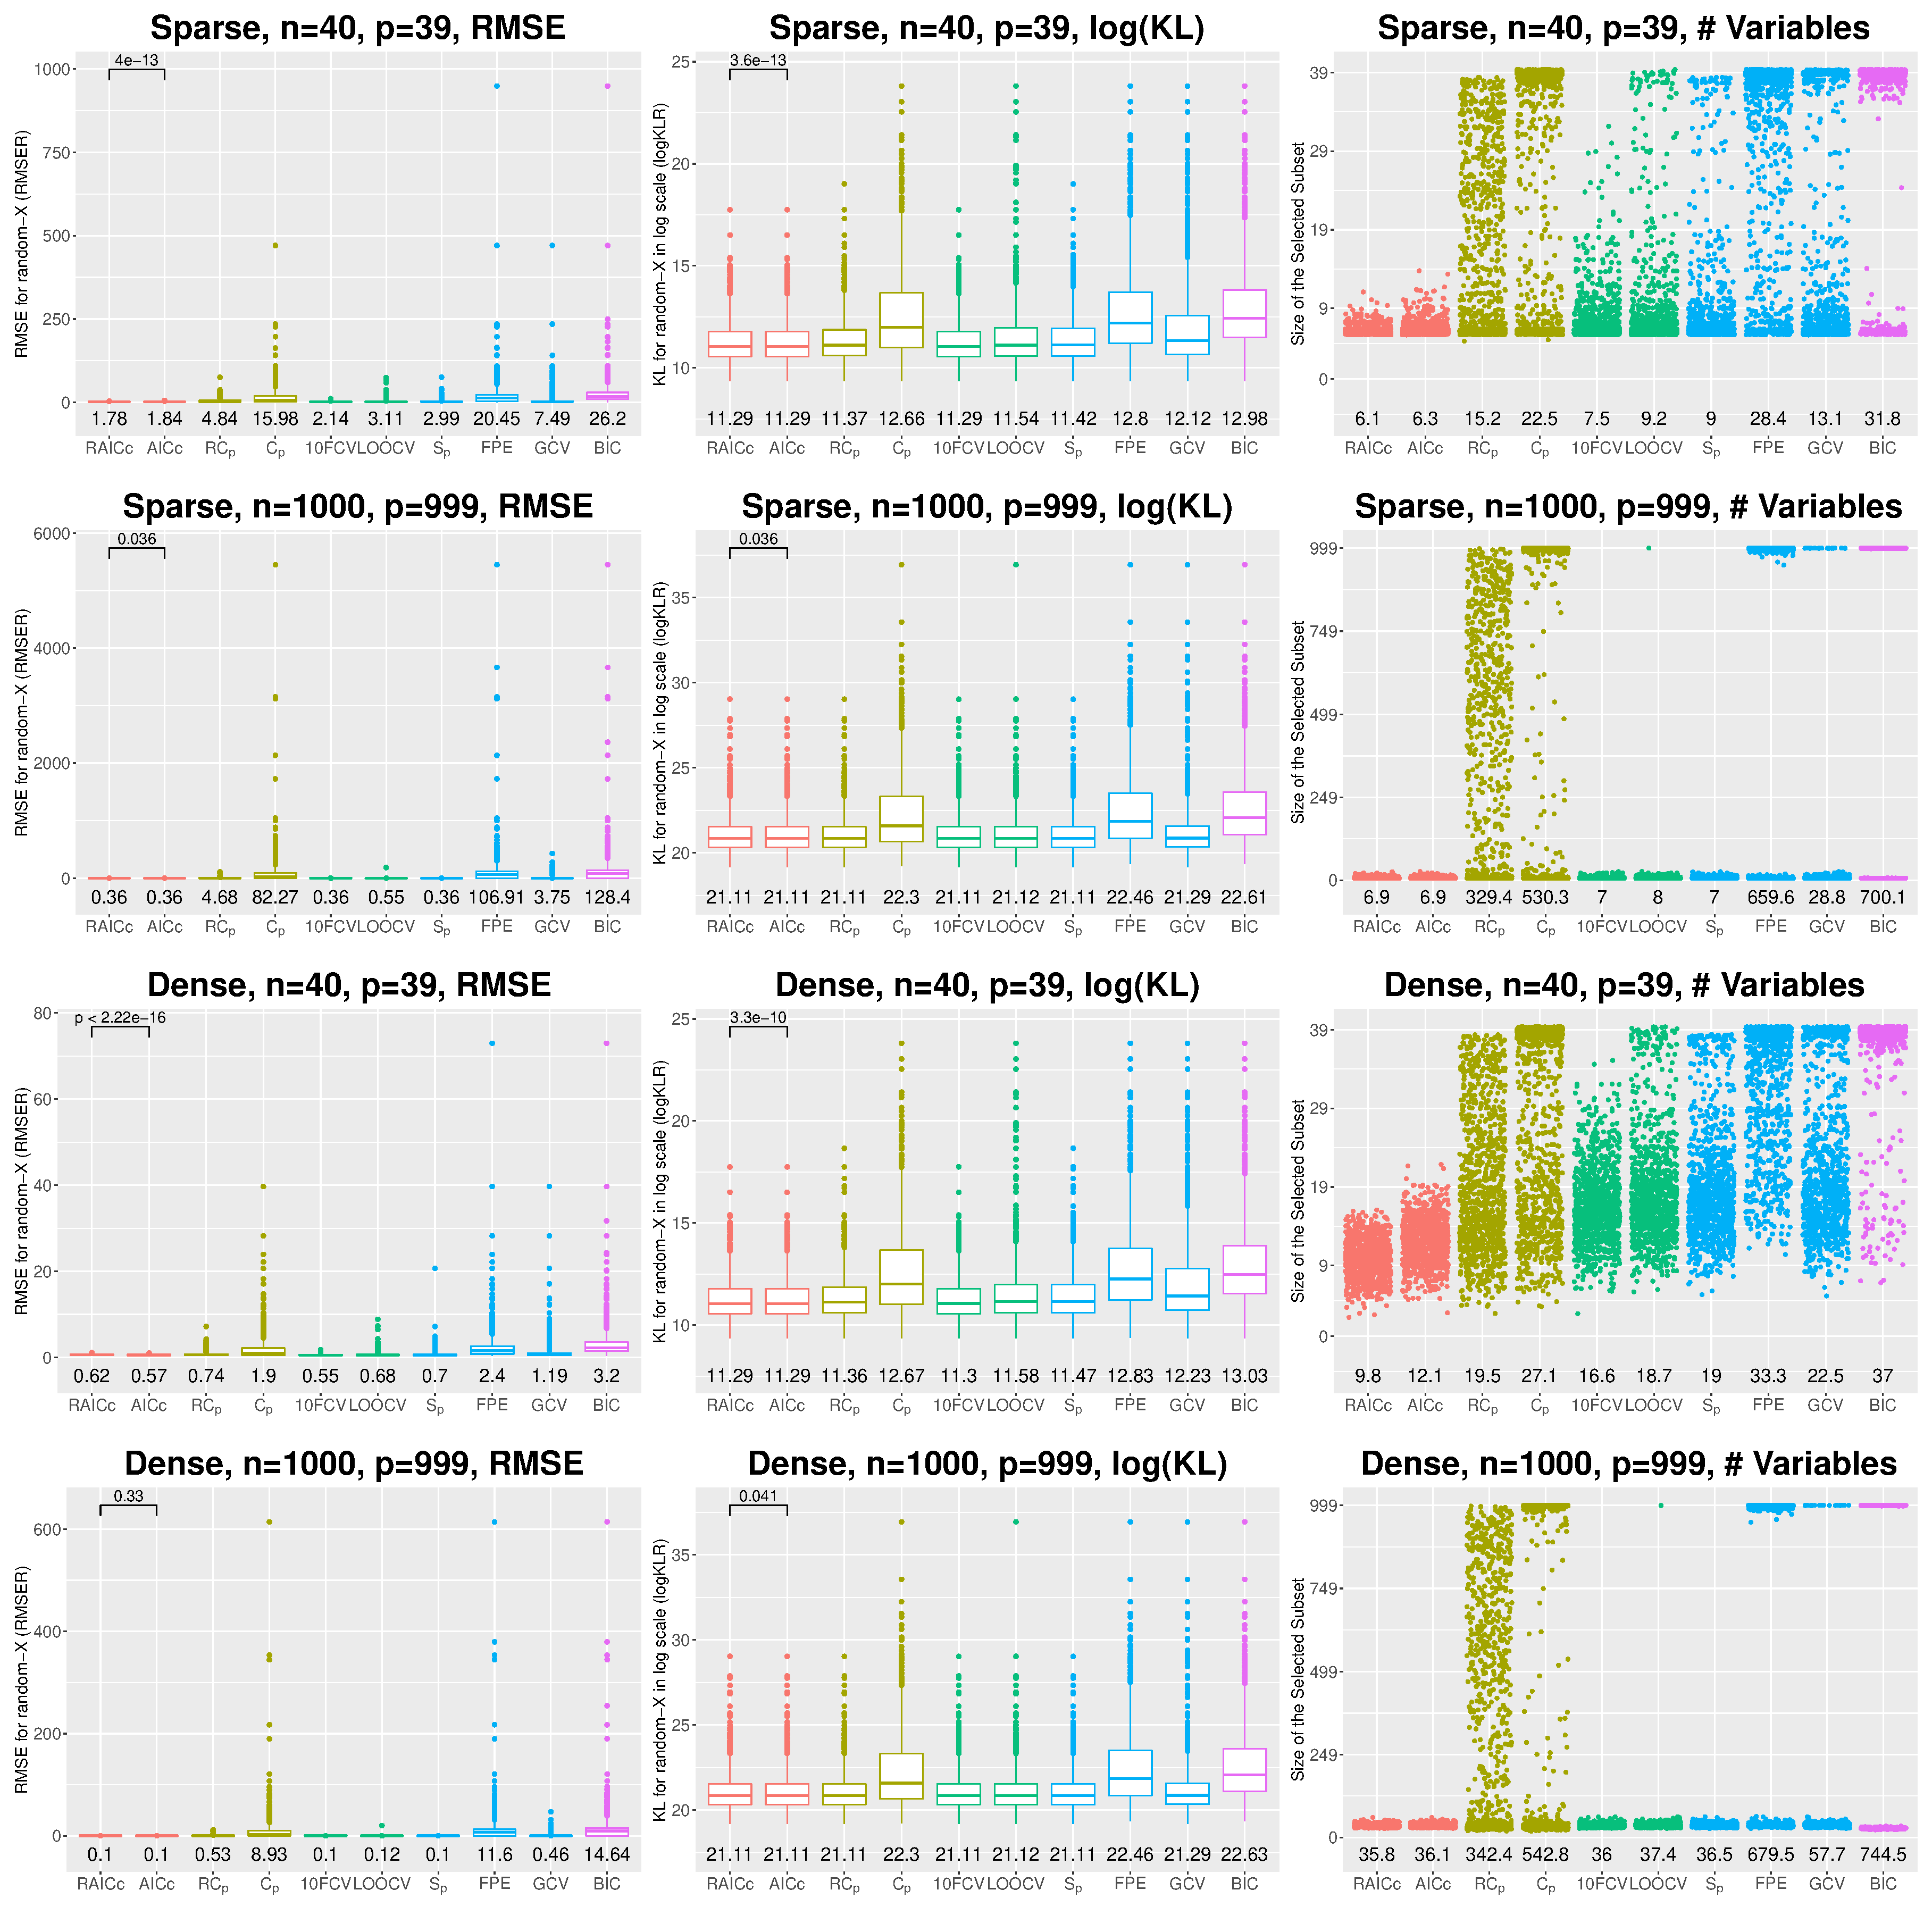
\includegraphics[width=\textwidth]{figures/main/randomx_VS_hsnr.eps}
  \caption{Results of simulations for variable selection. Random-X, high signal and $\rho=0.5$. The Sparse and Dense models correspond to the VS-Ex2 and VS-Ex3 configurations (details are given in the Online Supplemental Material). The first column refers to RMSE, the second column corresponds to KL discrepancy (in log scale), and the third column gives the number of variables in the selected model with nonzero slopes, jittered horizontally and vertically, so the number of models with that number of nonzero slopes can be ascertained more easily. The mean values of the evaluation metrics for each criterion are presented at the bottom of each graph. The p-values of the Wilcoxon signed-rank test (paired and two-sided) for comparing RAICc and AICc are also presented.}
  \label{fig:subsetselection_randomx_hsnr_largep}
\end{figure}


\begin{figure}[!ht]
  \centering
  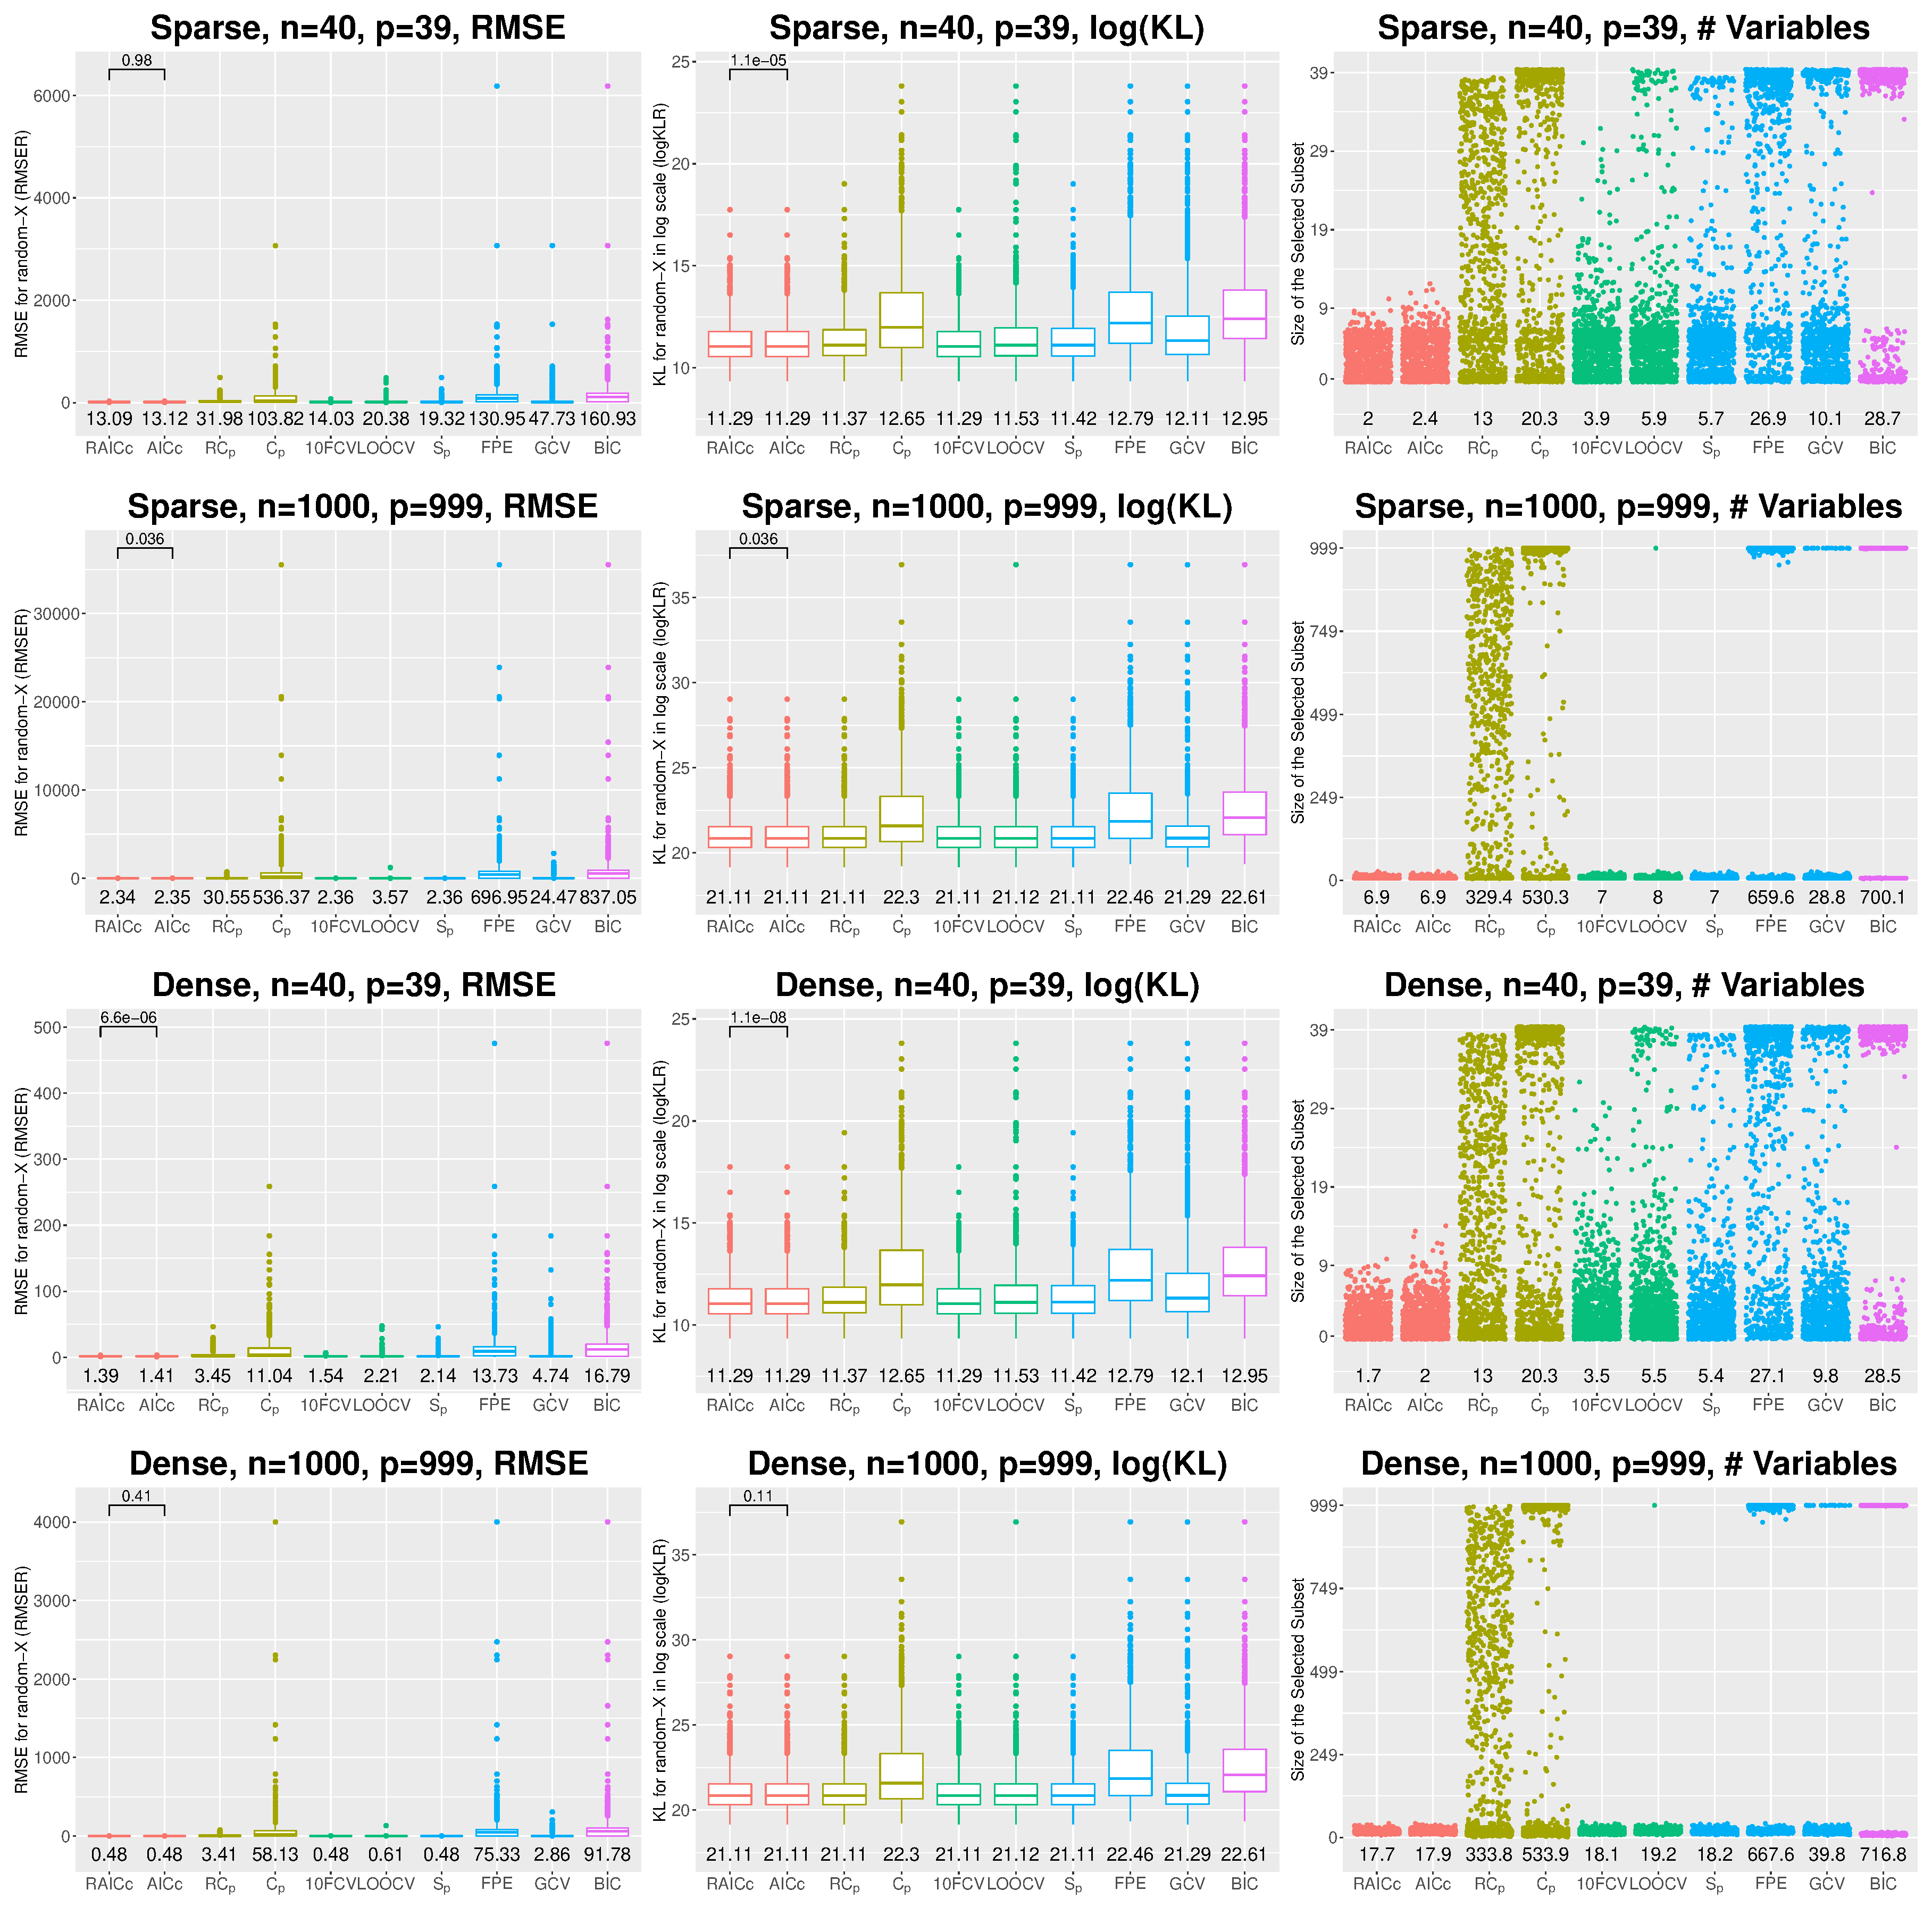
\includegraphics[width=\textwidth]{figures/main/randomx_VS_lsnr.eps}
  \caption{Results of simulations for variable selection. Random-X, low signal and $\rho=0.5$. }
  \label{fig:subsetselection_randomx_lsnr_largep}
\end{figure}

We next consider the general restriction problem. We take $\beta_0 = [2,2,2,1,1,1]^T$, $n\in\{10,40\}$, moderate correlations between the predictors, and either high or low signal levels. The candidate models are constructed in the following way. We consider a set of restrictions: $\beta_1=\beta_4$, $\beta_1=2\beta_2$, $\beta_1=\beta_2$, $\beta_2=\beta_3$, $\beta_4=\beta_5$, $\beta_5=\beta_6$, where the last four restrictions hold for our choice of $\beta_0$. We then consider all of the possible subsets of the six restrictions, resulting in $64$ candidate models in total. The detailed configurations and complete results for this and other examples of the general restriction problem ($54$ scenarios in total) are given in the Online Supplemental Material. 

We see from Figure \ref{fig:generalrestriction_randomx} that differences in performance between the criteria are less dramatic. This is not surprising, since for these models the number of parameters never approaches the sample size. Still, RAICc is consistently the best selection rule for small sample size $n$, and it is second-best for large $n$, where it is outperformed by BIC (note that BIC has a strong tendency to select too few restrictions when the sample is small, which corresponds to overfitting in the variable selection context). We also note an advantage of RAICc over AICc, with AICc having a stronger tendency to select too few restrictions.

\begin{figure}[!ht]
  \centering
  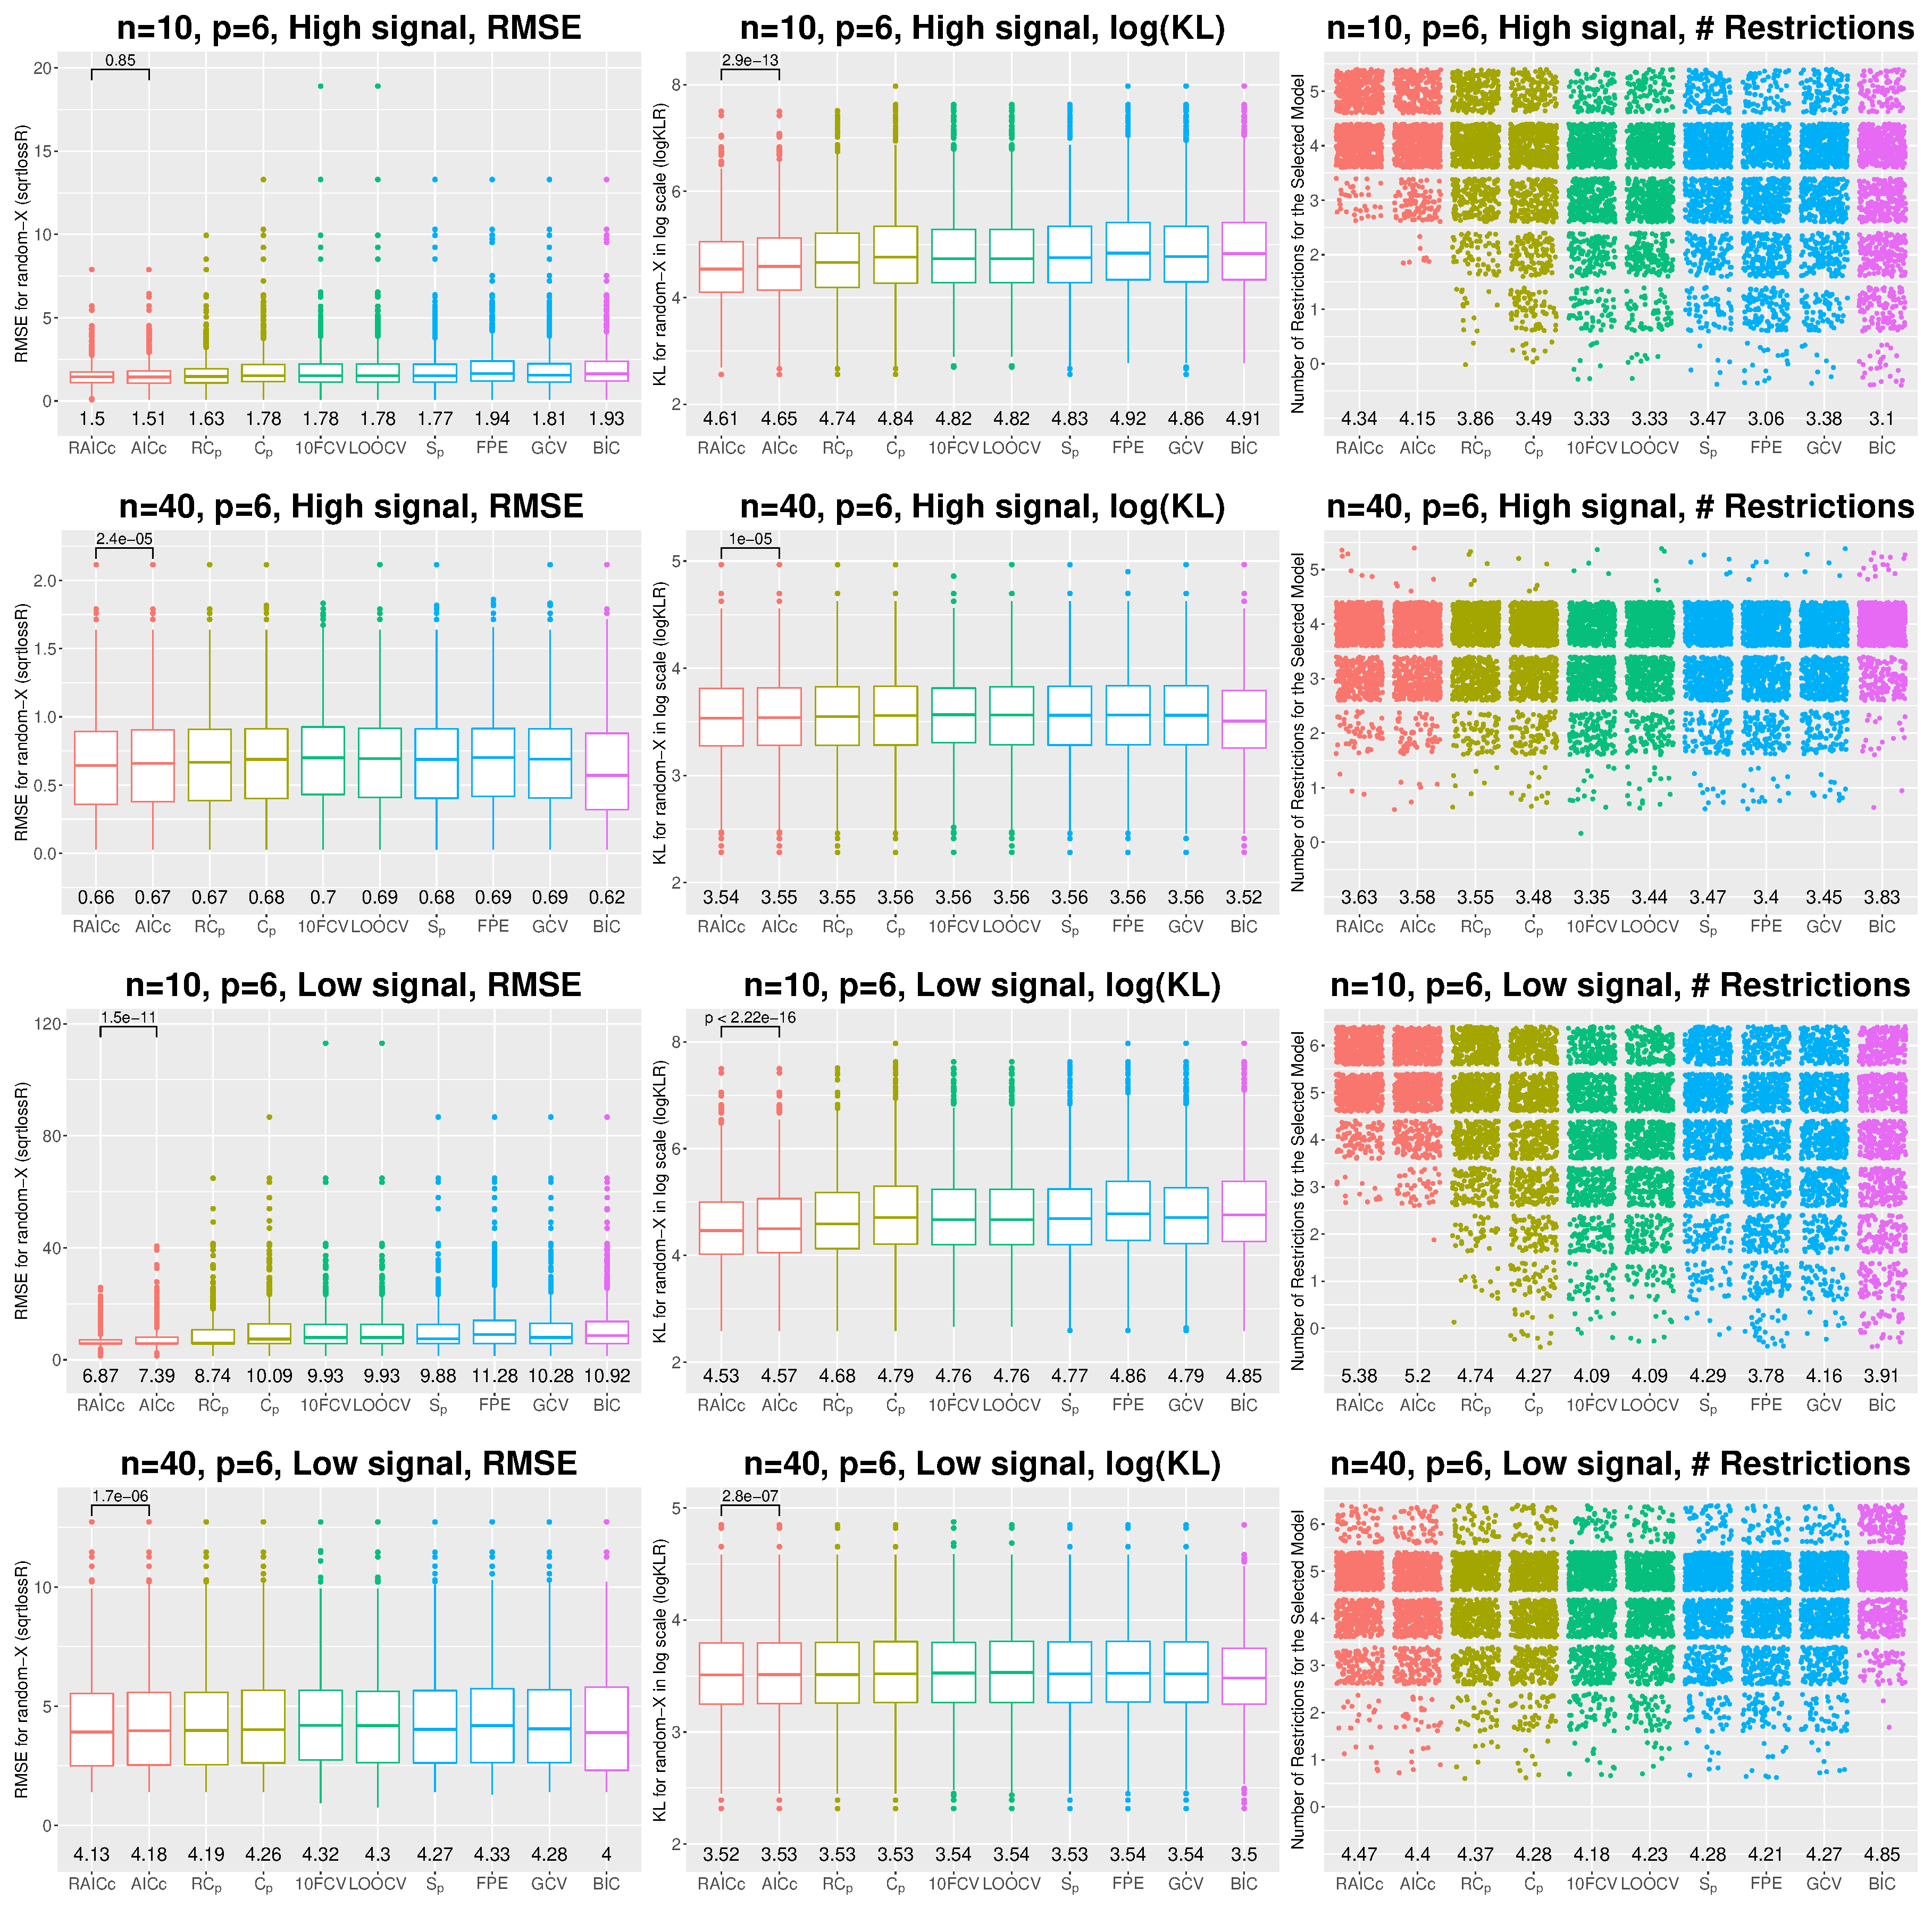
\includegraphics[width=\textwidth]{figures/main/randomx_GR-Ex1.eps}
  \caption{Results of simulations for general restrictions. Random-X, $\rho=0.5$. The configuration of the model is GR-Ex1 (details can be found in the Online Supplemental Material). Third column gives the number of variables in the number of restrictions in the selected models, jittered horizontally and vertically, so the number of models with that number of imposed restrictions can be ascertained more easily. The mean values of the evaluation metrics for each criterion are presented at the bottom of each graph. The p-values of the Wilcoxon signed-rank test (paired and two-sided) for comparing RAICc and AICc are also presented.}
  \label{fig:generalrestriction_randomx}
\end{figure}

Finally, we extend the general restriction example by including restrictions that force additional predictors to have zero coefficients (as in the variable selection problem). Besides the six restrictions specified, we also consider $\beta_i=0$ for $i=7,\cdots,p$ resulting in $p$ possible restrictions in total. The candidate models are formulated by excluding the restrictions in a nested fashion. We start from the model including all $p$ restrictions (corresponding to the null model), and the next model includes the $p-1$ restrictions except the first one $\beta_1=\beta_4$. The process is repeated until all restrictions are excluded (the full model including all predictors with arbitrary slopes) resulting in $p+1$ candidate models in total. The true coefficient vector is the same as that used in Figure \ref{fig:generalrestriction_randomx}, implying that the correct number of restrictions is $p-2$. We present the detailed configurations and complete results for this and other examples ($243$ scenarios in total) in the Online Supplemental Material. 

We see from Figure \ref{fig:subsetgeneral_randomx} that our findings for the variable selection problem also hold in this case. This is not surprising, since variable selection is just a special example of general restrictions, and in this scenario the set of candidate models includes ones where the number of parameters is close to the sample size. Thus, overall, RAICc and AICc are the best performers among all of the selectors. RAICc tends to provide the sparsest subset (or select more restrictions), while rarely underfitting, having a slight advantage over AICc in terms of predictive performance. 

\begin{figure}[!ht]
  \centering
  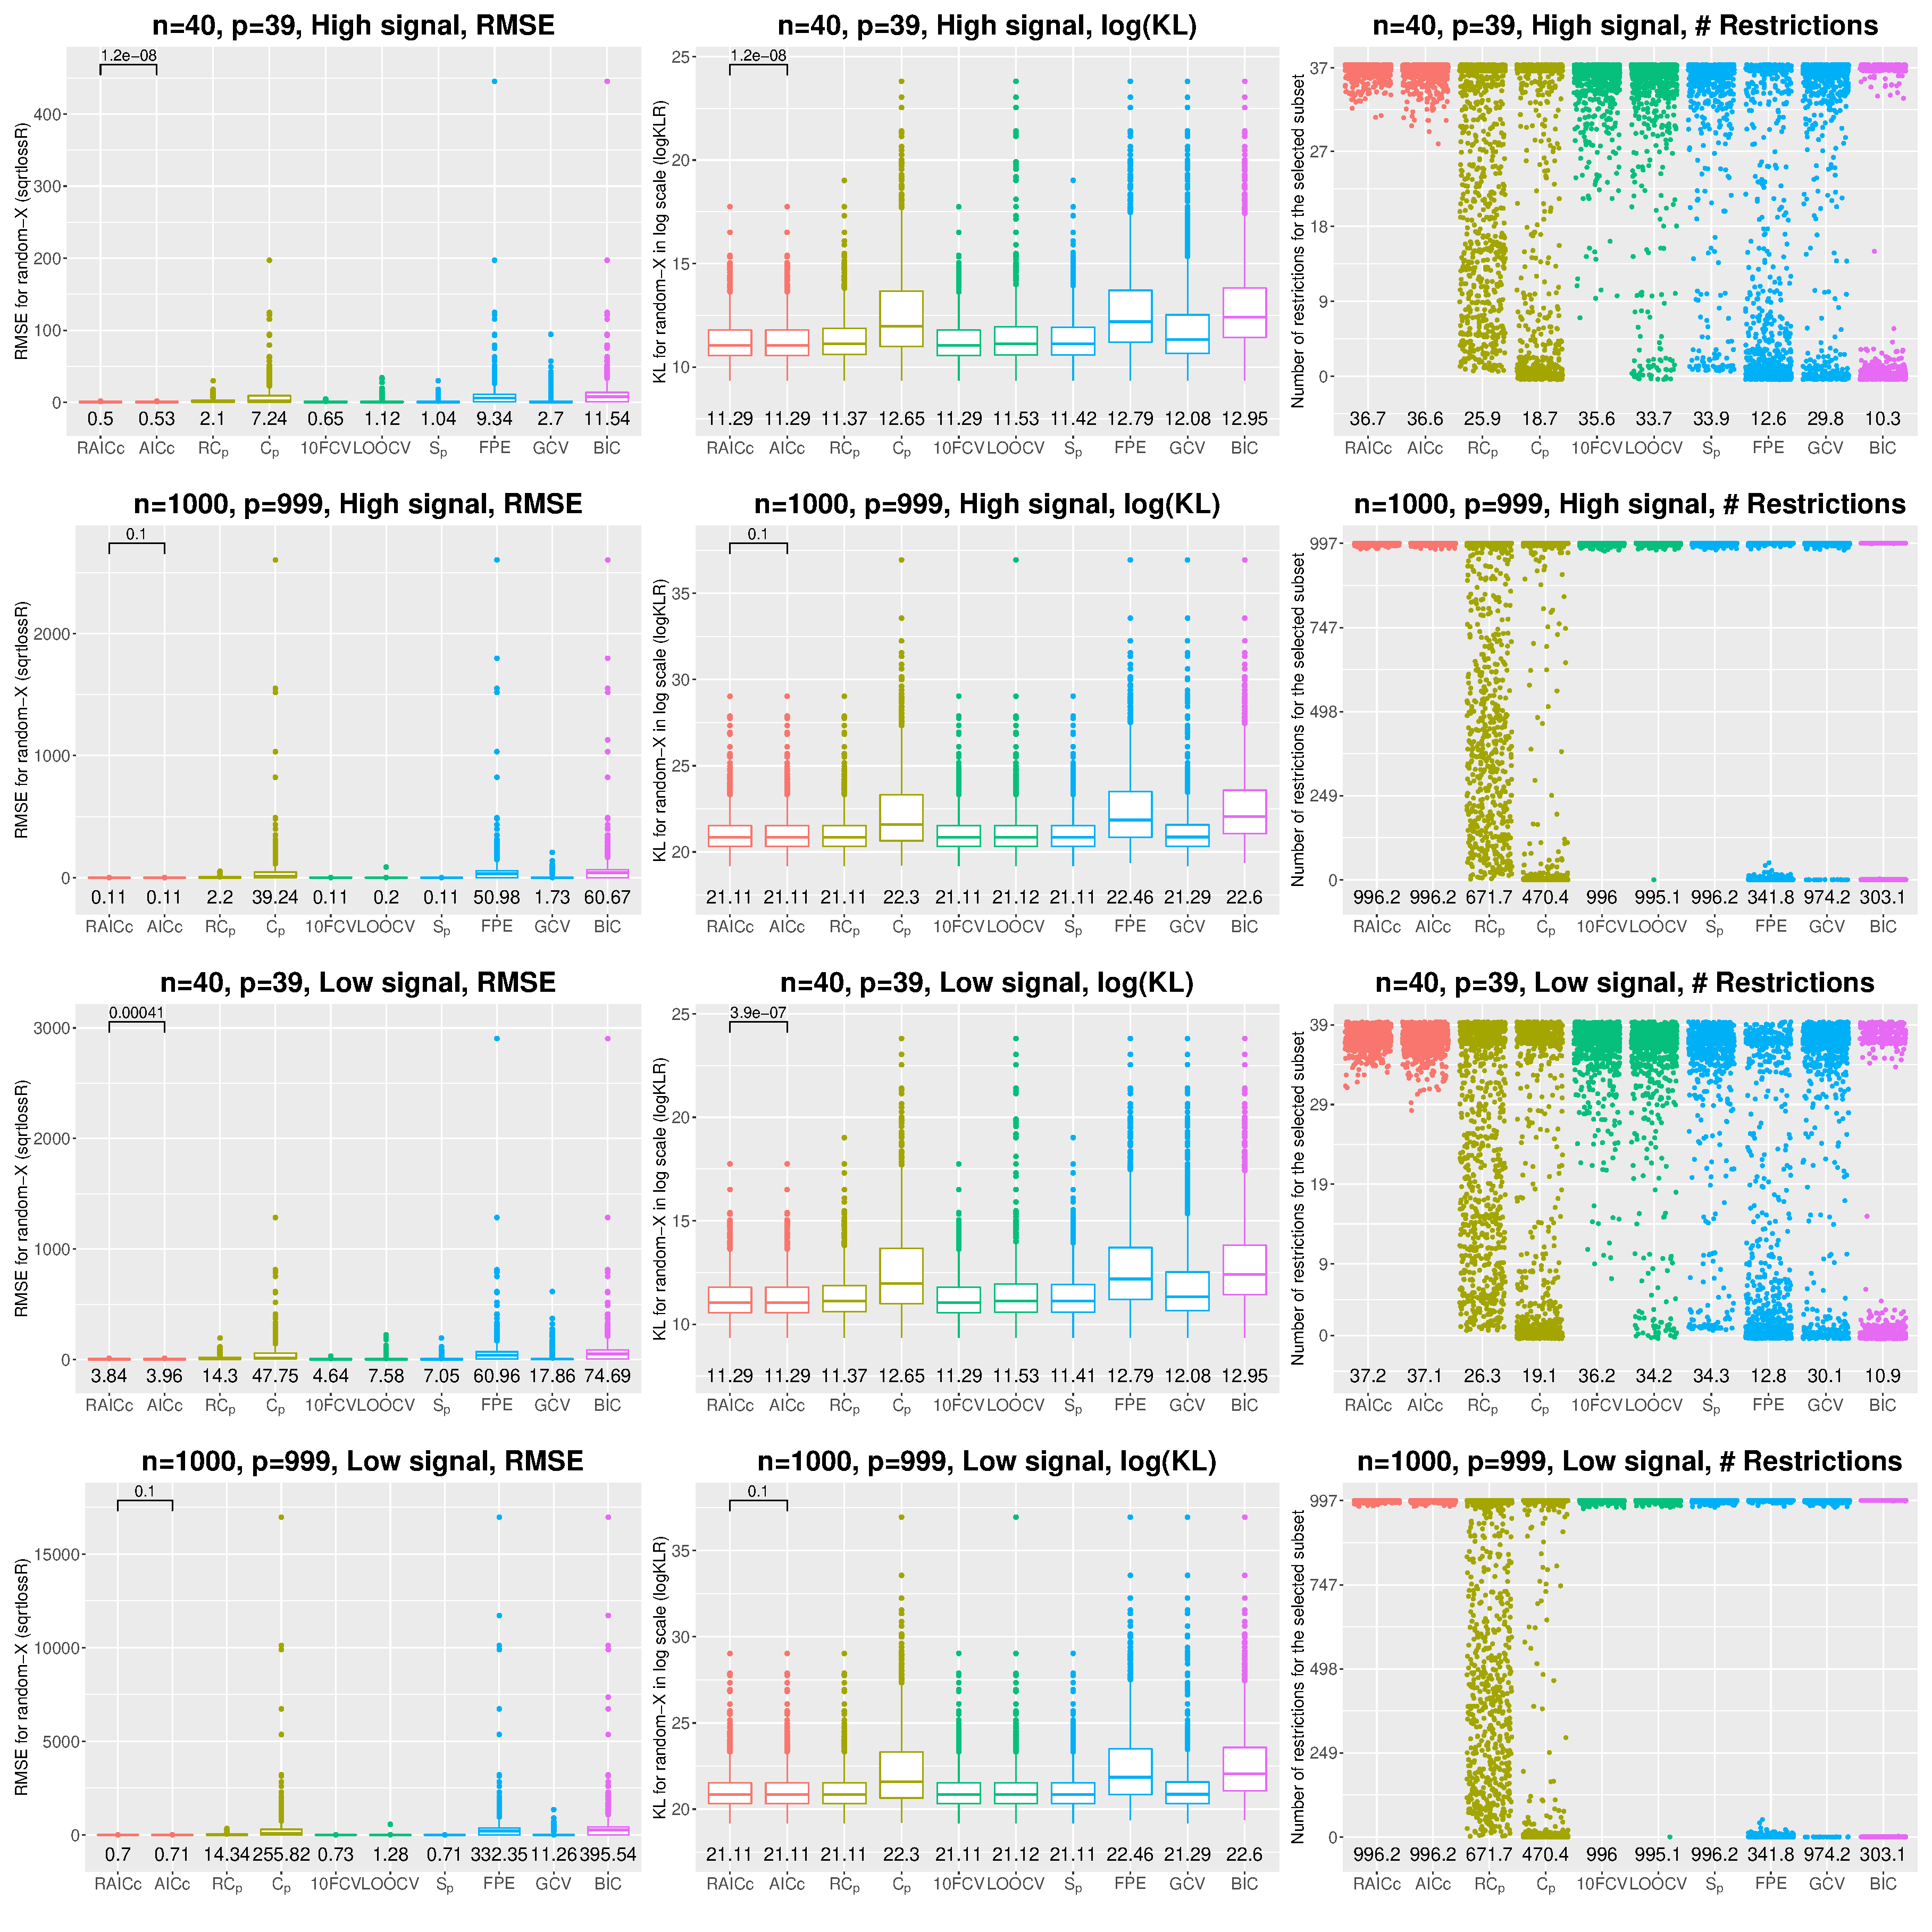
\includegraphics[width=\textwidth]{figures/main/randomx_GR-Ex4.eps}
  \caption{Results of simulations for general restrictions. Random-X, $\rho=0.5$. The configuration of the model is GR-Ex4 (details can be found in the Online Supplemental Material).}
  \label{fig:subsetgeneral_randomx}
\end{figure}

\iffalse
\subsubsection{Without a true model}
\begin{itemize}
	\item Omit: The configuration is the same as Sparse-Ex1, but with the 6-th predictor treated as missing for all the fitting procedures.
	\item Exponential: We take $\Sigma = I$. The responses are generated by $y_i=exp(4i/n) + \epsilon_i$, for $i=1,\cdots,n$, where $\epsilon_i$ are independent $\mathcal{N}(0, \sigma_0^2)$. 
\end{itemize}
	We consider a fixed trigonometric configuration of $X$ that is studied by \citet{Hurvich1991}, where $X$ is an $n$ by $p$ matrix with components defined by 
$$ x_{t, 2j-1} = \sin\left(\frac{2\pi j}{n}t\right),$$
and 
$$ x_{t,2j} = \cos\left(\frac{2\pi j}{n}t\right),$$
for $j=1,\cdots,p/2$ and $t=0,\cdots,n-1$. The responses are generated by $y_i=exp(4i/n) + \epsilon_i$, for $i=1,\cdots,n$, where $\epsilon_i$ are independent $\mathcal{N}(0, \sigma_0^2)$. 
\fi



\iffalse
\begin{figure}[!ht]
  \centering
  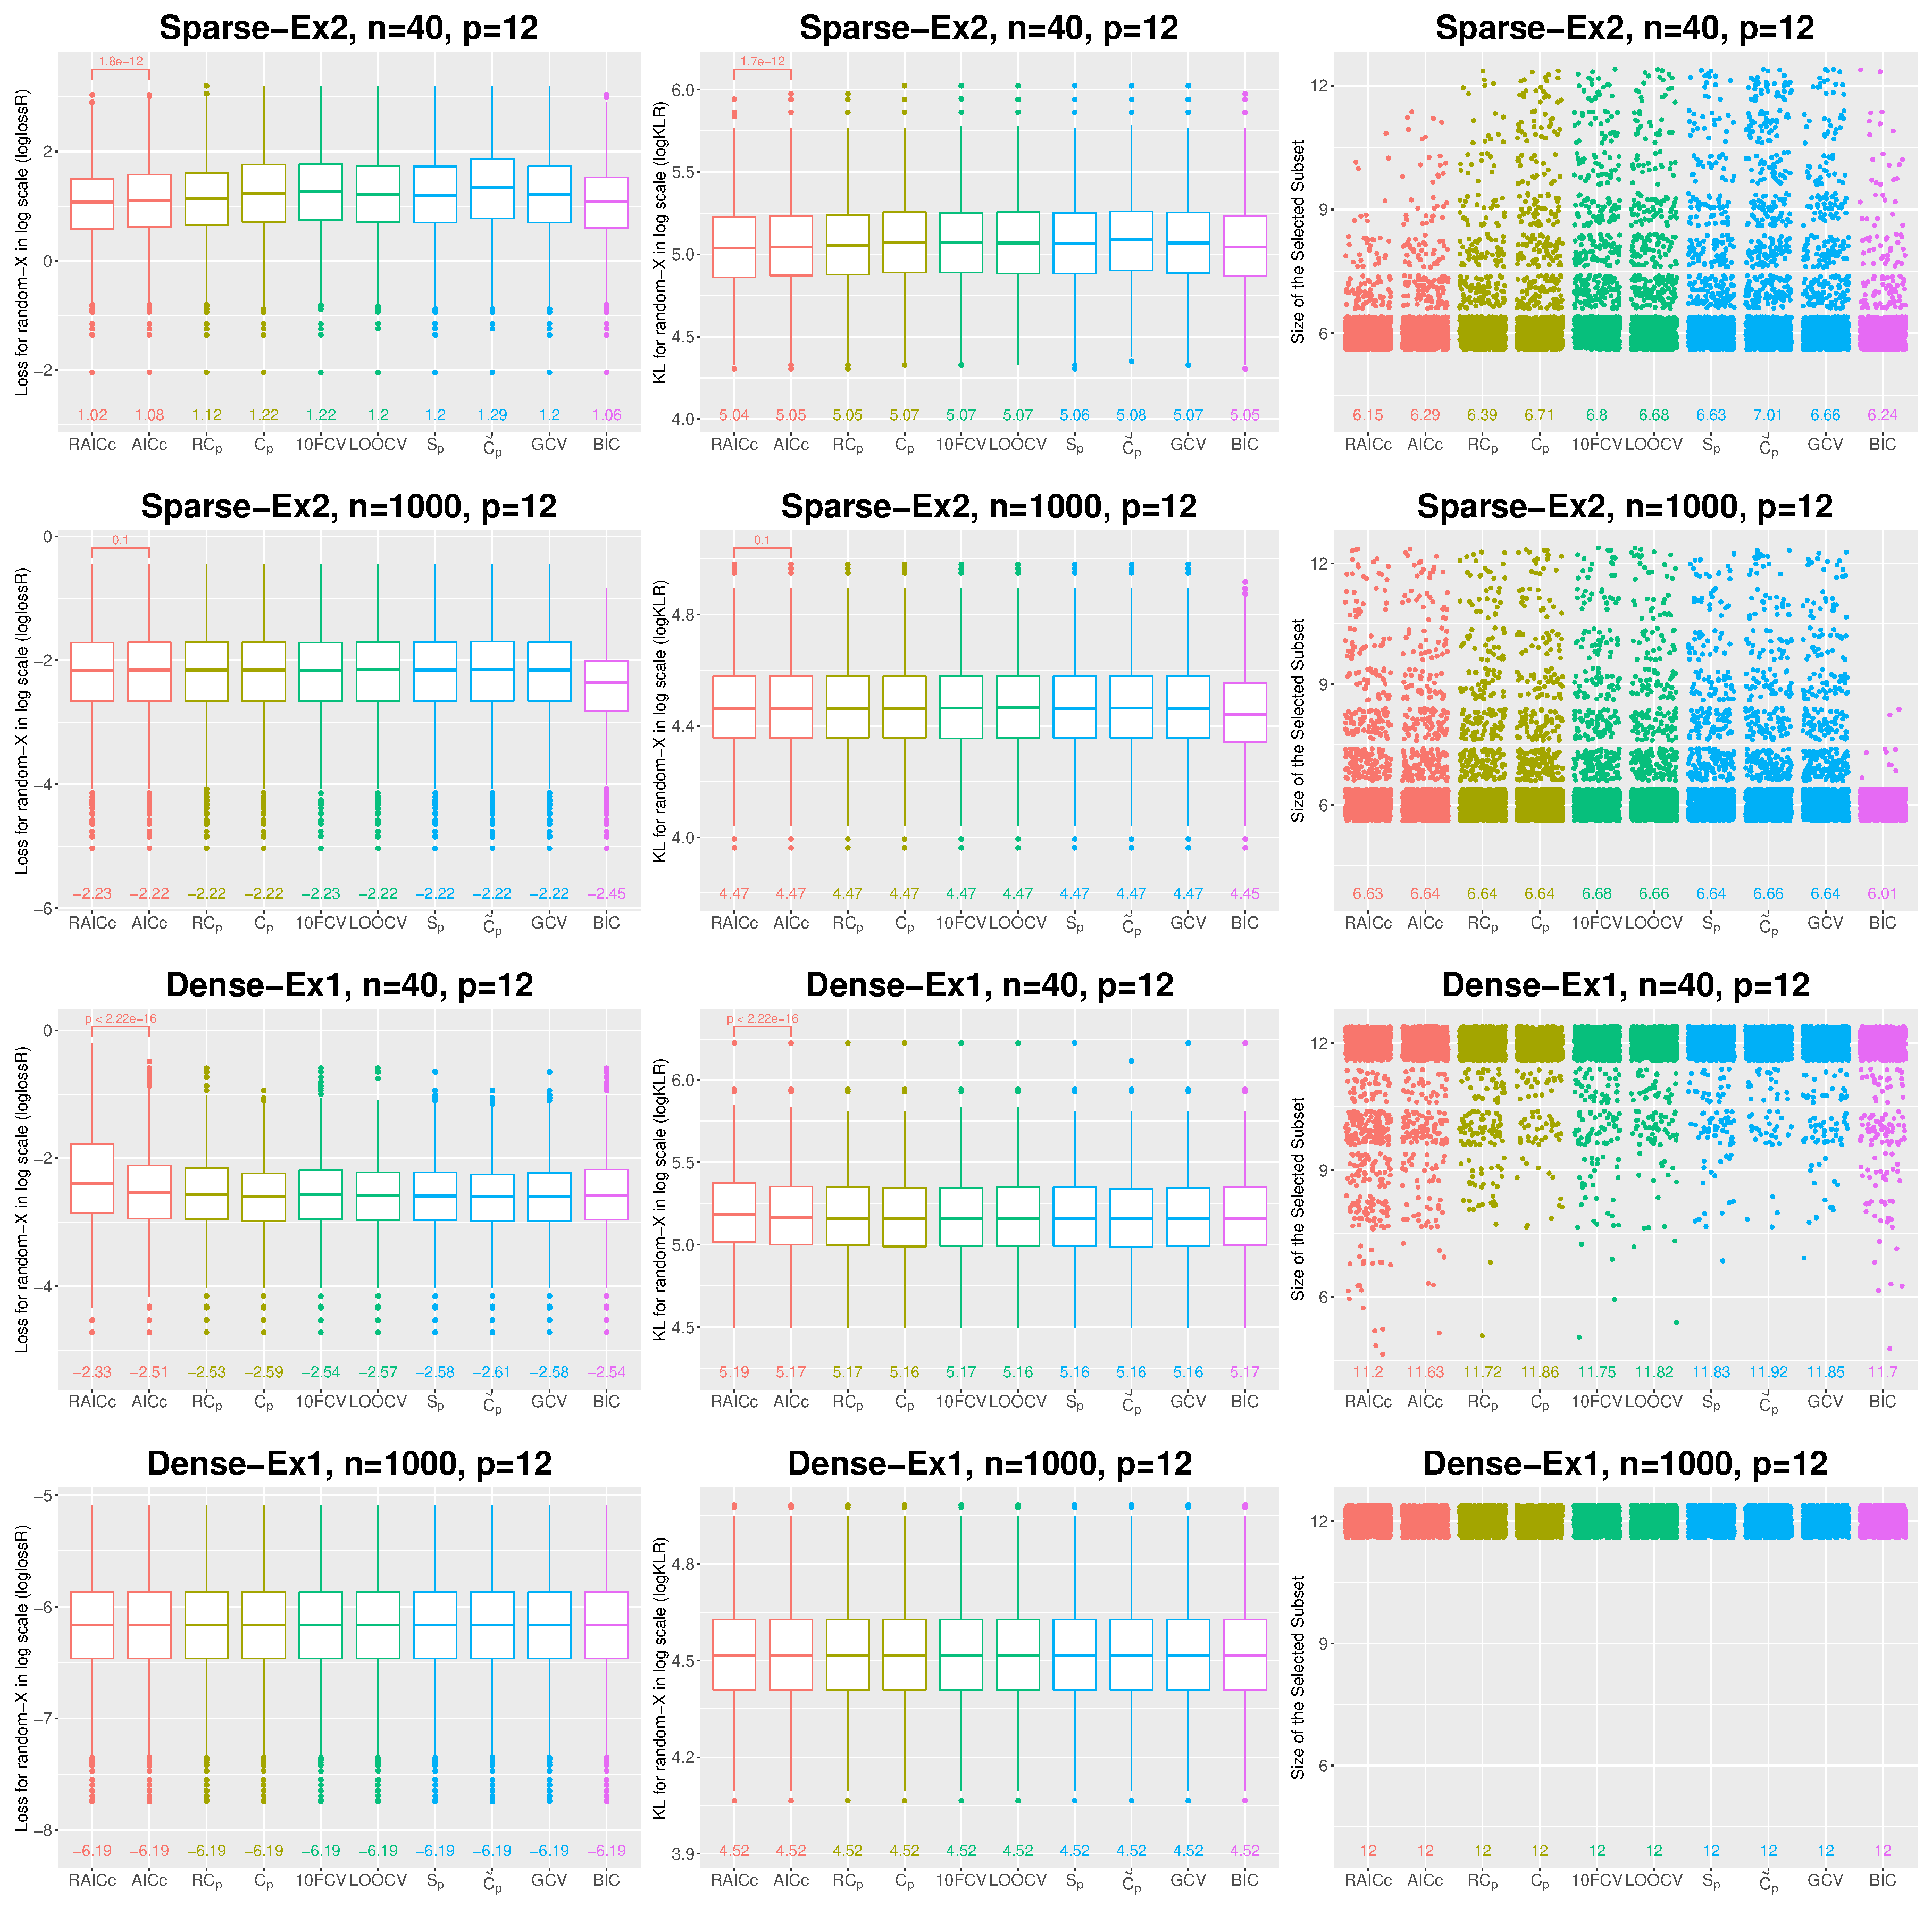
\includegraphics[width=\textwidth]{figures/main/randomx/subset_selection/smallp_hsnr.eps}
  \caption{Random-X, high signal and $\rho=0.5$. The mean values of the evaluation metrics for each criterion are presented at the bottom of each graph. The p-values of the Wilcoxon signed-rank test (paired and two-sided) for comparing RAICc and AICc are also presented.}
  \label{fig:subsetselection_randomx_hsnr_smallp}
\end{figure}

\begin{figure}[!ht]
  \centering
  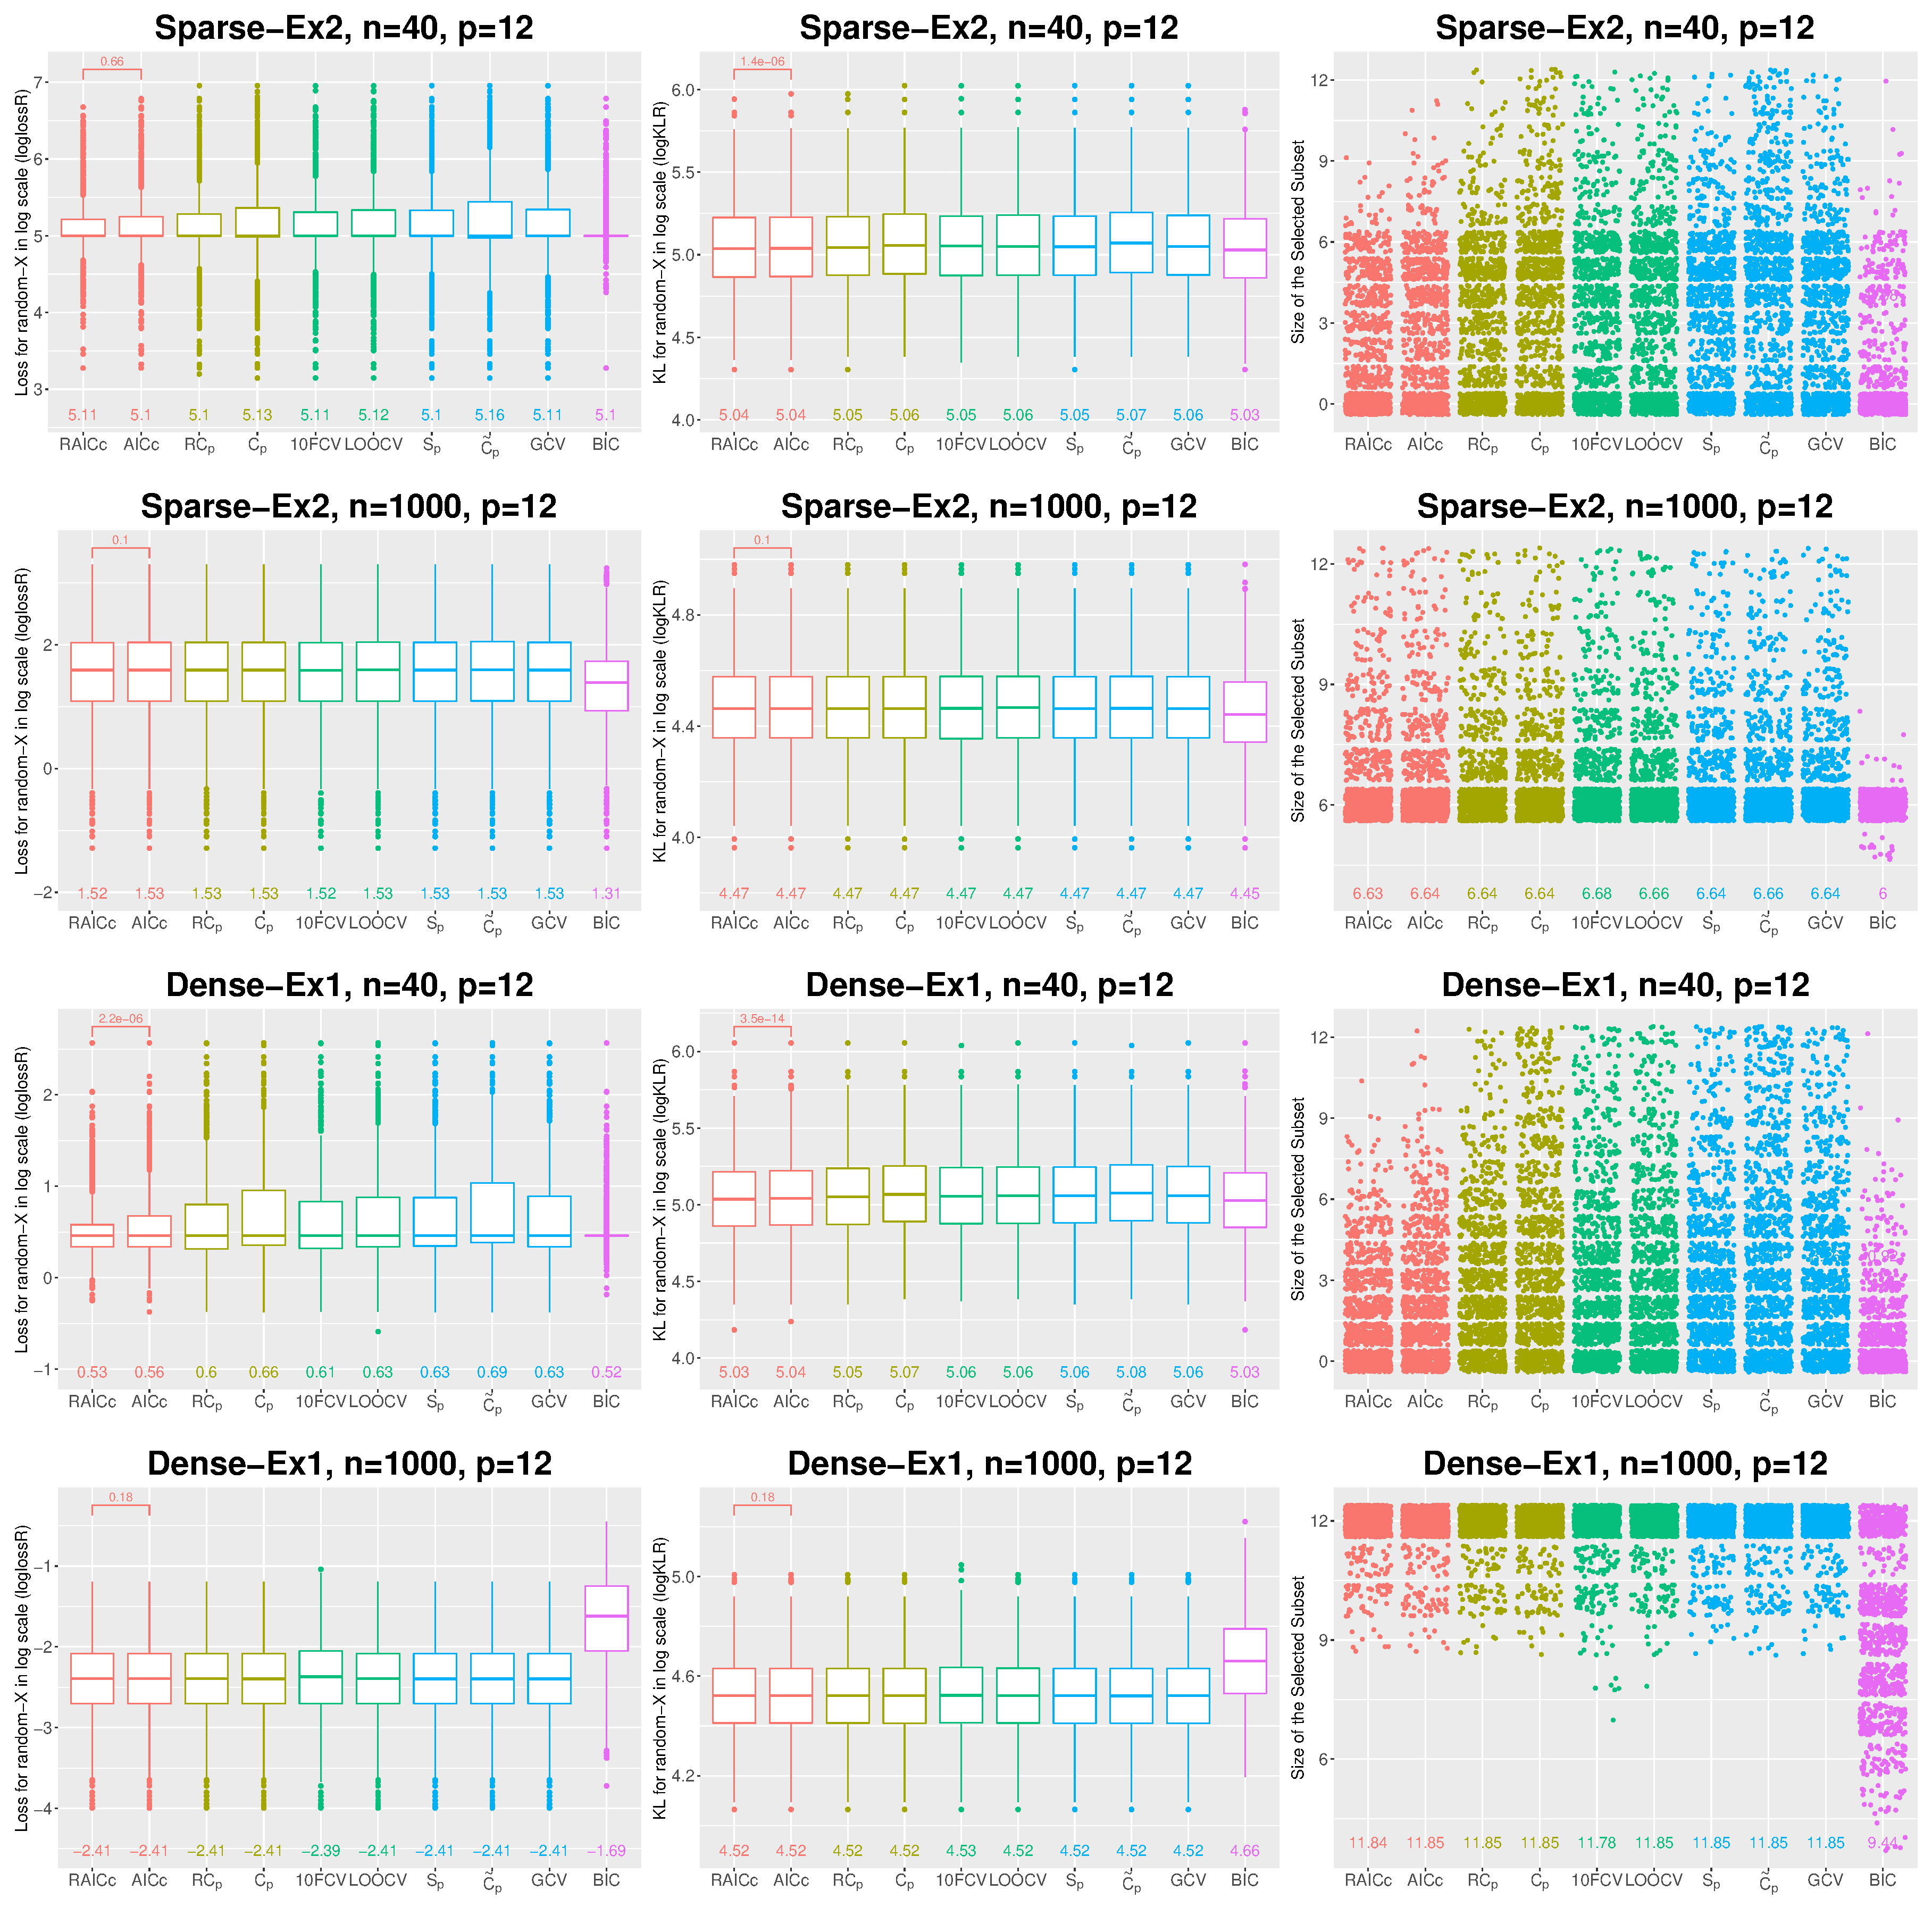
\includegraphics[width=\textwidth]{figures/main/randomx/subset_selection/smallp_lsnr.eps}
  \caption{Random-X, low signal and $\rho=0.5$. Other details are the same as in Figure \ref{fig:randomx_hsnr_smallp}.}
  \label{fig:subsetselection_randomx_lsnr_smallp}
\end{figure}
\fi




\subsection{Fixed-X}
The simulation structure for random-X can also be applied to fixed-X. We only generate the design matrix $X$ once and draw $1000$ replications of the response vector $y$ from the conditional distribution of $y|X$ based on \eqref{eq:truemodel}. The evaluation metrics for fixed-X are as follows. The complete simulation results are given in the Online Supplemental Material. 
\begin{itemize}
  \item Root mean squared error for fixed-X:
  \begin{equation*}
    \text{RMSEF} = \sqrt{ \frac{1}{n}\lVert X\hat\beta-X\beta_0 \rVert_2^2 }.
  \end{equation*} 

  \item KL discrepancy for fixed-X \eqref{eq:KLF} in the log scale (denoted as logKLF).

  \item Size of the subset selected.
\end{itemize}

The patterns for the fixed-X scenario are similar to those for random-X, as can be seen in Figures \ref{fig:subsetselection_fixedx_hsnr_largep}, \ref{fig:subsetselection_fixedx_lsnr_largep}, \ref{fig:generalrestriction_fixedx} and \ref{fig:subsetgeneral_fixedx}. In some ways this is surprising, in that the random-X versions of the criteria still seem to outperform the fixed-X versions, even though that is not the scenario for which they are designed. This seems to be related to the tendency for the fixed-X versions to overfit (or choose too few restrictions) compared to their random-X counterparts, which apparently works against the goal of selecting the candidate with best predictive performance. Otherwise, the KL-based criteria (RAICc and AICc) noticeably outperform the other criteria in general, especially $\mbox{C}_p$ and FPE, particularly for small samples.

\begin{figure}[!ht]
  \centering
  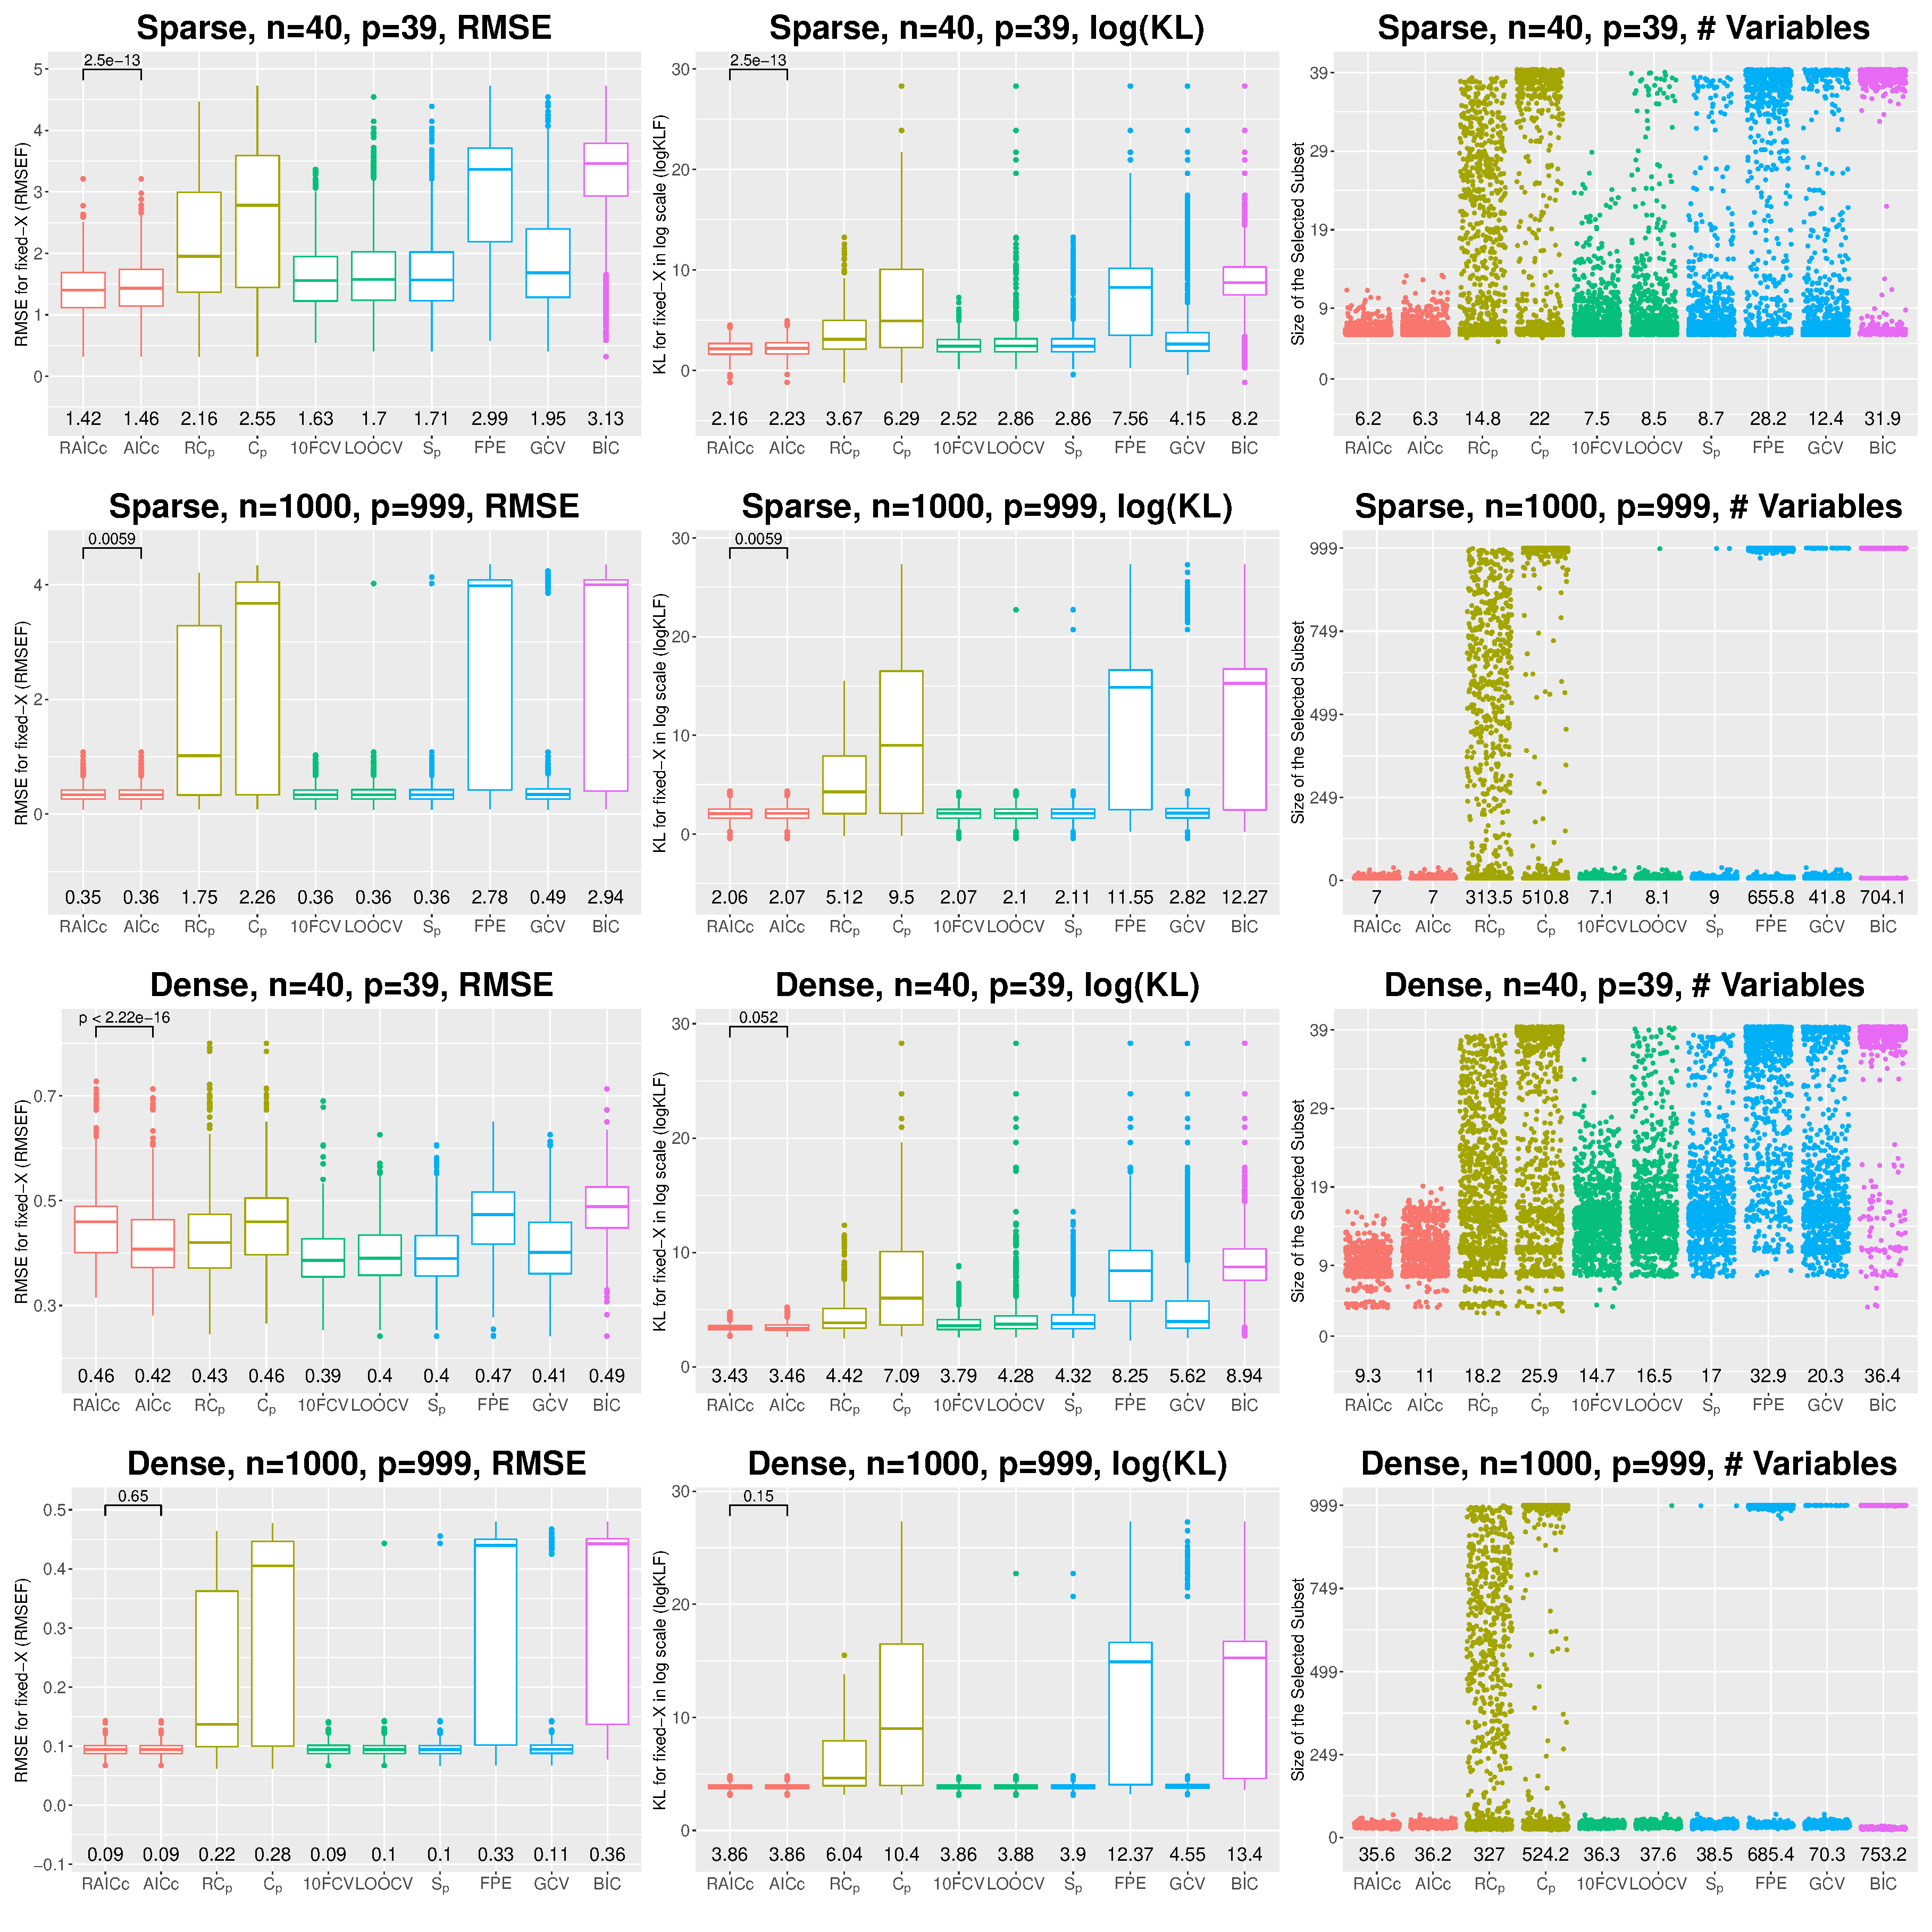
\includegraphics[width=\textwidth]{figures/main/fixedx_VS_hsnr.eps}
  \caption{Results of simulations for variable selection. Fixed-X, high signal. The configurations are the same as in Figure \ref{fig:subsetselection_randomx_hsnr_largep}.}
  \label{fig:subsetselection_fixedx_hsnr_largep}
\end{figure}


\begin{figure}[!ht]
  \centering
  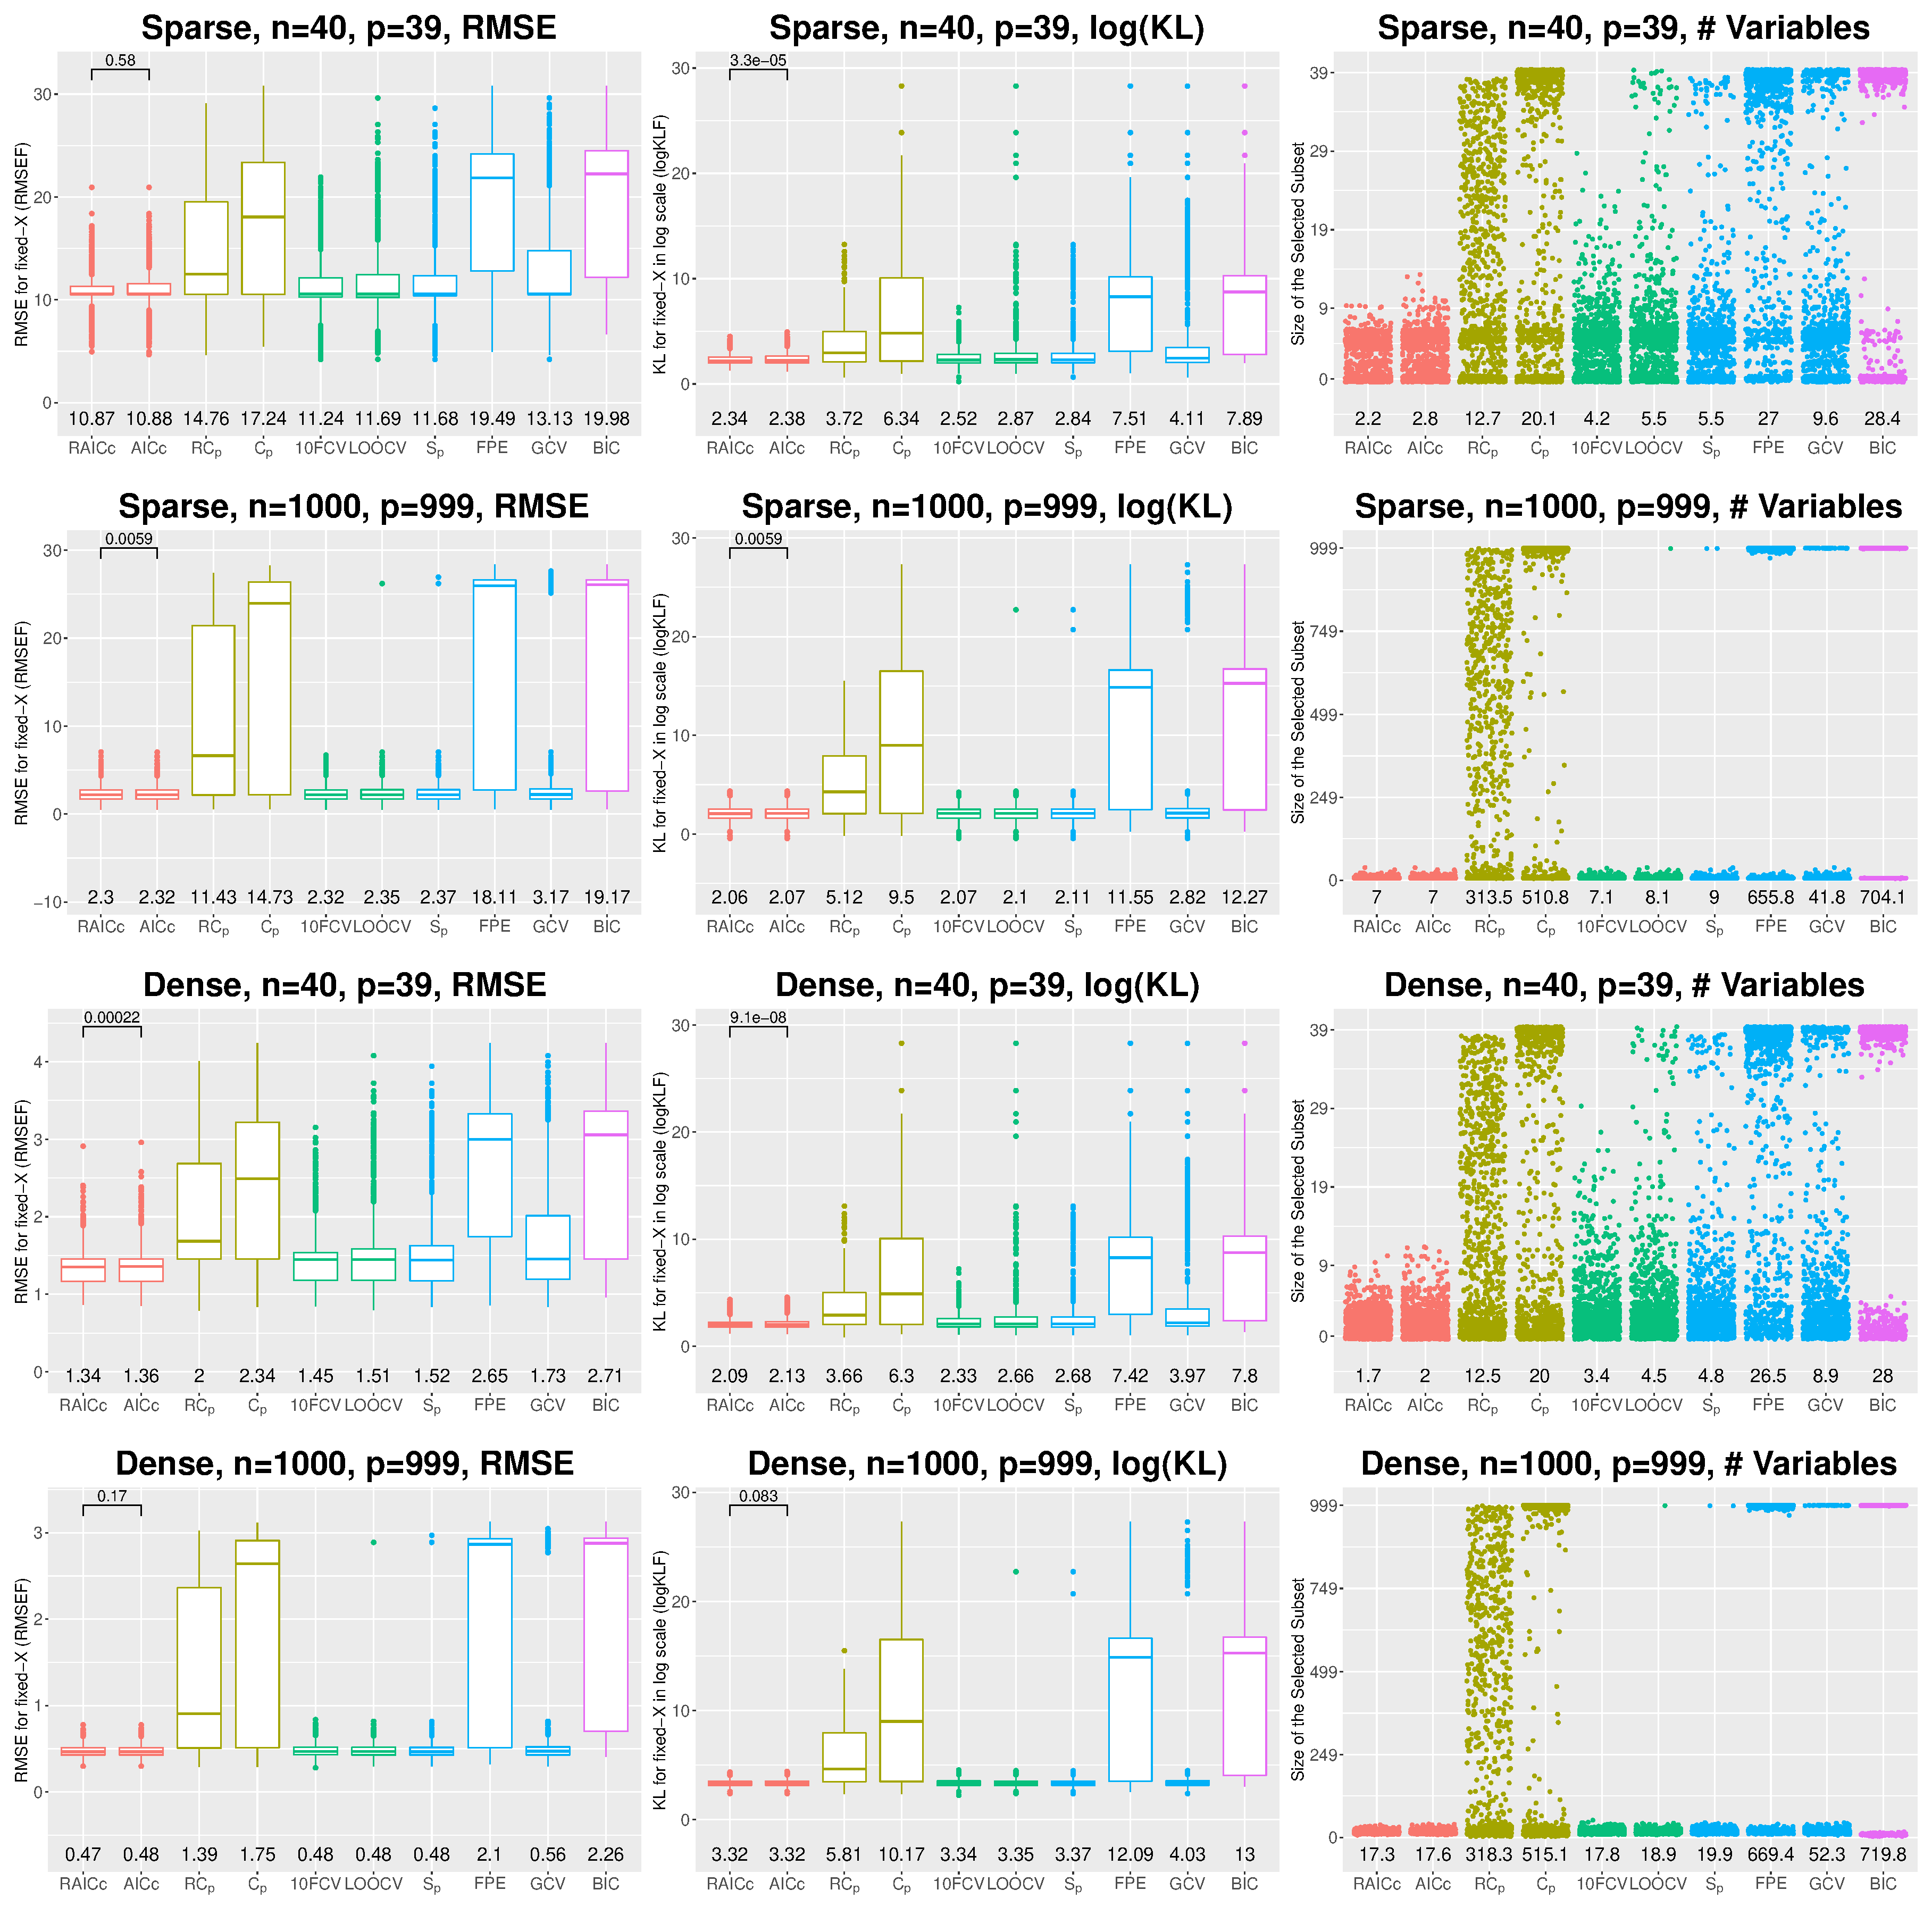
\includegraphics[width=\textwidth]{figures/main/fixedx_VS_lsnr.eps}
  \caption{Results of simulations for variable selection. Fixed-X, low signal. The configurations are the same as in Figure \ref{fig:subsetselection_randomx_lsnr_largep}.}
  \label{fig:subsetselection_fixedx_lsnr_largep}
\end{figure}

\begin{figure}[!ht]
  \centering
  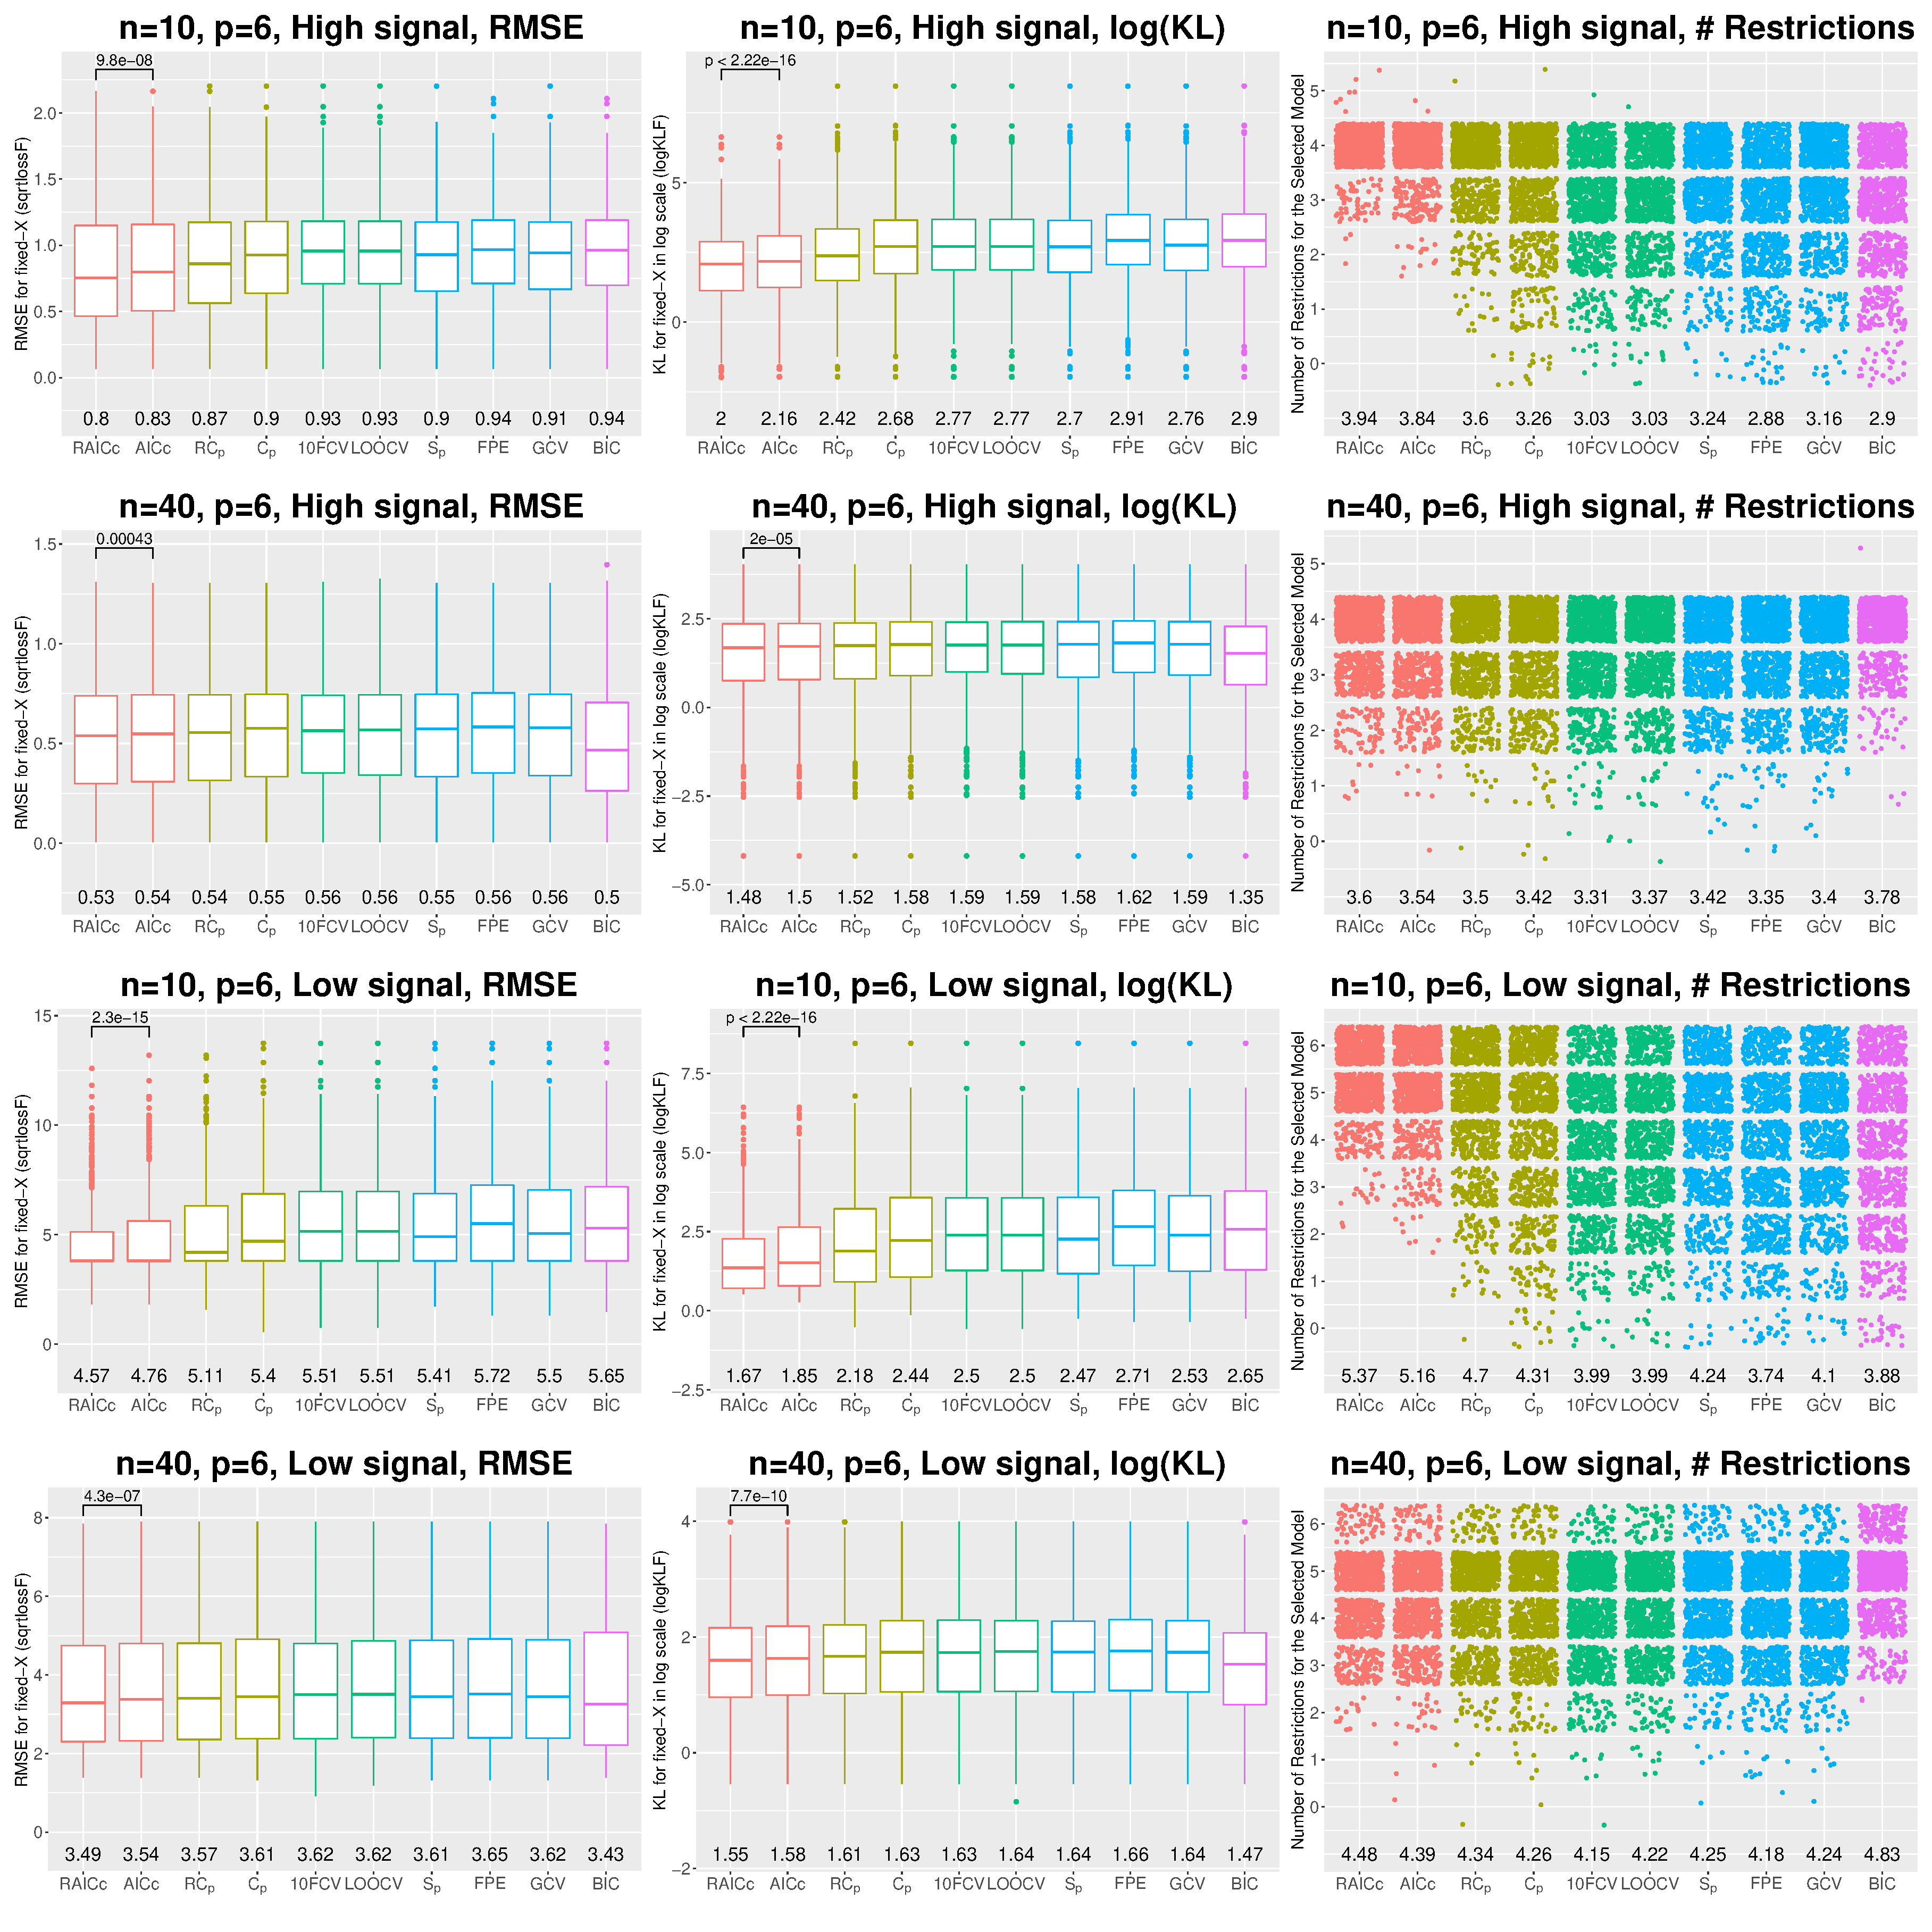
\includegraphics[width=\textwidth]{figures/main/fixedx_GR-Ex1.eps}
  \caption{Results of simulations for general restrictions. Fixed-X, GR-Ex1, $\rho=0.5$. The configurations are the same as in Figure \ref{fig:generalrestriction_randomx}.}
  \label{fig:generalrestriction_fixedx}
\end{figure}

\begin{figure}[!ht]
  \centering
  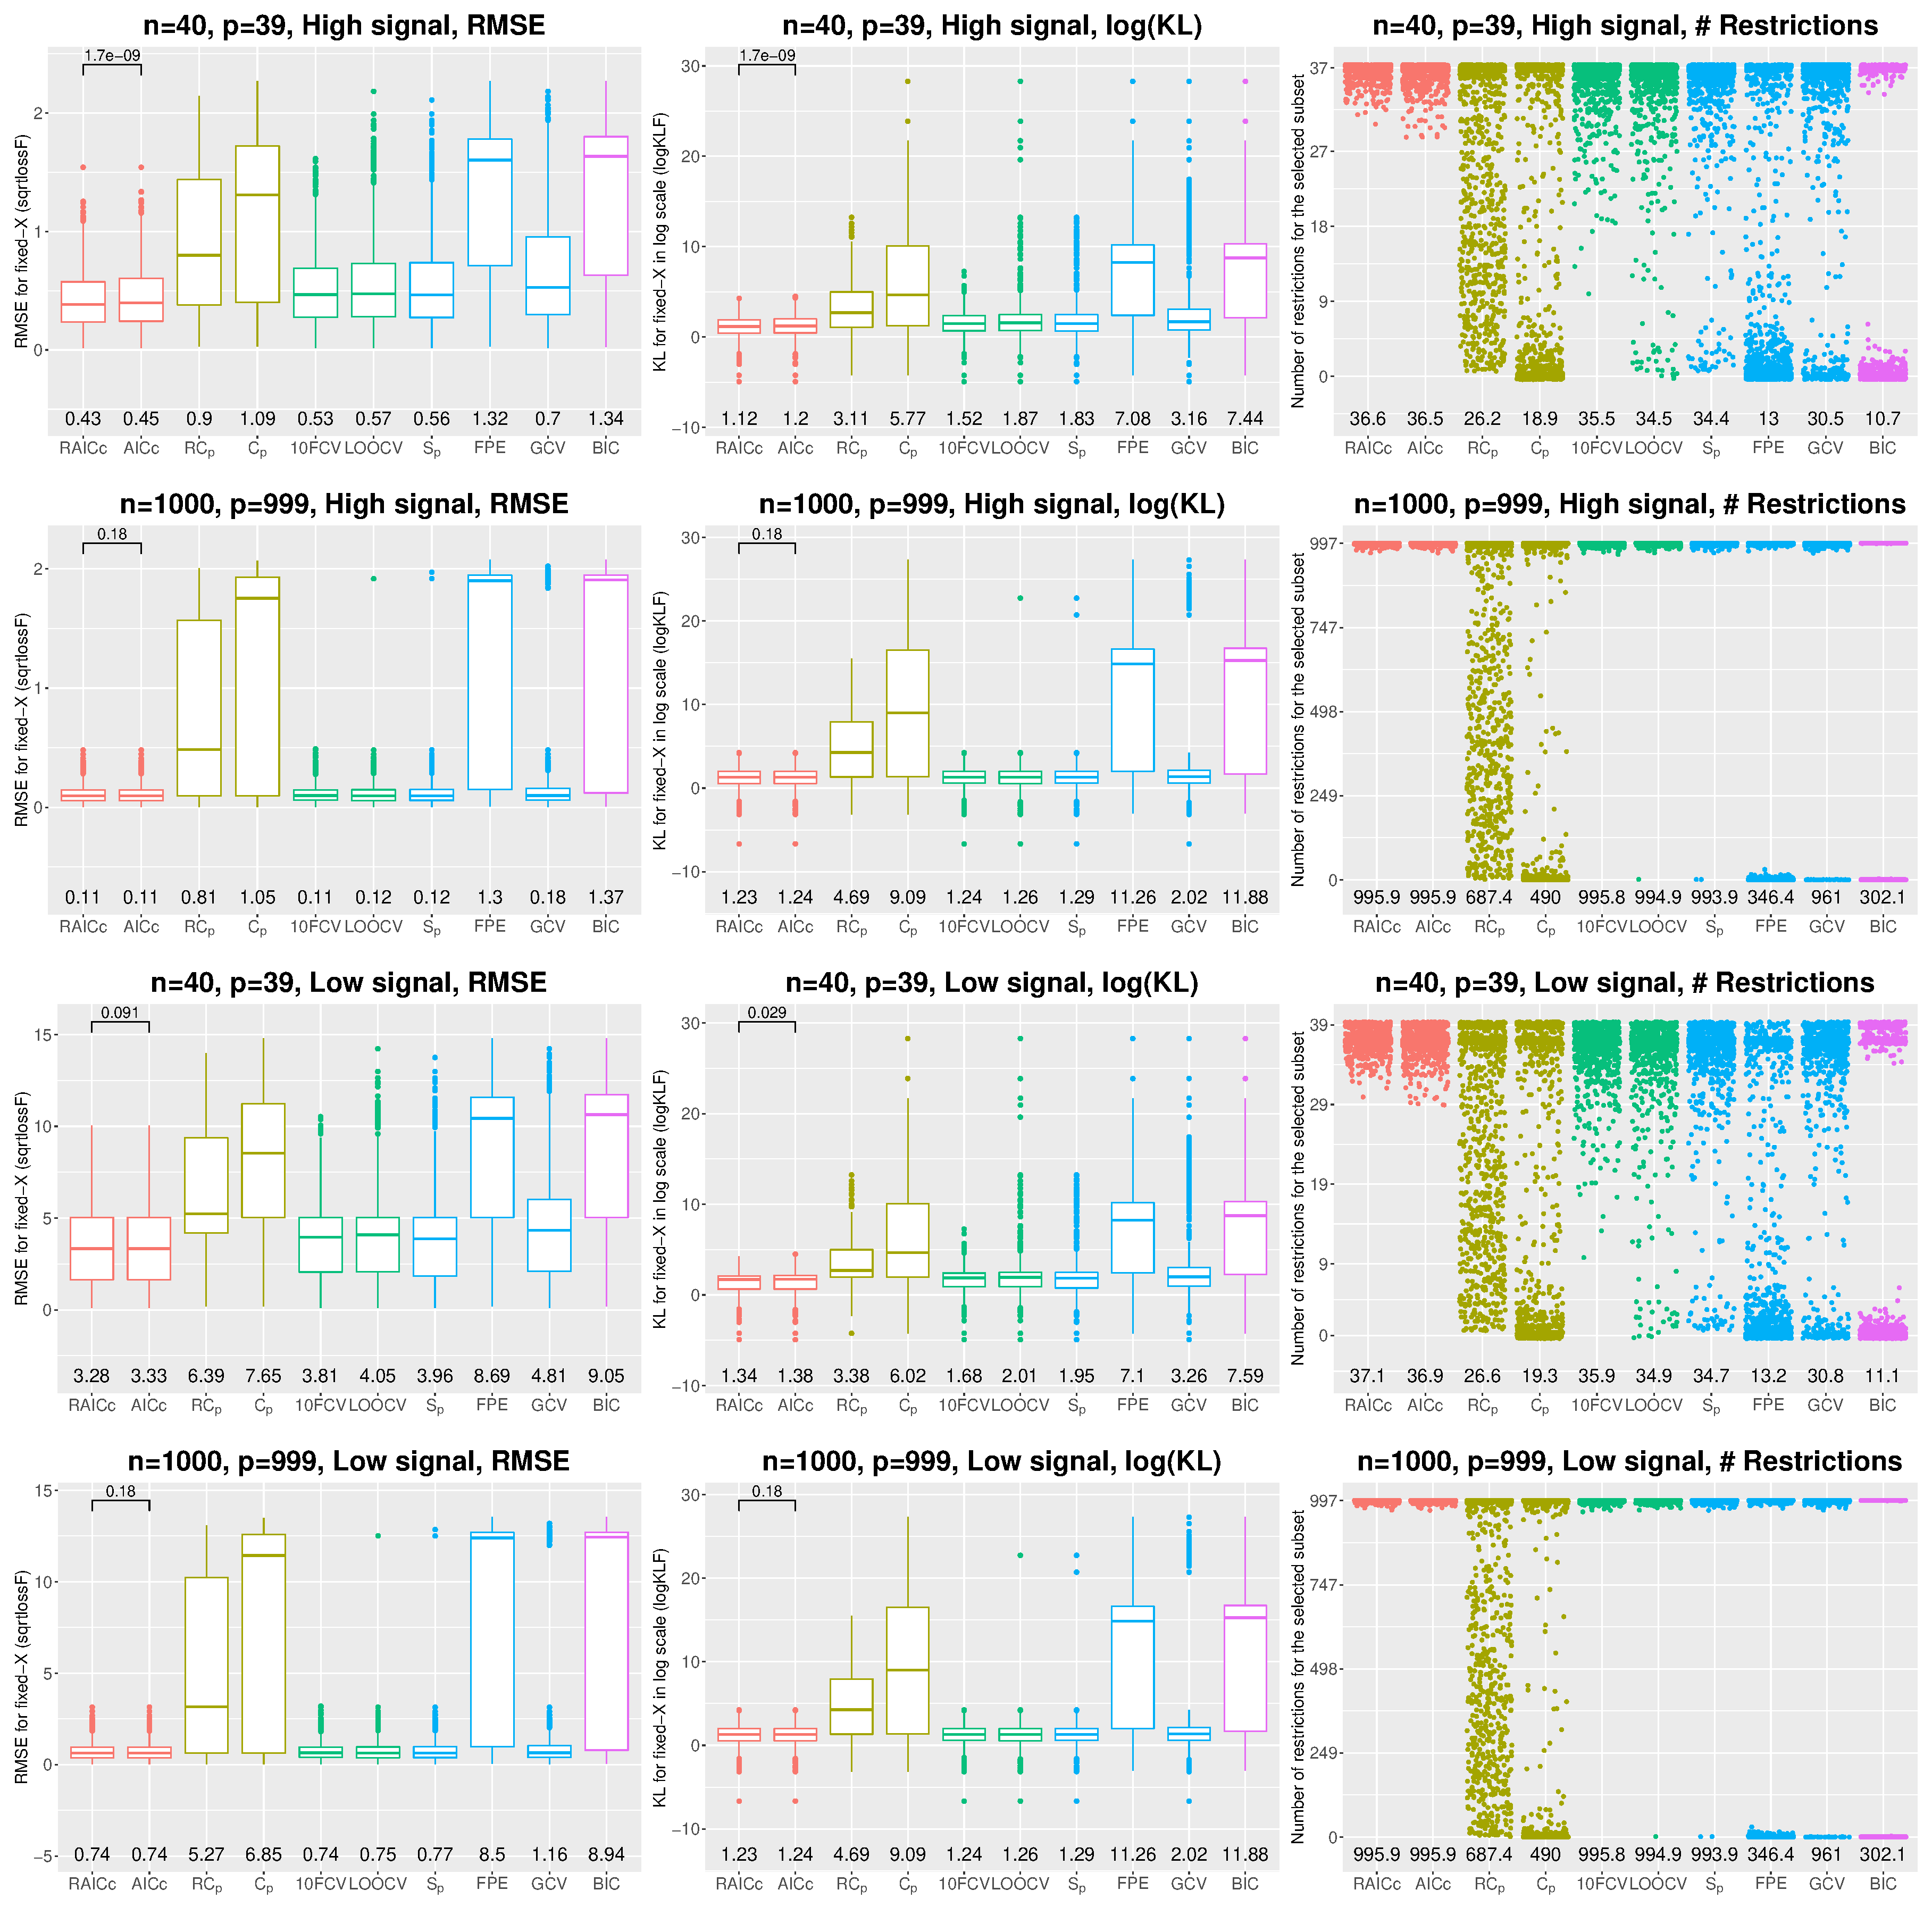
\includegraphics[width=\textwidth]{figures/main/fixedx_GR-Ex4.eps}
  \caption{Results of simulations for general restrictions. Fixed-X, GR-Ex4, $\rho=0.5$. The configurations are the same as in Figure \ref{fig:subsetgeneral_randomx}.}
  \label{fig:subsetgeneral_fixedx}
\end{figure}
%!TEX root = ms.tex
\section{Conclusion and future work}
\label{sec:conclusion}
In this paper, the use of information criteria to compare regression models under general linear restrictions for both fixed and random predictors is discussed. It is shown that general versions for KL-based discrepancy (AICc and RAICc, respectively) and squared error-based discrepancy (C$_p$ and RC$_p$, respectively) can be formulated as effectively unbiased estimators of predictive error (up to some terms that are free of the linear restrictions and hence are irrelevant when comparing criteria for different models). Model comparison based on the KL-based discrepancy measures are shown via simulations to be better-behaved than squared error-based discrepancies (including cross-validation) in selecting models with low predictive error.

The study of RAICc for variable selection in this paper focuses on OLS fits on pre-fixed predictors (e.g. nested predictors based on their physical orders in $X$). The discussion can be extended to other fitting procedures where the predictors in each subset are decided in a data-dependent way. For instance, \citet{tian2019use} discussed using AICc for best subset regression, and extending those results to the random-X scenario is a topic for future work. 

Note also that only restrictions on the regression coefficients are considered here, corresponding to restrictions on the regression portion of the model. It is also possible that the data analyst could be interested in restrictions on the distributional parameters of the predictors (restricting the variances of some predictors to be equal to each other, for example, or restricting covariances to follow a specified pattern such as autoregressive of order $1$ or compound symmetry), and it would be interesting to try to generalize the criteria discussed here to that situation.

\clearpage
\bibliographystyle{chicago}
%\bibliographystyle{natbib}

\bibliography{raicc.bib}

%!TEX root = ms.tex
\beginsupplement
\appendix
\pagenumbering{arabic}
\begin{center}
\textbf{\large Supplemental Material \\
Selection of Regression Models under Linear Restrictions \\ for Fixed and Random Designs}

Sen Tian, Clifford M. Hurvich, Jeffrey S. Simonoff
\end{center}

This document provides theoretical details of the theorems and lemmas in the paper. The complete simulation results and the computer code to reproduce the results can be viewed online\footnote{\url{https://github.com/sentian/RAICc}}.




\section{Proof of Lemma \ref{thm:components_ekl_lr_fixedx}}
\begin{proof}
As is well known \citeponline[see, e.g.,][p.~122]{greene2003econometric},
\begin{equation}
  n\hat\sigma^2 = \lVert y-X\hat{\beta} \rVert_2^2 \sim \sigma_0^2 \chi^2(n-p+m),
  \label{eq:dist_rss}
\end{equation}
and by using Assumption \ref{assumption}
\begin{equation}
\begin{aligned}
E_y\left(\hat{\beta} - \beta_0 \right) &= 0,\\
\text{Cov}_y\left(\hat{\beta} - \beta_0 \right) &= E\left[\left(\hat{\beta} - \beta_0 \right)\left(\hat{\beta} - \beta_0 \right)^T \right]\\
&= \sigma_0^2 \left\{ (X^T X)^{-1} - (X^T X)^{-1}R^T\left[ R(X^T X)^{-1}R^T \right]^{-1} R(X^T X)^{-1} \right\}.
\end{aligned}
\label{eq:dist_betahat}
\end{equation}
From \eqref{eq:dist_rss}, $1/\hat{\sigma}^2$ follows an inverse $\chi^2$ distribution and we have
\begin{equation*}
n \sigma_0^2 E_y\left[ \frac{1}{\hat{\sigma}^2} \right] = n\frac{n}{n-p+m-2}.
\end{equation*}
From \eqref{eq:dist_betahat}, we have
\begin{equation*}
E_y  \left [ (\hat \beta-\beta_0)^T X^T X (\hat \beta-\beta_0) \right ] 
= \text{Tr} \left[ X^T X \cdot \text{Cov}_y \left( \hat{\beta} - \beta_0 \right) \right]
= \sigma_0^2 (p-m).
\end{equation*}
We next show that $\hat{\sigma}^2$ and $(\hat \beta-\beta_0)^T X^T X (\hat \beta-\beta_0)$ are independent. Define the idempotent matrix $H_R=(X^T X)^{-1} R^T \left[ R (X^T X)^{-1} R^T \right]^{-1} R$. Recall that two other idempotent matrices are defined as $H=X(X^T X)^{-1} X^T$ and $H_Q = X H_R (X^T X)^{-1} X^T$, respectively. We have
\begin{equation*}
\begin{aligned}
y-X\hat{\beta}^f &= (I-H)\epsilon,\\
X\hat{\beta}^f - X\hat{\beta} &= XH_R(\hat{\beta}^f - \beta_0) =H_Q \epsilon,\\
X\hat{\beta} - X\beta_0 &= X(I-H_R)(\hat{\beta}^f - \beta_0) = (H-H_Q) \epsilon,
\end{aligned}
\end{equation*}
where we use the fact that $\hat{\beta}^f - \beta_0 = (X^T X)^{-1}X^T \epsilon$. Also since $HH_Q=H_QH=H_Q$, any two of the three idempotent symmetric matrices $I-H$, $H_Q$ and $H-H_Q$ have product zero. Then by Craig's Theorem \citeponline{craig1943note} on the independence of two quadratic forms in a normal vector, 
\begin{equation*}
n\hat{\sigma}^2 = \lVert y-X\hat{\beta} \rVert_2^2 = \lVert y-X\hat{\beta}^f \rVert_2^2 + \lVert X\hat{\beta}^f - X\hat{\beta} \rVert_2^2 = \epsilon^T (I-H) \epsilon + \epsilon^T H_Q \epsilon
\end{equation*}
and
\begin{equation*}
\lVert X\hat{\beta} - X\beta_0 \rVert_2^2 = \epsilon^T (H-H_Q) \epsilon
\end{equation*}
are independent.
\end{proof}


\section{Proof of Theorem \ref{thm:EoptF_KL}}
\begin{proof}
By using Lemma \ref{thm:components_ekl_lr_fixedx}, the expected KL discrepancy can be derived as
\begin{equation*}
\begin{aligned}
E_y [\text{ErrF}_\text{KL} ] 
&= E_y \left\{ n \log (2\pi \hat\sigma^2) + \frac{1}{\hat\sigma^2}  (\hat\beta-\beta_0)^T X^T X (\hat\beta-\beta_0) + \frac{n\sigma_0^2}{\hat\sigma^2} \right\} \\
&= E_y \left [ n\log (2\pi \hat \sigma^2)\right ] +  (p-m) \frac{n}{n-p+m-2} + n \frac{n}{n-p+m-2}\\
&= E_y \left [ n\log (2\pi \hat \sigma^2) \right ] +  n \frac{n+p-m}{n-p+m-2}.
\end{aligned}
\end{equation*}
Recall that
\begin{equation*}
\text{errF}_\text{KL} = n\log(2\pi \hat\sigma^2) + n.
\end{equation*}
The expected optimism is then
\begin{equation*}
E_y(\text{optF}_\text{KL}) = E_y[\text{ErrF}_\text{KL} ]  -  E_y[\text{errF}_\text{KL} ] = n \frac{n+p-m}{n-p+m-2} - n.
\end{equation*}
\end{proof}

\section{Proof of Theorem \ref{thm:EoptF_SE}}
\begin{proof}
Using the expression of $\hat\beta$ \eqref{eq:betahat_sigmahatsq} and the definitions of $H$ and $H_Q$, we have
\begin{equation*}
\hat{\mu} = X\hat{\beta} = (H-H_Q)y + X(X^T X)^{-1} R^T \left[ R(X^TX)^{-1}R^T  \right]^{-1}r,
\end{equation*}
where the second term on the right-hand side is deterministic. Denote $h_i$ and ${h_Q}_i$ as the $i$-th rows of $H$ and $H_Q$, respectively. We then have
\begin{equation*}
\text{Cov}_y \left(\hat{\mu}_i, y_i \right) = \text{Cov}_y \left[ (h_i-{h_Q}_i)y, y_i  \right] = \text{Cov}_y \left[ (H_{ii}-{H_Q}_{ii})y_i, y_i \right] = \sigma_0^2 (H_{ii}-{H_Q}_{ii}).
\end{equation*}
Therefore, the covariance penalty \eqref{eq:EoptF_SE} can be derived as
\begin{equation*}
E_y (\text{optF}_\text{SE}) = 2 \sum_{i=1}^n \text{Cov}_y (\hat\mu_i,y_i) = 2 \sigma_0^2 \text{Tr}(H-H_Q) = 2 \sigma_0^2 (p-m).
\end{equation*}
\end{proof}

\section{Proof of Lemma \ref{thm:components_ekl_lr_randomx}}
\begin{proof}
Since $x_i$ are iid $\mathcal{N}(0,\Sigma_0)$, $X^T X \sim \mathcal{W}(\Sigma_0, n)$ and $ (X^T X)^{-1} \sim \mathcal{W}^{-1} (\Sigma_0^{-1}, n)$, where $\mathcal{W}$ and $\mathcal{W}^{-1}$ denotes a Wishart and an inverse Wishart distribution with $n$ degrees of freedom, respectively. We have $E(X^T X) = n\Sigma_0$ and $E((X^T X)^{-1}) = \Sigma_0^{-1} / (n-p-1)$. Hence,
\begin{equation*}
  E \left[ \text{Tr}(\hat \Sigma^{-1}\Sigma_0) \right] = E \left[ \text{Tr} (n (X^T X)^{-1} \Sigma_0) \right] = n \text{Tr}\left[ E\left( (X^T X)^{-1} \right) \Sigma_0\right] = \frac{np}{n-p-1}.
\end{equation*}
Define $H_S = X(X^T X)^{-1}(I-H_R)^T \Sigma_0 (I-H_R) (X^T X)^{-1} X^T$. Conditionally on $X$, the random variable $\hat{\sigma}^2$ and 
\begin{equation*}
(\hat{\beta}-\beta_0)^T \Sigma_0 (\hat{\beta}-\beta_0) = \epsilon^T H_S \epsilon
\end{equation*}
are independent by Craig's Theorem, since $H_S$ is symmetric and $H_S(I-H+H_Q)=0$. 
\iffalse
We also have
\begin{equation*}
n\sigma_0^2 E_{X,y} \left[ \frac{1}{\hat\sigma^2} \right] = n\sigma_0^2 E_X\left[ E_y \left(\frac{1}{\hat\sigma^2}\big| X \right) \right] = n \frac{n}{n-p+m-2},
\end{equation*}
where the last equality we use the result in Lemma \ref{thm:components_ekl_lr_fixedx}. 
\fi
In order to calculate $\displaystyle E_{X,y}  \left [ (\hat \beta-\beta_0)^T \Sigma_0 (\hat \beta-\beta_0) \right ]$, we transform the original basis of the problem. Denote $\tilde{R} = \big(\begin{smallmatrix}
  R\\
  R^c
\end{smallmatrix}\big)$, a ($p \times p$) matrix, where the rows of $R^c$ span the orthogonal complement of the row space of $R$. Hence $\tilde{R}$ has full rank. The true model now becomes
\begin{equation*}
y = X \beta_0 + \epsilon = \tilde{X} \tilde{\beta}_0 + \epsilon,
\end{equation*}
where $\tilde{X} = X \tilde{R}^T$, $\tilde{\beta}_0 = \tilde{R}^{T^{-1}} \beta_0$. Denote $\tilde{M} = R \tilde{R}^T$. Assumption \ref{assumption} indicates that the true model in the new basis satisfies $\tilde{M} \tilde{\beta}_0 = r$. The approximating model is
\begin{equation*}
y = X \beta + u = \tilde{X} \tilde{\beta} + u,
\end{equation*}
with restrictions $\tilde{M} \tilde{\beta} = r$ where $\tilde{\beta} = \tilde{R}^{T^{-1}} \beta$. Denote $\hat{\tilde{\beta}}^f = (\tilde{X}^T \tilde{X})^{-1}\tilde{X}^Ty$ as the OLS estimator in the regression of $y$ on $\tilde{X}$. The restricted MLE is then
\begin{equation*}
\hat{\tilde{\beta}} = \hat{\tilde{\beta}}^f - \left( \tilde{X}^T \tilde{X} \right)^{-1} \tilde{M}^T \left[ \tilde{M} (\tilde{X}^T \tilde{X})^{-1} \tilde{M}^T \right]^{-1} \left( \tilde{M} \hat{\tilde{\beta}}^f - r \right),
\end{equation*}
and it can be easily verified that $\hat{\tilde{\beta}} = \tilde{R}^{T^{-1}} \hat{\beta}$. Denote $\tilde{X}_m$ and $\tilde{X}_{p-m}$ as the matrices containing the first $m$ and last $p-m$ columns of $\tilde{X}$, respectively. Let $\hat{\tilde{\beta}}_{m}$ and $\hat{\tilde{\beta}}_{p-m}$ be column vectors consisting of the first $m$ and last $p-m$ entries in $\hat{\tilde{\beta}}$, respectively. Also let $\tilde{\beta}_{0,m}$ and $\tilde{\beta}_{0,p-m}$ be column vectors consisting of the first $m$ and last $p-m$ entries in $\tilde{\beta}_0$, respectively. By using the formula for the inverse of partitioned matrices and some algebra, it can be shown that (details are given in Supplemental Material Section \ref{sec:derivation_betahattilde})
\begin{equation}
\begin{aligned}
\hat{\tilde{\beta}}_m &= \tilde{r},\\
\hat{\tilde{\beta}}_{p-m} &= \left( \tilde{X}_{p-m}^T \tilde{X}_{p-m} \right)^{-1} \left( \tilde{X}_{p-m}^Ty - \tilde{X}_{p-m}^T\tilde{X}_{m}\tilde{r} \right),
\end{aligned}
\label{eq:betahat_tilde_partition}
\end{equation}
where $\tilde{r} = (R R^T)^{-1}r$. The restrictions $\tilde{M}\tilde{\beta}_0=r$ results in $\tilde{\beta}_{0,m} = \tilde{r}$. We then have 
\begin{equation*}
\hat{\tilde{\beta}}_{p-m} - \tilde{\beta}_{0,p-m} = \left( \tilde{X}_{p-m}^T \tilde{X}_{p-m} \right)^{-1} \tilde{X}_{p-m} ^T \epsilon,
\end{equation*}
and therefore 
\begin{equation*}
\hat{\tilde{\beta}}_{p-m} - \tilde{\beta}_{0,p-m} \big | \tilde{X} \sim \mathcal{N} \left(0, \sigma_0^2 \left( \tilde{X}_{p-m}^T \tilde{X}_{p-m} \right)^{-1} \right).
\end{equation*}
We also note that $\tilde{X}_{p-m} = X {R^c}^T$, and hence the rows $\tilde{x}_{p-m, i}$ of $\tilde{X}_{p-m}$, are independent and satisfy $\tilde{x}_{p-m, i} \sim \mathcal{N} \left( 0, R^c \Sigma_0 {R^c}^T \right)$. We then have that $\left( \tilde{X}_{p-m}^T \tilde{X}_{p-m} \right)^{-1}$ follows the inverse Wishart distribution $W^{-1}( R^c \Sigma_0 {R^c}^T, n)$. The expectation of the quadratic form can be derived as
\begin{equation*}
\begin{aligned}
E_{X,y}  \left [ (\hat \beta-\beta_0)^T \Sigma_0 (\hat \beta-\beta_0) \right ] 
&=  E_{\tilde{X},y}  \left [ \left( \hat{\tilde{\beta}} - \tilde{\beta}_0 \right)^T \tilde{R} \Sigma_0 \tilde{R}^T \left( \hat{\tilde{\beta}} - \tilde{\beta}_0 \right) \right ]\\
&=  E_{\tilde{X}} \left\{ E  \left [ \left( \hat{\tilde{\beta}}_{p-m} - \tilde{\beta}_{0,p-m} \right)^T R^c \Sigma_0 {R^c}^T \left(\hat{\tilde{\beta}}_{p-m} - \tilde{\beta}_{0,p-m} \right) \Big| \tilde{X} \right ]  \right\}\\
&= \sigma_0^2 \text{Tr} \left\{ R^c \Sigma_0 {R^c}^T E \left[ \left( \tilde{X}_{p-m}^T \tilde{X}_{p-m} \right)^{-1} \right] \right\} \\
&= \sigma_0^2 \frac{p-m}{n-p+m-1}.
\end{aligned}
\end{equation*}

\end{proof}


\section{Proof of Theorem \ref{thm:EoptR_KL}}
\begin{proof}
The expected KL can be derived as
\begin{equation*}
\begin{aligned}
&E_{X,y} (\text{ErrR}_\text{KL}) \\
&= E_{X,y} \left [ n \log (2\pi \hat\sigma^2) + \frac{n}{\hat\sigma^2}  (\hat\beta-\beta_0)^T \Sigma_0 (\hat\beta-\beta_0) + \frac{n\sigma_0^2}{\hat\sigma^2} \right ] + E \left [np \log(2\pi) + n \log |\hat\Sigma| + n \text{Tr}(\hat\Sigma^{-1}\Sigma_{0}) \right] \\
&= E_{X,y} \left [ n \log (2\pi \hat\sigma^2) \right ] + E_X \left[E\left(\frac{n}{\hat\sigma^2} \big | X \right)  E\left((\hat\beta-\beta_0)^T \Sigma_0 (\hat\beta-\beta_0) \big| X \right) + E\left(\frac{n\sigma_0^2}{\hat\sigma^2} \big| X \right) \right] + \\
 & \qquad E \left [np \log(2\pi) + n \log |\hat\Sigma| + n \text{Tr}(\hat\Sigma^{-1}\Sigma_{0}) \right] \\
&= E_{X,y} \left [ n\log (2\pi \hat \sigma^2) \right ] +  n \frac{n(n-1)}{(n-p+m-2)(n-p+m-1)} + E \left [ n\log |\hat \Sigma| \right ] + np\log(2\pi) + n \frac{np}{n-p-1},
\end{aligned}
\end{equation*}
where the second equality is based on Lemma \ref{thm:components_ekl_lr_randomx} for the independence of $\hat\sigma^2$ and $(\hat\beta-\beta_0)^T \Sigma_0 (\hat\beta-\beta_0)$ conditionally on $X$, and in the last equality we use results from Lemmas \ref{thm:components_ekl_lr_fixedx} and \ref{thm:components_ekl_lr_randomx}. Since the training error is
\begin{equation*}
\text{errR}_\text{KL} = -2\log L(\hat\beta,\hat\sigma^2,\hat\Sigma|X,y) = \left [ n \log (2\pi \hat\sigma^2) + n \right ] + \left [np \log(2\pi) + n \log |\hat\Sigma| + np \right ],
\end{equation*}
the expected optimism can be obtained as
\begin{equation*}
\begin{aligned}
E_{X,y}(\text{optR}_\text{KL}) 
&= E_{X,y}[\text{ErrR}_\text{KL} ]  -  E_{X,y}[\text{errR}_\text{KL} ] \\
&= n \frac{n(n-1)}{(n-p+m-2)(n-p+m-1)} + n \frac{np}{n-p-1} - n(p+1).
\end{aligned}
\end{equation*}
\end{proof}


\section{Proof of Theorem \ref{thm:EoptR_SE}}
\begin{proof}

We first note from Theorem \ref{thm:EoptF_SE} that
\begin{equation*}
E_{X,y}(\text{optF}_\text{SE}) = E \left[ E(\text{optF}_\text{SE} | X ) \right] = 2 \sigma_0^2(p-m).
\end{equation*}
Based on formula 6 and proposition 1 in \citetonline{rosset2020fixed}, the expected optimism can be decomposed into 
\begin{equation*}
E_{X,y}(\text{optR}_\text{SE}) = E_{X,y}(\text{optF}_\text{SE}) + B^+ + V^+ = 2 \sigma_0^2(p-m) +  B^+ + V^+,
\end{equation*}
where $B^+$ and $V^+$ are the excess bias and excess variance of the fit. In particular, the excess bias is defined as
\begin{equation*}
B^+ = E_{X,X^{(n)}} \big\lVert E( X^{(n)} \hat{\beta} \big | X, X^{(n)} ) - X^{(n)} \beta_0 \big\rVert_2^2 - E_X \big\lVert E( X \hat{\beta} \big | X ) - X \beta_0 \big\rVert_2^2.
\end{equation*}
Because of Assumption \ref{assumption} that the true model satisfies the restrictions, it follows that $\hat{\beta}$ is unbiased, and hence it is easy to see that $B^+=0$. Next, $V^+$ is defined as
\begin{equation*}
V^+ = E_{X,X^{(n)}} \left\{ \text{Tr} \left[ \text{Cov}\left( X^{(n)}\hat{\beta} \big | X, X^{(n)} \right) \right] \right\} - E_X \left\{ \text{Tr} \left[ \text{Cov}\left( X\hat{\beta} \big | X \right)  \right] \right\}.
\end{equation*}
The second term on the right-hand side is
\begin{equation*}
E_X \left\{  \text{Tr} \left[ \text{Cov} \left( X\hat{\beta} \big | X \right)  \right] \right\} = E_X \left\{ \text{Tr} \left[ \text{Cov} \left( (H-H_Q)y \big | X \right)  \right] \right\} = E\left\{  \sigma_0^2 \text{Tr} \left( H-H_Q  \right) \right\}= \sigma_0^2 (p-m).
\end{equation*}
The first term on the right-hand side is
\begin{equation*}
\begin{aligned}
& E_{X,X^{(n)}} \text{Tr} \left[ \text{Cov}\left( X^{(n)}\hat{\beta} \big | X, X^{(n)} \right) \right] \\
&= E_{X,X^{(n)}} \text{Tr} \left[ \text{Cov} \left( X^{(n)} (\hat{\beta} -\beta_0) \big | X, X^{(n)} \right) \right] \\
&= \text{Tr} \left\{ E_X\left[ \text{Cov} \left( \hat{\beta} -\beta_0 \big | X \right) \right] E \left ({X^{(n)}}^T X^{(n)}) \right] \right\}\\
&= n E_X \left\{ \text{Tr} \left[ \Sigma_0 \text{Cov} \left( \hat{\beta} - \beta_0  \big | X \right) \right] \right\}\\
&= n E_X \left\{ E\left[ \left(\hat{\beta} - \beta_0 \right)^T \Sigma_0 \left(\hat{\beta} - \beta_0 \right) \big| X \right] \right\} \\
&= n E_{X,y} \left[ \left(\hat{\beta} - \beta_0 \right)^T \Sigma_0 \left(\hat{\beta} - \beta_0 \right) \right]\\
&= n \sigma_0^2 \frac{p-m}{n-p+m-1},
\end{aligned}
\end{equation*}
where in the third equality we use the independence and identical distribution of $X$ and $X_0$, and $E(X^T X) = n\Sigma_0$, while in the last equality we use the result in Lemma \ref{thm:components_ekl_lr_randomx}. Combining the results together, we have
\begin{equation*}
V^+ = n\sigma_0^2 \frac{p-m}{n-p+m-1} - \sigma_0^2 (p-m) = \sigma_0^2\frac{(p-m)(p-m+1)}{n-p+m-1},
\end{equation*}
and 
\begin{equation*}
E_{X,y}(\text{optR}_\text{SE}) = 2\sigma_0^2 (p-m) + \sigma_0^2\frac{(p-m)(p-m+1)}{n-p+m-1}.
\end{equation*}

\end{proof}

\section{Derivation of the expression of \texorpdfstring{$\hat{\tilde{\beta}}$}{} in \eqref{eq:betahat_tilde_partition} }
\label{sec:derivation_betahattilde}

Denote $\tilde{H}_m = \tilde{X}_m \left(\tilde{X}_m^T \tilde{X}_m \right)^{-1} \tilde{X}_m^T$ and $\tilde{H}_{p-m} = \tilde{X}_{p-m} \left(\tilde{X}_{p-m}^T \tilde{X}_{p-m}\right)^{-1} \tilde{X}_{p-m}^T$. Then the partitioned form of the matrix $\tilde{X}^T \tilde{X}$ is given by
\begin{equation*}
\begin{aligned}
& \left(\tilde{X}^T \tilde{X}\right)^{-1} = 
\begin{bmatrix}
\tilde{X}_m^T \tilde{X}_m & \tilde{X}_m^T \tilde{X}_{p-m} \\
\tilde{X}_{p-m}^T \tilde{X}_m & \tilde{X}_{p-m}^T \tilde{X}_{p-m}
\end{bmatrix}^{-1} \\
&=
\begin{bmatrix}
\left[\tilde{X}_m^T (I-\tilde{H}_{p-m}) \tilde{X}_m \right]^{-1} & - \left[\tilde{X}_m^T (I-\tilde{H}_{p-m}) \tilde{X}_m \right]^{-1} \tilde{X}_m^T \tilde{X}_{p-m} \left(\tilde{X}_{p-m}^T \tilde{X}_{p-m}\right)^{-1}\\
- \left[\tilde{X}_{p-m}^T \left(I-\tilde{H}_m\right) \tilde{X}_{p-m} \right]^{-1} \tilde{X}_{p-m}^T \tilde{X}_m \left(\tilde{X}_m^T \tilde{X}_m \right)^{-1} & \left[\tilde{X}_{p-m}^T \left(I-\tilde{H}_m\right) \tilde{X}_{p-m} \right]^{-1}
\end{bmatrix},
\end{aligned}
\end{equation*}
and the partitioned form of $\hat{\tilde{\beta}}^f$ is given by
\begin{equation*}
\begin{aligned}
\hat{\tilde{\beta}}^f &= \left(\tilde{X}^T \tilde{X}\right)^{-1} \tilde{X}^T y \\
&= 
\begin{bmatrix}
\left[\tilde{X}_m^T \left(I-\tilde{H}_{p-m}\right) \tilde{X}_m \right]^{-1} \left( \tilde{X}_m^T y - \tilde{X}_m^T \tilde{H}_{p-m} y \right) \\
\left[\tilde{X}_{p-m}^T \left(I-\tilde{H}_m\right) \tilde{X}_{p-m} \right]^{-1} \left( \tilde{X}_{p-m}^T y - \tilde{X}_{p-m}^T \tilde{H}_m y \right)
\end{bmatrix}.
\end{aligned}
\end{equation*}
We also have 
\begin{equation*}
\begin{aligned}
& \left[\tilde{X}_{p-m}^T \left(I-\tilde{H}_m\right) \tilde{X}_{p-m} \right]^{-1} \tilde{X}_{p-m}^T \tilde{H}_m \left(I_n - \tilde{H}_{p-m}\right)\tilde{X}_m \\
&= \left[\tilde{X}_{p-m}^T \left(I-\tilde{H}_m\right) \tilde{X}_{p-m} \right]^{-1} \left( \tilde{X}_{p-m}^T \tilde{X}_m - \tilde{X}_{p-m}^T \tilde{H}_m\tilde{H}_{p-m}\tilde{X}_m \right)  \\
&= \left[\tilde{X}_{p-m}^T \left(I-\tilde{H}_m\right) \tilde{X}_{p-m} \right]^{-1} \tilde{X}_{p-m}^T \left(I-\tilde{H}_m\right) \tilde{X}_{p-m} \left(\tilde{X}_{p-m}^T \tilde{X}_{p-m} \right)^{-1} \tilde{X}_{p-m}^T \tilde{X}_m  \\
&= \left(\tilde{X}_{p-m}^T \tilde{X}_{p-m} \right)^{-1} \tilde{X}_{p-m}^T \tilde{X}_m.
\end{aligned}
\end{equation*}
Using this property and $\tilde{M} = R \tilde{R}^T = \big(\begin{smallmatrix}
  RR^T & 0
\end{smallmatrix}\big)$, we have
\begin{equation*}
\begin{aligned}
\left(\tilde{X}^T \tilde{X}\right)^{-1} \tilde{M}^T \left[ \tilde{M} \left( \tilde{X}^T \tilde{X} \right)^{-1} \tilde{M}^T \right]^{-1} &= 
\begin{bmatrix}
(RR^T)^{-1} \\
-\left(\tilde{X}_{p-m}^T \tilde{X}_{p-m} \right)^{-1} \tilde{X}_{p-m}^T \tilde{X}_m (RR^T)^{-1}
\end{bmatrix},
 \\ 
I_p - \left(\tilde{X}^T \tilde{X}\right)^{-1} \tilde{M}^T \left[ \tilde{M} \left( \tilde{X}^T \tilde{X} \right)^{-1} \tilde{M}^T \right]^{-1} \tilde{M} &= 
\begin{bmatrix}
0 & 0\\
\left(\tilde{X}_{p-m}^T \tilde{X}_{p-m} \right)^{-1} \tilde{X}_{p-m}^T \tilde{X}_m & I_{p-m}
\end{bmatrix}.
\end{aligned}
\end{equation*}
Therefore, \eqref{eq:betahat_tilde_partition} can be derived as
\begin{equation*}
\begin{aligned}
\hat{\tilde{\beta}} &= \left\{I_p - \left(\tilde{X}^T \tilde{X}\right)^{-1} \tilde{M}^T \left[ \tilde{M} \left( \tilde{X}^T \tilde{X} \right)^{-1} \tilde{M}^T \right]^{-1} \tilde{M} \right\}\hat{\tilde{\beta}}^f + \left\{\left(\tilde{X}^T \tilde{X}\right)^{-1} \tilde{M}^T \left[ \tilde{M} \left( \tilde{X}^T \tilde{X} \right)^{-1} \tilde{M}^T \right]^{-1} \right\}r\\
&=
\begin{bmatrix}
\tilde{r}\\
\left(\tilde{X}_{p-m}^T \tilde{X}_{p-m} \right)^{-1} \tilde{X}_{p-m}^T \left(y - \tilde{X}_m \tilde{r}\right)
\end{bmatrix}.
\end{aligned}
\end{equation*}


\iffalse
\section{\texorpdfstring{$\hat{\beta}$}{} for \texorpdfstring{$R=[0, I_{p-k}]$}{} }
We show that for $R=[0, I_{p-k}]$, $\hat{\beta}$ \eqref{eq:betahat} is the least squares coefficient vector of $y$ upon $X_k$ where $X_k$ involves the first $k$ columns of $X$. 

We simplify the notations. Denote $R=[0, I_2]$ where $0$ is an $p_2 \times p_1$ matrix and $I_2$ is an $p_2 \times p_2$ matrix, respectively. Also denote $X=[X_1, X_2]$ where $X_1$ is an $n \times p_1$ matrix and $X_2$ is an $n \times p_2$ matrix, respectively. The corresponding hat matrices are $H_1 = X_1 (X_1^T X_1)^{-1} X_1^T$ and $H_2 = X_2 (X_2^T X_2)^{-1} X_2^T$. 

First note that the partitioned form of the matrix $X^T X$ is given by
\begin{equation}
\begin{aligned}
(X^T X)^{-1} &= 
\begin{bmatrix}
X_1^T X_1 & X_1^T X_2 \\
X_2^T X_1 & X_2^T X_2
\end{bmatrix}^{-1} \\
&=
\begin{bmatrix}
[X_1^T (I-H_2) X_1 ]^{-1} & - [X_1^T (I-H_2) X_1 ]^{-1} X_1^T X_2 (X_2^T X_2)^{-1}\\
- [X_2^T (I-H_1) X_2 ]^{-1} X_2^T X_1 (X_1^T X_1)^{-1} & [X_2^T (I-H_1) X_2 ]^{-1}
\end{bmatrix}.
\end{aligned}
\end{equation}
Then we have
\begin{equation*}
I - H_R=
I - (X^T X)^{-1}(R^T X_2^T (I-H_1) X_2 R) =
\begin{bmatrix}
I_1 & [X_1^T (I-H_2) X_1 ]^{-1} X_1^T H_2 (I-H_1) X_2 \\
0 & 0
\end{bmatrix},
\end{equation*}
and
\begin{equation*}
z = (X^T X)^{-1} X^T y = 
\begin{bmatrix}
[X_1^T (I-H_2) X_1 ]^{-1} (X_1^T y - X_1^T H_2 y)\\
[X_2^T (I-H_1) X_2 ]^{-1} (X_2^T y - X_2^T H_1 y)
\end{bmatrix}.
\end{equation*}
Also it can be easily verified that $HH_1=H_1H=H_1$, $HH_2=H_2H=H_2$, and
\begin{equation*}
(I-H_1)X_2 [X_2^T (I-H_1) X_2 ]^{-1} X_2^T (I-H_1) = H - H_1.
\end{equation*}
Therefore, we have
\begin{equation*}
\begin{aligned}
  \hat{\beta} &= z + (X^T X)^{-1} R^T ( R(X^T X)^{-1} R^T)^{-1} (r-R z) \\
  &= \left[ I
   - (X^T X)^{-1}(R^T X_2^T (I-H_1) X_2 R) \right] z\\
  &= [X_1^T (I-H_2) X_1 ]^{-1} X_1^T \left\{ I-H_2+H_2(I-H_1)X_2 [X_2^T (I-H_1) X_2 ]^{-1} X_2^T (I-H_1)  \right\}y \\
  &= [X_1^T (I-H_2) X_1 ]^{-1} X_1^T \left\{ I-H_2H_1 \right\}y\\
  &= (X_1^T X_1)^{-1} X_1^T y,
\end{aligned}
\end{equation*}
which is the least squares estimates on $X_1$.

\section{Derivation of \texorpdfstring{\eqref{eq:firstterm_ekl_lr}}{} for \texorpdfstring{$R=[0, I_{p-k}]$}{}}
First note that
\begin{equation*}
\begin{aligned}
&[X_1^T (I-H_2) X_1 ]^{-1} - [X_1^T (I-H_2) X_1 ]^{-1} X_1^T H_2 (I-H_1) X_2 [X_2^T (I-H_1) X_2 ]^{-1} X_2^T X_1 (X_1^T X_1)^{-1}\\
&= [X_1^T (I-H_2) X_1 ]^{-1} \left( I - X_1^T H_2 X_1 (X_1^T X_1)^{-1} \right),\\
&= (X_1^T X_1)^{-1} 
\end{aligned}
\end{equation*}
Then from the partition of $(X^T X)^{-1}$ and the expression of $I-H_R$ shown in the above Section, it is easy to have
\begin{equation*}
(I-H_R) (X^T X)^{-1} = 
\begin{bmatrix}
(X_1^T X_1)^{-1}  & 0\\
0 & 0
\end{bmatrix}.
\end{equation*}
Therefore,
\begin{equation*}
\begin{aligned}
E_0  \left [ (\hat \beta-\beta_0)^T \Sigma_0 (\hat \beta-\beta_0) \right ] &= E_0 \left\{ E_0 \left [ (\hat \beta-\beta_0)^T \Sigma_0 (\hat \beta-\beta_0) \Big| X \right ]  \right\},\\
&= \sigma_0^2 \text{Tr} \left[ \Sigma_0 E_0 \left\{ (I-H_R) (X^T X)^{-1} \right\} \right], \\
&= \sigma_0^2 \frac{p_1}{n-p_1-1}.
\end{aligned}
\end{equation*}

\section{Cochrane's Theorem}
Let $\eta \sim \mathcal{N}(0, I)$ and let $H=\sum H_i$ be a sum of $k$ symmetric matrices with $\text{rank}(H)$=r and $\text{rank}(H_i)=r_i$ such that $H_i=H_i^2$ and $H_iH_j=0$ when $i \ne j$. Then $\eta^T H_i \eta \sim \chi^2(r_i)$, $i=1,\cdots,k$ are independent chi-square variates such that $\sum \eta^T H_i \eta = \eta^T H \eta \sim \chi^2(r)$ with $r=\sum r_i$.




\section{Using Adkin's result to derive \texorpdfstring{\eqref{eq:thirdterm_ekl_lr_randomx}}{} for any \texorpdfstring{$R$}{}}

\textcolor{red}{Unfinished}

The problem we have is 
\begin{equation}
y = X\beta_0 + \epsilon, \quad \text{s.t. } R\beta_0=r,
\end{equation}
where $R$ is a $m$ by $p$ matrix. From the eigen-decomposition of $X^T X$, we have $X^T X = P \Lambda P^T$. Denote $V = P \Lambda^{1/2} P^T$ and $V^{-1} = P \Lambda^{-1/2} P^T$. Also denote $H_1 = R V^{-1}$, and an orthogonal matrix $Q$ that contains the characteristic vectors of $H_1 ^T (H_1 H_1^T)^{-1} H_1$. Hence, $Z = XV^{-1}Q$ has orthonormal columns. Adkins shows that the problem can be transformed to
\begin{equation}
y = Z\theta_0 + \epsilon, \quad \text{s.t. } [I_m \quad 0]\theta_0=h,
\end{equation}
where $h$ is some constant. 

Denote $\hat{\theta}^f = Z^T y$ as the OLS estimator, 
\begin{equation}
\begin{aligned}
( \hat{\beta} - \beta_0 )^T \Sigma_0 ( \hat{\beta} - \beta_0 ) 
&= ( \hat{\theta} - \theta_0 )^T Q^T V^{-1} \Sigma_0 V^{-1} Q ( \hat{\theta} - \theta_0 ) \\
&= ( \hat{\theta}^f_{p-m} - \theta_{0,p-m} )^T [0 \quad I_{p-m}] Q^T V^{-1} \Sigma_0 V^{-1} Q [0 \quad I_{p-m}]^T ( \hat{\theta}^f_{p-m} - \theta_{0,p-m} ),
\end{aligned}
\end{equation}
where $\hat{\theta}^f_{p-m}$ is the last $p-m$ elements of $\hat{\theta}^f$ and $\theta_{0,p-m}$ is the last $p-m$ elements of $\theta_0$. Since $\hat{\theta}^f_{p-m} - \theta_{0,p-m} \sim \mathcal{N}(0, \sigma_0^2 I_{p-m})$, we have
\begin{equation}
\begin{aligned}
E_0 \left\{ ( \hat{\beta} - \beta_0 )^T \Sigma_0 ( \hat{\beta} - \beta_0 )  \right\} 
&= E_0 \left\{ E_0 \left[ ( \hat{\beta} - \beta_0 )^T \Sigma_0 ( \hat{\beta} - \beta_0 ) | X \right]  \right\},\\
&= \sigma_0^2 E_0\left\{ \text{Tr}\left( [0 \quad I_{p-m}] Q^T V^{-1} \Sigma_0 V^{-1} Q [0 \quad I_{p-m}]^T \right) \right\}
\end{aligned}
\end{equation}
Here $Q$ and $V$ are random. I verify in simulations that the matrix $E_0 ([0 \quad I_{p-m}] Q^T V^{-1} \Sigma_0 V^{-1} Q [0 \quad I_{p-m}]^T)$ is a diagonal matrix.
\fi


\bibliographystyleonline{chicago}
\bibliographyonline{raicc.bib}

\iffalse
% latex table generated in R 4.0.2 by xtable 1.8-4 package
% Fri Jun 26 10:43:44 2020
\begin{table}[ht]
\centering
\caption{Fixed X, Sparse-Ex1, n=40} 
\scalebox{0.52}{
\begin{tabular}{|c|c|c|cc|cc|cc|ccc|c||cc|cc|cc|ccc|c|}
  \toprule 
 \multicolumn{1}{|c}{} & \multicolumn{1}{c}{} &       & RAICc & AICc  & RC$_p$ & C$_p$ & 10F CV & LOO CV & S$_p$ & $\widehat{\text{C}}_p$ & GCV   & BIC   & RAICc & AICc  & RC$_p$ & C$_p$ & 10F CV & LOO CV & S$_p$ & $\widehat{\text{C}}_p$ & GCV   & BIC  \\
 \cmidrule{4-23}\multicolumn{1}{|c}{} & \multicolumn{1}{c}{} &       & \multicolumn{10}{c||}{RMSE}                                                   & \multicolumn{10}{c|}{Relative Risk}       \\
 \midrule\multirow{9}[6]{*}{hsnr} & \multirow{3}[2]{*}{$\rho=0$} & p=12 & 0.718 & 0.731 & 0.741 & 0.777 & 0.781 & 0.772 & 0.772 & 0.801 & 0.774 & 0.732 & 0.023 & 0.024 & 0.024 & 0.027 & 0.028 & 0.027 & 0.027 & 0.029 & 0.027 & 0.024 \\ 
   &  & p=20 & 0.718 & 0.733 & 0.758 & 0.826 & 0.808 & 0.805 & 0.804 & 0.891 & 0.808 & 0.741 & 0.023 & 0.024 & 0.026 & 0.036 & 0.032 & 0.032 & 0.032 & 0.045 & 0.032 & 0.025 \\ 
   &  & p=36 & 0.718 & 0.733 & 0.857 & 1.035 & 0.819 & 0.835 & 0.829 & 1.223 & 0.849 & 1.008 & 0.023 & 0.024 & 0.048 & 0.211 & 0.035 & 0.05 & 0.049 & 0.335 & 0.062 & 0.25 \\ 
  \cmidrule{2-23} & \multirow{3}[2]{*}{$\rho=0.5$} & p=12 & 1.118 & 1.129 & 1.138 & 1.169 & 1.164 & 1.167 & 1.156 & 1.198 & 1.158 & 1.14 & 0.024 & 0.025 & 0.026 & 0.027 & 0.027 & 0.027 & 0.027 & 0.029 & 0.027 & 0.025 \\ 
   &  & p=20 & 1.118 & 1.128 & 1.155 & 1.248 & 1.204 & 1.212 & 1.204 & 1.326 & 1.207 & 1.145 & 0.024 & 0.025 & 0.027 & 0.036 & 0.031 & 0.032 & 0.032 & 0.044 & 0.032 & 0.026 \\ 
   &  & p=36 & 1.118 & 1.128 & 1.3 & 1.554 & 1.22 & 1.249 & 1.236 & 1.803 & 1.264 & 1.507 & 0.024 & 0.025 & 0.048 & 0.203 & 0.034 & 0.049 & 0.047 & 0.317 & 0.061 & 0.232 \\ 
  \cmidrule{2-23} & \multirow{3}[2]{*}{$\rho=0.9$} & p=12 & 1.597 & 1.604 & 1.623 & 1.67 & 1.663 & 1.656 & 1.655 & 1.706 & 1.657 & 1.655 & 0.023 & 0.024 & 0.025 & 0.027 & 0.026 & 0.026 & 0.026 & 0.029 & 0.026 & 0.025 \\ 
   &  & p=20 & 1.564 & 1.569 & 1.608 & 1.737 & 1.676 & 1.68 & 1.671 & 1.849 & 1.677 & 1.629 & 0.022 & 0.023 & 0.025 & 0.036 & 0.03 & 0.03 & 0.03 & 0.043 & 0.03 & 0.025 \\ 
   &  & p=36 & 1.572 & 1.579 & 1.853 & 2.22 & 1.695 & 1.745 & 1.73 & 2.564 & 1.771 & 2.137 & 0.022 & 0.023 & 0.047 & 0.215 & 0.032 & 0.049 & 0.047 & 0.33 & 0.058 & 0.232 \\ 
  \midrule\multirow{9}[6]{*}{msnr} & \multirow{3}[2]{*}{$\rho=0$} & p=12 & 2.385 & 2.372 & 2.359 & 2.382 & 2.396 & 2.379 & 2.365 & 2.411 & 2.368 & 2.55 & 0.241 & 0.24 & 0.239 & 0.246 & 0.25 & 0.245 & 0.242 & 0.255 & 0.243 & 0.279 \\ 
   &  & p=20 & 2.385 & 2.373 & 2.393 & 2.51 & 2.448 & 2.454 & 2.43 & 2.634 & 2.44 & 2.561 & 0.241 & 0.241 & 0.253 & 0.316 & 0.277 & 0.283 & 0.274 & 0.376 & 0.278 & 0.285 \\ 
   &  & p=36 & 2.385 & 2.373 & 2.711 & 3.176 & 2.475 & 2.537 & 2.503 & 3.586 & 2.55 & 3.176 & 0.241 & 0.241 & 0.449 & 1.816 & 0.305 & 0.431 & 0.41 & 2.798 & 0.51 & 1.96 \\ 
  \cmidrule{2-23} & \multirow{3}[2]{*}{$\rho=0.5$} & p=12 & 3.339 & 3.336 & 3.346 & 3.393 & 3.386 & 3.372 & 3.351 & 3.434 & 3.351 & 3.521 & 0.211 & 0.213 & 0.215 & 0.225 & 0.223 & 0.222 & 0.219 & 0.233 & 0.219 & 0.237 \\ 
   &  & p=20 & 3.341 & 3.339 & 3.377 & 3.589 & 3.475 & 3.469 & 3.444 & 3.765 & 3.455 & 3.529 & 0.211 & 0.214 & 0.226 & 0.294 & 0.252 & 0.255 & 0.248 & 0.348 & 0.251 & 0.24 \\ 
   &  & p=36 & 3.341 & 3.339 & 3.842 & 4.573 & 3.506 & 3.564 & 3.54 & 5.177 & 3.624 & 4.434 & 0.211 & 0.214 & 0.408 & 1.717 & 0.271 & 0.387 & 0.376 & 2.643 & 0.482 & 1.8 \\ 
  \cmidrule{2-23} & \multirow{3}[2]{*}{$\rho=0.9$} & p=12 & 4.263 & 4.337 & 4.456 & 4.579 & 4.512 & 4.5 & 4.522 & 4.661 & 4.531 & 4.484 & 0.146 & 0.156 & 0.173 & 0.19 & 0.182 & 0.182 & 0.183 & 0.204 & 0.185 & 0.152 \\ 
   &  & p=20 & 4.162 & 4.249 & 4.42 & 4.775 & 4.511 & 4.538 & 4.535 & 5.018 & 4.568 & 4.378 & 0.142 & 0.154 & 0.18 & 0.259 & 0.201 & 0.211 & 0.205 & 0.308 & 0.21 & 0.15 \\ 
   &  & p=36 & 4.169 & 4.261 & 5.121 & 6.246 & 4.545 & 4.7 & 4.682 & 7.173 & 4.765 & 5.74 & 0.142 & 0.155 & 0.363 & 1.787 & 0.21 & 0.334 & 0.342 & 2.69 & 0.388 & 1.707 \\ 
  \midrule\multirow{9}[6]{*}{lsnr} & \multirow{3}[2]{*}{$\rho=0$} & p=12 & 4.563 & 4.621 & 4.686 & 4.834 & 4.746 & 4.756 & 4.757 & 4.911 & 4.766 & 4.881 & 0.807 & 0.842 & 0.893 & 0.983 & 0.931 & 0.934 & 0.938 & 1.024 & 0.944 & 0.897 \\ 
   &  & p=20 & 4.563 & 4.625 & 4.783 & 5.095 & 4.869 & 4.887 & 4.879 & 5.339 & 4.897 & 4.884 & 0.807 & 0.846 & 0.965 & 1.283 & 1.054 & 1.079 & 1.059 & 1.516 & 1.073 & 0.902 \\ 
   &  & p=36 & 4.563 & 4.625 & 5.503 & 6.634 & 4.9 & 5.028 & 5.005 & 7.537 & 5.09 & 6.161 & 0.807 & 0.846 & 1.934 & 8.785 & 1.103 & 1.598 & 1.613 & 13.111 & 1.941 & 7.717 \\ 
  \cmidrule{2-23} & \multirow{3}[2]{*}{$\rho=0.5$} & p=12 & 6.42 & 6.527 & 6.64 & 6.844 & 6.709 & 6.754 & 6.728 & 6.935 & 6.745 & 6.883 & 0.718 & 0.761 & 0.812 & 0.89 & 0.836 & 0.855 & 0.853 & 0.932 & 0.862 & 0.8 \\ 
   &  & p=20 & 6.416 & 6.531 & 6.763 & 7.243 & 6.891 & 6.934 & 6.889 & 7.616 & 6.931 & 6.885 & 0.717 & 0.764 & 0.879 & 1.19 & 0.957 & 0.99 & 0.96 & 1.419 & 0.986 & 0.805 \\ 
   &  & p=36 & 6.416 & 6.531 & 7.853 & 9.581 & 6.931 & 7.134 & 7.063 & 10.913 & 7.206 & 8.771 & 0.717 & 0.764 & 1.785 & 8.363 & 1.009 & 1.491 & 1.544 & 12.534 & 1.913 & 7.285 \\ 
  \cmidrule{2-23} & \multirow{3}[2]{*}{$\rho=0.9$} & p=12 & 7.982 & 8.165 & 8.49 & 8.875 & 8.599 & 8.743 & 8.68 & 9.154 & 8.721 & 8.454 & 0.505 & 0.556 & 0.639 & 0.733 & 0.673 & 0.697 & 0.683 & 0.805 & 0.696 & 0.541 \\ 
   &  & p=20 & 7.787 & 7.979 & 8.541 & 9.334 & 8.618 & 8.804 & 8.707 & 9.988 & 8.811 & 8.214 & 0.49 & 0.54 & 0.701 & 1.056 & 0.77 & 0.814 & 0.764 & 1.305 & 0.804 & 0.532 \\ 
   &  & p=36 & 7.802 & 8.027 & 10.32 & 12.964 & 8.704 & 9.108 & 9.077 & 15.033 & 9.199 & 11.182 & 0.489 & 0.541 & 1.64 & 8.748 & 0.807 & 1.311 & 1.458 & 12.814 & 1.593 & 7.239 \\ 
   \midrule 
 \multicolumn{1}{|c}{} & \multicolumn{1}{c}{} &       & \multicolumn{10}{c||}{Relative Test Error}                                    & \multicolumn{10}{c|}{Proportion of Variance Explained} \\
\midrule\multirow{9}[6]{*}{hsnr} & \multirow{3}[2]{*}{$\rho=0$} & p=12 & 1.244 & 1.255 & 1.263 & 1.292 & 1.297 & 1.288 & 1.288 & 1.314 & 1.29 & 1.256 & 0.894 & 0.893 & 0.893 & 0.89 & 0.89 & 0.891 & 0.891 & 0.888 & 0.89 & 0.893 \\ 
   &  & p=20 & 1.244 & 1.259 & 1.285 & 1.391 & 1.344 & 1.346 & 1.346 & 1.486 & 1.35 & 1.271 & 0.894 & 0.893 & 0.891 & 0.882 & 0.886 & 0.886 & 0.886 & 0.874 & 0.885 & 0.892 \\ 
   &  & p=36 & 1.244 & 1.259 & 1.521 & 3.272 & 1.382 & 1.534 & 1.53 & 4.608 & 1.674 & 3.693 & 0.894 & 0.893 & 0.871 & 0.722 & 0.883 & 0.87 & 0.87 & 0.609 & 0.858 & 0.686 \\ 
  \cmidrule{2-23} & \multirow{3}[2]{*}{$\rho=0.5$} & p=12 & 1.268 & 1.275 & 1.282 & 1.302 & 1.298 & 1.3 & 1.294 & 1.32 & 1.295 & 1.281 & 0.895 & 0.894 & 0.893 & 0.892 & 0.892 & 0.892 & 0.892 & 0.89 & 0.892 & 0.894 \\ 
   &  & p=20 & 1.269 & 1.276 & 1.301 & 1.402 & 1.344 & 1.354 & 1.353 & 1.487 & 1.357 & 1.289 & 0.895 & 0.894 & 0.892 & 0.884 & 0.888 & 0.887 & 0.888 & 0.876 & 0.887 & 0.893 \\ 
   &  & p=36 & 1.269 & 1.276 & 1.526 & 3.235 & 1.377 & 1.539 & 1.519 & 4.495 & 1.675 & 3.56 & 0.895 & 0.894 & 0.873 & 0.731 & 0.886 & 0.872 & 0.874 & 0.626 & 0.861 & 0.704 \\ 
  \cmidrule{2-23} & \multirow{3}[2]{*}{$\rho=0.9$} & p=12 & 1.227 & 1.234 & 1.246 & 1.267 & 1.261 & 1.26 & 1.261 & 1.286 & 1.261 & 1.243 & 0.888 & 0.887 & 0.886 & 0.884 & 0.884 & 0.885 & 0.884 & 0.882 & 0.884 & 0.886 \\ 
   &  & p=20 & 1.23 & 1.239 & 1.261 & 1.369 & 1.306 & 1.314 & 1.309 & 1.446 & 1.313 & 1.256 & 0.892 & 0.891 & 0.889 & 0.88 & 0.885 & 0.884 & 0.885 & 0.873 & 0.885 & 0.89 \\ 
   &  & p=36 & 1.23 & 1.24 & 1.485 & 3.208 & 1.326 & 1.503 & 1.481 & 4.396 & 1.597 & 3.388 & 0.891 & 0.89 & 0.868 & 0.716 & 0.883 & 0.867 & 0.869 & 0.611 & 0.859 & 0.7 \\ 
  \midrule\multirow{9}[6]{*}{msnr} & \multirow{3}[2]{*}{$\rho=0$} & p=12 & 1.305 & 1.304 & 1.303 & 1.312 & 1.317 & 1.311 & 1.307 & 1.324 & 1.308 & 1.354 & 0.424 & 0.425 & 0.426 & 0.422 & 0.419 & 0.422 & 0.424 & 0.416 & 0.423 & 0.403 \\ 
   &  & p=20 & 1.305 & 1.305 & 1.321 & 1.401 & 1.351 & 1.359 & 1.347 & 1.477 & 1.352 & 1.361 & 0.424 & 0.425 & 0.418 & 0.382 & 0.404 & 0.401 & 0.406 & 0.349 & 0.404 & 0.4 \\ 
   &  & p=36 & 1.305 & 1.305 & 1.569 & 3.302 & 1.386 & 1.547 & 1.52 & 4.548 & 1.646 & 3.485 & 0.424 & 0.425 & 0.308 & -0.456 & 0.389 & 0.318 & 0.33 & -1.005 & 0.274 & -0.537 \\ 
  \cmidrule{2-23} & \multirow{3}[2]{*}{$\rho=0.5$} & p=12 & 1.274 & 1.276 & 1.279 & 1.292 & 1.289 & 1.288 & 1.284 & 1.303 & 1.284 & 1.308 & 0.446 & 0.445 & 0.443 & 0.438 & 0.439 & 0.439 & 0.441 & 0.433 & 0.441 & 0.431 \\ 
   &  & p=20 & 1.274 & 1.278 & 1.293 & 1.382 & 1.327 & 1.331 & 1.322 & 1.452 & 1.326 & 1.312 & 0.446 & 0.444 & 0.437 & 0.399 & 0.422 & 0.421 & 0.425 & 0.368 & 0.423 & 0.429 \\ 
   &  & p=36 & 1.274 & 1.278 & 1.529 & 3.23 & 1.351 & 1.502 & 1.489 & 4.432 & 1.626 & 3.337 & 0.446 & 0.444 & 0.335 & -0.405 & 0.412 & 0.346 & 0.352 & -0.928 & 0.292 & -0.452 \\ 
  \cmidrule{2-23} & \multirow{3}[2]{*}{$\rho=0.9$} & p=12 & 1.17 & 1.182 & 1.202 & 1.221 & 1.213 & 1.213 & 1.214 & 1.237 & 1.215 & 1.177 & 0.46 & 0.455 & 0.445 & 0.436 & 0.44 & 0.44 & 0.44 & 0.429 & 0.439 & 0.457 \\ 
   &  & p=20 & 1.173 & 1.188 & 1.219 & 1.316 & 1.245 & 1.257 & 1.25 & 1.376 & 1.256 & 1.184 & 0.472 & 0.465 & 0.451 & 0.407 & 0.439 & 0.434 & 0.437 & 0.38 & 0.434 & 0.467 \\ 
   &  & p=36 & 1.172 & 1.187 & 1.439 & 3.163 & 1.254 & 1.404 & 1.414 & 4.256 & 1.469 & 3.067 & 0.47 & 0.463 & 0.349 & -0.431 & 0.433 & 0.365 & 0.36 & -0.925 & 0.335 & -0.387 \\ 
  \midrule\multirow{9}[6]{*}{lsnr} & \multirow{3}[2]{*}{$\rho=0$} & p=12 & 1.205 & 1.214 & 1.226 & 1.249 & 1.236 & 1.237 & 1.238 & 1.26 & 1.239 & 1.227 & 0.039 & 0.032 & 0.022 & 0.003 & 0.014 & 0.013 & 0.013 & -0.005 & 0.011 & 0.021 \\ 
   &  & p=20 & 1.205 & 1.214 & 1.245 & 1.325 & 1.267 & 1.274 & 1.269 & 1.384 & 1.272 & 1.229 & 0.039 & 0.031 & 0.007 & -0.057 & -0.011 & -0.016 & -0.012 & -0.104 & -0.015 & 0.02 \\ 
   &  & p=36 & 1.205 & 1.214 & 1.49 & 3.228 & 1.28 & 1.405 & 1.409 & 4.325 & 1.492 & 2.957 & 0.039 & 0.031 & -0.189 & -1.575 & -0.021 & -0.121 & -0.124 & -2.45 & -0.19 & -1.359 \\ 
  \cmidrule{2-23} & \multirow{3}[2]{*}{$\rho=0.5$} & p=12 & 1.186 & 1.198 & 1.211 & 1.231 & 1.217 & 1.222 & 1.221 & 1.242 & 1.224 & 1.208 & 0.058 & 0.049 & 0.039 & 0.023 & 0.034 & 0.03 & 0.03 & 0.014 & 0.028 & 0.041 \\ 
   &  & p=20 & 1.186 & 1.198 & 1.228 & 1.309 & 1.249 & 1.257 & 1.249 & 1.368 & 1.256 & 1.209 & 0.058 & 0.049 & 0.025 & -0.039 & 0.009 & 0.002 & 0.008 & -0.086 & 0.003 & 0.04 \\ 
   &  & p=36 & 1.186 & 1.198 & 1.463 & 3.172 & 1.262 & 1.387 & 1.401 & 4.255 & 1.497 & 2.892 & 0.058 & 0.049 & -0.162 & -1.518 & -0.002 & -0.101 & -0.112 & -2.378 & -0.188 & -1.296 \\ 
  \cmidrule{2-23} & \multirow{3}[2]{*}{$\rho=0.9$} & p=12 & 1.118 & 1.13 & 1.149 & 1.171 & 1.157 & 1.163 & 1.159 & 1.188 & 1.162 & 1.126 & 0.094 & 0.084 & 0.068 & 0.051 & 0.062 & 0.057 & 0.06 & 0.037 & 0.057 & 0.087 \\ 
   &  & p=20 & 1.12 & 1.132 & 1.171 & 1.258 & 1.188 & 1.199 & 1.186 & 1.319 & 1.196 & 1.13 & 0.1 & 0.09 & 0.059 & -0.011 & 0.045 & 0.036 & 0.046 & -0.06 & 0.038 & 0.092 \\ 
   &  & p=36 & 1.118 & 1.131 & 1.397 & 3.118 & 1.195 & 1.317 & 1.353 & 4.102 & 1.386 & 2.752 & 0.1 & 0.089 & -0.125 & -1.51 & 0.038 & -0.061 & -0.089 & -2.303 & -0.116 & -1.216 \\ 
   \midrule 
 \multicolumn{1}{|c}{} & \multicolumn{1}{c}{} &       & \multicolumn{10}{c||}{Kullback-Leibler Discrepancy}                                    & \multicolumn{10}{c|}{Number of Variables} \\
\midrule\multirow{9}[6]{*}{hsnr} & \multirow{3}[2]{*}{$\rho=0$} & p=12 & 2.468 & 2.498 & 2.511 & 2.559 & 2.554 & 2.548 & 2.553 & 2.592 & 2.555 & 2.496 & 6.086 & 6.281 & 6.386 & 6.79 & 6.81 & 6.716 & 6.733 & 7.12 & 6.754 & 6.2 \\ 
   &  & p=20 & 2.468 & 2.506 & 2.563 & 2.776 & 2.666 & 2.697 & 2.693 & 2.962 & 2.702 & 2.542 & 6.086 & 6.305 & 6.583 & 7.628 & 7.244 & 7.248 & 7.216 & 8.757 & 7.266 & 6.317 \\ 
   &  & p=36 & 2.468 & 2.506 & 4.562 & 20.438 & 2.794 & 7.949 & 8.886 & 26.566 & 10.434 & 25.441 & 6.086 & 6.305 & 8.468 & 13.621 & 7.469 & 7.981 & 7.915 & 18.904 & 8.391 & 14.223 \\ 
  \cmidrule{2-23} & \multirow{3}[2]{*}{$\rho=0.5$} & p=12 & 3.252 & 3.279 & 3.294 & 3.331 & 3.322 & 3.327 & 3.321 & 3.368 & 3.323 & 3.274 & 5.663 & 5.878 & 6.027 & 6.409 & 6.434 & 6.398 & 6.329 & 6.841 & 6.354 & 5.723 \\ 
   &  & p=20 & 3.252 & 3.28 & 3.338 & 3.558 & 3.429 & 3.466 & 3.467 & 3.733 & 3.472 & 3.304 & 5.663 & 5.874 & 6.181 & 7.296 & 6.88 & 6.897 & 6.839 & 8.471 & 6.878 & 5.781 \\ 
   &  & p=36 & 3.252 & 3.28 & 5.295 & 20.913 & 3.56 & 8.743 & 9.601 & 27.137 & 11.012 & 25.654 & 5.663 & 5.874 & 8.108 & 13.274 & 7.112 & 7.572 & 7.491 & 18.582 & 7.97 & 13.384 \\ 
  \cmidrule{2-23} & \multirow{3}[2]{*}{$\rho=0.9$} & p=12 & 4.011 & 4.033 & 4.052 & 4.091 & 4.078 & 4.078 & 4.082 & 4.122 & 4.086 & 4.029 & 4.684 & 4.909 & 5.122 & 5.525 & 5.474 & 5.432 & 5.429 & 5.911 & 5.467 & 4.588 \\ 
   &  & p=20 & 3.968 & 3.992 & 4.045 & 4.269 & 4.134 & 4.164 & 4.15 & 4.416 & 4.162 & 4.008 & 4.697 & 4.942 & 5.262 & 6.425 & 5.892 & 5.944 & 5.85 & 7.521 & 5.916 & 4.665 \\ 
   &  & p=36 & 3.976 & 4 & 5.939 & 21.657 & 4.321 & 9.259 & 10.319 & 27.818 & 11.454 & 25.734 & 4.692 & 4.93 & 7.274 & 12.579 & 6.065 & 6.685 & 6.572 & 17.941 & 7.031 & 11.984 \\ 
  \midrule\multirow{9}[6]{*}{msnr} & \multirow{3}[2]{*}{$\rho=0$} & p=12 & 4.621 & 4.647 & 4.66 & 4.696 & 4.685 & 4.684 & 4.683 & 4.723 & 4.685 & 4.657 & 4.327 & 4.689 & 4.957 & 5.514 & 5.409 & 5.352 & 5.348 & 5.958 & 5.387 & 4.018 \\ 
   &  & p=20 & 4.621 & 4.651 & 4.71 & 4.895 & 4.774 & 4.817 & 4.801 & 5.066 & 4.813 & 4.686 & 4.327 & 4.694 & 5.144 & 6.29 & 5.75 & 5.834 & 5.747 & 7.531 & 5.831 & 4.085 \\ 
   &  & p=36 & 4.621 & 4.651 & 6.715 & 22.571 & 4.894 & 10.07 & 10.874 & 28.587 & 12.197 & 26.653 & 4.327 & 4.694 & 7.17 & 12.425 & 5.974 & 6.595 & 6.464 & 17.947 & 6.903 & 11.742 \\ 
  \cmidrule{2-23} & \multirow{3}[2]{*}{$\rho=0.5$} & p=12 & 5.373 & 5.395 & 5.411 & 5.448 & 5.431 & 5.435 & 5.431 & 5.474 & 5.434 & 5.389 & 3.927 & 4.246 & 4.495 & 4.991 & 4.892 & 4.91 & 4.836 & 5.415 & 4.878 & 3.56 \\ 
   &  & p=20 & 5.373 & 5.398 & 5.453 & 5.651 & 5.526 & 5.557 & 5.544 & 5.816 & 5.554 & 5.408 & 3.924 & 4.253 & 4.7 & 5.837 & 5.268 & 5.347 & 5.215 & 7.003 & 5.301 & 3.596 \\ 
   &  & p=36 & 5.373 & 5.398 & 7.418 & 23.012 & 5.634 & 10.773 & 11.597 & 29.165 & 12.826 & 26.764 & 3.924 & 4.253 & 6.773 & 12.005 & 5.453 & 5.987 & 5.882 & 17.485 & 6.398 & 10.853 \\ 
  \cmidrule{2-23} & \multirow{3}[2]{*}{$\rho=0.9$} & p=12 & 6.095 & 6.12 & 6.151 & 6.188 & 6.168 & 6.17 & 6.173 & 6.213 & 6.177 & 6.104 & 2.838 & 3.113 & 3.462 & 3.899 & 3.805 & 3.76 & 3.736 & 4.26 & 3.789 & 2.451 \\ 
   &  & p=20 & 6.049 & 6.077 & 6.145 & 6.349 & 6.203 & 6.232 & 6.226 & 6.477 & 6.242 & 6.073 & 2.822 & 3.114 & 3.611 & 4.77 & 4.091 & 4.169 & 4.085 & 5.707 & 4.185 & 2.498 \\ 
   &  & p=36 & 6.056 & 6.085 & 8.036 & 23.743 & 6.349 & 11.036 & 12.3 & 29.674 & 12.906 & 26.776 & 2.819 & 3.117 & 5.919 & 11.28 & 4.16 & 4.866 & 4.747 & 16.409 & 5.055 & 9.393 \\ 
  \midrule\multirow{9}[6]{*}{lsnr} & \multirow{3}[2]{*}{$\rho=0$} & p=12 & 6.14 & 6.165 & 6.195 & 6.236 & 6.21 & 6.215 & 6.22 & 6.258 & 6.222 & 6.146 & 1.974 & 2.31 & 2.751 & 3.253 & 3.085 & 3.05 & 3.041 & 3.595 & 3.085 & 1.204 \\ 
   &  & p=20 & 6.14 & 6.17 & 6.242 & 6.422 & 6.298 & 6.326 & 6.317 & 6.557 & 6.325 & 6.157 & 1.974 & 2.326 & 2.975 & 4.074 & 3.445 & 3.458 & 3.394 & 5.037 & 3.453 & 1.218 \\ 
   &  & p=36 & 6.14 & 6.17 & 8.255 & 24.08 & 6.352 & 11.173 & 12.026 & 29.753 & 12.953 & 26.209 & 1.974 & 2.326 & 5.41 & 10.788 & 3.57 & 4.112 & 3.986 & 15.775 & 4.358 & 7.855 \\ 
  \cmidrule{2-23} & \multirow{3}[2]{*}{$\rho=0.5$} & p=12 & 6.904 & 6.927 & 6.956 & 6.996 & 6.969 & 6.979 & 6.977 & 7.017 & 6.982 & 6.906 & 1.974 & 2.225 & 2.647 & 3.136 & 2.922 & 2.992 & 2.907 & 3.47 & 2.986 & 1.214 \\ 
   &  & p=20 & 6.904 & 6.931 & 7 & 7.184 & 7.051 & 7.082 & 7.072 & 7.323 & 7.085 & 6.917 & 1.971 & 2.24 & 2.855 & 3.989 & 3.286 & 3.382 & 3.236 & 4.953 & 3.346 & 1.232 \\ 
   &  & p=36 & 6.904 & 6.931 & 8.973 & 24.6 & 7.127 & 12.037 & 12.971 & 30.334 & 13.79 & 26.71 & 1.971 & 2.24 & 5.301 & 10.632 & 3.395 & 4.003 & 3.816 & 15.664 & 4.229 & 7.686 \\ 
  \cmidrule{2-23} & \multirow{3}[2]{*}{$\rho=0.9$} & p=12 & 7.654 & 7.674 & 7.707 & 7.745 & 7.716 & 7.725 & 7.726 & 7.77 & 7.73 & 7.651 & 1.7 & 1.909 & 2.257 & 2.667 & 2.479 & 2.488 & 2.443 & 2.971 & 2.513 & 1.149 \\ 
   &  & p=20 & 7.607 & 7.627 & 7.706 & 7.894 & 7.748 & 7.772 & 7.759 & 8.014 & 7.776 & 7.616 & 1.665 & 1.873 & 2.483 & 3.513 & 2.818 & 2.883 & 2.73 & 4.404 & 2.855 & 1.163 \\ 
   &  & p=36 & 7.614 & 7.635 & 9.602 & 25.285 & 7.885 & 12.395 & 13.817 & 30.974 & 14.182 & 27.074 & 1.652 & 1.878 & 4.924 & 10.366 & 2.888 & 3.441 & 3.43 & 15.077 & 3.65 & 7.283 \\ 
   \bottomrule 
\end{tabular}
}
\end{table}

% latex table generated in R 4.0.2 by xtable 1.8-4 package
% Fri Jun 26 10:43:49 2020
\begin{table}[ht]
\centering
\caption{Random X, Sparse-Ex1, n=200} 
\scalebox{0.52}{
\begin{tabular}{|c|c|c|cc|cc|cc|ccc|c||cc|cc|cc|ccc|c|}
  \toprule 
 \multicolumn{1}{|c}{} & \multicolumn{1}{c}{} &       & RAICc & AICc  & RC$_p$ & C$_p$ & 10F CV & LOO CV & S$_p$ & $\widehat{\text{C}}_p$ & GCV   & BIC   & RAICc & AICc  & RC$_p$ & C$_p$ & 10F CV & LOO CV & S$_p$ & $\widehat{\text{C}}_p$ & GCV   & BIC  \\
 \cmidrule{4-23}\multicolumn{1}{|c}{} & \multicolumn{1}{c}{} &       & \multicolumn{10}{c||}{RMSE}                                                   & \multicolumn{10}{c|}{Relative Risk}       \\
 \midrule\multirow{9}[6]{*}{hsnr} & \multirow{3}[2]{*}{$\rho=0$} & p=12 & 0.376 & 0.379 & 0.381 & 0.385 & 0.386 & 0.383 & 0.385 & 0.387 & 0.385 & 0.348 & 0.005 & 0.005 & 0.005 & 0.005 & 0.005 & 0.005 & 0.005 & 0.005 & 0.005 & 0.004 \\ 
   &  & p=100 & 0.38 & 0.384 & 0.386 & 0.398 & 0.398 & 0.392 & 0.392 & 0.407 & 0.393 & 0.348 & 0.005 & 0.005 & 0.005 & 0.006 & 0.005 & 0.005 & 0.005 & 0.006 & 0.005 & 0.004 \\ 
   &  & p=196 & 0.38 & 0.384 & 0.599 & 0.83 & 0.398 & 0.392 & 0.392 & 1.02 & 0.393 & 0.556 & 0.005 & 0.005 & 0.029 & 1.33 & 0.005 & 0.005 & 0.005 & 2.334 & 0.005 & 0.881 \\ 
  \cmidrule{2-23} & \multirow{3}[2]{*}{$\rho=0.5$} & p=12 & 0.562 & 0.568 & 0.571 & 0.577 & 0.578 & 0.574 & 0.577 & 0.58 & 0.577 & 0.537 & 0.005 & 0.005 & 0.005 & 0.005 & 0.005 & 0.005 & 0.005 & 0.005 & 0.005 & 0.004 \\ 
   &  & p=100 & 0.567 & 0.574 & 0.578 & 0.597 & 0.593 & 0.591 & 0.589 & 0.617 & 0.592 & 0.537 & 0.005 & 0.005 & 0.005 & 0.006 & 0.005 & 0.005 & 0.005 & 0.006 & 0.005 & 0.004 \\ 
   &  & p=196 & 0.567 & 0.574 & 0.898 & 1.243 & 0.593 & 0.591 & 0.589 & 1.532 & 0.592 & 0.85 & 0.005 & 0.005 & 0.029 & 1.359 & 0.005 & 0.005 & 0.005 & 2.398 & 0.005 & 0.895 \\ 
  \cmidrule{2-23} & \multirow{3}[2]{*}{$\rho=0.9$} & p=12 & 0.808 & 0.812 & 0.816 & 0.821 & 0.828 & 0.823 & 0.82 & 0.825 & 0.82 & 0.83 & 0.005 & 0.005 & 0.005 & 0.005 & 0.005 & 0.005 & 0.005 & 0.005 & 0.005 & 0.005 \\ 
   &  & p=100 & 0.815 & 0.823 & 0.827 & 0.847 & 0.845 & 0.838 & 0.835 & 0.868 & 0.835 & 0.828 & 0.005 & 0.005 & 0.005 & 0.006 & 0.005 & 0.005 & 0.005 & 0.006 & 0.005 & 0.005 \\ 
   &  & p=196 & 0.815 & 0.823 & 1.283 & 1.77 & 0.845 & 0.838 & 0.835 & 2.152 & 0.835 & 1.26 & 0.005 & 0.005 & 0.029 & 1.371 & 0.005 & 0.005 & 0.005 & 2.321 & 0.005 & 0.891 \\ 
  \midrule\multirow{9}[6]{*}{msnr} & \multirow{3}[2]{*}{$\rho=0$} & p=12 & 1.134 & 1.143 & 1.148 & 1.156 & 1.159 & 1.15 & 1.155 & 1.159 & 1.155 & 1.21 & 0.043 & 0.043 & 0.044 & 0.044 & 0.044 & 0.044 & 0.044 & 0.045 & 0.044 & 0.048 \\ 
   &  & p=100 & 1.146 & 1.155 & 1.16 & 1.192 & 1.19 & 1.175 & 1.177 & 1.214 & 1.179 & 1.21 & 0.044 & 0.045 & 0.046 & 0.05 & 0.048 & 0.047 & 0.047 & 0.053 & 0.048 & 0.048 \\ 
   &  & p=196 & 1.146 & 1.155 & 1.798 & 2.469 & 1.19 & 1.175 & 1.177 & 2.991 & 1.179 & 1.79 & 0.044 & 0.045 & 0.246 & 11.308 & 0.048 & 0.047 & 0.047 & 19.843 & 0.048 & 7.46 \\ 
  \cmidrule{2-23} & \multirow{3}[2]{*}{$\rho=0.5$} & p=12 & 1.691 & 1.698 & 1.702 & 1.711 & 1.719 & 1.71 & 1.707 & 1.72 & 1.707 & 1.803 & 0.042 & 0.042 & 0.043 & 0.043 & 0.044 & 0.043 & 0.043 & 0.044 & 0.043 & 0.048 \\ 
   &  & p=100 & 1.708 & 1.718 & 1.73 & 1.775 & 1.758 & 1.753 & 1.749 & 1.818 & 1.751 & 1.803 & 0.044 & 0.044 & 0.045 & 0.049 & 0.047 & 0.047 & 0.047 & 0.053 & 0.047 & 0.048 \\ 
   &  & p=196 & 1.708 & 1.718 & 2.677 & 3.672 & 1.758 & 1.753 & 1.749 & 4.475 & 1.751 & 2.673 & 0.044 & 0.044 & 0.246 & 11.549 & 0.047 & 0.047 & 0.047 & 20.36 & 0.047 & 7.475 \\ 
  \cmidrule{2-23} & \multirow{3}[2]{*}{$\rho=0.9$} & p=12 & 2.296 & 2.306 & 2.313 & 2.315 & 2.323 & 2.311 & 2.314 & 2.319 & 2.314 & 2.589 & 0.039 & 0.04 & 0.04 & 0.04 & 0.04 & 0.04 & 0.04 & 0.04 & 0.04 & 0.049 \\ 
   &  & p=100 & 2.31 & 2.329 & 2.336 & 2.394 & 2.372 & 2.366 & 2.357 & 2.418 & 2.357 & 2.597 & 0.04 & 0.041 & 0.042 & 0.045 & 0.043 & 0.043 & 0.043 & 0.047 & 0.043 & 0.049 \\ 
   &  & p=196 & 2.31 & 2.329 & 3.677 & 5.118 & 2.372 & 2.366 & 2.357 & 6.157 & 2.357 & 3.772 & 0.04 & 0.041 & 0.24 & 11.655 & 0.043 & 0.043 & 0.043 & 19.655 & 0.043 & 7.214 \\ 
  \midrule\multirow{9}[6]{*}{lsnr} & \multirow{3}[2]{*}{$\rho=0$} & p=12 & 2.578 & 2.588 & 2.586 & 2.602 & 2.61 & 2.602 & 2.599 & 2.605 & 2.597 & 3.131 & 0.216 & 0.218 & 0.218 & 0.221 & 0.221 & 0.22 & 0.22 & 0.221 & 0.22 & 0.313 \\ 
   &  & p=100 & 2.602 & 2.616 & 2.625 & 2.689 & 2.67 & 2.642 & 2.638 & 2.709 & 2.641 & 3.131 & 0.223 & 0.226 & 0.229 & 0.249 & 0.238 & 0.233 & 0.232 & 0.258 & 0.233 & 0.313 \\ 
   &  & p=196 & 2.602 & 2.616 & 4.061 & 5.562 & 2.67 & 2.642 & 2.638 & 6.62 & 2.641 & 4.328 & 0.223 & 0.226 & 1.234 & 56.543 & 0.238 & 0.233 & 0.232 & 97.306 & 0.233 & 35.796 \\ 
  \cmidrule{2-23} & \multirow{3}[2]{*}{$\rho=0.5$} & p=12 & 3.729 & 3.734 & 3.741 & 3.765 & 3.772 & 3.735 & 3.745 & 3.764 & 3.747 & 4.402 & 0.204 & 0.205 & 0.206 & 0.209 & 0.208 & 0.205 & 0.206 & 0.209 & 0.207 & 0.277 \\ 
   &  & p=100 & 3.768 & 3.778 & 3.801 & 3.88 & 3.846 & 3.806 & 3.813 & 3.946 & 3.826 & 4.402 & 0.211 & 0.214 & 0.217 & 0.234 & 0.222 & 0.22 & 0.22 & 0.25 & 0.222 & 0.277 \\ 
   &  & p=196 & 3.768 & 3.778 & 5.971 & 8.21 & 3.846 & 3.806 & 3.813 & 9.807 & 3.826 & 6.207 & 0.211 & 0.214 & 1.226 & 57.745 & 0.222 & 0.22 & 0.22 & 100.574 & 0.222 & 35.644 \\ 
  \cmidrule{2-23} & \multirow{3}[2]{*}{$\rho=0.9$} & p=12 & 4.714 & 4.751 & 4.766 & 4.798 & 4.775 & 4.775 & 4.791 & 4.827 & 4.788 & 5.106 & 0.164 & 0.167 & 0.169 & 0.171 & 0.169 & 0.17 & 0.171 & 0.174 & 0.17 & 0.179 \\ 
   &  & p=100 & 4.725 & 4.777 & 4.824 & 4.941 & 4.85 & 4.881 & 4.84 & 5.003 & 4.843 & 5.111 & 0.167 & 0.172 & 0.177 & 0.194 & 0.18 & 0.185 & 0.18 & 0.203 & 0.18 & 0.179 \\ 
   &  & p=196 & 4.725 & 4.777 & 7.889 & 11.152 & 4.85 & 4.881 & 4.84 & 13.413 & 4.843 & 7.663 & 0.167 & 0.172 & 1.172 & 58.241 & 0.18 & 0.185 & 0.18 & 96.838 & 0.18 & 34.405 \\ 
   \midrule 
 \multicolumn{1}{|c}{} & \multicolumn{1}{c}{} &       & \multicolumn{10}{c||}{Relative Test Error}                                    & \multicolumn{10}{c|}{Proportion of Variance Explained} \\
\midrule\multirow{9}[6]{*}{hsnr} & \multirow{3}[2]{*}{$\rho=0$} & p=12 & 1.04 & 1.041 & 1.041 & 1.042 & 1.042 & 1.042 & 1.042 & 1.042 & 1.042 & 1.034 & 0.89 & 0.89 & 0.89 & 0.89 & 0.89 & 0.89 & 0.89 & 0.89 & 0.89 & 0.891 \\ 
   &  & p=100 & 1.041 & 1.042 & 1.043 & 1.048 & 1.046 & 1.045 & 1.045 & 1.051 & 1.045 & 1.034 & 0.89 & 0.89 & 0.89 & 0.89 & 0.89 & 0.89 & 0.89 & 0.889 & 0.89 & 0.891 \\ 
   &  & p=196 & 1.041 & 1.042 & 1.244 & 12.282 & 1.046 & 1.045 & 1.045 & 20.791 & 1.045 & 8.534 & 0.89 & 0.89 & 0.869 & -0.294 & 0.89 & 0.89 & 0.89 & -1.192 & 0.89 & 0.107 \\ 
  \cmidrule{2-23} & \multirow{3}[2]{*}{$\rho=0.5$} & p=12 & 1.04 & 1.041 & 1.042 & 1.043 & 1.042 & 1.042 & 1.042 & 1.043 & 1.042 & 1.037 & 0.89 & 0.89 & 0.89 & 0.89 & 0.89 & 0.89 & 0.89 & 0.89 & 0.89 & 0.891 \\ 
   &  & p=100 & 1.042 & 1.043 & 1.044 & 1.049 & 1.046 & 1.046 & 1.046 & 1.054 & 1.046 & 1.037 & 0.89 & 0.89 & 0.89 & 0.89 & 0.89 & 0.89 & 0.89 & 0.889 & 0.89 & 0.891 \\ 
   &  & p=196 & 1.042 & 1.043 & 1.245 & 12.503 & 1.046 & 1.046 & 1.046 & 21.312 & 1.046 & 8.649 & 0.89 & 0.89 & 0.869 & -0.319 & 0.89 & 0.89 & 0.89 & -1.248 & 0.89 & 0.094 \\ 
  \cmidrule{2-23} & \multirow{3}[2]{*}{$\rho=0.9$} & p=12 & 1.041 & 1.042 & 1.042 & 1.043 & 1.044 & 1.043 & 1.043 & 1.043 & 1.043 & 1.043 & 0.891 & 0.89 & 0.89 & 0.89 & 0.89 & 0.89 & 0.89 & 0.89 & 0.89 & 0.89 \\ 
   &  & p=100 & 1.043 & 1.044 & 1.044 & 1.048 & 1.047 & 1.046 & 1.046 & 1.052 & 1.046 & 1.043 & 0.89 & 0.89 & 0.89 & 0.89 & 0.89 & 0.89 & 0.89 & 0.889 & 0.89 & 0.89 \\ 
   &  & p=196 & 1.043 & 1.044 & 1.244 & 12.541 & 1.047 & 1.046 & 1.046 & 20.696 & 1.046 & 8.591 & 0.89 & 0.89 & 0.869 & -0.33 & 0.89 & 0.89 & 0.89 & -1.179 & 0.89 & 0.098 \\ 
  \midrule\multirow{9}[6]{*}{msnr} & \multirow{3}[2]{*}{$\rho=0$} & p=12 & 1.043 & 1.043 & 1.044 & 1.044 & 1.044 & 1.044 & 1.044 & 1.045 & 1.044 & 1.048 & 0.479 & 0.479 & 0.479 & 0.478 & 0.478 & 0.479 & 0.478 & 0.478 & 0.478 & 0.476 \\ 
   &  & p=100 & 1.044 & 1.045 & 1.046 & 1.05 & 1.048 & 1.047 & 1.047 & 1.053 & 1.048 & 1.048 & 0.479 & 0.478 & 0.478 & 0.476 & 0.476 & 0.477 & 0.477 & 0.474 & 0.477 & 0.476 \\ 
   &  & p=196 & 1.044 & 1.045 & 1.248 & 12.285 & 1.048 & 1.047 & 1.047 & 20.792 & 1.048 & 8.506 & 0.479 & 0.478 & 0.377 & -5.134 & 0.476 & 0.477 & 0.477 & -9.384 & 0.477 & -3.232 \\ 
  \cmidrule{2-23} & \multirow{3}[2]{*}{$\rho=0.5$} & p=12 & 1.042 & 1.042 & 1.043 & 1.043 & 1.044 & 1.043 & 1.043 & 1.044 & 1.043 & 1.047 & 0.48 & 0.48 & 0.479 & 0.479 & 0.479 & 0.479 & 0.479 & 0.479 & 0.479 & 0.477 \\ 
   &  & p=100 & 1.044 & 1.044 & 1.045 & 1.049 & 1.047 & 1.047 & 1.047 & 1.053 & 1.047 & 1.047 & 0.479 & 0.479 & 0.478 & 0.476 & 0.477 & 0.477 & 0.477 & 0.474 & 0.477 & 0.477 \\ 
   &  & p=196 & 1.044 & 1.044 & 1.247 & 12.504 & 1.047 & 1.047 & 1.047 & 21.29 & 1.047 & 8.501 & 0.479 & 0.479 & 0.378 & -5.249 & 0.477 & 0.477 & 0.477 & -9.637 & 0.477 & -3.235 \\ 
  \cmidrule{2-23} & \multirow{3}[2]{*}{$\rho=0.9$} & p=12 & 1.039 & 1.04 & 1.04 & 1.04 & 1.04 & 1.04 & 1.04 & 1.04 & 1.04 & 1.049 & 0.482 & 0.481 & 0.481 & 0.481 & 0.481 & 0.481 & 0.481 & 0.481 & 0.481 & 0.477 \\ 
   &  & p=100 & 1.04 & 1.041 & 1.042 & 1.046 & 1.043 & 1.044 & 1.043 & 1.048 & 1.043 & 1.049 & 0.481 & 0.481 & 0.48 & 0.479 & 0.48 & 0.48 & 0.48 & 0.478 & 0.48 & 0.477 \\ 
   &  & p=196 & 1.04 & 1.041 & 1.241 & 12.541 & 1.043 & 1.044 & 1.043 & 20.616 & 1.043 & 8.221 & 0.481 & 0.481 & 0.381 & -5.284 & 0.48 & 0.48 & 0.48 & -9.293 & 0.48 & -3.1 \\ 
  \midrule\multirow{9}[6]{*}{lsnr} & \multirow{3}[2]{*}{$\rho=0$} & p=12 & 1.043 & 1.044 & 1.044 & 1.044 & 1.044 & 1.044 & 1.044 & 1.044 & 1.044 & 1.063 & 0.131 & 0.131 & 0.131 & 0.131 & 0.131 & 0.131 & 0.131 & 0.131 & 0.131 & 0.115 \\ 
   &  & p=100 & 1.045 & 1.045 & 1.046 & 1.05 & 1.048 & 1.047 & 1.046 & 1.052 & 1.047 & 1.063 & 0.13 & 0.13 & 0.129 & 0.126 & 0.128 & 0.129 & 0.129 & 0.124 & 0.129 & 0.115 \\ 
   &  & p=196 & 1.045 & 1.045 & 1.248 & 12.286 & 1.048 & 1.047 & 1.046 & 20.396 & 1.047 & 8.191 & 0.13 & 0.13 & -0.039 & -9.228 & 0.128 & 0.129 & 0.129 & -15.982 & 0.129 & -5.813 \\ 
  \cmidrule{2-23} & \multirow{3}[2]{*}{$\rho=0.5$} & p=12 & 1.041 & 1.041 & 1.041 & 1.042 & 1.042 & 1.041 & 1.041 & 1.042 & 1.041 & 1.056 & 0.134 & 0.133 & 0.133 & 0.133 & 0.133 & 0.133 & 0.133 & 0.133 & 0.133 & 0.121 \\ 
   &  & p=100 & 1.042 & 1.043 & 1.043 & 1.047 & 1.044 & 1.044 & 1.044 & 1.05 & 1.044 & 1.056 & 0.132 & 0.132 & 0.131 & 0.129 & 0.131 & 0.131 & 0.131 & 0.126 & 0.131 & 0.121 \\ 
   &  & p=196 & 1.042 & 1.043 & 1.246 & 12.504 & 1.044 & 1.044 & 1.044 & 21.04 & 1.044 & 8.141 & 0.132 & 0.132 & -0.037 & -9.413 & 0.131 & 0.131 & 0.131 & -16.52 & 0.131 & -5.774 \\ 
  \cmidrule{2-23} & \multirow{3}[2]{*}{$\rho=0.9$} & p=12 & 1.033 & 1.034 & 1.034 & 1.035 & 1.034 & 1.034 & 1.034 & 1.035 & 1.034 & 1.036 & 0.14 & 0.14 & 0.14 & 0.139 & 0.139 & 0.139 & 0.139 & 0.139 & 0.139 & 0.138 \\ 
   &  & p=100 & 1.034 & 1.035 & 1.036 & 1.039 & 1.036 & 1.037 & 1.036 & 1.041 & 1.036 & 1.036 & 0.14 & 0.139 & 0.138 & 0.135 & 0.138 & 0.137 & 0.138 & 0.134 & 0.138 & 0.138 \\ 
   &  & p=196 & 1.034 & 1.035 & 1.236 & 12.535 & 1.036 & 1.037 & 1.036 & 20.347 & 1.036 & 7.893 & 0.14 & 0.139 & -0.028 & -9.448 & 0.138 & 0.137 & 0.138 & -15.936 & 0.138 & -5.568 \\ 
   \midrule 
 \multicolumn{1}{|c}{} & \multicolumn{1}{c}{} &       & \multicolumn{10}{c||}{Kullback-Leibler Discrepancy}                                    & \multicolumn{10}{c|}{Number of Variables} \\
\midrule\multirow{9}[6]{*}{hsnr} & \multirow{3}[2]{*}{$\rho=0$} & p=12 & 2.455 & 2.456 & 2.456 & 2.457 & 2.457 & 2.457 & 2.457 & 2.458 & 2.457 & 2.447 & 6.434 & 6.501 & 6.54 & 6.628 & 6.72 & 6.592 & 6.619 & 6.662 & 6.619 & 6.036 \\ 
   &  & p=100 & 2.457 & 2.458 & 2.459 & 2.467 & 2.463 & 2.462 & 2.461 & 2.472 & 2.462 & 2.447 & 6.528 & 6.615 & 6.692 & 7.107 & 7.073 & 6.855 & 6.843 & 7.385 & 6.862 & 6.036 \\ 
   &  & p=196 & 2.457 & 2.458 & 3.11 & 2585.431 & 2.463 & 2.462 & 2.461 & 3617.745 & 2.462 & 2525.358 & 6.528 & 6.615 & 22.429 & 54.127 & 7.073 & 6.855 & 6.843 & 78.427 & 6.862 & 29.957 \\ 
  \cmidrule{2-23} & \multirow{3}[2]{*}{$\rho=0.5$} & p=12 & 3.253 & 3.254 & 3.255 & 3.256 & 3.256 & 3.255 & 3.256 & 3.256 & 3.256 & 3.249 & 6.421 & 6.496 & 6.54 & 6.625 & 6.693 & 6.592 & 6.618 & 6.665 & 6.618 & 5.974 \\ 
   &  & p=100 & 3.255 & 3.257 & 3.258 & 3.265 & 3.261 & 3.262 & 3.261 & 3.274 & 3.262 & 3.249 & 6.514 & 6.607 & 6.694 & 7.132 & 6.986 & 6.936 & 6.864 & 7.569 & 6.921 & 5.974 \\ 
   &  & p=196 & 3.255 & 3.257 & 3.904 & 2684.355 & 3.261 & 3.262 & 3.261 & 3700.274 & 3.262 & 2541.355 & 6.514 & 6.607 & 22.428 & 54.045 & 6.986 & 6.936 & 6.864 & 78.844 & 6.921 & 30.281 \\ 
  \cmidrule{2-23} & \multirow{3}[2]{*}{$\rho=0.9$} & p=12 & 3.934 & 3.935 & 3.935 & 3.936 & 3.937 & 3.936 & 3.936 & 3.937 & 3.936 & 3.935 & 5.843 & 5.921 & 5.973 & 6.054 & 6.138 & 6.069 & 6.044 & 6.134 & 6.045 & 5.088 \\ 
   &  & p=100 & 3.936 & 3.937 & 3.938 & 3.944 & 3.941 & 3.941 & 3.94 & 3.952 & 3.94 & 3.934 & 5.923 & 6.045 & 6.121 & 6.475 & 6.448 & 6.294 & 6.271 & 6.894 & 6.273 & 5.098 \\ 
   &  & p=196 & 3.936 & 3.937 & 4.58 & 2614.333 & 3.941 & 3.941 & 3.94 & 3604.875 & 3.94 & 2528.786 & 5.923 & 6.045 & 21.966 & 53.778 & 6.448 & 6.294 & 6.271 & 78.216 & 6.273 & 29.317 \\ 
  \midrule\multirow{9}[6]{*}{msnr} & \multirow{3}[2]{*}{$\rho=0$} & p=12 & 4.597 & 4.598 & 4.599 & 4.6 & 4.6 & 4.599 & 4.599 & 4.6 & 4.599 & 4.601 & 6.208 & 6.286 & 6.334 & 6.422 & 6.516 & 6.394 & 6.406 & 6.486 & 6.406 & 5.454 \\ 
   &  & p=100 & 4.6 & 4.6 & 4.601 & 4.609 & 4.605 & 4.604 & 4.604 & 4.613 & 4.604 & 4.601 & 6.31 & 6.399 & 6.487 & 6.898 & 6.841 & 6.661 & 6.632 & 7.162 & 6.651 & 5.454 \\ 
   &  & p=196 & 4.6 & 4.6 & 5.253 & 2587.574 & 4.605 & 4.604 & 4.604 & 3619.885 & 4.604 & 2519.47 & 6.31 & 6.399 & 22.23 & 53.943 & 6.841 & 6.661 & 6.632 & 78.265 & 6.651 & 29.251 \\ 
  \cmidrule{2-23} & \multirow{3}[2]{*}{$\rho=0.5$} & p=12 & 5.395 & 5.395 & 5.396 & 5.396 & 5.397 & 5.396 & 5.396 & 5.397 & 5.396 & 5.399 & 5.766 & 5.847 & 5.874 & 5.959 & 6.013 & 5.928 & 5.936 & 6.018 & 5.937 & 4.868 \\ 
   &  & p=100 & 5.397 & 5.398 & 5.399 & 5.406 & 5.401 & 5.402 & 5.401 & 5.413 & 5.402 & 5.399 & 5.866 & 5.974 & 6.049 & 6.441 & 6.266 & 6.225 & 6.213 & 6.822 & 6.232 & 4.868 \\ 
   &  & p=196 & 5.397 & 5.398 & 6.046 & 2686.496 & 5.401 & 5.402 & 5.401 & 3700.952 & 5.402 & 2519.279 & 5.866 & 5.974 & 21.896 & 53.489 & 6.266 & 6.225 & 6.213 & 78.184 & 6.232 & 28.724 \\ 
  \cmidrule{2-23} & \multirow{3}[2]{*}{$\rho=0.9$} & p=12 & 6.072 & 6.072 & 6.073 & 6.073 & 6.073 & 6.073 & 6.073 & 6.073 & 6.073 & 6.079 & 4.68 & 4.736 & 4.779 & 4.837 & 4.891 & 4.836 & 4.83 & 4.894 & 4.831 & 3.306 \\ 
   &  & p=100 & 6.073 & 6.075 & 6.075 & 6.081 & 6.077 & 6.077 & 6.077 & 6.085 & 6.077 & 6.079 & 4.758 & 4.905 & 4.95 & 5.321 & 5.15 & 5.104 & 5.065 & 5.52 & 5.067 & 3.292 \\ 
   &  & p=196 & 6.073 & 6.075 & 6.716 & 2616.479 & 6.077 & 6.077 & 6.077 & 3601.347 & 6.077 & 2472.816 & 4.758 & 4.905 & 20.984 & 53.055 & 5.15 & 5.104 & 5.065 & 76.684 & 5.067 & 26.581 \\ 
  \midrule\multirow{9}[6]{*}{lsnr} & \multirow{3}[2]{*}{$\rho=0$} & p=12 & 6.207 & 6.207 & 6.207 & 6.208 & 6.208 & 6.208 & 6.208 & 6.208 & 6.208 & 6.223 & 5.144 & 5.225 & 5.262 & 5.367 & 5.353 & 5.333 & 5.347 & 5.435 & 5.361 & 3.309 \\ 
   &  & p=100 & 6.209 & 6.21 & 6.211 & 6.217 & 6.213 & 6.212 & 6.212 & 6.222 & 6.212 & 6.223 & 5.254 & 5.356 & 5.41 & 5.829 & 5.639 & 5.531 & 5.529 & 6.079 & 5.573 & 3.309 \\ 
   &  & p=196 & 6.209 & 6.21 & 6.863 & 2589.184 & 6.213 & 6.212 & 6.212 & 3600.916 & 6.212 & 2466.768 & 5.254 & 5.356 & 21.349 & 53.121 & 5.639 & 5.531 & 5.529 & 76.397 & 5.573 & 26.42 \\ 
  \cmidrule{2-23} & \multirow{3}[2]{*}{$\rho=0.5$} & p=12 & 7.003 & 7.003 & 7.003 & 7.004 & 7.004 & 7.003 & 7.003 & 7.004 & 7.003 & 7.015 & 4.632 & 4.695 & 4.724 & 4.816 & 4.88 & 4.813 & 4.772 & 4.875 & 4.784 & 2.911 \\ 
   &  & p=100 & 7.005 & 7.005 & 7.006 & 7.012 & 7.008 & 7.007 & 7.007 & 7.018 & 7.008 & 7.015 & 4.736 & 4.825 & 4.858 & 5.245 & 5.117 & 5.032 & 4.984 & 5.59 & 5.028 & 2.911 \\ 
   &  & p=196 & 7.005 & 7.005 & 7.654 & 2688.105 & 7.008 & 7.007 & 7.007 & 3683.094 & 7.008 & 2460.748 & 4.736 & 4.825 & 20.992 & 52.638 & 5.117 & 5.032 & 4.984 & 76.128 & 5.028 & 25.868 \\ 
  \cmidrule{2-23} & \multirow{3}[2]{*}{$\rho=0.9$} & p=12 & 7.674 & 7.675 & 7.675 & 7.676 & 7.675 & 7.676 & 7.676 & 7.677 & 7.676 & 7.675 & 3.074 & 3.17 & 3.231 & 3.321 & 3.33 & 3.332 & 3.292 & 3.41 & 3.295 & 1.548 \\ 
   &  & p=100 & 7.675 & 7.676 & 7.677 & 7.683 & 7.678 & 7.68 & 7.679 & 7.686 & 7.679 & 7.675 & 3.155 & 3.296 & 3.398 & 3.751 & 3.536 & 3.559 & 3.503 & 3.957 & 3.511 & 1.54 \\ 
   &  & p=196 & 7.675 & 7.676 & 8.319 & 2618.075 & 7.678 & 7.68 & 7.679 & 3584.876 & 7.679 & 2419.326 & 3.155 & 3.296 & 19.821 & 51.899 & 3.536 & 3.559 & 3.503 & 74.739 & 3.511 & 23.684 \\ 
   \bottomrule 
\end{tabular}
}
\end{table}

% latex table generated in R 4.0.2 by xtable 1.8-4 package
% Fri Jun 26 10:43:44 2020
\begin{table}[ht]
\centering
\caption{Fixed X, Sparse-Ex1, n=1000} 
\scalebox{0.52}{
\begin{tabular}{|c|c|c|cc|cc|cc|ccc|c||cc|cc|cc|ccc|c|}
  \toprule 
 \multicolumn{1}{|c}{} & \multicolumn{1}{c}{} &       & RAICc & AICc  & RC$_p$ & C$_p$ & 10F CV & LOO CV & S$_p$ & $\widehat{\text{C}}_p$ & GCV   & BIC   & RAICc & AICc  & RC$_p$ & C$_p$ & 10F CV & LOO CV & S$_p$ & $\widehat{\text{C}}_p$ & GCV   & BIC  \\
 \cmidrule{4-23}\multicolumn{1}{|c}{} & \multicolumn{1}{c}{} &       & \multicolumn{10}{c||}{RMSE}                                                   & \multicolumn{10}{c|}{Relative Risk}       \\
 \midrule\multirow{9}[6]{*}{hsnr} & \multirow{3}[2]{*}{$\rho=0$} & p=12 & 0.165 & 0.166 & 0.166 & 0.166 & 0.166 & 0.166 & 0.166 & 0.166 & 0.166 & 0.146 & 0.001 & 0.001 & 0.001 & 0.001 & 0.001 & 0.001 & 0.001 & 0.001 & 0.001 & 0.001 \\ 
   &  & p=500 & 0.17 & 0.171 & 0.171 & 0.172 & 0.173 & 0.173 & 0.172 & 0.174 & 0.172 & 0.146 & 0.001 & 0.001 & 0.001 & 0.001 & 0.001 & 0.001 & 0.001 & 0.001 & 0.001 & 0.001 \\ 
   &  & p=996 & 0.17 & 0.171 & 0.425 & 0.654 & 0.173 & 0.173 & 0.172 & 0.811 & 0.172 & 0.325 & 0.001 & 0.001 & 0.023 & 5.236 & 0.001 & 0.001 & 0.001 & 9.175 & 0.001 & 2.892 \\ 
  \cmidrule{2-23} & \multirow{3}[2]{*}{$\rho=0.5$} & p=12 & 0.247 & 0.247 & 0.247 & 0.248 & 0.248 & 0.248 & 0.248 & 0.248 & 0.248 & 0.218 & 0.001 & 0.001 & 0.001 & 0.001 & 0.001 & 0.001 & 0.001 & 0.001 & 0.001 & 0.001 \\ 
   &  & p=500 & 0.254 & 0.256 & 0.256 & 0.257 & 0.256 & 0.256 & 0.256 & 0.257 & 0.256 & 0.218 & 0.001 & 0.001 & 0.001 & 0.001 & 0.001 & 0.001 & 0.001 & 0.001 & 0.001 & 0.001 \\ 
   &  & p=996 & 0.254 & 0.256 & 0.635 & 0.98 & 0.256 & 0.256 & 0.256 & 1.217 & 0.256 & 0.486 & 0.001 & 0.001 & 0.023 & 5.253 & 0.001 & 0.001 & 0.001 & 9.477 & 0.001 & 2.906 \\ 
  \cmidrule{2-23} & \multirow{3}[2]{*}{$\rho=0.9$} & p=12 & 0.352 & 0.353 & 0.353 & 0.354 & 0.356 & 0.354 & 0.354 & 0.355 & 0.354 & 0.353 & 0.001 & 0.001 & 0.001 & 0.001 & 0.001 & 0.001 & 0.001 & 0.001 & 0.001 & 0.001 \\ 
   &  & p=500 & 0.365 & 0.367 & 0.367 & 0.368 & 0.37 & 0.367 & 0.368 & 0.369 & 0.368 & 0.354 & 0.001 & 0.001 & 0.001 & 0.001 & 0.001 & 0.001 & 0.001 & 0.001 & 0.001 & 0.001 \\ 
   &  & p=996 & 0.365 & 0.367 & 0.903 & 1.392 & 0.37 & 0.367 & 0.368 & 1.731 & 0.368 & 0.73 & 0.001 & 0.001 & 0.024 & 5.462 & 0.001 & 0.001 & 0.001 & 9.574 & 0.001 & 2.964 \\ 
  \midrule\multirow{9}[6]{*}{msnr} & \multirow{3}[2]{*}{$\rho=0$} & p=12 & 0.482 & 0.483 & 0.483 & 0.484 & 0.484 & 0.484 & 0.484 & 0.485 & 0.484 & 0.426 & 0.008 & 0.008 & 0.008 & 0.008 & 0.008 & 0.008 & 0.008 & 0.008 & 0.008 & 0.006 \\ 
   &  & p=500 & 0.497 & 0.499 & 0.499 & 0.503 & 0.503 & 0.503 & 0.503 & 0.506 & 0.503 & 0.426 & 0.008 & 0.008 & 0.008 & 0.009 & 0.009 & 0.009 & 0.009 & 0.009 & 0.009 & 0.006 \\ 
   &  & p=996 & 0.497 & 0.499 & 1.239 & 1.908 & 0.503 & 0.503 & 0.503 & 2.365 & 0.503 & 0.948 & 0.008 & 0.008 & 0.198 & 44.507 & 0.009 & 0.009 & 0.009 & 77.985 & 0.009 & 24.582 \\ 
  \cmidrule{2-23} & \multirow{3}[2]{*}{$\rho=0.5$} & p=12 & 0.726 & 0.727 & 0.727 & 0.729 & 0.735 & 0.729 & 0.728 & 0.73 & 0.728 & 0.729 & 0.008 & 0.008 & 0.008 & 0.008 & 0.008 & 0.008 & 0.008 & 0.008 & 0.008 & 0.008 \\ 
   &  & p=500 & 0.748 & 0.751 & 0.753 & 0.756 & 0.758 & 0.754 & 0.754 & 0.757 & 0.754 & 0.73 & 0.008 & 0.009 & 0.009 & 0.009 & 0.009 & 0.009 & 0.009 & 0.009 & 0.009 & 0.008 \\ 
   &  & p=996 & 0.748 & 0.751 & 1.863 & 2.867 & 0.758 & 0.754 & 0.754 & 3.554 & 0.754 & 1.501 & 0.008 & 0.009 & 0.199 & 44.651 & 0.009 & 0.009 & 0.009 & 80.555 & 0.009 & 24.704 \\ 
  \cmidrule{2-23} & \multirow{3}[2]{*}{$\rho=0.9$} & p=12 & 1.037 & 1.039 & 1.041 & 1.042 & 1.047 & 1.043 & 1.042 & 1.043 & 1.042 & 1.137 & 0.008 & 0.008 & 0.008 & 0.008 & 0.008 & 0.008 & 0.008 & 0.008 & 0.008 & 0.009 \\ 
   &  & p=500 & 1.07 & 1.075 & 1.075 & 1.081 & 1.078 & 1.08 & 1.081 & 1.083 & 1.082 & 1.139 & 0.009 & 0.009 & 0.009 & 0.009 & 0.009 & 0.009 & 0.009 & 0.009 & 0.009 & 0.009 \\ 
   &  & p=996 & 1.07 & 1.075 & 2.647 & 4.073 & 1.078 & 1.08 & 1.081 & 5.05 & 1.082 & 2.225 & 0.009 & 0.009 & 0.203 & 46.429 & 0.009 & 0.009 & 0.009 & 81.378 & 0.009 & 25.193 \\ 
  \midrule\multirow{9}[6]{*}{lsnr} & \multirow{3}[2]{*}{$\rho=0$} & p=12 & 1.103 & 1.105 & 1.105 & 1.107 & 1.114 & 1.107 & 1.107 & 1.109 & 1.107 & 1.222 & 0.04 & 0.04 & 0.04 & 0.04 & 0.04 & 0.04 & 0.04 & 0.04 & 0.04 & 0.048 \\ 
   &  & p=500 & 1.135 & 1.141 & 1.141 & 1.149 & 1.153 & 1.149 & 1.148 & 1.154 & 1.148 & 1.222 & 0.043 & 0.044 & 0.044 & 0.044 & 0.045 & 0.045 & 0.044 & 0.045 & 0.044 & 0.048 \\ 
   &  & p=996 & 1.135 & 1.141 & 2.805 & 4.299 & 1.153 & 1.149 & 1.148 & 5.292 & 1.148 & 2.353 & 0.043 & 0.044 & 0.991 & 222.537 & 0.045 & 0.045 & 0.044 & 389.172 & 0.044 & 122.439 \\ 
  \cmidrule{2-23} & \multirow{3}[2]{*}{$\rho=0.5$} & p=12 & 1.65 & 1.651 & 1.652 & 1.654 & 1.67 & 1.653 & 1.653 & 1.655 & 1.654 & 1.887 & 0.039 & 0.039 & 0.039 & 0.039 & 0.04 & 0.039 & 0.039 & 0.04 & 0.039 & 0.052 \\ 
   &  & p=500 & 1.694 & 1.701 & 1.707 & 1.713 & 1.72 & 1.703 & 1.702 & 1.708 & 1.702 & 1.886 & 0.043 & 0.043 & 0.043 & 0.044 & 0.044 & 0.043 & 0.043 & 0.043 & 0.043 & 0.052 \\ 
   &  & p=996 & 1.694 & 1.701 & 4.199 & 6.446 & 1.72 & 1.703 & 1.702 & 7.955 & 1.702 & 3.573 & 0.043 & 0.043 & 0.996 & 223.258 & 0.044 & 0.043 & 0.043 & 402.772 & 0.043 & 123.04 \\ 
  \cmidrule{2-23} & \multirow{3}[2]{*}{$\rho=0.9$} & p=12 & 2.288 & 2.29 & 2.291 & 2.293 & 2.291 & 2.291 & 2.292 & 2.293 & 2.292 & 2.761 & 0.039 & 0.039 & 0.039 & 0.039 & 0.039 & 0.039 & 0.039 & 0.039 & 0.039 & 0.056 \\ 
   &  & p=500 & 2.326 & 2.34 & 2.339 & 2.349 & 2.35 & 2.355 & 2.347 & 2.362 & 2.347 & 2.762 & 0.041 & 0.042 & 0.042 & 0.042 & 0.042 & 0.042 & 0.042 & 0.043 & 0.042 & 0.057 \\ 
   &  & p=996 & 2.326 & 2.34 & 5.907 & 9.086 & 2.35 & 2.355 & 2.347 & 11.219 & 2.347 & 5.107 & 0.041 & 0.042 & 1.014 & 232.144 & 0.042 & 0.042 & 0.042 & 406.246 & 0.042 & 124.468 \\ 
   \midrule 
 \multicolumn{1}{|c}{} & \multicolumn{1}{c}{} &       & \multicolumn{10}{c||}{Relative Test Error}                                    & \multicolumn{10}{c|}{Proportion of Variance Explained} \\
\midrule\multirow{9}[6]{*}{hsnr} & \multirow{3}[2]{*}{$\rho=0$} & p=12 & 1.008 & 1.008 & 1.008 & 1.008 & 1.008 & 1.008 & 1.008 & 1.008 & 1.008 & 1.006 & 0.9 & 0.9 & 0.9 & 0.9 & 0.9 & 0.9 & 0.9 & 0.9 & 0.9 & 0.9 \\ 
   &  & p=500 & 1.009 & 1.009 & 1.009 & 1.009 & 1.009 & 1.009 & 1.009 & 1.009 & 1.009 & 1.006 & 0.9 & 0.9 & 0.9 & 0.9 & 0.9 & 0.9 & 0.9 & 0.9 & 0.9 & 0.9 \\ 
   &  & p=996 & 1.009 & 1.009 & 1.212 & 48.611 & 1.009 & 1.009 & 1.009 & 84.423 & 1.009 & 27.297 & 0.9 & 0.9 & 0.88 & -3.816 & 0.9 & 0.9 & 0.9 & -7.365 & 0.9 & -1.705 \\ 
  \cmidrule{2-23} & \multirow{3}[2]{*}{$\rho=0.5$} & p=12 & 1.008 & 1.008 & 1.008 & 1.008 & 1.008 & 1.008 & 1.008 & 1.008 & 1.008 & 1.006 & 0.9 & 0.9 & 0.9 & 0.9 & 0.9 & 0.9 & 0.9 & 0.9 & 0.9 & 0.9 \\ 
   &  & p=500 & 1.009 & 1.009 & 1.009 & 1.009 & 1.009 & 1.009 & 1.009 & 1.009 & 1.009 & 1.006 & 0.9 & 0.9 & 0.9 & 0.9 & 0.9 & 0.9 & 0.9 & 0.9 & 0.9 & 0.9 \\ 
   &  & p=996 & 1.009 & 1.009 & 1.212 & 48.52 & 1.009 & 1.009 & 1.009 & 86.73 & 1.009 & 27.29 & 0.9 & 0.9 & 0.879 & -3.83 & 0.9 & 0.9 & 0.9 & -7.633 & 0.9 & -1.716 \\ 
  \cmidrule{2-23} & \multirow{3}[2]{*}{$\rho=0.9$} & p=12 & 1.008 & 1.008 & 1.008 & 1.008 & 1.008 & 1.008 & 1.008 & 1.008 & 1.008 & 1.008 & 0.898 & 0.898 & 0.898 & 0.898 & 0.898 & 0.898 & 0.898 & 0.898 & 0.898 & 0.898 \\ 
   &  & p=500 & 1.009 & 1.009 & 1.009 & 1.009 & 1.009 & 1.009 & 1.009 & 1.009 & 1.009 & 1.008 & 0.898 & 0.898 & 0.898 & 0.898 & 0.898 & 0.898 & 0.898 & 0.898 & 0.898 & 0.898 \\ 
   &  & p=996 & 1.009 & 1.009 & 1.212 & 49.481 & 1.009 & 1.009 & 1.009 & 85.975 & 1.009 & 27.306 & 0.898 & 0.898 & 0.877 & -4.01 & 0.898 & 0.898 & 0.898 & -7.706 & 0.898 & -1.765 \\ 
  \midrule\multirow{9}[6]{*}{msnr} & \multirow{3}[2]{*}{$\rho=0$} & p=12 & 1.008 & 1.008 & 1.008 & 1.008 & 1.008 & 1.008 & 1.008 & 1.008 & 1.008 & 1.006 & 0.513 & 0.513 & 0.513 & 0.513 & 0.513 & 0.513 & 0.513 & 0.513 & 0.513 & 0.514 \\ 
   &  & p=500 & 1.009 & 1.009 & 1.009 & 1.009 & 1.009 & 1.009 & 1.009 & 1.009 & 1.009 & 1.006 & 0.513 & 0.512 & 0.512 & 0.512 & 0.512 & 0.512 & 0.512 & 0.512 & 0.512 & 0.514 \\ 
   &  & p=996 & 1.009 & 1.009 & 1.212 & 48.611 & 1.009 & 1.009 & 1.009 & 84.423 & 1.009 & 27.297 & 0.513 & 0.512 & 0.415 & -22.486 & 0.512 & 0.512 & 0.512 & -39.789 & 0.512 & -12.189 \\ 
  \cmidrule{2-23} & \multirow{3}[2]{*}{$\rho=0.5$} & p=12 & 1.008 & 1.008 & 1.008 & 1.008 & 1.008 & 1.008 & 1.008 & 1.008 & 1.008 & 1.008 & 0.512 & 0.512 & 0.512 & 0.512 & 0.512 & 0.512 & 0.512 & 0.512 & 0.512 & 0.512 \\ 
   &  & p=500 & 1.009 & 1.009 & 1.009 & 1.009 & 1.009 & 1.009 & 1.009 & 1.009 & 1.009 & 1.008 & 0.511 & 0.511 & 0.511 & 0.511 & 0.511 & 0.511 & 0.511 & 0.511 & 0.511 & 0.512 \\ 
   &  & p=996 & 1.009 & 1.009 & 1.212 & 48.52 & 1.009 & 1.009 & 1.009 & 86.73 & 1.009 & 27.292 & 0.511 & 0.511 & 0.413 & -22.505 & 0.511 & 0.511 & 0.511 & -41.015 & 0.511 & -12.221 \\ 
  \cmidrule{2-23} & \multirow{3}[2]{*}{$\rho=0.9$} & p=12 & 1.008 & 1.008 & 1.008 & 1.008 & 1.008 & 1.008 & 1.008 & 1.008 & 1.008 & 1.01 & 0.507 & 0.507 & 0.507 & 0.507 & 0.507 & 0.507 & 0.507 & 0.507 & 0.507 & 0.506 \\ 
   &  & p=500 & 1.009 & 1.009 & 1.009 & 1.009 & 1.009 & 1.009 & 1.009 & 1.009 & 1.009 & 1.01 & 0.506 & 0.506 & 0.506 & 0.506 & 0.506 & 0.506 & 0.506 & 0.506 & 0.506 & 0.506 \\ 
   &  & p=996 & 1.009 & 1.009 & 1.212 & 49.481 & 1.009 & 1.009 & 1.009 & 85.975 & 1.009 & 27.307 & 0.506 & 0.506 & 0.407 & -23.206 & 0.506 & 0.506 & 0.506 & -41.058 & 0.506 & -12.358 \\ 
  \midrule\multirow{9}[6]{*}{lsnr} & \multirow{3}[2]{*}{$\rho=0$} & p=12 & 1.008 & 1.008 & 1.008 & 1.009 & 1.009 & 1.009 & 1.009 & 1.009 & 1.009 & 1.01 & 0.169 & 0.169 & 0.169 & 0.169 & 0.169 & 0.169 & 0.169 & 0.169 & 0.169 & 0.168 \\ 
   &  & p=500 & 1.009 & 1.009 & 1.009 & 1.01 & 1.01 & 1.01 & 1.01 & 1.01 & 1.01 & 1.01 & 0.169 & 0.169 & 0.169 & 0.168 & 0.168 & 0.168 & 0.168 & 0.168 & 0.168 & 0.168 \\ 
   &  & p=996 & 1.009 & 1.009 & 1.212 & 48.611 & 1.01 & 1.01 & 1.01 & 84.263 & 1.01 & 27.196 & 0.169 & 0.169 & 0.002 & -39.044 & 0.168 & 0.168 & 0.168 & -68.412 & 0.168 & -21.403 \\ 
  \cmidrule{2-23} & \multirow{3}[2]{*}{$\rho=0.5$} & p=12 & 1.008 & 1.008 & 1.008 & 1.008 & 1.009 & 1.008 & 1.008 & 1.008 & 1.008 & 1.011 & 0.169 & 0.169 & 0.169 & 0.169 & 0.168 & 0.169 & 0.169 & 0.169 & 0.169 & 0.166 \\ 
   &  & p=500 & 1.009 & 1.009 & 1.009 & 1.009 & 1.009 & 1.009 & 1.009 & 1.009 & 1.009 & 1.011 & 0.168 & 0.168 & 0.168 & 0.168 & 0.168 & 0.168 & 0.168 & 0.168 & 0.168 & 0.166 \\ 
   &  & p=996 & 1.009 & 1.009 & 1.212 & 48.521 & 1.009 & 1.009 & 1.009 & 86.73 & 1.009 & 27.189 & 0.168 & 0.168 & 0.001 & -39.005 & 0.168 & 0.168 & 0.168 & -70.51 & 0.168 & -21.418 \\ 
  \cmidrule{2-23} & \multirow{3}[2]{*}{$\rho=0.9$} & p=12 & 1.008 & 1.008 & 1.008 & 1.008 & 1.008 & 1.008 & 1.008 & 1.008 & 1.008 & 1.012 & 0.166 & 0.166 & 0.166 & 0.166 & 0.166 & 0.166 & 0.166 & 0.166 & 0.166 & 0.163 \\ 
   &  & p=500 & 1.009 & 1.009 & 1.009 & 1.009 & 1.009 & 1.009 & 1.009 & 1.009 & 1.009 & 1.012 & 0.166 & 0.166 & 0.166 & 0.165 & 0.165 & 0.165 & 0.166 & 0.165 & 0.166 & 0.163 \\ 
   &  & p=996 & 1.009 & 1.009 & 1.212 & 49.481 & 1.009 & 1.009 & 1.009 & 85.841 & 1.009 & 26.994 & 0.166 & 0.166 & -0.002 & -39.933 & 0.165 & 0.165 & 0.166 & -70.011 & 0.166 & -21.33 \\ 
   \midrule 
 \multicolumn{1}{|c}{} & \multicolumn{1}{c}{} &       & \multicolumn{10}{c||}{Kullback-Leibler Discrepancy}                                    & \multicolumn{10}{c|}{Number of Variables} \\
\midrule\multirow{9}[6]{*}{hsnr} & \multirow{3}[2]{*}{$\rho=0$} & p=12 & 2.35 & 2.35 & 2.35 & 2.35 & 2.35 & 2.35 & 2.35 & 2.35 & 2.35 & 2.348 & 6.643 & 6.658 & 6.659 & 6.677 & 6.72 & 6.68 & 6.672 & 6.698 & 6.673 & 6.01 \\ 
   &  & p=500 & 2.351 & 2.351 & 2.351 & 2.351 & 2.351 & 2.351 & 2.351 & 2.351 & 2.351 & 2.348 & 6.96 & 7.02 & 7.018 & 7.101 & 7.174 & 7.117 & 7.098 & 7.169 & 7.099 & 6.01 \\ 
   &  & p=996 & 2.351 & 2.351 & 2.628 & 389.985 & 2.351 & 2.351 & 2.351 & 588.931 & 2.351 & 370.266 & 6.96 & 7.02 & 95.117 & 262.275 & 7.174 & 7.117 & 7.098 & 360.193 & 7.099 & 104.015 \\ 
  \cmidrule{2-23} & \multirow{3}[2]{*}{$\rho=0.5$} & p=12 & 3.154 & 3.154 & 3.154 & 3.154 & 3.154 & 3.154 & 3.154 & 3.154 & 3.154 & 3.152 & 6.617 & 6.631 & 6.637 & 6.653 & 6.708 & 6.654 & 6.647 & 6.663 & 6.647 & 6.005 \\ 
   &  & p=500 & 3.155 & 3.155 & 3.155 & 3.155 & 3.155 & 3.155 & 3.155 & 3.155 & 3.155 & 3.152 & 6.943 & 6.992 & 7.01 & 7.053 & 7.104 & 7.024 & 7.023 & 7.057 & 7.023 & 6.005 \\ 
   &  & p=996 & 3.155 & 3.155 & 3.432 & 393.113 & 3.155 & 3.155 & 3.155 & 598.289 & 3.155 & 371.06 & 6.943 & 6.992 & 95.072 & 263.028 & 7.104 & 7.024 & 7.023 & 362.184 & 7.023 & 104.007 \\ 
  \cmidrule{2-23} & \multirow{3}[2]{*}{$\rho=0.9$} & p=12 & 3.856 & 3.856 & 3.856 & 3.856 & 3.856 & 3.856 & 3.856 & 3.856 & 3.856 & 3.856 & 6.555 & 6.569 & 6.592 & 6.609 & 6.649 & 6.6 & 6.609 & 6.621 & 6.609 & 5.789 \\ 
   &  & p=500 & 3.856 & 3.856 & 3.856 & 3.856 & 3.856 & 3.856 & 3.856 & 3.856 & 3.856 & 3.855 & 6.941 & 6.99 & 6.999 & 7.022 & 7.091 & 7.011 & 7.025 & 7.051 & 7.025 & 5.782 \\ 
   &  & p=996 & 3.856 & 3.856 & 4.134 & 400.505 & 3.856 & 3.856 & 3.856 & 593.378 & 3.856 & 371.717 & 6.941 & 6.99 & 94.879 & 262.796 & 7.091 & 7.011 & 7.025 & 362.135 & 7.025 & 103.799 \\ 
  \midrule\multirow{9}[6]{*}{msnr} & \multirow{3}[2]{*}{$\rho=0$} & p=12 & 4.49 & 4.49 & 4.49 & 4.49 & 4.49 & 4.49 & 4.49 & 4.49 & 4.49 & 4.488 & 6.643 & 6.658 & 6.659 & 6.677 & 6.72 & 6.68 & 6.672 & 6.698 & 6.673 & 6.009 \\ 
   &  & p=500 & 4.491 & 4.491 & 4.491 & 4.491 & 4.491 & 4.491 & 4.491 & 4.491 & 4.491 & 4.488 & 6.96 & 7.02 & 7.018 & 7.101 & 7.174 & 7.117 & 7.098 & 7.169 & 7.099 & 6.009 \\ 
   &  & p=996 & 4.491 & 4.491 & 4.768 & 392.126 & 4.491 & 4.491 & 4.491 & 591.071 & 4.491 & 372.406 & 6.96 & 7.02 & 95.117 & 262.275 & 7.174 & 7.117 & 7.098 & 360.193 & 7.099 & 104.014 \\ 
  \cmidrule{2-23} & \multirow{3}[2]{*}{$\rho=0.5$} & p=12 & 5.294 & 5.294 & 5.294 & 5.294 & 5.294 & 5.294 & 5.294 & 5.294 & 5.294 & 5.294 & 6.568 & 6.585 & 6.591 & 6.607 & 6.657 & 6.604 & 6.601 & 6.617 & 6.601 & 5.756 \\ 
   &  & p=500 & 5.295 & 5.295 & 5.295 & 5.295 & 5.295 & 5.295 & 5.295 & 5.295 & 5.295 & 5.294 & 6.894 & 6.943 & 6.969 & 7.012 & 7.056 & 6.98 & 6.974 & 7.008 & 6.974 & 5.755 \\ 
   &  & p=996 & 5.295 & 5.295 & 5.573 & 395.253 & 5.295 & 5.295 & 5.295 & 600.429 & 5.295 & 373.202 & 6.894 & 6.943 & 95.029 & 262.985 & 7.056 & 6.98 & 6.974 & 362.151 & 6.974 & 103.78 \\ 
  \cmidrule{2-23} & \multirow{3}[2]{*}{$\rho=0.9$} & p=12 & 5.996 & 5.996 & 5.996 & 5.996 & 5.996 & 5.996 & 5.996 & 5.996 & 5.996 & 5.997 & 5.889 & 5.912 & 5.929 & 5.941 & 5.927 & 5.948 & 5.94 & 5.949 & 5.941 & 4.607 \\ 
   &  & p=500 & 5.996 & 5.996 & 5.996 & 5.996 & 5.996 & 5.996 & 5.996 & 5.996 & 5.996 & 5.997 & 6.245 & 6.299 & 6.288 & 6.377 & 6.341 & 6.367 & 6.379 & 6.408 & 6.384 & 4.592 \\ 
   &  & p=996 & 5.996 & 5.996 & 6.274 & 402.645 & 5.996 & 5.996 & 5.996 & 595.518 & 5.996 & 373.858 & 6.245 & 6.299 & 94.332 & 262.293 & 6.341 & 6.367 & 6.379 & 361.715 & 6.384 & 102.727 \\ 
  \midrule\multirow{9}[6]{*}{lsnr} & \multirow{3}[2]{*}{$\rho=0$} & p=12 & 6.1 & 6.1 & 6.1 & 6.1 & 6.1 & 6.1 & 6.1 & 6.1 & 6.1 & 6.101 & 6.488 & 6.499 & 6.506 & 6.529 & 6.565 & 6.527 & 6.524 & 6.552 & 6.526 & 5.342 \\ 
   &  & p=500 & 6.1 & 6.101 & 6.101 & 6.101 & 6.101 & 6.101 & 6.101 & 6.101 & 6.101 & 6.101 & 6.796 & 6.857 & 6.857 & 6.945 & 6.999 & 6.953 & 6.939 & 7.002 & 6.941 & 5.342 \\ 
   &  & p=996 & 6.1 & 6.101 & 6.378 & 393.735 & 6.101 & 6.101 & 6.101 & 591.88 & 6.101 & 372.177 & 6.796 & 6.857 & 94.952 & 262.1 & 6.999 & 6.953 & 6.939 & 359.11 & 6.941 & 102.416 \\ 
  \cmidrule{2-23} & \multirow{3}[2]{*}{$\rho=0.5$} & p=12 & 6.904 & 6.904 & 6.904 & 6.904 & 6.904 & 6.904 & 6.904 & 6.904 & 6.904 & 6.906 & 6.083 & 6.098 & 6.113 & 6.125 & 6.141 & 6.122 & 6.12 & 6.143 & 6.125 & 4.631 \\ 
   &  & p=500 & 6.904 & 6.904 & 6.904 & 6.905 & 6.905 & 6.904 & 6.904 & 6.905 & 6.904 & 6.906 & 6.391 & 6.448 & 6.489 & 6.532 & 6.52 & 6.465 & 6.456 & 6.499 & 6.456 & 4.632 \\ 
   &  & p=996 & 6.904 & 6.904 & 7.182 & 396.863 & 6.905 & 6.904 & 6.904 & 602.039 & 6.904 & 372.972 & 6.391 & 6.448 & 94.55 & 262.534 & 6.52 & 6.465 & 6.456 & 361.817 & 6.456 & 101.768 \\ 
  \cmidrule{2-23} & \multirow{3}[2]{*}{$\rho=0.9$} & p=12 & 7.605 & 7.605 & 7.605 & 7.605 & 7.605 & 7.605 & 7.605 & 7.605 & 7.605 & 7.608 & 4.874 & 4.898 & 4.908 & 4.925 & 4.909 & 4.92 & 4.92 & 4.938 & 4.92 & 2.948 \\ 
   &  & p=500 & 7.605 & 7.605 & 7.605 & 7.605 & 7.605 & 7.605 & 7.605 & 7.605 & 7.605 & 7.608 & 5.147 & 5.224 & 5.205 & 5.266 & 5.236 & 5.288 & 5.264 & 5.347 & 5.264 & 2.945 \\ 
   &  & p=996 & 7.605 & 7.605 & 7.883 & 404.255 & 7.605 & 7.605 & 7.605 & 596.673 & 7.605 & 371.682 & 5.147 & 5.224 & 93.577 & 261.488 & 5.236 & 5.288 & 5.264 & 360.038 & 5.264 & 99.272 \\ 
   \bottomrule 
\end{tabular}
}
\end{table}

% latex table generated in R 4.0.2 by xtable 1.8-4 package
% Fri Jun 26 10:43:49 2020
\begin{table}[ht]
\centering
\caption{Random X, Sparse-Ex2, n=40} 
\scalebox{0.52}{
\begin{tabular}{|c|c|c|cc|cc|cc|ccc|c||cc|cc|cc|ccc|c|}
  \toprule 
 \multicolumn{1}{|c}{} & \multicolumn{1}{c}{} &       & RAICc & AICc  & RC$_p$ & C$_p$ & 10F CV & LOO CV & S$_p$ & $\widehat{\text{C}}_p$ & GCV   & BIC   & RAICc & AICc  & RC$_p$ & C$_p$ & 10F CV & LOO CV & S$_p$ & $\widehat{\text{C}}_p$ & GCV   & BIC  \\
 \cmidrule{4-23}\multicolumn{1}{|c}{} & \multicolumn{1}{c}{} &       & \multicolumn{10}{c||}{RMSE}                                                   & \multicolumn{10}{c|}{Relative Risk}       \\
 \midrule\multirow{9}[6]{*}{hsnr} & \multirow{3}[2]{*}{$\rho=0$} & p=12 & 1.118 & 1.14 & 1.159 & 1.21 & 1.205 & 1.196 & 1.202 & 1.25 & 1.205 & 1.128 & 0.024 & 0.026 & 0.027 & 0.031 & 0.03 & 0.03 & 0.03 & 0.033 & 0.03 & 0.025 \\ 
   &  & p=20 & 1.118 & 1.142 & 1.174 & 1.286 & 1.25 & 1.238 & 1.238 & 1.398 & 1.243 & 1.14 & 0.024 & 0.026 & 0.029 & 0.04 & 0.035 & 0.034 & 0.034 & 0.052 & 0.035 & 0.026 \\ 
   &  & p=36 & 1.118 & 1.142 & 1.313 & 1.623 & 1.266 & 1.29 & 1.299 & 1.963 & 1.317 & 1.578 & 0.024 & 0.026 & 0.058 & 0.33 & 0.039 & 0.066 & 0.072 & 0.52 & 0.084 & 0.396 \\ 
  \cmidrule{2-23} & \multirow{3}[2]{*}{$\rho=0.5$} & p=12 & 1.621 & 1.663 & 1.688 & 1.761 & 1.764 & 1.749 & 1.747 & 1.817 & 1.752 & 1.646 & 0.024 & 0.026 & 0.027 & 0.031 & 0.03 & 0.03 & 0.03 & 0.033 & 0.03 & 0.025 \\ 
   &  & p=20 & 1.62 & 1.666 & 1.714 & 1.875 & 1.829 & 1.817 & 1.81 & 2.032 & 1.82 & 1.662 & 0.024 & 0.026 & 0.029 & 0.041 & 0.035 & 0.035 & 0.035 & 0.052 & 0.035 & 0.026 \\ 
   &  & p=36 & 1.62 & 1.666 & 1.914 & 2.349 & 1.849 & 1.888 & 1.887 & 2.847 & 1.92 & 2.29 & 0.024 & 0.026 & 0.057 & 0.325 & 0.039 & 0.069 & 0.072 & 0.52 & 0.083 & 0.387 \\ 
  \cmidrule{2-23} & \multirow{3}[2]{*}{$\rho=0.9$} & p=12 & 2.377 & 2.38 & 2.401 & 2.476 & 2.482 & 2.468 & 2.454 & 2.529 & 2.461 & 2.424 & 0.029 & 0.029 & 0.03 & 0.033 & 0.032 & 0.032 & 0.032 & 0.034 & 0.032 & 0.03 \\ 
   &  & p=20 & 2.371 & 2.38 & 2.452 & 2.62 & 2.565 & 2.545 & 2.531 & 2.819 & 2.538 & 2.44 & 0.028 & 0.029 & 0.032 & 0.042 & 0.037 & 0.037 & 0.037 & 0.053 & 0.037 & 0.031 \\ 
   &  & p=36 & 2.369 & 2.376 & 2.732 & 3.304 & 2.6 & 2.638 & 2.643 & 3.886 & 2.682 & 3.249 & 0.028 & 0.029 & 0.06 & 0.323 & 0.042 & 0.072 & 0.082 & 0.505 & 0.093 & 0.389 \\ 
  \midrule\multirow{9}[6]{*}{msnr} & \multirow{3}[2]{*}{$\rho=0$} & p=12 & 3.386 & 3.393 & 3.42 & 3.557 & 3.586 & 3.52 & 3.535 & 3.663 & 3.544 & 3.688 & 0.232 & 0.233 & 0.239 & 0.265 & 0.269 & 0.257 & 0.261 & 0.285 & 0.263 & 0.283 \\ 
   &  & p=20 & 3.386 & 3.401 & 3.478 & 3.787 & 3.717 & 3.642 & 3.64 & 4.093 & 3.655 & 3.719 & 0.232 & 0.235 & 0.255 & 0.349 & 0.311 & 0.297 & 0.296 & 0.446 & 0.3 & 0.292 \\ 
   &  & p=36 & 3.386 & 3.401 & 3.973 & 4.825 & 3.764 & 3.79 & 3.817 & 5.726 & 3.865 & 4.88 & 0.232 & 0.235 & 0.518 & 2.821 & 0.343 & 0.567 & 0.617 & 4.42 & 0.715 & 3.393 \\ 
  \cmidrule{2-23} & \multirow{3}[2]{*}{$\rho=0.5$} & p=12 & 5.268 & 5.215 & 5.215 & 5.348 & 5.422 & 5.327 & 5.302 & 5.438 & 5.311 & 5.62 & 0.264 & 0.26 & 0.263 & 0.282 & 0.287 & 0.279 & 0.275 & 0.296 & 0.277 & 0.306 \\ 
   &  & p=20 & 5.266 & 5.226 & 5.33 & 5.662 & 5.607 & 5.505 & 5.475 & 6.038 & 5.495 & 5.659 & 0.263 & 0.262 & 0.282 & 0.366 & 0.327 & 0.321 & 0.315 & 0.453 & 0.318 & 0.314 \\ 
   &  & p=36 & 5.266 & 5.226 & 6.035 & 7.127 & 5.668 & 5.703 & 5.689 & 8.368 & 5.781 & 7.259 & 0.263 & 0.262 & 0.539 & 2.792 & 0.357 & 0.6 & 0.617 & 4.412 & 0.72 & 3.325 \\ 
  \cmidrule{2-23} & \multirow{3}[2]{*}{$\rho=0.9$} & p=12 & 7.381 & 7.263 & 7.24 & 7.319 & 7.361 & 7.275 & 7.263 & 7.415 & 7.277 & 7.962 & 0.256 & 0.252 & 0.256 & 0.269 & 0.269 & 0.264 & 0.262 & 0.282 & 0.263 & 0.294 \\ 
   &  & p=20 & 7.381 & 7.261 & 7.361 & 7.681 & 7.557 & 7.486 & 7.494 & 8.11 & 7.5 & 7.968 & 0.256 & 0.251 & 0.269 & 0.336 & 0.301 & 0.298 & 0.301 & 0.416 & 0.303 & 0.297 \\ 
   &  & p=36 & 7.377 & 7.26 & 8.29 & 9.812 & 7.608 & 7.733 & 7.785 & 11.153 & 7.857 & 9.773 & 0.256 & 0.251 & 0.519 & 2.694 & 0.327 & 0.585 & 0.671 & 4.202 & 0.753 & 2.781 \\ 
  \midrule\multirow{9}[6]{*}{lsnr} & \multirow{3}[2]{*}{$\rho=0$} & p=12 & 8.643 & 8.618 & 8.592 & 8.689 & 8.662 & 8.663 & 8.601 & 8.776 & 8.602 & 8.656 & 1.258 & 1.269 & 1.307 & 1.402 & 1.348 & 1.355 & 1.334 & 1.471 & 1.349 & 1.185 \\ 
   &  & p=20 & 8.643 & 8.626 & 8.741 & 9.078 & 8.823 & 8.848 & 8.76 & 9.475 & 8.797 & 8.67 & 1.258 & 1.275 & 1.394 & 1.715 & 1.476 & 1.503 & 1.451 & 2.097 & 1.491 & 1.198 \\ 
   &  & p=36 & 8.643 & 8.626 & 9.38 & 11.167 & 8.91 & 9.115 & 9.103 & 12.753 & 9.202 & 10.558 & 1.258 & 1.275 & 2.576 & 13.927 & 1.598 & 2.758 & 2.911 & 20.464 & 3.288 & 12.753 \\ 
  \cmidrule{2-23} & \multirow{3}[2]{*}{$\rho=0.5$} & p=12 & 12.324 & 12.269 & 12.226 & 12.344 & 12.27 & 12.278 & 12.245 & 12.477 & 12.253 & 12.488 & 1.201 & 1.223 & 1.245 & 1.33 & 1.273 & 1.297 & 1.269 & 1.396 & 1.279 & 1.175 \\ 
   &  & p=20 & 12.332 & 12.267 & 12.437 & 12.962 & 12.497 & 12.522 & 12.543 & 13.479 & 12.565 & 12.497 & 1.203 & 1.222 & 1.333 & 1.659 & 1.388 & 1.432 & 1.42 & 1.985 & 1.434 & 1.179 \\ 
   &  & p=36 & 12.332 & 12.267 & 13.543 & 16.001 & 12.649 & 12.95 & 12.978 & 18.327 & 13.169 & 15.183 & 1.203 & 1.222 & 2.51 & 13.733 & 1.546 & 2.806 & 2.875 & 20.429 & 3.344 & 12.403 \\ 
  \cmidrule{2-23} & \multirow{3}[2]{*}{$\rho=0.9$} & p=12 & 13.572 & 13.668 & 13.876 & 14.269 & 14.114 & 14.073 & 14.077 & 14.604 & 14.075 & 14.293 & 0.794 & 0.822 & 0.879 & 0.971 & 0.929 & 0.923 & 0.917 & 1.043 & 0.922 & 0.843 \\ 
   &  & p=20 & 13.57 & 13.65 & 14.155 & 15.096 & 14.406 & 14.507 & 14.398 & 16.013 & 14.499 & 14.306 & 0.795 & 0.817 & 0.954 & 1.302 & 1.032 & 1.075 & 1.048 & 1.607 & 1.081 & 0.848 \\ 
   &  & p=36 & 13.577 & 13.65 & 16.2 & 19.759 & 14.59 & 15.046 & 14.936 & 23.088 & 15.269 & 18.205 & 0.796 & 0.819 & 2.191 & 12.792 & 1.164 & 2.382 & 2.415 & 19.454 & 3.121 & 11.675 \\ 
   \midrule 
 \multicolumn{1}{|c}{} & \multicolumn{1}{c}{} &       & \multicolumn{10}{c||}{Relative Test Error}                                    & \multicolumn{10}{c|}{Proportion of Variance Explained} \\
\midrule\multirow{9}[6]{*}{hsnr} & \multirow{3}[2]{*}{$\rho=0$} & p=12 & 1.208 & 1.22 & 1.232 & 1.262 & 1.257 & 1.252 & 1.257 & 1.284 & 1.259 & 1.213 & 0.874 & 0.872 & 0.871 & 0.868 & 0.868 & 0.869 & 0.869 & 0.866 & 0.868 & 0.873 \\ 
   &  & p=20 & 1.208 & 1.221 & 1.245 & 1.342 & 1.298 & 1.291 & 1.291 & 1.439 & 1.295 & 1.223 & 0.874 & 0.872 & 0.87 & 0.859 & 0.864 & 0.865 & 0.865 & 0.849 & 0.865 & 0.872 \\ 
   &  & p=36 & 1.208 & 1.221 & 1.493 & 3.855 & 1.33 & 1.575 & 1.626 & 5.501 & 1.726 & 4.417 & 0.874 & 0.872 & 0.844 & 0.601 & 0.861 & 0.836 & 0.831 & 0.431 & 0.821 & 0.542 \\ 
  \cmidrule{2-23} & \multirow{3}[2]{*}{$\rho=0.5$} & p=12 & 1.207 & 1.223 & 1.233 & 1.262 & 1.261 & 1.255 & 1.256 & 1.284 & 1.258 & 1.217 & 0.874 & 0.872 & 0.871 & 0.868 & 0.868 & 0.869 & 0.869 & 0.866 & 0.868 & 0.873 \\ 
   &  & p=20 & 1.206 & 1.224 & 1.249 & 1.346 & 1.302 & 1.301 & 1.298 & 1.439 & 1.301 & 1.227 & 0.874 & 0.872 & 0.869 & 0.859 & 0.864 & 0.864 & 0.864 & 0.849 & 0.864 & 0.872 \\ 
   &  & p=36 & 1.206 & 1.224 & 1.488 & 3.813 & 1.332 & 1.593 & 1.628 & 5.503 & 1.726 & 4.357 & 0.874 & 0.872 & 0.844 & 0.605 & 0.861 & 0.834 & 0.831 & 0.431 & 0.821 & 0.55 \\ 
  \cmidrule{2-23} & \multirow{3}[2]{*}{$\rho=0.9$} & p=12 & 1.244 & 1.249 & 1.256 & 1.28 & 1.275 & 1.275 & 1.274 & 1.295 & 1.276 & 1.258 & 0.87 & 0.87 & 0.869 & 0.866 & 0.867 & 0.867 & 0.867 & 0.865 & 0.867 & 0.869 \\ 
   &  & p=20 & 1.242 & 1.249 & 1.274 & 1.36 & 1.319 & 1.315 & 1.314 & 1.45 & 1.317 & 1.265 & 0.87 & 0.87 & 0.867 & 0.858 & 0.862 & 0.863 & 0.863 & 0.848 & 0.862 & 0.868 \\ 
   &  & p=36 & 1.242 & 1.247 & 1.511 & 3.821 & 1.36 & 1.623 & 1.698 & 5.415 & 1.799 & 4.396 & 0.87 & 0.87 & 0.842 & 0.607 & 0.858 & 0.831 & 0.822 & 0.444 & 0.812 & 0.547 \\ 
  \midrule\multirow{9}[6]{*}{msnr} & \multirow{3}[2]{*}{$\rho=0$} & p=12 & 1.231 & 1.233 & 1.239 & 1.267 & 1.27 & 1.259 & 1.263 & 1.287 & 1.264 & 1.286 & 0.392 & 0.391 & 0.388 & 0.375 & 0.373 & 0.379 & 0.377 & 0.365 & 0.376 & 0.366 \\ 
   &  & p=20 & 1.231 & 1.235 & 1.256 & 1.349 & 1.31 & 1.297 & 1.297 & 1.442 & 1.3 & 1.294 & 0.392 & 0.39 & 0.38 & 0.334 & 0.353 & 0.359 & 0.36 & 0.287 & 0.358 & 0.361 \\ 
   &  & p=36 & 1.231 & 1.235 & 1.521 & 3.87 & 1.342 & 1.581 & 1.632 & 5.502 & 1.731 & 4.448 & 0.392 & 0.39 & 0.25 & -0.901 & 0.337 & 0.223 & 0.197 & -1.7 & 0.148 & -1.186 \\ 
  \cmidrule{2-23} & \multirow{3}[2]{*}{$\rho=0.5$} & p=12 & 1.265 & 1.262 & 1.265 & 1.284 & 1.29 & 1.281 & 1.278 & 1.298 & 1.279 & 1.309 & 0.376 & 0.377 & 0.376 & 0.366 & 0.364 & 0.368 & 0.369 & 0.359 & 0.369 & 0.354 \\ 
   &  & p=20 & 1.264 & 1.264 & 1.283 & 1.365 & 1.329 & 1.323 & 1.317 & 1.45 & 1.319 & 1.317 & 0.376 & 0.376 & 0.367 & 0.326 & 0.344 & 0.347 & 0.35 & 0.283 & 0.349 & 0.35 \\ 
   &  & p=36 & 1.264 & 1.264 & 1.539 & 3.843 & 1.36 & 1.611 & 1.631 & 5.498 & 1.743 & 4.392 & 0.376 & 0.376 & 0.24 & -0.888 & 0.329 & 0.207 & 0.197 & -1.697 & 0.144 & -1.155 \\ 
  \cmidrule{2-23} & \multirow{3}[2]{*}{$\rho=0.9$} & p=12 & 1.26 & 1.257 & 1.26 & 1.274 & 1.273 & 1.268 & 1.267 & 1.286 & 1.268 & 1.3 & 0.379 & 0.381 & 0.379 & 0.372 & 0.373 & 0.375 & 0.376 & 0.366 & 0.375 & 0.36 \\ 
   &  & p=20 & 1.261 & 1.256 & 1.273 & 1.341 & 1.305 & 1.302 & 1.306 & 1.417 & 1.308 & 1.303 & 0.379 & 0.381 & 0.372 & 0.339 & 0.356 & 0.358 & 0.357 & 0.301 & 0.355 & 0.358 \\ 
   &  & p=36 & 1.261 & 1.256 & 1.521 & 3.773 & 1.333 & 1.592 & 1.671 & 5.324 & 1.758 & 3.843 & 0.379 & 0.381 & 0.249 & -0.847 & 0.343 & 0.215 & 0.175 & -1.603 & 0.133 & -0.886 \\ 
  \midrule\multirow{9}[6]{*}{lsnr} & \multirow{3}[2]{*}{$\rho=0$} & p=12 & 1.259 & 1.261 & 1.267 & 1.286 & 1.276 & 1.277 & 1.273 & 1.3 & 1.275 & 1.246 & -0.04 & -0.043 & -0.048 & -0.064 & -0.055 & -0.056 & -0.053 & -0.075 & -0.055 & -0.03 \\ 
   &  & p=20 & 1.259 & 1.262 & 1.285 & 1.348 & 1.299 & 1.305 & 1.297 & 1.422 & 1.304 & 1.248 & -0.04 & -0.043 & -0.062 & -0.115 & -0.074 & -0.079 & -0.072 & -0.177 & -0.078 & -0.031 \\ 
   &  & p=36 & 1.259 & 1.262 & 1.521 & 3.837 & 1.326 & 1.571 & 1.604 & 5.157 & 1.685 & 3.573 & -0.04 & -0.043 & -0.258 & -2.17 & -0.096 & -0.297 & -0.324 & -3.26 & -0.391 & -1.955 \\ 
  \cmidrule{2-23} & \multirow{3}[2]{*}{$\rho=0.5$} & p=12 & 1.247 & 1.252 & 1.256 & 1.272 & 1.261 & 1.266 & 1.26 & 1.285 & 1.262 & 1.243 & -0.031 & -0.035 & -0.038 & -0.052 & -0.043 & -0.047 & -0.042 & -0.063 & -0.044 & -0.028 \\ 
   &  & p=20 & 1.247 & 1.251 & 1.273 & 1.337 & 1.284 & 1.294 & 1.291 & 1.401 & 1.294 & 1.244 & -0.031 & -0.035 & -0.052 & -0.106 & -0.062 & -0.07 & -0.067 & -0.159 & -0.07 & -0.028 \\ 
   &  & p=36 & 1.247 & 1.251 & 1.506 & 3.802 & 1.317 & 1.578 & 1.597 & 5.171 & 1.699 & 3.503 & -0.031 & -0.035 & -0.246 & -2.141 & -0.088 & -0.304 & -0.319 & -3.27 & -0.402 & -1.897 \\ 
  \cmidrule{2-23} & \multirow{3}[2]{*}{$\rho=0.9$} & p=12 & 1.163 & 1.169 & 1.181 & 1.2 & 1.191 & 1.19 & 1.189 & 1.214 & 1.19 & 1.175 & 0.038 & 0.033 & 0.023 & 0.008 & 0.015 & 0.016 & 0.017 & -0.004 & 0.016 & 0.028 \\ 
   &  & p=20 & 1.164 & 1.168 & 1.195 & 1.265 & 1.213 & 1.22 & 1.216 & 1.326 & 1.222 & 1.176 & 0.038 & 0.034 & 0.012 & -0.046 & -0.003 & -0.009 & -0.005 & -0.097 & -0.011 & 0.028 \\ 
   &  & p=36 & 1.164 & 1.168 & 1.442 & 3.625 & 1.241 & 1.488 & 1.498 & 4.98 & 1.632 & 3.366 & 0.038 & 0.034 & -0.193 & -1.994 & -0.025 & -0.23 & -0.238 & -3.112 & -0.35 & -1.785 \\ 
   \midrule 
 \multicolumn{1}{|c}{} & \multicolumn{1}{c}{} &       & \multicolumn{10}{c||}{Kullback-Leibler Discrepancy}                                    & \multicolumn{10}{c|}{Number of Variables} \\
\midrule\multirow{9}[6]{*}{hsnr} & \multirow{3}[2]{*}{$\rho=0$} & p=12 & 3.424 & 3.45 & 3.478 & 3.54 & 3.526 & 3.521 & 3.529 & 3.59 & 3.534 & 3.438 & 6.153 & 6.255 & 6.372 & 6.7 & 6.754 & 6.644 & 6.637 & 7.02 & 6.661 & 6.205 \\ 
   &  & p=20 & 3.424 & 3.457 & 3.533 & 3.888 & 3.687 & 3.701 & 3.693 & 4.256 & 3.708 & 3.49 & 6.153 & 6.271 & 6.509 & 7.515 & 7.19 & 7.064 & 6.981 & 8.734 & 7.028 & 6.299 \\ 
   &  & p=36 & 3.424 & 3.457 & 5.985 & 133.445 & 4.724 & 47.761 & 55.13 & 169.695 & 63.085 & 161.896 & 6.153 & 6.271 & 8.413 & 13.683 & 7.441 & 7.919 & 7.992 & 19.283 & 8.29 & 14.149 \\ 
  \cmidrule{2-23} & \multirow{3}[2]{*}{$\rho=0.5$} & p=12 & 4.173 & 4.209 & 4.233 & 4.292 & 4.284 & 4.28 & 4.278 & 4.341 & 4.283 & 4.2 & 6.147 & 6.286 & 6.386 & 6.707 & 6.805 & 6.683 & 6.627 & 7.012 & 6.658 & 6.24 \\ 
   &  & p=20 & 4.172 & 4.216 & 4.294 & 4.661 & 4.457 & 4.487 & 4.471 & 5.001 & 4.488 & 4.257 & 6.142 & 6.3 & 6.544 & 7.551 & 7.23 & 7.139 & 7.043 & 8.696 & 7.106 & 6.333 \\ 
   &  & p=36 & 4.172 & 4.216 & 6.468 & 132.866 & 5.562 & 49.322 & 54.575 & 171.243 & 62.122 & 161.112 & 6.142 & 6.3 & 8.418 & 13.584 & 7.469 & 7.978 & 7.974 & 19.205 & 8.292 & 14.105 \\ 
  \cmidrule{2-23} & \multirow{3}[2]{*}{$\rho=0.9$} & p=12 & 4.829 & 4.855 & 4.873 & 4.935 & 4.918 & 4.919 & 4.919 & 4.971 & 4.925 & 4.856 & 5.832 & 6.021 & 6.127 & 6.525 & 6.532 & 6.482 & 6.441 & 6.842 & 6.477 & 5.88 \\ 
   &  & p=20 & 4.825 & 4.856 & 4.941 & 5.3 & 5.109 & 5.108 & 5.122 & 5.625 & 5.133 & 4.906 & 5.825 & 6.024 & 6.316 & 7.318 & 6.961 & 6.894 & 6.852 & 8.552 & 6.889 & 5.968 \\ 
   &  & p=36 & 4.826 & 4.853 & 7.17 & 130.694 & 8.245 & 50.612 & 58.136 & 168.207 & 66.707 & 162.206 & 5.822 & 6.01 & 8.104 & 13.43 & 7.267 & 7.744 & 7.836 & 18.924 & 8.163 & 13.881 \\ 
  \midrule\multirow{9}[6]{*}{msnr} & \multirow{3}[2]{*}{$\rho=0$} & p=12 & 5.582 & 5.602 & 5.625 & 5.685 & 5.675 & 5.667 & 5.674 & 5.733 & 5.678 & 5.627 & 6.022 & 6.187 & 6.327 & 6.667 & 6.656 & 6.61 & 6.603 & 6.994 & 6.627 & 5.74 \\ 
   &  & p=20 & 5.582 & 5.609 & 5.682 & 6.035 & 5.835 & 5.847 & 5.838 & 6.398 & 5.853 & 5.677 & 6.022 & 6.203 & 6.455 & 7.477 & 7.084 & 7.03 & 6.947 & 8.705 & 6.994 & 5.827 \\ 
   &  & p=36 & 5.582 & 5.609 & 8.146 & 135.596 & 6.871 & 49.906 & 57.275 & 171.834 & 65.229 & 163.758 & 6.022 & 6.203 & 8.276 & 13.585 & 7.335 & 7.886 & 7.959 & 19.272 & 8.263 & 13.743 \\ 
  \cmidrule{2-23} & \multirow{3}[2]{*}{$\rho=0.5$} & p=12 & 6.362 & 6.382 & 6.4 & 6.451 & 6.445 & 6.442 & 6.437 & 6.492 & 6.441 & 6.408 & 5.635 & 5.864 & 6.014 & 6.404 & 6.391 & 6.355 & 6.309 & 6.753 & 6.339 & 5.469 \\ 
   &  & p=20 & 6.361 & 6.389 & 6.464 & 6.811 & 6.609 & 6.635 & 6.623 & 7.143 & 6.639 & 6.46 & 5.632 & 5.88 & 6.178 & 7.215 & 6.809 & 6.778 & 6.72 & 8.435 & 6.78 & 5.554 \\ 
   &  & p=36 & 6.361 & 6.389 & 8.649 & 135.024 & 7.721 & 51.453 & 56.116 & 173.279 & 64.273 & 162.85 & 5.632 & 5.88 & 7.989 & 13.24 & 7.063 & 7.606 & 7.632 & 19.064 & 7.981 & 13.442 \\ 
  \cmidrule{2-23} & \multirow{3}[2]{*}{$\rho=0.9$} & p=12 & 6.952 & 6.967 & 6.989 & 7.036 & 7.024 & 7.019 & 7.019 & 7.072 & 7.024 & 6.982 & 3.91 & 4.234 & 4.499 & 5.007 & 4.924 & 4.906 & 4.877 & 5.394 & 4.923 & 3.443 \\ 
   &  & p=20 & 6.953 & 6.968 & 7.047 & 7.361 & 7.175 & 7.18 & 7.21 & 7.654 & 7.221 & 7.006 & 3.92 & 4.228 & 4.703 & 5.727 & 5.296 & 5.31 & 5.304 & 6.953 & 5.355 & 3.479 \\ 
   &  & p=36 & 6.953 & 6.968 & 9.292 & 132.056 & 10.042 & 51.069 & 59.277 & 169.475 & 67.61 & 151.839 & 3.912 & 4.227 & 6.637 & 12.082 & 5.501 & 6.105 & 6.269 & 17.671 & 6.554 & 10.554 \\ 
  \midrule\multirow{9}[6]{*}{lsnr} & \multirow{3}[2]{*}{$\rho=0$} & p=12 & 7.169 & 7.196 & 7.225 & 7.283 & 7.245 & 7.256 & 7.251 & 7.322 & 7.259 & 7.131 & 1.931 & 2.443 & 3.12 & 3.829 & 3.394 & 3.474 & 3.428 & 4.359 & 3.583 & 0.813 \\ 
   &  & p=20 & 7.169 & 7.2 & 7.288 & 7.582 & 7.355 & 7.39 & 7.379 & 7.877 & 7.405 & 7.142 & 1.931 & 2.45 & 3.303 & 4.541 & 3.718 & 3.835 & 3.714 & 5.869 & 3.927 & 0.838 \\ 
   &  & p=36 & 7.169 & 7.2 & 9.728 & 136.867 & 8.312 & 51.143 & 56.822 & 168.791 & 64.654 & 146.375 & 1.931 & 2.45 & 5.607 & 11.133 & 3.971 & 4.649 & 4.709 & 16.77 & 5.133 & 7.669 \\ 
  \cmidrule{2-23} & \multirow{3}[2]{*}{$\rho=0.5$} & p=12 & 7.906 & 7.932 & 7.959 & 8.008 & 7.975 & 7.993 & 7.98 & 8.048 & 7.988 & 7.882 & 1.998 & 2.441 & 3.008 & 3.62 & 3.244 & 3.397 & 3.286 & 4.126 & 3.388 & 0.975 \\ 
   &  & p=20 & 7.907 & 7.932 & 8.022 & 8.32 & 8.084 & 8.133 & 8.137 & 8.578 & 8.155 & 7.889 & 2.002 & 2.429 & 3.227 & 4.441 & 3.558 & 3.741 & 3.673 & 5.585 & 3.787 & 0.987 \\ 
   &  & p=36 & 7.907 & 7.932 & 10.195 & 136.479 & 9.2 & 52.906 & 57.27 & 170.399 & 65.315 & 145.149 & 2.002 & 2.429 & 5.449 & 10.921 & 3.852 & 4.61 & 4.595 & 16.536 & 5.021 & 7.567 \\ 
  \cmidrule{2-23} & \multirow{3}[2]{*}{$\rho=0.9$} & p=12 & 8.436 & 8.454 & 8.491 & 8.538 & 8.512 & 8.511 & 8.513 & 8.57 & 8.517 & 8.431 & 1.779 & 2.023 & 2.38 & 2.803 & 2.657 & 2.587 & 2.564 & 3.151 & 2.611 & 1.073 \\ 
   &  & p=20 & 8.437 & 8.449 & 8.546 & 8.845 & 8.62 & 8.647 & 8.655 & 9.073 & 8.679 & 8.433 & 1.776 & 2.006 & 2.603 & 3.598 & 2.957 & 2.979 & 2.867 & 4.597 & 2.993 & 1.08 \\ 
   &  & p=36 & 8.437 & 8.45 & 10.798 & 132.609 & 11.461 & 52.221 & 56.465 & 166.915 & 67.959 & 143.826 & 1.779 & 2.005 & 4.881 & 10.131 & 3.193 & 3.74 & 3.681 & 15.395 & 4.162 & 7.18 \\ 
   \bottomrule 
\end{tabular}
}
\end{table}

% latex table generated in R 4.0.2 by xtable 1.8-4 package
% Fri Jun 26 10:43:45 2020
\begin{table}[ht]
\centering
\caption{Fixed X, Sparse-Ex2, n=200} 
\scalebox{0.52}{
\begin{tabular}{|c|c|c|cc|cc|cc|ccc|c||cc|cc|cc|ccc|c|}
  \toprule 
 \multicolumn{1}{|c}{} & \multicolumn{1}{c}{} &       & RAICc & AICc  & RC$_p$ & C$_p$ & 10F CV & LOO CV & S$_p$ & $\widehat{\text{C}}_p$ & GCV   & BIC   & RAICc & AICc  & RC$_p$ & C$_p$ & 10F CV & LOO CV & S$_p$ & $\widehat{\text{C}}_p$ & GCV   & BIC  \\
 \cmidrule{4-23}\multicolumn{1}{|c}{} & \multicolumn{1}{c}{} &       & \multicolumn{10}{c||}{RMSE}                                                   & \multicolumn{10}{c|}{Relative Risk}       \\
 \midrule\multirow{9}[6]{*}{hsnr} & \multirow{3}[2]{*}{$\rho=0$} & p=12 & 0.554 & 0.558 & 0.561 & 0.565 & 0.564 & 0.565 & 0.564 & 0.57 & 0.564 & 0.505 & 0.005 & 0.005 & 0.005 & 0.006 & 0.005 & 0.006 & 0.006 & 0.006 & 0.006 & 0.004 \\ 
   &  & p=100 & 0.562 & 0.568 & 0.574 & 0.588 & 0.584 & 0.585 & 0.582 & 0.598 & 0.582 & 0.505 & 0.006 & 0.006 & 0.006 & 0.006 & 0.006 & 0.006 & 0.006 & 0.007 & 0.006 & 0.004 \\ 
   &  & p=196 & 0.562 & 0.568 & 0.937 & 1.309 & 0.584 & 0.585 & 0.582 & 1.589 & 0.585 & 0.89 & 0.006 & 0.006 & 0.042 & 1.813 & 0.006 & 0.006 & 0.006 & 3.053 & 0.009 & 1.452 \\ 
  \cmidrule{2-23} & \multirow{3}[2]{*}{$\rho=0.5$} & p=12 & 0.807 & 0.811 & 0.816 & 0.821 & 0.822 & 0.819 & 0.821 & 0.828 & 0.821 & 0.738 & 0.005 & 0.005 & 0.005 & 0.005 & 0.005 & 0.005 & 0.005 & 0.006 & 0.005 & 0.004 \\ 
   &  & p=100 & 0.819 & 0.828 & 0.837 & 0.858 & 0.853 & 0.851 & 0.844 & 0.875 & 0.846 & 0.738 & 0.006 & 0.006 & 0.006 & 0.006 & 0.006 & 0.006 & 0.006 & 0.007 & 0.006 & 0.004 \\ 
   &  & p=196 & 0.819 & 0.828 & 1.371 & 1.913 & 0.853 & 0.851 & 0.844 & 2.313 & 0.85 & 1.303 & 0.006 & 0.006 & 0.042 & 1.855 & 0.006 & 0.006 & 0.006 & 3.039 & 0.009 & 1.466 \\ 
  \cmidrule{2-23} & \multirow{3}[2]{*}{$\rho=0.9$} & p=12 & 1.097 & 1.104 & 1.109 & 1.116 & 1.109 & 1.114 & 1.115 & 1.122 & 1.115 & 1.006 & 0.005 & 0.005 & 0.005 & 0.005 & 0.005 & 0.005 & 0.005 & 0.005 & 0.005 & 0.004 \\ 
   &  & p=100 & 1.106 & 1.125 & 1.13 & 1.167 & 1.151 & 1.157 & 1.153 & 1.178 & 1.155 & 1.006 & 0.005 & 0.006 & 0.006 & 0.006 & 0.006 & 0.006 & 0.006 & 0.006 & 0.006 & 0.004 \\ 
   &  & p=196 & 1.106 & 1.125 & 1.869 & 2.595 & 1.151 & 1.157 & 1.153 & 3.108 & 1.165 & 1.768 & 0.005 & 0.006 & 0.041 & 1.82 & 0.006 & 0.006 & 0.006 & 3 & 0.013 & 1.446 \\ 
  \midrule\multirow{9}[6]{*}{msnr} & \multirow{3}[2]{*}{$\rho=0$} & p=12 & 1.616 & 1.628 & 1.634 & 1.647 & 1.644 & 1.646 & 1.644 & 1.66 & 1.644 & 1.473 & 0.045 & 0.046 & 0.046 & 0.047 & 0.046 & 0.047 & 0.047 & 0.048 & 0.047 & 0.037 \\ 
   &  & p=100 & 1.638 & 1.657 & 1.674 & 1.715 & 1.701 & 1.706 & 1.696 & 1.742 & 1.696 & 1.473 & 0.047 & 0.049 & 0.05 & 0.054 & 0.052 & 0.053 & 0.052 & 0.056 & 0.052 & 0.037 \\ 
   &  & p=196 & 1.638 & 1.657 & 2.732 & 3.815 & 1.701 & 1.706 & 1.696 & 4.633 & 1.704 & 2.594 & 0.047 & 0.049 & 0.353 & 15.407 & 0.052 & 0.053 & 0.052 & 25.948 & 0.077 & 12.343 \\ 
  \cmidrule{2-23} & \multirow{3}[2]{*}{$\rho=0.5$} & p=12 & 2.356 & 2.366 & 2.379 & 2.396 & 2.399 & 2.389 & 2.393 & 2.413 & 2.395 & 2.174 & 0.045 & 0.046 & 0.046 & 0.047 & 0.047 & 0.046 & 0.047 & 0.047 & 0.047 & 0.039 \\ 
   &  & p=100 & 2.389 & 2.416 & 2.44 & 2.501 & 2.491 & 2.482 & 2.462 & 2.552 & 2.467 & 2.174 & 0.047 & 0.048 & 0.05 & 0.054 & 0.053 & 0.053 & 0.051 & 0.057 & 0.052 & 0.039 \\ 
   &  & p=196 & 2.389 & 2.416 & 3.999 & 5.58 & 2.491 & 2.482 & 2.462 & 6.743 & 2.478 & 3.817 & 0.047 & 0.048 & 0.354 & 15.763 & 0.053 & 0.053 & 0.051 & 25.834 & 0.076 & 12.46 \\ 
  \cmidrule{2-23} & \multirow{3}[2]{*}{$\rho=0.9$} & p=12 & 3.317 & 3.328 & 3.341 & 3.354 & 3.347 & 3.361 & 3.349 & 3.366 & 3.349 & 3.453 & 0.047 & 0.048 & 0.048 & 0.049 & 0.048 & 0.049 & 0.048 & 0.049 & 0.048 & 0.051 \\ 
   &  & p=100 & 3.338 & 3.392 & 3.405 & 3.497 & 3.458 & 3.483 & 3.457 & 3.526 & 3.464 & 3.451 & 0.049 & 0.051 & 0.051 & 0.056 & 0.053 & 0.055 & 0.053 & 0.057 & 0.054 & 0.051 \\ 
   &  & p=196 & 3.338 & 3.392 & 5.546 & 7.643 & 3.458 & 3.483 & 3.457 & 9.08 & 3.492 & 5.561 & 0.049 & 0.051 & 0.35 & 15.467 & 0.053 & 0.055 & 0.053 & 25.456 & 0.11 & 12.042 \\ 
  \midrule\multirow{9}[6]{*}{lsnr} & \multirow{3}[2]{*}{$\rho=0$} & p=12 & 3.639 & 3.664 & 3.676 & 3.705 & 3.704 & 3.702 & 3.695 & 3.733 & 3.696 & 4.327 & 0.23 & 0.233 & 0.235 & 0.238 & 0.237 & 0.238 & 0.237 & 0.241 & 0.237 & 0.341 \\ 
   &  & p=100 & 3.683 & 3.727 & 3.762 & 3.854 & 3.83 & 3.834 & 3.81 & 3.913 & 3.811 & 4.327 & 0.239 & 0.246 & 0.254 & 0.271 & 0.264 & 0.266 & 0.263 & 0.282 & 0.263 & 0.341 \\ 
   &  & p=196 & 3.683 & 3.727 & 6.25 & 8.655 & 3.83 & 3.834 & 3.81 & 10.373 & 3.829 & 6.695 & 0.239 & 0.246 & 1.787 & 77.054 & 0.264 & 0.266 & 0.263 & 129.744 & 0.387 & 61.378 \\ 
  \cmidrule{2-23} & \multirow{3}[2]{*}{$\rho=0.5$} & p=12 & 5.471 & 5.481 & 5.513 & 5.543 & 5.545 & 5.528 & 5.535 & 5.576 & 5.54 & 6.658 & 0.243 & 0.244 & 0.246 & 0.25 & 0.248 & 0.248 & 0.249 & 0.252 & 0.249 & 0.363 \\ 
   &  & p=100 & 5.541 & 5.597 & 5.644 & 5.752 & 5.724 & 5.725 & 5.683 & 5.863 & 5.692 & 6.658 & 0.252 & 0.258 & 0.266 & 0.281 & 0.274 & 0.277 & 0.271 & 0.297 & 0.272 & 0.363 \\ 
   &  & p=196 & 5.541 & 5.597 & 9.256 & 12.744 & 5.724 & 5.725 & 5.683 & 15.081 & 5.719 & 10.038 & 0.252 & 0.258 & 1.8 & 78.839 & 0.274 & 0.277 & 0.271 & 128.539 & 0.393 & 61.966 \\ 
  \cmidrule{2-23} & \multirow{3}[2]{*}{$\rho=0.9$} & p=12 & 7.545 & 7.557 & 7.575 & 7.583 & 7.588 & 7.548 & 7.586 & 7.592 & 7.585 & 9.362 & 0.238 & 0.239 & 0.241 & 0.242 & 0.241 & 0.24 & 0.242 & 0.243 & 0.242 & 0.329 \\ 
   &  & p=100 & 7.562 & 7.629 & 7.684 & 7.795 & 7.769 & 7.728 & 7.712 & 7.868 & 7.725 & 9.362 & 0.241 & 0.248 & 0.254 & 0.269 & 0.26 & 0.261 & 0.256 & 0.276 & 0.259 & 0.329 \\ 
   &  & p=196 & 7.562 & 7.629 & 12.643 & 17.313 & 7.769 & 7.728 & 7.712 & 20.168 & 7.787 & 13.645 & 0.241 & 0.248 & 1.755 & 77.057 & 0.26 & 0.261 & 0.256 & 126.394 & 0.537 & 58.637 \\ 
   \midrule 
 \multicolumn{1}{|c}{} & \multicolumn{1}{c}{} &       & \multicolumn{10}{c||}{Relative Test Error}                                    & \multicolumn{10}{c|}{Proportion of Variance Explained} \\
\midrule\multirow{9}[6]{*}{hsnr} & \multirow{3}[2]{*}{$\rho=0$} & p=12 & 1.041 & 1.042 & 1.042 & 1.043 & 1.043 & 1.043 & 1.043 & 1.044 & 1.043 & 1.034 & 0.881 & 0.881 & 0.881 & 0.881 & 0.881 & 0.881 & 0.881 & 0.881 & 0.881 & 0.882 \\ 
   &  & p=100 & 1.043 & 1.044 & 1.046 & 1.049 & 1.048 & 1.048 & 1.048 & 1.051 & 1.048 & 1.034 & 0.881 & 0.881 & 0.881 & 0.88 & 0.881 & 0.881 & 0.881 & 0.88 & 0.881 & 0.882 \\ 
   &  & p=196 & 1.043 & 1.044 & 1.323 & 15.091 & 1.048 & 1.048 & 1.048 & 24.733 & 1.07 & 12.289 & 0.881 & 0.881 & 0.849 & -0.72 & 0.881 & 0.881 & 0.881 & -1.819 & 0.878 & -0.401 \\ 
  \cmidrule{2-23} & \multirow{3}[2]{*}{$\rho=0.5$} & p=12 & 1.041 & 1.041 & 1.042 & 1.043 & 1.042 & 1.042 & 1.042 & 1.043 & 1.043 & 1.034 & 0.881 & 0.881 & 0.881 & 0.881 & 0.881 & 0.881 & 0.881 & 0.881 & 0.881 & 0.882 \\ 
   &  & p=100 & 1.043 & 1.044 & 1.046 & 1.049 & 1.048 & 1.048 & 1.047 & 1.052 & 1.047 & 1.034 & 0.881 & 0.88 & 0.88 & 0.88 & 0.88 & 0.88 & 0.88 & 0.88 & 0.88 & 0.882 \\ 
   &  & p=196 & 1.043 & 1.044 & 1.322 & 15.346 & 1.048 & 1.048 & 1.047 & 24.511 & 1.069 & 12.338 & 0.881 & 0.88 & 0.849 & -0.757 & 0.88 & 0.88 & 0.88 & -1.806 & 0.878 & -0.412 \\ 
  \cmidrule{2-23} & \multirow{3}[2]{*}{$\rho=0.9$} & p=12 & 1.041 & 1.042 & 1.042 & 1.043 & 1.042 & 1.042 & 1.042 & 1.043 & 1.042 & 1.035 & 0.882 & 0.882 & 0.882 & 0.882 & 0.882 & 0.882 & 0.882 & 0.882 & 0.882 & 0.883 \\ 
   &  & p=100 & 1.042 & 1.044 & 1.045 & 1.049 & 1.047 & 1.048 & 1.047 & 1.051 & 1.048 & 1.035 & 0.882 & 0.882 & 0.882 & 0.881 & 0.882 & 0.881 & 0.882 & 0.881 & 0.881 & 0.883 \\ 
   &  & p=196 & 1.042 & 1.044 & 1.32 & 15.263 & 1.047 & 1.048 & 1.047 & 24.518 & 1.099 & 12.334 & 0.882 & 0.882 & 0.851 & -0.727 & 0.882 & 0.881 & 0.882 & -1.774 & 0.876 & -0.395 \\ 
  \midrule\multirow{9}[6]{*}{msnr} & \multirow{3}[2]{*}{$\rho=0$} & p=12 & 1.041 & 1.042 & 1.042 & 1.043 & 1.043 & 1.043 & 1.043 & 1.044 & 1.043 & 1.034 & 0.456 & 0.456 & 0.456 & 0.455 & 0.455 & 0.455 & 0.455 & 0.455 & 0.455 & 0.46 \\ 
   &  & p=100 & 1.043 & 1.044 & 1.046 & 1.049 & 1.048 & 1.048 & 1.048 & 1.051 & 1.048 & 1.034 & 0.455 & 0.455 & 0.454 & 0.452 & 0.453 & 0.453 & 0.453 & 0.451 & 0.453 & 0.46 \\ 
   &  & p=196 & 1.043 & 1.044 & 1.323 & 15.091 & 1.048 & 1.048 & 1.048 & 24.733 & 1.07 & 12.289 & 0.455 & 0.455 & 0.309 & -6.882 & 0.453 & 0.453 & 0.453 & -11.918 & 0.441 & -5.419 \\ 
  \cmidrule{2-23} & \multirow{3}[2]{*}{$\rho=0.5$} & p=12 & 1.041 & 1.041 & 1.042 & 1.043 & 1.042 & 1.042 & 1.042 & 1.043 & 1.043 & 1.035 & 0.455 & 0.455 & 0.455 & 0.454 & 0.454 & 0.454 & 0.454 & 0.454 & 0.454 & 0.458 \\ 
   &  & p=100 & 1.043 & 1.044 & 1.046 & 1.049 & 1.048 & 1.048 & 1.047 & 1.052 & 1.047 & 1.035 & 0.454 & 0.453 & 0.453 & 0.451 & 0.451 & 0.451 & 0.452 & 0.449 & 0.452 & 0.458 \\ 
   &  & p=196 & 1.043 & 1.044 & 1.323 & 15.346 & 1.048 & 1.048 & 1.047 & 24.511 & 1.069 & 12.339 & 0.454 & 0.453 & 0.308 & -7.034 & 0.451 & 0.451 & 0.452 & -11.833 & 0.44 & -5.46 \\ 
  \cmidrule{2-23} & \multirow{3}[2]{*}{$\rho=0.9$} & p=12 & 1.044 & 1.044 & 1.044 & 1.045 & 1.044 & 1.045 & 1.045 & 1.045 & 1.045 & 1.047 & 0.457 & 0.457 & 0.457 & 0.456 & 0.457 & 0.456 & 0.457 & 0.456 & 0.457 & 0.455 \\ 
   &  & p=100 & 1.045 & 1.047 & 1.047 & 1.051 & 1.049 & 1.051 & 1.049 & 1.053 & 1.05 & 1.047 & 0.456 & 0.455 & 0.455 & 0.453 & 0.454 & 0.453 & 0.454 & 0.452 & 0.454 & 0.455 \\ 
   &  & p=196 & 1.045 & 1.047 & 1.322 & 15.264 & 1.049 & 1.051 & 1.049 & 24.475 & 1.101 & 12.105 & 0.456 & 0.455 & 0.312 & -6.941 & 0.454 & 0.453 & 0.454 & -11.733 & 0.427 & -5.297 \\ 
  \midrule\multirow{9}[6]{*}{lsnr} & \multirow{3}[2]{*}{$\rho=0$} & p=12 & 1.042 & 1.043 & 1.043 & 1.044 & 1.043 & 1.043 & 1.043 & 1.044 & 1.043 & 1.062 & 0.119 & 0.119 & 0.118 & 0.118 & 0.118 & 0.118 & 0.118 & 0.117 & 0.118 & 0.102 \\ 
   &  & p=100 & 1.044 & 1.045 & 1.046 & 1.05 & 1.048 & 1.049 & 1.048 & 1.052 & 1.048 & 1.062 & 0.118 & 0.117 & 0.115 & 0.113 & 0.114 & 0.113 & 0.114 & 0.111 & 0.114 & 0.102 \\ 
   &  & p=196 & 1.044 & 1.045 & 1.327 & 15.095 & 1.048 & 1.049 & 1.048 & 24.733 & 1.071 & 12.227 & 0.118 & 0.117 & -0.122 & -11.761 & 0.114 & 0.113 & 0.114 & -19.908 & 0.095 & -9.337 \\ 
  \cmidrule{2-23} & \multirow{3}[2]{*}{$\rho=0.5$} & p=12 & 1.044 & 1.044 & 1.045 & 1.045 & 1.045 & 1.045 & 1.045 & 1.046 & 1.045 & 1.066 & 0.117 & 0.116 & 0.116 & 0.116 & 0.116 & 0.116 & 0.116 & 0.115 & 0.116 & 0.098 \\ 
   &  & p=100 & 1.046 & 1.047 & 1.048 & 1.051 & 1.05 & 1.05 & 1.049 & 1.054 & 1.05 & 1.066 & 0.115 & 0.114 & 0.113 & 0.111 & 0.112 & 0.111 & 0.112 & 0.108 & 0.112 & 0.098 \\ 
   &  & p=196 & 1.046 & 1.047 & 1.328 & 15.35 & 1.05 & 1.05 & 1.049 & 24.396 & 1.071 & 12.279 & 0.115 & 0.114 & -0.123 & -11.986 & 0.112 & 0.111 & 0.112 & -19.639 & 0.094 & -9.388 \\ 
  \cmidrule{2-23} & \multirow{3}[2]{*}{$\rho=0.9$} & p=12 & 1.044 & 1.044 & 1.044 & 1.045 & 1.044 & 1.044 & 1.045 & 1.045 & 1.045 & 1.061 & 0.119 & 0.119 & 0.118 & 0.118 & 0.118 & 0.118 & 0.118 & 0.118 & 0.118 & 0.105 \\ 
   &  & p=100 & 1.044 & 1.046 & 1.047 & 1.05 & 1.048 & 1.048 & 1.047 & 1.051 & 1.048 & 1.061 & 0.118 & 0.117 & 0.116 & 0.114 & 0.115 & 0.115 & 0.116 & 0.113 & 0.115 & 0.105 \\ 
   &  & p=196 & 1.044 & 1.046 & 1.324 & 15.212 & 1.048 & 1.048 & 1.047 & 24.312 & 1.099 & 11.815 & 0.118 & 0.117 & -0.118 & -11.843 & 0.115 & 0.115 & 0.116 & -19.526 & 0.072 & -8.975 \\ 
   \midrule 
 \multicolumn{1}{|c}{} & \multicolumn{1}{c}{} &       & \multicolumn{10}{c||}{Kullback-Leibler Discrepancy}                                    & \multicolumn{10}{c|}{Number of Variables} \\
\midrule\multirow{9}[6]{*}{hsnr} & \multirow{3}[2]{*}{$\rho=0$} & p=12 & 3.244 & 3.245 & 3.245 & 3.246 & 3.246 & 3.246 & 3.246 & 3.247 & 3.246 & 3.236 & 6.508 & 6.562 & 6.595 & 6.657 & 6.7 & 6.66 & 6.639 & 6.726 & 6.64 & 6.032 \\ 
   &  & p=100 & 3.246 & 3.248 & 3.25 & 3.254 & 3.252 & 3.253 & 3.252 & 3.256 & 3.252 & 3.236 & 6.628 & 6.728 & 6.867 & 7.144 & 7.101 & 7.068 & 6.993 & 7.323 & 6.994 & 6.032 \\ 
   &  & p=196 & 3.246 & 3.248 & 3.692 & 107.663 & 3.252 & 3.253 & 3.252 & 147.06 & 4.497 & 110.571 & 6.628 & 6.728 & 25.908 & 59.763 & 7.101 & 7.068 & 6.993 & 84.379 & 7.18 & 35.067 \\ 
  \cmidrule{2-23} & \multirow{3}[2]{*}{$\rho=0.5$} & p=12 & 4 & 4 & 4.001 & 4.002 & 4.001 & 4.001 & 4.002 & 4.002 & 4.002 & 3.992 & 6.491 & 6.521 & 6.565 & 6.625 & 6.675 & 6.607 & 6.616 & 6.687 & 6.623 & 6.033 \\ 
   &  & p=100 & 4.002 & 4.003 & 4.005 & 4.009 & 4.008 & 4.008 & 4.007 & 4.013 & 4.007 & 3.992 & 6.612 & 6.708 & 6.843 & 7.134 & 7.119 & 7.034 & 6.924 & 7.369 & 6.943 & 6.033 \\ 
   &  & p=196 & 4.002 & 4.003 & 4.443 & 108.194 & 4.008 & 4.008 & 4.007 & 147.889 & 4.993 & 111.537 & 6.612 & 6.708 & 25.921 & 59.65 & 7.119 & 7.034 & 6.924 & 84.047 & 7.128 & 35.255 \\ 
  \cmidrule{2-23} & \multirow{3}[2]{*}{$\rho=0.9$} & p=12 & 4.609 & 4.61 & 4.61 & 4.611 & 4.61 & 4.611 & 4.611 & 4.611 & 4.611 & 4.602 & 6.497 & 6.544 & 6.581 & 6.629 & 6.641 & 6.628 & 6.624 & 6.671 & 6.624 & 6.02 \\ 
   &  & p=100 & 4.611 & 4.613 & 4.613 & 4.619 & 4.616 & 4.618 & 4.616 & 4.621 & 4.617 & 4.602 & 6.579 & 6.736 & 6.789 & 7.176 & 7.073 & 7.078 & 6.983 & 7.273 & 7.022 & 6.018 \\ 
   &  & p=196 & 4.611 & 4.613 & 5.031 & 107.89 & 4.616 & 4.618 & 4.616 & 146.532 & 8.365 & 112.263 & 6.579 & 6.736 & 26.084 & 59.637 & 7.073 & 7.078 & 6.983 & 83.068 & 7.393 & 35.245 \\ 
  \midrule\multirow{9}[6]{*}{msnr} & \multirow{3}[2]{*}{$\rho=0$} & p=12 & 5.384 & 5.385 & 5.385 & 5.386 & 5.386 & 5.386 & 5.386 & 5.387 & 5.386 & 5.376 & 6.508 & 6.562 & 6.595 & 6.657 & 6.7 & 6.66 & 6.639 & 6.726 & 6.64 & 6.032 \\ 
   &  & p=100 & 5.386 & 5.388 & 5.39 & 5.394 & 5.392 & 5.393 & 5.392 & 5.396 & 5.392 & 5.376 & 6.628 & 6.728 & 6.867 & 7.144 & 7.101 & 7.068 & 6.993 & 7.323 & 6.994 & 6.032 \\ 
   &  & p=196 & 5.386 & 5.388 & 5.832 & 109.803 & 5.392 & 5.393 & 5.392 & 149.2 & 6.637 & 112.711 & 6.628 & 6.728 & 25.908 & 59.763 & 7.101 & 7.068 & 6.993 & 84.379 & 7.18 & 35.067 \\ 
  \cmidrule{2-23} & \multirow{3}[2]{*}{$\rho=0.5$} & p=12 & 6.14 & 6.14 & 6.141 & 6.142 & 6.142 & 6.142 & 6.142 & 6.143 & 6.142 & 6.133 & 6.489 & 6.52 & 6.564 & 6.624 & 6.672 & 6.606 & 6.615 & 6.686 & 6.622 & 6.016 \\ 
   &  & p=100 & 6.142 & 6.143 & 6.145 & 6.149 & 6.148 & 6.148 & 6.147 & 6.153 & 6.147 & 6.133 & 6.61 & 6.707 & 6.842 & 7.133 & 7.116 & 7.033 & 6.923 & 7.368 & 6.942 & 6.016 \\ 
   &  & p=196 & 6.142 & 6.143 & 6.584 & 110.334 & 6.148 & 6.148 & 6.147 & 150.029 & 7.133 & 113.677 & 6.61 & 6.707 & 25.919 & 59.648 & 7.116 & 7.033 & 6.923 & 84.047 & 7.127 & 35.24 \\ 
  \cmidrule{2-23} & \multirow{3}[2]{*}{$\rho=0.9$} & p=12 & 6.751 & 6.752 & 6.752 & 6.753 & 6.752 & 6.753 & 6.752 & 6.753 & 6.752 & 6.752 & 6.114 & 6.164 & 6.2 & 6.274 & 6.233 & 6.277 & 6.262 & 6.324 & 6.262 & 5.178 \\ 
   &  & p=100 & 6.752 & 6.755 & 6.755 & 6.76 & 6.758 & 6.76 & 6.758 & 6.762 & 6.759 & 6.752 & 6.166 & 6.345 & 6.387 & 6.766 & 6.642 & 6.708 & 6.604 & 6.907 & 6.643 & 5.179 \\ 
   &  & p=196 & 6.752 & 6.755 & 7.173 & 110.03 & 6.758 & 6.76 & 6.758 & 148.473 & 10.507 & 113.5 & 6.166 & 6.345 & 25.669 & 59.149 & 6.642 & 6.708 & 6.604 & 82.493 & 7.014 & 33.953 \\ 
  \midrule\multirow{9}[6]{*}{lsnr} & \multirow{3}[2]{*}{$\rho=0$} & p=12 & 6.994 & 6.995 & 6.995 & 6.996 & 6.996 & 6.996 & 6.996 & 6.997 & 6.996 & 7.014 & 6.478 & 6.54 & 6.575 & 6.637 & 6.675 & 6.642 & 6.62 & 6.707 & 6.621 & 4.955 \\ 
   &  & p=100 & 6.996 & 6.998 & 7 & 7.004 & 7.002 & 7.003 & 7.002 & 7.006 & 7.002 & 7.014 & 6.602 & 6.708 & 6.848 & 7.126 & 7.079 & 7.051 & 6.975 & 7.305 & 6.976 & 4.955 \\ 
   &  & p=196 & 6.996 & 6.998 & 7.445 & 111.416 & 7.002 & 7.003 & 7.002 & 150.81 & 8.247 & 114.043 & 6.602 & 6.708 & 25.764 & 59.634 & 7.079 & 7.051 & 6.975 & 84.367 & 7.162 & 33.92 \\ 
  \cmidrule{2-23} & \multirow{3}[2]{*}{$\rho=0.5$} & p=12 & 7.752 & 7.752 & 7.753 & 7.754 & 7.753 & 7.753 & 7.753 & 7.754 & 7.754 & 7.772 & 6.224 & 6.262 & 6.311 & 6.375 & 6.382 & 6.352 & 6.368 & 6.452 & 6.375 & 4.694 \\ 
   &  & p=100 & 7.754 & 7.755 & 7.757 & 7.761 & 7.759 & 7.76 & 7.758 & 7.764 & 7.759 & 7.772 & 6.338 & 6.459 & 6.569 & 6.856 & 6.78 & 6.769 & 6.671 & 7.1 & 6.69 & 4.694 \\ 
   &  & p=196 & 7.754 & 7.755 & 8.198 & 111.947 & 7.759 & 7.76 & 7.758 & 151.213 & 8.745 & 115.009 & 6.338 & 6.459 & 25.586 & 59.252 & 6.78 & 6.769 & 6.671 & 83.144 & 6.875 & 33.914 \\ 
  \cmidrule{2-23} & \multirow{3}[2]{*}{$\rho=0.9$} & p=12 & 8.361 & 8.361 & 8.362 & 8.362 & 8.362 & 8.362 & 8.362 & 8.362 & 8.362 & 8.378 & 4.854 & 4.941 & 4.997 & 5.086 & 5.028 & 5.058 & 5.081 & 5.138 & 5.083 & 2.592 \\ 
   &  & p=100 & 8.362 & 8.363 & 8.365 & 8.368 & 8.366 & 8.366 & 8.365 & 8.37 & 8.366 & 8.378 & 4.895 & 5.056 & 5.199 & 5.495 & 5.374 & 5.372 & 5.29 & 5.667 & 5.327 & 2.592 \\ 
   &  & p=196 & 8.362 & 8.363 & 8.784 & 111.451 & 8.366 & 8.366 & 8.365 & 149.768 & 12.114 & 113.836 & 4.895 & 5.056 & 24.607 & 57.972 & 5.374 & 5.372 & 5.29 & 81.065 & 5.698 & 31.021 \\ 
   \bottomrule 
\end{tabular}
}
\end{table}

% latex table generated in R 4.0.2 by xtable 1.8-4 package
% Fri Jun 26 10:43:50 2020
\begin{table}[ht]
\centering
\caption{Random X, Sparse-Ex2, n=1000} 
\scalebox{0.52}{
\begin{tabular}{|c|c|c|cc|cc|cc|ccc|c||cc|cc|cc|ccc|c|}
  \toprule 
 \multicolumn{1}{|c}{} & \multicolumn{1}{c}{} &       & RAICc & AICc  & RC$_p$ & C$_p$ & 10F CV & LOO CV & S$_p$ & $\widehat{\text{C}}_p$ & GCV   & BIC   & RAICc & AICc  & RC$_p$ & C$_p$ & 10F CV & LOO CV & S$_p$ & $\widehat{\text{C}}_p$ & GCV   & BIC  \\
 \cmidrule{4-23}\multicolumn{1}{|c}{} & \multicolumn{1}{c}{} &       & \multicolumn{10}{c||}{RMSE}                                                   & \multicolumn{10}{c|}{Relative Risk}       \\
 \midrule\multirow{9}[6]{*}{hsnr} & \multirow{3}[2]{*}{$\rho=0$} & p=12 & 0.239 & 0.239 & 0.239 & 0.24 & 0.239 & 0.24 & 0.24 & 0.24 & 0.24 & 0.211 & 0.001 & 0.001 & 0.001 & 0.001 & 0.001 & 0.001 & 0.001 & 0.001 & 0.001 & 0.001 \\ 
   &  & p=500 & 0.245 & 0.246 & 0.249 & 0.249 & 0.247 & 0.248 & 0.247 & 0.248 & 0.248 & 0.211 & 0.001 & 0.001 & 0.001 & 0.001 & 0.001 & 0.001 & 0.001 & 0.001 & 0.001 & 0.001 \\ 
   &  & p=996 & 0.245 & 0.246 & 0.63 & 0.994 & 0.247 & 0.248 & 0.247 & 1.233 & 0.248 & 0.471 & 0.001 & 0.001 & 0.026 & 6.81 & 0.001 & 0.001 & 0.001 & 12.404 & 0.001 & 3.809 \\ 
  \cmidrule{2-23} & \multirow{3}[2]{*}{$\rho=0.5$} & p=12 & 0.348 & 0.349 & 0.349 & 0.349 & 0.348 & 0.35 & 0.349 & 0.35 & 0.349 & 0.308 & 0.001 & 0.001 & 0.001 & 0.001 & 0.001 & 0.001 & 0.001 & 0.001 & 0.001 & 0.001 \\ 
   &  & p=500 & 0.358 & 0.359 & 0.363 & 0.365 & 0.36 & 0.361 & 0.361 & 0.362 & 0.361 & 0.308 & 0.001 & 0.001 & 0.001 & 0.001 & 0.001 & 0.001 & 0.001 & 0.001 & 0.001 & 0.001 \\ 
   &  & p=996 & 0.358 & 0.359 & 0.914 & 1.447 & 0.36 & 0.361 & 0.361 & 1.794 & 0.361 & 0.685 & 0.001 & 0.001 & 0.026 & 6.783 & 0.001 & 0.001 & 0.001 & 11.988 & 0.001 & 3.813 \\ 
  \cmidrule{2-23} & \multirow{3}[2]{*}{$\rho=0.9$} & p=12 & 0.475 & 0.476 & 0.476 & 0.477 & 0.475 & 0.477 & 0.477 & 0.477 & 0.477 & 0.42 & 0.001 & 0.001 & 0.001 & 0.001 & 0.001 & 0.001 & 0.001 & 0.001 & 0.001 & 0.001 \\ 
   &  & p=500 & 0.486 & 0.489 & 0.494 & 0.498 & 0.489 & 0.489 & 0.49 & 0.492 & 0.49 & 0.421 & 0.001 & 0.001 & 0.001 & 0.001 & 0.001 & 0.001 & 0.001 & 0.001 & 0.001 & 0.001 \\ 
   &  & p=996 & 0.486 & 0.489 & 1.25 & 1.973 & 0.489 & 0.489 & 0.49 & 2.447 & 0.49 & 0.936 & 0.001 & 0.001 & 0.026 & 6.674 & 0.001 & 0.001 & 0.001 & 11.982 & 0.001 & 3.8 \\ 
  \midrule\multirow{9}[6]{*}{msnr} & \multirow{3}[2]{*}{$\rho=0$} & p=12 & 0.697 & 0.697 & 0.698 & 0.699 & 0.698 & 0.7 & 0.699 & 0.699 & 0.699 & 0.617 & 0.008 & 0.008 & 0.008 & 0.008 & 0.008 & 0.008 & 0.008 & 0.008 & 0.008 & 0.006 \\ 
   &  & p=500 & 0.715 & 0.716 & 0.725 & 0.727 & 0.72 & 0.722 & 0.721 & 0.724 & 0.722 & 0.617 & 0.008 & 0.008 & 0.009 & 0.009 & 0.009 & 0.009 & 0.009 & 0.009 & 0.009 & 0.006 \\ 
   &  & p=996 & 0.715 & 0.716 & 1.837 & 2.898 & 0.72 & 0.722 & 0.721 & 3.596 & 0.722 & 1.372 & 0.008 & 0.008 & 0.222 & 57.889 & 0.009 & 0.009 & 0.009 & 105.436 & 0.009 & 32.38 \\ 
  \cmidrule{2-23} & \multirow{3}[2]{*}{$\rho=0.5$} & p=12 & 1.016 & 1.018 & 1.018 & 1.018 & 1.015 & 1.019 & 1.018 & 1.02 & 1.018 & 0.899 & 0.008 & 0.008 & 0.008 & 0.008 & 0.008 & 0.008 & 0.008 & 0.008 & 0.008 & 0.006 \\ 
   &  & p=500 & 1.043 & 1.046 & 1.06 & 1.063 & 1.049 & 1.054 & 1.052 & 1.056 & 1.052 & 0.899 & 0.008 & 0.008 & 0.009 & 0.009 & 0.009 & 0.009 & 0.009 & 0.009 & 0.009 & 0.006 \\ 
   &  & p=996 & 1.043 & 1.046 & 2.665 & 4.217 & 1.049 & 1.054 & 1.052 & 5.231 & 1.052 & 1.998 & 0.008 & 0.008 & 0.221 & 57.659 & 0.009 & 0.009 & 0.009 & 101.899 & 0.009 & 32.414 \\ 
  \cmidrule{2-23} & \multirow{3}[2]{*}{$\rho=0.9$} & p=12 & 1.389 & 1.39 & 1.391 & 1.395 & 1.388 & 1.395 & 1.395 & 1.395 & 1.395 & 1.3 & 0.008 & 0.008 & 0.008 & 0.008 & 0.008 & 0.008 & 0.008 & 0.008 & 0.008 & 0.007 \\ 
   &  & p=500 & 1.419 & 1.43 & 1.442 & 1.452 & 1.429 & 1.43 & 1.432 & 1.438 & 1.432 & 1.302 & 0.008 & 0.009 & 0.009 & 0.009 & 0.009 & 0.009 & 0.009 & 0.009 & 0.009 & 0.007 \\ 
   &  & p=996 & 1.419 & 1.43 & 3.649 & 5.758 & 1.429 & 1.43 & 1.432 & 7.137 & 1.432 & 2.793 & 0.008 & 0.009 & 0.223 & 56.732 & 0.009 & 0.009 & 0.009 & 101.848 & 0.009 & 32.305 \\ 
  \midrule\multirow{9}[6]{*}{lsnr} & \multirow{3}[2]{*}{$\rho=0$} & p=12 & 1.558 & 1.559 & 1.561 & 1.563 & 1.56 & 1.565 & 1.563 & 1.564 & 1.563 & 1.379 & 0.039 & 0.039 & 0.039 & 0.039 & 0.039 & 0.039 & 0.039 & 0.039 & 0.039 & 0.03 \\ 
   &  & p=500 & 1.598 & 1.602 & 1.62 & 1.625 & 1.611 & 1.615 & 1.611 & 1.619 & 1.614 & 1.379 & 0.042 & 0.042 & 0.043 & 0.044 & 0.043 & 0.043 & 0.043 & 0.043 & 0.043 & 0.03 \\ 
   &  & p=996 & 1.598 & 1.602 & 4.108 & 6.48 & 1.611 & 1.615 & 1.611 & 8.041 & 1.614 & 3.068 & 0.042 & 0.042 & 1.108 & 289.446 & 0.043 & 0.043 & 0.043 & 527.182 & 0.043 & 161.899 \\ 
  \cmidrule{2-23} & \multirow{3}[2]{*}{$\rho=0.5$} & p=12 & 2.272 & 2.275 & 2.276 & 2.277 & 2.269 & 2.279 & 2.277 & 2.281 & 2.277 & 2.035 & 0.039 & 0.039 & 0.039 & 0.039 & 0.039 & 0.039 & 0.039 & 0.039 & 0.039 & 0.031 \\ 
   &  & p=500 & 2.333 & 2.338 & 2.37 & 2.377 & 2.346 & 2.356 & 2.352 & 2.361 & 2.352 & 2.035 & 0.042 & 0.042 & 0.044 & 0.044 & 0.043 & 0.043 & 0.043 & 0.044 & 0.043 & 0.031 \\ 
   &  & p=996 & 2.333 & 2.338 & 5.96 & 9.432 & 2.346 & 2.356 & 2.352 & 11.696 & 2.352 & 4.486 & 0.042 & 0.042 & 1.104 & 288.297 & 0.043 & 0.043 & 0.043 & 509.496 & 0.043 & 162.07 \\ 
  \cmidrule{2-23} & \multirow{3}[2]{*}{$\rho=0.9$} & p=12 & 3.171 & 3.176 & 3.177 & 3.18 & 3.217 & 3.189 & 3.18 & 3.179 & 3.18 & 3.559 & 0.04 & 0.041 & 0.041 & 0.041 & 0.041 & 0.041 & 0.041 & 0.041 & 0.041 & 0.05 \\ 
   &  & p=500 & 3.254 & 3.267 & 3.304 & 3.33 & 3.296 & 3.28 & 3.272 & 3.289 & 3.272 & 3.559 & 0.043 & 0.044 & 0.045 & 0.046 & 0.044 & 0.044 & 0.044 & 0.045 & 0.044 & 0.05 \\ 
   &  & p=996 & 3.254 & 3.267 & 8.257 & 12.968 & 3.296 & 3.28 & 3.272 & 16.003 & 3.272 & 6.727 & 0.043 & 0.044 & 1.115 & 283.661 & 0.044 & 0.044 & 0.044 & 509.239 & 0.044 & 157.615 \\ 
   \midrule 
 \multicolumn{1}{|c}{} & \multicolumn{1}{c}{} &       & \multicolumn{10}{c||}{Relative Test Error}                                    & \multicolumn{10}{c|}{Proportion of Variance Explained} \\
\midrule\multirow{9}[6]{*}{hsnr} & \multirow{3}[2]{*}{$\rho=0$} & p=12 & 1.008 & 1.008 & 1.008 & 1.008 & 1.008 & 1.008 & 1.008 & 1.008 & 1.008 & 1.006 & 0.894 & 0.894 & 0.894 & 0.894 & 0.894 & 0.894 & 0.894 & 0.894 & 0.894 & 0.894 \\ 
   &  & p=500 & 1.008 & 1.008 & 1.009 & 1.009 & 1.009 & 1.009 & 1.009 & 1.009 & 1.009 & 1.006 & 0.894 & 0.894 & 0.894 & 0.894 & 0.894 & 0.894 & 0.894 & 0.894 & 0.894 & 0.894 \\ 
   &  & p=996 & 1.008 & 1.008 & 1.222 & 58.89 & 1.009 & 1.009 & 1.009 & 106.503 & 1.009 & 33.197 & 0.894 & 0.894 & 0.872 & -5.198 & 0.894 & 0.894 & 0.894 & -10.203 & 0.894 & -2.511 \\ 
  \cmidrule{2-23} & \multirow{3}[2]{*}{$\rho=0.5$} & p=12 & 1.008 & 1.008 & 1.008 & 1.008 & 1.008 & 1.008 & 1.008 & 1.008 & 1.008 & 1.006 & 0.894 & 0.894 & 0.894 & 0.894 & 0.894 & 0.894 & 0.894 & 0.894 & 0.894 & 0.894 \\ 
   &  & p=500 & 1.008 & 1.009 & 1.009 & 1.009 & 1.009 & 1.009 & 1.009 & 1.009 & 1.009 & 1.006 & 0.894 & 0.894 & 0.894 & 0.894 & 0.894 & 0.894 & 0.894 & 0.894 & 0.894 & 0.894 \\ 
   &  & p=996 & 1.008 & 1.009 & 1.221 & 58.571 & 1.009 & 1.009 & 1.009 & 102.753 & 1.009 & 33.19 & 0.894 & 0.894 & 0.872 & -5.173 & 0.894 & 0.894 & 0.894 & -9.828 & 0.894 & -2.514 \\ 
  \cmidrule{2-23} & \multirow{3}[2]{*}{$\rho=0.9$} & p=12 & 1.008 & 1.008 & 1.008 & 1.008 & 1.008 & 1.008 & 1.008 & 1.008 & 1.008 & 1.006 & 0.894 & 0.894 & 0.894 & 0.894 & 0.894 & 0.894 & 0.894 & 0.894 & 0.894 & 0.894 \\ 
   &  & p=500 & 1.008 & 1.008 & 1.009 & 1.009 & 1.008 & 1.008 & 1.009 & 1.009 & 1.009 & 1.006 & 0.894 & 0.894 & 0.894 & 0.894 & 0.894 & 0.894 & 0.894 & 0.894 & 0.894 & 0.894 \\ 
   &  & p=996 & 1.008 & 1.008 & 1.223 & 57.707 & 1.008 & 1.008 & 1.009 & 102.803 & 1.009 & 33.184 & 0.894 & 0.894 & 0.871 & -5.076 & 0.894 & 0.894 & 0.894 & -9.824 & 0.894 & -2.504 \\ 
  \midrule\multirow{9}[6]{*}{msnr} & \multirow{3}[2]{*}{$\rho=0$} & p=12 & 1.008 & 1.008 & 1.008 & 1.008 & 1.008 & 1.008 & 1.008 & 1.008 & 1.008 & 1.006 & 0.497 & 0.497 & 0.497 & 0.497 & 0.497 & 0.497 & 0.497 & 0.497 & 0.497 & 0.498 \\ 
   &  & p=500 & 1.008 & 1.008 & 1.009 & 1.009 & 1.009 & 1.009 & 1.009 & 1.009 & 1.009 & 1.006 & 0.496 & 0.496 & 0.496 & 0.496 & 0.496 & 0.496 & 0.496 & 0.496 & 0.496 & 0.498 \\ 
   &  & p=996 & 1.008 & 1.008 & 1.222 & 58.89 & 1.009 & 1.009 & 1.009 & 106.503 & 1.009 & 33.197 & 0.496 & 0.496 & 0.39 & -28.432 & 0.496 & 0.496 & 0.496 & -52.211 & 0.496 & -15.636 \\ 
  \cmidrule{2-23} & \multirow{3}[2]{*}{$\rho=0.5$} & p=12 & 1.008 & 1.008 & 1.008 & 1.008 & 1.008 & 1.008 & 1.008 & 1.008 & 1.008 & 1.006 & 0.497 & 0.497 & 0.497 & 0.497 & 0.497 & 0.497 & 0.497 & 0.497 & 0.497 & 0.497 \\ 
   &  & p=500 & 1.008 & 1.009 & 1.009 & 1.009 & 1.009 & 1.009 & 1.009 & 1.009 & 1.009 & 1.006 & 0.496 & 0.496 & 0.496 & 0.496 & 0.496 & 0.496 & 0.496 & 0.496 & 0.496 & 0.497 \\ 
   &  & p=996 & 1.008 & 1.009 & 1.221 & 58.571 & 1.009 & 1.009 & 1.009 & 102.753 & 1.009 & 33.19 & 0.496 & 0.496 & 0.39 & -28.294 & 0.496 & 0.496 & 0.496 & -50.389 & 0.496 & -15.642 \\ 
  \cmidrule{2-23} & \multirow{3}[2]{*}{$\rho=0.9$} & p=12 & 1.008 & 1.008 & 1.008 & 1.008 & 1.008 & 1.008 & 1.008 & 1.008 & 1.008 & 1.007 & 0.496 & 0.496 & 0.496 & 0.496 & 0.496 & 0.496 & 0.496 & 0.496 & 0.496 & 0.497 \\ 
   &  & p=500 & 1.008 & 1.009 & 1.009 & 1.009 & 1.009 & 1.009 & 1.009 & 1.009 & 1.009 & 1.007 & 0.496 & 0.496 & 0.496 & 0.496 & 0.496 & 0.496 & 0.496 & 0.496 & 0.496 & 0.497 \\ 
   &  & p=996 & 1.008 & 1.009 & 1.223 & 57.707 & 1.009 & 1.009 & 1.009 & 102.803 & 1.009 & 33.185 & 0.496 & 0.496 & 0.389 & -27.846 & 0.496 & 0.496 & 0.496 & -50.388 & 0.496 & -15.614 \\ 
  \midrule\multirow{9}[6]{*}{lsnr} & \multirow{3}[2]{*}{$\rho=0$} & p=12 & 1.008 & 1.008 & 1.008 & 1.008 & 1.008 & 1.008 & 1.008 & 1.008 & 1.008 & 1.006 & 0.161 & 0.161 & 0.161 & 0.16 & 0.161 & 0.16 & 0.16 & 0.16 & 0.16 & 0.162 \\ 
   &  & p=500 & 1.008 & 1.008 & 1.009 & 1.009 & 1.009 & 1.009 & 1.009 & 1.009 & 1.009 & 1.006 & 0.16 & 0.16 & 0.16 & 0.16 & 0.16 & 0.16 & 0.16 & 0.16 & 0.16 & 0.162 \\ 
   &  & p=996 & 1.008 & 1.008 & 1.222 & 58.89 & 1.009 & 1.009 & 1.009 & 106.503 & 1.009 & 33.197 & 0.16 & 0.16 & -0.018 & -48.062 & 0.16 & 0.16 & 0.16 & -87.721 & 0.16 & -26.682 \\ 
  \cmidrule{2-23} & \multirow{3}[2]{*}{$\rho=0.5$} & p=12 & 1.008 & 1.008 & 1.008 & 1.008 & 1.008 & 1.008 & 1.008 & 1.008 & 1.008 & 1.006 & 0.16 & 0.16 & 0.16 & 0.16 & 0.161 & 0.16 & 0.16 & 0.16 & 0.16 & 0.162 \\ 
   &  & p=500 & 1.008 & 1.009 & 1.009 & 1.009 & 1.009 & 1.009 & 1.009 & 1.009 & 1.009 & 1.006 & 0.16 & 0.16 & 0.16 & 0.16 & 0.16 & 0.16 & 0.16 & 0.16 & 0.16 & 0.162 \\ 
   &  & p=996 & 1.008 & 1.009 & 1.221 & 58.571 & 1.009 & 1.009 & 1.009 & 102.753 & 1.009 & 33.19 & 0.16 & 0.16 & -0.017 & -47.809 & 0.16 & 0.16 & 0.16 & -84.626 & 0.16 & -26.681 \\ 
  \cmidrule{2-23} & \multirow{3}[2]{*}{$\rho=0.9$} & p=12 & 1.008 & 1.008 & 1.008 & 1.008 & 1.008 & 1.008 & 1.008 & 1.008 & 1.008 & 1.01 & 0.16 & 0.16 & 0.16 & 0.16 & 0.16 & 0.16 & 0.16 & 0.16 & 0.16 & 0.159 \\ 
   &  & p=500 & 1.009 & 1.009 & 1.009 & 1.009 & 1.009 & 1.009 & 1.009 & 1.009 & 1.009 & 1.01 & 0.16 & 0.16 & 0.159 & 0.159 & 0.16 & 0.16 & 0.16 & 0.16 & 0.16 & 0.159 \\ 
   &  & p=996 & 1.009 & 1.009 & 1.224 & 57.707 & 1.009 & 1.009 & 1.009 & 102.803 & 1.009 & 32.371 & 0.16 & 0.16 & -0.019 & -47.08 & 0.16 & 0.16 & 0.16 & -84.653 & 0.16 & -25.989 \\ 
   \midrule 
 \multicolumn{1}{|c}{} & \multicolumn{1}{c}{} &       & \multicolumn{10}{c||}{Kullback-Leibler Discrepancy}                                    & \multicolumn{10}{c|}{Number of Variables} \\
\midrule\multirow{9}[6]{*}{hsnr} & \multirow{3}[2]{*}{$\rho=0$} & p=12 & 3.115 & 3.115 & 3.115 & 3.115 & 3.115 & 3.115 & 3.115 & 3.115 & 3.115 & 3.113 & 6.617 & 6.62 & 6.631 & 6.639 & 6.68 & 6.653 & 6.639 & 6.645 & 6.639 & 6.011 \\ 
   &  & p=500 & 3.116 & 3.116 & 3.116 & 3.116 & 3.116 & 3.116 & 3.116 & 3.116 & 3.116 & 3.113 & 6.861 & 6.886 & 7.005 & 7.047 & 7.025 & 6.961 & 6.938 & 6.999 & 6.957 & 6.011 \\ 
   &  & p=996 & 3.116 & 3.116 & 3.912 & 76905.805 & 3.116 & 3.116 & 3.116 & 107437.34 & 3.116 & 68394.068 & 6.861 & 6.886 & 96.618 & 275.033 & 7.025 & 6.961 & 6.938 & 379.786 & 6.957 & 103.022 \\ 
  \cmidrule{2-23} & \multirow{3}[2]{*}{$\rho=0.5$} & p=12 & 3.866 & 3.866 & 3.866 & 3.866 & 3.866 & 3.866 & 3.866 & 3.866 & 3.866 & 3.865 & 6.629 & 6.64 & 6.641 & 6.645 & 6.675 & 6.656 & 6.645 & 6.66 & 6.645 & 6.012 \\ 
   &  & p=500 & 3.867 & 3.867 & 3.867 & 3.868 & 3.867 & 3.867 & 3.867 & 3.867 & 3.867 & 3.865 & 6.889 & 6.914 & 7.071 & 7.108 & 7.03 & 6.983 & 6.972 & 7.022 & 6.972 & 6.012 \\ 
   &  & p=996 & 3.867 & 3.867 & 4.66 & 75602.015 & 3.867 & 3.867 & 3.867 & 104378.88 & 3.867 & 68383.572 & 6.889 & 6.914 & 96.203 & 274.935 & 7.03 & 6.983 & 6.972 & 378.791 & 6.972 & 103.021 \\ 
  \cmidrule{2-23} & \multirow{3}[2]{*}{$\rho=0.9$} & p=12 & 4.489 & 4.489 & 4.489 & 4.489 & 4.489 & 4.489 & 4.489 & 4.489 & 4.489 & 4.487 & 6.613 & 6.623 & 6.629 & 6.649 & 6.669 & 6.649 & 6.647 & 6.649 & 6.647 & 6.011 \\ 
   &  & p=500 & 4.489 & 4.489 & 4.49 & 4.49 & 4.489 & 4.489 & 4.489 & 4.49 & 4.489 & 4.487 & 6.822 & 6.905 & 7.041 & 7.127 & 6.976 & 6.905 & 6.925 & 6.967 & 6.925 & 6.014 \\ 
   &  & p=996 & 4.489 & 4.489 & 5.314 & 75583.261 & 4.489 & 4.489 & 4.489 & 106170.983 & 4.489 & 68386.457 & 6.822 & 6.905 & 96.161 & 274.518 & 6.976 & 6.905 & 6.925 & 378.841 & 6.925 & 103.03 \\ 
  \midrule\multirow{9}[6]{*}{msnr} & \multirow{3}[2]{*}{$\rho=0$} & p=12 & 5.255 & 5.255 & 5.255 & 5.255 & 5.255 & 5.256 & 5.255 & 5.256 & 5.255 & 5.254 & 6.617 & 6.62 & 6.631 & 6.639 & 6.68 & 6.653 & 6.639 & 6.645 & 6.639 & 6.011 \\ 
   &  & p=500 & 5.256 & 5.256 & 5.256 & 5.256 & 5.256 & 5.256 & 5.256 & 5.256 & 5.256 & 5.254 & 6.861 & 6.886 & 7.005 & 7.047 & 7.025 & 6.961 & 6.938 & 6.999 & 6.957 & 6.011 \\ 
   &  & p=996 & 5.256 & 5.256 & 6.052 & 76907.945 & 5.256 & 5.256 & 5.256 & 107439.48 & 5.256 & 68396.208 & 6.861 & 6.886 & 96.618 & 275.033 & 7.025 & 6.961 & 6.938 & 379.786 & 6.957 & 103.022 \\ 
  \cmidrule{2-23} & \multirow{3}[2]{*}{$\rho=0.5$} & p=12 & 6.006 & 6.007 & 6.007 & 6.007 & 6.006 & 6.007 & 6.007 & 6.007 & 6.007 & 6.005 & 6.629 & 6.64 & 6.641 & 6.645 & 6.675 & 6.656 & 6.645 & 6.66 & 6.645 & 6.012 \\ 
   &  & p=500 & 6.007 & 6.007 & 6.008 & 6.008 & 6.007 & 6.007 & 6.007 & 6.007 & 6.007 & 6.005 & 6.889 & 6.914 & 7.071 & 7.108 & 7.03 & 6.983 & 6.972 & 7.022 & 6.972 & 6.012 \\ 
   &  & p=996 & 6.007 & 6.007 & 6.8 & 75604.155 & 6.007 & 6.007 & 6.007 & 104381.02 & 6.007 & 68385.712 & 6.889 & 6.914 & 96.203 & 274.935 & 7.03 & 6.983 & 6.972 & 378.791 & 6.972 & 103.021 \\ 
  \cmidrule{2-23} & \multirow{3}[2]{*}{$\rho=0.9$} & p=12 & 6.629 & 6.629 & 6.629 & 6.629 & 6.629 & 6.629 & 6.629 & 6.629 & 6.629 & 6.628 & 6.602 & 6.612 & 6.618 & 6.638 & 6.663 & 6.642 & 6.636 & 6.638 & 6.636 & 5.927 \\ 
   &  & p=500 & 6.629 & 6.63 & 6.63 & 6.63 & 6.63 & 6.63 & 6.63 & 6.63 & 6.63 & 6.628 & 6.81 & 6.893 & 7.013 & 7.099 & 6.97 & 6.898 & 6.913 & 6.955 & 6.913 & 5.931 \\ 
   &  & p=996 & 6.629 & 6.63 & 7.454 & 75585.401 & 6.63 & 6.63 & 6.63 & 106173.123 & 6.63 & 68388.598 & 6.81 & 6.893 & 96.149 & 274.506 & 6.97 & 6.898 & 6.913 & 378.831 & 6.913 & 102.957 \\ 
  \midrule\multirow{9}[6]{*}{lsnr} & \multirow{3}[2]{*}{$\rho=0$} & p=12 & 6.865 & 6.865 & 6.865 & 6.865 & 6.865 & 6.865 & 6.865 & 6.865 & 6.865 & 6.863 & 6.617 & 6.62 & 6.631 & 6.639 & 6.68 & 6.653 & 6.639 & 6.645 & 6.639 & 6.011 \\ 
   &  & p=500 & 6.866 & 6.866 & 6.866 & 6.866 & 6.866 & 6.866 & 6.866 & 6.866 & 6.866 & 6.863 & 6.861 & 6.886 & 7.005 & 7.047 & 7.025 & 6.961 & 6.938 & 6.999 & 6.957 & 6.011 \\ 
   &  & p=996 & 6.866 & 6.866 & 7.662 & 76909.555 & 6.866 & 6.866 & 6.866 & 107441.089 & 6.866 & 68397.817 & 6.861 & 6.886 & 96.618 & 275.033 & 7.025 & 6.961 & 6.938 & 379.786 & 6.957 & 103.022 \\ 
  \cmidrule{2-23} & \multirow{3}[2]{*}{$\rho=0.5$} & p=12 & 7.616 & 7.616 & 7.616 & 7.616 & 7.616 & 7.616 & 7.616 & 7.616 & 7.616 & 7.614 & 6.629 & 6.64 & 6.641 & 6.645 & 6.675 & 6.656 & 6.645 & 6.66 & 6.645 & 5.997 \\ 
   &  & p=500 & 7.617 & 7.617 & 7.617 & 7.617 & 7.617 & 7.617 & 7.617 & 7.617 & 7.617 & 7.614 & 6.889 & 6.914 & 7.071 & 7.108 & 7.03 & 6.983 & 6.972 & 7.022 & 6.972 & 5.997 \\ 
   &  & p=996 & 7.617 & 7.617 & 8.409 & 75605.765 & 7.617 & 7.617 & 7.617 & 104382.629 & 7.617 & 68387.321 & 6.889 & 6.914 & 96.202 & 274.934 & 7.03 & 6.983 & 6.972 & 378.791 & 6.972 & 103.01 \\ 
  \cmidrule{2-23} & \multirow{3}[2]{*}{$\rho=0.9$} & p=12 & 8.239 & 8.239 & 8.239 & 8.239 & 8.239 & 8.239 & 8.239 & 8.239 & 8.239 & 8.24 & 6.262 & 6.287 & 6.287 & 6.304 & 6.286 & 6.306 & 6.301 & 6.305 & 6.301 & 5.013 \\ 
   &  & p=500 & 8.239 & 8.239 & 8.24 & 8.24 & 8.239 & 8.239 & 8.239 & 8.239 & 8.239 & 8.24 & 6.507 & 6.561 & 6.716 & 6.823 & 6.565 & 6.594 & 6.586 & 6.656 & 6.586 & 5.013 \\ 
   &  & p=996 & 8.239 & 8.239 & 9.064 & 75587.011 & 8.239 & 8.239 & 8.239 & 106174.732 & 8.239 & 67638.755 & 6.507 & 6.561 & 95.876 & 274.236 & 6.565 & 6.594 & 6.586 & 378.646 & 6.586 & 99.162 \\ 
   \bottomrule 
\end{tabular}
}
\end{table}

%% latex table generated in R 4.0.2 by xtable 1.8-4 package
% Fri Jun 26 10:43:45 2020
\begin{table}[ht]
\centering
\caption{Fixed X, Sparse-Ex3, n=40} 
\scalebox{0.52}{
\begin{tabular}{|c|c|c|cc|cc|cc|ccc|c||cc|cc|cc|ccc|c|}
  \toprule 
 \multicolumn{1}{|c}{} & \multicolumn{1}{c}{} &       & RAICc & AICc  & RC$_p$ & C$_p$ & 10F CV & LOO CV & S$_p$ & $\widehat{\text{C}}_p$ & GCV   & BIC   & RAICc & AICc  & RC$_p$ & C$_p$ & 10F CV & LOO CV & S$_p$ & $\widehat{\text{C}}_p$ & GCV   & BIC  \\
 \cmidrule{4-23}\multicolumn{1}{|c}{} & \multicolumn{1}{c}{} &       & \multicolumn{10}{c||}{RMSE}                                                   & \multicolumn{10}{c|}{Relative Risk}       \\
 \midrule\multirow{9}[6]{*}{hsnr} & \multirow{3}[2]{*}{$\rho=0$} & p=12 & 0.282 & 0.291 & 0.295 & 0.311 & 0.309 & 0.308 & 0.309 & 0.322 & 0.31 & 0.287 & 0.02 & 0.022 & 0.022 & 0.025 & 0.025 & 0.025 & 0.025 & 0.027 & 0.025 & 0.021 \\ 
   &  & p=20 & 0.282 & 0.292 & 0.302 & 0.331 & 0.321 & 0.321 & 0.322 & 0.358 & 0.324 & 0.291 & 0.02 & 0.022 & 0.024 & 0.034 & 0.029 & 0.03 & 0.03 & 0.042 & 0.03 & 0.022 \\ 
   &  & p=36 & 0.282 & 0.292 & 0.339 & 0.412 & 0.325 & 0.333 & 0.332 & 0.492 & 0.341 & 0.4 & 0.02 & 0.022 & 0.044 & 0.197 & 0.032 & 0.046 & 0.046 & 0.315 & 0.058 & 0.234 \\ 
  \cmidrule{2-23} & \multirow{3}[2]{*}{$\rho=0.5$} & p=12 & 0.304 & 0.313 & 0.318 & 0.334 & 0.332 & 0.333 & 0.331 & 0.347 & 0.332 & 0.309 & 0.024 & 0.026 & 0.027 & 0.029 & 0.029 & 0.029 & 0.029 & 0.032 & 0.029 & 0.025 \\ 
   &  & p=20 & 0.304 & 0.314 & 0.323 & 0.355 & 0.344 & 0.347 & 0.345 & 0.387 & 0.348 & 0.312 & 0.024 & 0.026 & 0.028 & 0.039 & 0.034 & 0.035 & 0.034 & 0.049 & 0.035 & 0.026 \\ 
   &  & p=36 & 0.304 & 0.314 & 0.364 & 0.444 & 0.349 & 0.359 & 0.357 & 0.529 & 0.365 & 0.429 & 0.024 & 0.026 & 0.052 & 0.23 & 0.038 & 0.053 & 0.053 & 0.364 & 0.068 & 0.271 \\ 
  \cmidrule{2-23} & \multirow{3}[2]{*}{$\rho=0.9$} & p=12 & 0.339 & 0.348 & 0.355 & 0.374 & 0.37 & 0.371 & 0.369 & 0.387 & 0.37 & 0.343 & 0.028 & 0.03 & 0.032 & 0.036 & 0.035 & 0.035 & 0.035 & 0.039 & 0.035 & 0.029 \\ 
   &  & p=20 & 0.339 & 0.35 & 0.359 & 0.397 & 0.383 & 0.388 & 0.385 & 0.432 & 0.386 & 0.348 & 0.028 & 0.031 & 0.034 & 0.048 & 0.041 & 0.043 & 0.042 & 0.062 & 0.043 & 0.031 \\ 
   &  & p=36 & 0.339 & 0.35 & 0.405 & 0.496 & 0.387 & 0.402 & 0.399 & 0.592 & 0.406 & 0.478 & 0.028 & 0.031 & 0.064 & 0.287 & 0.045 & 0.068 & 0.067 & 0.456 & 0.082 & 0.337 \\ 
  \midrule\multirow{9}[6]{*}{msnr} & \multirow{3}[2]{*}{$\rho=0$} & p=12 & 0.901 & 0.897 & 0.897 & 0.93 & 0.946 & 0.924 & 0.922 & 0.953 & 0.925 & 0.986 & 0.212 & 0.21 & 0.208 & 0.226 & 0.234 & 0.221 & 0.222 & 0.239 & 0.223 & 0.265 \\ 
   &  & p=20 & 0.901 & 0.9 & 0.92 & 0.99 & 0.977 & 0.961 & 0.959 & 1.057 & 0.963 & 0.995 & 0.212 & 0.213 & 0.227 & 0.301 & 0.268 & 0.264 & 0.264 & 0.366 & 0.267 & 0.275 \\ 
   &  & p=36 & 0.901 & 0.9 & 1.082 & 1.268 & 0.99 & 0.996 & 0.987 & 1.443 & 1.011 & 1.276 & 0.212 & 0.213 & 0.43 & 1.715 & 0.297 & 0.403 & 0.391 & 2.679 & 0.501 & 1.978 \\ 
  \cmidrule{2-23} & \multirow{3}[2]{*}{$\rho=0.5$} & p=12 & 0.975 & 0.976 & 0.975 & 1.006 & 1.021 & 1.004 & 0.995 & 1.028 & 0.998 & 1.066 & 0.251 & 0.252 & 0.251 & 0.267 & 0.274 & 0.266 & 0.261 & 0.281 & 0.262 & 0.304 \\ 
   &  & p=20 & 0.975 & 0.977 & 0.992 & 1.067 & 1.052 & 1.045 & 1.035 & 1.141 & 1.043 & 1.074 & 0.251 & 0.253 & 0.267 & 0.349 & 0.312 & 0.314 & 0.309 & 0.426 & 0.317 & 0.313 \\ 
   &  & p=36 & 0.975 & 0.977 & 1.162 & 1.368 & 1.066 & 1.08 & 1.069 & 1.552 & 1.092 & 1.369 & 0.251 & 0.253 & 0.497 & 1.999 & 0.344 & 0.472 & 0.468 & 3.099 & 0.593 & 2.283 \\ 
  \cmidrule{2-23} & \multirow{3}[2]{*}{$\rho=0.9$} & p=12 & 1.114 & 1.098 & 1.104 & 1.132 & 1.15 & 1.13 & 1.119 & 1.155 & 1.122 & 1.214 & 0.304 & 0.298 & 0.304 & 0.329 & 0.332 & 0.324 & 0.319 & 0.347 & 0.321 & 0.356 \\ 
   &  & p=20 & 1.114 & 1.102 & 1.127 & 1.199 & 1.184 & 1.178 & 1.167 & 1.28 & 1.17 & 1.225 & 0.304 & 0.302 & 0.325 & 0.429 & 0.377 & 0.386 & 0.384 & 0.532 & 0.387 & 0.37 \\ 
   &  & p=36 & 1.114 & 1.102 & 1.314 & 1.537 & 1.195 & 1.219 & 1.205 & 1.74 & 1.225 & 1.551 & 0.304 & 0.302 & 0.608 & 2.487 & 0.407 & 0.603 & 0.583 & 3.884 & 0.716 & 2.869 \\ 
  \midrule\multirow{9}[6]{*}{lsnr} & \multirow{3}[2]{*}{$\rho=0$} & p=12 & 2.13 & 2.138 & 2.141 & 2.175 & 2.163 & 2.165 & 2.169 & 2.202 & 2.172 & 2.163 & 1.019 & 1.051 & 1.067 & 1.126 & 1.107 & 1.105 & 1.113 & 1.173 & 1.12 & 1.049 \\ 
   &  & p=20 & 2.13 & 2.14 & 2.167 & 2.28 & 2.209 & 2.223 & 2.215 & 2.373 & 2.222 & 2.167 & 1.019 & 1.054 & 1.131 & 1.441 & 1.227 & 1.256 & 1.228 & 1.671 & 1.242 & 1.058 \\ 
   &  & p=36 & 2.13 & 2.14 & 2.385 & 2.817 & 2.227 & 2.283 & 2.272 & 3.209 & 2.302 & 2.651 & 1.019 & 1.054 & 1.972 & 8.408 & 1.326 & 1.86 & 1.828 & 12.862 & 2.209 & 7.651 \\ 
  \cmidrule{2-23} & \multirow{3}[2]{*}{$\rho=0.5$} & p=12 & 2.295 & 2.302 & 2.291 & 2.337 & 2.313 & 2.319 & 2.323 & 2.365 & 2.326 & 2.325 & 1.101 & 1.144 & 1.169 & 1.261 & 1.21 & 1.227 & 1.23 & 1.312 & 1.238 & 1.094 \\ 
   &  & p=20 & 2.295 & 2.304 & 2.322 & 2.451 & 2.363 & 2.383 & 2.375 & 2.552 & 2.384 & 2.328 & 1.101 & 1.151 & 1.241 & 1.615 & 1.35 & 1.401 & 1.371 & 1.886 & 1.397 & 1.101 \\ 
   &  & p=36 & 2.295 & 2.304 & 2.566 & 3.037 & 2.383 & 2.452 & 2.434 & 3.445 & 2.469 & 2.85 & 1.101 & 1.151 & 2.245 & 9.788 & 1.47 & 2.153 & 2.039 & 14.842 & 2.496 & 8.723 \\ 
  \cmidrule{2-23} & \multirow{3}[2]{*}{$\rho=0.9$} & p=12 & 2.542 & 2.542 & 2.537 & 2.596 & 2.552 & 2.562 & 2.565 & 2.628 & 2.572 & 2.579 & 1.232 & 1.276 & 1.329 & 1.482 & 1.373 & 1.388 & 1.388 & 1.55 & 1.408 & 1.17 \\ 
   &  & p=20 & 2.542 & 2.548 & 2.575 & 2.727 & 2.606 & 2.632 & 2.627 & 2.841 & 2.641 & 2.583 & 1.232 & 1.294 & 1.436 & 1.935 & 1.543 & 1.593 & 1.569 & 2.282 & 1.611 & 1.18 \\ 
   &  & p=36 & 2.542 & 2.548 & 2.853 & 3.391 & 2.629 & 2.703 & 2.691 & 3.83 & 2.73 & 3.164 & 1.232 & 1.294 & 2.708 & 12.144 & 1.695 & 2.409 & 2.407 & 18.385 & 2.921 & 10.625 \\ 
   \midrule 
 \multicolumn{1}{|c}{} & \multicolumn{1}{c}{} &       & \multicolumn{10}{c||}{Relative Test Error}                                    & \multicolumn{10}{c|}{Proportion of Variance Explained} \\
\midrule\multirow{9}[6]{*}{hsnr} & \multirow{3}[2]{*}{$\rho=0$} & p=12 & 1.229 & 1.247 & 1.256 & 1.288 & 1.287 & 1.281 & 1.284 & 1.311 & 1.286 & 1.241 & 0.901 & 0.9 & 0.899 & 0.897 & 0.897 & 0.897 & 0.897 & 0.895 & 0.897 & 0.9 \\ 
   &  & p=20 & 1.229 & 1.251 & 1.278 & 1.387 & 1.333 & 1.34 & 1.342 & 1.484 & 1.346 & 1.255 & 0.901 & 0.9 & 0.897 & 0.889 & 0.893 & 0.892 & 0.892 & 0.881 & 0.892 & 0.899 \\ 
   &  & p=36 & 1.229 & 1.251 & 1.507 & 3.263 & 1.372 & 1.527 & 1.526 & 4.606 & 1.67 & 3.682 & 0.901 & 0.9 & 0.879 & 0.738 & 0.89 & 0.877 & 0.878 & 0.63 & 0.866 & 0.704 \\ 
  \cmidrule{2-23} & \multirow{3}[2]{*}{$\rho=0.5$} & p=12 & 1.236 & 1.252 & 1.262 & 1.29 & 1.288 & 1.288 & 1.283 & 1.315 & 1.286 & 1.245 & 0.886 & 0.885 & 0.884 & 0.881 & 0.881 & 0.881 & 0.882 & 0.879 & 0.882 & 0.885 \\ 
   &  & p=20 & 1.236 & 1.254 & 1.277 & 1.385 & 1.333 & 1.343 & 1.34 & 1.487 & 1.35 & 1.256 & 0.886 & 0.885 & 0.882 & 0.872 & 0.877 & 0.876 & 0.877 & 0.863 & 0.876 & 0.884 \\ 
   &  & p=36 & 1.236 & 1.254 & 1.512 & 3.271 & 1.371 & 1.527 & 1.525 & 4.589 & 1.67 & 3.675 & 0.886 & 0.885 & 0.861 & 0.699 & 0.874 & 0.859 & 0.86 & 0.577 & 0.846 & 0.662 \\ 
  \cmidrule{2-23} & \multirow{3}[2]{*}{$\rho=0.9$} & p=12 & 1.223 & 1.238 & 1.25 & 1.286 & 1.277 & 1.278 & 1.275 & 1.311 & 1.278 & 1.232 & 0.862 & 0.861 & 0.859 & 0.855 & 0.856 & 0.856 & 0.857 & 0.853 & 0.856 & 0.861 \\ 
   &  & p=20 & 1.223 & 1.242 & 1.264 & 1.378 & 1.32 & 1.337 & 1.335 & 1.485 & 1.339 & 1.246 & 0.862 & 0.86 & 0.858 & 0.845 & 0.851 & 0.85 & 0.85 & 0.833 & 0.849 & 0.86 \\ 
   &  & p=36 & 1.223 & 1.242 & 1.502 & 3.265 & 1.352 & 1.539 & 1.526 & 4.597 & 1.645 & 3.66 & 0.862 & 0.86 & 0.831 & 0.633 & 0.848 & 0.827 & 0.828 & 0.483 & 0.815 & 0.588 \\ 
  \midrule\multirow{9}[6]{*}{msnr} & \multirow{3}[2]{*}{$\rho=0$} & p=12 & 1.286 & 1.283 & 1.281 & 1.304 & 1.316 & 1.298 & 1.299 & 1.322 & 1.3 & 1.357 & 0.452 & 0.454 & 0.454 & 0.445 & 0.44 & 0.447 & 0.447 & 0.437 & 0.446 & 0.422 \\ 
   &  & p=20 & 1.286 & 1.287 & 1.306 & 1.406 & 1.362 & 1.355 & 1.355 & 1.493 & 1.359 & 1.37 & 0.452 & 0.452 & 0.444 & 0.401 & 0.42 & 0.423 & 0.423 & 0.364 & 0.421 & 0.416 \\ 
   &  & p=36 & 1.286 & 1.287 & 1.58 & 3.312 & 1.4 & 1.543 & 1.527 & 4.612 & 1.676 & 3.667 & 0.452 & 0.452 & 0.327 & -0.411 & 0.404 & 0.343 & 0.35 & -0.964 & 0.286 & -0.562 \\ 
  \cmidrule{2-23} & \multirow{3}[2]{*}{$\rho=0.5$} & p=12 & 1.291 & 1.292 & 1.292 & 1.31 & 1.318 & 1.309 & 1.303 & 1.326 & 1.304 & 1.353 & 0.402 & 0.402 & 0.402 & 0.394 & 0.39 & 0.394 & 0.397 & 0.386 & 0.396 & 0.374 \\ 
   &  & p=20 & 1.291 & 1.294 & 1.31 & 1.405 & 1.361 & 1.364 & 1.358 & 1.495 & 1.368 & 1.363 & 0.402 & 0.401 & 0.394 & 0.349 & 0.37 & 0.368 & 0.371 & 0.308 & 0.367 & 0.369 \\ 
   &  & p=36 & 1.291 & 1.294 & 1.576 & 3.319 & 1.399 & 1.548 & 1.543 & 4.595 & 1.687 & 3.648 & 0.402 & 0.401 & 0.27 & -0.536 & 0.352 & 0.283 & 0.285 & -1.127 & 0.219 & -0.689 \\ 
  \cmidrule{2-23} & \multirow{3}[2]{*}{$\rho=0.9$} & p=12 & 1.282 & 1.276 & 1.282 & 1.305 & 1.308 & 1.3 & 1.296 & 1.323 & 1.298 & 1.331 & 0.335 & 0.338 & 0.335 & 0.323 & 0.322 & 0.326 & 0.328 & 0.314 & 0.327 & 0.31 \\ 
   &  & p=20 & 1.282 & 1.28 & 1.302 & 1.398 & 1.35 & 1.359 & 1.356 & 1.494 & 1.359 & 1.343 & 0.335 & 0.336 & 0.325 & 0.275 & 0.3 & 0.295 & 0.297 & 0.225 & 0.295 & 0.303 \\ 
   &  & p=36 & 1.282 & 1.28 & 1.564 & 3.308 & 1.378 & 1.559 & 1.541 & 4.605 & 1.665 & 3.662 & 0.335 & 0.336 & 0.189 & -0.716 & 0.285 & 0.191 & 0.201 & -1.388 & 0.137 & -0.9 \\ 
  \midrule\multirow{9}[6]{*}{lsnr} & \multirow{3}[2]{*}{$\rho=0$} & p=12 & 1.275 & 1.283 & 1.288 & 1.304 & 1.299 & 1.298 & 1.3 & 1.316 & 1.302 & 1.283 & -0.004 & -0.011 & -0.014 & -0.027 & -0.023 & -0.022 & -0.024 & -0.037 & -0.025 & -0.01 \\ 
   &  & p=20 & 1.275 & 1.284 & 1.305 & 1.388 & 1.331 & 1.339 & 1.331 & 1.451 & 1.335 & 1.285 & -0.004 & -0.012 & -0.028 & -0.094 & -0.048 & -0.054 & -0.048 & -0.142 & -0.051 & -0.012 \\ 
   &  & p=36 & 1.275 & 1.284 & 1.532 & 3.267 & 1.358 & 1.502 & 1.493 & 4.468 & 1.595 & 3.063 & -0.004 & -0.012 & -0.207 & -1.573 & -0.069 & -0.183 & -0.176 & -2.519 & -0.257 & -1.413 \\ 
  \cmidrule{2-23} & \multirow{3}[2]{*}{$\rho=0.5$} & p=12 & 1.255 & 1.265 & 1.271 & 1.293 & 1.281 & 1.285 & 1.285 & 1.304 & 1.287 & 1.254 & -0.019 & -0.027 & -0.032 & -0.049 & -0.04 & -0.043 & -0.043 & -0.059 & -0.045 & -0.018 \\ 
   &  & p=20 & 1.255 & 1.267 & 1.288 & 1.375 & 1.313 & 1.325 & 1.318 & 1.438 & 1.324 & 1.255 & -0.019 & -0.028 & -0.045 & -0.116 & -0.066 & -0.075 & -0.07 & -0.167 & -0.075 & -0.019 \\ 
   &  & p=36 & 1.255 & 1.267 & 1.521 & 3.271 & 1.341 & 1.499 & 1.473 & 4.443 & 1.579 & 3.024 & -0.019 & -0.028 & -0.234 & -1.655 & -0.088 & -0.217 & -0.196 & -2.607 & -0.282 & -1.454 \\ 
  \cmidrule{2-23} & \multirow{3}[2]{*}{$\rho=0.9$} & p=12 & 1.229 & 1.237 & 1.247 & 1.275 & 1.255 & 1.258 & 1.258 & 1.288 & 1.261 & 1.217 & -0.036 & -0.043 & -0.051 & -0.076 & -0.058 & -0.061 & -0.061 & -0.086 & -0.064 & -0.027 \\ 
   &  & p=20 & 1.229 & 1.24 & 1.267 & 1.359 & 1.286 & 1.296 & 1.291 & 1.424 & 1.299 & 1.219 & -0.036 & -0.046 & -0.068 & -0.146 & -0.085 & -0.093 & -0.089 & -0.201 & -0.096 & -0.028 \\ 
   &  & p=36 & 1.229 & 1.24 & 1.503 & 3.254 & 1.315 & 1.447 & 1.447 & 4.413 & 1.542 & 2.972 & -0.036 & -0.046 & -0.267 & -1.745 & -0.109 & -0.221 & -0.22 & -2.722 & -0.301 & -1.507 \\ 
   \midrule 
 \multicolumn{1}{|c}{} & \multicolumn{1}{c}{} &       & \multicolumn{10}{c||}{Kullback-Leibler Discrepancy}                                    & \multicolumn{10}{c|}{Number of Variables} \\
\midrule\multirow{9}[6]{*}{hsnr} & \multirow{3}[2]{*}{$\rho=0$} & p=12 & 0.64 & 0.674 & 0.689 & 0.739 & 0.73 & 0.725 & 0.733 & 0.772 & 0.735 & 0.669 & 6.148 & 6.319 & 6.418 & 6.815 & 6.868 & 6.758 & 6.758 & 7.138 & 6.778 & 6.274 \\ 
   &  & p=20 & 0.64 & 0.682 & 0.741 & 0.955 & 0.842 & 0.875 & 0.873 & 1.143 & 0.881 & 0.715 & 6.148 & 6.343 & 6.624 & 7.65 & 7.301 & 7.289 & 7.241 & 8.775 & 7.29 & 6.391 \\ 
   &  & p=36 & 0.64 & 0.682 & 2.736 & 18.615 & 0.97 & 6.127 & 7.065 & 24.747 & 8.614 & 23.616 & 6.148 & 6.343 & 8.522 & 13.668 & 7.526 & 8.022 & 7.939 & 18.913 & 8.414 & 14.278 \\ 
  \cmidrule{2-23} & \multirow{3}[2]{*}{$\rho=0.5$} & p=12 & 0.792 & 0.823 & 0.84 & 0.889 & 0.879 & 0.88 & 0.877 & 0.926 & 0.881 & 0.812 & 6.149 & 6.314 & 6.418 & 6.813 & 6.846 & 6.797 & 6.714 & 7.164 & 6.745 & 6.24 \\ 
   &  & p=20 & 0.792 & 0.834 & 0.88 & 1.107 & 0.993 & 1.027 & 1.02 & 1.293 & 1.036 & 0.849 & 6.149 & 6.333 & 6.569 & 7.636 & 7.271 & 7.304 & 7.199 & 8.799 & 7.292 & 6.33 \\ 
   &  & p=36 & 0.792 & 0.834 & 2.882 & 18.802 & 1.123 & 6.27 & 7.229 & 24.872 & 8.748 & 23.717 & 6.149 & 6.333 & 8.502 & 13.647 & 7.503 & 8.027 & 7.927 & 18.825 & 8.378 & 14.176 \\ 
  \cmidrule{2-23} & \multirow{3}[2]{*}{$\rho=0.9$} & p=12 & 1.013 & 1.041 & 1.061 & 1.116 & 1.098 & 1.105 & 1.097 & 1.154 & 1.103 & 1.033 & 6.147 & 6.295 & 6.421 & 6.844 & 6.847 & 6.802 & 6.699 & 7.199 & 6.741 & 6.232 \\ 
   &  & p=20 & 1.013 & 1.057 & 1.101 & 1.329 & 1.206 & 1.256 & 1.246 & 1.515 & 1.252 & 1.084 & 6.147 & 6.332 & 6.558 & 7.635 & 7.249 & 7.335 & 7.201 & 8.808 & 7.243 & 6.355 \\ 
   &  & p=36 & 1.013 & 1.057 & 3.1 & 19.028 & 1.316 & 6.619 & 7.516 & 25.097 & 8.753 & 23.889 & 6.147 & 6.332 & 8.502 & 13.672 & 7.434 & 8.116 & 7.969 & 18.856 & 8.311 & 14.163 \\ 
  \midrule\multirow{9}[6]{*}{msnr} & \multirow{3}[2]{*}{$\rho=0$} & p=12 & 2.813 & 2.836 & 2.845 & 2.889 & 2.886 & 2.876 & 2.882 & 2.919 & 2.883 & 2.87 & 5.81 & 6.08 & 6.25 & 6.691 & 6.646 & 6.607 & 6.641 & 7.037 & 6.661 & 5.603 \\ 
   &  & p=20 & 2.813 & 2.844 & 2.898 & 3.107 & 2.996 & 3.024 & 3.02 & 3.289 & 3.029 & 2.915 & 5.81 & 6.104 & 6.433 & 7.525 & 7.075 & 7.133 & 7.118 & 8.684 & 7.169 & 5.713 \\ 
   &  & p=36 & 2.813 & 2.844 & 4.914 & 20.781 & 3.124 & 8.276 & 9.091 & 26.891 & 10.575 & 25.567 & 5.81 & 6.104 & 8.122 & 13.362 & 7.3 & 7.866 & 7.787 & 18.868 & 8.265 & 13.551 \\ 
  \cmidrule{2-23} & \multirow{3}[2]{*}{$\rho=0.5$} & p=12 & 2.965 & 2.988 & 2.999 & 3.042 & 3.037 & 3.033 & 3.029 & 3.072 & 3.032 & 3.017 & 5.788 & 6.024 & 6.196 & 6.639 & 6.581 & 6.619 & 6.549 & 7.054 & 6.581 & 5.541 \\ 
   &  & p=20 & 2.965 & 2.999 & 3.041 & 3.259 & 3.148 & 3.179 & 3.171 & 3.437 & 3.187 & 3.054 & 5.788 & 6.044 & 6.347 & 7.471 & 6.991 & 7.137 & 7.039 & 8.691 & 7.131 & 5.632 \\ 
   &  & p=36 & 2.965 & 2.999 & 5.06 & 20.97 & 3.278 & 8.422 & 9.38 & 27.015 & 10.898 & 25.616 & 5.788 & 6.044 & 8.109 & 13.311 & 7.224 & 7.861 & 7.768 & 18.756 & 8.223 & 13.414 \\ 
  \cmidrule{2-23} & \multirow{3}[2]{*}{$\rho=0.9$} & p=12 & 3.194 & 3.206 & 3.225 & 3.269 & 3.259 & 3.26 & 3.253 & 3.301 & 3.257 & 3.242 & 5.658 & 5.912 & 6.126 & 6.601 & 6.503 & 6.537 & 6.456 & 7.021 & 6.5 & 5.407 \\ 
   &  & p=20 & 3.194 & 3.222 & 3.268 & 3.483 & 3.366 & 3.411 & 3.401 & 3.66 & 3.406 & 3.286 & 5.658 & 5.949 & 6.249 & 7.405 & 6.9 & 7.083 & 6.971 & 8.63 & 7.008 & 5.517 \\ 
   &  & p=36 & 3.194 & 3.222 & 5.284 & 21.197 & 3.473 & 8.767 & 9.615 & 27.241 & 10.907 & 25.881 & 5.658 & 5.949 & 8.001 & 13.301 & 7.069 & 7.85 & 7.719 & 18.754 & 8.086 & 13.36 \\ 
  \midrule\multirow{9}[6]{*}{lsnr} & \multirow{3}[2]{*}{$\rho=0$} & p=12 & 4.383 & 4.41 & 4.433 & 4.47 & 4.449 & 4.456 & 4.46 & 4.498 & 4.463 & 4.362 & 2.091 & 2.577 & 3.188 & 3.821 & 3.514 & 3.542 & 3.578 & 4.312 & 3.658 & 0.988 \\ 
   &  & p=20 & 4.383 & 4.415 & 4.483 & 4.667 & 4.538 & 4.576 & 4.565 & 4.818 & 4.575 & 4.38 & 2.091 & 2.593 & 3.432 & 4.669 & 3.876 & 3.995 & 3.939 & 5.867 & 4.045 & 1.029 \\ 
   &  & p=36 & 4.383 & 4.415 & 6.472 & 22.323 & 4.639 & 9.644 & 10.615 & 28.253 & 11.724 & 24.815 & 2.091 & 2.593 & 5.665 & 11.044 & 4.071 & 4.747 & 4.66 & 16.683 & 5.059 & 7.973 \\ 
  \cmidrule{2-23} & \multirow{3}[2]{*}{$\rho=0.5$} & p=12 & 4.533 & 4.561 & 4.582 & 4.622 & 4.596 & 4.607 & 4.608 & 4.648 & 4.611 & 4.516 & 2.053 & 2.587 & 3.247 & 3.907 & 3.545 & 3.629 & 3.599 & 4.313 & 3.685 & 1.022 \\ 
   &  & p=20 & 4.533 & 4.567 & 4.625 & 4.816 & 4.687 & 4.729 & 4.717 & 4.963 & 4.725 & 4.531 & 2.053 & 2.604 & 3.438 & 4.706 & 3.908 & 4.082 & 3.966 & 5.837 & 4.082 & 1.05 \\ 
   &  & p=36 & 4.533 & 4.567 & 6.622 & 22.536 & 4.787 & 9.956 & 10.743 & 28.354 & 11.715 & 24.912 & 2.053 & 2.604 & 5.672 & 11.124 & 4.124 & 4.85 & 4.646 & 16.56 & 5.061 & 7.955 \\ 
  \cmidrule{2-23} & \multirow{3}[2]{*}{$\rho=0.9$} & p=12 & 4.753 & 4.775 & 4.799 & 4.845 & 4.811 & 4.818 & 4.82 & 4.869 & 4.825 & 4.741 & 2.13 & 2.56 & 3.14 & 3.846 & 3.477 & 3.439 & 3.418 & 4.234 & 3.51 & 1.043 \\ 
   &  & p=20 & 4.753 & 4.789 & 4.842 & 5.044 & 4.901 & 4.933 & 4.925 & 5.18 & 4.941 & 4.756 & 2.13 & 2.604 & 3.401 & 4.705 & 3.825 & 3.885 & 3.777 & 5.789 & 3.918 & 1.065 \\ 
   &  & p=36 & 4.753 & 4.789 & 6.843 & 22.75 & 5.002 & 10.041 & 10.952 & 28.503 & 11.885 & 25.045 & 2.13 & 2.604 & 5.698 & 11.107 & 4.04 & 4.603 & 4.463 & 16.412 & 4.844 & 7.879 \\ 
   \bottomrule 
\end{tabular}
}
\end{table}

%% latex table generated in R 4.0.2 by xtable 1.8-4 package
% Fri Jun 26 10:43:50 2020
\begin{table}[ht]
\centering
\caption{Random X, Sparse-Ex3, n=200} 
\scalebox{0.52}{
\begin{tabular}{|c|c|c|cc|cc|cc|ccc|c||cc|cc|cc|ccc|c|}
  \toprule 
 \multicolumn{1}{|c}{} & \multicolumn{1}{c}{} &       & RAICc & AICc  & RC$_p$ & C$_p$ & 10F CV & LOO CV & S$_p$ & $\widehat{\text{C}}_p$ & GCV   & BIC   & RAICc & AICc  & RC$_p$ & C$_p$ & 10F CV & LOO CV & S$_p$ & $\widehat{\text{C}}_p$ & GCV   & BIC  \\
 \cmidrule{4-23}\multicolumn{1}{|c}{} & \multicolumn{1}{c}{} &       & \multicolumn{10}{c||}{RMSE}                                                   & \multicolumn{10}{c|}{Relative Risk}       \\
 \midrule\multirow{9}[6]{*}{hsnr} & \multirow{3}[2]{*}{$\rho=0$} & p=12 & 0.156 & 0.158 & 0.158 & 0.16 & 0.16 & 0.159 & 0.16 & 0.161 & 0.16 & 0.145 & 0.005 & 0.005 & 0.005 & 0.005 & 0.005 & 0.005 & 0.005 & 0.005 & 0.005 & 0.004 \\ 
   &  & p=100 & 0.158 & 0.159 & 0.16 & 0.165 & 0.165 & 0.163 & 0.163 & 0.169 & 0.163 & 0.145 & 0.005 & 0.005 & 0.005 & 0.006 & 0.005 & 0.005 & 0.005 & 0.006 & 0.005 & 0.004 \\ 
   &  & p=196 & 0.158 & 0.159 & 0.249 & 0.345 & 0.165 & 0.163 & 0.163 & 0.423 & 0.163 & 0.231 & 0.005 & 0.005 & 0.028 & 1.329 & 0.005 & 0.005 & 0.005 & 2.325 & 0.005 & 0.886 \\ 
  \cmidrule{2-23} & \multirow{3}[2]{*}{$\rho=0.5$} & p=12 & 0.158 & 0.158 & 0.159 & 0.16 & 0.161 & 0.16 & 0.16 & 0.161 & 0.16 & 0.144 & 0.005 & 0.005 & 0.005 & 0.005 & 0.005 & 0.005 & 0.005 & 0.005 & 0.005 & 0.004 \\ 
   &  & p=100 & 0.159 & 0.16 & 0.161 & 0.166 & 0.166 & 0.164 & 0.164 & 0.17 & 0.164 & 0.144 & 0.005 & 0.005 & 0.005 & 0.006 & 0.005 & 0.005 & 0.005 & 0.006 & 0.005 & 0.004 \\ 
   &  & p=196 & 0.159 & 0.16 & 0.249 & 0.346 & 0.166 & 0.164 & 0.164 & 0.423 & 0.164 & 0.231 & 0.005 & 0.005 & 0.028 & 1.328 & 0.005 & 0.005 & 0.005 & 2.318 & 0.005 & 0.894 \\ 
  \cmidrule{2-23} & \multirow{3}[2]{*}{$\rho=0.9$} & p=12 & 0.158 & 0.159 & 0.159 & 0.161 & 0.161 & 0.161 & 0.161 & 0.162 & 0.161 & 0.144 & 0.005 & 0.005 & 0.005 & 0.005 & 0.005 & 0.005 & 0.005 & 0.005 & 0.005 & 0.004 \\ 
   &  & p=100 & 0.16 & 0.162 & 0.163 & 0.167 & 0.165 & 0.166 & 0.166 & 0.17 & 0.166 & 0.144 & 0.005 & 0.005 & 0.005 & 0.006 & 0.005 & 0.006 & 0.006 & 0.006 & 0.006 & 0.004 \\ 
   &  & p=196 & 0.16 & 0.162 & 0.248 & 0.345 & 0.165 & 0.166 & 0.166 & 0.423 & 0.166 & 0.233 & 0.005 & 0.005 & 0.028 & 1.328 & 0.005 & 0.006 & 0.006 & 2.311 & 0.006 & 0.906 \\ 
  \midrule\multirow{9}[6]{*}{msnr} & \multirow{3}[2]{*}{$\rho=0$} & p=12 & 0.455 & 0.459 & 0.461 & 0.466 & 0.467 & 0.464 & 0.466 & 0.468 & 0.466 & 0.421 & 0.04 & 0.041 & 0.041 & 0.042 & 0.042 & 0.041 & 0.042 & 0.042 & 0.042 & 0.033 \\ 
   &  & p=100 & 0.46 & 0.465 & 0.467 & 0.482 & 0.482 & 0.474 & 0.475 & 0.492 & 0.475 & 0.421 & 0.041 & 0.042 & 0.043 & 0.048 & 0.046 & 0.045 & 0.045 & 0.051 & 0.045 & 0.033 \\ 
   &  & p=196 & 0.46 & 0.465 & 0.725 & 1.005 & 0.482 & 0.474 & 0.475 & 1.234 & 0.475 & 0.674 & 0.041 & 0.042 & 0.242 & 11.295 & 0.046 & 0.045 & 0.045 & 19.766 & 0.045 & 7.531 \\ 
  \cmidrule{2-23} & \multirow{3}[2]{*}{$\rho=0.5$} & p=12 & 0.459 & 0.462 & 0.463 & 0.467 & 0.469 & 0.467 & 0.465 & 0.47 & 0.466 & 0.42 & 0.041 & 0.041 & 0.041 & 0.042 & 0.042 & 0.042 & 0.042 & 0.043 & 0.042 & 0.033 \\ 
   &  & p=100 & 0.464 & 0.468 & 0.469 & 0.484 & 0.483 & 0.479 & 0.478 & 0.494 & 0.478 & 0.42 & 0.042 & 0.043 & 0.043 & 0.048 & 0.046 & 0.046 & 0.046 & 0.051 & 0.046 & 0.033 \\ 
   &  & p=196 & 0.464 & 0.468 & 0.725 & 1.007 & 0.483 & 0.479 & 0.478 & 1.234 & 0.478 & 0.675 & 0.042 & 0.043 & 0.242 & 11.291 & 0.046 & 0.046 & 0.046 & 19.702 & 0.046 & 7.596 \\ 
  \cmidrule{2-23} & \multirow{3}[2]{*}{$\rho=0.9$} & p=12 & 0.46 & 0.463 & 0.465 & 0.469 & 0.468 & 0.47 & 0.469 & 0.472 & 0.469 & 0.418 & 0.041 & 0.041 & 0.042 & 0.042 & 0.042 & 0.043 & 0.042 & 0.043 & 0.042 & 0.033 \\ 
   &  & p=100 & 0.465 & 0.471 & 0.474 & 0.487 & 0.482 & 0.485 & 0.484 & 0.497 & 0.484 & 0.418 & 0.043 & 0.044 & 0.045 & 0.049 & 0.047 & 0.047 & 0.047 & 0.052 & 0.047 & 0.033 \\ 
   &  & p=196 & 0.465 & 0.471 & 0.724 & 1.007 & 0.482 & 0.485 & 0.484 & 1.233 & 0.484 & 0.678 & 0.043 & 0.044 & 0.241 & 11.292 & 0.047 & 0.047 & 0.047 & 19.643 & 0.047 & 7.701 \\ 
  \midrule\multirow{9}[6]{*}{lsnr} & \multirow{3}[2]{*}{$\rho=0$} & p=12 & 1.063 & 1.069 & 1.073 & 1.079 & 1.089 & 1.074 & 1.077 & 1.081 & 1.077 & 1.351 & 0.219 & 0.221 & 0.223 & 0.225 & 0.229 & 0.224 & 0.225 & 0.226 & 0.225 & 0.369 \\ 
   &  & p=100 & 1.073 & 1.081 & 1.086 & 1.112 & 1.118 & 1.096 & 1.095 & 1.132 & 1.097 & 1.351 & 0.226 & 0.23 & 0.233 & 0.253 & 0.249 & 0.24 & 0.238 & 0.266 & 0.238 & 0.369 \\ 
   &  & p=196 & 1.073 & 1.081 & 1.698 & 2.318 & 1.118 & 1.096 & 1.095 & 2.775 & 1.097 & 1.863 & 0.226 & 0.23 & 1.244 & 56.508 & 0.249 & 0.24 & 0.238 & 98.804 & 0.238 & 37.296 \\ 
  \cmidrule{2-23} & \multirow{3}[2]{*}{$\rho=0.5$} & p=12 & 1.07 & 1.075 & 1.076 & 1.082 & 1.099 & 1.084 & 1.079 & 1.087 & 1.08 & 1.379 & 0.222 & 0.224 & 0.224 & 0.227 & 0.233 & 0.228 & 0.226 & 0.229 & 0.226 & 0.384 \\ 
   &  & p=100 & 1.08 & 1.088 & 1.091 & 1.12 & 1.127 & 1.11 & 1.105 & 1.139 & 1.105 & 1.379 & 0.229 & 0.233 & 0.235 & 0.256 & 0.252 & 0.247 & 0.244 & 0.271 & 0.244 & 0.384 \\ 
   &  & p=196 & 1.08 & 1.088 & 1.699 & 2.325 & 1.127 & 1.11 & 1.105 & 2.774 & 1.105 & 1.887 & 0.229 & 0.233 & 1.244 & 56.488 & 0.252 & 0.247 & 0.244 & 98.449 & 0.244 & 37.434 \\ 
  \cmidrule{2-23} & \multirow{3}[2]{*}{$\rho=0.9$} & p=12 & 1.072 & 1.077 & 1.08 & 1.086 & 1.092 & 1.088 & 1.086 & 1.089 & 1.086 & 1.386 & 0.224 & 0.225 & 0.226 & 0.229 & 0.232 & 0.23 & 0.229 & 0.23 & 0.229 & 0.389 \\ 
   &  & p=100 & 1.084 & 1.094 & 1.099 & 1.125 & 1.121 & 1.118 & 1.116 & 1.143 & 1.117 & 1.386 & 0.232 & 0.237 & 0.24 & 0.261 & 0.252 & 0.252 & 0.251 & 0.274 & 0.251 & 0.389 \\ 
   &  & p=196 & 1.084 & 1.094 & 1.702 & 2.326 & 1.121 & 1.118 & 1.116 & 2.772 & 1.117 & 1.909 & 0.232 & 0.237 & 1.246 & 56.492 & 0.252 & 0.252 & 0.251 & 98.004 & 0.251 & 38.042 \\ 
   \midrule 
 \multicolumn{1}{|c}{} & \multicolumn{1}{c}{} &       & \multicolumn{10}{c||}{Relative Test Error}                                    & \multicolumn{10}{c|}{Proportion of Variance Explained} \\
\midrule\multirow{9}[6]{*}{hsnr} & \multirow{3}[2]{*}{$\rho=0$} & p=12 & 1.04 & 1.041 & 1.041 & 1.042 & 1.042 & 1.042 & 1.042 & 1.042 & 1.042 & 1.034 & 0.89 & 0.89 & 0.89 & 0.89 & 0.89 & 0.89 & 0.89 & 0.89 & 0.89 & 0.891 \\ 
   &  & p=100 & 1.041 & 1.042 & 1.043 & 1.048 & 1.046 & 1.045 & 1.045 & 1.051 & 1.045 & 1.034 & 0.89 & 0.89 & 0.89 & 0.89 & 0.89 & 0.89 & 0.89 & 0.889 & 0.89 & 0.891 \\ 
   &  & p=196 & 1.041 & 1.042 & 1.244 & 12.282 & 1.046 & 1.045 & 1.045 & 20.791 & 1.045 & 8.534 & 0.89 & 0.89 & 0.869 & -0.293 & 0.89 & 0.89 & 0.89 & -1.184 & 0.89 & 0.103 \\ 
  \cmidrule{2-23} & \multirow{3}[2]{*}{$\rho=0.5$} & p=12 & 1.041 & 1.041 & 1.041 & 1.042 & 1.043 & 1.042 & 1.042 & 1.043 & 1.042 & 1.033 & 0.891 & 0.891 & 0.89 & 0.89 & 0.89 & 0.89 & 0.89 & 0.89 & 0.89 & 0.891 \\ 
   &  & p=100 & 1.042 & 1.043 & 1.044 & 1.048 & 1.046 & 1.046 & 1.046 & 1.051 & 1.046 & 1.033 & 0.89 & 0.89 & 0.89 & 0.89 & 0.89 & 0.89 & 0.89 & 0.889 & 0.89 & 0.891 \\ 
   &  & p=196 & 1.042 & 1.043 & 1.244 & 12.282 & 1.046 & 1.046 & 1.046 & 20.739 & 1.046 & 8.622 & 0.89 & 0.89 & 0.869 & -0.293 & 0.89 & 0.89 & 0.89 & -1.178 & 0.89 & 0.096 \\ 
  \cmidrule{2-23} & \multirow{3}[2]{*}{$\rho=0.9$} & p=12 & 1.041 & 1.042 & 1.042 & 1.043 & 1.043 & 1.043 & 1.043 & 1.043 & 1.043 & 1.033 & 0.891 & 0.891 & 0.891 & 0.891 & 0.891 & 0.89 & 0.891 & 0.89 & 0.89 & 0.891 \\ 
   &  & p=100 & 1.043 & 1.044 & 1.045 & 1.049 & 1.047 & 1.048 & 1.047 & 1.052 & 1.047 & 1.033 & 0.89 & 0.89 & 0.89 & 0.89 & 0.89 & 0.89 & 0.89 & 0.89 & 0.89 & 0.891 \\ 
   &  & p=196 & 1.043 & 1.044 & 1.243 & 12.281 & 1.047 & 1.048 & 1.047 & 20.689 & 1.047 & 8.725 & 0.89 & 0.89 & 0.87 & -0.293 & 0.89 & 0.89 & 0.89 & -1.171 & 0.89 & 0.085 \\ 
  \midrule\multirow{9}[6]{*}{msnr} & \multirow{3}[2]{*}{$\rho=0$} & p=12 & 1.04 & 1.041 & 1.041 & 1.042 & 1.042 & 1.042 & 1.042 & 1.042 & 1.042 & 1.034 & 0.481 & 0.481 & 0.48 & 0.48 & 0.48 & 0.48 & 0.48 & 0.48 & 0.48 & 0.484 \\ 
   &  & p=100 & 1.041 & 1.042 & 1.043 & 1.048 & 1.046 & 1.045 & 1.045 & 1.051 & 1.045 & 1.034 & 0.48 & 0.48 & 0.479 & 0.477 & 0.478 & 0.478 & 0.478 & 0.475 & 0.478 & 0.484 \\ 
   &  & p=196 & 1.041 & 1.042 & 1.244 & 12.282 & 1.046 & 1.045 & 1.045 & 20.791 & 1.045 & 8.534 & 0.48 & 0.48 & 0.38 & -5.13 & 0.478 & 0.478 & 0.478 & -9.364 & 0.478 & -3.257 \\ 
  \cmidrule{2-23} & \multirow{3}[2]{*}{$\rho=0.5$} & p=12 & 1.041 & 1.041 & 1.041 & 1.042 & 1.043 & 1.042 & 1.042 & 1.043 & 1.042 & 1.033 & 0.481 & 0.481 & 0.481 & 0.48 & 0.48 & 0.48 & 0.48 & 0.48 & 0.48 & 0.485 \\ 
   &  & p=100 & 1.042 & 1.043 & 1.044 & 1.048 & 1.046 & 1.046 & 1.046 & 1.051 & 1.046 & 1.033 & 0.48 & 0.48 & 0.48 & 0.477 & 0.478 & 0.478 & 0.478 & 0.476 & 0.478 & 0.485 \\ 
   &  & p=196 & 1.042 & 1.043 & 1.244 & 12.282 & 1.046 & 1.046 & 1.046 & 20.739 & 1.046 & 8.622 & 0.48 & 0.48 & 0.38 & -5.13 & 0.478 & 0.478 & 0.478 & -9.335 & 0.478 & -3.295 \\ 
  \cmidrule{2-23} & \multirow{3}[2]{*}{$\rho=0.9$} & p=12 & 1.041 & 1.042 & 1.042 & 1.043 & 1.043 & 1.043 & 1.043 & 1.043 & 1.043 & 1.033 & 0.481 & 0.481 & 0.481 & 0.48 & 0.48 & 0.48 & 0.48 & 0.48 & 0.48 & 0.485 \\ 
   &  & p=100 & 1.043 & 1.044 & 1.045 & 1.049 & 1.047 & 1.048 & 1.047 & 1.052 & 1.047 & 1.033 & 0.48 & 0.48 & 0.479 & 0.477 & 0.478 & 0.478 & 0.478 & 0.476 & 0.478 & 0.485 \\ 
   &  & p=196 & 1.043 & 1.044 & 1.243 & 12.281 & 1.047 & 1.048 & 1.047 & 20.689 & 1.047 & 8.725 & 0.48 & 0.48 & 0.381 & -5.129 & 0.478 & 0.478 & 0.478 & -9.307 & 0.478 & -3.347 \\ 
  \midrule\multirow{9}[6]{*}{lsnr} & \multirow{3}[2]{*}{$\rho=0$} & p=12 & 1.044 & 1.044 & 1.045 & 1.045 & 1.046 & 1.045 & 1.045 & 1.045 & 1.045 & 1.074 & 0.131 & 0.131 & 0.13 & 0.13 & 0.129 & 0.13 & 0.13 & 0.13 & 0.13 & 0.106 \\ 
   &  & p=100 & 1.045 & 1.046 & 1.047 & 1.051 & 1.05 & 1.048 & 1.048 & 1.053 & 1.048 & 1.074 & 0.13 & 0.129 & 0.129 & 0.125 & 0.126 & 0.128 & 0.128 & 0.123 & 0.128 & 0.106 \\ 
   &  & p=196 & 1.045 & 1.046 & 1.251 & 12.288 & 1.05 & 1.048 & 1.048 & 20.786 & 1.048 & 8.464 & 0.13 & 0.129 & -0.041 & -9.228 & 0.126 & 0.128 & 0.128 & -16.295 & 0.128 & -6.043 \\ 
  \cmidrule{2-23} & \multirow{3}[2]{*}{$\rho=0.5$} & p=12 & 1.045 & 1.045 & 1.045 & 1.046 & 1.047 & 1.046 & 1.045 & 1.046 & 1.045 & 1.077 & 0.131 & 0.13 & 0.13 & 0.13 & 0.129 & 0.13 & 0.13 & 0.129 & 0.13 & 0.104 \\ 
   &  & p=100 & 1.046 & 1.047 & 1.047 & 1.051 & 1.051 & 1.05 & 1.049 & 1.054 & 1.049 & 1.077 & 0.13 & 0.129 & 0.129 & 0.125 & 0.126 & 0.127 & 0.127 & 0.122 & 0.127 & 0.104 \\ 
   &  & p=196 & 1.046 & 1.047 & 1.251 & 12.289 & 1.051 & 1.05 & 1.049 & 20.727 & 1.049 & 8.508 & 0.13 & 0.129 & -0.041 & -9.229 & 0.126 & 0.127 & 0.127 & -16.244 & 0.127 & -6.078 \\ 
  \cmidrule{2-23} & \multirow{3}[2]{*}{$\rho=0.9$} & p=12 & 1.045 & 1.045 & 1.046 & 1.046 & 1.047 & 1.046 & 1.046 & 1.046 & 1.046 & 1.078 & 0.131 & 0.13 & 0.13 & 0.13 & 0.129 & 0.13 & 0.13 & 0.129 & 0.13 & 0.103 \\ 
   &  & p=100 & 1.047 & 1.048 & 1.048 & 1.052 & 1.05 & 1.051 & 1.05 & 1.055 & 1.05 & 1.078 & 0.129 & 0.128 & 0.128 & 0.124 & 0.126 & 0.126 & 0.126 & 0.122 & 0.126 & 0.103 \\ 
   &  & p=196 & 1.047 & 1.048 & 1.252 & 12.288 & 1.05 & 1.051 & 1.05 & 20.645 & 1.05 & 8.637 & 0.129 & 0.128 & -0.041 & -9.228 & 0.126 & 0.126 & 0.126 & -16.174 & 0.126 & -6.185 \\ 
   \midrule 
 \multicolumn{1}{|c}{} & \multicolumn{1}{c}{} &       & \multicolumn{10}{c||}{Kullback-Leibler Discrepancy}                                    & \multicolumn{10}{c|}{Number of Variables} \\
\midrule\multirow{9}[6]{*}{hsnr} & \multirow{3}[2]{*}{$\rho=0$} & p=12 & 0.697 & 0.698 & 0.699 & 0.7 & 0.7 & 0.699 & 0.7 & 0.7 & 0.7 & 0.69 & 6.434 & 6.501 & 6.54 & 6.628 & 6.72 & 6.592 & 6.619 & 6.662 & 6.619 & 6.036 \\ 
   &  & p=100 & 0.699 & 0.701 & 0.702 & 0.709 & 0.706 & 0.704 & 0.704 & 0.715 & 0.704 & 0.69 & 6.528 & 6.615 & 6.692 & 7.107 & 7.073 & 6.855 & 6.843 & 7.385 & 6.862 & 6.036 \\ 
   &  & p=196 & 0.699 & 0.701 & 1.352 & 2583.673 & 0.706 & 0.704 & 0.704 & 3615.988 & 0.704 & 2523.601 & 6.528 & 6.615 & 22.429 & 54.127 & 7.073 & 6.855 & 6.843 & 78.427 & 6.862 & 29.957 \\ 
  \cmidrule{2-23} & \multirow{3}[2]{*}{$\rho=0.5$} & p=12 & 0.697 & 0.697 & 0.697 & 0.698 & 0.699 & 0.698 & 0.698 & 0.699 & 0.698 & 0.688 & 6.503 & 6.54 & 6.556 & 6.626 & 6.734 & 6.631 & 6.604 & 6.694 & 6.612 & 6.032 \\ 
   &  & p=100 & 0.698 & 0.7 & 0.7 & 0.708 & 0.704 & 0.704 & 0.704 & 0.714 & 0.704 & 0.688 & 6.589 & 6.67 & 6.716 & 7.119 & 7.057 & 6.942 & 6.902 & 7.406 & 6.905 & 6.032 \\ 
   &  & p=196 & 0.698 & 0.7 & 1.351 & 2583.672 & 0.704 & 0.704 & 0.704 & 3611.44 & 0.704 & 2535.188 & 6.589 & 6.67 & 22.443 & 54.179 & 7.057 & 6.942 & 6.902 & 78.286 & 6.905 & 30.14 \\ 
  \cmidrule{2-23} & \multirow{3}[2]{*}{$\rho=0.9$} & p=12 & 0.696 & 0.696 & 0.697 & 0.698 & 0.697 & 0.698 & 0.697 & 0.698 & 0.698 & 0.686 & 6.538 & 6.59 & 6.615 & 6.68 & 6.732 & 6.712 & 6.677 & 6.729 & 6.681 & 6.035 \\ 
   &  & p=100 & 0.698 & 0.7 & 0.701 & 0.708 & 0.703 & 0.705 & 0.704 & 0.714 & 0.704 & 0.686 & 6.652 & 6.757 & 6.828 & 7.213 & 7.06 & 7.068 & 7.042 & 7.466 & 7.046 & 6.035 \\ 
   &  & p=196 & 0.698 & 0.7 & 1.348 & 2583.668 & 0.703 & 0.705 & 0.704 & 3609.629 & 0.704 & 2551.599 & 6.652 & 6.757 & 22.337 & 54.093 & 7.06 & 7.068 & 7.042 & 77.963 & 7.046 & 30.521 \\ 
  \midrule\multirow{9}[6]{*}{msnr} & \multirow{3}[2]{*}{$\rho=0$} & p=12 & 2.837 & 2.838 & 2.839 & 2.84 & 2.84 & 2.839 & 2.84 & 2.84 & 2.84 & 2.83 & 6.434 & 6.501 & 6.54 & 6.628 & 6.72 & 6.592 & 6.619 & 6.662 & 6.619 & 6.036 \\ 
   &  & p=100 & 2.839 & 2.841 & 2.842 & 2.849 & 2.846 & 2.844 & 2.844 & 2.855 & 2.844 & 2.83 & 6.528 & 6.615 & 6.692 & 7.107 & 7.073 & 6.855 & 6.843 & 7.385 & 6.862 & 6.036 \\ 
   &  & p=196 & 2.839 & 2.841 & 3.492 & 2585.814 & 2.846 & 2.844 & 2.844 & 3618.128 & 2.844 & 2525.741 & 6.528 & 6.615 & 22.429 & 54.127 & 7.073 & 6.855 & 6.843 & 78.427 & 6.862 & 29.957 \\ 
  \cmidrule{2-23} & \multirow{3}[2]{*}{$\rho=0.5$} & p=12 & 2.837 & 2.837 & 2.837 & 2.838 & 2.839 & 2.838 & 2.838 & 2.839 & 2.838 & 2.828 & 6.503 & 6.54 & 6.556 & 6.626 & 6.734 & 6.631 & 6.604 & 6.694 & 6.612 & 6.032 \\ 
   &  & p=100 & 2.839 & 2.84 & 2.84 & 2.848 & 2.844 & 2.844 & 2.844 & 2.854 & 2.844 & 2.828 & 6.589 & 6.67 & 6.716 & 7.119 & 7.057 & 6.942 & 6.902 & 7.406 & 6.905 & 6.032 \\ 
   &  & p=196 & 2.839 & 2.84 & 3.491 & 2585.813 & 2.844 & 2.844 & 2.844 & 3613.58 & 2.844 & 2537.328 & 6.589 & 6.67 & 22.443 & 54.179 & 7.057 & 6.942 & 6.902 & 78.286 & 6.905 & 30.14 \\ 
  \cmidrule{2-23} & \multirow{3}[2]{*}{$\rho=0.9$} & p=12 & 2.836 & 2.836 & 2.837 & 2.838 & 2.837 & 2.838 & 2.838 & 2.838 & 2.838 & 2.826 & 6.538 & 6.59 & 6.615 & 6.68 & 6.732 & 6.712 & 6.677 & 6.729 & 6.681 & 6.035 \\ 
   &  & p=100 & 2.838 & 2.84 & 2.841 & 2.848 & 2.843 & 2.845 & 2.844 & 2.854 & 2.845 & 2.826 & 6.652 & 6.757 & 6.828 & 7.213 & 7.06 & 7.068 & 7.042 & 7.466 & 7.046 & 6.035 \\ 
   &  & p=196 & 2.838 & 2.84 & 3.488 & 2585.809 & 2.843 & 2.845 & 2.844 & 3611.769 & 2.845 & 2553.739 & 6.652 & 6.757 & 22.337 & 54.093 & 7.06 & 7.068 & 7.042 & 77.963 & 7.046 & 30.521 \\ 
  \midrule\multirow{9}[6]{*}{lsnr} & \multirow{3}[2]{*}{$\rho=0$} & p=12 & 4.45 & 4.451 & 4.452 & 4.452 & 4.453 & 4.452 & 4.452 & 4.453 & 4.452 & 4.477 & 6.175 & 6.28 & 6.322 & 6.412 & 6.484 & 6.378 & 6.399 & 6.47 & 6.399 & 4.526 \\ 
   &  & p=100 & 4.453 & 4.454 & 4.455 & 4.462 & 4.459 & 4.457 & 4.456 & 4.466 & 4.456 & 4.477 & 6.276 & 6.397 & 6.472 & 6.919 & 6.816 & 6.652 & 6.588 & 7.152 & 6.607 & 4.526 \\ 
   &  & p=196 & 4.453 & 4.454 & 5.109 & 2587.429 & 4.459 & 4.457 & 4.456 & 3619.682 & 4.456 & 2509.856 & 6.276 & 6.397 & 22.129 & 53.842 & 6.816 & 6.652 & 6.588 & 78.114 & 6.607 & 28.232 \\ 
  \cmidrule{2-23} & \multirow{3}[2]{*}{$\rho=0.5$} & p=12 & 4.45 & 4.45 & 4.45 & 4.451 & 4.452 & 4.451 & 4.451 & 4.452 & 4.451 & 4.478 & 6.268 & 6.31 & 6.334 & 6.404 & 6.499 & 6.403 & 6.385 & 6.47 & 6.393 & 4.429 \\ 
   &  & p=100 & 4.452 & 4.453 & 4.453 & 4.461 & 4.458 & 4.457 & 4.456 & 4.466 & 4.456 & 4.478 & 6.356 & 6.441 & 6.489 & 6.896 & 6.83 & 6.71 & 6.665 & 7.186 & 6.668 & 4.429 \\ 
   &  & p=196 & 4.452 & 4.453 & 5.107 & 2587.428 & 4.458 & 4.457 & 4.456 & 3614.978 & 4.456 & 2517.897 & 6.356 & 6.441 & 22.136 & 53.829 & 6.83 & 6.71 & 6.665 & 77.833 & 6.668 & 28.348 \\ 
  \cmidrule{2-23} & \multirow{3}[2]{*}{$\rho=0.9$} & p=12 & 4.449 & 4.449 & 4.45 & 4.45 & 4.451 & 4.45 & 4.45 & 4.451 & 4.45 & 4.478 & 6.299 & 6.375 & 6.401 & 6.471 & 6.465 & 6.492 & 6.474 & 6.523 & 6.476 & 4.398 \\ 
   &  & p=100 & 4.451 & 4.453 & 4.453 & 4.46 & 4.456 & 4.457 & 4.457 & 4.466 & 4.457 & 4.478 & 6.415 & 6.544 & 6.61 & 7.003 & 6.782 & 6.838 & 6.817 & 7.251 & 6.819 & 4.398 \\ 
   &  & p=196 & 4.451 & 4.453 & 5.105 & 2587.423 & 4.456 & 4.457 & 4.457 & 3611.076 & 4.457 & 2536.052 & 6.415 & 6.544 & 21.98 & 53.675 & 6.782 & 6.838 & 6.817 & 77.648 & 6.819 & 28.688 \\ 
   \bottomrule 
\end{tabular}
}
\end{table}

%% latex table generated in R 4.0.2 by xtable 1.8-4 package
% Fri Jun 26 10:43:46 2020
\begin{table}[ht]
\centering
\caption{Fixed X, Sparse-Ex3, n=1000} 
\scalebox{0.52}{
\begin{tabular}{|c|c|c|cc|cc|cc|ccc|c||cc|cc|cc|ccc|c|}
  \toprule 
 \multicolumn{1}{|c}{} & \multicolumn{1}{c}{} &       & RAICc & AICc  & RC$_p$ & C$_p$ & 10F CV & LOO CV & S$_p$ & $\widehat{\text{C}}_p$ & GCV   & BIC   & RAICc & AICc  & RC$_p$ & C$_p$ & 10F CV & LOO CV & S$_p$ & $\widehat{\text{C}}_p$ & GCV   & BIC  \\
 \cmidrule{4-23}\multicolumn{1}{|c}{} & \multicolumn{1}{c}{} &       & \multicolumn{10}{c||}{RMSE}                                                   & \multicolumn{10}{c|}{Relative Risk}       \\
 \midrule\multirow{9}[6]{*}{hsnr} & \multirow{3}[2]{*}{$\rho=0$} & p=12 & 0.069 & 0.069 & 0.069 & 0.069 & 0.069 & 0.069 & 0.069 & 0.069 & 0.069 & 0.061 & 0.001 & 0.001 & 0.001 & 0.001 & 0.001 & 0.001 & 0.001 & 0.001 & 0.001 & 0.001 \\ 
   &  & p=500 & 0.071 & 0.071 & 0.071 & 0.072 & 0.072 & 0.072 & 0.072 & 0.072 & 0.072 & 0.061 & 0.001 & 0.001 & 0.001 & 0.001 & 0.001 & 0.001 & 0.001 & 0.001 & 0.001 & 0.001 \\ 
   &  & p=996 & 0.071 & 0.071 & 0.177 & 0.273 & 0.072 & 0.072 & 0.072 & 0.338 & 0.072 & 0.135 & 0.001 & 0.001 & 0.023 & 5.265 & 0.001 & 0.001 & 0.001 & 9.225 & 0.001 & 2.908 \\ 
  \cmidrule{2-23} & \multirow{3}[2]{*}{$\rho=0.5$} & p=12 & 0.069 & 0.069 & 0.069 & 0.07 & 0.069 & 0.069 & 0.07 & 0.07 & 0.07 & 0.061 & 0.001 & 0.001 & 0.001 & 0.001 & 0.001 & 0.001 & 0.001 & 0.001 & 0.001 & 0.001 \\ 
   &  & p=500 & 0.072 & 0.072 & 0.072 & 0.072 & 0.072 & 0.072 & 0.072 & 0.073 & 0.072 & 0.061 & 0.001 & 0.001 & 0.001 & 0.001 & 0.001 & 0.001 & 0.001 & 0.001 & 0.001 & 0.001 \\ 
   &  & p=996 & 0.072 & 0.072 & 0.178 & 0.274 & 0.072 & 0.072 & 0.072 & 0.341 & 0.072 & 0.137 & 0.001 & 0.001 & 0.024 & 5.341 & 0.001 & 0.001 & 0.001 & 9.38 & 0.001 & 2.95 \\ 
  \cmidrule{2-23} & \multirow{3}[2]{*}{$\rho=0.9$} & p=12 & 0.07 & 0.07 & 0.07 & 0.07 & 0.07 & 0.07 & 0.07 & 0.071 & 0.07 & 0.062 & 0.001 & 0.001 & 0.001 & 0.001 & 0.001 & 0.001 & 0.001 & 0.001 & 0.001 & 0.001 \\ 
   &  & p=500 & 0.072 & 0.073 & 0.073 & 0.073 & 0.073 & 0.073 & 0.073 & 0.073 & 0.073 & 0.062 & 0.001 & 0.001 & 0.001 & 0.001 & 0.001 & 0.001 & 0.001 & 0.001 & 0.001 & 0.001 \\ 
   &  & p=996 & 0.072 & 0.073 & 0.18 & 0.278 & 0.073 & 0.073 & 0.073 & 0.345 & 0.073 & 0.139 & 0.001 & 0.001 & 0.024 & 5.485 & 0.001 & 0.001 & 0.001 & 9.624 & 0.001 & 3.03 \\ 
  \midrule\multirow{9}[6]{*}{msnr} & \multirow{3}[2]{*}{$\rho=0$} & p=12 & 0.201 & 0.201 & 0.201 & 0.202 & 0.202 & 0.202 & 0.201 & 0.202 & 0.202 & 0.177 & 0.008 & 0.008 & 0.008 & 0.008 & 0.008 & 0.008 & 0.008 & 0.008 & 0.008 & 0.006 \\ 
   &  & p=500 & 0.207 & 0.208 & 0.208 & 0.21 & 0.21 & 0.21 & 0.209 & 0.211 & 0.209 & 0.177 & 0.008 & 0.008 & 0.008 & 0.009 & 0.009 & 0.009 & 0.009 & 0.009 & 0.009 & 0.006 \\ 
   &  & p=996 & 0.207 & 0.208 & 0.516 & 0.795 & 0.21 & 0.21 & 0.209 & 0.985 & 0.209 & 0.395 & 0.008 & 0.008 & 0.199 & 44.753 & 0.009 & 0.009 & 0.009 & 78.415 & 0.009 & 24.718 \\ 
  \cmidrule{2-23} & \multirow{3}[2]{*}{$\rho=0.5$} & p=12 & 0.202 & 0.202 & 0.202 & 0.203 & 0.202 & 0.202 & 0.203 & 0.203 & 0.203 & 0.179 & 0.008 & 0.008 & 0.008 & 0.008 & 0.008 & 0.008 & 0.008 & 0.008 & 0.008 & 0.006 \\ 
   &  & p=500 & 0.209 & 0.209 & 0.21 & 0.21 & 0.21 & 0.21 & 0.21 & 0.212 & 0.211 & 0.179 & 0.008 & 0.009 & 0.009 & 0.009 & 0.009 & 0.009 & 0.009 & 0.009 & 0.009 & 0.006 \\ 
   &  & p=996 & 0.209 & 0.209 & 0.52 & 0.8 & 0.21 & 0.21 & 0.21 & 0.994 & 0.211 & 0.398 & 0.008 & 0.009 & 0.202 & 45.395 & 0.009 & 0.009 & 0.009 & 79.734 & 0.009 & 25.073 \\ 
  \cmidrule{2-23} & \multirow{3}[2]{*}{$\rho=0.9$} & p=12 & 0.204 & 0.204 & 0.205 & 0.205 & 0.205 & 0.205 & 0.205 & 0.206 & 0.205 & 0.182 & 0.008 & 0.008 & 0.008 & 0.008 & 0.008 & 0.008 & 0.008 & 0.008 & 0.008 & 0.006 \\ 
   &  & p=500 & 0.211 & 0.212 & 0.212 & 0.213 & 0.213 & 0.212 & 0.213 & 0.214 & 0.213 & 0.182 & 0.009 & 0.009 & 0.009 & 0.009 & 0.009 & 0.009 & 0.009 & 0.009 & 0.009 & 0.006 \\ 
   &  & p=996 & 0.211 & 0.212 & 0.525 & 0.81 & 0.213 & 0.212 & 0.213 & 1.004 & 0.213 & 0.404 & 0.009 & 0.009 & 0.207 & 46.625 & 0.009 & 0.009 & 0.009 & 81.801 & 0.009 & 25.753 \\ 
  \midrule\multirow{9}[6]{*}{lsnr} & \multirow{3}[2]{*}{$\rho=0$} & p=12 & 0.449 & 0.45 & 0.45 & 0.451 & 0.451 & 0.451 & 0.451 & 0.452 & 0.451 & 0.396 & 0.038 & 0.038 & 0.038 & 0.038 & 0.038 & 0.038 & 0.038 & 0.039 & 0.038 & 0.029 \\ 
   &  & p=500 & 0.463 & 0.465 & 0.465 & 0.469 & 0.469 & 0.469 & 0.468 & 0.471 & 0.468 & 0.396 & 0.042 & 0.042 & 0.042 & 0.043 & 0.043 & 0.043 & 0.043 & 0.044 & 0.043 & 0.029 \\ 
   &  & p=996 & 0.463 & 0.465 & 1.154 & 1.778 & 0.469 & 0.469 & 0.468 & 2.203 & 0.468 & 0.883 & 0.042 & 0.042 & 0.994 & 223.764 & 0.043 & 0.043 & 0.043 & 392.077 & 0.043 & 123.591 \\ 
  \cmidrule{2-23} & \multirow{3}[2]{*}{$\rho=0.5$} & p=12 & 0.452 & 0.453 & 0.453 & 0.454 & 0.452 & 0.453 & 0.454 & 0.455 & 0.454 & 0.4 & 0.038 & 0.039 & 0.039 & 0.039 & 0.038 & 0.039 & 0.039 & 0.039 & 0.039 & 0.03 \\ 
   &  & p=500 & 0.467 & 0.468 & 0.469 & 0.47 & 0.47 & 0.47 & 0.47 & 0.474 & 0.471 & 0.4 & 0.042 & 0.043 & 0.043 & 0.043 & 0.043 & 0.043 & 0.043 & 0.044 & 0.043 & 0.03 \\ 
   &  & p=996 & 0.467 & 0.468 & 1.162 & 1.788 & 0.47 & 0.47 & 0.47 & 2.223 & 0.471 & 0.89 & 0.042 & 0.043 & 1.008 & 226.975 & 0.043 & 0.043 & 0.043 & 398.668 & 0.043 & 125.365 \\ 
  \cmidrule{2-23} & \multirow{3}[2]{*}{$\rho=0.9$} & p=12 & 0.456 & 0.457 & 0.457 & 0.459 & 0.459 & 0.458 & 0.459 & 0.46 & 0.459 & 0.407 & 0.039 & 0.039 & 0.039 & 0.04 & 0.039 & 0.039 & 0.039 & 0.04 & 0.039 & 0.031 \\ 
   &  & p=500 & 0.471 & 0.474 & 0.474 & 0.475 & 0.477 & 0.475 & 0.476 & 0.478 & 0.476 & 0.407 & 0.043 & 0.044 & 0.044 & 0.044 & 0.045 & 0.044 & 0.044 & 0.045 & 0.044 & 0.031 \\ 
   &  & p=996 & 0.471 & 0.474 & 1.174 & 1.81 & 0.477 & 0.475 & 0.476 & 2.246 & 0.476 & 0.904 & 0.043 & 0.044 & 1.035 & 233.127 & 0.045 & 0.044 & 0.044 & 409.005 & 0.044 & 128.763 \\ 
   \midrule 
 \multicolumn{1}{|c}{} & \multicolumn{1}{c}{} &       & \multicolumn{10}{c||}{Relative Test Error}                                    & \multicolumn{10}{c|}{Proportion of Variance Explained} \\
\midrule\multirow{9}[6]{*}{hsnr} & \multirow{3}[2]{*}{$\rho=0$} & p=12 & 1.008 & 1.008 & 1.008 & 1.008 & 1.008 & 1.008 & 1.008 & 1.008 & 1.008 & 1.006 & 0.9 & 0.9 & 0.9 & 0.9 & 0.9 & 0.9 & 0.9 & 0.9 & 0.9 & 0.9 \\ 
   &  & p=500 & 1.009 & 1.009 & 1.009 & 1.009 & 1.009 & 1.009 & 1.009 & 1.009 & 1.009 & 1.006 & 0.9 & 0.9 & 0.9 & 0.9 & 0.9 & 0.9 & 0.9 & 0.899 & 0.9 & 0.9 \\ 
   &  & p=996 & 1.009 & 1.009 & 1.212 & 48.611 & 1.009 & 1.009 & 1.009 & 84.423 & 1.009 & 27.297 & 0.9 & 0.9 & 0.879 & -3.84 & 0.9 & 0.9 & 0.9 & -7.406 & 0.9 & -1.718 \\ 
  \cmidrule{2-23} & \multirow{3}[2]{*}{$\rho=0.5$} & p=12 & 1.008 & 1.008 & 1.008 & 1.008 & 1.008 & 1.008 & 1.008 & 1.008 & 1.008 & 1.006 & 0.898 & 0.898 & 0.898 & 0.898 & 0.898 & 0.898 & 0.898 & 0.898 & 0.898 & 0.899 \\ 
   &  & p=500 & 1.009 & 1.009 & 1.009 & 1.009 & 1.009 & 1.009 & 1.009 & 1.009 & 1.009 & 1.006 & 0.898 & 0.898 & 0.898 & 0.898 & 0.898 & 0.898 & 0.898 & 0.898 & 0.898 & 0.899 \\ 
   &  & p=996 & 1.009 & 1.009 & 1.212 & 48.611 & 1.009 & 1.009 & 1.009 & 84.625 & 1.009 & 27.297 & 0.898 & 0.898 & 0.878 & -3.903 & 0.898 & 0.898 & 0.898 & -7.535 & 0.898 & -1.753 \\ 
  \cmidrule{2-23} & \multirow{3}[2]{*}{$\rho=0.9$} & p=12 & 1.008 & 1.008 & 1.008 & 1.008 & 1.008 & 1.008 & 1.008 & 1.008 & 1.008 & 1.006 & 0.896 & 0.896 & 0.896 & 0.896 & 0.896 & 0.896 & 0.896 & 0.896 & 0.896 & 0.896 \\ 
   &  & p=500 & 1.009 & 1.009 & 1.009 & 1.009 & 1.009 & 1.009 & 1.009 & 1.009 & 1.009 & 1.006 & 0.896 & 0.896 & 0.896 & 0.896 & 0.896 & 0.896 & 0.896 & 0.896 & 0.896 & 0.896 \\ 
   &  & p=996 & 1.009 & 1.009 & 1.211 & 48.611 & 1.009 & 1.009 & 1.009 & 84.53 & 1.009 & 27.297 & 0.896 & 0.896 & 0.875 & -4.022 & 0.896 & 0.896 & 0.896 & -7.733 & 0.896 & -1.82 \\ 
  \midrule\multirow{9}[6]{*}{msnr} & \multirow{3}[2]{*}{$\rho=0$} & p=12 & 1.008 & 1.008 & 1.008 & 1.008 & 1.008 & 1.008 & 1.008 & 1.008 & 1.008 & 1.006 & 0.512 & 0.512 & 0.512 & 0.512 & 0.512 & 0.512 & 0.512 & 0.511 & 0.512 & 0.512 \\ 
   &  & p=500 & 1.009 & 1.009 & 1.009 & 1.009 & 1.009 & 1.009 & 1.009 & 1.009 & 1.009 & 1.006 & 0.511 & 0.511 & 0.511 & 0.511 & 0.511 & 0.511 & 0.511 & 0.511 & 0.511 & 0.512 \\ 
   &  & p=996 & 1.009 & 1.009 & 1.212 & 48.611 & 1.009 & 1.009 & 1.009 & 84.423 & 1.009 & 27.297 & 0.511 & 0.511 & 0.413 & -22.553 & 0.511 & 0.511 & 0.511 & -39.905 & 0.511 & -12.226 \\ 
  \cmidrule{2-23} & \multirow{3}[2]{*}{$\rho=0.5$} & p=12 & 1.008 & 1.008 & 1.008 & 1.008 & 1.008 & 1.008 & 1.008 & 1.008 & 1.008 & 1.006 & 0.508 & 0.508 & 0.508 & 0.508 & 0.508 & 0.508 & 0.508 & 0.508 & 0.508 & 0.509 \\ 
   &  & p=500 & 1.009 & 1.009 & 1.009 & 1.009 & 1.009 & 1.009 & 1.009 & 1.009 & 1.009 & 1.006 & 0.508 & 0.508 & 0.508 & 0.507 & 0.507 & 0.507 & 0.507 & 0.507 & 0.507 & 0.509 \\ 
   &  & p=996 & 1.009 & 1.009 & 1.212 & 48.611 & 1.009 & 1.009 & 1.009 & 84.625 & 1.009 & 27.297 & 0.508 & 0.508 & 0.409 & -22.726 & 0.507 & 0.507 & 0.507 & -40.305 & 0.507 & -12.323 \\ 
  \cmidrule{2-23} & \multirow{3}[2]{*}{$\rho=0.9$} & p=12 & 1.008 & 1.008 & 1.008 & 1.008 & 1.008 & 1.008 & 1.008 & 1.008 & 1.008 & 1.006 & 0.501 & 0.501 & 0.501 & 0.501 & 0.501 & 0.501 & 0.501 & 0.501 & 0.501 & 0.502 \\ 
   &  & p=500 & 1.009 & 1.009 & 1.009 & 1.009 & 1.009 & 1.009 & 1.009 & 1.009 & 1.009 & 1.006 & 0.501 & 0.501 & 0.501 & 0.501 & 0.501 & 0.501 & 0.501 & 0.501 & 0.501 & 0.502 \\ 
   &  & p=996 & 1.009 & 1.009 & 1.211 & 48.611 & 1.009 & 1.009 & 1.009 & 84.53 & 1.009 & 27.297 & 0.501 & 0.501 & 0.401 & -23.051 & 0.501 & 0.501 & 0.501 & -40.823 & 0.501 & -12.506 \\ 
  \midrule\multirow{9}[6]{*}{lsnr} & \multirow{3}[2]{*}{$\rho=0$} & p=12 & 1.008 & 1.008 & 1.008 & 1.008 & 1.008 & 1.008 & 1.008 & 1.008 & 1.008 & 1.006 & 0.169 & 0.169 & 0.169 & 0.169 & 0.169 & 0.169 & 0.169 & 0.169 & 0.169 & 0.17 \\ 
   &  & p=500 & 1.009 & 1.009 & 1.009 & 1.009 & 1.009 & 1.009 & 1.009 & 1.009 & 1.009 & 1.006 & 0.168 & 0.168 & 0.168 & 0.168 & 0.168 & 0.168 & 0.168 & 0.168 & 0.168 & 0.17 \\ 
   &  & p=996 & 1.009 & 1.009 & 1.212 & 48.611 & 1.009 & 1.009 & 1.009 & 84.423 & 1.009 & 27.297 & 0.168 & 0.168 & 0.001 & -39.082 & 0.168 & 0.168 & 0.168 & -68.612 & 0.168 & -21.508 \\ 
  \cmidrule{2-23} & \multirow{3}[2]{*}{$\rho=0.5$} & p=12 & 1.008 & 1.008 & 1.008 & 1.008 & 1.008 & 1.008 & 1.008 & 1.008 & 1.008 & 1.006 & 0.167 & 0.167 & 0.167 & 0.167 & 0.167 & 0.167 & 0.167 & 0.167 & 0.167 & 0.168 \\ 
   &  & p=500 & 1.009 & 1.009 & 1.009 & 1.009 & 1.009 & 1.009 & 1.009 & 1.009 & 1.009 & 1.006 & 0.166 & 0.166 & 0.166 & 0.166 & 0.166 & 0.166 & 0.166 & 0.166 & 0.166 & 0.168 \\ 
   &  & p=996 & 1.009 & 1.009 & 1.212 & 48.611 & 1.009 & 1.009 & 1.009 & 84.625 & 1.009 & 27.297 & 0.166 & 0.166 & -0.001 & -39.182 & 0.166 & 0.166 & 0.166 & -68.952 & 0.166 & -21.564 \\ 
  \cmidrule{2-23} & \multirow{3}[2]{*}{$\rho=0.9$} & p=12 & 1.008 & 1.008 & 1.008 & 1.008 & 1.008 & 1.008 & 1.008 & 1.008 & 1.008 & 1.006 & 0.163 & 0.163 & 0.163 & 0.163 & 0.163 & 0.163 & 0.163 & 0.163 & 0.163 & 0.164 \\ 
   &  & p=500 & 1.009 & 1.009 & 1.009 & 1.009 & 1.009 & 1.009 & 1.009 & 1.009 & 1.009 & 1.006 & 0.162 & 0.162 & 0.162 & 0.162 & 0.162 & 0.162 & 0.162 & 0.162 & 0.162 & 0.164 \\ 
   &  & p=996 & 1.009 & 1.009 & 1.211 & 48.611 & 1.009 & 1.009 & 1.009 & 84.53 & 1.009 & 27.297 & 0.162 & 0.162 & -0.006 & -39.367 & 0.162 & 0.162 & 0.162 & -69.194 & 0.162 & -21.668 \\ 
   \midrule 
 \multicolumn{1}{|c}{} & \multicolumn{1}{c}{} &       & \multicolumn{10}{c||}{Kullback-Leibler Discrepancy}                                    & \multicolumn{10}{c|}{Number of Variables} \\
\midrule\multirow{9}[6]{*}{hsnr} & \multirow{3}[2]{*}{$\rho=0$} & p=12 & 0.599 & 0.599 & 0.599 & 0.599 & 0.599 & 0.599 & 0.599 & 0.599 & 0.599 & 0.597 & 6.643 & 6.658 & 6.659 & 6.677 & 6.72 & 6.68 & 6.672 & 6.698 & 6.673 & 6.01 \\ 
   &  & p=500 & 0.6 & 0.6 & 0.6 & 0.6 & 0.6 & 0.6 & 0.6 & 0.6 & 0.6 & 0.597 & 6.96 & 7.02 & 7.018 & 7.101 & 7.174 & 7.117 & 7.098 & 7.169 & 7.099 & 6.01 \\ 
   &  & p=996 & 0.6 & 0.6 & 0.877 & 388.235 & 0.6 & 0.6 & 0.6 & 587.18 & 0.6 & 368.515 & 6.96 & 7.02 & 95.117 & 262.275 & 7.174 & 7.117 & 7.098 & 360.193 & 7.099 & 104.015 \\ 
  \cmidrule{2-23} & \multirow{3}[2]{*}{$\rho=0.5$} & p=12 & 0.613 & 0.613 & 0.613 & 0.613 & 0.613 & 0.613 & 0.613 & 0.613 & 0.613 & 0.611 & 6.639 & 6.645 & 6.646 & 6.673 & 6.69 & 6.65 & 6.664 & 6.679 & 6.664 & 6.01 \\ 
   &  & p=500 & 0.614 & 0.614 & 0.614 & 0.614 & 0.614 & 0.614 & 0.614 & 0.614 & 0.614 & 0.611 & 6.976 & 7.006 & 7.024 & 7.051 & 7.146 & 7.061 & 7.049 & 7.149 & 7.075 & 6.01 \\ 
   &  & p=996 & 0.614 & 0.614 & 0.891 & 388.249 & 0.614 & 0.614 & 0.614 & 587.84 & 0.614 & 368.53 & 6.976 & 7.006 & 95.129 & 262.196 & 7.146 & 7.061 & 7.049 & 361.166 & 7.075 & 104.015 \\ 
  \cmidrule{2-23} & \multirow{3}[2]{*}{$\rho=0.9$} & p=12 & 0.64 & 0.64 & 0.64 & 0.64 & 0.64 & 0.64 & 0.64 & 0.64 & 0.64 & 0.638 & 6.609 & 6.628 & 6.631 & 6.66 & 6.713 & 6.641 & 6.651 & 6.673 & 6.652 & 6.011 \\ 
   &  & p=500 & 0.641 & 0.641 & 0.641 & 0.641 & 0.641 & 0.641 & 0.641 & 0.641 & 0.641 & 0.638 & 6.951 & 7.015 & 7.01 & 7.041 & 7.162 & 7.041 & 7.057 & 7.111 & 7.058 & 6.011 \\ 
   &  & p=996 & 0.641 & 0.641 & 0.917 & 388.275 & 0.641 & 0.641 & 0.641 & 587.087 & 0.641 & 368.556 & 6.951 & 7.015 & 95.038 & 262.167 & 7.162 & 7.041 & 7.057 & 360.15 & 7.058 & 104.017 \\ 
  \midrule\multirow{9}[6]{*}{msnr} & \multirow{3}[2]{*}{$\rho=0$} & p=12 & 2.739 & 2.739 & 2.739 & 2.739 & 2.739 & 2.739 & 2.739 & 2.739 & 2.739 & 2.737 & 6.643 & 6.658 & 6.659 & 6.677 & 6.72 & 6.68 & 6.672 & 6.698 & 6.673 & 6.01 \\ 
   &  & p=500 & 2.74 & 2.74 & 2.74 & 2.74 & 2.74 & 2.74 & 2.74 & 2.74 & 2.74 & 2.737 & 6.96 & 7.02 & 7.018 & 7.101 & 7.174 & 7.117 & 7.098 & 7.169 & 7.099 & 6.01 \\ 
   &  & p=996 & 2.74 & 2.74 & 3.017 & 390.375 & 2.74 & 2.74 & 2.74 & 589.32 & 2.74 & 370.655 & 6.96 & 7.02 & 95.117 & 262.275 & 7.174 & 7.117 & 7.098 & 360.193 & 7.099 & 104.015 \\ 
  \cmidrule{2-23} & \multirow{3}[2]{*}{$\rho=0.5$} & p=12 & 2.753 & 2.753 & 2.753 & 2.753 & 2.753 & 2.753 & 2.753 & 2.753 & 2.753 & 2.751 & 6.639 & 6.645 & 6.646 & 6.673 & 6.69 & 6.65 & 6.664 & 6.679 & 6.664 & 6.01 \\ 
   &  & p=500 & 2.754 & 2.754 & 2.754 & 2.754 & 2.754 & 2.754 & 2.754 & 2.754 & 2.754 & 2.751 & 6.976 & 7.006 & 7.024 & 7.051 & 7.146 & 7.061 & 7.049 & 7.149 & 7.075 & 6.01 \\ 
   &  & p=996 & 2.754 & 2.754 & 3.031 & 390.389 & 2.754 & 2.754 & 2.754 & 589.98 & 2.754 & 370.67 & 6.976 & 7.006 & 95.129 & 262.196 & 7.146 & 7.061 & 7.049 & 361.166 & 7.075 & 104.015 \\ 
  \cmidrule{2-23} & \multirow{3}[2]{*}{$\rho=0.9$} & p=12 & 2.78 & 2.78 & 2.78 & 2.78 & 2.78 & 2.78 & 2.78 & 2.78 & 2.78 & 2.778 & 6.609 & 6.628 & 6.631 & 6.66 & 6.713 & 6.641 & 6.651 & 6.673 & 6.652 & 6.011 \\ 
   &  & p=500 & 2.781 & 2.781 & 2.781 & 2.781 & 2.781 & 2.781 & 2.781 & 2.781 & 2.781 & 2.778 & 6.951 & 7.015 & 7.01 & 7.041 & 7.162 & 7.041 & 7.057 & 7.111 & 7.058 & 6.011 \\ 
   &  & p=996 & 2.781 & 2.781 & 3.058 & 390.415 & 2.781 & 2.781 & 2.781 & 589.227 & 2.781 & 370.696 & 6.951 & 7.015 & 95.038 & 262.167 & 7.162 & 7.041 & 7.057 & 360.15 & 7.058 & 104.017 \\ 
  \midrule\multirow{9}[6]{*}{lsnr} & \multirow{3}[2]{*}{$\rho=0$} & p=12 & 4.348 & 4.348 & 4.348 & 4.348 & 4.348 & 4.348 & 4.348 & 4.349 & 4.348 & 4.346 & 6.643 & 6.658 & 6.659 & 6.677 & 6.72 & 6.68 & 6.672 & 6.698 & 6.673 & 6.01 \\ 
   &  & p=500 & 4.349 & 4.349 & 4.349 & 4.35 & 4.349 & 4.35 & 4.35 & 4.35 & 4.35 & 4.346 & 6.96 & 7.02 & 7.018 & 7.101 & 7.174 & 7.117 & 7.098 & 7.169 & 7.099 & 6.01 \\ 
   &  & p=996 & 4.349 & 4.349 & 4.626 & 391.984 & 4.349 & 4.35 & 4.35 & 590.929 & 4.35 & 372.265 & 6.96 & 7.02 & 95.117 & 262.275 & 7.174 & 7.117 & 7.098 & 360.193 & 7.099 & 104.015 \\ 
  \cmidrule{2-23} & \multirow{3}[2]{*}{$\rho=0.5$} & p=12 & 4.363 & 4.363 & 4.363 & 4.363 & 4.363 & 4.363 & 4.363 & 4.363 & 4.363 & 4.361 & 6.639 & 6.645 & 6.646 & 6.673 & 6.69 & 6.65 & 6.664 & 6.679 & 6.664 & 6.01 \\ 
   &  & p=500 & 4.363 & 4.364 & 4.364 & 4.364 & 4.364 & 4.364 & 4.364 & 4.364 & 4.364 & 4.361 & 6.976 & 7.006 & 7.024 & 7.051 & 7.146 & 7.061 & 7.049 & 7.149 & 7.075 & 6.01 \\ 
   &  & p=996 & 4.363 & 4.364 & 4.64 & 391.998 & 4.364 & 4.364 & 4.364 & 591.59 & 4.364 & 372.279 & 6.976 & 7.006 & 95.129 & 262.196 & 7.146 & 7.061 & 7.049 & 361.166 & 7.075 & 104.015 \\ 
  \cmidrule{2-23} & \multirow{3}[2]{*}{$\rho=0.9$} & p=12 & 4.389 & 4.389 & 4.389 & 4.389 & 4.389 & 4.389 & 4.389 & 4.389 & 4.389 & 4.388 & 6.609 & 6.628 & 6.631 & 6.66 & 6.713 & 6.641 & 6.651 & 6.673 & 6.652 & 6.011 \\ 
   &  & p=500 & 4.39 & 4.39 & 4.39 & 4.39 & 4.39 & 4.39 & 4.39 & 4.391 & 4.39 & 4.388 & 6.951 & 7.015 & 7.01 & 7.041 & 7.162 & 7.041 & 7.057 & 7.111 & 7.058 & 6.011 \\ 
   &  & p=996 & 4.39 & 4.39 & 4.667 & 392.025 & 4.39 & 4.39 & 4.39 & 590.837 & 4.39 & 372.306 & 6.951 & 7.015 & 95.038 & 262.167 & 7.162 & 7.041 & 7.057 & 360.15 & 7.058 & 104.017 \\ 
   \bottomrule 
\end{tabular}
}
\end{table}

%% latex table generated in R 4.0.2 by xtable 1.8-4 package
% Fri Jun 26 10:43:46 2020
\begin{table}[ht]
\centering
\caption{Fixed X, Sparse-Ex4, n=40} 
\scalebox{0.52}{
\begin{tabular}{|c|c|c|cc|cc|cc|ccc|c||cc|cc|cc|ccc|c|}
  \toprule 
 \multicolumn{1}{|c}{} & \multicolumn{1}{c}{} &       & RAICc & AICc  & RC$_p$ & C$_p$ & 10F CV & LOO CV & S$_p$ & $\widehat{\text{C}}_p$ & GCV   & BIC   & RAICc & AICc  & RC$_p$ & C$_p$ & 10F CV & LOO CV & S$_p$ & $\widehat{\text{C}}_p$ & GCV   & BIC  \\
 \cmidrule{4-23}\multicolumn{1}{|c}{} & \multicolumn{1}{c}{} &       & \multicolumn{10}{c||}{RMSE}                                                   & \multicolumn{10}{c|}{Relative Risk}       \\
 \midrule\multirow{9}[6]{*}{hsnr} & \multirow{3}[2]{*}{$\rho=0$} & p=12 & 1.082 & 1.116 & 1.135 & 1.195 & 1.189 & 1.182 & 1.187 & 1.235 & 1.191 & 1.104 & 0.025 & 0.027 & 0.028 & 0.032 & 0.032 & 0.031 & 0.031 & 0.034 & 0.032 & 0.027 \\ 
   &  & p=20 & 1.082 & 1.12 & 1.159 & 1.271 & 1.231 & 1.234 & 1.238 & 1.374 & 1.243 & 1.118 & 0.025 & 0.028 & 0.031 & 0.043 & 0.037 & 0.037 & 0.038 & 0.053 & 0.038 & 0.028 \\ 
   &  & p=36 & 1.082 & 1.12 & 1.301 & 1.584 & 1.248 & 1.279 & 1.277 & 1.891 & 1.308 & 1.538 & 0.025 & 0.028 & 0.056 & 0.25 & 0.041 & 0.058 & 0.058 & 0.398 & 0.074 & 0.296 \\ 
  \cmidrule{2-23} & \multirow{3}[2]{*}{$\rho=0.5$} & p=12 & 0.765 & 0.789 & 0.802 & 0.845 & 0.84 & 0.836 & 0.839 & 0.873 & 0.842 & 0.781 & 0.025 & 0.027 & 0.028 & 0.032 & 0.032 & 0.031 & 0.031 & 0.034 & 0.032 & 0.027 \\ 
   &  & p=20 & 0.765 & 0.792 & 0.819 & 0.899 & 0.871 & 0.872 & 0.875 & 0.972 & 0.879 & 0.79 & 0.025 & 0.028 & 0.031 & 0.043 & 0.037 & 0.037 & 0.038 & 0.053 & 0.038 & 0.028 \\ 
   &  & p=36 & 0.765 & 0.792 & 0.92 & 1.12 & 0.882 & 0.904 & 0.903 & 1.337 & 0.925 & 1.087 & 0.025 & 0.028 & 0.056 & 0.25 & 0.041 & 0.058 & 0.058 & 0.398 & 0.074 & 0.296 \\ 
  \cmidrule{2-23} & \multirow{3}[2]{*}{$\rho=0.9$} & p=12 & 0.342 & 0.353 & 0.359 & 0.378 & 0.376 & 0.374 & 0.375 & 0.391 & 0.377 & 0.349 & 0.025 & 0.027 & 0.028 & 0.032 & 0.032 & 0.031 & 0.031 & 0.034 & 0.032 & 0.027 \\ 
   &  & p=20 & 0.342 & 0.354 & 0.366 & 0.402 & 0.389 & 0.39 & 0.391 & 0.435 & 0.393 & 0.353 & 0.025 & 0.028 & 0.031 & 0.043 & 0.037 & 0.037 & 0.038 & 0.053 & 0.038 & 0.028 \\ 
   &  & p=36 & 0.342 & 0.354 & 0.411 & 0.501 & 0.395 & 0.404 & 0.404 & 0.598 & 0.414 & 0.486 & 0.025 & 0.028 & 0.056 & 0.25 & 0.041 & 0.058 & 0.058 & 0.398 & 0.074 & 0.296 \\ 
  \midrule\multirow{9}[6]{*}{msnr} & \multirow{3}[2]{*}{$\rho=0$} & p=12 & 3.276 & 3.325 & 3.371 & 3.505 & 3.526 & 3.477 & 3.493 & 3.618 & 3.504 & 3.569 & 0.241 & 0.248 & 0.255 & 0.275 & 0.282 & 0.271 & 0.274 & 0.296 & 0.276 & 0.292 \\ 
   &  & p=20 & 3.276 & 3.336 & 3.43 & 3.737 & 3.65 & 3.622 & 3.639 & 4.022 & 3.656 & 3.608 & 0.241 & 0.252 & 0.273 & 0.37 & 0.326 & 0.323 & 0.328 & 0.457 & 0.332 & 0.305 \\ 
   &  & p=36 & 3.276 & 3.336 & 4.019 & 4.755 & 3.698 & 3.755 & 3.753 & 5.518 & 3.844 & 4.762 & 0.241 & 0.252 & 0.521 & 2.15 & 0.362 & 0.5 & 0.5 & 3.376 & 0.636 & 2.551 \\ 
  \cmidrule{2-23} & \multirow{3}[2]{*}{$\rho=0.5$} & p=12 & 2.299 & 2.335 & 2.358 & 2.469 & 2.476 & 2.447 & 2.457 & 2.551 & 2.464 & 2.5 & 0.236 & 0.243 & 0.247 & 0.273 & 0.278 & 0.267 & 0.27 & 0.294 & 0.272 & 0.284 \\ 
   &  & p=20 & 2.299 & 2.343 & 2.405 & 2.628 & 2.563 & 2.549 & 2.56 & 2.836 & 2.572 & 2.527 & 0.236 & 0.246 & 0.266 & 0.366 & 0.321 & 0.32 & 0.324 & 0.455 & 0.328 & 0.297 \\ 
   &  & p=36 & 2.299 & 2.343 & 2.813 & 3.35 & 2.598 & 2.644 & 2.64 & 3.9 & 2.705 & 3.352 & 0.236 & 0.246 & 0.511 & 2.145 & 0.357 & 0.497 & 0.496 & 3.383 & 0.632 & 2.556 \\ 
  \cmidrule{2-23} & \multirow{3}[2]{*}{$\rho=0.9$} & p=12 & 1.024 & 1.042 & 1.053 & 1.104 & 1.106 & 1.094 & 1.098 & 1.141 & 1.102 & 1.115 & 0.233 & 0.241 & 0.246 & 0.272 & 0.277 & 0.267 & 0.27 & 0.294 & 0.272 & 0.281 \\ 
   &  & p=20 & 1.024 & 1.046 & 1.074 & 1.175 & 1.145 & 1.14 & 1.145 & 1.268 & 1.15 & 1.127 & 0.233 & 0.244 & 0.265 & 0.365 & 0.321 & 0.32 & 0.324 & 0.455 & 0.328 & 0.294 \\ 
   &  & p=36 & 1.024 & 1.046 & 1.254 & 1.497 & 1.161 & 1.182 & 1.18 & 1.744 & 1.209 & 1.497 & 0.233 & 0.244 & 0.508 & 2.144 & 0.357 & 0.496 & 0.496 & 3.383 & 0.631 & 2.554 \\ 
  \midrule\multirow{9}[6]{*}{lsnr} & \multirow{3}[2]{*}{$\rho=0$} & p=12 & 8.458 & 8.428 & 8.417 & 8.547 & 8.505 & 8.518 & 8.513 & 8.621 & 8.498 & 8.506 & 1.306 & 1.324 & 1.38 & 1.469 & 1.42 & 1.424 & 1.431 & 1.516 & 1.435 & 1.2 \\ 
   &  & p=20 & 8.458 & 8.441 & 8.505 & 8.962 & 8.675 & 8.734 & 8.711 & 9.283 & 8.713 & 8.527 & 1.306 & 1.333 & 1.441 & 1.867 & 1.57 & 1.608 & 1.598 & 2.154 & 1.615 & 1.218 \\ 
   &  & p=36 & 8.458 & 8.441 & 9.267 & 10.921 & 8.73 & 8.915 & 8.897 & 12.368 & 8.993 & 10.351 & 1.306 & 1.333 & 2.466 & 10.573 & 1.682 & 2.216 & 2.337 & 16.202 & 2.848 & 9.784 \\ 
  \cmidrule{2-23} & \multirow{3}[2]{*}{$\rho=0.5$} & p=12 & 6.037 & 5.993 & 5.978 & 6.082 & 6.047 & 6.055 & 6.059 & 6.136 & 6.053 & 6.023 & 1.317 & 1.332 & 1.391 & 1.492 & 1.435 & 1.436 & 1.449 & 1.535 & 1.456 & 1.199 \\ 
   &  & p=20 & 6.037 & 5.999 & 6.041 & 6.372 & 6.17 & 6.2 & 6.195 & 6.598 & 6.205 & 6.041 & 1.317 & 1.339 & 1.454 & 1.88 & 1.588 & 1.614 & 1.616 & 2.173 & 1.64 & 1.22 \\ 
   &  & p=36 & 6.037 & 5.999 & 6.571 & 7.738 & 6.211 & 6.333 & 6.324 & 8.77 & 6.41 & 7.335 & 1.317 & 1.339 & 2.476 & 10.58 & 1.705 & 2.23 & 2.354 & 16.229 & 2.888 & 9.802 \\ 
  \cmidrule{2-23} & \multirow{3}[2]{*}{$\rho=0.9$} & p=12 & 2.703 & 2.68 & 2.677 & 2.716 & 2.709 & 2.714 & 2.715 & 2.744 & 2.711 & 2.687 & 1.306 & 1.322 & 1.387 & 1.485 & 1.435 & 1.439 & 1.449 & 1.535 & 1.457 & 1.177 \\ 
   &  & p=20 & 2.703 & 2.683 & 2.708 & 2.853 & 2.761 & 2.779 & 2.777 & 2.952 & 2.779 & 2.695 & 1.306 & 1.329 & 1.451 & 1.883 & 1.581 & 1.619 & 1.619 & 2.174 & 1.641 & 1.198 \\ 
   &  & p=36 & 2.703 & 2.683 & 2.939 & 3.458 & 2.781 & 2.838 & 2.835 & 3.929 & 2.869 & 3.279 & 1.306 & 1.329 & 2.473 & 10.578 & 1.709 & 2.233 & 2.357 & 16.292 & 2.887 & 9.833 \\ 
   \midrule 
 \multicolumn{1}{|c}{} & \multicolumn{1}{c}{} &       & \multicolumn{10}{c||}{Relative Test Error}                                    & \multicolumn{10}{c|}{Proportion of Variance Explained} \\
\midrule\multirow{9}[6]{*}{hsnr} & \multirow{3}[2]{*}{$\rho=0$} & p=12 & 1.229 & 1.247 & 1.256 & 1.288 & 1.287 & 1.281 & 1.284 & 1.311 & 1.286 & 1.241 & 0.878 & 0.876 & 0.875 & 0.872 & 0.872 & 0.873 & 0.872 & 0.87 & 0.872 & 0.877 \\ 
   &  & p=20 & 1.229 & 1.251 & 1.278 & 1.387 & 1.333 & 1.34 & 1.342 & 1.484 & 1.346 & 1.255 & 0.878 & 0.876 & 0.873 & 0.862 & 0.867 & 0.867 & 0.867 & 0.853 & 0.866 & 0.875 \\ 
   &  & p=36 & 1.229 & 1.251 & 1.507 & 3.263 & 1.372 & 1.527 & 1.526 & 4.606 & 1.67 & 3.682 & 0.878 & 0.876 & 0.85 & 0.676 & 0.864 & 0.848 & 0.848 & 0.542 & 0.834 & 0.634 \\ 
  \cmidrule{2-23} & \multirow{3}[2]{*}{$\rho=0.5$} & p=12 & 1.229 & 1.247 & 1.256 & 1.288 & 1.287 & 1.281 & 1.284 & 1.311 & 1.286 & 1.241 & 0.878 & 0.876 & 0.875 & 0.872 & 0.872 & 0.873 & 0.872 & 0.87 & 0.872 & 0.877 \\ 
   &  & p=20 & 1.229 & 1.251 & 1.278 & 1.387 & 1.333 & 1.34 & 1.342 & 1.484 & 1.346 & 1.255 & 0.878 & 0.876 & 0.873 & 0.862 & 0.867 & 0.867 & 0.867 & 0.853 & 0.866 & 0.875 \\ 
   &  & p=36 & 1.229 & 1.251 & 1.507 & 3.263 & 1.372 & 1.527 & 1.526 & 4.606 & 1.67 & 3.682 & 0.878 & 0.876 & 0.85 & 0.676 & 0.864 & 0.848 & 0.848 & 0.542 & 0.834 & 0.634 \\ 
  \cmidrule{2-23} & \multirow{3}[2]{*}{$\rho=0.9$} & p=12 & 1.229 & 1.247 & 1.256 & 1.288 & 1.287 & 1.281 & 1.284 & 1.311 & 1.286 & 1.241 & 0.878 & 0.876 & 0.875 & 0.872 & 0.872 & 0.873 & 0.872 & 0.87 & 0.872 & 0.877 \\ 
   &  & p=20 & 1.229 & 1.251 & 1.278 & 1.387 & 1.333 & 1.34 & 1.342 & 1.484 & 1.346 & 1.255 & 0.878 & 0.876 & 0.873 & 0.862 & 0.867 & 0.867 & 0.867 & 0.853 & 0.866 & 0.875 \\ 
   &  & p=36 & 1.229 & 1.251 & 1.507 & 3.263 & 1.372 & 1.527 & 1.526 & 4.606 & 1.67 & 3.682 & 0.878 & 0.876 & 0.85 & 0.676 & 0.864 & 0.848 & 0.848 & 0.542 & 0.834 & 0.634 \\ 
  \midrule\multirow{9}[6]{*}{msnr} & \multirow{3}[2]{*}{$\rho=0$} & p=12 & 1.256 & 1.265 & 1.272 & 1.293 & 1.301 & 1.288 & 1.292 & 1.316 & 1.294 & 1.311 & 0.392 & 0.388 & 0.385 & 0.374 & 0.371 & 0.376 & 0.374 & 0.363 & 0.374 & 0.365 \\ 
   &  & p=20 & 1.256 & 1.269 & 1.291 & 1.395 & 1.347 & 1.345 & 1.35 & 1.488 & 1.354 & 1.325 & 0.392 & 0.386 & 0.375 & 0.325 & 0.348 & 0.349 & 0.347 & 0.28 & 0.345 & 0.359 \\ 
   &  & p=36 & 1.256 & 1.269 & 1.555 & 3.292 & 1.385 & 1.533 & 1.534 & 4.6 & 1.678 & 3.72 & 0.392 & 0.386 & 0.247 & -0.593 & 0.329 & 0.258 & 0.258 & -1.226 & 0.188 & -0.8 \\ 
  \cmidrule{2-23} & \multirow{3}[2]{*}{$\rho=0.5$} & p=12 & 1.252 & 1.259 & 1.263 & 1.291 & 1.296 & 1.285 & 1.288 & 1.313 & 1.29 & 1.303 & 0.394 & 0.391 & 0.389 & 0.375 & 0.373 & 0.378 & 0.377 & 0.364 & 0.376 & 0.369 \\ 
   &  & p=20 & 1.252 & 1.263 & 1.284 & 1.39 & 1.343 & 1.341 & 1.346 & 1.485 & 1.35 & 1.317 & 0.394 & 0.389 & 0.379 & 0.327 & 0.35 & 0.351 & 0.349 & 0.281 & 0.347 & 0.363 \\ 
   &  & p=36 & 1.252 & 1.263 & 1.545 & 3.287 & 1.381 & 1.53 & 1.529 & 4.607 & 1.673 & 3.725 & 0.394 & 0.389 & 0.252 & -0.591 & 0.332 & 0.26 & 0.26 & -1.23 & 0.19 & -0.803 \\ 
  \cmidrule{2-23} & \multirow{3}[2]{*}{$\rho=0.9$} & p=12 & 1.248 & 1.257 & 1.262 & 1.29 & 1.295 & 1.285 & 1.288 & 1.314 & 1.29 & 1.299 & 0.396 & 0.392 & 0.389 & 0.375 & 0.373 & 0.378 & 0.377 & 0.364 & 0.376 & 0.371 \\ 
   &  & p=20 & 1.248 & 1.26 & 1.283 & 1.39 & 1.342 & 1.341 & 1.346 & 1.485 & 1.35 & 1.314 & 0.396 & 0.39 & 0.379 & 0.327 & 0.35 & 0.351 & 0.349 & 0.281 & 0.347 & 0.364 \\ 
   &  & p=36 & 1.248 & 1.26 & 1.542 & 3.286 & 1.38 & 1.529 & 1.529 & 4.607 & 1.673 & 3.723 & 0.396 & 0.39 & 0.254 & -0.59 & 0.332 & 0.26 & 0.26 & -1.23 & 0.19 & -0.802 \\ 
  \midrule\multirow{9}[6]{*}{lsnr} & \multirow{3}[2]{*}{$\rho=0$} & p=12 & 1.279 & 1.282 & 1.294 & 1.313 & 1.303 & 1.304 & 1.305 & 1.323 & 1.306 & 1.256 & -0.054 & -0.057 & -0.067 & -0.082 & -0.074 & -0.075 & -0.076 & -0.091 & -0.076 & -0.035 \\ 
   &  & p=20 & 1.279 & 1.284 & 1.307 & 1.398 & 1.335 & 1.343 & 1.341 & 1.459 & 1.344 & 1.26 & -0.054 & -0.059 & -0.078 & -0.152 & -0.1 & -0.107 & -0.105 & -0.203 & -0.108 & -0.038 \\ 
   &  & p=36 & 1.279 & 1.284 & 1.526 & 3.255 & 1.359 & 1.473 & 1.498 & 4.455 & 1.607 & 3.086 & -0.054 & -0.059 & -0.258 & -1.683 & -0.12 & -0.214 & -0.235 & -2.672 & -0.325 & -1.544 \\ 
  \cmidrule{2-23} & \multirow{3}[2]{*}{$\rho=0.5$} & p=12 & 1.281 & 1.284 & 1.297 & 1.318 & 1.306 & 1.306 & 1.309 & 1.327 & 1.311 & 1.256 & -0.056 & -0.058 & -0.069 & -0.086 & -0.076 & -0.077 & -0.079 & -0.094 & -0.08 & -0.035 \\ 
   &  & p=20 & 1.281 & 1.286 & 1.31 & 1.401 & 1.339 & 1.344 & 1.345 & 1.463 & 1.35 & 1.26 & -0.056 & -0.06 & -0.08 & -0.155 & -0.103 & -0.108 & -0.108 & -0.206 & -0.112 & -0.039 \\ 
   &  & p=36 & 1.281 & 1.286 & 1.528 & 3.256 & 1.364 & 1.476 & 1.502 & 4.461 & 1.616 & 3.09 & -0.056 & -0.06 & -0.259 & -1.684 & -0.124 & -0.216 & -0.238 & -2.677 & -0.332 & -1.547 \\ 
  \cmidrule{2-23} & \multirow{3}[2]{*}{$\rho=0.9$} & p=12 & 1.279 & 1.282 & 1.296 & 1.317 & 1.306 & 1.307 & 1.309 & 1.327 & 1.311 & 1.251 & -0.054 & -0.057 & -0.068 & -0.085 & -0.076 & -0.077 & -0.079 & -0.094 & -0.08 & -0.031 \\ 
   &  & p=20 & 1.279 & 1.283 & 1.309 & 1.401 & 1.337 & 1.345 & 1.345 & 1.464 & 1.35 & 1.256 & -0.054 & -0.058 & -0.079 & -0.155 & -0.102 & -0.109 & -0.109 & -0.206 & -0.113 & -0.035 \\ 
   &  & p=36 & 1.279 & 1.283 & 1.527 & 3.256 & 1.365 & 1.476 & 1.503 & 4.474 & 1.616 & 3.097 & -0.054 & -0.058 & -0.259 & -1.683 & -0.125 & -0.217 & -0.238 & -2.688 & -0.332 & -1.553 \\ 
   \midrule 
 \multicolumn{1}{|c}{} & \multicolumn{1}{c}{} &       & \multicolumn{10}{c||}{Kullback-Leibler Discrepancy}                                    & \multicolumn{10}{c|}{Number of Variables} \\
\midrule\multirow{9}[6]{*}{hsnr} & \multirow{3}[2]{*}{$\rho=0$} & p=12 & 3.332 & 3.366 & 3.38 & 3.43 & 3.421 & 3.417 & 3.424 & 3.464 & 3.426 & 3.361 & 6.148 & 6.319 & 6.418 & 6.815 & 6.868 & 6.758 & 6.758 & 7.138 & 6.778 & 6.274 \\ 
   &  & p=20 & 3.332 & 3.374 & 3.432 & 3.647 & 3.534 & 3.566 & 3.564 & 3.834 & 3.573 & 3.406 & 6.148 & 6.343 & 6.624 & 7.65 & 7.301 & 7.289 & 7.241 & 8.775 & 7.29 & 6.391 \\ 
   &  & p=36 & 3.332 & 3.374 & 5.427 & 21.306 & 3.662 & 8.818 & 9.757 & 27.438 & 11.305 & 26.308 & 6.148 & 6.343 & 8.522 & 13.668 & 7.526 & 8.022 & 7.939 & 18.913 & 8.414 & 14.278 \\ 
  \cmidrule{2-23} & \multirow{3}[2]{*}{$\rho=0.5$} & p=12 & 2.639 & 2.672 & 2.687 & 2.737 & 2.728 & 2.724 & 2.731 & 2.771 & 2.733 & 2.667 & 6.148 & 6.319 & 6.418 & 6.815 & 6.868 & 6.758 & 6.758 & 7.138 & 6.778 & 6.274 \\ 
   &  & p=20 & 2.639 & 2.68 & 2.739 & 2.954 & 2.841 & 2.873 & 2.871 & 3.141 & 2.88 & 2.713 & 6.148 & 6.343 & 6.624 & 7.65 & 7.301 & 7.289 & 7.241 & 8.775 & 7.29 & 6.391 \\ 
   &  & p=36 & 2.639 & 2.68 & 4.734 & 20.613 & 2.969 & 8.125 & 9.063 & 26.745 & 10.612 & 25.615 & 6.148 & 6.343 & 8.522 & 13.668 & 7.526 & 8.022 & 7.939 & 18.913 & 8.414 & 14.278 \\ 
  \cmidrule{2-23} & \multirow{3}[2]{*}{$\rho=0.9$} & p=12 & 1.029 & 1.063 & 1.077 & 1.128 & 1.119 & 1.114 & 1.122 & 1.161 & 1.123 & 1.058 & 6.148 & 6.319 & 6.418 & 6.815 & 6.868 & 6.758 & 6.758 & 7.138 & 6.778 & 6.274 \\ 
   &  & p=20 & 1.029 & 1.071 & 1.129 & 1.344 & 1.231 & 1.264 & 1.262 & 1.532 & 1.27 & 1.103 & 6.148 & 6.343 & 6.624 & 7.65 & 7.301 & 7.289 & 7.241 & 8.775 & 7.29 & 6.391 \\ 
   &  & p=36 & 1.029 & 1.071 & 3.124 & 19.003 & 1.359 & 6.516 & 7.454 & 25.136 & 9.002 & 24.005 & 6.148 & 6.343 & 8.522 & 13.668 & 7.526 & 8.022 & 7.939 & 18.913 & 8.414 & 14.278 \\ 
  \midrule\multirow{9}[6]{*}{msnr} & \multirow{3}[2]{*}{$\rho=0$} & p=12 & 5.487 & 5.515 & 5.528 & 5.574 & 5.569 & 5.561 & 5.569 & 5.606 & 5.571 & 5.541 & 6.027 & 6.242 & 6.35 & 6.79 & 6.805 & 6.719 & 6.72 & 7.118 & 6.74 & 5.886 \\ 
   &  & p=20 & 5.487 & 5.523 & 5.579 & 5.789 & 5.681 & 5.703 & 5.708 & 5.977 & 5.717 & 5.586 & 6.027 & 6.266 & 6.569 & 7.602 & 7.238 & 7.226 & 7.205 & 8.76 & 7.254 & 6.003 \\ 
   &  & p=36 & 5.487 & 5.523 & 7.592 & 23.462 & 5.809 & 10.958 & 11.901 & 29.559 & 13.449 & 28.422 & 6.027 & 6.266 & 8.301 & 13.526 & 7.463 & 7.972 & 7.904 & 18.874 & 8.379 & 13.896 \\ 
  \cmidrule{2-23} & \multirow{3}[2]{*}{$\rho=0.5$} & p=12 & 4.79 & 4.819 & 4.831 & 4.879 & 4.873 & 4.866 & 4.873 & 4.912 & 4.875 & 4.843 & 6.052 & 6.265 & 6.387 & 6.804 & 6.832 & 6.74 & 6.744 & 7.127 & 6.764 & 5.917 \\ 
   &  & p=20 & 4.79 & 4.827 & 4.882 & 5.095 & 4.985 & 5.008 & 5.013 & 5.282 & 5.021 & 4.889 & 6.052 & 6.289 & 6.6 & 7.639 & 7.265 & 7.247 & 7.229 & 8.769 & 7.278 & 6.034 \\ 
   &  & p=36 & 4.79 & 4.827 & 6.894 & 22.766 & 5.113 & 10.262 & 11.205 & 28.886 & 12.753 & 27.76 & 6.052 & 6.289 & 8.33 & 13.539 & 7.49 & 7.993 & 7.928 & 18.909 & 8.403 & 13.95 \\ 
  \cmidrule{2-23} & \multirow{3}[2]{*}{$\rho=0.9$} & p=12 & 3.179 & 3.208 & 3.221 & 3.269 & 3.263 & 3.256 & 3.264 & 3.302 & 3.265 & 3.233 & 6.062 & 6.274 & 6.394 & 6.805 & 6.837 & 6.741 & 6.744 & 7.126 & 6.764 & 5.921 \\ 
   &  & p=20 & 3.179 & 3.216 & 3.272 & 3.486 & 3.375 & 3.398 & 3.403 & 3.673 & 3.412 & 3.278 & 6.062 & 6.298 & 6.604 & 7.64 & 7.27 & 7.248 & 7.229 & 8.769 & 7.278 & 6.038 \\ 
   &  & p=36 & 3.179 & 3.216 & 5.284 & 21.157 & 3.503 & 8.653 & 9.595 & 27.276 & 11.144 & 26.15 & 6.062 & 6.298 & 8.339 & 13.54 & 7.495 & 7.994 & 7.929 & 18.909 & 8.404 & 13.952 \\ 
  \midrule\multirow{9}[6]{*}{lsnr} & \multirow{3}[2]{*}{$\rho=0$} & p=12 & 7.097 & 7.112 & 7.138 & 7.18 & 7.157 & 7.162 & 7.169 & 7.201 & 7.17 & 7.079 & 2.11 & 2.575 & 3.361 & 4.103 & 3.665 & 3.682 & 3.747 & 4.456 & 3.842 & 0.971 \\ 
   &  & p=20 & 7.097 & 7.12 & 7.181 & 7.381 & 7.249 & 7.28 & 7.278 & 7.525 & 7.284 & 7.101 & 2.11 & 2.602 & 3.491 & 4.884 & 4.048 & 4.142 & 4.15 & 6.037 & 4.278 & 1.031 \\ 
   &  & p=36 & 7.097 & 7.12 & 9.173 & 25 & 7.341 & 12.025 & 13.138 & 30.888 & 14.41 & 27.428 & 2.11 & 2.602 & 5.792 & 11.159 & 4.223 & 4.759 & 4.786 & 16.74 & 5.245 & 7.967 \\ 
  \cmidrule{2-23} & \multirow{3}[2]{*}{$\rho=0.5$} & p=12 & 6.407 & 6.423 & 6.451 & 6.491 & 6.469 & 6.471 & 6.48 & 6.513 & 6.481 & 6.387 & 2.057 & 2.582 & 3.412 & 4.133 & 3.7 & 3.676 & 3.755 & 4.499 & 3.855 & 0.966 \\ 
   &  & p=20 & 6.407 & 6.43 & 6.49 & 6.694 & 6.561 & 6.585 & 6.59 & 6.836 & 6.598 & 6.411 & 2.057 & 2.603 & 3.489 & 4.95 & 4.099 & 4.112 & 4.175 & 6.076 & 4.316 & 1.039 \\ 
   &  & p=36 & 6.407 & 6.43 & 8.483 & 24.311 & 6.656 & 11.344 & 12.448 & 30.204 & 13.746 & 26.784 & 2.057 & 2.603 & 5.828 & 11.191 & 4.287 & 4.756 & 4.799 & 16.796 & 5.315 & 7.978 \\ 
  \cmidrule{2-23} & \multirow{3}[2]{*}{$\rho=0.9$} & p=12 & 4.799 & 4.814 & 4.843 & 4.883 & 4.862 & 4.864 & 4.873 & 4.905 & 4.875 & 4.776 & 2.054 & 2.592 & 3.454 & 4.205 & 3.721 & 3.722 & 3.79 & 4.55 & 3.912 & 0.932 \\ 
   &  & p=20 & 4.799 & 4.821 & 4.885 & 5.086 & 4.95 & 4.977 & 4.984 & 5.227 & 4.991 & 4.8 & 2.054 & 2.613 & 3.512 & 4.984 & 4.103 & 4.147 & 4.215 & 6.109 & 4.37 & 1.005 \\ 
   &  & p=36 & 4.799 & 4.821 & 6.873 & 22.704 & 5.047 & 9.736 & 10.842 & 28.614 & 12.139 & 25.21 & 2.054 & 2.613 & 5.824 & 11.236 & 4.3 & 4.784 & 4.839 & 16.87 & 5.37 & 7.988 \\ 
   \bottomrule 
\end{tabular}
}
\end{table}

%% latex table generated in R 4.0.2 by xtable 1.8-4 package
% Fri Jun 26 10:43:46 2020
\begin{table}[ht]
\centering
\caption{Fixed X, Sparse-Ex4, n=200} 
\scalebox{0.52}{
\begin{tabular}{|c|c|c|cc|cc|cc|ccc|c||cc|cc|cc|ccc|c|}
  \toprule 
 \multicolumn{1}{|c}{} & \multicolumn{1}{c}{} &       & RAICc & AICc  & RC$_p$ & C$_p$ & 10F CV & LOO CV & S$_p$ & $\widehat{\text{C}}_p$ & GCV   & BIC   & RAICc & AICc  & RC$_p$ & C$_p$ & 10F CV & LOO CV & S$_p$ & $\widehat{\text{C}}_p$ & GCV   & BIC  \\
 \cmidrule{4-23}\multicolumn{1}{|c}{} & \multicolumn{1}{c}{} &       & \multicolumn{10}{c||}{RMSE}                                                   & \multicolumn{10}{c|}{Relative Risk}       \\
 \midrule\multirow{9}[6]{*}{hsnr} & \multirow{3}[2]{*}{$\rho=0$} & p=12 & 0.464 & 0.467 & 0.469 & 0.473 & 0.472 & 0.472 & 0.472 & 0.476 & 0.472 & 0.423 & 0.004 & 0.004 & 0.004 & 0.004 & 0.004 & 0.004 & 0.004 & 0.004 & 0.004 & 0.003 \\ 
   &  & p=100 & 0.47 & 0.475 & 0.48 & 0.492 & 0.488 & 0.489 & 0.487 & 0.5 & 0.487 & 0.423 & 0.004 & 0.004 & 0.004 & 0.004 & 0.004 & 0.004 & 0.004 & 0.005 & 0.004 & 0.003 \\ 
   &  & p=196 & 0.47 & 0.475 & 0.784 & 1.095 & 0.488 & 0.489 & 0.487 & 1.329 & 0.489 & 0.744 & 0.004 & 0.004 & 0.029 & 1.268 & 0.004 & 0.004 & 0.004 & 2.136 & 0.006 & 1.016 \\ 
  \cmidrule{2-23} & \multirow{3}[2]{*}{$\rho=0.5$} & p=12 & 0.328 & 0.33 & 0.332 & 0.334 & 0.333 & 0.334 & 0.333 & 0.337 & 0.334 & 0.299 & 0.004 & 0.004 & 0.004 & 0.004 & 0.004 & 0.004 & 0.004 & 0.004 & 0.004 & 0.003 \\ 
   &  & p=100 & 0.332 & 0.336 & 0.34 & 0.348 & 0.345 & 0.346 & 0.344 & 0.353 & 0.344 & 0.299 & 0.004 & 0.004 & 0.004 & 0.004 & 0.004 & 0.004 & 0.004 & 0.005 & 0.004 & 0.003 \\ 
   &  & p=196 & 0.332 & 0.336 & 0.554 & 0.774 & 0.345 & 0.346 & 0.344 & 0.94 & 0.346 & 0.526 & 0.004 & 0.004 & 0.029 & 1.268 & 0.004 & 0.004 & 0.004 & 2.136 & 0.006 & 1.016 \\ 
  \cmidrule{2-23} & \multirow{3}[2]{*}{$\rho=0.9$} & p=12 & 0.147 & 0.148 & 0.148 & 0.149 & 0.149 & 0.149 & 0.149 & 0.151 & 0.149 & 0.134 & 0.004 & 0.004 & 0.004 & 0.004 & 0.004 & 0.004 & 0.004 & 0.004 & 0.004 & 0.003 \\ 
   &  & p=100 & 0.149 & 0.15 & 0.152 & 0.156 & 0.154 & 0.155 & 0.154 & 0.158 & 0.154 & 0.134 & 0.004 & 0.004 & 0.004 & 0.004 & 0.004 & 0.004 & 0.004 & 0.005 & 0.004 & 0.003 \\ 
   &  & p=196 & 0.149 & 0.15 & 0.248 & 0.346 & 0.154 & 0.155 & 0.154 & 0.42 & 0.155 & 0.235 & 0.004 & 0.004 & 0.029 & 1.268 & 0.004 & 0.004 & 0.004 & 2.136 & 0.006 & 1.016 \\ 
  \midrule\multirow{9}[6]{*}{msnr} & \multirow{3}[2]{*}{$\rho=0$} & p=12 & 1.352 & 1.361 & 1.367 & 1.378 & 1.375 & 1.377 & 1.375 & 1.389 & 1.375 & 1.232 & 0.032 & 0.032 & 0.032 & 0.033 & 0.033 & 0.033 & 0.033 & 0.033 & 0.033 & 0.026 \\ 
   &  & p=100 & 1.37 & 1.386 & 1.4 & 1.435 & 1.423 & 1.427 & 1.419 & 1.457 & 1.419 & 1.232 & 0.033 & 0.034 & 0.035 & 0.038 & 0.036 & 0.037 & 0.036 & 0.039 & 0.036 & 0.026 \\ 
   &  & p=196 & 1.37 & 1.386 & 2.285 & 3.191 & 1.423 & 1.427 & 1.419 & 3.875 & 1.426 & 2.17 & 0.033 & 0.034 & 0.247 & 10.78 & 0.036 & 0.037 & 0.036 & 18.155 & 0.054 & 8.636 \\ 
  \cmidrule{2-23} & \multirow{3}[2]{*}{$\rho=0.5$} & p=12 & 0.956 & 0.963 & 0.967 & 0.974 & 0.972 & 0.974 & 0.972 & 0.982 & 0.972 & 0.871 & 0.032 & 0.032 & 0.032 & 0.033 & 0.033 & 0.033 & 0.033 & 0.033 & 0.033 & 0.026 \\ 
   &  & p=100 & 0.969 & 0.98 & 0.99 & 1.015 & 1.006 & 1.009 & 1.003 & 1.03 & 1.003 & 0.871 & 0.033 & 0.034 & 0.035 & 0.038 & 0.036 & 0.037 & 0.036 & 0.039 & 0.036 & 0.026 \\ 
   &  & p=196 & 0.969 & 0.98 & 1.616 & 2.257 & 1.006 & 1.009 & 1.003 & 2.74 & 1.008 & 1.534 & 0.033 & 0.034 & 0.247 & 10.78 & 0.036 & 0.037 & 0.036 & 18.155 & 0.054 & 8.636 \\ 
  \cmidrule{2-23} & \multirow{3}[2]{*}{$\rho=0.9$} & p=12 & 0.428 & 0.431 & 0.432 & 0.436 & 0.435 & 0.436 & 0.435 & 0.439 & 0.435 & 0.39 & 0.032 & 0.032 & 0.032 & 0.033 & 0.033 & 0.033 & 0.033 & 0.033 & 0.033 & 0.026 \\ 
   &  & p=100 & 0.433 & 0.438 & 0.443 & 0.454 & 0.45 & 0.451 & 0.449 & 0.461 & 0.449 & 0.39 & 0.033 & 0.034 & 0.035 & 0.038 & 0.036 & 0.037 & 0.036 & 0.039 & 0.036 & 0.026 \\ 
   &  & p=196 & 0.433 & 0.438 & 0.723 & 1.009 & 0.45 & 0.451 & 0.449 & 1.226 & 0.451 & 0.686 & 0.033 & 0.034 & 0.247 & 10.78 & 0.036 & 0.037 & 0.036 & 18.155 & 0.054 & 8.636 \\ 
  \midrule\multirow{9}[6]{*}{lsnr} & \multirow{3}[2]{*}{$\rho=0$} & p=12 & 3.025 & 3.046 & 3.059 & 3.083 & 3.077 & 3.082 & 3.077 & 3.108 & 3.077 & 3.599 & 0.159 & 0.161 & 0.162 & 0.165 & 0.163 & 0.164 & 0.164 & 0.167 & 0.164 & 0.291 \\ 
   &  & p=100 & 3.066 & 3.101 & 3.132 & 3.21 & 3.185 & 3.193 & 3.174 & 3.26 & 3.175 & 3.599 & 0.166 & 0.17 & 0.176 & 0.188 & 0.182 & 0.185 & 0.182 & 0.196 & 0.182 & 0.291 \\ 
   &  & p=196 & 3.066 & 3.101 & 5.193 & 7.214 & 3.185 & 3.193 & 3.174 & 8.668 & 3.19 & 5.555 & 0.166 & 0.17 & 1.251 & 53.913 & 0.182 & 0.185 & 0.182 & 90.775 & 0.269 & 43.315 \\ 
  \cmidrule{2-23} & \multirow{3}[2]{*}{$\rho=0.5$} & p=12 & 2.138 & 2.153 & 2.161 & 2.179 & 2.175 & 2.178 & 2.174 & 2.196 & 2.174 & 2.537 & 0.158 & 0.161 & 0.162 & 0.164 & 0.163 & 0.164 & 0.164 & 0.167 & 0.164 & 0.29 \\ 
   &  & p=100 & 2.166 & 2.192 & 2.214 & 2.269 & 2.251 & 2.256 & 2.243 & 2.304 & 2.243 & 2.537 & 0.165 & 0.17 & 0.175 & 0.188 & 0.182 & 0.184 & 0.182 & 0.196 & 0.182 & 0.29 \\ 
   &  & p=196 & 2.166 & 2.192 & 3.668 & 5.097 & 2.251 & 2.256 & 2.243 & 6.128 & 2.254 & 3.921 & 0.165 & 0.17 & 1.25 & 53.912 & 0.182 & 0.184 & 0.182 & 90.775 & 0.269 & 43.314 \\ 
  \cmidrule{2-23} & \multirow{3}[2]{*}{$\rho=0.9$} & p=12 & 0.956 & 0.963 & 0.967 & 0.974 & 0.972 & 0.974 & 0.972 & 0.982 & 0.972 & 1.132 & 0.158 & 0.161 & 0.162 & 0.164 & 0.163 & 0.164 & 0.164 & 0.167 & 0.164 & 0.288 \\ 
   &  & p=100 & 0.969 & 0.98 & 0.99 & 1.015 & 1.006 & 1.009 & 1.003 & 1.03 & 1.003 & 1.132 & 0.165 & 0.17 & 0.175 & 0.188 & 0.182 & 0.184 & 0.182 & 0.196 & 0.182 & 0.288 \\ 
   &  & p=196 & 0.969 & 0.98 & 1.64 & 2.279 & 1.006 & 1.009 & 1.003 & 2.74 & 1.008 & 1.751 & 0.165 & 0.17 & 1.25 & 53.912 & 0.182 & 0.184 & 0.182 & 90.775 & 0.269 & 43.312 \\ 
   \midrule 
 \multicolumn{1}{|c}{} & \multicolumn{1}{c}{} &       & \multicolumn{10}{c||}{Relative Test Error}                                    & \multicolumn{10}{c|}{Proportion of Variance Explained} \\
\midrule\multirow{9}[6]{*}{hsnr} & \multirow{3}[2]{*}{$\rho=0$} & p=12 & 1.041 & 1.042 & 1.042 & 1.043 & 1.043 & 1.043 & 1.043 & 1.044 & 1.043 & 1.034 & 0.914 & 0.914 & 0.914 & 0.914 & 0.914 & 0.914 & 0.914 & 0.914 & 0.914 & 0.915 \\ 
   &  & p=100 & 1.043 & 1.044 & 1.046 & 1.049 & 1.048 & 1.048 & 1.048 & 1.051 & 1.048 & 1.034 & 0.914 & 0.914 & 0.914 & 0.913 & 0.914 & 0.913 & 0.914 & 0.913 & 0.914 & 0.915 \\ 
   &  & p=196 & 1.043 & 1.044 & 1.323 & 15.091 & 1.048 & 1.048 & 1.048 & 24.733 & 1.07 & 12.289 & 0.914 & 0.914 & 0.891 & -0.246 & 0.914 & 0.913 & 0.914 & -1.042 & 0.912 & -0.015 \\ 
  \cmidrule{2-23} & \multirow{3}[2]{*}{$\rho=0.5$} & p=12 & 1.041 & 1.042 & 1.042 & 1.043 & 1.043 & 1.043 & 1.043 & 1.044 & 1.043 & 1.034 & 0.914 & 0.914 & 0.914 & 0.914 & 0.914 & 0.914 & 0.914 & 0.914 & 0.914 & 0.915 \\ 
   &  & p=100 & 1.043 & 1.044 & 1.046 & 1.049 & 1.048 & 1.048 & 1.048 & 1.051 & 1.048 & 1.034 & 0.914 & 0.914 & 0.914 & 0.913 & 0.914 & 0.913 & 0.914 & 0.913 & 0.914 & 0.915 \\ 
   &  & p=196 & 1.043 & 1.044 & 1.323 & 15.091 & 1.048 & 1.048 & 1.048 & 24.733 & 1.07 & 12.289 & 0.914 & 0.914 & 0.891 & -0.246 & 0.914 & 0.913 & 0.914 & -1.042 & 0.912 & -0.015 \\ 
  \cmidrule{2-23} & \multirow{3}[2]{*}{$\rho=0.9$} & p=12 & 1.041 & 1.042 & 1.042 & 1.043 & 1.043 & 1.043 & 1.043 & 1.044 & 1.043 & 1.034 & 0.914 & 0.914 & 0.914 & 0.914 & 0.914 & 0.914 & 0.914 & 0.914 & 0.914 & 0.915 \\ 
   &  & p=100 & 1.043 & 1.044 & 1.046 & 1.049 & 1.048 & 1.048 & 1.048 & 1.051 & 1.048 & 1.034 & 0.914 & 0.914 & 0.914 & 0.913 & 0.914 & 0.913 & 0.914 & 0.913 & 0.914 & 0.915 \\ 
   &  & p=196 & 1.043 & 1.044 & 1.323 & 15.091 & 1.048 & 1.048 & 1.048 & 24.733 & 1.07 & 12.289 & 0.914 & 0.914 & 0.891 & -0.246 & 0.914 & 0.913 & 0.914 & -1.042 & 0.912 & -0.015 \\ 
  \midrule\multirow{9}[6]{*}{msnr} & \multirow{3}[2]{*}{$\rho=0$} & p=12 & 1.041 & 1.042 & 1.042 & 1.043 & 1.043 & 1.043 & 1.043 & 1.044 & 1.043 & 1.034 & 0.549 & 0.548 & 0.548 & 0.548 & 0.548 & 0.548 & 0.548 & 0.548 & 0.548 & 0.552 \\ 
   &  & p=100 & 1.043 & 1.044 & 1.046 & 1.049 & 1.048 & 1.048 & 1.048 & 1.051 & 1.048 & 1.034 & 0.548 & 0.547 & 0.547 & 0.545 & 0.546 & 0.546 & 0.546 & 0.544 & 0.546 & 0.552 \\ 
   &  & p=196 & 1.043 & 1.044 & 1.323 & 15.091 & 1.048 & 1.048 & 1.048 & 24.733 & 1.07 & 12.289 & 0.548 & 0.547 & 0.427 & -5.541 & 0.546 & 0.546 & 0.546 & -9.72 & 0.536 & -4.326 \\ 
  \cmidrule{2-23} & \multirow{3}[2]{*}{$\rho=0.5$} & p=12 & 1.041 & 1.042 & 1.042 & 1.043 & 1.043 & 1.043 & 1.043 & 1.044 & 1.043 & 1.034 & 0.549 & 0.548 & 0.548 & 0.548 & 0.548 & 0.548 & 0.548 & 0.548 & 0.548 & 0.552 \\ 
   &  & p=100 & 1.043 & 1.044 & 1.046 & 1.049 & 1.048 & 1.048 & 1.048 & 1.051 & 1.048 & 1.034 & 0.548 & 0.547 & 0.547 & 0.545 & 0.546 & 0.546 & 0.546 & 0.544 & 0.546 & 0.552 \\ 
   &  & p=196 & 1.043 & 1.044 & 1.323 & 15.091 & 1.048 & 1.048 & 1.048 & 24.733 & 1.07 & 12.289 & 0.548 & 0.547 & 0.427 & -5.541 & 0.546 & 0.546 & 0.546 & -9.72 & 0.536 & -4.326 \\ 
  \cmidrule{2-23} & \multirow{3}[2]{*}{$\rho=0.9$} & p=12 & 1.041 & 1.042 & 1.042 & 1.043 & 1.043 & 1.043 & 1.043 & 1.044 & 1.043 & 1.034 & 0.549 & 0.548 & 0.548 & 0.548 & 0.548 & 0.548 & 0.548 & 0.548 & 0.548 & 0.552 \\ 
   &  & p=100 & 1.043 & 1.044 & 1.046 & 1.049 & 1.048 & 1.048 & 1.048 & 1.051 & 1.048 & 1.034 & 0.548 & 0.547 & 0.547 & 0.545 & 0.546 & 0.546 & 0.546 & 0.544 & 0.546 & 0.552 \\ 
   &  & p=196 & 1.043 & 1.044 & 1.323 & 15.091 & 1.048 & 1.048 & 1.048 & 24.733 & 1.07 & 12.289 & 0.548 & 0.547 & 0.427 & -5.541 & 0.546 & 0.546 & 0.546 & -9.72 & 0.536 & -4.326 \\ 
  \midrule\multirow{9}[6]{*}{lsnr} & \multirow{3}[2]{*}{$\rho=0$} & p=12 & 1.041 & 1.042 & 1.042 & 1.043 & 1.043 & 1.043 & 1.043 & 1.044 & 1.043 & 1.076 & 0.174 & 0.174 & 0.174 & 0.173 & 0.173 & 0.173 & 0.173 & 0.173 & 0.173 & 0.147 \\ 
   &  & p=100 & 1.043 & 1.044 & 1.046 & 1.049 & 1.048 & 1.048 & 1.048 & 1.051 & 1.048 & 1.076 & 0.173 & 0.172 & 0.171 & 0.168 & 0.17 & 0.169 & 0.169 & 0.167 & 0.169 & 0.147 \\ 
   &  & p=196 & 1.043 & 1.044 & 1.327 & 15.095 & 1.048 & 1.048 & 1.048 & 24.733 & 1.07 & 12.325 & 0.173 & 0.172 & -0.052 & -10.967 & 0.17 & 0.169 & 0.169 & -18.607 & 0.152 & -8.77 \\ 
  \cmidrule{2-23} & \multirow{3}[2]{*}{$\rho=0.5$} & p=12 & 1.041 & 1.042 & 1.042 & 1.043 & 1.043 & 1.043 & 1.043 & 1.044 & 1.043 & 1.076 & 0.174 & 0.174 & 0.174 & 0.173 & 0.173 & 0.173 & 0.173 & 0.173 & 0.173 & 0.147 \\ 
   &  & p=100 & 1.043 & 1.044 & 1.046 & 1.049 & 1.048 & 1.048 & 1.048 & 1.051 & 1.048 & 1.076 & 0.173 & 0.172 & 0.171 & 0.168 & 0.17 & 0.169 & 0.17 & 0.167 & 0.17 & 0.147 \\ 
   &  & p=196 & 1.043 & 1.044 & 1.327 & 15.095 & 1.048 & 1.048 & 1.048 & 24.733 & 1.07 & 12.324 & 0.173 & 0.172 & -0.052 & -10.966 & 0.17 & 0.169 & 0.17 & -18.607 & 0.152 & -8.77 \\ 
  \cmidrule{2-23} & \multirow{3}[2]{*}{$\rho=0.9$} & p=12 & 1.041 & 1.042 & 1.042 & 1.043 & 1.043 & 1.043 & 1.043 & 1.044 & 1.043 & 1.075 & 0.174 & 0.174 & 0.174 & 0.173 & 0.174 & 0.173 & 0.173 & 0.173 & 0.173 & 0.148 \\ 
   &  & p=100 & 1.043 & 1.044 & 1.046 & 1.049 & 1.048 & 1.048 & 1.048 & 1.051 & 1.048 & 1.075 & 0.173 & 0.172 & 0.171 & 0.168 & 0.17 & 0.169 & 0.17 & 0.167 & 0.17 & 0.148 \\ 
   &  & p=196 & 1.043 & 1.044 & 1.327 & 15.095 & 1.048 & 1.048 & 1.048 & 24.733 & 1.07 & 12.324 & 0.173 & 0.172 & -0.052 & -10.966 & 0.17 & 0.169 & 0.17 & -18.607 & 0.152 & -8.77 \\ 
   \midrule 
 \multicolumn{1}{|c}{} & \multicolumn{1}{c}{} &       & \multicolumn{10}{c||}{Kullback-Leibler Discrepancy}                                    & \multicolumn{10}{c|}{Number of Variables} \\
\midrule\multirow{9}[6]{*}{hsnr} & \multirow{3}[2]{*}{$\rho=0$} & p=12 & 2.887 & 2.888 & 2.888 & 2.889 & 2.888 & 2.889 & 2.889 & 2.89 & 2.889 & 2.879 & 6.508 & 6.562 & 6.595 & 6.657 & 6.7 & 6.66 & 6.639 & 6.726 & 6.64 & 6.032 \\ 
   &  & p=100 & 2.889 & 2.891 & 2.893 & 2.896 & 2.894 & 2.895 & 2.894 & 2.899 & 2.895 & 2.879 & 6.628 & 6.728 & 6.867 & 7.144 & 7.101 & 7.068 & 6.993 & 7.323 & 6.994 & 6.032 \\ 
   &  & p=196 & 2.889 & 2.891 & 3.335 & 107.306 & 2.894 & 2.895 & 2.894 & 146.703 & 4.139 & 110.214 & 6.628 & 6.728 & 25.908 & 59.763 & 7.101 & 7.068 & 6.993 & 84.379 & 7.18 & 35.067 \\ 
  \cmidrule{2-23} & \multirow{3}[2]{*}{$\rho=0.5$} & p=12 & 2.194 & 2.195 & 2.195 & 2.196 & 2.195 & 2.196 & 2.196 & 2.197 & 2.196 & 2.186 & 6.508 & 6.562 & 6.595 & 6.657 & 6.7 & 6.66 & 6.639 & 6.726 & 6.64 & 6.032 \\ 
   &  & p=100 & 2.196 & 2.197 & 2.199 & 2.203 & 2.201 & 2.202 & 2.201 & 2.206 & 2.201 & 2.186 & 6.628 & 6.728 & 6.867 & 7.144 & 7.101 & 7.068 & 6.993 & 7.323 & 6.994 & 6.032 \\ 
   &  & p=196 & 2.196 & 2.197 & 2.642 & 106.613 & 2.201 & 2.202 & 2.201 & 146.01 & 3.446 & 109.52 & 6.628 & 6.728 & 25.908 & 59.763 & 7.101 & 7.068 & 6.993 & 84.379 & 7.18 & 35.067 \\ 
  \cmidrule{2-23} & \multirow{3}[2]{*}{$\rho=0.9$} & p=12 & 0.585 & 0.585 & 0.586 & 0.586 & 0.586 & 0.586 & 0.586 & 0.587 & 0.586 & 0.576 & 6.508 & 6.562 & 6.595 & 6.657 & 6.7 & 6.66 & 6.639 & 6.726 & 6.64 & 6.032 \\ 
   &  & p=100 & 0.587 & 0.588 & 0.59 & 0.594 & 0.592 & 0.593 & 0.592 & 0.597 & 0.592 & 0.576 & 6.628 & 6.728 & 6.867 & 7.144 & 7.101 & 7.068 & 6.993 & 7.323 & 6.994 & 6.032 \\ 
   &  & p=196 & 0.587 & 0.588 & 1.032 & 105.003 & 0.592 & 0.593 & 0.592 & 144.4 & 1.837 & 107.911 & 6.628 & 6.728 & 25.908 & 59.763 & 7.101 & 7.068 & 6.993 & 84.379 & 7.18 & 35.067 \\ 
  \midrule\multirow{9}[6]{*}{msnr} & \multirow{3}[2]{*}{$\rho=0$} & p=12 & 5.027 & 5.028 & 5.028 & 5.029 & 5.029 & 5.029 & 5.029 & 5.03 & 5.029 & 5.019 & 6.508 & 6.562 & 6.595 & 6.657 & 6.7 & 6.66 & 6.639 & 6.726 & 6.64 & 6.032 \\ 
   &  & p=100 & 5.029 & 5.031 & 5.033 & 5.036 & 5.034 & 5.035 & 5.035 & 5.039 & 5.035 & 5.019 & 6.628 & 6.728 & 6.867 & 7.144 & 7.101 & 7.068 & 6.993 & 7.323 & 6.994 & 6.032 \\ 
   &  & p=196 & 5.029 & 5.031 & 5.475 & 109.446 & 5.034 & 5.035 & 5.035 & 148.843 & 6.279 & 112.354 & 6.628 & 6.728 & 25.908 & 59.763 & 7.101 & 7.068 & 6.993 & 84.379 & 7.18 & 35.067 \\ 
  \cmidrule{2-23} & \multirow{3}[2]{*}{$\rho=0.5$} & p=12 & 4.334 & 4.335 & 4.335 & 4.336 & 4.335 & 4.336 & 4.336 & 4.337 & 4.336 & 4.326 & 6.508 & 6.562 & 6.595 & 6.657 & 6.7 & 6.66 & 6.639 & 6.726 & 6.64 & 6.032 \\ 
   &  & p=100 & 4.336 & 4.337 & 4.34 & 4.343 & 4.341 & 4.342 & 4.341 & 4.346 & 4.341 & 4.326 & 6.628 & 6.728 & 6.867 & 7.144 & 7.101 & 7.068 & 6.993 & 7.323 & 6.994 & 6.032 \\ 
   &  & p=196 & 4.336 & 4.337 & 4.782 & 108.753 & 4.341 & 4.342 & 4.341 & 148.15 & 5.586 & 111.661 & 6.628 & 6.728 & 25.908 & 59.763 & 7.101 & 7.068 & 6.993 & 84.379 & 7.18 & 35.067 \\ 
  \cmidrule{2-23} & \multirow{3}[2]{*}{$\rho=0.9$} & p=12 & 2.725 & 2.725 & 2.726 & 2.727 & 2.726 & 2.726 & 2.726 & 2.727 & 2.726 & 2.717 & 6.508 & 6.562 & 6.595 & 6.657 & 6.7 & 6.66 & 6.639 & 6.726 & 6.64 & 6.032 \\ 
   &  & p=100 & 2.727 & 2.728 & 2.73 & 2.734 & 2.732 & 2.733 & 2.732 & 2.737 & 2.732 & 2.717 & 6.628 & 6.728 & 6.867 & 7.144 & 7.101 & 7.068 & 6.993 & 7.323 & 6.994 & 6.032 \\ 
   &  & p=196 & 2.727 & 2.728 & 3.172 & 107.143 & 2.732 & 2.733 & 2.732 & 146.54 & 3.977 & 110.051 & 6.628 & 6.728 & 25.908 & 59.763 & 7.101 & 7.068 & 6.993 & 84.379 & 7.18 & 35.067 \\ 
  \midrule\multirow{9}[6]{*}{lsnr} & \multirow{3}[2]{*}{$\rho=0$} & p=12 & 6.637 & 6.637 & 6.638 & 6.639 & 6.638 & 6.639 & 6.638 & 6.639 & 6.638 & 6.657 & 6.506 & 6.56 & 6.593 & 6.655 & 6.698 & 6.658 & 6.637 & 6.724 & 6.638 & 4.931 \\ 
   &  & p=100 & 6.639 & 6.64 & 6.642 & 6.646 & 6.644 & 6.645 & 6.644 & 6.649 & 6.644 & 6.657 & 6.626 & 6.726 & 6.865 & 7.142 & 7.099 & 7.066 & 6.991 & 7.321 & 6.992 & 4.931 \\ 
   &  & p=196 & 6.639 & 6.64 & 7.087 & 111.058 & 6.644 & 6.645 & 6.644 & 150.452 & 7.889 & 113.987 & 6.626 & 6.726 & 25.802 & 59.663 & 7.099 & 7.066 & 6.991 & 84.377 & 7.178 & 34.147 \\ 
  \cmidrule{2-23} & \multirow{3}[2]{*}{$\rho=0.5$} & p=12 & 5.943 & 5.944 & 5.945 & 5.945 & 5.945 & 5.945 & 5.945 & 5.946 & 5.945 & 5.963 & 6.508 & 6.562 & 6.595 & 6.657 & 6.699 & 6.66 & 6.639 & 6.726 & 6.64 & 4.941 \\ 
   &  & p=100 & 5.945 & 5.947 & 5.949 & 5.953 & 5.951 & 5.952 & 5.951 & 5.956 & 5.951 & 5.963 & 6.628 & 6.728 & 6.867 & 7.144 & 7.1 & 7.068 & 6.993 & 7.323 & 6.994 & 4.941 \\ 
   &  & p=196 & 5.945 & 5.947 & 6.394 & 110.365 & 5.951 & 5.952 & 5.951 & 149.759 & 7.196 & 113.293 & 6.628 & 6.728 & 25.806 & 59.667 & 7.1 & 7.068 & 6.993 & 84.379 & 7.18 & 34.155 \\ 
  \cmidrule{2-23} & \multirow{3}[2]{*}{$\rho=0.9$} & p=12 & 4.334 & 4.335 & 4.335 & 4.336 & 4.335 & 4.336 & 4.336 & 4.337 & 4.336 & 4.354 & 6.508 & 6.562 & 6.595 & 6.657 & 6.7 & 6.66 & 6.639 & 6.726 & 6.64 & 4.947 \\ 
   &  & p=100 & 4.336 & 4.337 & 4.34 & 4.343 & 4.341 & 4.342 & 4.341 & 4.346 & 4.341 & 4.354 & 6.628 & 6.728 & 6.867 & 7.144 & 7.101 & 7.068 & 6.993 & 7.323 & 6.994 & 4.947 \\ 
   &  & p=196 & 4.336 & 4.337 & 4.784 & 108.755 & 4.341 & 4.342 & 4.341 & 148.15 & 5.586 & 111.684 & 6.628 & 6.728 & 25.806 & 59.667 & 7.101 & 7.068 & 6.993 & 84.379 & 7.18 & 34.161 \\ 
   \bottomrule 
\end{tabular}
}
\end{table}

%% latex table generated in R 4.0.2 by xtable 1.8-4 package
% Fri Jun 26 10:43:52 2020
\begin{table}[ht]
\centering
\caption{Random X, Sparse-Ex4, n=1000} 
\scalebox{0.52}{
\begin{tabular}{|c|c|c|cc|cc|cc|ccc|c||cc|cc|cc|ccc|c|}
  \toprule 
 \multicolumn{1}{|c}{} & \multicolumn{1}{c}{} &       & RAICc & AICc  & RC$_p$ & C$_p$ & 10F CV & LOO CV & S$_p$ & $\widehat{\text{C}}_p$ & GCV   & BIC   & RAICc & AICc  & RC$_p$ & C$_p$ & 10F CV & LOO CV & S$_p$ & $\widehat{\text{C}}_p$ & GCV   & BIC  \\
 \cmidrule{4-23}\multicolumn{1}{|c}{} & \multicolumn{1}{c}{} &       & \multicolumn{10}{c||}{RMSE}                                                   & \multicolumn{10}{c|}{Relative Risk}       \\
 \midrule\multirow{9}[6]{*}{hsnr} & \multirow{3}[2]{*}{$\rho=0$} & p=12 & 0.239 & 0.239 & 0.24 & 0.24 & 0.239 & 0.24 & 0.24 & 0.24 & 0.24 & 0.212 & 0.001 & 0.001 & 0.001 & 0.001 & 0.001 & 0.001 & 0.001 & 0.001 & 0.001 & 0.001 \\ 
   &  & p=500 & 0.245 & 0.246 & 0.249 & 0.249 & 0.247 & 0.248 & 0.247 & 0.248 & 0.248 & 0.212 & 0.001 & 0.001 & 0.001 & 0.001 & 0.001 & 0.001 & 0.001 & 0.001 & 0.001 & 0.001 \\ 
   &  & p=996 & 0.245 & 0.246 & 0.632 & 0.997 & 0.247 & 0.248 & 0.247 & 1.236 & 0.248 & 0.471 & 0.001 & 0.001 & 0.026 & 6.86 & 0.001 & 0.001 & 0.001 & 12.463 & 0.001 & 3.804 \\ 
  \cmidrule{2-23} & \multirow{3}[2]{*}{$\rho=0.5$} & p=12 & 0.169 & 0.169 & 0.169 & 0.17 & 0.169 & 0.17 & 0.17 & 0.17 & 0.17 & 0.15 & 0.001 & 0.001 & 0.001 & 0.001 & 0.001 & 0.001 & 0.001 & 0.001 & 0.001 & 0.001 \\ 
   &  & p=500 & 0.173 & 0.174 & 0.176 & 0.176 & 0.175 & 0.175 & 0.175 & 0.176 & 0.175 & 0.15 & 0.001 & 0.001 & 0.001 & 0.001 & 0.001 & 0.001 & 0.001 & 0.001 & 0.001 & 0.001 \\ 
   &  & p=996 & 0.173 & 0.174 & 0.447 & 0.705 & 0.175 & 0.175 & 0.175 & 0.874 & 0.175 & 0.333 & 0.001 & 0.001 & 0.026 & 6.86 & 0.001 & 0.001 & 0.001 & 12.463 & 0.001 & 3.804 \\ 
  \cmidrule{2-23} & \multirow{3}[2]{*}{$\rho=0.9$} & p=12 & 0.076 & 0.076 & 0.076 & 0.076 & 0.076 & 0.076 & 0.076 & 0.076 & 0.076 & 0.067 & 0.001 & 0.001 & 0.001 & 0.001 & 0.001 & 0.001 & 0.001 & 0.001 & 0.001 & 0.001 \\ 
   &  & p=500 & 0.078 & 0.078 & 0.079 & 0.079 & 0.078 & 0.078 & 0.078 & 0.079 & 0.078 & 0.067 & 0.001 & 0.001 & 0.001 & 0.001 & 0.001 & 0.001 & 0.001 & 0.001 & 0.001 & 0.001 \\ 
   &  & p=996 & 0.078 & 0.078 & 0.2 & 0.315 & 0.078 & 0.078 & 0.078 & 0.391 & 0.078 & 0.149 & 0.001 & 0.001 & 0.026 & 6.86 & 0.001 & 0.001 & 0.001 & 12.463 & 0.001 & 3.804 \\ 
  \midrule\multirow{9}[6]{*}{msnr} & \multirow{3}[2]{*}{$\rho=0$} & p=12 & 0.697 & 0.697 & 0.699 & 0.699 & 0.698 & 0.7 & 0.699 & 0.7 & 0.699 & 0.617 & 0.008 & 0.008 & 0.008 & 0.008 & 0.008 & 0.008 & 0.008 & 0.008 & 0.008 & 0.006 \\ 
   &  & p=500 & 0.715 & 0.717 & 0.725 & 0.727 & 0.721 & 0.723 & 0.721 & 0.724 & 0.722 & 0.617 & 0.008 & 0.008 & 0.009 & 0.009 & 0.009 & 0.009 & 0.009 & 0.009 & 0.009 & 0.006 \\ 
   &  & p=996 & 0.715 & 0.717 & 1.841 & 2.908 & 0.721 & 0.723 & 0.721 & 3.602 & 0.722 & 1.374 & 0.008 & 0.008 & 0.223 & 58.307 & 0.009 & 0.009 & 0.009 & 105.932 & 0.009 & 32.331 \\ 
  \cmidrule{2-23} & \multirow{3}[2]{*}{$\rho=0.5$} & p=12 & 0.493 & 0.493 & 0.494 & 0.494 & 0.494 & 0.495 & 0.494 & 0.495 & 0.494 & 0.436 & 0.008 & 0.008 & 0.008 & 0.008 & 0.008 & 0.008 & 0.008 & 0.008 & 0.008 & 0.006 \\ 
   &  & p=500 & 0.506 & 0.507 & 0.513 & 0.514 & 0.51 & 0.511 & 0.51 & 0.512 & 0.511 & 0.436 & 0.008 & 0.008 & 0.009 & 0.009 & 0.009 & 0.009 & 0.009 & 0.009 & 0.009 & 0.006 \\ 
   &  & p=996 & 0.506 & 0.507 & 1.302 & 2.056 & 0.51 & 0.511 & 0.51 & 2.547 & 0.511 & 0.972 & 0.008 & 0.008 & 0.223 & 58.307 & 0.009 & 0.009 & 0.009 & 105.932 & 0.009 & 32.331 \\ 
  \cmidrule{2-23} & \multirow{3}[2]{*}{$\rho=0.9$} & p=12 & 0.22 & 0.221 & 0.221 & 0.221 & 0.221 & 0.221 & 0.221 & 0.221 & 0.221 & 0.195 & 0.008 & 0.008 & 0.008 & 0.008 & 0.008 & 0.008 & 0.008 & 0.008 & 0.008 & 0.006 \\ 
   &  & p=500 & 0.226 & 0.227 & 0.229 & 0.23 & 0.228 & 0.229 & 0.228 & 0.229 & 0.228 & 0.195 & 0.008 & 0.008 & 0.009 & 0.009 & 0.009 & 0.009 & 0.009 & 0.009 & 0.009 & 0.006 \\ 
   &  & p=996 & 0.226 & 0.227 & 0.582 & 0.92 & 0.228 & 0.229 & 0.228 & 1.139 & 0.228 & 0.435 & 0.008 & 0.008 & 0.223 & 58.307 & 0.009 & 0.009 & 0.009 & 105.932 & 0.009 & 32.331 \\ 
  \midrule\multirow{9}[6]{*}{lsnr} & \multirow{3}[2]{*}{$\rho=0$} & p=12 & 1.559 & 1.56 & 1.562 & 1.564 & 1.561 & 1.566 & 1.564 & 1.565 & 1.564 & 1.38 & 0.039 & 0.039 & 0.039 & 0.039 & 0.039 & 0.039 & 0.039 & 0.039 & 0.039 & 0.03 \\ 
   &  & p=500 & 1.599 & 1.603 & 1.621 & 1.626 & 1.611 & 1.616 & 1.613 & 1.62 & 1.615 & 1.38 & 0.042 & 0.042 & 0.043 & 0.044 & 0.043 & 0.043 & 0.043 & 0.043 & 0.043 & 0.03 \\ 
   &  & p=996 & 1.599 & 1.603 & 4.117 & 6.503 & 1.611 & 1.616 & 1.613 & 8.055 & 1.615 & 3.073 & 0.042 & 0.042 & 1.113 & 291.536 & 0.043 & 0.043 & 0.043 & 529.659 & 0.043 & 161.656 \\ 
  \cmidrule{2-23} & \multirow{3}[2]{*}{$\rho=0.5$} & p=12 & 1.102 & 1.103 & 1.105 & 1.106 & 1.104 & 1.107 & 1.106 & 1.106 & 1.106 & 0.976 & 0.039 & 0.039 & 0.039 & 0.039 & 0.039 & 0.039 & 0.039 & 0.039 & 0.039 & 0.03 \\ 
   &  & p=500 & 1.131 & 1.133 & 1.146 & 1.15 & 1.139 & 1.143 & 1.14 & 1.145 & 1.142 & 0.976 & 0.042 & 0.042 & 0.043 & 0.044 & 0.043 & 0.043 & 0.043 & 0.043 & 0.043 & 0.03 \\ 
   &  & p=996 & 1.131 & 1.133 & 2.911 & 4.598 & 1.139 & 1.143 & 1.14 & 5.695 & 1.142 & 2.173 & 0.042 & 0.042 & 1.113 & 291.536 & 0.043 & 0.043 & 0.043 & 529.659 & 0.043 & 161.656 \\ 
  \cmidrule{2-23} & \multirow{3}[2]{*}{$\rho=0.9$} & p=12 & 0.493 & 0.493 & 0.494 & 0.494 & 0.494 & 0.495 & 0.494 & 0.495 & 0.494 & 0.436 & 0.039 & 0.039 & 0.039 & 0.039 & 0.039 & 0.039 & 0.039 & 0.039 & 0.039 & 0.03 \\ 
   &  & p=500 & 0.506 & 0.507 & 0.513 & 0.514 & 0.51 & 0.511 & 0.51 & 0.512 & 0.511 & 0.436 & 0.042 & 0.042 & 0.043 & 0.044 & 0.043 & 0.043 & 0.043 & 0.043 & 0.043 & 0.03 \\ 
   &  & p=996 & 0.506 & 0.507 & 1.302 & 2.056 & 0.51 & 0.511 & 0.51 & 2.547 & 0.511 & 0.972 & 0.042 & 0.042 & 1.113 & 291.536 & 0.043 & 0.043 & 0.043 & 529.659 & 0.043 & 161.656 \\ 
   \midrule 
 \multicolumn{1}{|c}{} & \multicolumn{1}{c}{} &       & \multicolumn{10}{c||}{Relative Test Error}                                    & \multicolumn{10}{c|}{Proportion of Variance Explained} \\
\midrule\multirow{9}[6]{*}{hsnr} & \multirow{3}[2]{*}{$\rho=0$} & p=12 & 1.008 & 1.008 & 1.008 & 1.008 & 1.008 & 1.008 & 1.008 & 1.008 & 1.008 & 1.006 & 0.894 & 0.894 & 0.894 & 0.894 & 0.894 & 0.894 & 0.894 & 0.894 & 0.894 & 0.894 \\ 
   &  & p=500 & 1.008 & 1.008 & 1.009 & 1.009 & 1.009 & 1.009 & 1.009 & 1.009 & 1.009 & 1.006 & 0.894 & 0.894 & 0.894 & 0.894 & 0.894 & 0.894 & 0.894 & 0.894 & 0.894 & 0.894 \\ 
   &  & p=996 & 1.008 & 1.008 & 1.222 & 58.89 & 1.009 & 1.009 & 1.009 & 106.503 & 1.009 & 33.197 & 0.894 & 0.894 & 0.871 & -5.237 & 0.894 & 0.894 & 0.894 & -10.249 & 0.894 & -2.506 \\ 
  \cmidrule{2-23} & \multirow{3}[2]{*}{$\rho=0.5$} & p=12 & 1.008 & 1.008 & 1.008 & 1.008 & 1.008 & 1.008 & 1.008 & 1.008 & 1.008 & 1.006 & 0.894 & 0.894 & 0.894 & 0.894 & 0.894 & 0.894 & 0.894 & 0.894 & 0.894 & 0.894 \\ 
   &  & p=500 & 1.008 & 1.008 & 1.009 & 1.009 & 1.009 & 1.009 & 1.009 & 1.009 & 1.009 & 1.006 & 0.894 & 0.894 & 0.894 & 0.894 & 0.894 & 0.894 & 0.894 & 0.894 & 0.894 & 0.894 \\ 
   &  & p=996 & 1.008 & 1.008 & 1.222 & 58.89 & 1.009 & 1.009 & 1.009 & 106.503 & 1.009 & 33.197 & 0.894 & 0.894 & 0.871 & -5.237 & 0.894 & 0.894 & 0.894 & -10.249 & 0.894 & -2.506 \\ 
  \cmidrule{2-23} & \multirow{3}[2]{*}{$\rho=0.9$} & p=12 & 1.008 & 1.008 & 1.008 & 1.008 & 1.008 & 1.008 & 1.008 & 1.008 & 1.008 & 1.006 & 0.894 & 0.894 & 0.894 & 0.894 & 0.894 & 0.894 & 0.894 & 0.894 & 0.894 & 0.894 \\ 
   &  & p=500 & 1.008 & 1.008 & 1.009 & 1.009 & 1.009 & 1.009 & 1.009 & 1.009 & 1.009 & 1.006 & 0.894 & 0.894 & 0.894 & 0.894 & 0.894 & 0.894 & 0.894 & 0.894 & 0.894 & 0.894 \\ 
   &  & p=996 & 1.008 & 1.008 & 1.222 & 58.89 & 1.009 & 1.009 & 1.009 & 106.503 & 1.009 & 33.197 & 0.894 & 0.894 & 0.871 & -5.237 & 0.894 & 0.894 & 0.894 & -10.249 & 0.894 & -2.506 \\ 
  \midrule\multirow{9}[6]{*}{msnr} & \multirow{3}[2]{*}{$\rho=0$} & p=12 & 1.008 & 1.008 & 1.008 & 1.008 & 1.008 & 1.008 & 1.008 & 1.008 & 1.008 & 1.006 & 0.496 & 0.496 & 0.496 & 0.496 & 0.496 & 0.496 & 0.496 & 0.496 & 0.496 & 0.497 \\ 
   &  & p=500 & 1.008 & 1.008 & 1.009 & 1.009 & 1.009 & 1.009 & 1.009 & 1.009 & 1.009 & 1.006 & 0.496 & 0.496 & 0.496 & 0.496 & 0.496 & 0.496 & 0.496 & 0.496 & 0.496 & 0.497 \\ 
   &  & p=996 & 1.008 & 1.008 & 1.222 & 58.89 & 1.009 & 1.009 & 1.009 & 106.503 & 1.009 & 33.197 & 0.496 & 0.496 & 0.389 & -28.534 & 0.496 & 0.496 & 0.496 & -52.332 & 0.496 & -15.624 \\ 
  \cmidrule{2-23} & \multirow{3}[2]{*}{$\rho=0.5$} & p=12 & 1.008 & 1.008 & 1.008 & 1.008 & 1.008 & 1.008 & 1.008 & 1.008 & 1.008 & 1.006 & 0.496 & 0.496 & 0.496 & 0.496 & 0.496 & 0.496 & 0.496 & 0.496 & 0.496 & 0.497 \\ 
   &  & p=500 & 1.008 & 1.008 & 1.009 & 1.009 & 1.009 & 1.009 & 1.009 & 1.009 & 1.009 & 1.006 & 0.496 & 0.496 & 0.496 & 0.496 & 0.496 & 0.496 & 0.496 & 0.496 & 0.496 & 0.497 \\ 
   &  & p=996 & 1.008 & 1.008 & 1.222 & 58.89 & 1.009 & 1.009 & 1.009 & 106.503 & 1.009 & 33.197 & 0.496 & 0.496 & 0.389 & -28.534 & 0.496 & 0.496 & 0.496 & -52.332 & 0.496 & -15.624 \\ 
  \cmidrule{2-23} & \multirow{3}[2]{*}{$\rho=0.9$} & p=12 & 1.008 & 1.008 & 1.008 & 1.008 & 1.008 & 1.008 & 1.008 & 1.008 & 1.008 & 1.006 & 0.496 & 0.496 & 0.496 & 0.496 & 0.496 & 0.496 & 0.496 & 0.496 & 0.496 & 0.497 \\ 
   &  & p=500 & 1.008 & 1.008 & 1.009 & 1.009 & 1.009 & 1.009 & 1.009 & 1.009 & 1.009 & 1.006 & 0.496 & 0.496 & 0.496 & 0.496 & 0.496 & 0.496 & 0.496 & 0.496 & 0.496 & 0.497 \\ 
   &  & p=996 & 1.008 & 1.008 & 1.222 & 58.89 & 1.009 & 1.009 & 1.009 & 106.503 & 1.009 & 33.197 & 0.496 & 0.496 & 0.389 & -28.534 & 0.496 & 0.496 & 0.496 & -52.332 & 0.496 & -15.624 \\ 
  \midrule\multirow{9}[6]{*}{lsnr} & \multirow{3}[2]{*}{$\rho=0$} & p=12 & 1.008 & 1.008 & 1.008 & 1.008 & 1.008 & 1.008 & 1.008 & 1.008 & 1.008 & 1.006 & 0.16 & 0.16 & 0.16 & 0.16 & 0.16 & 0.16 & 0.16 & 0.16 & 0.16 & 0.162 \\ 
   &  & p=500 & 1.008 & 1.008 & 1.009 & 1.009 & 1.009 & 1.009 & 1.009 & 1.009 & 1.009 & 1.006 & 0.16 & 0.16 & 0.16 & 0.16 & 0.16 & 0.16 & 0.16 & 0.16 & 0.16 & 0.162 \\ 
   &  & p=996 & 1.008 & 1.008 & 1.222 & 58.89 & 1.009 & 1.009 & 1.009 & 106.503 & 1.009 & 33.197 & 0.16 & 0.16 & -0.018 & -48.118 & 0.16 & 0.16 & 0.16 & -87.787 & 0.16 & -26.676 \\ 
  \cmidrule{2-23} & \multirow{3}[2]{*}{$\rho=0.5$} & p=12 & 1.008 & 1.008 & 1.008 & 1.008 & 1.008 & 1.008 & 1.008 & 1.008 & 1.008 & 1.006 & 0.16 & 0.16 & 0.16 & 0.16 & 0.16 & 0.16 & 0.16 & 0.16 & 0.16 & 0.162 \\ 
   &  & p=500 & 1.008 & 1.008 & 1.009 & 1.009 & 1.009 & 1.009 & 1.009 & 1.009 & 1.009 & 1.006 & 0.16 & 0.16 & 0.16 & 0.16 & 0.16 & 0.16 & 0.16 & 0.16 & 0.16 & 0.162 \\ 
   &  & p=996 & 1.008 & 1.008 & 1.222 & 58.89 & 1.009 & 1.009 & 1.009 & 106.503 & 1.009 & 33.197 & 0.16 & 0.16 & -0.018 & -48.118 & 0.16 & 0.16 & 0.16 & -87.787 & 0.16 & -26.676 \\ 
  \cmidrule{2-23} & \multirow{3}[2]{*}{$\rho=0.9$} & p=12 & 1.008 & 1.008 & 1.008 & 1.008 & 1.008 & 1.008 & 1.008 & 1.008 & 1.008 & 1.006 & 0.16 & 0.16 & 0.16 & 0.16 & 0.16 & 0.16 & 0.16 & 0.16 & 0.16 & 0.162 \\ 
   &  & p=500 & 1.008 & 1.008 & 1.009 & 1.009 & 1.009 & 1.009 & 1.009 & 1.009 & 1.009 & 1.006 & 0.16 & 0.16 & 0.16 & 0.16 & 0.16 & 0.16 & 0.16 & 0.16 & 0.16 & 0.162 \\ 
   &  & p=996 & 1.008 & 1.008 & 1.222 & 58.89 & 1.009 & 1.009 & 1.009 & 106.503 & 1.009 & 33.197 & 0.16 & 0.16 & -0.018 & -48.118 & 0.16 & 0.16 & 0.16 & -87.787 & 0.16 & -26.676 \\ 
   \midrule 
 \multicolumn{1}{|c}{} & \multicolumn{1}{c}{} &       & \multicolumn{10}{c||}{Kullback-Leibler Discrepancy}                                    & \multicolumn{10}{c|}{Number of Variables} \\
\midrule\multirow{9}[6]{*}{hsnr} & \multirow{3}[2]{*}{$\rho=0$} & p=12 & 3.117 & 3.117 & 3.117 & 3.117 & 3.117 & 3.117 & 3.117 & 3.117 & 3.117 & 3.115 & 6.617 & 6.62 & 6.631 & 6.639 & 6.68 & 6.653 & 6.639 & 6.645 & 6.639 & 6.011 \\ 
   &  & p=500 & 3.117 & 3.117 & 3.118 & 3.118 & 3.117 & 3.117 & 3.117 & 3.118 & 3.117 & 3.115 & 6.861 & 6.886 & 7.005 & 7.047 & 7.025 & 6.961 & 6.938 & 6.999 & 6.957 & 6.011 \\ 
   &  & p=996 & 3.117 & 3.117 & 3.914 & 76905.806 & 3.117 & 3.117 & 3.117 & 107437.341 & 3.117 & 68394.069 & 6.861 & 6.886 & 96.618 & 275.033 & 7.025 & 6.961 & 6.938 & 379.786 & 6.957 & 103.022 \\ 
  \cmidrule{2-23} & \multirow{3}[2]{*}{$\rho=0.5$} & p=12 & 2.423 & 2.423 & 2.424 & 2.424 & 2.423 & 2.424 & 2.424 & 2.424 & 2.424 & 2.422 & 6.617 & 6.62 & 6.631 & 6.639 & 6.68 & 6.653 & 6.639 & 6.645 & 6.639 & 6.011 \\ 
   &  & p=500 & 2.424 & 2.424 & 2.424 & 2.425 & 2.424 & 2.424 & 2.424 & 2.424 & 2.424 & 2.422 & 6.861 & 6.886 & 7.005 & 7.047 & 7.025 & 6.961 & 6.938 & 6.999 & 6.957 & 6.011 \\ 
   &  & p=996 & 2.424 & 2.424 & 3.22 & 76905.113 & 2.424 & 2.424 & 2.424 & 107436.648 & 2.424 & 68393.376 & 6.861 & 6.886 & 96.618 & 275.033 & 7.025 & 6.961 & 6.938 & 379.786 & 6.957 & 103.022 \\ 
  \cmidrule{2-23} & \multirow{3}[2]{*}{$\rho=0.9$} & p=12 & 0.814 & 0.814 & 0.814 & 0.814 & 0.814 & 0.814 & 0.814 & 0.814 & 0.814 & 0.812 & 6.617 & 6.62 & 6.631 & 6.639 & 6.68 & 6.653 & 6.639 & 6.645 & 6.639 & 6.011 \\ 
   &  & p=500 & 0.815 & 0.815 & 0.815 & 0.815 & 0.815 & 0.815 & 0.815 & 0.815 & 0.815 & 0.812 & 6.861 & 6.886 & 7.005 & 7.047 & 7.025 & 6.961 & 6.938 & 6.999 & 6.957 & 6.011 \\ 
   &  & p=996 & 0.815 & 0.815 & 1.611 & 76903.504 & 0.815 & 0.815 & 0.815 & 107435.038 & 0.815 & 68391.766 & 6.861 & 6.886 & 96.618 & 275.033 & 7.025 & 6.961 & 6.938 & 379.786 & 6.957 & 103.022 \\ 
  \midrule\multirow{9}[6]{*}{msnr} & \multirow{3}[2]{*}{$\rho=0$} & p=12 & 5.257 & 5.257 & 5.257 & 5.257 & 5.257 & 5.257 & 5.257 & 5.257 & 5.257 & 5.255 & 6.617 & 6.62 & 6.631 & 6.639 & 6.68 & 6.653 & 6.639 & 6.645 & 6.639 & 6.011 \\ 
   &  & p=500 & 5.257 & 5.257 & 5.258 & 5.258 & 5.258 & 5.258 & 5.257 & 5.258 & 5.258 & 5.255 & 6.861 & 6.886 & 7.005 & 7.047 & 7.025 & 6.961 & 6.938 & 6.999 & 6.957 & 6.011 \\ 
   &  & p=996 & 5.257 & 5.257 & 6.054 & 76907.946 & 5.258 & 5.258 & 5.257 & 107439.481 & 5.258 & 68396.209 & 6.861 & 6.886 & 96.618 & 275.033 & 7.025 & 6.961 & 6.938 & 379.786 & 6.957 & 103.022 \\ 
  \cmidrule{2-23} & \multirow{3}[2]{*}{$\rho=0.5$} & p=12 & 4.564 & 4.564 & 4.564 & 4.564 & 4.564 & 4.564 & 4.564 & 4.564 & 4.564 & 4.562 & 6.617 & 6.62 & 6.631 & 6.639 & 6.68 & 6.653 & 6.639 & 6.645 & 6.639 & 6.011 \\ 
   &  & p=500 & 4.564 & 4.564 & 4.564 & 4.565 & 4.564 & 4.564 & 4.564 & 4.564 & 4.564 & 4.562 & 6.861 & 6.886 & 7.005 & 7.047 & 7.025 & 6.961 & 6.938 & 6.999 & 6.957 & 6.011 \\ 
   &  & p=996 & 4.564 & 4.564 & 5.36 & 76907.253 & 4.564 & 4.564 & 4.564 & 107438.788 & 4.564 & 68395.516 & 6.861 & 6.886 & 96.618 & 275.033 & 7.025 & 6.961 & 6.938 & 379.786 & 6.957 & 103.022 \\ 
  \cmidrule{2-23} & \multirow{3}[2]{*}{$\rho=0.9$} & p=12 & 2.954 & 2.954 & 2.954 & 2.954 & 2.954 & 2.954 & 2.954 & 2.954 & 2.954 & 2.952 & 6.617 & 6.62 & 6.631 & 6.639 & 6.68 & 6.653 & 6.639 & 6.645 & 6.639 & 6.011 \\ 
   &  & p=500 & 2.955 & 2.955 & 2.955 & 2.955 & 2.955 & 2.955 & 2.955 & 2.955 & 2.955 & 2.952 & 6.861 & 6.886 & 7.005 & 7.047 & 7.025 & 6.961 & 6.938 & 6.999 & 6.957 & 6.011 \\ 
   &  & p=996 & 2.955 & 2.955 & 3.751 & 76905.644 & 2.955 & 2.955 & 2.955 & 107437.178 & 2.955 & 68393.906 & 6.861 & 6.886 & 96.618 & 275.033 & 7.025 & 6.961 & 6.938 & 379.786 & 6.957 & 103.022 \\ 
  \midrule\multirow{9}[6]{*}{lsnr} & \multirow{3}[2]{*}{$\rho=0$} & p=12 & 6.866 & 6.866 & 6.866 & 6.866 & 6.866 & 6.866 & 6.866 & 6.866 & 6.866 & 6.864 & 6.617 & 6.62 & 6.631 & 6.639 & 6.68 & 6.653 & 6.639 & 6.645 & 6.639 & 6.011 \\ 
   &  & p=500 & 6.867 & 6.867 & 6.867 & 6.867 & 6.867 & 6.867 & 6.867 & 6.867 & 6.867 & 6.864 & 6.861 & 6.886 & 7.005 & 7.047 & 7.025 & 6.961 & 6.938 & 6.999 & 6.957 & 6.011 \\ 
   &  & p=996 & 6.867 & 6.867 & 7.663 & 76909.556 & 6.867 & 6.867 & 6.867 & 107441.09 & 6.867 & 68397.818 & 6.861 & 6.886 & 96.618 & 275.033 & 7.025 & 6.961 & 6.938 & 379.786 & 6.957 & 103.022 \\ 
  \cmidrule{2-23} & \multirow{3}[2]{*}{$\rho=0.5$} & p=12 & 6.173 & 6.173 & 6.173 & 6.173 & 6.173 & 6.173 & 6.173 & 6.173 & 6.173 & 6.171 & 6.617 & 6.62 & 6.631 & 6.639 & 6.68 & 6.653 & 6.639 & 6.645 & 6.639 & 6.011 \\ 
   &  & p=500 & 6.174 & 6.174 & 6.174 & 6.174 & 6.174 & 6.174 & 6.174 & 6.174 & 6.174 & 6.171 & 6.861 & 6.886 & 7.005 & 7.047 & 7.025 & 6.961 & 6.938 & 6.999 & 6.957 & 6.011 \\ 
   &  & p=996 & 6.174 & 6.174 & 6.97 & 76908.863 & 6.174 & 6.174 & 6.174 & 107440.397 & 6.174 & 68397.125 & 6.861 & 6.886 & 96.618 & 275.033 & 7.025 & 6.961 & 6.938 & 379.786 & 6.957 & 103.022 \\ 
  \cmidrule{2-23} & \multirow{3}[2]{*}{$\rho=0.9$} & p=12 & 4.564 & 4.564 & 4.564 & 4.564 & 4.564 & 4.564 & 4.564 & 4.564 & 4.564 & 4.562 & 6.617 & 6.62 & 6.631 & 6.639 & 6.68 & 6.653 & 6.639 & 6.645 & 6.639 & 6.011 \\ 
   &  & p=500 & 4.564 & 4.564 & 4.564 & 4.565 & 4.564 & 4.564 & 4.564 & 4.564 & 4.564 & 4.562 & 6.861 & 6.886 & 7.005 & 7.047 & 7.025 & 6.961 & 6.938 & 6.999 & 6.957 & 6.011 \\ 
   &  & p=996 & 4.564 & 4.564 & 5.36 & 76907.253 & 4.564 & 4.564 & 4.564 & 107438.788 & 4.564 & 68395.516 & 6.861 & 6.886 & 96.618 & 275.033 & 7.025 & 6.961 & 6.938 & 379.786 & 6.957 & 103.022 \\ 
   \bottomrule 
\end{tabular}
}
\end{table}

% latex table generated in R 4.0.2 by xtable 1.8-4 package
% Fri Jun 26 10:43:47 2020
\begin{table}[ht]
\centering
\caption{Fixed X, Dense-Ex1, n=40} 
\scalebox{0.52}{
\begin{tabular}{|c|c|c|cc|cc|cc|ccc|c||cc|cc|cc|ccc|c|}
  \toprule 
 \multicolumn{1}{|c}{} & \multicolumn{1}{c}{} &       & RAICc & AICc  & RC$_p$ & C$_p$ & 10F CV & LOO CV & S$_p$ & $\widehat{\text{C}}_p$ & GCV   & BIC   & RAICc & AICc  & RC$_p$ & C$_p$ & 10F CV & LOO CV & S$_p$ & $\widehat{\text{C}}_p$ & GCV   & BIC  \\
 \cmidrule{4-23}\multicolumn{1}{|c}{} & \multicolumn{1}{c}{} &       & \multicolumn{10}{c||}{RMSE}                                                   & \multicolumn{10}{c|}{Relative Risk}       \\
 \midrule\multirow{9}[6]{*}{hsnr} & \multirow{3}[2]{*}{$\rho=0$} & p=12 & 0.549 & 0.501 & 0.491 & 0.47 & 0.484 & 0.475 & 0.472 & 0.463 & 0.471 & 0.491 & 0.132 & 0.106 & 0.101 & 0.089 & 0.097 & 0.092 & 0.09 & 0.085 & 0.09 & 0.101 \\ 
   &  & p=20 & 0.715 & 0.657 & 0.618 & 0.585 & 0.604 & 0.597 & 0.594 & 0.571 & 0.593 & 0.62 & 0.22 & 0.189 & 0.171 & 0.163 & 0.169 & 0.166 & 0.166 & 0.159 & 0.166 & 0.178 \\ 
   &  & p=36 & 0.751 & 0.681 & 0.651 & 0.667 & 0.633 & 0.636 & 0.631 & 0.696 & 0.635 & 0.717 & 0.256 & 0.219 & 0.224 & 0.487 & 0.219 & 0.263 & 0.267 & 0.733 & 0.292 & 0.803 \\ 
  \cmidrule{2-23} & \multirow{3}[2]{*}{$\rho=0.5$} & p=12 & 0.355 & 0.317 & 0.308 & 0.294 & 0.306 & 0.299 & 0.296 & 0.29 & 0.295 & 0.311 & 0.147 & 0.112 & 0.104 & 0.09 & 0.101 & 0.095 & 0.092 & 0.086 & 0.092 & 0.106 \\ 
   &  & p=20 & 0.448 & 0.411 & 0.385 & 0.368 & 0.378 & 0.374 & 0.373 & 0.358 & 0.371 & 0.391 & 0.227 & 0.194 & 0.178 & 0.171 & 0.175 & 0.173 & 0.173 & 0.166 & 0.173 & 0.188 \\ 
   &  & p=36 & 0.46 & 0.42 & 0.403 & 0.416 & 0.394 & 0.395 & 0.393 & 0.434 & 0.394 & 0.448 & 0.254 & 0.219 & 0.226 & 0.495 & 0.218 & 0.271 & 0.278 & 0.754 & 0.29 & 0.823 \\ 
  \cmidrule{2-23} & \multirow{3}[2]{*}{$\rho=0.9$} & p=12 & 0.166 & 0.148 & 0.143 & 0.135 & 0.141 & 0.138 & 0.137 & 0.133 & 0.137 & 0.146 & 0.122 & 0.093 & 0.084 & 0.073 & 0.082 & 0.076 & 0.075 & 0.069 & 0.074 & 0.089 \\ 
   &  & p=20 & 0.21 & 0.193 & 0.178 & 0.169 & 0.176 & 0.173 & 0.173 & 0.166 & 0.172 & 0.189 & 0.185 & 0.159 & 0.139 & 0.133 & 0.137 & 0.135 & 0.136 & 0.13 & 0.135 & 0.161 \\ 
   &  & p=36 & 0.209 & 0.189 & 0.184 & 0.192 & 0.179 & 0.18 & 0.179 & 0.2 & 0.18 & 0.208 & 0.182 & 0.154 & 0.162 & 0.376 & 0.158 & 0.196 & 0.197 & 0.575 & 0.213 & 0.612 \\ 
  \midrule\multirow{9}[6]{*}{msnr} & \multirow{3}[2]{*}{$\rho=0$} & p=12 & 1.443 & 1.415 & 1.381 & 1.36 & 1.378 & 1.369 & 1.372 & 1.348 & 1.368 & 1.518 & 0.708 & 0.698 & 0.683 & 0.676 & 0.679 & 0.679 & 0.681 & 0.672 & 0.678 & 0.752 \\ 
   &  & p=20 & 1.443 & 1.424 & 1.407 & 1.435 & 1.418 & 1.421 & 1.422 & 1.462 & 1.422 & 1.523 & 0.702 & 0.695 & 0.704 & 0.822 & 0.744 & 0.763 & 0.759 & 0.905 & 0.765 & 0.762 \\ 
   &  & p=36 & 1.472 & 1.454 & 1.514 & 1.682 & 1.46 & 1.485 & 1.485 & 1.832 & 1.5 & 1.758 & 0.728 & 0.723 & 0.976 & 3.14 & 0.827 & 1.076 & 1.103 & 4.906 & 1.277 & 3.716 \\ 
  \cmidrule{2-23} & \multirow{3}[2]{*}{$\rho=0.5$} & p=12 & 0.89 & 0.879 & 0.864 & 0.856 & 0.862 & 0.858 & 0.861 & 0.849 & 0.86 & 0.935 & 0.706 & 0.706 & 0.7 & 0.696 & 0.697 & 0.695 & 0.697 & 0.693 & 0.697 & 0.74 \\ 
   &  & p=20 & 0.869 & 0.862 & 0.857 & 0.884 & 0.869 & 0.868 & 0.872 & 0.9 & 0.873 & 0.914 & 0.677 & 0.68 & 0.693 & 0.826 & 0.743 & 0.752 & 0.754 & 0.899 & 0.762 & 0.725 \\ 
   &  & p=36 & 0.888 & 0.883 & 0.927 & 1.036 & 0.893 & 0.91 & 0.913 & 1.132 & 0.921 & 1.068 & 0.701 & 0.709 & 0.976 & 3.145 & 0.814 & 1.108 & 1.167 & 4.981 & 1.303 & 3.749 \\ 
  \cmidrule{2-23} & \multirow{3}[2]{*}{$\rho=0.9$} & p=12 & 0.389 & 0.387 & 0.383 & 0.384 & 0.385 & 0.383 & 0.385 & 0.383 & 0.385 & 0.408 & 0.51 & 0.519 & 0.529 & 0.531 & 0.53 & 0.527 & 0.53 & 0.535 & 0.53 & 0.527 \\ 
   &  & p=20 & 0.364 & 0.365 & 0.368 & 0.386 & 0.374 & 0.378 & 0.377 & 0.399 & 0.379 & 0.381 & 0.446 & 0.455 & 0.477 & 0.589 & 0.513 & 0.529 & 0.521 & 0.658 & 0.527 & 0.47 \\ 
   &  & p=36 & 0.379 & 0.38 & 0.408 & 0.463 & 0.393 & 0.402 & 0.402 & 0.513 & 0.408 & 0.465 & 0.452 & 0.467 & 0.686 & 2.402 & 0.566 & 0.755 & 0.784 & 3.806 & 0.918 & 2.723 \\ 
  \midrule\multirow{9}[6]{*}{lsnr} & \multirow{3}[2]{*}{$\rho=0$} & p=12 & 2.24 & 2.269 & 2.306 & 2.39 & 2.341 & 2.342 & 2.347 & 2.428 & 2.353 & 2.318 & 1.379 & 1.484 & 1.623 & 1.873 & 1.706 & 1.718 & 1.729 & 1.967 & 1.758 & 1.273 \\ 
   &  & p=20 & 2.145 & 2.179 & 2.243 & 2.429 & 2.299 & 2.317 & 2.295 & 2.54 & 2.306 & 2.224 & 1.254 & 1.344 & 1.536 & 2.193 & 1.724 & 1.782 & 1.713 & 2.588 & 1.745 & 1.2 \\ 
   &  & p=36 & 2.18 & 2.213 & 2.579 & 3.063 & 2.356 & 2.414 & 2.4 & 3.514 & 2.441 & 2.828 & 1.276 & 1.358 & 3.034 & 13.642 & 1.907 & 2.672 & 2.763 & 20.695 & 3.387 & 12.414 \\ 
  \cmidrule{2-23} & \multirow{3}[2]{*}{$\rho=0.5$} & p=12 & 1.404 & 1.415 & 1.446 & 1.505 & 1.461 & 1.468 & 1.467 & 1.522 & 1.47 & 1.464 & 1.372 & 1.46 & 1.651 & 1.924 & 1.702 & 1.751 & 1.761 & 2.016 & 1.783 & 1.284 \\ 
   &  & p=20 & 1.322 & 1.335 & 1.383 & 1.499 & 1.413 & 1.419 & 1.413 & 1.574 & 1.418 & 1.379 & 1.24 & 1.308 & 1.56 & 2.202 & 1.712 & 1.741 & 1.711 & 2.656 & 1.735 & 1.195 \\ 
   &  & p=36 & 1.347 & 1.363 & 1.599 & 1.903 & 1.451 & 1.481 & 1.482 & 2.173 & 1.51 & 1.754 & 1.261 & 1.334 & 3.062 & 13.767 & 1.847 & 2.619 & 2.944 & 21.14 & 3.611 & 12.506 \\ 
  \cmidrule{2-23} & \multirow{3}[2]{*}{$\rho=0.9$} & p=12 & 0.633 & 0.643 & 0.653 & 0.676 & 0.652 & 0.659 & 0.666 & 0.69 & 0.668 & 0.663 & 1.034 & 1.119 & 1.248 & 1.429 & 1.258 & 1.304 & 1.337 & 1.541 & 1.359 & 1.013 \\ 
   &  & p=20 & 0.566 & 0.578 & 0.598 & 0.648 & 0.612 & 0.611 & 0.612 & 0.687 & 0.617 & 0.596 & 0.874 & 0.945 & 1.115 & 1.591 & 1.239 & 1.25 & 1.206 & 1.891 & 1.259 & 0.89 \\ 
   &  & p=36 & 0.586 & 0.594 & 0.718 & 0.863 & 0.634 & 0.654 & 0.654 & 0.986 & 0.665 & 0.78 & 0.892 & 0.943 & 2.282 & 10.745 & 1.339 & 2.029 & 2.125 & 16.275 & 2.603 & 9.758 \\ 
   \midrule 
 \multicolumn{1}{|c}{} & \multicolumn{1}{c}{} &       & \multicolumn{10}{c||}{Relative Test Error}                                    & \multicolumn{10}{c|}{Proportion of Variance Explained} \\
\midrule\multirow{9}[6]{*}{hsnr} & \multirow{3}[2]{*}{$\rho=0$} & p=12 & 1.792 & 1.633 & 1.603 & 1.535 & 1.579 & 1.551 & 1.539 & 1.51 & 1.536 & 1.604 & 0.743 & 0.766 & 0.77 & 0.78 & 0.774 & 0.778 & 0.779 & 0.784 & 0.78 & 0.77 \\ 
   &  & p=20 & 2.56 & 2.34 & 2.211 & 2.154 & 2.196 & 2.176 & 2.177 & 2.126 & 2.174 & 2.262 & 0.683 & 0.71 & 0.726 & 0.733 & 0.728 & 0.731 & 0.73 & 0.737 & 0.731 & 0.72 \\ 
   &  & p=36 & 2.794 & 2.534 & 2.57 & 4.411 & 2.533 & 2.843 & 2.875 & 6.135 & 3.05 & 6.63 & 0.651 & 0.684 & 0.679 & 0.449 & 0.684 & 0.645 & 0.641 & 0.234 & 0.619 & 0.172 \\ 
  \cmidrule{2-23} & \multirow{3}[2]{*}{$\rho=0.5$} & p=12 & 1.856 & 1.652 & 1.602 & 1.526 & 1.588 & 1.554 & 1.536 & 1.502 & 1.532 & 1.617 & 0.727 & 0.757 & 0.765 & 0.776 & 0.767 & 0.772 & 0.774 & 0.779 & 0.775 & 0.762 \\ 
   &  & p=20 & 2.567 & 2.342 & 2.227 & 2.183 & 2.207 & 2.193 & 2.198 & 2.15 & 2.192 & 2.297 & 0.675 & 0.704 & 0.718 & 0.724 & 0.721 & 0.723 & 0.722 & 0.728 & 0.723 & 0.71 \\ 
   &  & p=36 & 2.723 & 2.487 & 2.53 & 4.353 & 2.477 & 2.837 & 2.884 & 6.107 & 2.964 & 6.576 & 0.65 & 0.68 & 0.675 & 0.44 & 0.682 & 0.635 & 0.629 & 0.215 & 0.619 & 0.154 \\ 
  \cmidrule{2-23} & \multirow{3}[2]{*}{$\rho=0.9$} & p=12 & 1.895 & 1.683 & 1.617 & 1.534 & 1.603 & 1.561 & 1.55 & 1.507 & 1.546 & 1.655 & 0.773 & 0.798 & 0.806 & 0.816 & 0.808 & 0.813 & 0.814 & 0.819 & 0.815 & 0.802 \\ 
   &  & p=20 & 2.631 & 2.399 & 2.225 & 2.171 & 2.208 & 2.192 & 2.2 & 2.148 & 2.192 & 2.417 & 0.732 & 0.756 & 0.773 & 0.779 & 0.775 & 0.777 & 0.776 & 0.781 & 0.777 & 0.754 \\ 
   &  & p=36 & 2.545 & 2.306 & 2.378 & 4.195 & 2.338 & 2.661 & 2.671 & 5.88 & 2.806 & 6.195 & 0.732 & 0.757 & 0.749 & 0.558 & 0.754 & 0.72 & 0.719 & 0.38 & 0.704 & 0.347 \\ 
  \midrule\multirow{9}[6]{*}{msnr} & \multirow{3}[2]{*}{$\rho=0$} & p=12 & 1.498 & 1.491 & 1.48 & 1.476 & 1.478 & 1.477 & 1.479 & 1.473 & 1.477 & 1.529 & 0.12 & 0.125 & 0.131 & 0.134 & 0.133 & 0.133 & 0.132 & 0.135 & 0.133 & 0.103 \\ 
   &  & p=20 & 1.584 & 1.578 & 1.586 & 1.684 & 1.619 & 1.635 & 1.631 & 1.753 & 1.637 & 1.634 & 0.135 & 0.139 & 0.134 & 0.081 & 0.116 & 0.108 & 0.11 & 0.043 & 0.107 & 0.108 \\ 
   &  & p=36 & 1.601 & 1.596 & 1.805 & 3.589 & 1.682 & 1.887 & 1.91 & 5.045 & 2.053 & 4.064 & 0.123 & 0.125 & 0.011 & -0.967 & 0.078 & -0.034 & -0.047 & -1.765 & -0.125 & -1.227 \\ 
  \cmidrule{2-23} & \multirow{3}[2]{*}{$\rho=0.5$} & p=12 & 1.482 & 1.482 & 1.478 & 1.476 & 1.476 & 1.475 & 1.476 & 1.474 & 1.476 & 1.506 & 0.12 & 0.119 & 0.122 & 0.123 & 0.123 & 0.124 & 0.123 & 0.124 & 0.123 & 0.105 \\ 
   &  & p=20 & 1.55 & 1.552 & 1.563 & 1.671 & 1.603 & 1.611 & 1.613 & 1.731 & 1.619 & 1.59 & 0.145 & 0.144 & 0.138 & 0.078 & 0.115 & 0.111 & 0.11 & 0.045 & 0.107 & 0.123 \\ 
   &  & p=36 & 1.559 & 1.565 & 1.778 & 3.508 & 1.649 & 1.883 & 1.93 & 4.972 & 2.039 & 3.989 & 0.133 & 0.129 & 0.011 & -0.952 & 0.082 & -0.048 & -0.074 & -1.766 & -0.135 & -1.22 \\ 
  \cmidrule{2-23} & \multirow{3}[2]{*}{$\rho=0.9$} & p=12 & 1.44 & 1.448 & 1.457 & 1.459 & 1.458 & 1.456 & 1.458 & 1.462 & 1.458 & 1.456 & 0.227 & 0.223 & 0.218 & 0.217 & 0.218 & 0.219 & 0.218 & 0.216 & 0.218 & 0.219 \\ 
   &  & p=20 & 1.462 & 1.473 & 1.495 & 1.611 & 1.532 & 1.549 & 1.541 & 1.682 & 1.546 & 1.488 & 0.282 & 0.277 & 0.266 & 0.209 & 0.248 & 0.24 & 0.244 & 0.174 & 0.241 & 0.27 \\ 
   &  & p=36 & 1.451 & 1.466 & 1.685 & 3.399 & 1.566 & 1.754 & 1.783 & 4.802 & 1.917 & 3.72 & 0.274 & 0.267 & 0.157 & -0.7 & 0.217 & 0.123 & 0.108 & -1.402 & 0.041 & -0.861 \\ 
  \midrule\multirow{9}[6]{*}{lsnr} & \multirow{3}[2]{*}{$\rho=0$} & p=12 & 1.194 & 1.209 & 1.228 & 1.263 & 1.24 & 1.242 & 1.243 & 1.277 & 1.247 & 1.179 & -0.047 & -0.06 & -0.077 & -0.108 & -0.087 & -0.089 & -0.09 & -0.119 & -0.094 & -0.034 \\ 
   &  & p=20 & 1.209 & 1.224 & 1.256 & 1.365 & 1.287 & 1.297 & 1.285 & 1.431 & 1.29 & 1.2 & -0.036 & -0.049 & -0.077 & -0.17 & -0.103 & -0.112 & -0.102 & -0.227 & -0.106 & -0.028 \\ 
   &  & p=36 & 1.21 & 1.224 & 1.5 & 3.25 & 1.314 & 1.441 & 1.456 & 4.413 & 1.559 & 3.047 & -0.039 & -0.051 & -0.288 & -1.79 & -0.128 & -0.237 & -0.25 & -2.788 & -0.338 & -1.616 \\ 
  \cmidrule{2-23} & \multirow{3}[2]{*}{$\rho=0.5$} & p=12 & 1.188 & 1.199 & 1.226 & 1.263 & 1.233 & 1.239 & 1.241 & 1.276 & 1.244 & 1.176 & -0.045 & -0.055 & -0.078 & -0.111 & -0.084 & -0.09 & -0.091 & -0.122 & -0.094 & -0.034 \\ 
   &  & p=20 & 1.202 & 1.213 & 1.254 & 1.358 & 1.278 & 1.283 & 1.278 & 1.432 & 1.282 & 1.194 & -0.034 & -0.043 & -0.078 & -0.168 & -0.1 & -0.104 & -0.099 & -0.232 & -0.103 & -0.027 \\ 
   &  & p=36 & 1.201 & 1.213 & 1.488 & 3.196 & 1.295 & 1.418 & 1.47 & 4.371 & 1.576 & 2.994 & -0.036 & -0.046 & -0.284 & -1.756 & -0.116 & -0.223 & -0.267 & -2.77 & -0.359 & -1.582 \\ 
  \cmidrule{2-23} & \multirow{3}[2]{*}{$\rho=0.9$} & p=12 & 1.179 & 1.193 & 1.216 & 1.247 & 1.217 & 1.225 & 1.231 & 1.266 & 1.235 & 1.175 & -0.005 & -0.018 & -0.037 & -0.063 & -0.038 & -0.045 & -0.05 & -0.08 & -0.053 & -0.002 \\ 
   &  & p=20 & 1.181 & 1.196 & 1.231 & 1.33 & 1.257 & 1.259 & 1.25 & 1.392 & 1.261 & 1.185 & 0.022 & 0.009 & -0.02 & -0.102 & -0.041 & -0.043 & -0.035 & -0.153 & -0.045 & 0.019 \\ 
   &  & p=36 & 1.178 & 1.188 & 1.456 & 3.147 & 1.268 & 1.405 & 1.424 & 4.251 & 1.52 & 2.949 & 0.018 & 0.01 & -0.213 & -1.623 & -0.057 & -0.171 & -0.187 & -2.544 & -0.267 & -1.458 \\ 
   \midrule 
 \multicolumn{1}{|c}{} & \multicolumn{1}{c}{} &       & \multicolumn{10}{c||}{Kullback-Leibler Discrepancy}                                    & \multicolumn{10}{c|}{Number of Variables} \\
\midrule\multirow{9}[6]{*}{hsnr} & \multirow{3}[2]{*}{$\rho=0$} & p=12 & 1.313 & 1.29 & 1.283 & 1.267 & 1.272 & 1.269 & 1.269 & 1.26 & 1.267 & 1.284 & 10.229 & 10.97 & 11.116 & 11.453 & 11.249 & 11.378 & 11.429 & 11.592 & 11.446 & 11.116 \\ 
   &  & p=20 & 1.343 & 1.468 & 1.604 & 1.945 & 1.805 & 1.868 & 1.897 & 2.045 & 1.906 & 1.863 & 9.567 & 11.251 & 12.995 & 15.882 & 14.565 & 15.022 & 15.191 & 17.273 & 15.302 & 14.093 \\ 
   &  & p=36 & 1.389 & 1.472 & 3.582 & 20.392 & 2.458 & 9.326 & 10.481 & 27.413 & 12.699 & 30.299 & 9.505 & 11.385 & 14.207 & 20.34 & 15.178 & 16.469 & 16.673 & 26.931 & 17.362 & 25.882 \\ 
  \cmidrule{2-23} & \multirow{3}[2]{*}{$\rho=0.5$} & p=12 & 0.41 & 0.376 & 0.362 & 0.342 & 0.355 & 0.348 & 0.345 & 0.335 & 0.344 & 0.368 & 10.206 & 11.089 & 11.307 & 11.655 & 11.387 & 11.522 & 11.61 & 11.76 & 11.624 & 11.233 \\ 
   &  & p=20 & 0.394 & 0.467 & 0.648 & 0.987 & 0.846 & 0.915 & 0.93 & 1.097 & 0.946 & 0.888 & 9.276 & 10.846 & 12.773 & 15.645 & 14.35 & 14.84 & 14.905 & 17.144 & 15.095 & 13.62 \\ 
   &  & p=36 & 0.431 & 0.491 & 2.581 & 19.049 & 1.409 & 8.5 & 9.656 & 26.63 & 10.941 & 29.227 & 9.321 & 10.981 & 13.913 & 19.977 & 14.768 & 16.192 & 16.363 & 26.767 & 16.8 & 25.399 \\ 
  \cmidrule{2-23} & \multirow{3}[2]{*}{$\rho=0.9$} & p=12 & -1.145 & -1.181 & -1.194 & -1.213 & -1.201 & -1.209 & -1.209 & -1.221 & -1.21 & -1.183 & 9.799 & 10.821 & 11.137 & 11.586 & 11.248 & 11.441 & 11.498 & 11.724 & 11.519 & 10.968 \\ 
   &  & p=20 & -1.16 & -1.109 & -0.942 & -0.583 & -0.754 & -0.681 & -0.658 & -0.467 & -0.648 & -0.706 & 7.961 & 9.644 & 12.024 & 15.239 & 13.49 & 14.048 & 14.2 & 16.738 & 14.367 & 11.891 \\ 
   &  & p=36 & -1.109 & -1.089 & -0.411 & 17.399 & -0.13 & 6.874 & 7.307 & 24.861 & 9.327 & 27.006 & 8.53 & 10.216 & 13.124 & 19.22 & 13.859 & 15.24 & 15.365 & 26.066 & 15.948 & 23.736 \\ 
  \midrule\multirow{9}[6]{*}{msnr} & \multirow{3}[2]{*}{$\rho=0$} & p=12 & 3.207 & 3.239 & 3.265 & 3.306 & 3.281 & 3.294 & 3.298 & 3.322 & 3.3 & 3.249 & 4.363 & 5.236 & 6.148 & 7.283 & 6.605 & 6.857 & 6.856 & 7.814 & 6.975 & 4.005 \\ 
   &  & p=20 & 3.132 & 3.172 & 3.267 & 3.542 & 3.372 & 3.432 & 3.425 & 3.715 & 3.442 & 3.239 & 4.082 & 4.921 & 6.346 & 8.466 & 7.203 & 7.485 & 7.429 & 10.116 & 7.569 & 3.87 \\ 
   &  & p=36 & 3.158 & 3.197 & 5.251 & 21.377 & 3.576 & 8.889 & 10.285 & 27.886 & 12.426 & 26.559 & 3.982 & 4.8 & 8.074 & 13.862 & 7.504 & 8.389 & 8.332 & 20.661 & 8.943 & 12.853 \\ 
  \cmidrule{2-23} & \multirow{3}[2]{*}{$\rho=0.5$} & p=12 & 2.268 & 2.304 & 2.335 & 2.375 & 2.346 & 2.354 & 2.364 & 2.396 & 2.368 & 2.31 & 4.264 & 5.066 & 5.95 & 7.007 & 6.377 & 6.528 & 6.581 & 7.675 & 6.692 & 3.974 \\ 
   &  & p=20 & 2.155 & 2.204 & 2.289 & 2.587 & 2.412 & 2.454 & 2.45 & 2.744 & 2.468 & 2.25 & 3.907 & 4.823 & 6.042 & 8.172 & 6.904 & 7.237 & 7.109 & 9.636 & 7.311 & 3.774 \\ 
   &  & p=36 & 2.191 & 2.241 & 4.279 & 20.184 & 2.578 & 8.166 & 9.502 & 26.805 & 10.94 & 25.438 & 3.907 & 4.76 & 8.008 & 13.641 & 7.105 & 8.207 & 8.167 & 20.301 & 8.668 & 12.755 \\ 
  \cmidrule{2-23} & \multirow{3}[2]{*}{$\rho=0.9$} & p=12 & 0.677 & 0.716 & 0.749 & 0.799 & 0.77 & 0.779 & 0.787 & 0.819 & 0.789 & 0.71 & 4.102 & 4.839 & 5.654 & 6.646 & 6.158 & 6.269 & 6.272 & 7.226 & 6.347 & 3.781 \\ 
   &  & p=20 & 0.541 & 0.588 & 0.68 & 0.955 & 0.774 & 0.832 & 0.808 & 1.124 & 0.823 & 0.596 & 3.461 & 4.13 & 5.255 & 7.202 & 5.974 & 6.346 & 6.054 & 8.617 & 6.235 & 3.171 \\ 
   &  & p=36 & 0.605 & 0.653 & 2.612 & 18.643 & 1.062 & 6.395 & 7.459 & 25.062 & 8.981 & 23.238 & 3.51 & 4.197 & 7.433 & 13.078 & 6.333 & 7.334 & 7.243 & 19.27 & 7.798 & 11.714 \\ 
  \midrule\multirow{9}[6]{*}{lsnr} & \multirow{3}[2]{*}{$\rho=0$} & p=12 & 4.616 & 4.636 & 4.669 & 4.721 & 4.686 & 4.69 & 4.697 & 4.747 & 4.7 & 4.609 & 1.764 & 2.107 & 2.638 & 3.396 & 2.942 & 2.962 & 2.978 & 3.772 & 3.061 & 1.044 \\ 
   &  & p=20 & 4.519 & 4.547 & 4.616 & 4.849 & 4.687 & 4.72 & 4.693 & 4.991 & 4.703 & 4.53 & 1.66 & 2.014 & 2.759 & 4.321 & 3.237 & 3.4 & 3.184 & 5.403 & 3.295 & 1.022 \\ 
   &  & p=36 & 4.548 & 4.575 & 6.664 & 22.556 & 4.793 & 9.594 & 10.569 & 28.358 & 11.995 & 24.912 & 1.665 & 2.015 & 5.465 & 10.835 & 3.416 & 4.031 & 3.888 & 16.305 & 4.376 & 7.96 \\ 
  \cmidrule{2-23} & \multirow{3}[2]{*}{$\rho=0.5$} & p=12 & 3.687 & 3.707 & 3.745 & 3.801 & 3.755 & 3.771 & 3.772 & 3.826 & 3.776 & 3.687 & 1.763 & 2.056 & 2.693 & 3.448 & 2.919 & 3.059 & 3.015 & 3.861 & 3.083 & 1.077 \\ 
   &  & p=20 & 3.569 & 3.591 & 3.674 & 3.903 & 3.728 & 3.754 & 3.742 & 4.053 & 3.748 & 3.583 & 1.702 & 1.98 & 2.858 & 4.364 & 3.244 & 3.338 & 3.185 & 5.488 & 3.28 & 1.047 \\ 
   &  & p=36 & 3.601 & 3.624 & 5.669 & 21.435 & 3.853 & 8.763 & 10.043 & 27.336 & 10.96 & 23.823 & 1.692 & 1.969 & 5.44 & 10.802 & 3.391 & 3.945 & 3.98 & 16.179 & 4.419 & 7.879 \\ 
  \cmidrule{2-23} & \multirow{3}[2]{*}{$\rho=0.9$} & p=12 & 2.123 & 2.152 & 2.18 & 2.23 & 2.188 & 2.198 & 2.206 & 2.259 & 2.211 & 2.127 & 1.798 & 2.131 & 2.639 & 3.321 & 2.879 & 2.929 & 2.933 & 3.831 & 3.04 & 1.096 \\ 
   &  & p=20 & 1.994 & 2.026 & 2.099 & 2.311 & 2.162 & 2.168 & 2.151 & 2.443 & 2.174 & 2.011 & 1.715 & 2 & 2.701 & 4.046 & 3.149 & 3.106 & 2.968 & 5.03 & 3.116 & 1.091 \\ 
   &  & p=36 & 2.05 & 2.072 & 4.054 & 19.839 & 2.371 & 7.315 & 8.294 & 25.659 & 9.177 & 22.053 & 1.71 & 1.941 & 5.339 & 10.751 & 3.234 & 3.832 & 3.759 & 15.856 & 4.159 & 7.69 \\ 
   \bottomrule 
\end{tabular}
}
\end{table}

% latex table generated in R 4.0.2 by xtable 1.8-4 package
% Fri Jun 26 10:43:47 2020
\begin{table}[ht]
\centering
\caption{Fixed X, Dense-Ex1, n=200} 
\scalebox{0.52}{
\begin{tabular}{|c|c|c|cc|cc|cc|ccc|c||cc|cc|cc|ccc|c|}
  \toprule 
 \multicolumn{1}{|c}{} & \multicolumn{1}{c}{} &       & RAICc & AICc  & RC$_p$ & C$_p$ & 10F CV & LOO CV & S$_p$ & $\widehat{\text{C}}_p$ & GCV   & BIC   & RAICc & AICc  & RC$_p$ & C$_p$ & 10F CV & LOO CV & S$_p$ & $\widehat{\text{C}}_p$ & GCV   & BIC  \\
 \cmidrule{4-23}\multicolumn{1}{|c}{} & \multicolumn{1}{c}{} &       & \multicolumn{10}{c||}{RMSE}                                                   & \multicolumn{10}{c|}{Relative Risk}       \\
 \midrule\multirow{9}[6]{*}{hsnr} & \multirow{3}[2]{*}{$\rho=0$} & p=12 & 0.163 & 0.163 & 0.163 & 0.163 & 0.163 & 0.163 & 0.163 & 0.163 & 0.163 & 0.163 & 0.007 & 0.007 & 0.007 & 0.007 & 0.007 & 0.007 & 0.007 & 0.007 & 0.007 & 0.007 \\ 
   &  & p=100 & 0.302 & 0.3 & 0.299 & 0.301 & 0.301 & 0.3 & 0.3 & 0.31 & 0.3 & 0.338 & 0.026 & 0.025 & 0.025 & 0.026 & 0.026 & 0.025 & 0.025 & 0.029 & 0.025 & 0.032 \\ 
   &  & p=196 & 0.302 & 0.3 & 0.348 & 0.423 & 0.301 & 0.3 & 0.3 & 0.499 & 0.3 & 0.429 & 0.026 & 0.025 & 0.052 & 1.543 & 0.026 & 0.025 & 0.028 & 2.972 & 0.028 & 1.976 \\ 
  \cmidrule{2-23} & \multirow{3}[2]{*}{$\rho=0.5$} & p=12 & 0.101 & 0.101 & 0.101 & 0.101 & 0.101 & 0.101 & 0.101 & 0.101 & 0.101 & 0.101 & 0.007 & 0.007 & 0.007 & 0.007 & 0.007 & 0.007 & 0.007 & 0.007 & 0.007 & 0.007 \\ 
   &  & p=100 & 0.185 & 0.183 & 0.183 & 0.184 & 0.184 & 0.183 & 0.183 & 0.189 & 0.183 & 0.207 & 0.025 & 0.025 & 0.025 & 0.026 & 0.025 & 0.025 & 0.025 & 0.028 & 0.025 & 0.032 \\ 
   &  & p=196 & 0.185 & 0.183 & 0.214 & 0.259 & 0.184 & 0.183 & 0.184 & 0.305 & 0.184 & 0.263 & 0.025 & 0.025 & 0.052 & 1.566 & 0.025 & 0.025 & 0.028 & 2.969 & 0.028 & 1.984 \\ 
  \cmidrule{2-23} & \multirow{3}[2]{*}{$\rho=0.9$} & p=12 & 0.053 & 0.053 & 0.053 & 0.053 & 0.053 & 0.053 & 0.053 & 0.053 & 0.053 & 0.053 & 0.007 & 0.007 & 0.007 & 0.007 & 0.007 & 0.007 & 0.007 & 0.007 & 0.007 & 0.007 \\ 
   &  & p=100 & 0.094 & 0.094 & 0.093 & 0.094 & 0.094 & 0.094 & 0.094 & 0.096 & 0.094 & 0.107 & 0.024 & 0.024 & 0.024 & 0.025 & 0.024 & 0.024 & 0.024 & 0.027 & 0.024 & 0.032 \\ 
   &  & p=196 & 0.094 & 0.094 & 0.11 & 0.135 & 0.094 & 0.094 & 0.094 & 0.159 & 0.094 & 0.135 & 0.024 & 0.024 & 0.051 & 1.616 & 0.024 & 0.024 & 0.03 & 3.016 & 0.034 & 1.879 \\ 
  \midrule\multirow{9}[6]{*}{msnr} & \multirow{3}[2]{*}{$\rho=0$} & p=12 & 0.498 & 0.495 & 0.494 & 0.493 & 0.498 & 0.494 & 0.493 & 0.492 & 0.493 & 0.612 & 0.068 & 0.067 & 0.067 & 0.066 & 0.068 & 0.067 & 0.066 & 0.066 & 0.066 & 0.108 \\ 
   &  & p=100 & 0.734 & 0.733 & 0.733 & 0.743 & 0.74 & 0.734 & 0.736 & 0.756 & 0.735 & 0.868 & 0.146 & 0.145 & 0.145 & 0.152 & 0.149 & 0.147 & 0.147 & 0.161 & 0.147 & 0.216 \\ 
   &  & p=196 & 0.734 & 0.733 & 0.908 & 1.137 & 0.74 & 0.734 & 0.737 & 1.342 & 0.737 & 1.104 & 0.146 & 0.145 & 0.385 & 13.061 & 0.149 & 0.147 & 0.166 & 23.85 & 0.167 & 13.524 \\ 
  \cmidrule{2-23} & \multirow{3}[2]{*}{$\rho=0.5$} & p=12 & 0.303 & 0.302 & 0.302 & 0.301 & 0.304 & 0.301 & 0.301 & 0.3 & 0.301 & 0.379 & 0.066 & 0.065 & 0.065 & 0.064 & 0.066 & 0.065 & 0.064 & 0.064 & 0.064 & 0.113 \\ 
   &  & p=100 & 0.446 & 0.446 & 0.446 & 0.453 & 0.451 & 0.449 & 0.448 & 0.461 & 0.449 & 0.538 & 0.142 & 0.143 & 0.143 & 0.15 & 0.147 & 0.145 & 0.145 & 0.159 & 0.145 & 0.224 \\ 
   &  & p=196 & 0.446 & 0.446 & 0.555 & 0.698 & 0.451 & 0.449 & 0.449 & 0.818 & 0.45 & 0.681 & 0.142 & 0.143 & 0.381 & 13.256 & 0.147 & 0.145 & 0.164 & 23.429 & 0.165 & 13.374 \\ 
  \cmidrule{2-23} & \multirow{3}[2]{*}{$\rho=0.9$} & p=12 & 0.16 & 0.159 & 0.159 & 0.158 & 0.161 & 0.158 & 0.158 & 0.157 & 0.158 & 0.233 & 0.069 & 0.068 & 0.067 & 0.067 & 0.069 & 0.067 & 0.067 & 0.066 & 0.067 & 0.169 \\ 
   &  & p=100 & 0.223 & 0.223 & 0.223 & 0.227 & 0.225 & 0.224 & 0.224 & 0.231 & 0.224 & 0.283 & 0.13 & 0.13 & 0.131 & 0.137 & 0.134 & 0.133 & 0.133 & 0.146 & 0.133 & 0.239 \\ 
   &  & p=196 & 0.223 & 0.223 & 0.286 & 0.361 & 0.225 & 0.224 & 0.225 & 0.423 & 0.226 & 0.351 & 0.13 & 0.13 & 0.382 & 13.63 & 0.134 & 0.133 & 0.181 & 24.024 & 0.218 & 12.843 \\ 
  \midrule\multirow{9}[6]{*}{lsnr} & \multirow{3}[2]{*}{$\rho=0$} & p=12 & 1.2 & 1.193 & 1.187 & 1.178 & 1.191 & 1.181 & 1.183 & 1.175 & 1.183 & 1.448 & 0.411 & 0.406 & 0.4 & 0.393 & 0.406 & 0.396 & 0.397 & 0.39 & 0.397 & 0.657 \\ 
   &  & p=100 & 1.361 & 1.365 & 1.366 & 1.387 & 1.386 & 1.379 & 1.378 & 1.403 & 1.378 & 1.543 & 0.508 & 0.51 & 0.509 & 0.532 & 0.531 & 0.521 & 0.521 & 0.553 & 0.521 & 0.71 \\ 
   &  & p=196 & 1.361 & 1.365 & 1.802 & 2.344 & 1.386 & 1.379 & 1.378 & 2.763 & 1.382 & 2.011 & 0.508 & 0.51 & 1.735 & 64.807 & 0.531 & 0.521 & 0.521 & 113.551 & 0.625 & 53.57 \\ 
  \cmidrule{2-23} & \multirow{3}[2]{*}{$\rho=0.5$} & p=12 & 0.751 & 0.746 & 0.742 & 0.737 & 0.745 & 0.741 & 0.74 & 0.735 & 0.739 & 0.882 & 0.423 & 0.415 & 0.409 & 0.4 & 0.414 & 0.407 & 0.405 & 0.398 & 0.405 & 0.627 \\ 
   &  & p=100 & 0.827 & 0.83 & 0.831 & 0.844 & 0.838 & 0.838 & 0.839 & 0.852 & 0.839 & 0.924 & 0.499 & 0.501 & 0.501 & 0.527 & 0.514 & 0.512 & 0.513 & 0.542 & 0.513 & 0.665 \\ 
   &  & p=196 & 0.827 & 0.83 & 1.097 & 1.429 & 0.838 & 0.838 & 0.839 & 1.676 & 0.841 & 1.211 & 0.499 & 0.501 & 1.715 & 66.071 & 0.514 & 0.512 & 0.513 & 110.244 & 0.613 & 52.882 \\ 
  \cmidrule{2-23} & \multirow{3}[2]{*}{$\rho=0.9$} & p=12 & 0.375 & 0.375 & 0.374 & 0.374 & 0.375 & 0.373 & 0.374 & 0.373 & 0.374 & 0.418 & 0.397 & 0.394 & 0.392 & 0.39 & 0.394 & 0.39 & 0.391 & 0.388 & 0.391 & 0.491 \\ 
   &  & p=100 & 0.39 & 0.394 & 0.395 & 0.401 & 0.397 & 0.397 & 0.398 & 0.407 & 0.399 & 0.419 & 0.412 & 0.421 & 0.423 & 0.44 & 0.428 & 0.431 & 0.43 & 0.465 & 0.433 & 0.461 \\ 
   &  & p=196 & 0.39 & 0.394 & 0.55 & 0.726 & 0.397 & 0.397 & 0.398 & 0.851 & 0.401 & 0.576 & 0.412 & 0.421 & 1.684 & 67.917 & 0.428 & 0.431 & 0.43 & 114.267 & 0.676 & 52.475 \\ 
   \midrule 
 \multicolumn{1}{|c}{} & \multicolumn{1}{c}{} &       & \multicolumn{10}{c||}{Relative Test Error}                                    & \multicolumn{10}{c|}{Proportion of Variance Explained} \\
\midrule\multirow{9}[6]{*}{hsnr} & \multirow{3}[2]{*}{$\rho=0$} & p=12 & 1.064 & 1.064 & 1.064 & 1.064 & 1.064 & 1.064 & 1.064 & 1.064 & 1.064 & 1.064 & 0.891 & 0.891 & 0.891 & 0.891 & 0.891 & 0.891 & 0.891 & 0.891 & 0.891 & 0.891 \\ 
   &  & p=100 & 1.236 & 1.232 & 1.231 & 1.239 & 1.236 & 1.234 & 1.234 & 1.264 & 1.234 & 1.3 & 0.879 & 0.88 & 0.88 & 0.879 & 0.879 & 0.879 & 0.88 & 0.877 & 0.88 & 0.873 \\ 
   &  & p=196 & 1.236 & 1.232 & 1.479 & 15.263 & 1.236 & 1.234 & 1.256 & 28.469 & 1.257 & 19.259 & 0.879 & 0.88 & 0.856 & -0.49 & 0.879 & 0.879 & 0.877 & -1.78 & 0.877 & -0.88 \\ 
  \cmidrule{2-23} & \multirow{3}[2]{*}{$\rho=0.5$} & p=12 & 1.064 & 1.064 & 1.064 & 1.064 & 1.064 & 1.064 & 1.064 & 1.064 & 1.064 & 1.064 & 0.892 & 0.892 & 0.892 & 0.892 & 0.892 & 0.892 & 0.892 & 0.892 & 0.892 & 0.892 \\ 
   &  & p=100 & 1.234 & 1.231 & 1.23 & 1.238 & 1.235 & 1.233 & 1.233 & 1.261 & 1.233 & 1.298 & 0.88 & 0.88 & 0.88 & 0.879 & 0.88 & 0.88 & 0.88 & 0.877 & 0.88 & 0.874 \\ 
   &  & p=196 & 1.234 & 1.231 & 1.477 & 15.501 & 1.235 & 1.233 & 1.255 & 28.496 & 1.255 & 19.374 & 0.88 & 0.88 & 0.856 & -0.511 & 0.88 & 0.88 & 0.878 & -1.777 & 0.878 & -0.888 \\ 
  \cmidrule{2-23} & \multirow{3}[2]{*}{$\rho=0.9$} & p=12 & 1.064 & 1.064 & 1.064 & 1.064 & 1.064 & 1.064 & 1.064 & 1.064 & 1.064 & 1.064 & 0.89 & 0.89 & 0.89 & 0.89 & 0.89 & 0.89 & 0.89 & 0.89 & 0.89 & 0.89 \\ 
   &  & p=100 & 1.215 & 1.213 & 1.213 & 1.22 & 1.216 & 1.216 & 1.215 & 1.239 & 1.215 & 1.287 & 0.878 & 0.878 & 0.878 & 0.877 & 0.878 & 0.878 & 0.878 & 0.875 & 0.878 & 0.87 \\ 
   &  & p=196 & 1.215 & 1.213 & 1.457 & 15.44 & 1.216 & 1.216 & 1.266 & 27.954 & 1.304 & 17.789 & 0.878 & 0.878 & 0.853 & -0.554 & 0.878 & 0.878 & 0.873 & -1.813 & 0.869 & -0.79 \\ 
  \midrule\multirow{9}[6]{*}{msnr} & \multirow{3}[2]{*}{$\rho=0$} & p=12 & 1.07 & 1.069 & 1.069 & 1.069 & 1.07 & 1.069 & 1.069 & 1.068 & 1.069 & 1.111 & 0.473 & 0.474 & 0.474 & 0.474 & 0.473 & 0.474 & 0.474 & 0.474 & 0.474 & 0.453 \\ 
   &  & p=100 & 1.158 & 1.158 & 1.158 & 1.165 & 1.162 & 1.159 & 1.159 & 1.176 & 1.159 & 1.235 & 0.445 & 0.445 & 0.445 & 0.442 & 0.443 & 0.445 & 0.445 & 0.437 & 0.445 & 0.408 \\ 
   &  & p=196 & 1.158 & 1.158 & 1.418 & 15.201 & 1.162 & 1.159 & 1.181 & 26.933 & 1.182 & 15.705 & 0.445 & 0.445 & 0.321 & -6.283 & 0.443 & 0.445 & 0.434 & -11.903 & 0.434 & -6.524 \\ 
  \cmidrule{2-23} & \multirow{3}[2]{*}{$\rho=0.5$} & p=12 & 1.068 & 1.068 & 1.067 & 1.067 & 1.068 & 1.067 & 1.067 & 1.067 & 1.067 & 1.118 & 0.476 & 0.476 & 0.476 & 0.477 & 0.476 & 0.476 & 0.477 & 0.477 & 0.477 & 0.452 \\ 
   &  & p=100 & 1.155 & 1.155 & 1.156 & 1.163 & 1.16 & 1.158 & 1.158 & 1.173 & 1.158 & 1.244 & 0.447 & 0.447 & 0.447 & 0.443 & 0.445 & 0.446 & 0.446 & 0.438 & 0.446 & 0.405 \\ 
   &  & p=196 & 1.155 & 1.155 & 1.415 & 15.442 & 1.16 & 1.158 & 1.179 & 26.525 & 1.18 & 15.571 & 0.447 & 0.447 & 0.323 & -6.39 & 0.445 & 0.446 & 0.436 & -11.695 & 0.435 & -6.452 \\ 
  \cmidrule{2-23} & \multirow{3}[2]{*}{$\rho=0.9$} & p=12 & 1.07 & 1.069 & 1.069 & 1.068 & 1.071 & 1.069 & 1.068 & 1.068 & 1.068 & 1.173 & 0.471 & 0.472 & 0.472 & 0.472 & 0.471 & 0.472 & 0.472 & 0.473 & 0.472 & 0.421 \\ 
   &  & p=100 & 1.137 & 1.137 & 1.137 & 1.145 & 1.141 & 1.14 & 1.14 & 1.154 & 1.14 & 1.251 & 0.446 & 0.446 & 0.446 & 0.442 & 0.444 & 0.444 & 0.444 & 0.438 & 0.444 & 0.39 \\ 
   &  & p=196 & 1.137 & 1.137 & 1.402 & 15.33 & 1.141 & 1.14 & 1.191 & 26.257 & 1.229 & 14.502 & 0.446 & 0.446 & 0.317 & -6.473 & 0.444 & 0.444 & 0.42 & -11.8 & 0.401 & -6.07 \\ 
  \midrule\multirow{9}[6]{*}{lsnr} & \multirow{3}[2]{*}{$\rho=0$} & p=12 & 1.085 & 1.084 & 1.083 & 1.081 & 1.084 & 1.082 & 1.082 & 1.08 & 1.082 & 1.136 & 0.101 & 0.102 & 0.103 & 0.104 & 0.102 & 0.103 & 0.103 & 0.104 & 0.103 & 0.059 \\ 
   &  & p=100 & 1.111 & 1.111 & 1.111 & 1.116 & 1.115 & 1.113 & 1.113 & 1.12 & 1.113 & 1.154 & 0.088 & 0.088 & 0.088 & 0.084 & 0.084 & 0.085 & 0.086 & 0.08 & 0.086 & 0.052 \\ 
   &  & p=196 & 1.111 & 1.111 & 1.377 & 15.093 & 1.115 & 1.113 & 1.113 & 25.693 & 1.136 & 12.649 & 0.088 & 0.088 & -0.131 & -11.397 & 0.084 & 0.085 & 0.086 & -20.104 & 0.067 & -9.39 \\ 
  \cmidrule{2-23} & \multirow{3}[2]{*}{$\rho=0.5$} & p=12 & 1.088 & 1.086 & 1.085 & 1.083 & 1.086 & 1.085 & 1.084 & 1.083 & 1.084 & 1.13 & 0.099 & 0.101 & 0.102 & 0.103 & 0.101 & 0.102 & 0.102 & 0.103 & 0.102 & 0.064 \\ 
   &  & p=100 & 1.109 & 1.109 & 1.109 & 1.115 & 1.112 & 1.112 & 1.112 & 1.118 & 1.112 & 1.145 & 0.09 & 0.089 & 0.089 & 0.085 & 0.087 & 0.087 & 0.087 & 0.082 & 0.087 & 0.06 \\ 
   &  & p=196 & 1.109 & 1.109 & 1.374 & 15.396 & 1.112 & 1.112 & 1.112 & 25.021 & 1.134 & 12.523 & 0.09 & 0.089 & -0.128 & -11.642 & 0.087 & 0.087 & 0.087 & -19.545 & 0.069 & -9.282 \\ 
  \cmidrule{2-23} & \multirow{3}[2]{*}{$\rho=0.9$} & p=12 & 1.081 & 1.081 & 1.08 & 1.08 & 1.081 & 1.08 & 1.08 & 1.079 & 1.08 & 1.101 & 0.103 & 0.103 & 0.103 & 0.104 & 0.103 & 0.104 & 0.104 & 0.104 & 0.104 & 0.087 \\ 
   &  & p=100 & 1.087 & 1.088 & 1.089 & 1.092 & 1.09 & 1.091 & 1.09 & 1.098 & 1.091 & 1.097 & 0.102 & 0.101 & 0.1 & 0.097 & 0.099 & 0.099 & 0.099 & 0.093 & 0.099 & 0.094 \\ 
   &  & p=196 & 1.087 & 1.088 & 1.354 & 15.28 & 1.09 & 1.091 & 1.09 & 25.026 & 1.142 & 12.033 & 0.102 & 0.101 & -0.119 & -11.626 & 0.099 & 0.099 & 0.099 & -19.678 & 0.056 & -8.943 \\ 
   \midrule 
 \multicolumn{1}{|c}{} & \multicolumn{1}{c}{} &       & \multicolumn{10}{c||}{Kullback-Leibler Discrepancy}                                    & \multicolumn{10}{c|}{Number of Variables} \\
\midrule\multirow{9}[6]{*}{hsnr} & \multirow{3}[2]{*}{$\rho=0$} & p=12 & 0.314 & 0.314 & 0.314 & 0.314 & 0.314 & 0.314 & 0.314 & 0.314 & 0.314 & 0.314 & 12 & 12 & 12 & 12 & 12 & 12 & 12 & 12 & 12 & 12 \\ 
   &  & p=100 & 0.512 & 0.515 & 0.516 & 0.536 & 0.525 & 0.527 & 0.527 & 0.58 & 0.527 & 0.534 & 25.456 & 26.583 & 26.972 & 29.167 & 28.123 & 28.603 & 28.461 & 31.979 & 28.492 & 20.826 \\ 
   &  & p=196 & 0.512 & 0.515 & 0.928 & 104.955 & 0.525 & 0.527 & 1.307 & 151.701 & 1.772 & 132.908 & 25.456 & 26.583 & 41.353 & 74.405 & 28.123 & 28.603 & 28.625 & 111.014 & 28.658 & 65.115 \\ 
  \cmidrule{2-23} & \multirow{3}[2]{*}{$\rho=0.5$} & p=12 & -0.645 & -0.645 & -0.645 & -0.645 & -0.645 & -0.645 & -0.645 & -0.645 & -0.645 & -0.645 & 12 & 12 & 12 & 12 & 12 & 12 & 12 & 12 & 12 & 12 \\ 
   &  & p=100 & -0.467 & -0.465 & -0.464 & -0.443 & -0.454 & -0.452 & -0.451 & -0.402 & -0.451 & -0.446 & 25.109 & 26.232 & 26.639 & 28.858 & 27.82 & 28.27 & 28.251 & 31.622 & 28.346 & 20.527 \\ 
   &  & p=196 & -0.467 & -0.465 & -0.056 & 103.71 & -0.454 & -0.452 & 0.534 & 150.944 & 0.535 & 132.072 & 25.109 & 26.232 & 41.1 & 74.198 & 27.82 & 28.27 & 28.416 & 110.833 & 28.511 & 65.089 \\ 
  \cmidrule{2-23} & \multirow{3}[2]{*}{$\rho=0.9$} & p=12 & -1.953 & -1.953 & -1.953 & -1.953 & -1.953 & -1.953 & -1.953 & -1.953 & -1.953 & -1.953 & 12 & 12 & 12 & 12 & 12 & 12 & 12 & 12 & 12 & 12 \\ 
   &  & p=100 & -1.756 & -1.753 & -1.752 & -1.734 & -1.744 & -1.741 & -1.742 & -1.698 & -1.742 & -1.729 & 22.477 & 23.642 & 24.027 & 25.895 & 24.897 & 25.347 & 25.357 & 28.445 & 25.357 & 17.6 \\ 
   &  & p=196 & -1.756 & -1.753 & -1.365 & 101.575 & -1.744 & -1.741 & 2.006 & 147.281 & 4.07 & 126.559 & 22.477 & 23.642 & 39.012 & 72.64 & 24.897 & 25.347 & 25.692 & 107.566 & 25.865 & 59.17 \\ 
  \midrule\multirow{9}[6]{*}{msnr} & \multirow{3}[2]{*}{$\rho=0$} & p=12 & 2.46 & 2.459 & 2.459 & 2.458 & 2.46 & 2.459 & 2.458 & 2.458 & 2.458 & 2.493 & 11.639 & 11.676 & 11.681 & 11.699 & 11.644 & 11.689 & 11.698 & 11.714 & 11.698 & 10.297 \\ 
   &  & p=100 & 2.575 & 2.577 & 2.579 & 2.593 & 2.585 & 2.583 & 2.584 & 2.612 & 2.584 & 2.61 & 15.105 & 15.882 & 16.336 & 17.808 & 16.918 & 17.031 & 17.137 & 19.29 & 17.148 & 9.943 \\ 
   &  & p=196 & 2.575 & 2.577 & 3.004 & 107.026 & 2.585 & 2.583 & 3.364 & 151.008 & 3.829 & 123.07 & 15.105 & 15.882 & 33.264 & 66.853 & 16.918 & 17.031 & 17.304 & 99.484 & 17.323 & 47.07 \\ 
  \cmidrule{2-23} & \multirow{3}[2]{*}{$\rho=0.5$} & p=12 & 1.499 & 1.498 & 1.498 & 1.498 & 1.499 & 1.498 & 1.498 & 1.497 & 1.498 & 1.536 & 11.822 & 11.844 & 11.851 & 11.867 & 11.823 & 11.859 & 11.867 & 11.878 & 11.867 & 10.42 \\ 
   &  & p=100 & 1.594 & 1.598 & 1.599 & 1.613 & 1.605 & 1.605 & 1.604 & 1.631 & 1.605 & 1.637 & 15 & 15.688 & 16.163 & 17.573 & 16.675 & 16.818 & 16.792 & 19.044 & 16.858 & 9.532 \\ 
   &  & p=196 & 1.594 & 1.598 & 2.02 & 105.783 & 1.605 & 1.605 & 2.59 & 149.546 & 2.591 & 121.753 & 15 & 15.688 & 32.903 & 66.697 & 16.675 & 16.818 & 16.945 & 98.48 & 17.032 & 46.585 \\ 
  \cmidrule{2-23} & \multirow{3}[2]{*}{$\rho=0.9$} & p=12 & 0.193 & 0.192 & 0.191 & 0.191 & 0.193 & 0.191 & 0.191 & 0.19 & 0.191 & 0.259 & 11.622 & 11.675 & 11.698 & 11.729 & 11.61 & 11.714 & 11.719 & 11.755 & 11.721 & 8.005 \\ 
   &  & p=100 & 0.31 & 0.312 & 0.313 & 0.325 & 0.317 & 0.318 & 0.318 & 0.34 & 0.318 & 0.358 & 12.785 & 13.481 & 13.812 & 15.033 & 14.132 & 14.413 & 14.449 & 16.392 & 14.498 & 5.797 \\ 
   &  & p=196 & 0.31 & 0.312 & 0.716 & 103.458 & 0.317 & 0.318 & 4.066 & 146.045 & 6.13 & 115.525 & 12.785 & 13.481 & 30.947 & 64.487 & 14.132 & 14.413 & 14.81 & 95.741 & 15.034 & 40.007 \\ 
  \midrule\multirow{9}[6]{*}{lsnr} & \multirow{3}[2]{*}{$\rho=0$} & p=12 & 4.076 & 4.075 & 4.074 & 4.074 & 4.075 & 4.074 & 4.074 & 4.073 & 4.074 & 4.101 & 7.688 & 7.875 & 7.998 & 8.268 & 7.899 & 8.178 & 8.141 & 8.364 & 8.149 & 2.798 \\ 
   &  & p=100 & 4.135 & 4.138 & 4.139 & 4.147 & 4.144 & 4.143 & 4.143 & 4.155 & 4.143 & 4.151 & 7.798 & 8.374 & 8.689 & 9.799 & 8.993 & 9.288 & 9.322 & 10.5 & 9.353 & 2.511 \\ 
   &  & p=196 & 4.135 & 4.138 & 4.57 & 108.351 & 4.144 & 4.143 & 4.143 & 150.013 & 5.388 & 112.359 & 7.798 & 8.374 & 27.188 & 60.945 & 8.993 & 9.288 & 9.322 & 90.109 & 9.539 & 32.674 \\ 
  \cmidrule{2-23} & \multirow{3}[2]{*}{$\rho=0.5$} & p=12 & 3.118 & 3.117 & 3.117 & 3.116 & 3.117 & 3.117 & 3.116 & 3.116 & 3.116 & 3.139 & 7.411 & 7.651 & 7.805 & 8.1 & 7.698 & 7.934 & 7.97 & 8.189 & 7.987 & 2.809 \\ 
   &  & p=100 & 3.156 & 3.158 & 3.16 & 3.169 & 3.163 & 3.164 & 3.164 & 3.174 & 3.164 & 3.168 & 7.52 & 7.966 & 8.471 & 9.438 & 8.629 & 8.939 & 8.938 & 10.038 & 8.941 & 2.638 \\ 
   &  & p=196 & 3.156 & 3.158 & 3.586 & 107.338 & 3.163 & 3.164 & 3.164 & 148.218 & 4.149 & 110.681 & 7.52 & 7.966 & 26.972 & 60.775 & 8.629 & 8.939 & 8.938 & 88.293 & 9.126 & 32.401 \\ 
  \cmidrule{2-23} & \multirow{3}[2]{*}{$\rho=0.9$} & p=12 & 1.803 & 1.803 & 1.803 & 1.803 & 1.803 & 1.803 & 1.803 & 1.803 & 1.803 & 1.814 & 6.048 & 6.289 & 6.466 & 6.665 & 6.217 & 6.54 & 6.594 & 6.826 & 6.612 & 2.079 \\ 
   &  & p=100 & 1.868 & 1.871 & 1.873 & 1.878 & 1.874 & 1.875 & 1.875 & 1.886 & 1.875 & 1.872 & 5.55 & 5.981 & 6.31 & 6.933 & 6.324 & 6.497 & 6.51 & 7.472 & 6.581 & 2.004 \\ 
   &  & p=196 & 1.868 & 1.871 & 2.282 & 105.013 & 1.874 & 1.875 & 1.875 & 144.855 & 5.624 & 107.671 & 5.55 & 5.981 & 25.737 & 59.467 & 6.324 & 6.497 & 6.51 & 84.918 & 6.956 & 30.695 \\ 
   \bottomrule 
\end{tabular}
}
\end{table}

% latex table generated in R 4.0.2 by xtable 1.8-4 package
% Fri Jun 26 10:43:52 2020
\begin{table}[ht]
\centering
\caption{Random X, Dense-Ex1, n=1000} 
\scalebox{0.5}{
\begin{tabular}{|c|c|c|cc|cc|cc|ccc|c||cc|cc|cc|ccc|c|}
  \toprule 
 \multicolumn{1}{|c}{} & \multicolumn{1}{c}{} &       & RAICc & AICc  & RC$_p$ & C$_p$ & 10F CV & LOO CV & S$_p$ & $\widehat{\text{C}}_p$ & GCV   & BIC   & RAICc & AICc  & RC$_p$ & C$_p$ & 10F CV & LOO CV & S$_p$ & $\widehat{\text{C}}_p$ & GCV   & BIC  \\
 \cmidrule{4-23}\multicolumn{1}{|c}{} & \multicolumn{1}{c}{} &       & \multicolumn{10}{c||}{RMSE}                                                   & \multicolumn{10}{c|}{Relative Risk}       \\
 \midrule\multirow{9}[6]{*}{hsnr} & \multirow{3}[2]{*}{$\rho=0$} & p=12 & 0.074 & 0.074 & 0.074 & 0.074 & 0.074 & 0.074 & 0.074 & 0.074 & 0.074 & 0.074 & 0.001 & 0.001 & 0.001 & 0.001 & 0.001 & 0.001 & 0.001 & 0.001 & 0.001 & 0.001 \\ 
   &  & p=500 & 0.155 & 0.155 & 0.155 & 0.155 & 0.155 & 0.155 & 0.155 & 0.156 & 0.155 & 0.18 & 0.006 & 0.006 & 0.006 & 0.006 & 0.006 & 0.006 & 0.006 & 0.006 & 0.006 & 0.008 \\ 
   &  & p=996 & 0.155 & 0.155 & 0.229 & 0.32 & 0.155 & 0.155 & 0.155 & 0.379 & 0.155 & 0.25 & 0.006 & 0.006 & 0.03 & 6.89 & 0.006 & 0.006 & 0.006 & 12.846 & 0.006 & 4.978 \\ 
  \cmidrule{2-23} & \multirow{3}[2]{*}{$\rho=0.5$} & p=12 & 0.046 & 0.046 & 0.046 & 0.046 & 0.046 & 0.046 & 0.046 & 0.046 & 0.046 & 0.046 & 0.001 & 0.001 & 0.001 & 0.001 & 0.001 & 0.001 & 0.001 & 0.001 & 0.001 & 0.001 \\ 
   &  & p=500 & 0.095 & 0.095 & 0.095 & 0.095 & 0.095 & 0.095 & 0.095 & 0.095 & 0.095 & 0.11 & 0.006 & 0.006 & 0.006 & 0.006 & 0.006 & 0.006 & 0.006 & 0.006 & 0.006 & 0.008 \\ 
   &  & p=996 & 0.095 & 0.095 & 0.14 & 0.196 & 0.095 & 0.095 & 0.095 & 0.234 & 0.095 & 0.153 & 0.006 & 0.006 & 0.03 & 6.845 & 0.006 & 0.006 & 0.006 & 12.315 & 0.006 & 4.965 \\ 
  \cmidrule{2-23} & \multirow{3}[2]{*}{$\rho=0.9$} & p=12 & 0.024 & 0.024 & 0.024 & 0.024 & 0.024 & 0.024 & 0.024 & 0.024 & 0.024 & 0.024 & 0.001 & 0.001 & 0.001 & 0.001 & 0.001 & 0.001 & 0.001 & 0.001 & 0.001 & 0.001 \\ 
   &  & p=500 & 0.048 & 0.048 & 0.048 & 0.048 & 0.048 & 0.048 & 0.048 & 0.048 & 0.048 & 0.056 & 0.005 & 0.005 & 0.005 & 0.005 & 0.005 & 0.005 & 0.005 & 0.005 & 0.005 & 0.007 \\ 
   &  & p=996 & 0.048 & 0.048 & 0.072 & 0.101 & 0.048 & 0.048 & 0.048 & 0.12 & 0.048 & 0.078 & 0.005 & 0.005 & 0.03 & 6.678 & 0.005 & 0.005 & 0.005 & 12.272 & 0.005 & 4.708 \\ 
  \midrule\multirow{9}[6]{*}{msnr} & \multirow{3}[2]{*}{$\rho=0$} & p=12 & 0.216 & 0.216 & 0.216 & 0.216 & 0.216 & 0.216 & 0.216 & 0.216 & 0.216 & 0.218 & 0.012 & 0.012 & 0.012 & 0.012 & 0.012 & 0.012 & 0.012 & 0.012 & 0.012 & 0.012 \\ 
   &  & p=500 & 0.396 & 0.396 & 0.396 & 0.397 & 0.398 & 0.397 & 0.397 & 0.397 & 0.397 & 0.476 & 0.037 & 0.037 & 0.037 & 0.037 & 0.037 & 0.037 & 0.037 & 0.037 & 0.037 & 0.053 \\ 
   &  & p=996 & 0.396 & 0.396 & 0.628 & 0.893 & 0.398 & 0.397 & 0.397 & 1.066 & 0.397 & 0.657 & 0.037 & 0.037 & 0.246 & 58.553 & 0.037 & 0.037 & 0.037 & 108.057 & 0.037 & 36.984 \\ 
  \cmidrule{2-23} & \multirow{3}[2]{*}{$\rho=0.5$} & p=12 & 0.134 & 0.134 & 0.134 & 0.134 & 0.134 & 0.134 & 0.134 & 0.134 & 0.134 & 0.134 & 0.012 & 0.012 & 0.012 & 0.012 & 0.012 & 0.012 & 0.012 & 0.012 & 0.012 & 0.012 \\ 
   &  & p=500 & 0.243 & 0.242 & 0.242 & 0.243 & 0.243 & 0.243 & 0.242 & 0.243 & 0.242 & 0.29 & 0.036 & 0.036 & 0.036 & 0.037 & 0.036 & 0.036 & 0.036 & 0.037 & 0.036 & 0.052 \\ 
   &  & p=996 & 0.243 & 0.242 & 0.385 & 0.548 & 0.243 & 0.243 & 0.242 & 0.655 & 0.242 & 0.401 & 0.036 & 0.036 & 0.245 & 58.167 & 0.036 & 0.036 & 0.036 & 104.242 & 0.036 & 36.878 \\ 
  \cmidrule{2-23} & \multirow{3}[2]{*}{$\rho=0.9$} & p=12 & 0.069 & 0.069 & 0.069 & 0.069 & 0.069 & 0.069 & 0.069 & 0.069 & 0.069 & 0.069 & 0.012 & 0.012 & 0.012 & 0.012 & 0.012 & 0.012 & 0.012 & 0.012 & 0.012 & 0.012 \\ 
   &  & p=500 & 0.122 & 0.122 & 0.122 & 0.122 & 0.122 & 0.122 & 0.122 & 0.122 & 0.122 & 0.148 & 0.034 & 0.034 & 0.034 & 0.034 & 0.034 & 0.034 & 0.034 & 0.034 & 0.034 & 0.049 \\ 
   &  & p=996 & 0.122 & 0.122 & 0.196 & 0.282 & 0.122 & 0.122 & 0.122 & 0.336 & 0.122 & 0.204 & 0.034 & 0.034 & 0.243 & 56.752 & 0.034 & 0.034 & 0.034 & 103.682 & 0.034 & 35.435 \\ 
  \midrule\multirow{9}[6]{*}{lsnr} & \multirow{3}[2]{*}{$\rho=0$} & p=12 & 0.503 & 0.503 & 0.503 & 0.503 & 0.508 & 0.502 & 0.503 & 0.502 & 0.503 & 0.695 & 0.066 & 0.066 & 0.066 & 0.065 & 0.067 & 0.065 & 0.065 & 0.065 & 0.065 & 0.127 \\ 
   &  & p=500 & 0.776 & 0.778 & 0.777 & 0.781 & 0.781 & 0.78 & 0.78 & 0.782 & 0.78 & 0.987 & 0.139 & 0.14 & 0.14 & 0.142 & 0.142 & 0.141 & 0.141 & 0.142 & 0.141 & 0.225 \\ 
   &  & p=996 & 0.776 & 0.778 & 1.32 & 1.922 & 0.781 & 0.78 & 0.78 & 2.304 & 0.78 & 1.367 & 0.139 & 0.14 & 1.192 & 292.752 & 0.142 & 0.141 & 0.141 & 536.268 & 0.141 & 168.413 \\ 
  \cmidrule{2-23} & \multirow{3}[2]{*}{$\rho=0.5$} & p=12 & 0.307 & 0.306 & 0.306 & 0.306 & 0.31 & 0.306 & 0.306 & 0.306 & 0.306 & 0.443 & 0.063 & 0.063 & 0.063 & 0.063 & 0.065 & 0.063 & 0.063 & 0.063 & 0.063 & 0.136 \\ 
   &  & p=500 & 0.475 & 0.475 & 0.476 & 0.477 & 0.479 & 0.477 & 0.478 & 0.479 & 0.478 & 0.604 & 0.138 & 0.139 & 0.14 & 0.14 & 0.141 & 0.14 & 0.14 & 0.142 & 0.14 & 0.223 \\ 
   &  & p=996 & 0.475 & 0.475 & 0.809 & 1.179 & 0.479 & 0.477 & 0.478 & 1.412 & 0.478 & 0.837 & 0.138 & 0.139 & 1.19 & 290.823 & 0.141 & 0.14 & 0.14 & 515.434 & 0.14 & 168.017 \\ 
  \cmidrule{2-23} & \multirow{3}[2]{*}{$\rho=0.9$} & p=12 & 0.162 & 0.161 & 0.161 & 0.161 & 0.163 & 0.161 & 0.161 & 0.161 & 0.161 & 0.248 & 0.066 & 0.066 & 0.066 & 0.065 & 0.067 & 0.065 & 0.065 & 0.065 & 0.065 & 0.156 \\ 
   &  & p=500 & 0.235 & 0.235 & 0.236 & 0.237 & 0.238 & 0.236 & 0.236 & 0.237 & 0.236 & 0.302 & 0.125 & 0.125 & 0.126 & 0.127 & 0.128 & 0.126 & 0.126 & 0.127 & 0.126 & 0.205 \\ 
   &  & p=996 & 0.235 & 0.235 & 0.413 & 0.604 & 0.238 & 0.236 & 0.236 & 0.727 & 0.236 & 0.423 & 0.125 & 0.125 & 1.18 & 283.72 & 0.128 & 0.126 & 0.126 & 517.624 & 0.126 & 164.529 \\ 
   \midrule 
 \multicolumn{1}{|c}{} & \multicolumn{1}{c}{} &       & \multicolumn{10}{c||}{Relative Test Error}                                    & \multicolumn{10}{c|}{Proportion of Variance Explained} \\
\midrule\multirow{9}[6]{*}{hsnr} & \multirow{3}[2]{*}{$\rho=0$} & p=12 & 1.012 & 1.012 & 1.012 & 1.012 & 1.012 & 1.012 & 1.012 & 1.012 & 1.012 & 1.012 & 0.893 & 0.893 & 0.893 & 0.893 & 0.893 & 0.893 & 0.893 & 0.893 & 0.893 & 0.893 \\ 
   &  & p=500 & 1.048 & 1.048 & 1.048 & 1.048 & 1.048 & 1.048 & 1.048 & 1.048 & 1.048 & 1.064 & 0.89 & 0.89 & 0.89 & 0.89 & 0.89 & 0.89 & 0.89 & 0.89 & 0.89 & 0.888 \\ 
   &  & p=996 & 1.048 & 1.048 & 1.253 & 58.92 & 1.048 & 1.048 & 1.048 & 109.434 & 1.048 & 42.921 & 0.89 & 0.89 & 0.868 & -5.262 & 0.89 & 0.89 & 0.89 & -10.589 & 0.89 & -3.554 \\ 
  \cmidrule{2-23} & \multirow{3}[2]{*}{$\rho=0.5$} & p=12 & 1.012 & 1.012 & 1.012 & 1.012 & 1.012 & 1.012 & 1.012 & 1.012 & 1.012 & 1.012 & 0.893 & 0.893 & 0.893 & 0.893 & 0.893 & 0.893 & 0.893 & 0.893 & 0.893 & 0.893 \\ 
   &  & p=500 & 1.047 & 1.047 & 1.047 & 1.048 & 1.048 & 1.047 & 1.047 & 1.048 & 1.047 & 1.064 & 0.89 & 0.89 & 0.89 & 0.89 & 0.89 & 0.89 & 0.89 & 0.89 & 0.89 & 0.888 \\ 
   &  & p=996 & 1.047 & 1.047 & 1.252 & 58.601 & 1.048 & 1.047 & 1.047 & 105.127 & 1.047 & 42.901 & 0.89 & 0.89 & 0.868 & -5.222 & 0.89 & 0.89 & 0.89 & -10.116 & 0.89 & -3.543 \\ 
  \cmidrule{2-23} & \multirow{3}[2]{*}{$\rho=0.9$} & p=12 & 1.012 & 1.012 & 1.012 & 1.012 & 1.012 & 1.012 & 1.012 & 1.012 & 1.012 & 1.012 & 0.893 & 0.893 & 0.893 & 0.893 & 0.893 & 0.893 & 0.893 & 0.893 & 0.893 & 0.893 \\ 
   &  & p=500 & 1.045 & 1.045 & 1.045 & 1.045 & 1.045 & 1.045 & 1.045 & 1.045 & 1.045 & 1.061 & 0.89 & 0.89 & 0.89 & 0.89 & 0.89 & 0.89 & 0.89 & 0.89 & 0.89 & 0.888 \\ 
   &  & p=996 & 1.045 & 1.045 & 1.252 & 57.736 & 1.045 & 1.045 & 1.045 & 105.429 & 1.045 & 41.155 & 0.89 & 0.89 & 0.868 & -5.078 & 0.89 & 0.89 & 0.89 & -10.085 & 0.89 & -3.319 \\ 
  \midrule\multirow{9}[6]{*}{msnr} & \multirow{3}[2]{*}{$\rho=0$} & p=12 & 1.012 & 1.012 & 1.012 & 1.012 & 1.012 & 1.012 & 1.012 & 1.012 & 1.012 & 1.012 & 0.494 & 0.494 & 0.494 & 0.494 & 0.494 & 0.494 & 0.494 & 0.494 & 0.494 & 0.493 \\ 
   &  & p=500 & 1.037 & 1.037 & 1.037 & 1.037 & 1.037 & 1.037 & 1.037 & 1.037 & 1.037 & 1.053 & 0.482 & 0.482 & 0.482 & 0.481 & 0.481 & 0.482 & 0.481 & 0.481 & 0.481 & 0.474 \\ 
   &  & p=996 & 1.037 & 1.037 & 1.244 & 58.907 & 1.037 & 1.037 & 1.037 & 108.265 & 1.037 & 37.594 & 0.482 & 0.482 & 0.377 & -28.597 & 0.481 & 0.482 & 0.481 & -53.302 & 0.481 & -17.882 \\ 
  \cmidrule{2-23} & \multirow{3}[2]{*}{$\rho=0.5$} & p=12 & 1.012 & 1.012 & 1.012 & 1.012 & 1.012 & 1.012 & 1.012 & 1.012 & 1.012 & 1.012 & 0.494 & 0.494 & 0.494 & 0.494 & 0.494 & 0.494 & 0.494 & 0.494 & 0.494 & 0.494 \\ 
   &  & p=500 & 1.036 & 1.036 & 1.036 & 1.036 & 1.036 & 1.036 & 1.036 & 1.037 & 1.036 & 1.052 & 0.482 & 0.482 & 0.482 & 0.482 & 0.482 & 0.482 & 0.482 & 0.482 & 0.482 & 0.474 \\ 
   &  & p=996 & 1.036 & 1.036 & 1.244 & 58.589 & 1.036 & 1.036 & 1.036 & 104.685 & 1.036 & 37.574 & 0.482 & 0.482 & 0.378 & -28.421 & 0.482 & 0.482 & 0.482 & -51.454 & 0.482 & -17.85 \\ 
  \cmidrule{2-23} & \multirow{3}[2]{*}{$\rho=0.9$} & p=12 & 1.012 & 1.012 & 1.012 & 1.012 & 1.012 & 1.012 & 1.012 & 1.012 & 1.012 & 1.012 & 0.494 & 0.494 & 0.494 & 0.494 & 0.494 & 0.494 & 0.494 & 0.494 & 0.494 & 0.494 \\ 
   &  & p=500 & 1.034 & 1.034 & 1.034 & 1.034 & 1.034 & 1.034 & 1.034 & 1.034 & 1.034 & 1.049 & 0.483 & 0.483 & 0.483 & 0.483 & 0.483 & 0.483 & 0.483 & 0.483 & 0.483 & 0.476 \\ 
   &  & p=996 & 1.034 & 1.034 & 1.243 & 57.728 & 1.034 & 1.034 & 1.034 & 104.775 & 1.034 & 36.479 & 0.483 & 0.483 & 0.379 & -27.855 & 0.483 & 0.483 & 0.483 & -51.34 & 0.483 & -17.218 \\ 
  \midrule\multirow{9}[6]{*}{lsnr} & \multirow{3}[2]{*}{$\rho=0$} & p=12 & 1.013 & 1.013 & 1.013 & 1.013 & 1.013 & 1.013 & 1.013 & 1.013 & 1.013 & 1.025 & 0.156 & 0.156 & 0.156 & 0.156 & 0.155 & 0.156 & 0.156 & 0.156 & 0.156 & 0.145 \\ 
   &  & p=500 & 1.028 & 1.028 & 1.028 & 1.028 & 1.028 & 1.028 & 1.028 & 1.028 & 1.028 & 1.045 & 0.143 & 0.143 & 0.143 & 0.143 & 0.143 & 0.143 & 0.143 & 0.143 & 0.143 & 0.129 \\ 
   &  & p=996 & 1.028 & 1.028 & 1.237 & 58.905 & 1.028 & 1.028 & 1.028 & 107.494 & 1.028 & 34.284 & 0.143 & 0.143 & -0.031 & -48.161 & 0.143 & 0.143 & 0.143 & -88.657 & 0.143 & -27.614 \\ 
  \cmidrule{2-23} & \multirow{3}[2]{*}{$\rho=0.5$} & p=12 & 1.013 & 1.013 & 1.013 & 1.013 & 1.013 & 1.013 & 1.013 & 1.013 & 1.013 & 1.027 & 0.156 & 0.156 & 0.156 & 0.156 & 0.156 & 0.156 & 0.156 & 0.156 & 0.156 & 0.144 \\ 
   &  & p=500 & 1.028 & 1.028 & 1.028 & 1.028 & 1.028 & 1.028 & 1.028 & 1.028 & 1.028 & 1.045 & 0.144 & 0.144 & 0.143 & 0.143 & 0.143 & 0.143 & 0.143 & 0.143 & 0.143 & 0.13 \\ 
   &  & p=996 & 1.028 & 1.028 & 1.236 & 58.587 & 1.028 & 1.028 & 1.028 & 103.508 & 1.028 & 34.276 & 0.144 & 0.144 & -0.03 & -47.887 & 0.143 & 0.143 & 0.143 & -85.311 & 0.143 & -27.598 \\ 
  \cmidrule{2-23} & \multirow{3}[2]{*}{$\rho=0.9$} & p=12 & 1.013 & 1.013 & 1.013 & 1.013 & 1.013 & 1.013 & 1.013 & 1.013 & 1.013 & 1.031 & 0.156 & 0.156 & 0.156 & 0.156 & 0.156 & 0.156 & 0.156 & 0.156 & 0.156 & 0.141 \\ 
   &  & p=500 & 1.025 & 1.025 & 1.025 & 1.025 & 1.026 & 1.025 & 1.025 & 1.025 & 1.025 & 1.041 & 0.146 & 0.146 & 0.146 & 0.146 & 0.146 & 0.146 & 0.146 & 0.146 & 0.146 & 0.133 \\ 
   &  & p=996 & 1.025 & 1.025 & 1.237 & 57.72 & 1.026 & 1.025 & 1.025 & 104.609 & 1.025 & 33.894 & 0.146 & 0.146 & -0.03 & -47.089 & 0.146 & 0.146 & 0.146 & -86.14 & 0.146 & -27.238 \\ 
   \midrule 
 \multicolumn{1}{|c}{} & \multicolumn{1}{c}{} &       & \multicolumn{10}{c||}{Kullback-Leibler Discrepancy}                                    & \multicolumn{10}{c|}{Number of Variables} \\
\midrule\multirow{9}[6]{*}{hsnr} & \multirow{3}[2]{*}{$\rho=0$} & p=12 & 0.287 & 0.287 & 0.287 & 0.287 & 0.287 & 0.287 & 0.287 & 0.287 & 0.287 & 0.287 & 12 & 12 & 12 & 12 & 12 & 12 & 12 & 12 & 12 & 12 \\ 
   &  & p=500 & 0.42 & 0.42 & 0.42 & 0.42 & 0.42 & 0.42 & 0.42 & 0.421 & 0.42 & 0.434 & 35.97 & 36.344 & 36.441 & 36.976 & 36.492 & 36.873 & 36.843 & 37.417 & 36.847 & 28.028 \\ 
   &  & p=996 & 0.42 & 0.42 & 1.207 & 76903.101 & 0.42 & 0.42 & 0.42 & 108415.913 & 0.42 & 76781.638 & 35.97 & 36.344 & 118.541 & 296.26 & 36.492 & 36.873 & 36.843 & 410.064 & 36.847 & 152.871 \\ 
  \cmidrule{2-23} & \multirow{3}[2]{*}{$\rho=0.5$} & p=12 & -0.665 & -0.665 & -0.665 & -0.665 & -0.665 & -0.665 & -0.665 & -0.665 & -0.665 & -0.665 & 12 & 12 & 12 & 12 & 12 & 12 & 12 & 12 & 12 & 12 \\ 
   &  & p=500 & -0.557 & -0.556 & -0.556 & -0.556 & -0.556 & -0.556 & -0.556 & -0.556 & -0.556 & -0.542 & 35.752 & 36.096 & 36.245 & 36.572 & 36.012 & 36.49 & 36.501 & 37.051 & 36.501 & 27.723 \\ 
   &  & p=996 & -0.557 & -0.556 & 0.228 & 75597.583 & -0.556 & -0.556 & -0.556 & 105005.233 & -0.556 & 76757.66 & 35.752 & 36.096 & 117.97 & 295.91 & 36.012 & 36.49 & 36.501 & 413.719 & 36.501 & 152.629 \\ 
  \cmidrule{2-23} & \multirow{3}[2]{*}{$\rho=0.9$} & p=12 & -1.989 & -1.989 & -1.989 & -1.989 & -1.989 & -1.989 & -1.989 & -1.989 & -1.989 & -1.989 & 12 & 12 & 12 & 12 & 12 & 12 & 12 & 12 & 12 & 12 \\ 
   &  & p=500 & -1.865 & -1.865 & -1.865 & -1.865 & -1.865 & -1.865 & -1.865 & -1.864 & -1.865 & -1.851 & 33.178 & 33.561 & 33.711 & 34.19 & 33.652 & 34.007 & 34.038 & 34.583 & 34.038 & 25.179 \\ 
   &  & p=996 & -1.865 & -1.865 & -1.048 & 75576.902 & -1.865 & -1.865 & -1.865 & 106902.398 & -1.865 & 75342.334 & 33.178 & 33.561 & 115.955 & 294.011 & 33.652 & 34.007 & 34.038 & 407.529 & 34.038 & 144.612 \\ 
  \midrule\multirow{9}[6]{*}{msnr} & \multirow{3}[2]{*}{$\rho=0$} & p=12 & 2.427 & 2.427 & 2.427 & 2.427 & 2.427 & 2.427 & 2.427 & 2.427 & 2.427 & 2.428 & 12 & 12 & 12 & 12 & 12 & 12 & 12 & 12 & 12 & 11.982 \\ 
   &  & p=500 & 2.547 & 2.547 & 2.547 & 2.548 & 2.548 & 2.548 & 2.548 & 2.548 & 2.548 & 2.562 & 25.616 & 25.934 & 25.895 & 26.211 & 26.071 & 26.148 & 26.173 & 26.478 & 26.175 & 17.392 \\ 
   &  & p=996 & 2.547 & 2.547 & 3.338 & 76905.201 & 2.548 & 2.548 & 2.548 & 107911.181 & 2.548 & 72300.1 & 25.616 & 25.934 & 110.363 & 287.913 & 26.071 & 26.148 & 26.173 & 401.555 & 26.175 & 125.025 \\ 
  \cmidrule{2-23} & \multirow{3}[2]{*}{$\rho=0.5$} & p=12 & 1.475 & 1.475 & 1.475 & 1.475 & 1.475 & 1.475 & 1.475 & 1.475 & 1.475 & 1.475 & 12 & 12 & 12 & 12 & 12 & 12 & 12 & 12 & 12 & 12 \\ 
   &  & p=500 & 1.571 & 1.571 & 1.571 & 1.572 & 1.572 & 1.572 & 1.572 & 1.572 & 1.572 & 1.585 & 25.336 & 25.563 & 25.687 & 26.032 & 25.794 & 25.954 & 25.97 & 26.281 & 25.97 & 17.165 \\ 
   &  & p=996 & 1.571 & 1.571 & 2.359 & 75599.684 & 1.572 & 1.572 & 1.572 & 104930.642 & 1.572 & 72276.122 & 25.336 & 25.563 & 110.129 & 287.9 & 25.794 & 25.954 & 25.97 & 402.418 & 25.97 & 124.812 \\ 
  \cmidrule{2-23} & \multirow{3}[2]{*}{$\rho=0.9$} & p=12 & 0.151 & 0.151 & 0.151 & 0.151 & 0.151 & 0.151 & 0.151 & 0.151 & 0.151 & 0.151 & 12 & 12 & 12 & 12 & 12 & 12 & 12 & 12 & 12 & 11.998 \\ 
   &  & p=500 & 0.263 & 0.263 & 0.263 & 0.263 & 0.263 & 0.263 & 0.263 & 0.263 & 0.263 & 0.277 & 22.994 & 23.242 & 23.353 & 23.616 & 23.385 & 23.559 & 23.524 & 23.805 & 23.534 & 14.494 \\ 
   &  & p=996 & 0.263 & 0.263 & 1.082 & 75579.034 & 0.263 & 0.263 & 0.263 & 106722.711 & 0.263 & 71332.246 & 22.994 & 23.242 & 107.748 & 286.465 & 23.385 & 23.559 & 23.524 & 397.024 & 23.534 & 119.516 \\ 
  \midrule\multirow{9}[6]{*}{lsnr} & \multirow{3}[2]{*}{$\rho=0$} & p=12 & 4.038 & 4.038 & 4.038 & 4.038 & 4.038 & 4.038 & 4.038 & 4.038 & 4.038 & 4.05 & 11.618 & 11.622 & 11.622 & 11.628 & 11.573 & 11.636 & 11.628 & 11.64 & 11.628 & 9.407 \\ 
   &  & p=500 & 4.147 & 4.148 & 4.148 & 4.148 & 4.148 & 4.148 & 4.148 & 4.148 & 4.148 & 4.163 & 17.999 & 18.283 & 18.256 & 18.568 & 18.37 & 18.528 & 18.573 & 18.833 & 18.573 & 9.184 \\ 
   &  & p=996 & 4.147 & 4.148 & 4.939 & 76906.834 & 4.148 & 4.148 & 4.148 & 107778.903 & 4.148 & 69388.889 & 17.999 & 18.283 & 103.999 & 282.923 & 18.37 & 18.528 & 18.573 & 392.937 & 18.573 & 108.847 \\ 
  \cmidrule{2-23} & \multirow{3}[2]{*}{$\rho=0.5$} & p=12 & 3.085 & 3.085 & 3.085 & 3.085 & 3.085 & 3.085 & 3.085 & 3.085 & 3.085 & 3.099 & 11.844 & 11.848 & 11.849 & 11.852 & 11.782 & 11.846 & 11.852 & 11.854 & 11.852 & 9.435 \\ 
   &  & p=500 & 3.172 & 3.172 & 3.172 & 3.172 & 3.172 & 3.172 & 3.172 & 3.172 & 3.172 & 3.187 & 17.664 & 17.876 & 18.047 & 18.303 & 18.103 & 18.182 & 18.211 & 18.55 & 18.212 & 8.899 \\ 
   &  & p=996 & 3.172 & 3.172 & 3.96 & 75601.317 & 3.172 & 3.172 & 3.172 & 104560.814 & 3.172 & 69376.666 & 17.664 & 17.876 & 103.758 & 282.767 & 18.103 & 18.182 & 18.211 & 391.794 & 18.212 & 108.592 \\ 
  \cmidrule{2-23} & \multirow{3}[2]{*}{$\rho=0.9$} & p=12 & 1.762 & 1.762 & 1.762 & 1.762 & 1.762 & 1.762 & 1.762 & 1.762 & 1.762 & 1.78 & 11.601 & 11.622 & 11.622 & 11.628 & 11.543 & 11.632 & 11.628 & 11.636 & 11.628 & 7.766 \\ 
   &  & p=500 & 1.863 & 1.863 & 1.863 & 1.864 & 1.864 & 1.863 & 1.863 & 1.864 & 1.863 & 1.878 & 15.296 & 15.505 & 15.632 & 15.889 & 15.601 & 15.809 & 15.774 & 16.02 & 15.779 & 6.376 \\ 
   &  & p=996 & 1.863 & 1.863 & 2.685 & 75580.631 & 1.864 & 1.863 & 1.863 & 106684.517 & 1.863 & 69022.699 & 15.296 & 15.505 & 101.677 & 279.857 & 15.601 & 15.809 & 15.774 & 391.233 & 15.779 & 105.349 \\ 
   \bottomrule 
\end{tabular}
}
\end{table}

%% latex table generated in R 4.0.2 by xtable 1.8-4 package
% Fri Jun 26 10:43:47 2020
\begin{table}[ht]
\centering
\caption{Fixed X, Dense-Ex2, n=40} 
\scalebox{0.52}{
\begin{tabular}{|c|c|c|cc|cc|cc|ccc|c||cc|cc|cc|ccc|c|}
  \toprule 
 \multicolumn{1}{|c}{} & \multicolumn{1}{c}{} &       & RAICc & AICc  & RC$_p$ & C$_p$ & 10F CV & LOO CV & S$_p$ & $\widehat{\text{C}}_p$ & GCV   & BIC   & RAICc & AICc  & RC$_p$ & C$_p$ & 10F CV & LOO CV & S$_p$ & $\widehat{\text{C}}_p$ & GCV   & BIC  \\
 \cmidrule{4-23}\multicolumn{1}{|c}{} & \multicolumn{1}{c}{} &       & \multicolumn{10}{c||}{RMSE}                                                   & \multicolumn{10}{c|}{Relative Risk}       \\
 \midrule\multirow{9}[6]{*}{hsnr} & \multirow{3}[2]{*}{$\rho=0$} & p=12 & 0.675 & 0.657 & 0.654 & 0.646 & 0.656 & 0.649 & 0.646 & 0.645 & 0.646 & 0.651 & 0.083 & 0.075 & 0.074 & 0.072 & 0.075 & 0.073 & 0.072 & 0.071 & 0.072 & 0.073 \\ 
   &  & p=20 & 2.141 & 1.003 & 0.845 & 0.805 & 0.816 & 0.81 & 0.807 & 0.801 & 0.806 & 0.805 & 0.65 & 0.191 & 0.132 & 0.111 & 0.117 & 0.114 & 0.112 & 0.108 & 0.112 & 0.111 \\ 
   &  & p=36 & 2.51 & 2.113 & 1.624 & 1.437 & 1.694 & 1.576 & 1.574 & 1.377 & 1.545 & 1.392 & 0.894 & 0.785 & 0.666 & 0.824 & 0.686 & 0.721 & 0.73 & 0.898 & 0.748 & 0.936 \\ 
  \cmidrule{2-23} & \multirow{3}[2]{*}{$\rho=0.5$} & p=12 & 0.403 & 0.397 & 0.397 & 0.396 & 0.398 & 0.397 & 0.396 & 0.396 & 0.396 & 0.397 & 0.077 & 0.072 & 0.072 & 0.072 & 0.073 & 0.072 & 0.072 & 0.072 & 0.072 & 0.072 \\ 
   &  & p=20 & 1.336 & 0.609 & 0.48 & 0.472 & 0.476 & 0.472 & 0.472 & 0.472 & 0.472 & 0.472 & 0.709 & 0.197 & 0.11 & 0.104 & 0.107 & 0.104 & 0.104 & 0.104 & 0.104 & 0.104 \\ 
   &  & p=36 & 1.44 & 1.253 & 0.963 & 0.844 & 1.008 & 0.93 & 0.935 & 0.811 & 0.916 & 0.821 & 0.864 & 0.787 & 0.663 & 0.856 & 0.691 & 0.731 & 0.744 & 0.922 & 0.76 & 0.95 \\ 
  \cmidrule{2-23} & \multirow{3}[2]{*}{$\rho=0.9$} & p=12 & 0.185 & 0.182 & 0.182 & 0.181 & 0.182 & 0.182 & 0.181 & 0.181 & 0.181 & 0.182 & 0.073 & 0.068 & 0.067 & 0.067 & 0.069 & 0.067 & 0.067 & 0.067 & 0.067 & 0.068 \\ 
   &  & p=20 & 0.568 & 0.255 & 0.194 & 0.193 & 0.194 & 0.193 & 0.193 & 0.193 & 0.193 & 0.194 & 0.703 & 0.183 & 0.083 & 0.082 & 0.083 & 0.082 & 0.082 & 0.082 & 0.082 & 0.083 \\ 
   &  & p=36 & 0.682 & 0.57 & 0.415 & 0.349 & 0.446 & 0.4 & 0.403 & 0.333 & 0.39 & 0.341 & 0.753 & 0.682 & 0.588 & 0.802 & 0.625 & 0.676 & 0.69 & 0.854 & 0.706 & 0.844 \\ 
  \midrule\multirow{9}[6]{*}{msnr} & \multirow{3}[2]{*}{$\rho=0$} & p=12 & 2.446 & 2.304 & 2.169 & 2.073 & 2.148 & 2.127 & 2.116 & 2.029 & 2.107 & 2.524 & 0.916 & 0.848 & 0.79 & 0.737 & 0.769 & 0.76 & 0.756 & 0.705 & 0.752 & 0.914 \\ 
   &  & p=20 & 2.865 & 2.803 & 2.619 & 2.524 & 2.654 & 2.628 & 2.634 & 2.491 & 2.623 & 2.98 & 0.951 & 0.936 & 0.906 & 0.931 & 0.923 & 0.93 & 0.938 & 0.939 & 0.94 & 0.978 \\ 
   &  & p=36 & 3.673 & 3.579 & 3.39 & 3.574 & 3.395 & 3.407 & 3.409 & 3.683 & 3.415 & 3.938 & 1.126 & 1.152 & 1.405 & 3.343 & 1.313 & 1.664 & 1.667 & 4.775 & 1.798 & 3.834 \\ 
  \cmidrule{2-23} & \multirow{3}[2]{*}{$\rho=0.5$} & p=12 & 1.506 & 1.434 & 1.352 & 1.292 & 1.342 & 1.325 & 1.319 & 1.263 & 1.314 & 1.563 & 0.948 & 0.9 & 0.842 & 0.778 & 0.82 & 0.808 & 0.8 & 0.743 & 0.795 & 0.942 \\ 
   &  & p=20 & 1.681 & 1.653 & 1.564 & 1.506 & 1.581 & 1.567 & 1.571 & 1.486 & 1.567 & 1.763 & 0.942 & 0.93 & 0.918 & 0.939 & 0.931 & 0.937 & 0.937 & 0.941 & 0.938 & 0.97 \\ 
   &  & p=36 & 2.144 & 2.084 & 1.988 & 2.108 & 1.996 & 2.003 & 2.007 & 2.173 & 2.005 & 2.313 & 1.109 & 1.138 & 1.383 & 3.319 & 1.293 & 1.632 & 1.618 & 4.833 & 1.771 & 3.809 \\ 
  \cmidrule{2-23} & \multirow{3}[2]{*}{$\rho=0.9$} & p=12 & 0.669 & 0.642 & 0.612 & 0.588 & 0.609 & 0.602 & 0.599 & 0.577 & 0.597 & 0.698 & 0.892 & 0.847 & 0.801 & 0.736 & 0.778 & 0.764 & 0.761 & 0.704 & 0.756 & 0.889 \\ 
   &  & p=20 & 0.667 & 0.664 & 0.646 & 0.62 & 0.649 & 0.641 & 0.642 & 0.611 & 0.64 & 0.704 & 0.814 & 0.812 & 0.805 & 0.792 & 0.803 & 0.799 & 0.804 & 0.78 & 0.803 & 0.858 \\ 
   &  & p=36 & 0.858 & 0.846 & 0.823 & 0.875 & 0.827 & 0.832 & 0.83 & 0.903 & 0.832 & 0.937 & 0.915 & 0.939 & 1.157 & 2.839 & 1.068 & 1.363 & 1.337 & 4.161 & 1.462 & 3.271 \\ 
  \midrule\multirow{9}[6]{*}{lsnr} & \multirow{3}[2]{*}{$\rho=0$} & p=12 & 3.508 & 3.545 & 3.623 & 3.727 & 3.657 & 3.66 & 3.665 & 3.774 & 3.674 & 3.555 & 1.472 & 1.564 & 1.786 & 1.981 & 1.842 & 1.857 & 1.859 & 2.073 & 1.881 & 1.311 \\ 
   &  & p=20 & 3.482 & 3.518 & 3.683 & 3.959 & 3.723 & 3.745 & 3.73 & 4.07 & 3.764 & 3.454 & 1.222 & 1.268 & 1.509 & 2.038 & 1.578 & 1.617 & 1.573 & 2.245 & 1.629 & 1.132 \\ 
   &  & p=36 & 4.436 & 4.5 & 5.118 & 5.94 & 4.754 & 4.872 & 4.873 & 6.709 & 4.972 & 5.404 & 1.344 & 1.434 & 2.935 & 11.622 & 1.926 & 2.661 & 2.755 & 17.317 & 3.532 & 10.462 \\ 
  \cmidrule{2-23} & \multirow{3}[2]{*}{$\rho=0.5$} & p=12 & 2.157 & 2.185 & 2.239 & 2.307 & 2.249 & 2.256 & 2.269 & 2.328 & 2.271 & 2.197 & 1.472 & 1.584 & 1.837 & 2.051 & 1.856 & 1.888 & 1.921 & 2.123 & 1.934 & 1.323 \\ 
   &  & p=20 & 2.062 & 2.082 & 2.175 & 2.342 & 2.187 & 2.202 & 2.206 & 2.408 & 2.222 & 2.04 & 1.21 & 1.254 & 1.484 & 1.999 & 1.529 & 1.569 & 1.563 & 2.228 & 1.616 & 1.123 \\ 
   &  & p=36 & 2.617 & 2.648 & 3.016 & 3.501 & 2.809 & 2.873 & 2.873 & 3.96 & 2.918 & 3.168 & 1.336 & 1.415 & 2.895 & 11.419 & 1.929 & 2.773 & 2.802 & 17.419 & 3.334 & 10.205 \\ 
  \cmidrule{2-23} & \multirow{3}[2]{*}{$\rho=0.9$} & p=12 & 0.997 & 1.007 & 1.031 & 1.059 & 1.032 & 1.037 & 1.046 & 1.071 & 1.047 & 1.006 & 1.402 & 1.498 & 1.732 & 1.929 & 1.729 & 1.77 & 1.82 & 2.006 & 1.837 & 1.246 \\ 
   &  & p=20 & 0.83 & 0.84 & 0.878 & 0.944 & 0.88 & 0.882 & 0.883 & 0.973 & 0.888 & 0.828 & 1.049 & 1.086 & 1.256 & 1.632 & 1.272 & 1.294 & 1.283 & 1.801 & 1.305 & 1.03 \\ 
   &  & p=36 & 1.061 & 1.074 & 1.235 & 1.441 & 1.131 & 1.152 & 1.156 & 1.608 & 1.178 & 1.297 & 1.165 & 1.223 & 2.439 & 9.906 & 1.598 & 2.118 & 2.281 & 14.538 & 2.797 & 8.727 \\ 
   \midrule 
 \multicolumn{1}{|c}{} & \multicolumn{1}{c}{} &       & \multicolumn{10}{c||}{Relative Test Error}                                    & \multicolumn{10}{c|}{Proportion of Variance Explained} \\
\midrule\multirow{9}[6]{*}{hsnr} & \multirow{3}[2]{*}{$\rho=0$} & p=12 & 1.546 & 1.499 & 1.491 & 1.474 & 1.497 & 1.48 & 1.474 & 1.472 & 1.474 & 1.485 & 0.797 & 0.803 & 0.804 & 0.806 & 0.803 & 0.806 & 0.806 & 0.807 & 0.806 & 0.805 \\ 
   &  & p=20 & 7.756 & 2.988 & 2.369 & 2.156 & 2.219 & 2.181 & 2.168 & 2.126 & 2.159 & 2.152 & 0.32 & 0.738 & 0.792 & 0.811 & 0.805 & 0.809 & 0.81 & 0.813 & 0.811 & 0.811 \\ 
   &  & p=36 & 8.967 & 7.999 & 6.941 & 8.344 & 7.119 & 7.428 & 7.512 & 9.01 & 7.67 & 9.344 & 0.096 & 0.193 & 0.3 & 0.159 & 0.282 & 0.251 & 0.242 & 0.091 & 0.226 & 0.058 \\ 
  \cmidrule{2-23} & \multirow{3}[2]{*}{$\rho=0.5$} & p=12 & 1.497 & 1.467 & 1.467 & 1.465 & 1.472 & 1.467 & 1.465 & 1.463 & 1.465 & 1.467 & 0.799 & 0.803 & 0.803 & 0.803 & 0.802 & 0.803 & 0.803 & 0.804 & 0.803 & 0.803 \\ 
   &  & p=20 & 8.495 & 3.078 & 2.167 & 2.101 & 2.132 & 2.105 & 2.101 & 2.101 & 2.101 & 2.101 & 0.266 & 0.734 & 0.813 & 0.818 & 0.816 & 0.818 & 0.818 & 0.818 & 0.818 & 0.818 \\ 
   &  & p=36 & 8.722 & 8.034 & 6.922 & 8.654 & 7.172 & 7.531 & 7.653 & 9.238 & 7.787 & 9.485 & 0.122 & 0.191 & 0.303 & 0.129 & 0.278 & 0.242 & 0.23 & 0.07 & 0.216 & 0.045 \\ 
  \cmidrule{2-23} & \multirow{3}[2]{*}{$\rho=0.9$} & p=12 & 1.502 & 1.47 & 1.466 & 1.464 & 1.474 & 1.466 & 1.464 & 1.463 & 1.464 & 1.467 & 0.81 & 0.814 & 0.815 & 0.815 & 0.814 & 0.815 & 0.815 & 0.815 & 0.815 & 0.815 \\ 
   &  & p=20 & 10.464 & 3.461 & 2.12 & 2.101 & 2.116 & 2.101 & 2.101 & 2.101 & 2.101 & 2.118 & 0.277 & 0.761 & 0.853 & 0.855 & 0.854 & 0.855 & 0.855 & 0.855 & 0.855 & 0.854 \\ 
   &  & p=36 & 8.783 & 8.045 & 7.074 & 9.288 & 7.459 & 7.983 & 8.126 & 9.818 & 8.298 & 9.721 & 0.225 & 0.29 & 0.376 & 0.18 & 0.342 & 0.295 & 0.283 & 0.133 & 0.268 & 0.142 \\ 
  \midrule\multirow{9}[6]{*}{msnr} & \multirow{3}[2]{*}{$\rho=0$} & p=12 & 1.713 & 1.66 & 1.615 & 1.574 & 1.599 & 1.592 & 1.589 & 1.549 & 1.585 & 1.712 & 0.037 & 0.066 & 0.092 & 0.115 & 0.101 & 0.105 & 0.107 & 0.129 & 0.109 & 0.038 \\ 
   &  & p=20 & 2.164 & 2.145 & 2.108 & 2.138 & 2.129 & 2.138 & 2.148 & 2.149 & 2.149 & 2.197 & 0.027 & 0.035 & 0.052 & 0.038 & 0.043 & 0.038 & 0.034 & 0.034 & 0.033 & 0.012 \\ 
   &  & p=36 & 2.181 & 2.208 & 2.474 & 4.506 & 2.377 & 2.746 & 2.748 & 6.009 & 2.885 & 5.022 & -0.065 & -0.078 & -0.207 & -1.199 & -0.16 & -0.34 & -0.341 & -1.933 & -0.408 & -1.451 \\ 
  \cmidrule{2-23} & \multirow{3}[2]{*}{$\rho=0.5$} & p=12 & 1.72 & 1.683 & 1.639 & 1.59 & 1.622 & 1.613 & 1.607 & 1.564 & 1.604 & 1.715 & 0.022 & 0.043 & 0.068 & 0.096 & 0.078 & 0.083 & 0.086 & 0.111 & 0.088 & 0.025 \\ 
   &  & p=20 & 2.171 & 2.156 & 2.142 & 2.168 & 2.157 & 2.165 & 2.165 & 2.17 & 2.166 & 2.206 & 0.032 & 0.039 & 0.045 & 0.034 & 0.038 & 0.035 & 0.035 & 0.033 & 0.035 & 0.017 \\ 
   &  & p=36 & 2.166 & 2.196 & 2.454 & 4.489 & 2.36 & 2.716 & 2.701 & 6.081 & 2.862 & 5.004 & -0.056 & -0.071 & -0.196 & -1.188 & -0.15 & -0.324 & -0.317 & -1.964 & -0.395 & -1.44 \\ 
  \cmidrule{2-23} & \multirow{3}[2]{*}{$\rho=0.9$} & p=12 & 1.725 & 1.688 & 1.651 & 1.598 & 1.632 & 1.621 & 1.619 & 1.572 & 1.615 & 1.722 & 0.048 & 0.069 & 0.089 & 0.118 & 0.099 & 0.106 & 0.107 & 0.133 & 0.109 & 0.05 \\ 
   &  & p=20 & 2.29 & 2.287 & 2.276 & 2.255 & 2.272 & 2.266 & 2.274 & 2.236 & 2.272 & 2.359 & 0.114 & 0.115 & 0.119 & 0.128 & 0.121 & 0.123 & 0.12 & 0.135 & 0.121 & 0.087 \\ 
   &  & p=36 & 2.112 & 2.141 & 2.407 & 4.45 & 2.298 & 2.657 & 2.625 & 6.056 & 2.777 & 4.975 & 0.047 & 0.034 & -0.086 & -1.009 & -0.037 & -0.199 & -0.185 & -1.734 & -0.254 & -1.246 \\ 
  \midrule\multirow{9}[6]{*}{lsnr} & \multirow{3}[2]{*}{$\rho=0$} & p=12 & 1.229 & 1.244 & 1.278 & 1.308 & 1.287 & 1.289 & 1.289 & 1.323 & 1.293 & 1.204 & -0.064 & -0.076 & -0.106 & -0.132 & -0.113 & -0.115 & -0.116 & -0.145 & -0.119 & -0.042 \\ 
   &  & p=20 & 1.299 & 1.31 & 1.369 & 1.499 & 1.386 & 1.396 & 1.385 & 1.549 & 1.398 & 1.277 & -0.044 & -0.053 & -0.1 & -0.204 & -0.114 & -0.121 & -0.113 & -0.245 & -0.124 & -0.026 \\ 
   &  & p=36 & 1.282 & 1.301 & 1.616 & 3.438 & 1.404 & 1.558 & 1.578 & 4.633 & 1.741 & 3.195 & -0.06 & -0.075 & -0.336 & -1.842 & -0.161 & -0.288 & -0.304 & -2.829 & -0.439 & -1.641 \\ 
  \cmidrule{2-23} & \multirow{3}[2]{*}{$\rho=0.5$} & p=12 & 1.223 & 1.24 & 1.279 & 1.311 & 1.282 & 1.287 & 1.292 & 1.322 & 1.294 & 1.201 & -0.062 & -0.077 & -0.11 & -0.139 & -0.113 & -0.117 & -0.121 & -0.148 & -0.123 & -0.043 \\ 
   &  & p=20 & 1.301 & 1.312 & 1.369 & 1.497 & 1.38 & 1.39 & 1.389 & 1.554 & 1.402 & 1.279 & -0.042 & -0.051 & -0.096 & -0.199 & -0.105 & -0.113 & -0.112 & -0.245 & -0.123 & -0.024 \\ 
   &  & p=36 & 1.281 & 1.297 & 1.609 & 3.401 & 1.406 & 1.583 & 1.589 & 4.663 & 1.701 & 3.146 & -0.058 & -0.072 & -0.329 & -1.81 & -0.161 & -0.308 & -0.313 & -2.852 & -0.406 & -1.599 \\ 
  \cmidrule{2-23} & \multirow{3}[2]{*}{$\rho=0.9$} & p=12 & 1.228 & 1.244 & 1.282 & 1.314 & 1.281 & 1.288 & 1.296 & 1.326 & 1.299 & 1.202 & -0.056 & -0.07 & -0.102 & -0.13 & -0.102 & -0.108 & -0.115 & -0.141 & -0.117 & -0.034 \\ 
   &  & p=20 & 1.332 & 1.344 & 1.398 & 1.517 & 1.403 & 1.41 & 1.406 & 1.571 & 1.414 & 1.327 & -0.012 & -0.021 & -0.062 & -0.152 & -0.065 & -0.071 & -0.068 & -0.193 & -0.073 & -0.007 \\ 
   &  & p=36 & 1.283 & 1.297 & 1.593 & 3.408 & 1.388 & 1.515 & 1.554 & 4.534 & 1.68 & 3.121 & -0.032 & -0.044 & -0.281 & -1.741 & -0.117 & -0.219 & -0.251 & -2.647 & -0.351 & -1.511 \\ 
   \midrule 
 \multicolumn{1}{|c}{} & \multicolumn{1}{c}{} &       & \multicolumn{10}{c||}{Kullback-Leibler Discrepancy}                                    & \multicolumn{10}{c|}{Number of Variables} \\
\midrule\multirow{9}[6]{*}{hsnr} & \multirow{3}[2]{*}{$\rho=0$} & p=12 & 1.993 & 1.977 & 1.974 & 1.967 & 1.975 & 1.969 & 1.967 & 1.966 & 1.967 & 1.972 & 11.825 & 11.914 & 11.93 & 11.967 & 11.927 & 11.958 & 11.967 & 11.973 & 11.967 & 11.942 \\ 
   &  & p=20 & 2.878 & 2.967 & 2.89 & 2.886 & 2.881 & 2.886 & 2.887 & 2.882 & 2.887 & 2.886 & 7.247 & 18.078 & 19.56 & 19.886 & 19.807 & 19.847 & 19.867 & 19.931 & 19.879 & 19.889 \\ 
   &  & p=36 & 3.171 & 3.009 & 5.146 & 28.073 & 5.63 & 18.576 & 19.911 & 32.846 & 22.496 & 35.236 & 8.313 & 11.56 & 18.996 & 28.897 & 18.487 & 22.452 & 22.2 & 32.863 & 23.496 & 33.963 \\ 
  \cmidrule{2-23} & \multirow{3}[2]{*}{$\rho=0.5$} & p=12 & 1.007 & 0.998 & 0.998 & 0.997 & 1 & 0.998 & 0.997 & 0.997 & 0.997 & 0.998 & 11.95 & 11.995 & 11.995 & 11.998 & 11.988 & 11.995 & 11.998 & 12 & 11.998 & 11.995 \\ 
   &  & p=20 & 1.875 & 1.954 & 1.839 & 1.829 & 1.833 & 1.83 & 1.829 & 1.829 & 1.829 & 1.829 & 5.917 & 17.857 & 19.915 & 19.999 & 19.958 & 19.995 & 19.999 & 20 & 19.999 & 19.999 \\ 
   &  & p=36 & 2.071 & 1.937 & 3.02 & 27.329 & 4.862 & 17.3 & 19.134 & 31.888 & 21.574 & 34.153 & 8.563 & 11.071 & 19.058 & 29.147 & 18.49 & 22.611 & 22.385 & 32.879 & 23.702 & 33.981 \\ 
  \cmidrule{2-23} & \multirow{3}[2]{*}{$\rho=0.9$} & p=12 & -0.555 & -0.563 & -0.565 & -0.565 & -0.562 & -0.565 & -0.565 & -0.565 & -0.565 & -0.564 & 11.938 & 11.988 & 11.996 & 11.998 & 11.982 & 11.996 & 11.998 & 12 & 11.998 & 11.994 \\ 
   &  & p=20 & 0.133 & 0.193 & 0.042 & 0.04 & 0.041 & 0.04 & 0.04 & 0.04 & 0.04 & 0.042 & 4.054 & 17.435 & 19.974 & 20 & 19.977 & 20 & 20 & 20 & 20 & 19.968 \\ 
   &  & p=36 & 0.499 & 0.263 & 1.824 & 25.732 & 3.111 & 16.989 & 18.051 & 30.228 & 20.598 & 32.546 & 6.005 & 9.75 & 19.442 & 29.901 & 18.046 & 22.819 & 22.603 & 33.416 & 24.232 & 34.16 \\ 
  \midrule\multirow{9}[6]{*}{msnr} & \multirow{3}[2]{*}{$\rho=0$} & p=12 & 4.061 & 4.095 & 4.095 & 4.109 & 4.1 & 4.106 & 4.109 & 4.113 & 4.109 & 4.127 & 4.939 & 6.499 & 7.854 & 9.056 & 8.221 & 8.421 & 8.559 & 9.585 & 8.664 & 4.995 \\ 
   &  & p=20 & 4.041 & 4.093 & 4.318 & 4.724 & 4.473 & 4.563 & 4.582 & 4.854 & 4.604 & 4.297 & 3.049 & 4.265 & 8.426 & 12.73 & 8.731 & 9.55 & 9.554 & 14.344 & 9.893 & 3.471 \\ 
   &  & p=36 & 4.54 & 4.574 & 6.767 & 24.49 & 5.182 & 13.139 & 13.617 & 30.955 & 15.096 & 30.291 & 3.187 & 4.32 & 10.024 & 16.956 & 8.612 & 10.287 & 10.073 & 24.51 & 10.948 & 14.936 \\ 
  \cmidrule{2-23} & \multirow{3}[2]{*}{$\rho=0.5$} & p=12 & 3.082 & 3.125 & 3.132 & 3.151 & 3.137 & 3.147 & 3.149 & 3.153 & 3.151 & 3.152 & 4.796 & 6.294 & 7.739 & 9.059 & 8.021 & 8.345 & 8.49 & 9.603 & 8.605 & 4.839 \\ 
   &  & p=20 & 2.981 & 3.024 & 3.276 & 3.685 & 3.403 & 3.499 & 3.528 & 3.807 & 3.543 & 3.242 & 3.048 & 4.061 & 8.072 & 12.632 & 8.297 & 9.147 & 9.165 & 14.234 & 9.414 & 3.352 \\ 
   &  & p=36 & 3.474 & 3.504 & 4.217 & 23.166 & 4.039 & 11.595 & 12.166 & 30.051 & 14.128 & 29.175 & 3.344 & 4.499 & 9.999 & 16.837 & 8.375 & 9.981 & 9.835 & 24.582 & 10.775 & 15.039 \\ 
  \cmidrule{2-23} & \multirow{3}[2]{*}{$\rho=0.9$} & p=12 & 1.499 & 1.545 & 1.557 & 1.583 & 1.566 & 1.575 & 1.578 & 1.59 & 1.58 & 1.574 & 4.931 & 6.339 & 7.609 & 8.946 & 7.923 & 8.223 & 8.384 & 9.488 & 8.469 & 4.989 \\ 
   &  & p=20 & 1.146 & 1.181 & 1.514 & 1.952 & 1.592 & 1.705 & 1.737 & 2.041 & 1.757 & 1.393 & 2.799 & 3.301 & 7.531 & 12.685 & 7.393 & 8.411 & 8.497 & 14.035 & 8.738 & 2.967 \\ 
   &  & p=36 & 1.662 & 1.7 & 2.591 & 21.705 & 2.217 & 10.04 & 10.417 & 28.333 & 11.985 & 27.446 & 2.984 & 3.941 & 9.577 & 16.567 & 7.306 & 8.908 & 8.831 & 24.101 & 9.724 & 14.897 \\ 
  \midrule\multirow{9}[6]{*}{lsnr} & \multirow{3}[2]{*}{$\rho=0$} & p=12 & 5.364 & 5.385 & 5.43 & 5.488 & 5.45 & 5.457 & 5.458 & 5.514 & 5.465 & 5.35 & 1.595 & 1.975 & 2.849 & 3.713 & 3.13 & 3.186 & 3.13 & 4.134 & 3.256 & 0.82 \\ 
   &  & p=20 & 5.277 & 5.296 & 5.415 & 5.707 & 5.467 & 5.523 & 5.5 & 5.829 & 5.528 & 5.278 & 1.214 & 1.459 & 2.765 & 4.84 & 3.057 & 3.228 & 3.007 & 5.776 & 3.25 & 0.573 \\ 
   &  & p=36 & 5.758 & 5.783 & 7.948 & 24.157 & 6.018 & 11.034 & 11.894 & 30.132 & 14.028 & 26.762 & 1.134 & 1.467 & 5.655 & 11.336 & 3.084 & 3.845 & 3.772 & 16.844 & 4.49 & 8.131 \\ 
  \cmidrule{2-23} & \multirow{3}[2]{*}{$\rho=0.5$} & p=12 & 4.392 & 4.418 & 4.465 & 4.528 & 4.48 & 4.492 & 4.498 & 4.548 & 4.502 & 4.387 & 1.579 & 1.956 & 2.849 & 3.765 & 3.097 & 3.172 & 3.213 & 4.133 & 3.308 & 0.838 \\ 
   &  & p=20 & 4.231 & 4.252 & 4.366 & 4.659 & 4.421 & 4.459 & 4.447 & 4.791 & 4.477 & 4.224 & 1.226 & 1.492 & 2.742 & 4.78 & 2.93 & 3.022 & 3.022 & 5.758 & 3.22 & 0.581 \\ 
   &  & p=36 & 4.703 & 4.726 & 6.824 & 22.86 & 4.988 & 10.301 & 10.907 & 29.176 & 12.606 & 25.491 & 1.176 & 1.484 & 5.633 & 11.354 & 3.202 & 3.932 & 3.836 & 16.996 & 4.375 & 7.954 \\ 
  \cmidrule{2-23} & \multirow{3}[2]{*}{$\rho=0.9$} & p=12 & 2.832 & 2.859 & 2.909 & 2.967 & 2.919 & 2.931 & 2.941 & 2.992 & 2.945 & 2.825 & 1.642 & 2.009 & 2.958 & 3.881 & 3.182 & 3.225 & 3.342 & 4.321 & 3.428 & 0.831 \\ 
   &  & p=20 & 2.429 & 2.453 & 2.56 & 2.856 & 2.609 & 2.628 & 2.621 & 2.992 & 2.632 & 2.432 & 1.199 & 1.496 & 2.597 & 4.627 & 2.739 & 2.754 & 2.668 & 5.552 & 2.796 & 0.593 \\ 
   &  & p=36 & 2.921 & 2.941 & 3.682 & 21.217 & 3.173 & 8.346 & 8.933 & 27.112 & 10.72 & 23.433 & 1.2 & 1.471 & 5.554 & 11.465 & 2.949 & 3.433 & 3.494 & 16.569 & 4.091 & 7.774 \\ 
   \bottomrule 
\end{tabular}
}
\end{table}

%% latex table generated in R 4.0.2 by xtable 1.8-4 package
% Fri Jun 26 10:43:53 2020
\begin{table}[ht]
\centering
\caption{Random X, Dense-Ex2, n=200} 
\scalebox{0.51}{
\begin{tabular}{|c|c|c|cc|cc|cc|ccc|c||cc|cc|cc|ccc|c|}
  \toprule 
 \multicolumn{1}{|c}{} & \multicolumn{1}{c}{} &       & RAICc & AICc  & RC$_p$ & C$_p$ & 10F CV & LOO CV & S$_p$ & $\widehat{\text{C}}_p$ & GCV   & BIC   & RAICc & AICc  & RC$_p$ & C$_p$ & 10F CV & LOO CV & S$_p$ & $\widehat{\text{C}}_p$ & GCV   & BIC  \\
 \cmidrule{4-23}\multicolumn{1}{|c}{} & \multicolumn{1}{c}{} &       & \multicolumn{10}{c||}{RMSE}                                                   & \multicolumn{10}{c|}{Relative Risk}       \\
 \midrule\multirow{9}[6]{*}{hsnr} & \multirow{3}[2]{*}{$\rho=0$} & p=12 & 0.252 & 0.252 & 0.252 & 0.252 & 0.252 & 0.252 & 0.252 & 0.252 & 0.252 & 0.252 & 0.008 & 0.008 & 0.008 & 0.008 & 0.008 & 0.008 & 0.008 & 0.008 & 0.008 & 0.008 \\ 
   &  & p=100 & 1.527 & 1.332 & 1.27 & 1.202 & 1.221 & 1.21 & 1.209 & 1.191 & 1.209 & 1.487 & 0.179 & 0.145 & 0.133 & 0.122 & 0.125 & 0.124 & 0.124 & 0.12 & 0.124 & 0.176 \\ 
   &  & p=196 & 1.671 & 1.471 & 1.394 & 1.444 & 1.343 & 1.325 & 1.325 & 1.592 & 1.324 & 1.695 & 0.21 & 0.177 & 0.176 & 1.557 & 0.161 & 0.169 & 0.179 & 3.994 & 0.179 & 6.364 \\ 
  \cmidrule{2-23} & \multirow{3}[2]{*}{$\rho=0.5$} & p=12 & 0.154 & 0.154 & 0.154 & 0.154 & 0.154 & 0.154 & 0.154 & 0.154 & 0.154 & 0.154 & 0.008 & 0.008 & 0.008 & 0.008 & 0.008 & 0.008 & 0.008 & 0.008 & 0.008 & 0.008 \\ 
   &  & p=100 & 0.894 & 0.781 & 0.744 & 0.705 & 0.717 & 0.71 & 0.71 & 0.698 & 0.709 & 0.879 & 0.179 & 0.145 & 0.134 & 0.123 & 0.127 & 0.125 & 0.125 & 0.121 & 0.125 & 0.179 \\ 
   &  & p=196 & 0.976 & 0.859 & 0.815 & 0.844 & 0.784 & 0.774 & 0.774 & 0.93 & 0.774 & 0.991 & 0.21 & 0.176 & 0.175 & 1.588 & 0.16 & 0.168 & 0.178 & 3.958 & 0.187 & 6.354 \\ 
  \cmidrule{2-23} & \multirow{3}[2]{*}{$\rho=0.9$} & p=12 & 0.073 & 0.073 & 0.073 & 0.073 & 0.073 & 0.073 & 0.073 & 0.073 & 0.073 & 0.073 & 0.008 & 0.008 & 0.008 & 0.008 & 0.008 & 0.008 & 0.008 & 0.008 & 0.008 & 0.008 \\ 
   &  & p=100 & 0.38 & 0.338 & 0.32 & 0.303 & 0.31 & 0.306 & 0.306 & 0.3 & 0.306 & 0.392 & 0.172 & 0.144 & 0.132 & 0.124 & 0.127 & 0.126 & 0.126 & 0.122 & 0.126 & 0.185 \\ 
   &  & p=196 & 0.405 & 0.361 & 0.344 & 0.358 & 0.332 & 0.328 & 0.328 & 0.396 & 0.328 & 0.425 & 0.193 & 0.165 & 0.166 & 1.541 & 0.151 & 0.159 & 0.177 & 3.939 & 0.177 & 6.212 \\ 
  \midrule\multirow{9}[6]{*}{msnr} & \multirow{3}[2]{*}{$\rho=0$} & p=12 & 0.74 & 0.739 & 0.739 & 0.739 & 0.744 & 0.739 & 0.739 & 0.738 & 0.739 & 0.768 & 0.066 & 0.066 & 0.066 & 0.066 & 0.067 & 0.066 & 0.066 & 0.066 & 0.066 & 0.073 \\ 
   &  & p=100 & 3.205 & 3.09 & 2.994 & 2.988 & 3.015 & 2.997 & 3 & 3.077 & 2.999 & 4.445 & 0.57 & 0.548 & 0.531 & 0.566 & 0.544 & 0.548 & 0.549 & 0.653 & 0.549 & 0.899 \\ 
   &  & p=196 & 3.293 & 3.171 & 3.262 & 3.664 & 3.1 & 3.078 & 3.081 & 4.231 & 3.083 & 4.629 & 0.589 & 0.567 & 0.713 & 11.964 & 0.565 & 0.568 & 0.569 & 29.288 & 0.629 & 17.897 \\ 
  \cmidrule{2-23} & \multirow{3}[2]{*}{$\rho=0.5$} & p=12 & 0.448 & 0.448 & 0.448 & 0.448 & 0.448 & 0.448 & 0.448 & 0.448 & 0.448 & 0.449 & 0.065 & 0.065 & 0.065 & 0.065 & 0.065 & 0.065 & 0.065 & 0.065 & 0.065 & 0.066 \\ 
   &  & p=100 & 1.872 & 1.807 & 1.751 & 1.747 & 1.766 & 1.753 & 1.755 & 1.798 & 1.755 & 2.586 & 0.567 & 0.545 & 0.529 & 0.563 & 0.544 & 0.547 & 0.548 & 0.649 & 0.548 & 0.889 \\ 
   &  & p=196 & 1.919 & 1.851 & 1.905 & 2.142 & 1.81 & 1.799 & 1.8 & 2.472 & 1.801 & 2.697 & 0.585 & 0.562 & 0.712 & 12.108 & 0.562 & 0.567 & 0.566 & 29.57 & 0.625 & 17.92 \\ 
  \cmidrule{2-23} & \multirow{3}[2]{*}{$\rho=0.9$} & p=12 & 0.213 & 0.213 & 0.213 & 0.213 & 0.213 & 0.213 & 0.213 & 0.213 & 0.213 & 0.215 & 0.065 & 0.065 & 0.065 & 0.065 & 0.065 & 0.065 & 0.065 & 0.065 & 0.065 & 0.068 \\ 
   &  & p=100 & 0.784 & 0.758 & 0.737 & 0.737 & 0.745 & 0.74 & 0.74 & 0.76 & 0.74 & 1.047 & 0.529 & 0.511 & 0.5 & 0.534 & 0.512 & 0.517 & 0.517 & 0.617 & 0.517 & 0.78 \\ 
   &  & p=196 & 0.798 & 0.773 & 0.799 & 0.905 & 0.758 & 0.753 & 0.753 & 1.046 & 0.753 & 1.103 & 0.542 & 0.525 & 0.672 & 12.205 & 0.525 & 0.528 & 0.528 & 28.767 & 0.582 & 16.895 \\ 
  \midrule\multirow{9}[6]{*}{lsnr} & \multirow{3}[2]{*}{$\rho=0$} & p=12 & 1.844 & 1.82 & 1.809 & 1.792 & 1.834 & 1.805 & 1.798 & 1.783 & 1.796 & 2.773 & 0.413 & 0.402 & 0.398 & 0.39 & 0.408 & 0.395 & 0.393 & 0.386 & 0.392 & 0.87 \\ 
   &  & p=100 & 4.826 & 4.845 & 4.847 & 4.925 & 4.862 & 4.876 & 4.881 & 5.039 & 4.882 & 4.919 & 1.065 & 1.088 & 1.119 & 1.193 & 1.115 & 1.133 & 1.135 & 1.298 & 1.136 & 1.015 \\ 
   &  & p=196 & 4.884 & 4.901 & 5.501 & 6.687 & 4.918 & 4.935 & 4.938 & 7.837 & 4.939 & 5.831 & 1.069 & 1.093 & 2.021 & 57.941 & 1.121 & 1.139 & 1.139 & 116.827 & 1.141 & 44.203 \\ 
  \cmidrule{2-23} & \multirow{3}[2]{*}{$\rho=0.5$} & p=12 & 1.126 & 1.109 & 1.101 & 1.089 & 1.116 & 1.095 & 1.094 & 1.081 & 1.093 & 1.698 & 0.418 & 0.406 & 0.399 & 0.39 & 0.409 & 0.394 & 0.394 & 0.385 & 0.394 & 0.876 \\ 
   &  & p=100 & 2.811 & 2.82 & 2.827 & 2.871 & 2.837 & 2.847 & 2.844 & 2.941 & 2.845 & 2.873 & 1.055 & 1.074 & 1.11 & 1.181 & 1.111 & 1.127 & 1.124 & 1.293 & 1.125 & 1.013 \\ 
   &  & p=196 & 2.844 & 2.85 & 3.209 & 3.893 & 2.869 & 2.878 & 2.878 & 4.572 & 2.878 & 3.406 & 1.059 & 1.079 & 2.011 & 58.924 & 1.116 & 1.129 & 1.13 & 115.687 & 1.131 & 44.261 \\ 
  \cmidrule{2-23} & \multirow{3}[2]{*}{$\rho=0.9$} & p=12 & 0.539 & 0.533 & 0.527 & 0.521 & 0.535 & 0.525 & 0.523 & 0.518 & 0.523 & 0.78 & 0.423 & 0.414 & 0.405 & 0.395 & 0.418 & 0.402 & 0.4 & 0.391 & 0.4 & 0.818 \\ 
   &  & p=100 & 1.143 & 1.149 & 1.158 & 1.176 & 1.156 & 1.161 & 1.161 & 1.198 & 1.162 & 1.171 & 0.943 & 0.966 & 1.004 & 1.067 & 0.995 & 1.009 & 1.008 & 1.148 & 1.013 & 0.925 \\ 
   &  & p=196 & 1.153 & 1.159 & 1.326 & 1.623 & 1.167 & 1.171 & 1.172 & 1.909 & 1.173 & 1.4 & 0.946 & 0.969 & 1.902 & 58.963 & 1.001 & 1.013 & 1.015 & 114.298 & 1.018 & 43.301 \\ 
   \midrule 
 \multicolumn{1}{|c}{} & \multicolumn{1}{c}{} &       & \multicolumn{10}{c||}{Relative Test Error}                                    & \multicolumn{10}{c|}{Proportion of Variance Explained} \\
\midrule\multirow{9}[6]{*}{hsnr} & \multirow{3}[2]{*}{$\rho=0$} & p=12 & 1.065 & 1.065 & 1.065 & 1.065 & 1.065 & 1.065 & 1.065 & 1.065 & 1.065 & 1.065 & 0.888 & 0.888 & 0.888 & 0.888 & 0.888 & 0.888 & 0.888 & 0.888 & 0.888 & 0.888 \\ 
   &  & p=100 & 2.524 & 2.225 & 2.129 & 2.034 & 2.062 & 2.048 & 2.046 & 2.015 & 2.046 & 2.487 & 0.734 & 0.765 & 0.775 & 0.785 & 0.782 & 0.784 & 0.784 & 0.787 & 0.784 & 0.737 \\ 
   &  & p=196 & 2.788 & 2.503 & 2.495 & 14.184 & 2.366 & 2.435 & 2.517 & 34.59 & 2.517 & 54.937 & 0.706 & 0.736 & 0.737 & -0.497 & 0.75 & 0.743 & 0.734 & -2.672 & 0.734 & -4.793 \\ 
  \cmidrule{2-23} & \multirow{3}[2]{*}{$\rho=0.5$} & p=12 & 1.065 & 1.065 & 1.065 & 1.065 & 1.065 & 1.065 & 1.065 & 1.065 & 1.065 & 1.065 & 0.888 & 0.888 & 0.888 & 0.888 & 0.888 & 0.888 & 0.888 & 0.888 & 0.888 & 0.888 \\ 
   &  & p=100 & 2.524 & 2.231 & 2.134 & 2.043 & 2.072 & 2.057 & 2.057 & 2.022 & 2.056 & 2.51 & 0.734 & 0.764 & 0.775 & 0.784 & 0.781 & 0.783 & 0.783 & 0.786 & 0.783 & 0.735 \\ 
   &  & p=196 & 2.782 & 2.494 & 2.487 & 14.436 & 2.357 & 2.43 & 2.51 & 34.395 & 2.585 & 54.863 & 0.707 & 0.737 & 0.738 & -0.525 & 0.751 & 0.744 & 0.735 & -2.641 & 0.727 & -4.784 \\ 
  \cmidrule{2-23} & \multirow{3}[2]{*}{$\rho=0.9$} & p=12 & 1.065 & 1.065 & 1.065 & 1.065 & 1.065 & 1.065 & 1.065 & 1.065 & 1.065 & 1.065 & 0.888 & 0.888 & 0.888 & 0.888 & 0.888 & 0.888 & 0.888 & 0.888 & 0.888 & 0.888 \\ 
   &  & p=100 & 2.464 & 2.222 & 2.123 & 2.05 & 2.077 & 2.064 & 2.065 & 2.03 & 2.065 & 2.566 & 0.74 & 0.766 & 0.776 & 0.784 & 0.781 & 0.782 & 0.782 & 0.786 & 0.782 & 0.729 \\ 
   &  & p=196 & 2.64 & 2.403 & 2.41 & 14.053 & 2.284 & 2.36 & 2.509 & 34.294 & 2.512 & 53.645 & 0.722 & 0.747 & 0.746 & -0.483 & 0.759 & 0.752 & 0.736 & -2.624 & 0.736 & -4.656 \\ 
  \midrule\multirow{9}[6]{*}{msnr} & \multirow{3}[2]{*}{$\rho=0$} & p=12 & 1.066 & 1.066 & 1.066 & 1.066 & 1.067 & 1.066 & 1.066 & 1.066 & 1.066 & 1.072 & 0.469 & 0.469 & 0.469 & 0.469 & 0.468 & 0.469 & 0.469 & 0.469 & 0.469 & 0.465 \\ 
   &  & p=100 & 1.569 & 1.547 & 1.53 & 1.565 & 1.543 & 1.547 & 1.548 & 1.651 & 1.548 & 1.903 & 0.216 & 0.227 & 0.235 & 0.218 & 0.228 & 0.226 & 0.226 & 0.174 & 0.226 & 0.05 \\ 
   &  & p=196 & 1.589 & 1.566 & 1.712 & 12.927 & 1.563 & 1.567 & 1.568 & 30.003 & 1.633 & 18.819 & 0.206 & 0.217 & 0.144 & -5.46 & 0.218 & 0.216 & 0.216 & -14.037 & 0.185 & -8.41 \\ 
  \cmidrule{2-23} & \multirow{3}[2]{*}{$\rho=0.5$} & p=12 & 1.065 & 1.065 & 1.065 & 1.065 & 1.065 & 1.065 & 1.065 & 1.065 & 1.065 & 1.066 & 0.469 & 0.469 & 0.469 & 0.469 & 0.469 & 0.469 & 0.469 & 0.469 & 0.469 & 0.469 \\ 
   &  & p=100 & 1.567 & 1.544 & 1.528 & 1.562 & 1.543 & 1.546 & 1.547 & 1.648 & 1.548 & 1.894 & 0.217 & 0.228 & 0.236 & 0.219 & 0.229 & 0.227 & 0.227 & 0.176 & 0.226 & 0.055 \\ 
   &  & p=196 & 1.584 & 1.562 & 1.711 & 13.061 & 1.561 & 1.566 & 1.565 & 30.292 & 1.63 & 18.844 & 0.208 & 0.219 & 0.145 & -5.529 & 0.22 & 0.217 & 0.217 & -14.178 & 0.187 & -8.422 \\ 
  \cmidrule{2-23} & \multirow{3}[2]{*}{$\rho=0.9$} & p=12 & 1.065 & 1.065 & 1.065 & 1.065 & 1.065 & 1.065 & 1.065 & 1.065 & 1.065 & 1.068 & 0.469 & 0.469 & 0.469 & 0.469 & 0.469 & 0.469 & 0.469 & 0.469 & 0.469 & 0.467 \\ 
   &  & p=100 & 1.529 & 1.511 & 1.5 & 1.534 & 1.511 & 1.517 & 1.516 & 1.617 & 1.516 & 1.785 & 0.236 & 0.245 & 0.251 & 0.234 & 0.245 & 0.242 & 0.242 & 0.192 & 0.242 & 0.11 \\ 
   &  & p=196 & 1.542 & 1.525 & 1.673 & 13.152 & 1.524 & 1.528 & 1.528 & 29.619 & 1.592 & 17.835 & 0.23 & 0.238 & 0.164 & -5.576 & 0.238 & 0.237 & 0.236 & -13.808 & 0.207 & -7.914 \\ 
  \midrule\multirow{9}[6]{*}{lsnr} & \multirow{3}[2]{*}{$\rho=0$} & p=12 & 1.083 & 1.08 & 1.079 & 1.078 & 1.082 & 1.079 & 1.078 & 1.077 & 1.078 & 1.176 & 0.099 & 0.101 & 0.102 & 0.103 & 0.1 & 0.102 & 0.103 & 0.104 & 0.103 & 0.022 \\ 
   &  & p=100 & 1.213 & 1.217 & 1.223 & 1.238 & 1.222 & 1.226 & 1.226 & 1.259 & 1.227 & 1.204 & -0.01 & -0.014 & -0.019 & -0.031 & -0.018 & -0.021 & -0.022 & -0.049 & -0.022 & -0.003 \\ 
   &  & p=196 & 1.214 & 1.218 & 1.403 & 12.549 & 1.224 & 1.227 & 1.227 & 24.281 & 1.228 & 9.769 & -0.011 & -0.015 & -0.169 & -9.451 & -0.019 & -0.022 & -0.022 & -19.218 & -0.023 & -7.141 \\ 
  \cmidrule{2-23} & \multirow{3}[2]{*}{$\rho=0.5$} & p=12 & 1.084 & 1.081 & 1.08 & 1.078 & 1.082 & 1.079 & 1.079 & 1.077 & 1.079 & 1.177 & 0.098 & 0.101 & 0.102 & 0.103 & 0.1 & 0.102 & 0.102 & 0.104 & 0.103 & 0.021 \\ 
   &  & p=100 & 1.211 & 1.215 & 1.222 & 1.236 & 1.222 & 1.225 & 1.224 & 1.258 & 1.225 & 1.203 & -0.009 & -0.012 & -0.018 & -0.029 & -0.018 & -0.02 & -0.02 & -0.048 & -0.02 & -0.002 \\ 
   &  & p=196 & 1.212 & 1.216 & 1.401 & 12.73 & 1.223 & 1.225 & 1.226 & 24.023 & 1.226 & 9.781 & -0.009 & -0.012 & -0.167 & -9.604 & -0.018 & -0.021 & -0.021 & -19.008 & -0.021 & -7.151 \\ 
  \cmidrule{2-23} & \multirow{3}[2]{*}{$\rho=0.9$} & p=12 & 1.084 & 1.083 & 1.081 & 1.079 & 1.083 & 1.08 & 1.08 & 1.078 & 1.08 & 1.165 & 0.098 & 0.099 & 0.101 & 0.102 & 0.098 & 0.101 & 0.101 & 0.103 & 0.101 & 0.031 \\ 
   &  & p=100 & 1.189 & 1.193 & 1.2 & 1.213 & 1.199 & 1.202 & 1.201 & 1.229 & 1.202 & 1.186 & 0.01 & 0.006 & 0 & -0.01 & 0.002 & -0.001 & 0 & -0.024 & -0.001 & 0.013 \\ 
   &  & p=196 & 1.189 & 1.194 & 1.381 & 12.729 & 1.2 & 1.202 & 1.203 & 23.838 & 1.203 & 9.618 & 0.01 & 0.006 & -0.15 & -9.604 & 0.001 & -0.001 & -0.002 & -18.84 & -0.002 & -7.012 \\ 
   \midrule 
 \multicolumn{1}{|c}{} & \multicolumn{1}{c}{} &       & \multicolumn{10}{c||}{Kullback-Leibler Discrepancy}                                    & \multicolumn{10}{c|}{Number of Variables} \\
\midrule\multirow{9}[6]{*}{hsnr} & \multirow{3}[2]{*}{$\rho=0$} & p=12 & 1.167 & 1.167 & 1.167 & 1.167 & 1.167 & 1.167 & 1.167 & 1.167 & 1.167 & 1.167 & 12 & 12 & 12 & 12 & 12 & 12 & 12 & 12 & 12 & 12 \\ 
   &  & p=100 & 3.358 & 3.496 & 3.564 & 4.103 & 3.917 & 4.04 & 4.046 & 4.301 & 4.047 & 3.506 & 55.826 & 67.582 & 72.802 & 88.015 & 83.049 & 85.879 & 86.006 & 94.321 & 86.044 & 59.991 \\ 
   &  & p=196 & 3.442 & 3.575 & 4.49 & 2652.866 & 4.14 & 116.711 & 225.922 & 4380.182 & 225.933 & 5790.051 & 53.883 & 65.085 & 80.745 & 117.638 & 81.695 & 86.345 & 86.387 & 169.849 & 86.585 & 169.976 \\ 
  \cmidrule{2-23} & \multirow{3}[2]{*}{$\rho=0.5$} & p=12 & 0.175 & 0.175 & 0.175 & 0.175 & 0.175 & 0.175 & 0.175 & 0.175 & 0.175 & 0.175 & 12 & 12 & 12 & 12 & 12 & 12 & 12 & 12 & 12 & 12 \\ 
   &  & p=100 & 2.284 & 2.423 & 2.491 & 3.054 & 2.844 & 2.977 & 2.983 & 3.243 & 2.988 & 2.422 & 55.66 & 67.417 & 72.672 & 88.34 & 82.784 & 85.833 & 85.932 & 94.551 & 86.108 & 59.11 \\ 
   &  & p=196 & 2.365 & 2.494 & 3.388 & 2723.87 & 3.057 & 115.643 & 224.829 & 4396.314 & 277.914 & 5786.601 & 53.649 & 64.901 & 80.478 & 117.462 & 81.525 & 86.18 & 86.141 & 169.289 & 86.453 & 169.333 \\ 
  \cmidrule{2-23} & \multirow{3}[2]{*}{$\rho=0.9$} & p=12 & -1.317 & -1.317 & -1.317 & -1.317 & -1.317 & -1.317 & -1.317 & -1.317 & -1.317 & -1.317 & 12 & 12 & 12 & 12 & 12 & 12 & 12 & 12 & 12 & 12 \\ 
   &  & p=100 & 0.529 & 0.645 & 0.733 & 1.348 & 1.094 & 1.24 & 1.252 & 1.559 & 1.257 & 0.639 & 53.618 & 64.265 & 70.539 & 87.61 & 80.67 & 84.158 & 84.354 & 94.462 & 84.465 & 53.586 \\ 
   &  & p=196 & 0.59 & 0.71 & 1.578 & 2631.15 & 1.177 & 113.727 & 284.973 & 4360.501 & 285.012 & 5738.959 & 52.281 & 62.89 & 78.332 & 115.356 & 78.433 & 83.125 & 83.312 & 167.957 & 83.617 & 164.742 \\ 
  \midrule\multirow{9}[6]{*}{msnr} & \multirow{3}[2]{*}{$\rho=0$} & p=12 & 3.308 & 3.307 & 3.307 & 3.307 & 3.308 & 3.307 & 3.307 & 3.307 & 3.307 & 3.314 & 11.974 & 11.977 & 11.977 & 11.979 & 11.958 & 11.977 & 11.979 & 11.98 & 11.979 & 11.853 \\ 
   &  & p=100 & 4.723 & 4.748 & 4.786 & 4.973 & 4.834 & 4.876 & 4.877 & 5.316 & 4.878 & 4.837 & 27.204 & 32.404 & 38.352 & 48.658 & 40.212 & 43.12 & 43.027 & 59.917 & 43.179 & 4.723 \\ 
   &  & p=196 & 4.752 & 4.777 & 5.462 & 2603.495 & 4.856 & 4.896 & 4.897 & 4175.849 & 117.165 & 3700.415 & 26.635 & 31.957 & 48.554 & 84.64 & 39.34 & 42.117 & 42.006 & 140.212 & 42.347 & 57.391 \\ 
  \cmidrule{2-23} & \multirow{3}[2]{*}{$\rho=0.5$} & p=12 & 2.315 & 2.315 & 2.315 & 2.315 & 2.315 & 2.315 & 2.315 & 2.315 & 2.315 & 2.316 & 11.999 & 11.999 & 11.999 & 11.999 & 11.997 & 11.999 & 11.999 & 11.999 & 11.999 & 11.989 \\ 
   &  & p=100 & 3.649 & 3.672 & 3.711 & 3.893 & 3.761 & 3.799 & 3.803 & 4.237 & 3.806 & 3.761 & 27.025 & 32.107 & 38.149 & 48.392 & 39.984 & 42.584 & 42.646 & 59.56 & 42.881 & 4.732 \\ 
   &  & p=196 & 3.676 & 3.699 & 4.394 & 2679.53 & 3.78 & 3.826 & 3.821 & 4221.818 & 116.087 & 3702.617 & 26.595 & 31.74 & 48.634 & 84.323 & 39.128 & 41.951 & 41.659 & 139.794 & 41.903 & 57.606 \\ 
  \cmidrule{2-23} & \multirow{3}[2]{*}{$\rho=0.9$} & p=12 & 0.823 & 0.823 & 0.823 & 0.823 & 0.823 & 0.823 & 0.823 & 0.823 & 0.823 & 0.825 & 11.996 & 11.996 & 11.996 & 11.998 & 11.996 & 11.996 & 11.998 & 11.998 & 11.998 & 11.952 \\ 
   &  & p=100 & 1.92 & 1.943 & 1.976 & 2.143 & 2.008 & 2.05 & 2.05 & 2.456 & 2.05 & 2.005 & 24.918 & 30.079 & 35.452 & 45.565 & 36.438 & 39.344 & 39.199 & 55.872 & 39.242 & 4.114 \\ 
   &  & p=196 & 1.941 & 1.962 & 2.637 & 2623.849 & 2.025 & 2.064 & 2.063 & 4122.364 & 114.329 & 3605.77 & 24.731 & 29.51 & 46.436 & 82.212 & 35.892 & 38.593 & 38.704 & 137.113 & 38.995 & 53.653 \\ 
  \midrule\multirow{9}[6]{*}{lsnr} & \multirow{3}[2]{*}{$\rho=0$} & p=12 & 4.933 & 4.931 & 4.93 & 4.928 & 4.932 & 4.929 & 4.929 & 4.928 & 4.929 & 5.01 & 10.138 & 10.32 & 10.408 & 10.545 & 10.214 & 10.443 & 10.486 & 10.608 & 10.499 & 2.528 \\ 
   &  & p=100 & 6.003 & 6.013 & 6.027 & 6.064 & 6.025 & 6.035 & 6.034 & 6.121 & 6.034 & 5.982 & 6.766 & 8.183 & 11.193 & 14.521 & 10.066 & 10.796 & 10.821 & 16.359 & 10.868 & 0.323 \\ 
   &  & p=196 & 6.021 & 6.031 & 6.698 & 2600.217 & 6.046 & 6.054 & 6.053 & 3847.648 & 6.054 & 2701.179 & 6.536 & 7.878 & 27.802 & 61.646 & 9.888 & 10.564 & 10.65 & 98.208 & 10.719 & 28.266 \\ 
  \cmidrule{2-23} & \multirow{3}[2]{*}{$\rho=0.5$} & p=12 & 3.942 & 3.94 & 3.938 & 3.937 & 3.94 & 3.938 & 3.937 & 3.936 & 3.937 & 4.019 & 10.304 & 10.514 & 10.636 & 10.789 & 10.482 & 10.711 & 10.719 & 10.88 & 10.727 & 2.382 \\ 
   &  & p=100 & 4.929 & 4.937 & 4.954 & 4.988 & 4.953 & 4.962 & 4.96 & 5.05 & 4.96 & 4.91 & 6.716 & 7.945 & 11.052 & 14.268 & 10.05 & 10.832 & 10.731 & 16.353 & 10.786 & 0.371 \\ 
   &  & p=196 & 4.947 & 4.955 & 5.621 & 2686.135 & 4.971 & 4.978 & 4.979 & 3869.607 & 4.979 & 2701.919 & 6.522 & 7.867 & 27.658 & 61.116 & 9.903 & 10.414 & 10.527 & 97.598 & 10.56 & 28.285 \\ 
  \cmidrule{2-23} & \multirow{3}[2]{*}{$\rho=0.9$} & p=12 & 2.45 & 2.449 & 2.447 & 2.445 & 2.449 & 2.446 & 2.446 & 2.444 & 2.446 & 2.515 & 10.042 & 10.213 & 10.387 & 10.59 & 10.183 & 10.457 & 10.489 & 10.662 & 10.49 & 2.137 \\ 
   &  & p=100 & 3.214 & 3.222 & 3.237 & 3.265 & 3.234 & 3.24 & 3.239 & 3.314 & 3.241 & 3.201 & 6.143 & 7.236 & 9.672 & 12.358 & 8.747 & 9.489 & 9.304 & 13.891 & 9.484 & 0.806 \\ 
   &  & p=196 & 3.227 & 3.235 & 3.898 & 2615.265 & 3.248 & 3.253 & 3.253 & 3799.924 & 3.255 & 2673.846 & 6.005 & 7.139 & 26.722 & 60.066 & 8.7 & 9.35 & 9.31 & 95.353 & 9.475 & 27.9 \\ 
   \bottomrule 
\end{tabular}
}
\end{table}

%% latex table generated in R 4.0.2 by xtable 1.8-4 package
% Fri Jun 26 10:43:48 2020
\begin{table}[ht]
\centering
\caption{Fixed X, Dense-Ex2, n=1000} 
\scalebox{0.52}{
\begin{tabular}{|c|c|c|cc|cc|cc|ccc|c||cc|cc|cc|ccc|c|}
  \toprule 
 \multicolumn{1}{|c}{} & \multicolumn{1}{c}{} &       & RAICc & AICc  & RC$_p$ & C$_p$ & 10F CV & LOO CV & S$_p$ & $\widehat{\text{C}}_p$ & GCV   & BIC   & RAICc & AICc  & RC$_p$ & C$_p$ & 10F CV & LOO CV & S$_p$ & $\widehat{\text{C}}_p$ & GCV   & BIC  \\
 \cmidrule{4-23}\multicolumn{1}{|c}{} & \multicolumn{1}{c}{} &       & \multicolumn{10}{c||}{RMSE}                                                   & \multicolumn{10}{c|}{Relative Risk}       \\
 \midrule\multirow{9}[6]{*}{hsnr} & \multirow{3}[2]{*}{$\rho=0$} & p=12 & 0.112 & 0.112 & 0.112 & 0.112 & 0.112 & 0.112 & 0.112 & 0.112 & 0.112 & 0.112 & 0.001 & 0.001 & 0.001 & 0.001 & 0.001 & 0.001 & 0.001 & 0.001 & 0.001 & 0.001 \\ 
   &  & p=500 & 0.711 & 0.704 & 0.703 & 0.7 & 0.702 & 0.7 & 0.7 & 0.704 & 0.7 & 0.861 & 0.025 & 0.024 & 0.024 & 0.024 & 0.024 & 0.024 & 0.024 & 0.025 & 0.024 & 0.035 \\ 
   &  & p=996 & 0.711 & 0.704 & 0.799 & 0.981 & 0.702 & 0.7 & 0.7 & 1.151 & 0.7 & 1.098 & 0.025 & 0.024 & 0.044 & 5.721 & 0.024 & 0.024 & 0.024 & 12.06 & 0.024 & 8.646 \\ 
  \cmidrule{2-23} & \multirow{3}[2]{*}{$\rho=0.5$} & p=12 & 0.068 & 0.068 & 0.068 & 0.068 & 0.068 & 0.068 & 0.068 & 0.068 & 0.068 & 0.068 & 0.001 & 0.001 & 0.001 & 0.001 & 0.001 & 0.001 & 0.001 & 0.001 & 0.001 & 0.001 \\ 
   &  & p=500 & 0.416 & 0.412 & 0.411 & 0.41 & 0.411 & 0.41 & 0.41 & 0.412 & 0.41 & 0.506 & 0.025 & 0.024 & 0.024 & 0.024 & 0.024 & 0.024 & 0.024 & 0.025 & 0.024 & 0.036 \\ 
   &  & p=996 & 0.416 & 0.412 & 0.467 & 0.574 & 0.411 & 0.41 & 0.41 & 0.679 & 0.41 & 0.644 & 0.025 & 0.024 & 0.044 & 5.73 & 0.024 & 0.024 & 0.024 & 12.4 & 0.024 & 8.669 \\ 
  \cmidrule{2-23} & \multirow{3}[2]{*}{$\rho=0.9$} & p=12 & 0.032 & 0.032 & 0.032 & 0.032 & 0.032 & 0.032 & 0.032 & 0.032 & 0.032 & 0.032 & 0.001 & 0.001 & 0.001 & 0.001 & 0.001 & 0.001 & 0.001 & 0.001 & 0.001 & 0.001 \\ 
   &  & p=500 & 0.176 & 0.175 & 0.175 & 0.174 & 0.175 & 0.174 & 0.174 & 0.175 & 0.174 & 0.218 & 0.024 & 0.024 & 0.024 & 0.024 & 0.024 & 0.024 & 0.024 & 0.024 & 0.024 & 0.036 \\ 
   &  & p=996 & 0.176 & 0.175 & 0.199 & 0.245 & 0.175 & 0.174 & 0.174 & 0.286 & 0.174 & 0.274 & 0.024 & 0.024 & 0.044 & 5.883 & 0.024 & 0.024 & 0.024 & 12.096 & 0.024 & 8.454 \\ 
  \midrule\multirow{9}[6]{*}{msnr} & \multirow{3}[2]{*}{$\rho=0$} & p=12 & 0.327 & 0.327 & 0.327 & 0.327 & 0.327 & 0.327 & 0.327 & 0.327 & 0.327 & 0.327 & 0.012 & 0.012 & 0.012 & 0.012 & 0.012 & 0.012 & 0.012 & 0.012 & 0.012 & 0.012 \\ 
   &  & p=500 & 1.733 & 1.726 & 1.724 & 1.724 & 1.724 & 1.724 & 1.726 & 1.731 & 1.725 & 2.334 & 0.137 & 0.136 & 0.136 & 0.137 & 0.136 & 0.136 & 0.137 & 0.138 & 0.137 & 0.237 \\ 
   &  & p=996 & 1.733 & 1.726 & 2.084 & 2.624 & 1.724 & 1.724 & 1.726 & 3.094 & 1.725 & 2.798 & 0.137 & 0.136 & 0.317 & 48.012 & 0.136 & 0.136 & 0.137 & 98.667 & 0.137 & 48.066 \\ 
  \cmidrule{2-23} & \multirow{3}[2]{*}{$\rho=0.5$} & p=12 & 0.199 & 0.199 & 0.199 & 0.199 & 0.199 & 0.199 & 0.199 & 0.199 & 0.199 & 0.199 & 0.012 & 0.012 & 0.012 & 0.012 & 0.012 & 0.012 & 0.012 & 0.012 & 0.012 & 0.012 \\ 
   &  & p=500 & 1.012 & 1.009 & 1.007 & 1.009 & 1.008 & 1.008 & 1.009 & 1.012 & 1.009 & 1.365 & 0.137 & 0.136 & 0.136 & 0.137 & 0.136 & 0.136 & 0.137 & 0.138 & 0.137 & 0.237 \\ 
   &  & p=996 & 1.012 & 1.009 & 1.22 & 1.535 & 1.008 & 1.008 & 1.009 & 1.807 & 1.009 & 1.638 & 0.137 & 0.136 & 0.317 & 48.032 & 0.136 & 0.136 & 0.137 & 98.408 & 0.137 & 48.176 \\ 
  \cmidrule{2-23} & \multirow{3}[2]{*}{$\rho=0.9$} & p=12 & 0.094 & 0.094 & 0.094 & 0.094 & 0.094 & 0.094 & 0.094 & 0.094 & 0.094 & 0.094 & 0.012 & 0.012 & 0.012 & 0.012 & 0.012 & 0.012 & 0.012 & 0.012 & 0.012 & 0.012 \\ 
   &  & p=500 & 0.426 & 0.425 & 0.425 & 0.426 & 0.425 & 0.425 & 0.425 & 0.428 & 0.426 & 0.582 & 0.132 & 0.131 & 0.131 & 0.133 & 0.132 & 0.132 & 0.132 & 0.134 & 0.132 & 0.235 \\ 
   &  & p=996 & 0.426 & 0.425 & 0.518 & 0.654 & 0.425 & 0.425 & 0.425 & 0.77 & 0.426 & 0.693 & 0.132 & 0.131 & 0.315 & 49.284 & 0.132 & 0.132 & 0.132 & 97.977 & 0.132 & 45.934 \\ 
  \midrule\multirow{9}[6]{*}{lsnr} & \multirow{3}[2]{*}{$\rho=0$} & p=12 & 0.733 & 0.733 & 0.733 & 0.733 & 0.735 & 0.733 & 0.733 & 0.733 & 0.733 & 0.791 & 0.061 & 0.061 & 0.061 & 0.061 & 0.061 & 0.061 & 0.061 & 0.061 & 0.061 & 0.073 \\ 
   &  & p=500 & 3.182 & 3.174 & 3.17 & 3.173 & 3.186 & 3.175 & 3.176 & 3.182 & 3.176 & 4.543 & 0.438 & 0.437 & 0.437 & 0.44 & 0.44 & 0.439 & 0.439 & 0.443 & 0.439 & 0.863 \\ 
   &  & p=996 & 3.182 & 3.174 & 4.158 & 5.411 & 3.186 & 3.175 & 3.176 & 6.334 & 3.176 & 5.31 & 0.438 & 0.437 & 1.392 & 239.878 & 0.44 & 0.439 & 0.439 & 469.897 & 0.439 & 165.154 \\ 
  \cmidrule{2-23} & \multirow{3}[2]{*}{$\rho=0.5$} & p=12 & 0.445 & 0.445 & 0.445 & 0.445 & 0.445 & 0.445 & 0.445 & 0.445 & 0.445 & 0.45 & 0.061 & 0.061 & 0.061 & 0.061 & 0.06 & 0.061 & 0.061 & 0.061 & 0.061 & 0.062 \\ 
   &  & p=500 & 1.859 & 1.857 & 1.853 & 1.854 & 1.863 & 1.857 & 1.857 & 1.861 & 1.857 & 2.639 & 0.437 & 0.437 & 0.436 & 0.439 & 0.44 & 0.439 & 0.439 & 0.443 & 0.439 & 0.851 \\ 
   &  & p=996 & 1.859 & 1.857 & 2.429 & 3.168 & 1.863 & 1.857 & 1.857 & 3.713 & 1.857 & 3.09 & 0.437 & 0.437 & 1.393 & 239.99 & 0.44 & 0.439 & 0.439 & 475.091 & 0.439 & 165.499 \\ 
  \cmidrule{2-23} & \multirow{3}[2]{*}{$\rho=0.9$} & p=12 & 0.211 & 0.211 & 0.211 & 0.211 & 0.211 & 0.211 & 0.211 & 0.211 & 0.211 & 0.215 & 0.061 & 0.061 & 0.061 & 0.061 & 0.061 & 0.061 & 0.061 & 0.061 & 0.061 & 0.064 \\ 
   &  & p=500 & 0.781 & 0.78 & 0.779 & 0.78 & 0.782 & 0.78 & 0.78 & 0.782 & 0.78 & 1.071 & 0.42 & 0.42 & 0.419 & 0.422 & 0.423 & 0.421 & 0.421 & 0.425 & 0.421 & 0.765 \\ 
   &  & p=996 & 0.781 & 0.78 & 1.028 & 1.345 & 0.782 & 0.78 & 0.78 & 1.573 & 0.78 & 1.268 & 0.42 & 0.42 & 1.385 & 246.247 & 0.423 & 0.421 & 0.421 & 466.027 & 0.421 & 159.91 \\ 
   \midrule 
 \multicolumn{1}{|c}{} & \multicolumn{1}{c}{} &       & \multicolumn{10}{c||}{Relative Test Error}                                    & \multicolumn{10}{c|}{Proportion of Variance Explained} \\
\midrule\multirow{9}[6]{*}{hsnr} & \multirow{3}[2]{*}{$\rho=0$} & p=12 & 1.012 & 1.012 & 1.012 & 1.012 & 1.012 & 1.012 & 1.012 & 1.012 & 1.012 & 1.012 & 0.894 & 0.894 & 0.894 & 0.894 & 0.894 & 0.894 & 0.894 & 0.894 & 0.894 & 0.894 \\ 
   &  & p=500 & 1.213 & 1.209 & 1.208 & 1.207 & 1.208 & 1.207 & 1.207 & 1.211 & 1.207 & 1.302 & 0.873 & 0.873 & 0.873 & 0.874 & 0.873 & 0.874 & 0.874 & 0.873 & 0.874 & 0.864 \\ 
   &  & p=996 & 1.213 & 1.209 & 1.375 & 49.91 & 1.208 & 1.207 & 1.207 & 104.096 & 1.207 & 74.91 & 0.873 & 0.873 & 0.856 & -4.227 & 0.873 & 0.874 & 0.874 & -9.902 & 0.874 & -6.845 \\ 
  \cmidrule{2-23} & \multirow{3}[2]{*}{$\rho=0.5$} & p=12 & 1.012 & 1.012 & 1.012 & 1.012 & 1.012 & 1.012 & 1.012 & 1.012 & 1.012 & 1.012 & 0.894 & 0.894 & 0.894 & 0.894 & 0.894 & 0.894 & 0.894 & 0.894 & 0.894 & 0.894 \\ 
   &  & p=500 & 1.212 & 1.208 & 1.208 & 1.207 & 1.208 & 1.207 & 1.207 & 1.21 & 1.207 & 1.303 & 0.873 & 0.873 & 0.873 & 0.873 & 0.873 & 0.873 & 0.873 & 0.873 & 0.873 & 0.863 \\ 
   &  & p=996 & 1.212 & 1.208 & 1.375 & 49.868 & 1.208 & 1.207 & 1.207 & 106.747 & 1.207 & 74.932 & 0.873 & 0.873 & 0.856 & -4.234 & 0.873 & 0.873 & 0.873 & -10.203 & 0.873 & -6.864 \\ 
  \cmidrule{2-23} & \multirow{3}[2]{*}{$\rho=0.9$} & p=12 & 1.012 & 1.012 & 1.012 & 1.012 & 1.012 & 1.012 & 1.012 & 1.012 & 1.012 & 1.012 & 0.894 & 0.894 & 0.894 & 0.894 & 0.894 & 0.894 & 0.894 & 0.894 & 0.894 & 0.894 \\ 
   &  & p=500 & 1.206 & 1.203 & 1.202 & 1.202 & 1.203 & 1.202 & 1.202 & 1.205 & 1.202 & 1.303 & 0.873 & 0.873 & 0.873 & 0.873 & 0.873 & 0.873 & 0.873 & 0.873 & 0.873 & 0.863 \\ 
   &  & p=996 & 1.206 & 1.203 & 1.371 & 50.868 & 1.203 & 1.202 & 1.202 & 103.534 & 1.202 & 72.665 & 0.873 & 0.873 & 0.855 & -4.368 & 0.873 & 0.873 & 0.873 & -9.925 & 0.873 & -6.668 \\ 
  \midrule\multirow{9}[6]{*}{msnr} & \multirow{3}[2]{*}{$\rho=0$} & p=12 & 1.012 & 1.012 & 1.012 & 1.012 & 1.012 & 1.012 & 1.012 & 1.012 & 1.012 & 1.012 & 0.496 & 0.496 & 0.496 & 0.496 & 0.496 & 0.496 & 0.496 & 0.496 & 0.496 & 0.496 \\ 
   &  & p=500 & 1.138 & 1.137 & 1.137 & 1.137 & 1.137 & 1.137 & 1.137 & 1.139 & 1.137 & 1.238 & 0.433 & 0.433 & 0.433 & 0.433 & 0.433 & 0.433 & 0.433 & 0.432 & 0.433 & 0.383 \\ 
   &  & p=996 & 1.138 & 1.137 & 1.318 & 49.285 & 1.137 & 1.137 & 1.137 & 100.229 & 1.137 & 49.339 & 0.433 & 0.433 & 0.343 & -23.573 & 0.433 & 0.433 & 0.433 & -48.972 & 0.433 & -23.6 \\ 
  \cmidrule{2-23} & \multirow{3}[2]{*}{$\rho=0.5$} & p=12 & 1.012 & 1.012 & 1.012 & 1.012 & 1.012 & 1.012 & 1.012 & 1.012 & 1.012 & 1.012 & 0.496 & 0.496 & 0.496 & 0.496 & 0.496 & 0.496 & 0.496 & 0.496 & 0.496 & 0.496 \\ 
   &  & p=500 & 1.137 & 1.137 & 1.136 & 1.137 & 1.136 & 1.137 & 1.137 & 1.139 & 1.137 & 1.237 & 0.432 & 0.433 & 0.433 & 0.432 & 0.433 & 0.433 & 0.432 & 0.432 & 0.432 & 0.382 \\ 
   &  & p=996 & 1.137 & 1.137 & 1.318 & 49.192 & 1.136 & 1.137 & 1.137 & 99.735 & 1.137 & 49.336 & 0.432 & 0.433 & 0.342 & -23.555 & 0.433 & 0.433 & 0.432 & -48.785 & 0.432 & -23.627 \\ 
  \cmidrule{2-23} & \multirow{3}[2]{*}{$\rho=0.9$} & p=12 & 1.012 & 1.012 & 1.012 & 1.012 & 1.012 & 1.012 & 1.012 & 1.012 & 1.012 & 1.012 & 0.496 & 0.496 & 0.496 & 0.496 & 0.496 & 0.496 & 0.496 & 0.496 & 0.496 & 0.496 \\ 
   &  & p=500 & 1.132 & 1.131 & 1.131 & 1.132 & 1.131 & 1.132 & 1.132 & 1.134 & 1.132 & 1.234 & 0.433 & 0.434 & 0.434 & 0.433 & 0.433 & 0.433 & 0.433 & 0.432 & 0.433 & 0.382 \\ 
   &  & p=996 & 1.132 & 1.131 & 1.315 & 50.15 & 1.131 & 1.132 & 1.132 & 98.71 & 1.132 & 46.808 & 0.433 & 0.434 & 0.342 & -24.109 & 0.433 & 0.433 & 0.433 & -48.423 & 0.433 & -22.436 \\ 
  \midrule\multirow{9}[6]{*}{lsnr} & \multirow{3}[2]{*}{$\rho=0$} & p=12 & 1.012 & 1.012 & 1.012 & 1.012 & 1.012 & 1.012 & 1.012 & 1.012 & 1.012 & 1.015 & 0.158 & 0.158 & 0.158 & 0.158 & 0.158 & 0.158 & 0.158 & 0.158 & 0.158 & 0.156 \\ 
   &  & p=500 & 1.088 & 1.088 & 1.088 & 1.088 & 1.089 & 1.088 & 1.088 & 1.089 & 1.088 & 1.174 & 0.094 & 0.094 & 0.094 & 0.094 & 0.094 & 0.094 & 0.094 & 0.093 & 0.094 & 0.023 \\ 
   &  & p=996 & 1.088 & 1.088 & 1.28 & 49.249 & 1.089 & 1.088 & 1.088 & 95.515 & 1.088 & 34.219 & 0.094 & 0.094 & -0.066 & -40.002 & 0.094 & 0.094 & 0.094 & -78.52 & 0.094 & -27.489 \\ 
  \cmidrule{2-23} & \multirow{3}[2]{*}{$\rho=0.5$} & p=12 & 1.012 & 1.012 & 1.012 & 1.012 & 1.012 & 1.012 & 1.012 & 1.012 & 1.012 & 1.013 & 0.158 & 0.158 & 0.158 & 0.158 & 0.158 & 0.158 & 0.158 & 0.158 & 0.158 & 0.157 \\ 
   &  & p=500 & 1.088 & 1.088 & 1.087 & 1.088 & 1.088 & 1.088 & 1.088 & 1.089 & 1.088 & 1.171 & 0.094 & 0.094 & 0.094 & 0.094 & 0.094 & 0.094 & 0.094 & 0.093 & 0.094 & 0.025 \\ 
   &  & p=996 & 1.088 & 1.088 & 1.28 & 49.158 & 1.088 & 1.088 & 1.088 & 96.334 & 1.088 & 34.21 & 0.094 & 0.094 & -0.066 & -39.942 & 0.094 & 0.094 & 0.094 & -79.234 & 0.094 & -27.492 \\ 
  \cmidrule{2-23} & \multirow{3}[2]{*}{$\rho=0.9$} & p=12 & 1.012 & 1.012 & 1.012 & 1.012 & 1.012 & 1.012 & 1.012 & 1.012 & 1.012 & 1.013 & 0.158 & 0.158 & 0.158 & 0.158 & 0.158 & 0.158 & 0.158 & 0.158 & 0.158 & 0.157 \\ 
   &  & p=500 & 1.084 & 1.084 & 1.084 & 1.084 & 1.084 & 1.084 & 1.084 & 1.085 & 1.084 & 1.153 & 0.097 & 0.096 & 0.097 & 0.096 & 0.096 & 0.096 & 0.096 & 0.096 & 0.096 & 0.039 \\ 
   &  & p=996 & 1.084 & 1.084 & 1.276 & 50.115 & 1.084 & 1.084 & 1.084 & 93.952 & 1.084 & 32.895 & 0.097 & 0.096 & -0.064 & -40.782 & 0.096 & 0.096 & 0.096 & -77.329 & 0.096 & -26.425 \\ 
   \midrule 
 \multicolumn{1}{|c}{} & \multicolumn{1}{c}{} &       & \multicolumn{10}{c||}{Kullback-Leibler Discrepancy}                                    & \multicolumn{10}{c|}{Number of Variables} \\
\midrule\multirow{9}[6]{*}{hsnr} & \multirow{3}[2]{*}{$\rho=0$} & p=12 & 1.098 & 1.098 & 1.098 & 1.098 & 1.098 & 1.098 & 1.098 & 1.098 & 1.098 & 1.098 & 12 & 12 & 12 & 12 & 12 & 12 & 12 & 12 & 12 & 12 \\ 
   &  & p=500 & 2.255 & 2.256 & 2.256 & 2.26 & 2.258 & 2.26 & 2.26 & 2.269 & 2.26 & 2.305 & 127.946 & 133.182 & 134.083 & 141.219 & 137.597 & 140.079 & 140.128 & 147.832 & 140.136 & 98.817 \\ 
   &  & p=996 & 2.255 & 2.256 & 2.497 & 391.623 & 2.258 & 2.26 & 2.26 & 637.167 & 2.26 & 603.846 & 127.946 & 133.182 & 193.613 & 363.155 & 137.593 & 140.071 & 140.125 & 530.445 & 140.136 & 352.479 \\ 
  \cmidrule{2-23} & \multirow{3}[2]{*}{$\rho=0.5$} & p=12 & 0.108 & 0.108 & 0.108 & 0.108 & 0.108 & 0.108 & 0.108 & 0.108 & 0.108 & 0.108 & 12 & 12 & 12 & 12 & 12 & 12 & 12 & 12 & 12 & 12 \\ 
   &  & p=500 & 1.184 & 1.185 & 1.186 & 1.19 & 1.188 & 1.189 & 1.189 & 1.198 & 1.189 & 1.236 & 127.639 & 132.845 & 133.758 & 140.938 & 137.397 & 139.66 & 139.727 & 147.45 & 139.734 & 98.096 \\ 
   &  & p=996 & 1.184 & 1.185 & 1.428 & 392.995 & 1.188 & 1.189 & 1.189 & 646.182 & 1.189 & 602.795 & 127.636 & 132.845 & 193.51 & 363.437 & 137.397 & 139.652 & 139.726 & 537.863 & 139.734 & 351.954 \\ 
  \cmidrule{2-23} & \multirow{3}[2]{*}{$\rho=0.9$} & p=12 & -1.385 & -1.385 & -1.385 & -1.385 & -1.385 & -1.385 & -1.385 & -1.385 & -1.385 & -1.385 & 12 & 12 & 12 & 12 & 12 & 12 & 12 & 12 & 12 & 12 \\ 
   &  & p=500 & -0.514 & -0.512 & -0.512 & -0.507 & -0.51 & -0.508 & -0.508 & -0.5 & -0.508 & -0.458 & 124.594 & 129.55 & 130.466 & 137.301 & 133.667 & 136.188 & 136.238 & 144.124 & 136.238 & 93.348 \\ 
   &  & p=996 & -0.514 & -0.512 & -0.269 & 397.997 & -0.51 & -0.508 & -0.508 & 633.828 & -0.508 & 591.61 & 124.594 & 129.55 & 190.882 & 360.624 & 133.667 & 136.184 & 136.238 & 521.693 & 136.238 & 339.768 \\ 
  \midrule\multirow{9}[6]{*}{msnr} & \multirow{3}[2]{*}{$\rho=0$} & p=12 & 3.238 & 3.238 & 3.238 & 3.238 & 3.238 & 3.238 & 3.238 & 3.238 & 3.238 & 3.238 & 12 & 12 & 12 & 12 & 12 & 12 & 12 & 12 & 12 & 12 \\ 
   &  & p=500 & 4.326 & 4.327 & 4.328 & 4.33 & 4.328 & 4.329 & 4.33 & 4.333 & 4.33 & 4.402 & 79.588 & 83.39 & 84.807 & 90.056 & 85.699 & 88.253 & 88.344 & 94.161 & 88.391 & 43.529 \\ 
   &  & p=996 & 4.326 & 4.327 & 4.584 & 392.892 & 4.328 & 4.329 & 4.33 & 628.527 & 4.33 & 492.85 & 79.588 & 83.39 & 156.249 & 323.679 & 85.699 & 88.253 & 88.344 & 476.579 & 88.391 & 214.034 \\ 
  \cmidrule{2-23} & \multirow{3}[2]{*}{$\rho=0.5$} & p=12 & 2.248 & 2.248 & 2.248 & 2.248 & 2.248 & 2.248 & 2.248 & 2.248 & 2.248 & 2.248 & 12 & 12 & 12 & 12 & 12 & 12 & 12 & 12 & 12 & 12 \\ 
   &  & p=500 & 3.256 & 3.257 & 3.257 & 3.26 & 3.257 & 3.259 & 3.259 & 3.263 & 3.259 & 3.331 & 79.447 & 83.023 & 84.602 & 89.743 & 85.164 & 87.865 & 88.055 & 93.597 & 88.06 & 43.16 \\ 
   &  & p=996 & 3.256 & 3.257 & 3.515 & 394.142 & 3.257 & 3.259 & 3.259 & 629.931 & 3.259 & 491.771 & 79.447 & 83.023 & 155.806 & 323.398 & 85.164 & 87.865 & 88.055 & 474.511 & 88.06 & 213.658 \\ 
  \cmidrule{2-23} & \multirow{3}[2]{*}{$\rho=0.9$} & p=12 & 0.755 & 0.755 & 0.755 & 0.755 & 0.755 & 0.755 & 0.755 & 0.755 & 0.755 & 0.755 & 12 & 12 & 12 & 12 & 12 & 12 & 12 & 12 & 12 & 12 \\ 
   &  & p=500 & 1.558 & 1.559 & 1.559 & 1.562 & 1.56 & 1.561 & 1.561 & 1.565 & 1.561 & 1.635 & 76.627 & 79.933 & 80.976 & 85.507 & 81.499 & 83.906 & 83.907 & 89.221 & 83.943 & 39.047 \\ 
   &  & p=996 & 1.558 & 1.559 & 1.818 & 399.137 & 1.56 & 1.561 & 1.561 & 624.227 & 1.561 & 475.861 & 76.627 & 79.933 & 153.247 & 320.689 & 81.499 & 83.906 & 83.907 & 470.493 & 83.943 & 199.693 \\ 
  \midrule\multirow{9}[6]{*}{lsnr} & \multirow{3}[2]{*}{$\rho=0$} & p=12 & 4.847 & 4.847 & 4.847 & 4.847 & 4.847 & 4.847 & 4.847 & 4.847 & 4.847 & 4.85 & 11.979 & 11.98 & 11.98 & 11.981 & 11.974 & 11.98 & 11.981 & 11.981 & 11.981 & 11.772 \\ 
   &  & p=500 & 5.89 & 5.89 & 5.89 & 5.891 & 5.891 & 5.891 & 5.891 & 5.892 & 5.891 & 5.961 & 45.12 & 47.327 & 48.841 & 51.993 & 47.917 & 50.47 & 50.506 & 53.685 & 50.518 & 5.059 \\ 
   &  & p=996 & 5.89 & 5.89 & 6.156 & 394.464 & 5.891 & 5.891 & 5.891 & 617.667 & 5.891 & 409.146 & 45.12 & 47.327 & 126.417 & 295.061 & 47.917 & 50.47 & 50.506 & 431.501 & 50.518 & 123.031 \\ 
  \cmidrule{2-23} & \multirow{3}[2]{*}{$\rho=0.5$} & p=12 & 3.857 & 3.857 & 3.857 & 3.857 & 3.857 & 3.857 & 3.857 & 3.857 & 3.857 & 3.858 & 11.999 & 11.999 & 11.999 & 11.999 & 12 & 11.999 & 11.999 & 11.999 & 11.999 & 11.97 \\ 
   &  & p=500 & 4.819 & 4.82 & 4.82 & 4.821 & 4.82 & 4.821 & 4.821 & 4.822 & 4.821 & 4.889 & 44.555 & 46.877 & 48.349 & 51.646 & 47.355 & 50.037 & 50.016 & 53.263 & 50.027 & 5.123 \\ 
   &  & p=996 & 4.819 & 4.82 & 5.087 & 395.717 & 4.82 & 4.821 & 4.821 & 621.622 & 4.821 & 408.064 & 44.555 & 46.877 & 126.215 & 295.48 & 47.355 & 50.037 & 50.016 & 432.04 & 50.027 & 123.114 \\ 
  \cmidrule{2-23} & \multirow{3}[2]{*}{$\rho=0.9$} & p=12 & 2.364 & 2.364 & 2.364 & 2.364 & 2.364 & 2.364 & 2.364 & 2.364 & 2.364 & 2.365 & 11.998 & 11.998 & 11.998 & 11.998 & 11.998 & 11.998 & 11.998 & 11.998 & 11.998 & 11.947 \\ 
   &  & p=500 & 3.123 & 3.123 & 3.123 & 3.124 & 3.124 & 3.124 & 3.124 & 3.125 & 3.124 & 3.181 & 40.942 & 43.413 & 44.561 & 47.079 & 43.446 & 45.892 & 45.862 & 48.67 & 45.935 & 4.012 \\ 
   &  & p=996 & 3.123 & 3.123 & 3.391 & 400.712 & 3.124 & 3.124 & 3.124 & 612.539 & 3.124 & 401.388 & 40.942 & 43.413 & 123.22 & 292.373 & 43.446 & 45.892 & 45.862 & 424.268 & 45.935 & 119.105 \\ 
   \bottomrule 
\end{tabular}
}
\end{table}


\clearpage
% latex table generated in R 4.0.2 by xtable 1.8-4 package
% Fri Jun 26 10:43:44 2020
\begin{table}[ht]
\centering
\caption{Fixed X, Sparse-Ex1, n=40} 
\scalebox{0.52}{
\begin{tabular}{|c|c|c|cc|cc|cc|ccc|c||cc|cc|cc|ccc|c|}
  \toprule 
 \multicolumn{1}{|c}{} & \multicolumn{1}{c}{} &       & RAICc & AICc  & RC$_p$ & C$_p$ & 10F CV & LOO CV & S$_p$ & $\widehat{\text{C}}_p$ & GCV   & BIC   & RAICc & AICc  & RC$_p$ & C$_p$ & 10F CV & LOO CV & S$_p$ & $\widehat{\text{C}}_p$ & GCV   & BIC  \\
 \cmidrule{4-23}\multicolumn{1}{|c}{} & \multicolumn{1}{c}{} &       & \multicolumn{10}{c||}{RMSE}                                                   & \multicolumn{10}{c|}{Relative Risk}       \\
 \midrule\multirow{9}[6]{*}{hsnr} & \multirow{3}[2]{*}{$\rho=0$} & p=12 & 0.718 & 0.731 & 0.741 & 0.777 & 0.781 & 0.772 & 0.772 & 0.801 & 0.774 & 0.732 & 0.023 & 0.024 & 0.024 & 0.027 & 0.028 & 0.027 & 0.027 & 0.029 & 0.027 & 0.024 \\ 
   &  & p=20 & 0.718 & 0.733 & 0.758 & 0.826 & 0.808 & 0.805 & 0.804 & 0.891 & 0.808 & 0.741 & 0.023 & 0.024 & 0.026 & 0.036 & 0.032 & 0.032 & 0.032 & 0.045 & 0.032 & 0.025 \\ 
   &  & p=36 & 0.718 & 0.733 & 0.857 & 1.035 & 0.819 & 0.835 & 0.829 & 1.223 & 0.849 & 1.008 & 0.023 & 0.024 & 0.048 & 0.211 & 0.035 & 0.05 & 0.049 & 0.335 & 0.062 & 0.25 \\ 
  \cmidrule{2-23} & \multirow{3}[2]{*}{$\rho=0.5$} & p=12 & 1.118 & 1.129 & 1.138 & 1.169 & 1.164 & 1.167 & 1.156 & 1.198 & 1.158 & 1.14 & 0.024 & 0.025 & 0.026 & 0.027 & 0.027 & 0.027 & 0.027 & 0.029 & 0.027 & 0.025 \\ 
   &  & p=20 & 1.118 & 1.128 & 1.155 & 1.248 & 1.204 & 1.212 & 1.204 & 1.326 & 1.207 & 1.145 & 0.024 & 0.025 & 0.027 & 0.036 & 0.031 & 0.032 & 0.032 & 0.044 & 0.032 & 0.026 \\ 
   &  & p=36 & 1.118 & 1.128 & 1.3 & 1.554 & 1.22 & 1.249 & 1.236 & 1.803 & 1.264 & 1.507 & 0.024 & 0.025 & 0.048 & 0.203 & 0.034 & 0.049 & 0.047 & 0.317 & 0.061 & 0.232 \\ 
  \cmidrule{2-23} & \multirow{3}[2]{*}{$\rho=0.9$} & p=12 & 1.597 & 1.604 & 1.623 & 1.67 & 1.663 & 1.656 & 1.655 & 1.706 & 1.657 & 1.655 & 0.023 & 0.024 & 0.025 & 0.027 & 0.026 & 0.026 & 0.026 & 0.029 & 0.026 & 0.025 \\ 
   &  & p=20 & 1.564 & 1.569 & 1.608 & 1.737 & 1.676 & 1.68 & 1.671 & 1.849 & 1.677 & 1.629 & 0.022 & 0.023 & 0.025 & 0.036 & 0.03 & 0.03 & 0.03 & 0.043 & 0.03 & 0.025 \\ 
   &  & p=36 & 1.572 & 1.579 & 1.853 & 2.22 & 1.695 & 1.745 & 1.73 & 2.564 & 1.771 & 2.137 & 0.022 & 0.023 & 0.047 & 0.215 & 0.032 & 0.049 & 0.047 & 0.33 & 0.058 & 0.232 \\ 
  \midrule\multirow{9}[6]{*}{msnr} & \multirow{3}[2]{*}{$\rho=0$} & p=12 & 2.385 & 2.372 & 2.359 & 2.382 & 2.396 & 2.379 & 2.365 & 2.411 & 2.368 & 2.55 & 0.241 & 0.24 & 0.239 & 0.246 & 0.25 & 0.245 & 0.242 & 0.255 & 0.243 & 0.279 \\ 
   &  & p=20 & 2.385 & 2.373 & 2.393 & 2.51 & 2.448 & 2.454 & 2.43 & 2.634 & 2.44 & 2.561 & 0.241 & 0.241 & 0.253 & 0.316 & 0.277 & 0.283 & 0.274 & 0.376 & 0.278 & 0.285 \\ 
   &  & p=36 & 2.385 & 2.373 & 2.711 & 3.176 & 2.475 & 2.537 & 2.503 & 3.586 & 2.55 & 3.176 & 0.241 & 0.241 & 0.449 & 1.816 & 0.305 & 0.431 & 0.41 & 2.798 & 0.51 & 1.96 \\ 
  \cmidrule{2-23} & \multirow{3}[2]{*}{$\rho=0.5$} & p=12 & 3.339 & 3.336 & 3.346 & 3.393 & 3.386 & 3.372 & 3.351 & 3.434 & 3.351 & 3.521 & 0.211 & 0.213 & 0.215 & 0.225 & 0.223 & 0.222 & 0.219 & 0.233 & 0.219 & 0.237 \\ 
   &  & p=20 & 3.341 & 3.339 & 3.377 & 3.589 & 3.475 & 3.469 & 3.444 & 3.765 & 3.455 & 3.529 & 0.211 & 0.214 & 0.226 & 0.294 & 0.252 & 0.255 & 0.248 & 0.348 & 0.251 & 0.24 \\ 
   &  & p=36 & 3.341 & 3.339 & 3.842 & 4.573 & 3.506 & 3.564 & 3.54 & 5.177 & 3.624 & 4.434 & 0.211 & 0.214 & 0.408 & 1.717 & 0.271 & 0.387 & 0.376 & 2.643 & 0.482 & 1.8 \\ 
  \cmidrule{2-23} & \multirow{3}[2]{*}{$\rho=0.9$} & p=12 & 4.263 & 4.337 & 4.456 & 4.579 & 4.512 & 4.5 & 4.522 & 4.661 & 4.531 & 4.484 & 0.146 & 0.156 & 0.173 & 0.19 & 0.182 & 0.182 & 0.183 & 0.204 & 0.185 & 0.152 \\ 
   &  & p=20 & 4.162 & 4.249 & 4.42 & 4.775 & 4.511 & 4.538 & 4.535 & 5.018 & 4.568 & 4.378 & 0.142 & 0.154 & 0.18 & 0.259 & 0.201 & 0.211 & 0.205 & 0.308 & 0.21 & 0.15 \\ 
   &  & p=36 & 4.169 & 4.261 & 5.121 & 6.246 & 4.545 & 4.7 & 4.682 & 7.173 & 4.765 & 5.74 & 0.142 & 0.155 & 0.363 & 1.787 & 0.21 & 0.334 & 0.342 & 2.69 & 0.388 & 1.707 \\ 
  \midrule\multirow{9}[6]{*}{lsnr} & \multirow{3}[2]{*}{$\rho=0$} & p=12 & 4.563 & 4.621 & 4.686 & 4.834 & 4.746 & 4.756 & 4.757 & 4.911 & 4.766 & 4.881 & 0.807 & 0.842 & 0.893 & 0.983 & 0.931 & 0.934 & 0.938 & 1.024 & 0.944 & 0.897 \\ 
   &  & p=20 & 4.563 & 4.625 & 4.783 & 5.095 & 4.869 & 4.887 & 4.879 & 5.339 & 4.897 & 4.884 & 0.807 & 0.846 & 0.965 & 1.283 & 1.054 & 1.079 & 1.059 & 1.516 & 1.073 & 0.902 \\ 
   &  & p=36 & 4.563 & 4.625 & 5.503 & 6.634 & 4.9 & 5.028 & 5.005 & 7.537 & 5.09 & 6.161 & 0.807 & 0.846 & 1.934 & 8.785 & 1.103 & 1.598 & 1.613 & 13.111 & 1.941 & 7.717 \\ 
  \cmidrule{2-23} & \multirow{3}[2]{*}{$\rho=0.5$} & p=12 & 6.42 & 6.527 & 6.64 & 6.844 & 6.709 & 6.754 & 6.728 & 6.935 & 6.745 & 6.883 & 0.718 & 0.761 & 0.812 & 0.89 & 0.836 & 0.855 & 0.853 & 0.932 & 0.862 & 0.8 \\ 
   &  & p=20 & 6.416 & 6.531 & 6.763 & 7.243 & 6.891 & 6.934 & 6.889 & 7.616 & 6.931 & 6.885 & 0.717 & 0.764 & 0.879 & 1.19 & 0.957 & 0.99 & 0.96 & 1.419 & 0.986 & 0.805 \\ 
   &  & p=36 & 6.416 & 6.531 & 7.853 & 9.581 & 6.931 & 7.134 & 7.063 & 10.913 & 7.206 & 8.771 & 0.717 & 0.764 & 1.785 & 8.363 & 1.009 & 1.491 & 1.544 & 12.534 & 1.913 & 7.285 \\ 
  \cmidrule{2-23} & \multirow{3}[2]{*}{$\rho=0.9$} & p=12 & 7.982 & 8.165 & 8.49 & 8.875 & 8.599 & 8.743 & 8.68 & 9.154 & 8.721 & 8.454 & 0.505 & 0.556 & 0.639 & 0.733 & 0.673 & 0.697 & 0.683 & 0.805 & 0.696 & 0.541 \\ 
   &  & p=20 & 7.787 & 7.979 & 8.541 & 9.334 & 8.618 & 8.804 & 8.707 & 9.988 & 8.811 & 8.214 & 0.49 & 0.54 & 0.701 & 1.056 & 0.77 & 0.814 & 0.764 & 1.305 & 0.804 & 0.532 \\ 
   &  & p=36 & 7.802 & 8.027 & 10.32 & 12.964 & 8.704 & 9.108 & 9.077 & 15.033 & 9.199 & 11.182 & 0.489 & 0.541 & 1.64 & 8.748 & 0.807 & 1.311 & 1.458 & 12.814 & 1.593 & 7.239 \\ 
   \midrule 
 \multicolumn{1}{|c}{} & \multicolumn{1}{c}{} &       & \multicolumn{10}{c||}{Relative Test Error}                                    & \multicolumn{10}{c|}{Proportion of Variance Explained} \\
\midrule\multirow{9}[6]{*}{hsnr} & \multirow{3}[2]{*}{$\rho=0$} & p=12 & 1.244 & 1.255 & 1.263 & 1.292 & 1.297 & 1.288 & 1.288 & 1.314 & 1.29 & 1.256 & 0.894 & 0.893 & 0.893 & 0.89 & 0.89 & 0.891 & 0.891 & 0.888 & 0.89 & 0.893 \\ 
   &  & p=20 & 1.244 & 1.259 & 1.285 & 1.391 & 1.344 & 1.346 & 1.346 & 1.486 & 1.35 & 1.271 & 0.894 & 0.893 & 0.891 & 0.882 & 0.886 & 0.886 & 0.886 & 0.874 & 0.885 & 0.892 \\ 
   &  & p=36 & 1.244 & 1.259 & 1.521 & 3.272 & 1.382 & 1.534 & 1.53 & 4.608 & 1.674 & 3.693 & 0.894 & 0.893 & 0.871 & 0.722 & 0.883 & 0.87 & 0.87 & 0.609 & 0.858 & 0.686 \\ 
  \cmidrule{2-23} & \multirow{3}[2]{*}{$\rho=0.5$} & p=12 & 1.268 & 1.275 & 1.282 & 1.302 & 1.298 & 1.3 & 1.294 & 1.32 & 1.295 & 1.281 & 0.895 & 0.894 & 0.893 & 0.892 & 0.892 & 0.892 & 0.892 & 0.89 & 0.892 & 0.894 \\ 
   &  & p=20 & 1.269 & 1.276 & 1.301 & 1.402 & 1.344 & 1.354 & 1.353 & 1.487 & 1.357 & 1.289 & 0.895 & 0.894 & 0.892 & 0.884 & 0.888 & 0.887 & 0.888 & 0.876 & 0.887 & 0.893 \\ 
   &  & p=36 & 1.269 & 1.276 & 1.526 & 3.235 & 1.377 & 1.539 & 1.519 & 4.495 & 1.675 & 3.56 & 0.895 & 0.894 & 0.873 & 0.731 & 0.886 & 0.872 & 0.874 & 0.626 & 0.861 & 0.704 \\ 
  \cmidrule{2-23} & \multirow{3}[2]{*}{$\rho=0.9$} & p=12 & 1.227 & 1.234 & 1.246 & 1.267 & 1.261 & 1.26 & 1.261 & 1.286 & 1.261 & 1.243 & 0.888 & 0.887 & 0.886 & 0.884 & 0.884 & 0.885 & 0.884 & 0.882 & 0.884 & 0.886 \\ 
   &  & p=20 & 1.23 & 1.239 & 1.261 & 1.369 & 1.306 & 1.314 & 1.309 & 1.446 & 1.313 & 1.256 & 0.892 & 0.891 & 0.889 & 0.88 & 0.885 & 0.884 & 0.885 & 0.873 & 0.885 & 0.89 \\ 
   &  & p=36 & 1.23 & 1.24 & 1.485 & 3.208 & 1.326 & 1.503 & 1.481 & 4.396 & 1.597 & 3.388 & 0.891 & 0.89 & 0.868 & 0.716 & 0.883 & 0.867 & 0.869 & 0.611 & 0.859 & 0.7 \\ 
  \midrule\multirow{9}[6]{*}{msnr} & \multirow{3}[2]{*}{$\rho=0$} & p=12 & 1.305 & 1.304 & 1.303 & 1.312 & 1.317 & 1.311 & 1.307 & 1.324 & 1.308 & 1.354 & 0.424 & 0.425 & 0.426 & 0.422 & 0.419 & 0.422 & 0.424 & 0.416 & 0.423 & 0.403 \\ 
   &  & p=20 & 1.305 & 1.305 & 1.321 & 1.401 & 1.351 & 1.359 & 1.347 & 1.477 & 1.352 & 1.361 & 0.424 & 0.425 & 0.418 & 0.382 & 0.404 & 0.401 & 0.406 & 0.349 & 0.404 & 0.4 \\ 
   &  & p=36 & 1.305 & 1.305 & 1.569 & 3.302 & 1.386 & 1.547 & 1.52 & 4.548 & 1.646 & 3.485 & 0.424 & 0.425 & 0.308 & -0.456 & 0.389 & 0.318 & 0.33 & -1.005 & 0.274 & -0.537 \\ 
  \cmidrule{2-23} & \multirow{3}[2]{*}{$\rho=0.5$} & p=12 & 1.274 & 1.276 & 1.279 & 1.292 & 1.289 & 1.288 & 1.284 & 1.303 & 1.284 & 1.308 & 0.446 & 0.445 & 0.443 & 0.438 & 0.439 & 0.439 & 0.441 & 0.433 & 0.441 & 0.431 \\ 
   &  & p=20 & 1.274 & 1.278 & 1.293 & 1.382 & 1.327 & 1.331 & 1.322 & 1.452 & 1.326 & 1.312 & 0.446 & 0.444 & 0.437 & 0.399 & 0.422 & 0.421 & 0.425 & 0.368 & 0.423 & 0.429 \\ 
   &  & p=36 & 1.274 & 1.278 & 1.529 & 3.23 & 1.351 & 1.502 & 1.489 & 4.432 & 1.626 & 3.337 & 0.446 & 0.444 & 0.335 & -0.405 & 0.412 & 0.346 & 0.352 & -0.928 & 0.292 & -0.452 \\ 
  \cmidrule{2-23} & \multirow{3}[2]{*}{$\rho=0.9$} & p=12 & 1.17 & 1.182 & 1.202 & 1.221 & 1.213 & 1.213 & 1.214 & 1.237 & 1.215 & 1.177 & 0.46 & 0.455 & 0.445 & 0.436 & 0.44 & 0.44 & 0.44 & 0.429 & 0.439 & 0.457 \\ 
   &  & p=20 & 1.173 & 1.188 & 1.219 & 1.316 & 1.245 & 1.257 & 1.25 & 1.376 & 1.256 & 1.184 & 0.472 & 0.465 & 0.451 & 0.407 & 0.439 & 0.434 & 0.437 & 0.38 & 0.434 & 0.467 \\ 
   &  & p=36 & 1.172 & 1.187 & 1.439 & 3.163 & 1.254 & 1.404 & 1.414 & 4.256 & 1.469 & 3.067 & 0.47 & 0.463 & 0.349 & -0.431 & 0.433 & 0.365 & 0.36 & -0.925 & 0.335 & -0.387 \\ 
  \midrule\multirow{9}[6]{*}{lsnr} & \multirow{3}[2]{*}{$\rho=0$} & p=12 & 1.205 & 1.214 & 1.226 & 1.249 & 1.236 & 1.237 & 1.238 & 1.26 & 1.239 & 1.227 & 0.039 & 0.032 & 0.022 & 0.003 & 0.014 & 0.013 & 0.013 & -0.005 & 0.011 & 0.021 \\ 
   &  & p=20 & 1.205 & 1.214 & 1.245 & 1.325 & 1.267 & 1.274 & 1.269 & 1.384 & 1.272 & 1.229 & 0.039 & 0.031 & 0.007 & -0.057 & -0.011 & -0.016 & -0.012 & -0.104 & -0.015 & 0.02 \\ 
   &  & p=36 & 1.205 & 1.214 & 1.49 & 3.228 & 1.28 & 1.405 & 1.409 & 4.325 & 1.492 & 2.957 & 0.039 & 0.031 & -0.189 & -1.575 & -0.021 & -0.121 & -0.124 & -2.45 & -0.19 & -1.359 \\ 
  \cmidrule{2-23} & \multirow{3}[2]{*}{$\rho=0.5$} & p=12 & 1.186 & 1.198 & 1.211 & 1.231 & 1.217 & 1.222 & 1.221 & 1.242 & 1.224 & 1.208 & 0.058 & 0.049 & 0.039 & 0.023 & 0.034 & 0.03 & 0.03 & 0.014 & 0.028 & 0.041 \\ 
   &  & p=20 & 1.186 & 1.198 & 1.228 & 1.309 & 1.249 & 1.257 & 1.249 & 1.368 & 1.256 & 1.209 & 0.058 & 0.049 & 0.025 & -0.039 & 0.009 & 0.002 & 0.008 & -0.086 & 0.003 & 0.04 \\ 
   &  & p=36 & 1.186 & 1.198 & 1.463 & 3.172 & 1.262 & 1.387 & 1.401 & 4.255 & 1.497 & 2.892 & 0.058 & 0.049 & -0.162 & -1.518 & -0.002 & -0.101 & -0.112 & -2.378 & -0.188 & -1.296 \\ 
  \cmidrule{2-23} & \multirow{3}[2]{*}{$\rho=0.9$} & p=12 & 1.118 & 1.13 & 1.149 & 1.171 & 1.157 & 1.163 & 1.159 & 1.188 & 1.162 & 1.126 & 0.094 & 0.084 & 0.068 & 0.051 & 0.062 & 0.057 & 0.06 & 0.037 & 0.057 & 0.087 \\ 
   &  & p=20 & 1.12 & 1.132 & 1.171 & 1.258 & 1.188 & 1.199 & 1.186 & 1.319 & 1.196 & 1.13 & 0.1 & 0.09 & 0.059 & -0.011 & 0.045 & 0.036 & 0.046 & -0.06 & 0.038 & 0.092 \\ 
   &  & p=36 & 1.118 & 1.131 & 1.397 & 3.118 & 1.195 & 1.317 & 1.353 & 4.102 & 1.386 & 2.752 & 0.1 & 0.089 & -0.125 & -1.51 & 0.038 & -0.061 & -0.089 & -2.303 & -0.116 & -1.216 \\ 
   \midrule 
 \multicolumn{1}{|c}{} & \multicolumn{1}{c}{} &       & \multicolumn{10}{c||}{Kullback-Leibler Discrepancy}                                    & \multicolumn{10}{c|}{Number of Variables} \\
\midrule\multirow{9}[6]{*}{hsnr} & \multirow{3}[2]{*}{$\rho=0$} & p=12 & 2.468 & 2.498 & 2.511 & 2.559 & 2.554 & 2.548 & 2.553 & 2.592 & 2.555 & 2.496 & 6.086 & 6.281 & 6.386 & 6.79 & 6.81 & 6.716 & 6.733 & 7.12 & 6.754 & 6.2 \\ 
   &  & p=20 & 2.468 & 2.506 & 2.563 & 2.776 & 2.666 & 2.697 & 2.693 & 2.962 & 2.702 & 2.542 & 6.086 & 6.305 & 6.583 & 7.628 & 7.244 & 7.248 & 7.216 & 8.757 & 7.266 & 6.317 \\ 
   &  & p=36 & 2.468 & 2.506 & 4.562 & 20.438 & 2.794 & 7.949 & 8.886 & 26.566 & 10.434 & 25.441 & 6.086 & 6.305 & 8.468 & 13.621 & 7.469 & 7.981 & 7.915 & 18.904 & 8.391 & 14.223 \\ 
  \cmidrule{2-23} & \multirow{3}[2]{*}{$\rho=0.5$} & p=12 & 3.252 & 3.279 & 3.294 & 3.331 & 3.322 & 3.327 & 3.321 & 3.368 & 3.323 & 3.274 & 5.663 & 5.878 & 6.027 & 6.409 & 6.434 & 6.398 & 6.329 & 6.841 & 6.354 & 5.723 \\ 
   &  & p=20 & 3.252 & 3.28 & 3.338 & 3.558 & 3.429 & 3.466 & 3.467 & 3.733 & 3.472 & 3.304 & 5.663 & 5.874 & 6.181 & 7.296 & 6.88 & 6.897 & 6.839 & 8.471 & 6.878 & 5.781 \\ 
   &  & p=36 & 3.252 & 3.28 & 5.295 & 20.913 & 3.56 & 8.743 & 9.601 & 27.137 & 11.012 & 25.654 & 5.663 & 5.874 & 8.108 & 13.274 & 7.112 & 7.572 & 7.491 & 18.582 & 7.97 & 13.384 \\ 
  \cmidrule{2-23} & \multirow{3}[2]{*}{$\rho=0.9$} & p=12 & 4.011 & 4.033 & 4.052 & 4.091 & 4.078 & 4.078 & 4.082 & 4.122 & 4.086 & 4.029 & 4.684 & 4.909 & 5.122 & 5.525 & 5.474 & 5.432 & 5.429 & 5.911 & 5.467 & 4.588 \\ 
   &  & p=20 & 3.968 & 3.992 & 4.045 & 4.269 & 4.134 & 4.164 & 4.15 & 4.416 & 4.162 & 4.008 & 4.697 & 4.942 & 5.262 & 6.425 & 5.892 & 5.944 & 5.85 & 7.521 & 5.916 & 4.665 \\ 
   &  & p=36 & 3.976 & 4 & 5.939 & 21.657 & 4.321 & 9.259 & 10.319 & 27.818 & 11.454 & 25.734 & 4.692 & 4.93 & 7.274 & 12.579 & 6.065 & 6.685 & 6.572 & 17.941 & 7.031 & 11.984 \\ 
  \midrule\multirow{9}[6]{*}{msnr} & \multirow{3}[2]{*}{$\rho=0$} & p=12 & 4.621 & 4.647 & 4.66 & 4.696 & 4.685 & 4.684 & 4.683 & 4.723 & 4.685 & 4.657 & 4.327 & 4.689 & 4.957 & 5.514 & 5.409 & 5.352 & 5.348 & 5.958 & 5.387 & 4.018 \\ 
   &  & p=20 & 4.621 & 4.651 & 4.71 & 4.895 & 4.774 & 4.817 & 4.801 & 5.066 & 4.813 & 4.686 & 4.327 & 4.694 & 5.144 & 6.29 & 5.75 & 5.834 & 5.747 & 7.531 & 5.831 & 4.085 \\ 
   &  & p=36 & 4.621 & 4.651 & 6.715 & 22.571 & 4.894 & 10.07 & 10.874 & 28.587 & 12.197 & 26.653 & 4.327 & 4.694 & 7.17 & 12.425 & 5.974 & 6.595 & 6.464 & 17.947 & 6.903 & 11.742 \\ 
  \cmidrule{2-23} & \multirow{3}[2]{*}{$\rho=0.5$} & p=12 & 5.373 & 5.395 & 5.411 & 5.448 & 5.431 & 5.435 & 5.431 & 5.474 & 5.434 & 5.389 & 3.927 & 4.246 & 4.495 & 4.991 & 4.892 & 4.91 & 4.836 & 5.415 & 4.878 & 3.56 \\ 
   &  & p=20 & 5.373 & 5.398 & 5.453 & 5.651 & 5.526 & 5.557 & 5.544 & 5.816 & 5.554 & 5.408 & 3.924 & 4.253 & 4.7 & 5.837 & 5.268 & 5.347 & 5.215 & 7.003 & 5.301 & 3.596 \\ 
   &  & p=36 & 5.373 & 5.398 & 7.418 & 23.012 & 5.634 & 10.773 & 11.597 & 29.165 & 12.826 & 26.764 & 3.924 & 4.253 & 6.773 & 12.005 & 5.453 & 5.987 & 5.882 & 17.485 & 6.398 & 10.853 \\ 
  \cmidrule{2-23} & \multirow{3}[2]{*}{$\rho=0.9$} & p=12 & 6.095 & 6.12 & 6.151 & 6.188 & 6.168 & 6.17 & 6.173 & 6.213 & 6.177 & 6.104 & 2.838 & 3.113 & 3.462 & 3.899 & 3.805 & 3.76 & 3.736 & 4.26 & 3.789 & 2.451 \\ 
   &  & p=20 & 6.049 & 6.077 & 6.145 & 6.349 & 6.203 & 6.232 & 6.226 & 6.477 & 6.242 & 6.073 & 2.822 & 3.114 & 3.611 & 4.77 & 4.091 & 4.169 & 4.085 & 5.707 & 4.185 & 2.498 \\ 
   &  & p=36 & 6.056 & 6.085 & 8.036 & 23.743 & 6.349 & 11.036 & 12.3 & 29.674 & 12.906 & 26.776 & 2.819 & 3.117 & 5.919 & 11.28 & 4.16 & 4.866 & 4.747 & 16.409 & 5.055 & 9.393 \\ 
  \midrule\multirow{9}[6]{*}{lsnr} & \multirow{3}[2]{*}{$\rho=0$} & p=12 & 6.14 & 6.165 & 6.195 & 6.236 & 6.21 & 6.215 & 6.22 & 6.258 & 6.222 & 6.146 & 1.974 & 2.31 & 2.751 & 3.253 & 3.085 & 3.05 & 3.041 & 3.595 & 3.085 & 1.204 \\ 
   &  & p=20 & 6.14 & 6.17 & 6.242 & 6.422 & 6.298 & 6.326 & 6.317 & 6.557 & 6.325 & 6.157 & 1.974 & 2.326 & 2.975 & 4.074 & 3.445 & 3.458 & 3.394 & 5.037 & 3.453 & 1.218 \\ 
   &  & p=36 & 6.14 & 6.17 & 8.255 & 24.08 & 6.352 & 11.173 & 12.026 & 29.753 & 12.953 & 26.209 & 1.974 & 2.326 & 5.41 & 10.788 & 3.57 & 4.112 & 3.986 & 15.775 & 4.358 & 7.855 \\ 
  \cmidrule{2-23} & \multirow{3}[2]{*}{$\rho=0.5$} & p=12 & 6.904 & 6.927 & 6.956 & 6.996 & 6.969 & 6.979 & 6.977 & 7.017 & 6.982 & 6.906 & 1.974 & 2.225 & 2.647 & 3.136 & 2.922 & 2.992 & 2.907 & 3.47 & 2.986 & 1.214 \\ 
   &  & p=20 & 6.904 & 6.931 & 7 & 7.184 & 7.051 & 7.082 & 7.072 & 7.323 & 7.085 & 6.917 & 1.971 & 2.24 & 2.855 & 3.989 & 3.286 & 3.382 & 3.236 & 4.953 & 3.346 & 1.232 \\ 
   &  & p=36 & 6.904 & 6.931 & 8.973 & 24.6 & 7.127 & 12.037 & 12.971 & 30.334 & 13.79 & 26.71 & 1.971 & 2.24 & 5.301 & 10.632 & 3.395 & 4.003 & 3.816 & 15.664 & 4.229 & 7.686 \\ 
  \cmidrule{2-23} & \multirow{3}[2]{*}{$\rho=0.9$} & p=12 & 7.654 & 7.674 & 7.707 & 7.745 & 7.716 & 7.725 & 7.726 & 7.77 & 7.73 & 7.651 & 1.7 & 1.909 & 2.257 & 2.667 & 2.479 & 2.488 & 2.443 & 2.971 & 2.513 & 1.149 \\ 
   &  & p=20 & 7.607 & 7.627 & 7.706 & 7.894 & 7.748 & 7.772 & 7.759 & 8.014 & 7.776 & 7.616 & 1.665 & 1.873 & 2.483 & 3.513 & 2.818 & 2.883 & 2.73 & 4.404 & 2.855 & 1.163 \\ 
   &  & p=36 & 7.614 & 7.635 & 9.602 & 25.285 & 7.885 & 12.395 & 13.817 & 30.974 & 14.182 & 27.074 & 1.652 & 1.878 & 4.924 & 10.366 & 2.888 & 3.441 & 3.43 & 15.077 & 3.65 & 7.283 \\ 
   \bottomrule 
\end{tabular}
}
\end{table}

% latex table generated in R 4.0.2 by xtable 1.8-4 package
% Fri Jun 26 10:43:49 2020
\begin{table}[ht]
\centering
\caption{Random X, Sparse-Ex1, n=200} 
\scalebox{0.52}{
\begin{tabular}{|c|c|c|cc|cc|cc|ccc|c||cc|cc|cc|ccc|c|}
  \toprule 
 \multicolumn{1}{|c}{} & \multicolumn{1}{c}{} &       & RAICc & AICc  & RC$_p$ & C$_p$ & 10F CV & LOO CV & S$_p$ & $\widehat{\text{C}}_p$ & GCV   & BIC   & RAICc & AICc  & RC$_p$ & C$_p$ & 10F CV & LOO CV & S$_p$ & $\widehat{\text{C}}_p$ & GCV   & BIC  \\
 \cmidrule{4-23}\multicolumn{1}{|c}{} & \multicolumn{1}{c}{} &       & \multicolumn{10}{c||}{RMSE}                                                   & \multicolumn{10}{c|}{Relative Risk}       \\
 \midrule\multirow{9}[6]{*}{hsnr} & \multirow{3}[2]{*}{$\rho=0$} & p=12 & 0.376 & 0.379 & 0.381 & 0.385 & 0.386 & 0.383 & 0.385 & 0.387 & 0.385 & 0.348 & 0.005 & 0.005 & 0.005 & 0.005 & 0.005 & 0.005 & 0.005 & 0.005 & 0.005 & 0.004 \\ 
   &  & p=100 & 0.38 & 0.384 & 0.386 & 0.398 & 0.398 & 0.392 & 0.392 & 0.407 & 0.393 & 0.348 & 0.005 & 0.005 & 0.005 & 0.006 & 0.005 & 0.005 & 0.005 & 0.006 & 0.005 & 0.004 \\ 
   &  & p=196 & 0.38 & 0.384 & 0.599 & 0.83 & 0.398 & 0.392 & 0.392 & 1.02 & 0.393 & 0.556 & 0.005 & 0.005 & 0.029 & 1.33 & 0.005 & 0.005 & 0.005 & 2.334 & 0.005 & 0.881 \\ 
  \cmidrule{2-23} & \multirow{3}[2]{*}{$\rho=0.5$} & p=12 & 0.562 & 0.568 & 0.571 & 0.577 & 0.578 & 0.574 & 0.577 & 0.58 & 0.577 & 0.537 & 0.005 & 0.005 & 0.005 & 0.005 & 0.005 & 0.005 & 0.005 & 0.005 & 0.005 & 0.004 \\ 
   &  & p=100 & 0.567 & 0.574 & 0.578 & 0.597 & 0.593 & 0.591 & 0.589 & 0.617 & 0.592 & 0.537 & 0.005 & 0.005 & 0.005 & 0.006 & 0.005 & 0.005 & 0.005 & 0.006 & 0.005 & 0.004 \\ 
   &  & p=196 & 0.567 & 0.574 & 0.898 & 1.243 & 0.593 & 0.591 & 0.589 & 1.532 & 0.592 & 0.85 & 0.005 & 0.005 & 0.029 & 1.359 & 0.005 & 0.005 & 0.005 & 2.398 & 0.005 & 0.895 \\ 
  \cmidrule{2-23} & \multirow{3}[2]{*}{$\rho=0.9$} & p=12 & 0.808 & 0.812 & 0.816 & 0.821 & 0.828 & 0.823 & 0.82 & 0.825 & 0.82 & 0.83 & 0.005 & 0.005 & 0.005 & 0.005 & 0.005 & 0.005 & 0.005 & 0.005 & 0.005 & 0.005 \\ 
   &  & p=100 & 0.815 & 0.823 & 0.827 & 0.847 & 0.845 & 0.838 & 0.835 & 0.868 & 0.835 & 0.828 & 0.005 & 0.005 & 0.005 & 0.006 & 0.005 & 0.005 & 0.005 & 0.006 & 0.005 & 0.005 \\ 
   &  & p=196 & 0.815 & 0.823 & 1.283 & 1.77 & 0.845 & 0.838 & 0.835 & 2.152 & 0.835 & 1.26 & 0.005 & 0.005 & 0.029 & 1.371 & 0.005 & 0.005 & 0.005 & 2.321 & 0.005 & 0.891 \\ 
  \midrule\multirow{9}[6]{*}{msnr} & \multirow{3}[2]{*}{$\rho=0$} & p=12 & 1.134 & 1.143 & 1.148 & 1.156 & 1.159 & 1.15 & 1.155 & 1.159 & 1.155 & 1.21 & 0.043 & 0.043 & 0.044 & 0.044 & 0.044 & 0.044 & 0.044 & 0.045 & 0.044 & 0.048 \\ 
   &  & p=100 & 1.146 & 1.155 & 1.16 & 1.192 & 1.19 & 1.175 & 1.177 & 1.214 & 1.179 & 1.21 & 0.044 & 0.045 & 0.046 & 0.05 & 0.048 & 0.047 & 0.047 & 0.053 & 0.048 & 0.048 \\ 
   &  & p=196 & 1.146 & 1.155 & 1.798 & 2.469 & 1.19 & 1.175 & 1.177 & 2.991 & 1.179 & 1.79 & 0.044 & 0.045 & 0.246 & 11.308 & 0.048 & 0.047 & 0.047 & 19.843 & 0.048 & 7.46 \\ 
  \cmidrule{2-23} & \multirow{3}[2]{*}{$\rho=0.5$} & p=12 & 1.691 & 1.698 & 1.702 & 1.711 & 1.719 & 1.71 & 1.707 & 1.72 & 1.707 & 1.803 & 0.042 & 0.042 & 0.043 & 0.043 & 0.044 & 0.043 & 0.043 & 0.044 & 0.043 & 0.048 \\ 
   &  & p=100 & 1.708 & 1.718 & 1.73 & 1.775 & 1.758 & 1.753 & 1.749 & 1.818 & 1.751 & 1.803 & 0.044 & 0.044 & 0.045 & 0.049 & 0.047 & 0.047 & 0.047 & 0.053 & 0.047 & 0.048 \\ 
   &  & p=196 & 1.708 & 1.718 & 2.677 & 3.672 & 1.758 & 1.753 & 1.749 & 4.475 & 1.751 & 2.673 & 0.044 & 0.044 & 0.246 & 11.549 & 0.047 & 0.047 & 0.047 & 20.36 & 0.047 & 7.475 \\ 
  \cmidrule{2-23} & \multirow{3}[2]{*}{$\rho=0.9$} & p=12 & 2.296 & 2.306 & 2.313 & 2.315 & 2.323 & 2.311 & 2.314 & 2.319 & 2.314 & 2.589 & 0.039 & 0.04 & 0.04 & 0.04 & 0.04 & 0.04 & 0.04 & 0.04 & 0.04 & 0.049 \\ 
   &  & p=100 & 2.31 & 2.329 & 2.336 & 2.394 & 2.372 & 2.366 & 2.357 & 2.418 & 2.357 & 2.597 & 0.04 & 0.041 & 0.042 & 0.045 & 0.043 & 0.043 & 0.043 & 0.047 & 0.043 & 0.049 \\ 
   &  & p=196 & 2.31 & 2.329 & 3.677 & 5.118 & 2.372 & 2.366 & 2.357 & 6.157 & 2.357 & 3.772 & 0.04 & 0.041 & 0.24 & 11.655 & 0.043 & 0.043 & 0.043 & 19.655 & 0.043 & 7.214 \\ 
  \midrule\multirow{9}[6]{*}{lsnr} & \multirow{3}[2]{*}{$\rho=0$} & p=12 & 2.578 & 2.588 & 2.586 & 2.602 & 2.61 & 2.602 & 2.599 & 2.605 & 2.597 & 3.131 & 0.216 & 0.218 & 0.218 & 0.221 & 0.221 & 0.22 & 0.22 & 0.221 & 0.22 & 0.313 \\ 
   &  & p=100 & 2.602 & 2.616 & 2.625 & 2.689 & 2.67 & 2.642 & 2.638 & 2.709 & 2.641 & 3.131 & 0.223 & 0.226 & 0.229 & 0.249 & 0.238 & 0.233 & 0.232 & 0.258 & 0.233 & 0.313 \\ 
   &  & p=196 & 2.602 & 2.616 & 4.061 & 5.562 & 2.67 & 2.642 & 2.638 & 6.62 & 2.641 & 4.328 & 0.223 & 0.226 & 1.234 & 56.543 & 0.238 & 0.233 & 0.232 & 97.306 & 0.233 & 35.796 \\ 
  \cmidrule{2-23} & \multirow{3}[2]{*}{$\rho=0.5$} & p=12 & 3.729 & 3.734 & 3.741 & 3.765 & 3.772 & 3.735 & 3.745 & 3.764 & 3.747 & 4.402 & 0.204 & 0.205 & 0.206 & 0.209 & 0.208 & 0.205 & 0.206 & 0.209 & 0.207 & 0.277 \\ 
   &  & p=100 & 3.768 & 3.778 & 3.801 & 3.88 & 3.846 & 3.806 & 3.813 & 3.946 & 3.826 & 4.402 & 0.211 & 0.214 & 0.217 & 0.234 & 0.222 & 0.22 & 0.22 & 0.25 & 0.222 & 0.277 \\ 
   &  & p=196 & 3.768 & 3.778 & 5.971 & 8.21 & 3.846 & 3.806 & 3.813 & 9.807 & 3.826 & 6.207 & 0.211 & 0.214 & 1.226 & 57.745 & 0.222 & 0.22 & 0.22 & 100.574 & 0.222 & 35.644 \\ 
  \cmidrule{2-23} & \multirow{3}[2]{*}{$\rho=0.9$} & p=12 & 4.714 & 4.751 & 4.766 & 4.798 & 4.775 & 4.775 & 4.791 & 4.827 & 4.788 & 5.106 & 0.164 & 0.167 & 0.169 & 0.171 & 0.169 & 0.17 & 0.171 & 0.174 & 0.17 & 0.179 \\ 
   &  & p=100 & 4.725 & 4.777 & 4.824 & 4.941 & 4.85 & 4.881 & 4.84 & 5.003 & 4.843 & 5.111 & 0.167 & 0.172 & 0.177 & 0.194 & 0.18 & 0.185 & 0.18 & 0.203 & 0.18 & 0.179 \\ 
   &  & p=196 & 4.725 & 4.777 & 7.889 & 11.152 & 4.85 & 4.881 & 4.84 & 13.413 & 4.843 & 7.663 & 0.167 & 0.172 & 1.172 & 58.241 & 0.18 & 0.185 & 0.18 & 96.838 & 0.18 & 34.405 \\ 
   \midrule 
 \multicolumn{1}{|c}{} & \multicolumn{1}{c}{} &       & \multicolumn{10}{c||}{Relative Test Error}                                    & \multicolumn{10}{c|}{Proportion of Variance Explained} \\
\midrule\multirow{9}[6]{*}{hsnr} & \multirow{3}[2]{*}{$\rho=0$} & p=12 & 1.04 & 1.041 & 1.041 & 1.042 & 1.042 & 1.042 & 1.042 & 1.042 & 1.042 & 1.034 & 0.89 & 0.89 & 0.89 & 0.89 & 0.89 & 0.89 & 0.89 & 0.89 & 0.89 & 0.891 \\ 
   &  & p=100 & 1.041 & 1.042 & 1.043 & 1.048 & 1.046 & 1.045 & 1.045 & 1.051 & 1.045 & 1.034 & 0.89 & 0.89 & 0.89 & 0.89 & 0.89 & 0.89 & 0.89 & 0.889 & 0.89 & 0.891 \\ 
   &  & p=196 & 1.041 & 1.042 & 1.244 & 12.282 & 1.046 & 1.045 & 1.045 & 20.791 & 1.045 & 8.534 & 0.89 & 0.89 & 0.869 & -0.294 & 0.89 & 0.89 & 0.89 & -1.192 & 0.89 & 0.107 \\ 
  \cmidrule{2-23} & \multirow{3}[2]{*}{$\rho=0.5$} & p=12 & 1.04 & 1.041 & 1.042 & 1.043 & 1.042 & 1.042 & 1.042 & 1.043 & 1.042 & 1.037 & 0.89 & 0.89 & 0.89 & 0.89 & 0.89 & 0.89 & 0.89 & 0.89 & 0.89 & 0.891 \\ 
   &  & p=100 & 1.042 & 1.043 & 1.044 & 1.049 & 1.046 & 1.046 & 1.046 & 1.054 & 1.046 & 1.037 & 0.89 & 0.89 & 0.89 & 0.89 & 0.89 & 0.89 & 0.89 & 0.889 & 0.89 & 0.891 \\ 
   &  & p=196 & 1.042 & 1.043 & 1.245 & 12.503 & 1.046 & 1.046 & 1.046 & 21.312 & 1.046 & 8.649 & 0.89 & 0.89 & 0.869 & -0.319 & 0.89 & 0.89 & 0.89 & -1.248 & 0.89 & 0.094 \\ 
  \cmidrule{2-23} & \multirow{3}[2]{*}{$\rho=0.9$} & p=12 & 1.041 & 1.042 & 1.042 & 1.043 & 1.044 & 1.043 & 1.043 & 1.043 & 1.043 & 1.043 & 0.891 & 0.89 & 0.89 & 0.89 & 0.89 & 0.89 & 0.89 & 0.89 & 0.89 & 0.89 \\ 
   &  & p=100 & 1.043 & 1.044 & 1.044 & 1.048 & 1.047 & 1.046 & 1.046 & 1.052 & 1.046 & 1.043 & 0.89 & 0.89 & 0.89 & 0.89 & 0.89 & 0.89 & 0.89 & 0.889 & 0.89 & 0.89 \\ 
   &  & p=196 & 1.043 & 1.044 & 1.244 & 12.541 & 1.047 & 1.046 & 1.046 & 20.696 & 1.046 & 8.591 & 0.89 & 0.89 & 0.869 & -0.33 & 0.89 & 0.89 & 0.89 & -1.179 & 0.89 & 0.098 \\ 
  \midrule\multirow{9}[6]{*}{msnr} & \multirow{3}[2]{*}{$\rho=0$} & p=12 & 1.043 & 1.043 & 1.044 & 1.044 & 1.044 & 1.044 & 1.044 & 1.045 & 1.044 & 1.048 & 0.479 & 0.479 & 0.479 & 0.478 & 0.478 & 0.479 & 0.478 & 0.478 & 0.478 & 0.476 \\ 
   &  & p=100 & 1.044 & 1.045 & 1.046 & 1.05 & 1.048 & 1.047 & 1.047 & 1.053 & 1.048 & 1.048 & 0.479 & 0.478 & 0.478 & 0.476 & 0.476 & 0.477 & 0.477 & 0.474 & 0.477 & 0.476 \\ 
   &  & p=196 & 1.044 & 1.045 & 1.248 & 12.285 & 1.048 & 1.047 & 1.047 & 20.792 & 1.048 & 8.506 & 0.479 & 0.478 & 0.377 & -5.134 & 0.476 & 0.477 & 0.477 & -9.384 & 0.477 & -3.232 \\ 
  \cmidrule{2-23} & \multirow{3}[2]{*}{$\rho=0.5$} & p=12 & 1.042 & 1.042 & 1.043 & 1.043 & 1.044 & 1.043 & 1.043 & 1.044 & 1.043 & 1.047 & 0.48 & 0.48 & 0.479 & 0.479 & 0.479 & 0.479 & 0.479 & 0.479 & 0.479 & 0.477 \\ 
   &  & p=100 & 1.044 & 1.044 & 1.045 & 1.049 & 1.047 & 1.047 & 1.047 & 1.053 & 1.047 & 1.047 & 0.479 & 0.479 & 0.478 & 0.476 & 0.477 & 0.477 & 0.477 & 0.474 & 0.477 & 0.477 \\ 
   &  & p=196 & 1.044 & 1.044 & 1.247 & 12.504 & 1.047 & 1.047 & 1.047 & 21.29 & 1.047 & 8.501 & 0.479 & 0.479 & 0.378 & -5.249 & 0.477 & 0.477 & 0.477 & -9.637 & 0.477 & -3.235 \\ 
  \cmidrule{2-23} & \multirow{3}[2]{*}{$\rho=0.9$} & p=12 & 1.039 & 1.04 & 1.04 & 1.04 & 1.04 & 1.04 & 1.04 & 1.04 & 1.04 & 1.049 & 0.482 & 0.481 & 0.481 & 0.481 & 0.481 & 0.481 & 0.481 & 0.481 & 0.481 & 0.477 \\ 
   &  & p=100 & 1.04 & 1.041 & 1.042 & 1.046 & 1.043 & 1.044 & 1.043 & 1.048 & 1.043 & 1.049 & 0.481 & 0.481 & 0.48 & 0.479 & 0.48 & 0.48 & 0.48 & 0.478 & 0.48 & 0.477 \\ 
   &  & p=196 & 1.04 & 1.041 & 1.241 & 12.541 & 1.043 & 1.044 & 1.043 & 20.616 & 1.043 & 8.221 & 0.481 & 0.481 & 0.381 & -5.284 & 0.48 & 0.48 & 0.48 & -9.293 & 0.48 & -3.1 \\ 
  \midrule\multirow{9}[6]{*}{lsnr} & \multirow{3}[2]{*}{$\rho=0$} & p=12 & 1.043 & 1.044 & 1.044 & 1.044 & 1.044 & 1.044 & 1.044 & 1.044 & 1.044 & 1.063 & 0.131 & 0.131 & 0.131 & 0.131 & 0.131 & 0.131 & 0.131 & 0.131 & 0.131 & 0.115 \\ 
   &  & p=100 & 1.045 & 1.045 & 1.046 & 1.05 & 1.048 & 1.047 & 1.046 & 1.052 & 1.047 & 1.063 & 0.13 & 0.13 & 0.129 & 0.126 & 0.128 & 0.129 & 0.129 & 0.124 & 0.129 & 0.115 \\ 
   &  & p=196 & 1.045 & 1.045 & 1.248 & 12.286 & 1.048 & 1.047 & 1.046 & 20.396 & 1.047 & 8.191 & 0.13 & 0.13 & -0.039 & -9.228 & 0.128 & 0.129 & 0.129 & -15.982 & 0.129 & -5.813 \\ 
  \cmidrule{2-23} & \multirow{3}[2]{*}{$\rho=0.5$} & p=12 & 1.041 & 1.041 & 1.041 & 1.042 & 1.042 & 1.041 & 1.041 & 1.042 & 1.041 & 1.056 & 0.134 & 0.133 & 0.133 & 0.133 & 0.133 & 0.133 & 0.133 & 0.133 & 0.133 & 0.121 \\ 
   &  & p=100 & 1.042 & 1.043 & 1.043 & 1.047 & 1.044 & 1.044 & 1.044 & 1.05 & 1.044 & 1.056 & 0.132 & 0.132 & 0.131 & 0.129 & 0.131 & 0.131 & 0.131 & 0.126 & 0.131 & 0.121 \\ 
   &  & p=196 & 1.042 & 1.043 & 1.246 & 12.504 & 1.044 & 1.044 & 1.044 & 21.04 & 1.044 & 8.141 & 0.132 & 0.132 & -0.037 & -9.413 & 0.131 & 0.131 & 0.131 & -16.52 & 0.131 & -5.774 \\ 
  \cmidrule{2-23} & \multirow{3}[2]{*}{$\rho=0.9$} & p=12 & 1.033 & 1.034 & 1.034 & 1.035 & 1.034 & 1.034 & 1.034 & 1.035 & 1.034 & 1.036 & 0.14 & 0.14 & 0.14 & 0.139 & 0.139 & 0.139 & 0.139 & 0.139 & 0.139 & 0.138 \\ 
   &  & p=100 & 1.034 & 1.035 & 1.036 & 1.039 & 1.036 & 1.037 & 1.036 & 1.041 & 1.036 & 1.036 & 0.14 & 0.139 & 0.138 & 0.135 & 0.138 & 0.137 & 0.138 & 0.134 & 0.138 & 0.138 \\ 
   &  & p=196 & 1.034 & 1.035 & 1.236 & 12.535 & 1.036 & 1.037 & 1.036 & 20.347 & 1.036 & 7.893 & 0.14 & 0.139 & -0.028 & -9.448 & 0.138 & 0.137 & 0.138 & -15.936 & 0.138 & -5.568 \\ 
   \midrule 
 \multicolumn{1}{|c}{} & \multicolumn{1}{c}{} &       & \multicolumn{10}{c||}{Kullback-Leibler Discrepancy}                                    & \multicolumn{10}{c|}{Number of Variables} \\
\midrule\multirow{9}[6]{*}{hsnr} & \multirow{3}[2]{*}{$\rho=0$} & p=12 & 2.455 & 2.456 & 2.456 & 2.457 & 2.457 & 2.457 & 2.457 & 2.458 & 2.457 & 2.447 & 6.434 & 6.501 & 6.54 & 6.628 & 6.72 & 6.592 & 6.619 & 6.662 & 6.619 & 6.036 \\ 
   &  & p=100 & 2.457 & 2.458 & 2.459 & 2.467 & 2.463 & 2.462 & 2.461 & 2.472 & 2.462 & 2.447 & 6.528 & 6.615 & 6.692 & 7.107 & 7.073 & 6.855 & 6.843 & 7.385 & 6.862 & 6.036 \\ 
   &  & p=196 & 2.457 & 2.458 & 3.11 & 2585.431 & 2.463 & 2.462 & 2.461 & 3617.745 & 2.462 & 2525.358 & 6.528 & 6.615 & 22.429 & 54.127 & 7.073 & 6.855 & 6.843 & 78.427 & 6.862 & 29.957 \\ 
  \cmidrule{2-23} & \multirow{3}[2]{*}{$\rho=0.5$} & p=12 & 3.253 & 3.254 & 3.255 & 3.256 & 3.256 & 3.255 & 3.256 & 3.256 & 3.256 & 3.249 & 6.421 & 6.496 & 6.54 & 6.625 & 6.693 & 6.592 & 6.618 & 6.665 & 6.618 & 5.974 \\ 
   &  & p=100 & 3.255 & 3.257 & 3.258 & 3.265 & 3.261 & 3.262 & 3.261 & 3.274 & 3.262 & 3.249 & 6.514 & 6.607 & 6.694 & 7.132 & 6.986 & 6.936 & 6.864 & 7.569 & 6.921 & 5.974 \\ 
   &  & p=196 & 3.255 & 3.257 & 3.904 & 2684.355 & 3.261 & 3.262 & 3.261 & 3700.274 & 3.262 & 2541.355 & 6.514 & 6.607 & 22.428 & 54.045 & 6.986 & 6.936 & 6.864 & 78.844 & 6.921 & 30.281 \\ 
  \cmidrule{2-23} & \multirow{3}[2]{*}{$\rho=0.9$} & p=12 & 3.934 & 3.935 & 3.935 & 3.936 & 3.937 & 3.936 & 3.936 & 3.937 & 3.936 & 3.935 & 5.843 & 5.921 & 5.973 & 6.054 & 6.138 & 6.069 & 6.044 & 6.134 & 6.045 & 5.088 \\ 
   &  & p=100 & 3.936 & 3.937 & 3.938 & 3.944 & 3.941 & 3.941 & 3.94 & 3.952 & 3.94 & 3.934 & 5.923 & 6.045 & 6.121 & 6.475 & 6.448 & 6.294 & 6.271 & 6.894 & 6.273 & 5.098 \\ 
   &  & p=196 & 3.936 & 3.937 & 4.58 & 2614.333 & 3.941 & 3.941 & 3.94 & 3604.875 & 3.94 & 2528.786 & 5.923 & 6.045 & 21.966 & 53.778 & 6.448 & 6.294 & 6.271 & 78.216 & 6.273 & 29.317 \\ 
  \midrule\multirow{9}[6]{*}{msnr} & \multirow{3}[2]{*}{$\rho=0$} & p=12 & 4.597 & 4.598 & 4.599 & 4.6 & 4.6 & 4.599 & 4.599 & 4.6 & 4.599 & 4.601 & 6.208 & 6.286 & 6.334 & 6.422 & 6.516 & 6.394 & 6.406 & 6.486 & 6.406 & 5.454 \\ 
   &  & p=100 & 4.6 & 4.6 & 4.601 & 4.609 & 4.605 & 4.604 & 4.604 & 4.613 & 4.604 & 4.601 & 6.31 & 6.399 & 6.487 & 6.898 & 6.841 & 6.661 & 6.632 & 7.162 & 6.651 & 5.454 \\ 
   &  & p=196 & 4.6 & 4.6 & 5.253 & 2587.574 & 4.605 & 4.604 & 4.604 & 3619.885 & 4.604 & 2519.47 & 6.31 & 6.399 & 22.23 & 53.943 & 6.841 & 6.661 & 6.632 & 78.265 & 6.651 & 29.251 \\ 
  \cmidrule{2-23} & \multirow{3}[2]{*}{$\rho=0.5$} & p=12 & 5.395 & 5.395 & 5.396 & 5.396 & 5.397 & 5.396 & 5.396 & 5.397 & 5.396 & 5.399 & 5.766 & 5.847 & 5.874 & 5.959 & 6.013 & 5.928 & 5.936 & 6.018 & 5.937 & 4.868 \\ 
   &  & p=100 & 5.397 & 5.398 & 5.399 & 5.406 & 5.401 & 5.402 & 5.401 & 5.413 & 5.402 & 5.399 & 5.866 & 5.974 & 6.049 & 6.441 & 6.266 & 6.225 & 6.213 & 6.822 & 6.232 & 4.868 \\ 
   &  & p=196 & 5.397 & 5.398 & 6.046 & 2686.496 & 5.401 & 5.402 & 5.401 & 3700.952 & 5.402 & 2519.279 & 5.866 & 5.974 & 21.896 & 53.489 & 6.266 & 6.225 & 6.213 & 78.184 & 6.232 & 28.724 \\ 
  \cmidrule{2-23} & \multirow{3}[2]{*}{$\rho=0.9$} & p=12 & 6.072 & 6.072 & 6.073 & 6.073 & 6.073 & 6.073 & 6.073 & 6.073 & 6.073 & 6.079 & 4.68 & 4.736 & 4.779 & 4.837 & 4.891 & 4.836 & 4.83 & 4.894 & 4.831 & 3.306 \\ 
   &  & p=100 & 6.073 & 6.075 & 6.075 & 6.081 & 6.077 & 6.077 & 6.077 & 6.085 & 6.077 & 6.079 & 4.758 & 4.905 & 4.95 & 5.321 & 5.15 & 5.104 & 5.065 & 5.52 & 5.067 & 3.292 \\ 
   &  & p=196 & 6.073 & 6.075 & 6.716 & 2616.479 & 6.077 & 6.077 & 6.077 & 3601.347 & 6.077 & 2472.816 & 4.758 & 4.905 & 20.984 & 53.055 & 5.15 & 5.104 & 5.065 & 76.684 & 5.067 & 26.581 \\ 
  \midrule\multirow{9}[6]{*}{lsnr} & \multirow{3}[2]{*}{$\rho=0$} & p=12 & 6.207 & 6.207 & 6.207 & 6.208 & 6.208 & 6.208 & 6.208 & 6.208 & 6.208 & 6.223 & 5.144 & 5.225 & 5.262 & 5.367 & 5.353 & 5.333 & 5.347 & 5.435 & 5.361 & 3.309 \\ 
   &  & p=100 & 6.209 & 6.21 & 6.211 & 6.217 & 6.213 & 6.212 & 6.212 & 6.222 & 6.212 & 6.223 & 5.254 & 5.356 & 5.41 & 5.829 & 5.639 & 5.531 & 5.529 & 6.079 & 5.573 & 3.309 \\ 
   &  & p=196 & 6.209 & 6.21 & 6.863 & 2589.184 & 6.213 & 6.212 & 6.212 & 3600.916 & 6.212 & 2466.768 & 5.254 & 5.356 & 21.349 & 53.121 & 5.639 & 5.531 & 5.529 & 76.397 & 5.573 & 26.42 \\ 
  \cmidrule{2-23} & \multirow{3}[2]{*}{$\rho=0.5$} & p=12 & 7.003 & 7.003 & 7.003 & 7.004 & 7.004 & 7.003 & 7.003 & 7.004 & 7.003 & 7.015 & 4.632 & 4.695 & 4.724 & 4.816 & 4.88 & 4.813 & 4.772 & 4.875 & 4.784 & 2.911 \\ 
   &  & p=100 & 7.005 & 7.005 & 7.006 & 7.012 & 7.008 & 7.007 & 7.007 & 7.018 & 7.008 & 7.015 & 4.736 & 4.825 & 4.858 & 5.245 & 5.117 & 5.032 & 4.984 & 5.59 & 5.028 & 2.911 \\ 
   &  & p=196 & 7.005 & 7.005 & 7.654 & 2688.105 & 7.008 & 7.007 & 7.007 & 3683.094 & 7.008 & 2460.748 & 4.736 & 4.825 & 20.992 & 52.638 & 5.117 & 5.032 & 4.984 & 76.128 & 5.028 & 25.868 \\ 
  \cmidrule{2-23} & \multirow{3}[2]{*}{$\rho=0.9$} & p=12 & 7.674 & 7.675 & 7.675 & 7.676 & 7.675 & 7.676 & 7.676 & 7.677 & 7.676 & 7.675 & 3.074 & 3.17 & 3.231 & 3.321 & 3.33 & 3.332 & 3.292 & 3.41 & 3.295 & 1.548 \\ 
   &  & p=100 & 7.675 & 7.676 & 7.677 & 7.683 & 7.678 & 7.68 & 7.679 & 7.686 & 7.679 & 7.675 & 3.155 & 3.296 & 3.398 & 3.751 & 3.536 & 3.559 & 3.503 & 3.957 & 3.511 & 1.54 \\ 
   &  & p=196 & 7.675 & 7.676 & 8.319 & 2618.075 & 7.678 & 7.68 & 7.679 & 3584.876 & 7.679 & 2419.326 & 3.155 & 3.296 & 19.821 & 51.899 & 3.536 & 3.559 & 3.503 & 74.739 & 3.511 & 23.684 \\ 
   \bottomrule 
\end{tabular}
}
\end{table}

% latex table generated in R 4.0.2 by xtable 1.8-4 package
% Fri Jun 26 10:43:44 2020
\begin{table}[ht]
\centering
\caption{Fixed X, Sparse-Ex1, n=1000} 
\scalebox{0.52}{
\begin{tabular}{|c|c|c|cc|cc|cc|ccc|c||cc|cc|cc|ccc|c|}
  \toprule 
 \multicolumn{1}{|c}{} & \multicolumn{1}{c}{} &       & RAICc & AICc  & RC$_p$ & C$_p$ & 10F CV & LOO CV & S$_p$ & $\widehat{\text{C}}_p$ & GCV   & BIC   & RAICc & AICc  & RC$_p$ & C$_p$ & 10F CV & LOO CV & S$_p$ & $\widehat{\text{C}}_p$ & GCV   & BIC  \\
 \cmidrule{4-23}\multicolumn{1}{|c}{} & \multicolumn{1}{c}{} &       & \multicolumn{10}{c||}{RMSE}                                                   & \multicolumn{10}{c|}{Relative Risk}       \\
 \midrule\multirow{9}[6]{*}{hsnr} & \multirow{3}[2]{*}{$\rho=0$} & p=12 & 0.165 & 0.166 & 0.166 & 0.166 & 0.166 & 0.166 & 0.166 & 0.166 & 0.166 & 0.146 & 0.001 & 0.001 & 0.001 & 0.001 & 0.001 & 0.001 & 0.001 & 0.001 & 0.001 & 0.001 \\ 
   &  & p=500 & 0.17 & 0.171 & 0.171 & 0.172 & 0.173 & 0.173 & 0.172 & 0.174 & 0.172 & 0.146 & 0.001 & 0.001 & 0.001 & 0.001 & 0.001 & 0.001 & 0.001 & 0.001 & 0.001 & 0.001 \\ 
   &  & p=996 & 0.17 & 0.171 & 0.425 & 0.654 & 0.173 & 0.173 & 0.172 & 0.811 & 0.172 & 0.325 & 0.001 & 0.001 & 0.023 & 5.236 & 0.001 & 0.001 & 0.001 & 9.175 & 0.001 & 2.892 \\ 
  \cmidrule{2-23} & \multirow{3}[2]{*}{$\rho=0.5$} & p=12 & 0.247 & 0.247 & 0.247 & 0.248 & 0.248 & 0.248 & 0.248 & 0.248 & 0.248 & 0.218 & 0.001 & 0.001 & 0.001 & 0.001 & 0.001 & 0.001 & 0.001 & 0.001 & 0.001 & 0.001 \\ 
   &  & p=500 & 0.254 & 0.256 & 0.256 & 0.257 & 0.256 & 0.256 & 0.256 & 0.257 & 0.256 & 0.218 & 0.001 & 0.001 & 0.001 & 0.001 & 0.001 & 0.001 & 0.001 & 0.001 & 0.001 & 0.001 \\ 
   &  & p=996 & 0.254 & 0.256 & 0.635 & 0.98 & 0.256 & 0.256 & 0.256 & 1.217 & 0.256 & 0.486 & 0.001 & 0.001 & 0.023 & 5.253 & 0.001 & 0.001 & 0.001 & 9.477 & 0.001 & 2.906 \\ 
  \cmidrule{2-23} & \multirow{3}[2]{*}{$\rho=0.9$} & p=12 & 0.352 & 0.353 & 0.353 & 0.354 & 0.356 & 0.354 & 0.354 & 0.355 & 0.354 & 0.353 & 0.001 & 0.001 & 0.001 & 0.001 & 0.001 & 0.001 & 0.001 & 0.001 & 0.001 & 0.001 \\ 
   &  & p=500 & 0.365 & 0.367 & 0.367 & 0.368 & 0.37 & 0.367 & 0.368 & 0.369 & 0.368 & 0.354 & 0.001 & 0.001 & 0.001 & 0.001 & 0.001 & 0.001 & 0.001 & 0.001 & 0.001 & 0.001 \\ 
   &  & p=996 & 0.365 & 0.367 & 0.903 & 1.392 & 0.37 & 0.367 & 0.368 & 1.731 & 0.368 & 0.73 & 0.001 & 0.001 & 0.024 & 5.462 & 0.001 & 0.001 & 0.001 & 9.574 & 0.001 & 2.964 \\ 
  \midrule\multirow{9}[6]{*}{msnr} & \multirow{3}[2]{*}{$\rho=0$} & p=12 & 0.482 & 0.483 & 0.483 & 0.484 & 0.484 & 0.484 & 0.484 & 0.485 & 0.484 & 0.426 & 0.008 & 0.008 & 0.008 & 0.008 & 0.008 & 0.008 & 0.008 & 0.008 & 0.008 & 0.006 \\ 
   &  & p=500 & 0.497 & 0.499 & 0.499 & 0.503 & 0.503 & 0.503 & 0.503 & 0.506 & 0.503 & 0.426 & 0.008 & 0.008 & 0.008 & 0.009 & 0.009 & 0.009 & 0.009 & 0.009 & 0.009 & 0.006 \\ 
   &  & p=996 & 0.497 & 0.499 & 1.239 & 1.908 & 0.503 & 0.503 & 0.503 & 2.365 & 0.503 & 0.948 & 0.008 & 0.008 & 0.198 & 44.507 & 0.009 & 0.009 & 0.009 & 77.985 & 0.009 & 24.582 \\ 
  \cmidrule{2-23} & \multirow{3}[2]{*}{$\rho=0.5$} & p=12 & 0.726 & 0.727 & 0.727 & 0.729 & 0.735 & 0.729 & 0.728 & 0.73 & 0.728 & 0.729 & 0.008 & 0.008 & 0.008 & 0.008 & 0.008 & 0.008 & 0.008 & 0.008 & 0.008 & 0.008 \\ 
   &  & p=500 & 0.748 & 0.751 & 0.753 & 0.756 & 0.758 & 0.754 & 0.754 & 0.757 & 0.754 & 0.73 & 0.008 & 0.009 & 0.009 & 0.009 & 0.009 & 0.009 & 0.009 & 0.009 & 0.009 & 0.008 \\ 
   &  & p=996 & 0.748 & 0.751 & 1.863 & 2.867 & 0.758 & 0.754 & 0.754 & 3.554 & 0.754 & 1.501 & 0.008 & 0.009 & 0.199 & 44.651 & 0.009 & 0.009 & 0.009 & 80.555 & 0.009 & 24.704 \\ 
  \cmidrule{2-23} & \multirow{3}[2]{*}{$\rho=0.9$} & p=12 & 1.037 & 1.039 & 1.041 & 1.042 & 1.047 & 1.043 & 1.042 & 1.043 & 1.042 & 1.137 & 0.008 & 0.008 & 0.008 & 0.008 & 0.008 & 0.008 & 0.008 & 0.008 & 0.008 & 0.009 \\ 
   &  & p=500 & 1.07 & 1.075 & 1.075 & 1.081 & 1.078 & 1.08 & 1.081 & 1.083 & 1.082 & 1.139 & 0.009 & 0.009 & 0.009 & 0.009 & 0.009 & 0.009 & 0.009 & 0.009 & 0.009 & 0.009 \\ 
   &  & p=996 & 1.07 & 1.075 & 2.647 & 4.073 & 1.078 & 1.08 & 1.081 & 5.05 & 1.082 & 2.225 & 0.009 & 0.009 & 0.203 & 46.429 & 0.009 & 0.009 & 0.009 & 81.378 & 0.009 & 25.193 \\ 
  \midrule\multirow{9}[6]{*}{lsnr} & \multirow{3}[2]{*}{$\rho=0$} & p=12 & 1.103 & 1.105 & 1.105 & 1.107 & 1.114 & 1.107 & 1.107 & 1.109 & 1.107 & 1.222 & 0.04 & 0.04 & 0.04 & 0.04 & 0.04 & 0.04 & 0.04 & 0.04 & 0.04 & 0.048 \\ 
   &  & p=500 & 1.135 & 1.141 & 1.141 & 1.149 & 1.153 & 1.149 & 1.148 & 1.154 & 1.148 & 1.222 & 0.043 & 0.044 & 0.044 & 0.044 & 0.045 & 0.045 & 0.044 & 0.045 & 0.044 & 0.048 \\ 
   &  & p=996 & 1.135 & 1.141 & 2.805 & 4.299 & 1.153 & 1.149 & 1.148 & 5.292 & 1.148 & 2.353 & 0.043 & 0.044 & 0.991 & 222.537 & 0.045 & 0.045 & 0.044 & 389.172 & 0.044 & 122.439 \\ 
  \cmidrule{2-23} & \multirow{3}[2]{*}{$\rho=0.5$} & p=12 & 1.65 & 1.651 & 1.652 & 1.654 & 1.67 & 1.653 & 1.653 & 1.655 & 1.654 & 1.887 & 0.039 & 0.039 & 0.039 & 0.039 & 0.04 & 0.039 & 0.039 & 0.04 & 0.039 & 0.052 \\ 
   &  & p=500 & 1.694 & 1.701 & 1.707 & 1.713 & 1.72 & 1.703 & 1.702 & 1.708 & 1.702 & 1.886 & 0.043 & 0.043 & 0.043 & 0.044 & 0.044 & 0.043 & 0.043 & 0.043 & 0.043 & 0.052 \\ 
   &  & p=996 & 1.694 & 1.701 & 4.199 & 6.446 & 1.72 & 1.703 & 1.702 & 7.955 & 1.702 & 3.573 & 0.043 & 0.043 & 0.996 & 223.258 & 0.044 & 0.043 & 0.043 & 402.772 & 0.043 & 123.04 \\ 
  \cmidrule{2-23} & \multirow{3}[2]{*}{$\rho=0.9$} & p=12 & 2.288 & 2.29 & 2.291 & 2.293 & 2.291 & 2.291 & 2.292 & 2.293 & 2.292 & 2.761 & 0.039 & 0.039 & 0.039 & 0.039 & 0.039 & 0.039 & 0.039 & 0.039 & 0.039 & 0.056 \\ 
   &  & p=500 & 2.326 & 2.34 & 2.339 & 2.349 & 2.35 & 2.355 & 2.347 & 2.362 & 2.347 & 2.762 & 0.041 & 0.042 & 0.042 & 0.042 & 0.042 & 0.042 & 0.042 & 0.043 & 0.042 & 0.057 \\ 
   &  & p=996 & 2.326 & 2.34 & 5.907 & 9.086 & 2.35 & 2.355 & 2.347 & 11.219 & 2.347 & 5.107 & 0.041 & 0.042 & 1.014 & 232.144 & 0.042 & 0.042 & 0.042 & 406.246 & 0.042 & 124.468 \\ 
   \midrule 
 \multicolumn{1}{|c}{} & \multicolumn{1}{c}{} &       & \multicolumn{10}{c||}{Relative Test Error}                                    & \multicolumn{10}{c|}{Proportion of Variance Explained} \\
\midrule\multirow{9}[6]{*}{hsnr} & \multirow{3}[2]{*}{$\rho=0$} & p=12 & 1.008 & 1.008 & 1.008 & 1.008 & 1.008 & 1.008 & 1.008 & 1.008 & 1.008 & 1.006 & 0.9 & 0.9 & 0.9 & 0.9 & 0.9 & 0.9 & 0.9 & 0.9 & 0.9 & 0.9 \\ 
   &  & p=500 & 1.009 & 1.009 & 1.009 & 1.009 & 1.009 & 1.009 & 1.009 & 1.009 & 1.009 & 1.006 & 0.9 & 0.9 & 0.9 & 0.9 & 0.9 & 0.9 & 0.9 & 0.9 & 0.9 & 0.9 \\ 
   &  & p=996 & 1.009 & 1.009 & 1.212 & 48.611 & 1.009 & 1.009 & 1.009 & 84.423 & 1.009 & 27.297 & 0.9 & 0.9 & 0.88 & -3.816 & 0.9 & 0.9 & 0.9 & -7.365 & 0.9 & -1.705 \\ 
  \cmidrule{2-23} & \multirow{3}[2]{*}{$\rho=0.5$} & p=12 & 1.008 & 1.008 & 1.008 & 1.008 & 1.008 & 1.008 & 1.008 & 1.008 & 1.008 & 1.006 & 0.9 & 0.9 & 0.9 & 0.9 & 0.9 & 0.9 & 0.9 & 0.9 & 0.9 & 0.9 \\ 
   &  & p=500 & 1.009 & 1.009 & 1.009 & 1.009 & 1.009 & 1.009 & 1.009 & 1.009 & 1.009 & 1.006 & 0.9 & 0.9 & 0.9 & 0.9 & 0.9 & 0.9 & 0.9 & 0.9 & 0.9 & 0.9 \\ 
   &  & p=996 & 1.009 & 1.009 & 1.212 & 48.52 & 1.009 & 1.009 & 1.009 & 86.73 & 1.009 & 27.29 & 0.9 & 0.9 & 0.879 & -3.83 & 0.9 & 0.9 & 0.9 & -7.633 & 0.9 & -1.716 \\ 
  \cmidrule{2-23} & \multirow{3}[2]{*}{$\rho=0.9$} & p=12 & 1.008 & 1.008 & 1.008 & 1.008 & 1.008 & 1.008 & 1.008 & 1.008 & 1.008 & 1.008 & 0.898 & 0.898 & 0.898 & 0.898 & 0.898 & 0.898 & 0.898 & 0.898 & 0.898 & 0.898 \\ 
   &  & p=500 & 1.009 & 1.009 & 1.009 & 1.009 & 1.009 & 1.009 & 1.009 & 1.009 & 1.009 & 1.008 & 0.898 & 0.898 & 0.898 & 0.898 & 0.898 & 0.898 & 0.898 & 0.898 & 0.898 & 0.898 \\ 
   &  & p=996 & 1.009 & 1.009 & 1.212 & 49.481 & 1.009 & 1.009 & 1.009 & 85.975 & 1.009 & 27.306 & 0.898 & 0.898 & 0.877 & -4.01 & 0.898 & 0.898 & 0.898 & -7.706 & 0.898 & -1.765 \\ 
  \midrule\multirow{9}[6]{*}{msnr} & \multirow{3}[2]{*}{$\rho=0$} & p=12 & 1.008 & 1.008 & 1.008 & 1.008 & 1.008 & 1.008 & 1.008 & 1.008 & 1.008 & 1.006 & 0.513 & 0.513 & 0.513 & 0.513 & 0.513 & 0.513 & 0.513 & 0.513 & 0.513 & 0.514 \\ 
   &  & p=500 & 1.009 & 1.009 & 1.009 & 1.009 & 1.009 & 1.009 & 1.009 & 1.009 & 1.009 & 1.006 & 0.513 & 0.512 & 0.512 & 0.512 & 0.512 & 0.512 & 0.512 & 0.512 & 0.512 & 0.514 \\ 
   &  & p=996 & 1.009 & 1.009 & 1.212 & 48.611 & 1.009 & 1.009 & 1.009 & 84.423 & 1.009 & 27.297 & 0.513 & 0.512 & 0.415 & -22.486 & 0.512 & 0.512 & 0.512 & -39.789 & 0.512 & -12.189 \\ 
  \cmidrule{2-23} & \multirow{3}[2]{*}{$\rho=0.5$} & p=12 & 1.008 & 1.008 & 1.008 & 1.008 & 1.008 & 1.008 & 1.008 & 1.008 & 1.008 & 1.008 & 0.512 & 0.512 & 0.512 & 0.512 & 0.512 & 0.512 & 0.512 & 0.512 & 0.512 & 0.512 \\ 
   &  & p=500 & 1.009 & 1.009 & 1.009 & 1.009 & 1.009 & 1.009 & 1.009 & 1.009 & 1.009 & 1.008 & 0.511 & 0.511 & 0.511 & 0.511 & 0.511 & 0.511 & 0.511 & 0.511 & 0.511 & 0.512 \\ 
   &  & p=996 & 1.009 & 1.009 & 1.212 & 48.52 & 1.009 & 1.009 & 1.009 & 86.73 & 1.009 & 27.292 & 0.511 & 0.511 & 0.413 & -22.505 & 0.511 & 0.511 & 0.511 & -41.015 & 0.511 & -12.221 \\ 
  \cmidrule{2-23} & \multirow{3}[2]{*}{$\rho=0.9$} & p=12 & 1.008 & 1.008 & 1.008 & 1.008 & 1.008 & 1.008 & 1.008 & 1.008 & 1.008 & 1.01 & 0.507 & 0.507 & 0.507 & 0.507 & 0.507 & 0.507 & 0.507 & 0.507 & 0.507 & 0.506 \\ 
   &  & p=500 & 1.009 & 1.009 & 1.009 & 1.009 & 1.009 & 1.009 & 1.009 & 1.009 & 1.009 & 1.01 & 0.506 & 0.506 & 0.506 & 0.506 & 0.506 & 0.506 & 0.506 & 0.506 & 0.506 & 0.506 \\ 
   &  & p=996 & 1.009 & 1.009 & 1.212 & 49.481 & 1.009 & 1.009 & 1.009 & 85.975 & 1.009 & 27.307 & 0.506 & 0.506 & 0.407 & -23.206 & 0.506 & 0.506 & 0.506 & -41.058 & 0.506 & -12.358 \\ 
  \midrule\multirow{9}[6]{*}{lsnr} & \multirow{3}[2]{*}{$\rho=0$} & p=12 & 1.008 & 1.008 & 1.008 & 1.009 & 1.009 & 1.009 & 1.009 & 1.009 & 1.009 & 1.01 & 0.169 & 0.169 & 0.169 & 0.169 & 0.169 & 0.169 & 0.169 & 0.169 & 0.169 & 0.168 \\ 
   &  & p=500 & 1.009 & 1.009 & 1.009 & 1.01 & 1.01 & 1.01 & 1.01 & 1.01 & 1.01 & 1.01 & 0.169 & 0.169 & 0.169 & 0.168 & 0.168 & 0.168 & 0.168 & 0.168 & 0.168 & 0.168 \\ 
   &  & p=996 & 1.009 & 1.009 & 1.212 & 48.611 & 1.01 & 1.01 & 1.01 & 84.263 & 1.01 & 27.196 & 0.169 & 0.169 & 0.002 & -39.044 & 0.168 & 0.168 & 0.168 & -68.412 & 0.168 & -21.403 \\ 
  \cmidrule{2-23} & \multirow{3}[2]{*}{$\rho=0.5$} & p=12 & 1.008 & 1.008 & 1.008 & 1.008 & 1.009 & 1.008 & 1.008 & 1.008 & 1.008 & 1.011 & 0.169 & 0.169 & 0.169 & 0.169 & 0.168 & 0.169 & 0.169 & 0.169 & 0.169 & 0.166 \\ 
   &  & p=500 & 1.009 & 1.009 & 1.009 & 1.009 & 1.009 & 1.009 & 1.009 & 1.009 & 1.009 & 1.011 & 0.168 & 0.168 & 0.168 & 0.168 & 0.168 & 0.168 & 0.168 & 0.168 & 0.168 & 0.166 \\ 
   &  & p=996 & 1.009 & 1.009 & 1.212 & 48.521 & 1.009 & 1.009 & 1.009 & 86.73 & 1.009 & 27.189 & 0.168 & 0.168 & 0.001 & -39.005 & 0.168 & 0.168 & 0.168 & -70.51 & 0.168 & -21.418 \\ 
  \cmidrule{2-23} & \multirow{3}[2]{*}{$\rho=0.9$} & p=12 & 1.008 & 1.008 & 1.008 & 1.008 & 1.008 & 1.008 & 1.008 & 1.008 & 1.008 & 1.012 & 0.166 & 0.166 & 0.166 & 0.166 & 0.166 & 0.166 & 0.166 & 0.166 & 0.166 & 0.163 \\ 
   &  & p=500 & 1.009 & 1.009 & 1.009 & 1.009 & 1.009 & 1.009 & 1.009 & 1.009 & 1.009 & 1.012 & 0.166 & 0.166 & 0.166 & 0.165 & 0.165 & 0.165 & 0.166 & 0.165 & 0.166 & 0.163 \\ 
   &  & p=996 & 1.009 & 1.009 & 1.212 & 49.481 & 1.009 & 1.009 & 1.009 & 85.841 & 1.009 & 26.994 & 0.166 & 0.166 & -0.002 & -39.933 & 0.165 & 0.165 & 0.166 & -70.011 & 0.166 & -21.33 \\ 
   \midrule 
 \multicolumn{1}{|c}{} & \multicolumn{1}{c}{} &       & \multicolumn{10}{c||}{Kullback-Leibler Discrepancy}                                    & \multicolumn{10}{c|}{Number of Variables} \\
\midrule\multirow{9}[6]{*}{hsnr} & \multirow{3}[2]{*}{$\rho=0$} & p=12 & 2.35 & 2.35 & 2.35 & 2.35 & 2.35 & 2.35 & 2.35 & 2.35 & 2.35 & 2.348 & 6.643 & 6.658 & 6.659 & 6.677 & 6.72 & 6.68 & 6.672 & 6.698 & 6.673 & 6.01 \\ 
   &  & p=500 & 2.351 & 2.351 & 2.351 & 2.351 & 2.351 & 2.351 & 2.351 & 2.351 & 2.351 & 2.348 & 6.96 & 7.02 & 7.018 & 7.101 & 7.174 & 7.117 & 7.098 & 7.169 & 7.099 & 6.01 \\ 
   &  & p=996 & 2.351 & 2.351 & 2.628 & 389.985 & 2.351 & 2.351 & 2.351 & 588.931 & 2.351 & 370.266 & 6.96 & 7.02 & 95.117 & 262.275 & 7.174 & 7.117 & 7.098 & 360.193 & 7.099 & 104.015 \\ 
  \cmidrule{2-23} & \multirow{3}[2]{*}{$\rho=0.5$} & p=12 & 3.154 & 3.154 & 3.154 & 3.154 & 3.154 & 3.154 & 3.154 & 3.154 & 3.154 & 3.152 & 6.617 & 6.631 & 6.637 & 6.653 & 6.708 & 6.654 & 6.647 & 6.663 & 6.647 & 6.005 \\ 
   &  & p=500 & 3.155 & 3.155 & 3.155 & 3.155 & 3.155 & 3.155 & 3.155 & 3.155 & 3.155 & 3.152 & 6.943 & 6.992 & 7.01 & 7.053 & 7.104 & 7.024 & 7.023 & 7.057 & 7.023 & 6.005 \\ 
   &  & p=996 & 3.155 & 3.155 & 3.432 & 393.113 & 3.155 & 3.155 & 3.155 & 598.289 & 3.155 & 371.06 & 6.943 & 6.992 & 95.072 & 263.028 & 7.104 & 7.024 & 7.023 & 362.184 & 7.023 & 104.007 \\ 
  \cmidrule{2-23} & \multirow{3}[2]{*}{$\rho=0.9$} & p=12 & 3.856 & 3.856 & 3.856 & 3.856 & 3.856 & 3.856 & 3.856 & 3.856 & 3.856 & 3.856 & 6.555 & 6.569 & 6.592 & 6.609 & 6.649 & 6.6 & 6.609 & 6.621 & 6.609 & 5.789 \\ 
   &  & p=500 & 3.856 & 3.856 & 3.856 & 3.856 & 3.856 & 3.856 & 3.856 & 3.856 & 3.856 & 3.855 & 6.941 & 6.99 & 6.999 & 7.022 & 7.091 & 7.011 & 7.025 & 7.051 & 7.025 & 5.782 \\ 
   &  & p=996 & 3.856 & 3.856 & 4.134 & 400.505 & 3.856 & 3.856 & 3.856 & 593.378 & 3.856 & 371.717 & 6.941 & 6.99 & 94.879 & 262.796 & 7.091 & 7.011 & 7.025 & 362.135 & 7.025 & 103.799 \\ 
  \midrule\multirow{9}[6]{*}{msnr} & \multirow{3}[2]{*}{$\rho=0$} & p=12 & 4.49 & 4.49 & 4.49 & 4.49 & 4.49 & 4.49 & 4.49 & 4.49 & 4.49 & 4.488 & 6.643 & 6.658 & 6.659 & 6.677 & 6.72 & 6.68 & 6.672 & 6.698 & 6.673 & 6.009 \\ 
   &  & p=500 & 4.491 & 4.491 & 4.491 & 4.491 & 4.491 & 4.491 & 4.491 & 4.491 & 4.491 & 4.488 & 6.96 & 7.02 & 7.018 & 7.101 & 7.174 & 7.117 & 7.098 & 7.169 & 7.099 & 6.009 \\ 
   &  & p=996 & 4.491 & 4.491 & 4.768 & 392.126 & 4.491 & 4.491 & 4.491 & 591.071 & 4.491 & 372.406 & 6.96 & 7.02 & 95.117 & 262.275 & 7.174 & 7.117 & 7.098 & 360.193 & 7.099 & 104.014 \\ 
  \cmidrule{2-23} & \multirow{3}[2]{*}{$\rho=0.5$} & p=12 & 5.294 & 5.294 & 5.294 & 5.294 & 5.294 & 5.294 & 5.294 & 5.294 & 5.294 & 5.294 & 6.568 & 6.585 & 6.591 & 6.607 & 6.657 & 6.604 & 6.601 & 6.617 & 6.601 & 5.756 \\ 
   &  & p=500 & 5.295 & 5.295 & 5.295 & 5.295 & 5.295 & 5.295 & 5.295 & 5.295 & 5.295 & 5.294 & 6.894 & 6.943 & 6.969 & 7.012 & 7.056 & 6.98 & 6.974 & 7.008 & 6.974 & 5.755 \\ 
   &  & p=996 & 5.295 & 5.295 & 5.573 & 395.253 & 5.295 & 5.295 & 5.295 & 600.429 & 5.295 & 373.202 & 6.894 & 6.943 & 95.029 & 262.985 & 7.056 & 6.98 & 6.974 & 362.151 & 6.974 & 103.78 \\ 
  \cmidrule{2-23} & \multirow{3}[2]{*}{$\rho=0.9$} & p=12 & 5.996 & 5.996 & 5.996 & 5.996 & 5.996 & 5.996 & 5.996 & 5.996 & 5.996 & 5.997 & 5.889 & 5.912 & 5.929 & 5.941 & 5.927 & 5.948 & 5.94 & 5.949 & 5.941 & 4.607 \\ 
   &  & p=500 & 5.996 & 5.996 & 5.996 & 5.996 & 5.996 & 5.996 & 5.996 & 5.996 & 5.996 & 5.997 & 6.245 & 6.299 & 6.288 & 6.377 & 6.341 & 6.367 & 6.379 & 6.408 & 6.384 & 4.592 \\ 
   &  & p=996 & 5.996 & 5.996 & 6.274 & 402.645 & 5.996 & 5.996 & 5.996 & 595.518 & 5.996 & 373.858 & 6.245 & 6.299 & 94.332 & 262.293 & 6.341 & 6.367 & 6.379 & 361.715 & 6.384 & 102.727 \\ 
  \midrule\multirow{9}[6]{*}{lsnr} & \multirow{3}[2]{*}{$\rho=0$} & p=12 & 6.1 & 6.1 & 6.1 & 6.1 & 6.1 & 6.1 & 6.1 & 6.1 & 6.1 & 6.101 & 6.488 & 6.499 & 6.506 & 6.529 & 6.565 & 6.527 & 6.524 & 6.552 & 6.526 & 5.342 \\ 
   &  & p=500 & 6.1 & 6.101 & 6.101 & 6.101 & 6.101 & 6.101 & 6.101 & 6.101 & 6.101 & 6.101 & 6.796 & 6.857 & 6.857 & 6.945 & 6.999 & 6.953 & 6.939 & 7.002 & 6.941 & 5.342 \\ 
   &  & p=996 & 6.1 & 6.101 & 6.378 & 393.735 & 6.101 & 6.101 & 6.101 & 591.88 & 6.101 & 372.177 & 6.796 & 6.857 & 94.952 & 262.1 & 6.999 & 6.953 & 6.939 & 359.11 & 6.941 & 102.416 \\ 
  \cmidrule{2-23} & \multirow{3}[2]{*}{$\rho=0.5$} & p=12 & 6.904 & 6.904 & 6.904 & 6.904 & 6.904 & 6.904 & 6.904 & 6.904 & 6.904 & 6.906 & 6.083 & 6.098 & 6.113 & 6.125 & 6.141 & 6.122 & 6.12 & 6.143 & 6.125 & 4.631 \\ 
   &  & p=500 & 6.904 & 6.904 & 6.904 & 6.905 & 6.905 & 6.904 & 6.904 & 6.905 & 6.904 & 6.906 & 6.391 & 6.448 & 6.489 & 6.532 & 6.52 & 6.465 & 6.456 & 6.499 & 6.456 & 4.632 \\ 
   &  & p=996 & 6.904 & 6.904 & 7.182 & 396.863 & 6.905 & 6.904 & 6.904 & 602.039 & 6.904 & 372.972 & 6.391 & 6.448 & 94.55 & 262.534 & 6.52 & 6.465 & 6.456 & 361.817 & 6.456 & 101.768 \\ 
  \cmidrule{2-23} & \multirow{3}[2]{*}{$\rho=0.9$} & p=12 & 7.605 & 7.605 & 7.605 & 7.605 & 7.605 & 7.605 & 7.605 & 7.605 & 7.605 & 7.608 & 4.874 & 4.898 & 4.908 & 4.925 & 4.909 & 4.92 & 4.92 & 4.938 & 4.92 & 2.948 \\ 
   &  & p=500 & 7.605 & 7.605 & 7.605 & 7.605 & 7.605 & 7.605 & 7.605 & 7.605 & 7.605 & 7.608 & 5.147 & 5.224 & 5.205 & 5.266 & 5.236 & 5.288 & 5.264 & 5.347 & 5.264 & 2.945 \\ 
   &  & p=996 & 7.605 & 7.605 & 7.883 & 404.255 & 7.605 & 7.605 & 7.605 & 596.673 & 7.605 & 371.682 & 5.147 & 5.224 & 93.577 & 261.488 & 5.236 & 5.288 & 5.264 & 360.038 & 5.264 & 99.272 \\ 
   \bottomrule 
\end{tabular}
}
\end{table}

% latex table generated in R 4.0.2 by xtable 1.8-4 package
% Fri Jun 26 10:43:49 2020
\begin{table}[ht]
\centering
\caption{Random X, Sparse-Ex2, n=40} 
\scalebox{0.52}{
\begin{tabular}{|c|c|c|cc|cc|cc|ccc|c||cc|cc|cc|ccc|c|}
  \toprule 
 \multicolumn{1}{|c}{} & \multicolumn{1}{c}{} &       & RAICc & AICc  & RC$_p$ & C$_p$ & 10F CV & LOO CV & S$_p$ & $\widehat{\text{C}}_p$ & GCV   & BIC   & RAICc & AICc  & RC$_p$ & C$_p$ & 10F CV & LOO CV & S$_p$ & $\widehat{\text{C}}_p$ & GCV   & BIC  \\
 \cmidrule{4-23}\multicolumn{1}{|c}{} & \multicolumn{1}{c}{} &       & \multicolumn{10}{c||}{RMSE}                                                   & \multicolumn{10}{c|}{Relative Risk}       \\
 \midrule\multirow{9}[6]{*}{hsnr} & \multirow{3}[2]{*}{$\rho=0$} & p=12 & 1.118 & 1.14 & 1.159 & 1.21 & 1.205 & 1.196 & 1.202 & 1.25 & 1.205 & 1.128 & 0.024 & 0.026 & 0.027 & 0.031 & 0.03 & 0.03 & 0.03 & 0.033 & 0.03 & 0.025 \\ 
   &  & p=20 & 1.118 & 1.142 & 1.174 & 1.286 & 1.25 & 1.238 & 1.238 & 1.398 & 1.243 & 1.14 & 0.024 & 0.026 & 0.029 & 0.04 & 0.035 & 0.034 & 0.034 & 0.052 & 0.035 & 0.026 \\ 
   &  & p=36 & 1.118 & 1.142 & 1.313 & 1.623 & 1.266 & 1.29 & 1.299 & 1.963 & 1.317 & 1.578 & 0.024 & 0.026 & 0.058 & 0.33 & 0.039 & 0.066 & 0.072 & 0.52 & 0.084 & 0.396 \\ 
  \cmidrule{2-23} & \multirow{3}[2]{*}{$\rho=0.5$} & p=12 & 1.621 & 1.663 & 1.688 & 1.761 & 1.764 & 1.749 & 1.747 & 1.817 & 1.752 & 1.646 & 0.024 & 0.026 & 0.027 & 0.031 & 0.03 & 0.03 & 0.03 & 0.033 & 0.03 & 0.025 \\ 
   &  & p=20 & 1.62 & 1.666 & 1.714 & 1.875 & 1.829 & 1.817 & 1.81 & 2.032 & 1.82 & 1.662 & 0.024 & 0.026 & 0.029 & 0.041 & 0.035 & 0.035 & 0.035 & 0.052 & 0.035 & 0.026 \\ 
   &  & p=36 & 1.62 & 1.666 & 1.914 & 2.349 & 1.849 & 1.888 & 1.887 & 2.847 & 1.92 & 2.29 & 0.024 & 0.026 & 0.057 & 0.325 & 0.039 & 0.069 & 0.072 & 0.52 & 0.083 & 0.387 \\ 
  \cmidrule{2-23} & \multirow{3}[2]{*}{$\rho=0.9$} & p=12 & 2.377 & 2.38 & 2.401 & 2.476 & 2.482 & 2.468 & 2.454 & 2.529 & 2.461 & 2.424 & 0.029 & 0.029 & 0.03 & 0.033 & 0.032 & 0.032 & 0.032 & 0.034 & 0.032 & 0.03 \\ 
   &  & p=20 & 2.371 & 2.38 & 2.452 & 2.62 & 2.565 & 2.545 & 2.531 & 2.819 & 2.538 & 2.44 & 0.028 & 0.029 & 0.032 & 0.042 & 0.037 & 0.037 & 0.037 & 0.053 & 0.037 & 0.031 \\ 
   &  & p=36 & 2.369 & 2.376 & 2.732 & 3.304 & 2.6 & 2.638 & 2.643 & 3.886 & 2.682 & 3.249 & 0.028 & 0.029 & 0.06 & 0.323 & 0.042 & 0.072 & 0.082 & 0.505 & 0.093 & 0.389 \\ 
  \midrule\multirow{9}[6]{*}{msnr} & \multirow{3}[2]{*}{$\rho=0$} & p=12 & 3.386 & 3.393 & 3.42 & 3.557 & 3.586 & 3.52 & 3.535 & 3.663 & 3.544 & 3.688 & 0.232 & 0.233 & 0.239 & 0.265 & 0.269 & 0.257 & 0.261 & 0.285 & 0.263 & 0.283 \\ 
   &  & p=20 & 3.386 & 3.401 & 3.478 & 3.787 & 3.717 & 3.642 & 3.64 & 4.093 & 3.655 & 3.719 & 0.232 & 0.235 & 0.255 & 0.349 & 0.311 & 0.297 & 0.296 & 0.446 & 0.3 & 0.292 \\ 
   &  & p=36 & 3.386 & 3.401 & 3.973 & 4.825 & 3.764 & 3.79 & 3.817 & 5.726 & 3.865 & 4.88 & 0.232 & 0.235 & 0.518 & 2.821 & 0.343 & 0.567 & 0.617 & 4.42 & 0.715 & 3.393 \\ 
  \cmidrule{2-23} & \multirow{3}[2]{*}{$\rho=0.5$} & p=12 & 5.268 & 5.215 & 5.215 & 5.348 & 5.422 & 5.327 & 5.302 & 5.438 & 5.311 & 5.62 & 0.264 & 0.26 & 0.263 & 0.282 & 0.287 & 0.279 & 0.275 & 0.296 & 0.277 & 0.306 \\ 
   &  & p=20 & 5.266 & 5.226 & 5.33 & 5.662 & 5.607 & 5.505 & 5.475 & 6.038 & 5.495 & 5.659 & 0.263 & 0.262 & 0.282 & 0.366 & 0.327 & 0.321 & 0.315 & 0.453 & 0.318 & 0.314 \\ 
   &  & p=36 & 5.266 & 5.226 & 6.035 & 7.127 & 5.668 & 5.703 & 5.689 & 8.368 & 5.781 & 7.259 & 0.263 & 0.262 & 0.539 & 2.792 & 0.357 & 0.6 & 0.617 & 4.412 & 0.72 & 3.325 \\ 
  \cmidrule{2-23} & \multirow{3}[2]{*}{$\rho=0.9$} & p=12 & 7.381 & 7.263 & 7.24 & 7.319 & 7.361 & 7.275 & 7.263 & 7.415 & 7.277 & 7.962 & 0.256 & 0.252 & 0.256 & 0.269 & 0.269 & 0.264 & 0.262 & 0.282 & 0.263 & 0.294 \\ 
   &  & p=20 & 7.381 & 7.261 & 7.361 & 7.681 & 7.557 & 7.486 & 7.494 & 8.11 & 7.5 & 7.968 & 0.256 & 0.251 & 0.269 & 0.336 & 0.301 & 0.298 & 0.301 & 0.416 & 0.303 & 0.297 \\ 
   &  & p=36 & 7.377 & 7.26 & 8.29 & 9.812 & 7.608 & 7.733 & 7.785 & 11.153 & 7.857 & 9.773 & 0.256 & 0.251 & 0.519 & 2.694 & 0.327 & 0.585 & 0.671 & 4.202 & 0.753 & 2.781 \\ 
  \midrule\multirow{9}[6]{*}{lsnr} & \multirow{3}[2]{*}{$\rho=0$} & p=12 & 8.643 & 8.618 & 8.592 & 8.689 & 8.662 & 8.663 & 8.601 & 8.776 & 8.602 & 8.656 & 1.258 & 1.269 & 1.307 & 1.402 & 1.348 & 1.355 & 1.334 & 1.471 & 1.349 & 1.185 \\ 
   &  & p=20 & 8.643 & 8.626 & 8.741 & 9.078 & 8.823 & 8.848 & 8.76 & 9.475 & 8.797 & 8.67 & 1.258 & 1.275 & 1.394 & 1.715 & 1.476 & 1.503 & 1.451 & 2.097 & 1.491 & 1.198 \\ 
   &  & p=36 & 8.643 & 8.626 & 9.38 & 11.167 & 8.91 & 9.115 & 9.103 & 12.753 & 9.202 & 10.558 & 1.258 & 1.275 & 2.576 & 13.927 & 1.598 & 2.758 & 2.911 & 20.464 & 3.288 & 12.753 \\ 
  \cmidrule{2-23} & \multirow{3}[2]{*}{$\rho=0.5$} & p=12 & 12.324 & 12.269 & 12.226 & 12.344 & 12.27 & 12.278 & 12.245 & 12.477 & 12.253 & 12.488 & 1.201 & 1.223 & 1.245 & 1.33 & 1.273 & 1.297 & 1.269 & 1.396 & 1.279 & 1.175 \\ 
   &  & p=20 & 12.332 & 12.267 & 12.437 & 12.962 & 12.497 & 12.522 & 12.543 & 13.479 & 12.565 & 12.497 & 1.203 & 1.222 & 1.333 & 1.659 & 1.388 & 1.432 & 1.42 & 1.985 & 1.434 & 1.179 \\ 
   &  & p=36 & 12.332 & 12.267 & 13.543 & 16.001 & 12.649 & 12.95 & 12.978 & 18.327 & 13.169 & 15.183 & 1.203 & 1.222 & 2.51 & 13.733 & 1.546 & 2.806 & 2.875 & 20.429 & 3.344 & 12.403 \\ 
  \cmidrule{2-23} & \multirow{3}[2]{*}{$\rho=0.9$} & p=12 & 13.572 & 13.668 & 13.876 & 14.269 & 14.114 & 14.073 & 14.077 & 14.604 & 14.075 & 14.293 & 0.794 & 0.822 & 0.879 & 0.971 & 0.929 & 0.923 & 0.917 & 1.043 & 0.922 & 0.843 \\ 
   &  & p=20 & 13.57 & 13.65 & 14.155 & 15.096 & 14.406 & 14.507 & 14.398 & 16.013 & 14.499 & 14.306 & 0.795 & 0.817 & 0.954 & 1.302 & 1.032 & 1.075 & 1.048 & 1.607 & 1.081 & 0.848 \\ 
   &  & p=36 & 13.577 & 13.65 & 16.2 & 19.759 & 14.59 & 15.046 & 14.936 & 23.088 & 15.269 & 18.205 & 0.796 & 0.819 & 2.191 & 12.792 & 1.164 & 2.382 & 2.415 & 19.454 & 3.121 & 11.675 \\ 
   \midrule 
 \multicolumn{1}{|c}{} & \multicolumn{1}{c}{} &       & \multicolumn{10}{c||}{Relative Test Error}                                    & \multicolumn{10}{c|}{Proportion of Variance Explained} \\
\midrule\multirow{9}[6]{*}{hsnr} & \multirow{3}[2]{*}{$\rho=0$} & p=12 & 1.208 & 1.22 & 1.232 & 1.262 & 1.257 & 1.252 & 1.257 & 1.284 & 1.259 & 1.213 & 0.874 & 0.872 & 0.871 & 0.868 & 0.868 & 0.869 & 0.869 & 0.866 & 0.868 & 0.873 \\ 
   &  & p=20 & 1.208 & 1.221 & 1.245 & 1.342 & 1.298 & 1.291 & 1.291 & 1.439 & 1.295 & 1.223 & 0.874 & 0.872 & 0.87 & 0.859 & 0.864 & 0.865 & 0.865 & 0.849 & 0.865 & 0.872 \\ 
   &  & p=36 & 1.208 & 1.221 & 1.493 & 3.855 & 1.33 & 1.575 & 1.626 & 5.501 & 1.726 & 4.417 & 0.874 & 0.872 & 0.844 & 0.601 & 0.861 & 0.836 & 0.831 & 0.431 & 0.821 & 0.542 \\ 
  \cmidrule{2-23} & \multirow{3}[2]{*}{$\rho=0.5$} & p=12 & 1.207 & 1.223 & 1.233 & 1.262 & 1.261 & 1.255 & 1.256 & 1.284 & 1.258 & 1.217 & 0.874 & 0.872 & 0.871 & 0.868 & 0.868 & 0.869 & 0.869 & 0.866 & 0.868 & 0.873 \\ 
   &  & p=20 & 1.206 & 1.224 & 1.249 & 1.346 & 1.302 & 1.301 & 1.298 & 1.439 & 1.301 & 1.227 & 0.874 & 0.872 & 0.869 & 0.859 & 0.864 & 0.864 & 0.864 & 0.849 & 0.864 & 0.872 \\ 
   &  & p=36 & 1.206 & 1.224 & 1.488 & 3.813 & 1.332 & 1.593 & 1.628 & 5.503 & 1.726 & 4.357 & 0.874 & 0.872 & 0.844 & 0.605 & 0.861 & 0.834 & 0.831 & 0.431 & 0.821 & 0.55 \\ 
  \cmidrule{2-23} & \multirow{3}[2]{*}{$\rho=0.9$} & p=12 & 1.244 & 1.249 & 1.256 & 1.28 & 1.275 & 1.275 & 1.274 & 1.295 & 1.276 & 1.258 & 0.87 & 0.87 & 0.869 & 0.866 & 0.867 & 0.867 & 0.867 & 0.865 & 0.867 & 0.869 \\ 
   &  & p=20 & 1.242 & 1.249 & 1.274 & 1.36 & 1.319 & 1.315 & 1.314 & 1.45 & 1.317 & 1.265 & 0.87 & 0.87 & 0.867 & 0.858 & 0.862 & 0.863 & 0.863 & 0.848 & 0.862 & 0.868 \\ 
   &  & p=36 & 1.242 & 1.247 & 1.511 & 3.821 & 1.36 & 1.623 & 1.698 & 5.415 & 1.799 & 4.396 & 0.87 & 0.87 & 0.842 & 0.607 & 0.858 & 0.831 & 0.822 & 0.444 & 0.812 & 0.547 \\ 
  \midrule\multirow{9}[6]{*}{msnr} & \multirow{3}[2]{*}{$\rho=0$} & p=12 & 1.231 & 1.233 & 1.239 & 1.267 & 1.27 & 1.259 & 1.263 & 1.287 & 1.264 & 1.286 & 0.392 & 0.391 & 0.388 & 0.375 & 0.373 & 0.379 & 0.377 & 0.365 & 0.376 & 0.366 \\ 
   &  & p=20 & 1.231 & 1.235 & 1.256 & 1.349 & 1.31 & 1.297 & 1.297 & 1.442 & 1.3 & 1.294 & 0.392 & 0.39 & 0.38 & 0.334 & 0.353 & 0.359 & 0.36 & 0.287 & 0.358 & 0.361 \\ 
   &  & p=36 & 1.231 & 1.235 & 1.521 & 3.87 & 1.342 & 1.581 & 1.632 & 5.502 & 1.731 & 4.448 & 0.392 & 0.39 & 0.25 & -0.901 & 0.337 & 0.223 & 0.197 & -1.7 & 0.148 & -1.186 \\ 
  \cmidrule{2-23} & \multirow{3}[2]{*}{$\rho=0.5$} & p=12 & 1.265 & 1.262 & 1.265 & 1.284 & 1.29 & 1.281 & 1.278 & 1.298 & 1.279 & 1.309 & 0.376 & 0.377 & 0.376 & 0.366 & 0.364 & 0.368 & 0.369 & 0.359 & 0.369 & 0.354 \\ 
   &  & p=20 & 1.264 & 1.264 & 1.283 & 1.365 & 1.329 & 1.323 & 1.317 & 1.45 & 1.319 & 1.317 & 0.376 & 0.376 & 0.367 & 0.326 & 0.344 & 0.347 & 0.35 & 0.283 & 0.349 & 0.35 \\ 
   &  & p=36 & 1.264 & 1.264 & 1.539 & 3.843 & 1.36 & 1.611 & 1.631 & 5.498 & 1.743 & 4.392 & 0.376 & 0.376 & 0.24 & -0.888 & 0.329 & 0.207 & 0.197 & -1.697 & 0.144 & -1.155 \\ 
  \cmidrule{2-23} & \multirow{3}[2]{*}{$\rho=0.9$} & p=12 & 1.26 & 1.257 & 1.26 & 1.274 & 1.273 & 1.268 & 1.267 & 1.286 & 1.268 & 1.3 & 0.379 & 0.381 & 0.379 & 0.372 & 0.373 & 0.375 & 0.376 & 0.366 & 0.375 & 0.36 \\ 
   &  & p=20 & 1.261 & 1.256 & 1.273 & 1.341 & 1.305 & 1.302 & 1.306 & 1.417 & 1.308 & 1.303 & 0.379 & 0.381 & 0.372 & 0.339 & 0.356 & 0.358 & 0.357 & 0.301 & 0.355 & 0.358 \\ 
   &  & p=36 & 1.261 & 1.256 & 1.521 & 3.773 & 1.333 & 1.592 & 1.671 & 5.324 & 1.758 & 3.843 & 0.379 & 0.381 & 0.249 & -0.847 & 0.343 & 0.215 & 0.175 & -1.603 & 0.133 & -0.886 \\ 
  \midrule\multirow{9}[6]{*}{lsnr} & \multirow{3}[2]{*}{$\rho=0$} & p=12 & 1.259 & 1.261 & 1.267 & 1.286 & 1.276 & 1.277 & 1.273 & 1.3 & 1.275 & 1.246 & -0.04 & -0.043 & -0.048 & -0.064 & -0.055 & -0.056 & -0.053 & -0.075 & -0.055 & -0.03 \\ 
   &  & p=20 & 1.259 & 1.262 & 1.285 & 1.348 & 1.299 & 1.305 & 1.297 & 1.422 & 1.304 & 1.248 & -0.04 & -0.043 & -0.062 & -0.115 & -0.074 & -0.079 & -0.072 & -0.177 & -0.078 & -0.031 \\ 
   &  & p=36 & 1.259 & 1.262 & 1.521 & 3.837 & 1.326 & 1.571 & 1.604 & 5.157 & 1.685 & 3.573 & -0.04 & -0.043 & -0.258 & -2.17 & -0.096 & -0.297 & -0.324 & -3.26 & -0.391 & -1.955 \\ 
  \cmidrule{2-23} & \multirow{3}[2]{*}{$\rho=0.5$} & p=12 & 1.247 & 1.252 & 1.256 & 1.272 & 1.261 & 1.266 & 1.26 & 1.285 & 1.262 & 1.243 & -0.031 & -0.035 & -0.038 & -0.052 & -0.043 & -0.047 & -0.042 & -0.063 & -0.044 & -0.028 \\ 
   &  & p=20 & 1.247 & 1.251 & 1.273 & 1.337 & 1.284 & 1.294 & 1.291 & 1.401 & 1.294 & 1.244 & -0.031 & -0.035 & -0.052 & -0.106 & -0.062 & -0.07 & -0.067 & -0.159 & -0.07 & -0.028 \\ 
   &  & p=36 & 1.247 & 1.251 & 1.506 & 3.802 & 1.317 & 1.578 & 1.597 & 5.171 & 1.699 & 3.503 & -0.031 & -0.035 & -0.246 & -2.141 & -0.088 & -0.304 & -0.319 & -3.27 & -0.402 & -1.897 \\ 
  \cmidrule{2-23} & \multirow{3}[2]{*}{$\rho=0.9$} & p=12 & 1.163 & 1.169 & 1.181 & 1.2 & 1.191 & 1.19 & 1.189 & 1.214 & 1.19 & 1.175 & 0.038 & 0.033 & 0.023 & 0.008 & 0.015 & 0.016 & 0.017 & -0.004 & 0.016 & 0.028 \\ 
   &  & p=20 & 1.164 & 1.168 & 1.195 & 1.265 & 1.213 & 1.22 & 1.216 & 1.326 & 1.222 & 1.176 & 0.038 & 0.034 & 0.012 & -0.046 & -0.003 & -0.009 & -0.005 & -0.097 & -0.011 & 0.028 \\ 
   &  & p=36 & 1.164 & 1.168 & 1.442 & 3.625 & 1.241 & 1.488 & 1.498 & 4.98 & 1.632 & 3.366 & 0.038 & 0.034 & -0.193 & -1.994 & -0.025 & -0.23 & -0.238 & -3.112 & -0.35 & -1.785 \\ 
   \midrule 
 \multicolumn{1}{|c}{} & \multicolumn{1}{c}{} &       & \multicolumn{10}{c||}{Kullback-Leibler Discrepancy}                                    & \multicolumn{10}{c|}{Number of Variables} \\
\midrule\multirow{9}[6]{*}{hsnr} & \multirow{3}[2]{*}{$\rho=0$} & p=12 & 3.424 & 3.45 & 3.478 & 3.54 & 3.526 & 3.521 & 3.529 & 3.59 & 3.534 & 3.438 & 6.153 & 6.255 & 6.372 & 6.7 & 6.754 & 6.644 & 6.637 & 7.02 & 6.661 & 6.205 \\ 
   &  & p=20 & 3.424 & 3.457 & 3.533 & 3.888 & 3.687 & 3.701 & 3.693 & 4.256 & 3.708 & 3.49 & 6.153 & 6.271 & 6.509 & 7.515 & 7.19 & 7.064 & 6.981 & 8.734 & 7.028 & 6.299 \\ 
   &  & p=36 & 3.424 & 3.457 & 5.985 & 133.445 & 4.724 & 47.761 & 55.13 & 169.695 & 63.085 & 161.896 & 6.153 & 6.271 & 8.413 & 13.683 & 7.441 & 7.919 & 7.992 & 19.283 & 8.29 & 14.149 \\ 
  \cmidrule{2-23} & \multirow{3}[2]{*}{$\rho=0.5$} & p=12 & 4.173 & 4.209 & 4.233 & 4.292 & 4.284 & 4.28 & 4.278 & 4.341 & 4.283 & 4.2 & 6.147 & 6.286 & 6.386 & 6.707 & 6.805 & 6.683 & 6.627 & 7.012 & 6.658 & 6.24 \\ 
   &  & p=20 & 4.172 & 4.216 & 4.294 & 4.661 & 4.457 & 4.487 & 4.471 & 5.001 & 4.488 & 4.257 & 6.142 & 6.3 & 6.544 & 7.551 & 7.23 & 7.139 & 7.043 & 8.696 & 7.106 & 6.333 \\ 
   &  & p=36 & 4.172 & 4.216 & 6.468 & 132.866 & 5.562 & 49.322 & 54.575 & 171.243 & 62.122 & 161.112 & 6.142 & 6.3 & 8.418 & 13.584 & 7.469 & 7.978 & 7.974 & 19.205 & 8.292 & 14.105 \\ 
  \cmidrule{2-23} & \multirow{3}[2]{*}{$\rho=0.9$} & p=12 & 4.829 & 4.855 & 4.873 & 4.935 & 4.918 & 4.919 & 4.919 & 4.971 & 4.925 & 4.856 & 5.832 & 6.021 & 6.127 & 6.525 & 6.532 & 6.482 & 6.441 & 6.842 & 6.477 & 5.88 \\ 
   &  & p=20 & 4.825 & 4.856 & 4.941 & 5.3 & 5.109 & 5.108 & 5.122 & 5.625 & 5.133 & 4.906 & 5.825 & 6.024 & 6.316 & 7.318 & 6.961 & 6.894 & 6.852 & 8.552 & 6.889 & 5.968 \\ 
   &  & p=36 & 4.826 & 4.853 & 7.17 & 130.694 & 8.245 & 50.612 & 58.136 & 168.207 & 66.707 & 162.206 & 5.822 & 6.01 & 8.104 & 13.43 & 7.267 & 7.744 & 7.836 & 18.924 & 8.163 & 13.881 \\ 
  \midrule\multirow{9}[6]{*}{msnr} & \multirow{3}[2]{*}{$\rho=0$} & p=12 & 5.582 & 5.602 & 5.625 & 5.685 & 5.675 & 5.667 & 5.674 & 5.733 & 5.678 & 5.627 & 6.022 & 6.187 & 6.327 & 6.667 & 6.656 & 6.61 & 6.603 & 6.994 & 6.627 & 5.74 \\ 
   &  & p=20 & 5.582 & 5.609 & 5.682 & 6.035 & 5.835 & 5.847 & 5.838 & 6.398 & 5.853 & 5.677 & 6.022 & 6.203 & 6.455 & 7.477 & 7.084 & 7.03 & 6.947 & 8.705 & 6.994 & 5.827 \\ 
   &  & p=36 & 5.582 & 5.609 & 8.146 & 135.596 & 6.871 & 49.906 & 57.275 & 171.834 & 65.229 & 163.758 & 6.022 & 6.203 & 8.276 & 13.585 & 7.335 & 7.886 & 7.959 & 19.272 & 8.263 & 13.743 \\ 
  \cmidrule{2-23} & \multirow{3}[2]{*}{$\rho=0.5$} & p=12 & 6.362 & 6.382 & 6.4 & 6.451 & 6.445 & 6.442 & 6.437 & 6.492 & 6.441 & 6.408 & 5.635 & 5.864 & 6.014 & 6.404 & 6.391 & 6.355 & 6.309 & 6.753 & 6.339 & 5.469 \\ 
   &  & p=20 & 6.361 & 6.389 & 6.464 & 6.811 & 6.609 & 6.635 & 6.623 & 7.143 & 6.639 & 6.46 & 5.632 & 5.88 & 6.178 & 7.215 & 6.809 & 6.778 & 6.72 & 8.435 & 6.78 & 5.554 \\ 
   &  & p=36 & 6.361 & 6.389 & 8.649 & 135.024 & 7.721 & 51.453 & 56.116 & 173.279 & 64.273 & 162.85 & 5.632 & 5.88 & 7.989 & 13.24 & 7.063 & 7.606 & 7.632 & 19.064 & 7.981 & 13.442 \\ 
  \cmidrule{2-23} & \multirow{3}[2]{*}{$\rho=0.9$} & p=12 & 6.952 & 6.967 & 6.989 & 7.036 & 7.024 & 7.019 & 7.019 & 7.072 & 7.024 & 6.982 & 3.91 & 4.234 & 4.499 & 5.007 & 4.924 & 4.906 & 4.877 & 5.394 & 4.923 & 3.443 \\ 
   &  & p=20 & 6.953 & 6.968 & 7.047 & 7.361 & 7.175 & 7.18 & 7.21 & 7.654 & 7.221 & 7.006 & 3.92 & 4.228 & 4.703 & 5.727 & 5.296 & 5.31 & 5.304 & 6.953 & 5.355 & 3.479 \\ 
   &  & p=36 & 6.953 & 6.968 & 9.292 & 132.056 & 10.042 & 51.069 & 59.277 & 169.475 & 67.61 & 151.839 & 3.912 & 4.227 & 6.637 & 12.082 & 5.501 & 6.105 & 6.269 & 17.671 & 6.554 & 10.554 \\ 
  \midrule\multirow{9}[6]{*}{lsnr} & \multirow{3}[2]{*}{$\rho=0$} & p=12 & 7.169 & 7.196 & 7.225 & 7.283 & 7.245 & 7.256 & 7.251 & 7.322 & 7.259 & 7.131 & 1.931 & 2.443 & 3.12 & 3.829 & 3.394 & 3.474 & 3.428 & 4.359 & 3.583 & 0.813 \\ 
   &  & p=20 & 7.169 & 7.2 & 7.288 & 7.582 & 7.355 & 7.39 & 7.379 & 7.877 & 7.405 & 7.142 & 1.931 & 2.45 & 3.303 & 4.541 & 3.718 & 3.835 & 3.714 & 5.869 & 3.927 & 0.838 \\ 
   &  & p=36 & 7.169 & 7.2 & 9.728 & 136.867 & 8.312 & 51.143 & 56.822 & 168.791 & 64.654 & 146.375 & 1.931 & 2.45 & 5.607 & 11.133 & 3.971 & 4.649 & 4.709 & 16.77 & 5.133 & 7.669 \\ 
  \cmidrule{2-23} & \multirow{3}[2]{*}{$\rho=0.5$} & p=12 & 7.906 & 7.932 & 7.959 & 8.008 & 7.975 & 7.993 & 7.98 & 8.048 & 7.988 & 7.882 & 1.998 & 2.441 & 3.008 & 3.62 & 3.244 & 3.397 & 3.286 & 4.126 & 3.388 & 0.975 \\ 
   &  & p=20 & 7.907 & 7.932 & 8.022 & 8.32 & 8.084 & 8.133 & 8.137 & 8.578 & 8.155 & 7.889 & 2.002 & 2.429 & 3.227 & 4.441 & 3.558 & 3.741 & 3.673 & 5.585 & 3.787 & 0.987 \\ 
   &  & p=36 & 7.907 & 7.932 & 10.195 & 136.479 & 9.2 & 52.906 & 57.27 & 170.399 & 65.315 & 145.149 & 2.002 & 2.429 & 5.449 & 10.921 & 3.852 & 4.61 & 4.595 & 16.536 & 5.021 & 7.567 \\ 
  \cmidrule{2-23} & \multirow{3}[2]{*}{$\rho=0.9$} & p=12 & 8.436 & 8.454 & 8.491 & 8.538 & 8.512 & 8.511 & 8.513 & 8.57 & 8.517 & 8.431 & 1.779 & 2.023 & 2.38 & 2.803 & 2.657 & 2.587 & 2.564 & 3.151 & 2.611 & 1.073 \\ 
   &  & p=20 & 8.437 & 8.449 & 8.546 & 8.845 & 8.62 & 8.647 & 8.655 & 9.073 & 8.679 & 8.433 & 1.776 & 2.006 & 2.603 & 3.598 & 2.957 & 2.979 & 2.867 & 4.597 & 2.993 & 1.08 \\ 
   &  & p=36 & 8.437 & 8.45 & 10.798 & 132.609 & 11.461 & 52.221 & 56.465 & 166.915 & 67.959 & 143.826 & 1.779 & 2.005 & 4.881 & 10.131 & 3.193 & 3.74 & 3.681 & 15.395 & 4.162 & 7.18 \\ 
   \bottomrule 
\end{tabular}
}
\end{table}

% latex table generated in R 4.0.2 by xtable 1.8-4 package
% Fri Jun 26 10:43:45 2020
\begin{table}[ht]
\centering
\caption{Fixed X, Sparse-Ex2, n=200} 
\scalebox{0.52}{
\begin{tabular}{|c|c|c|cc|cc|cc|ccc|c||cc|cc|cc|ccc|c|}
  \toprule 
 \multicolumn{1}{|c}{} & \multicolumn{1}{c}{} &       & RAICc & AICc  & RC$_p$ & C$_p$ & 10F CV & LOO CV & S$_p$ & $\widehat{\text{C}}_p$ & GCV   & BIC   & RAICc & AICc  & RC$_p$ & C$_p$ & 10F CV & LOO CV & S$_p$ & $\widehat{\text{C}}_p$ & GCV   & BIC  \\
 \cmidrule{4-23}\multicolumn{1}{|c}{} & \multicolumn{1}{c}{} &       & \multicolumn{10}{c||}{RMSE}                                                   & \multicolumn{10}{c|}{Relative Risk}       \\
 \midrule\multirow{9}[6]{*}{hsnr} & \multirow{3}[2]{*}{$\rho=0$} & p=12 & 0.554 & 0.558 & 0.561 & 0.565 & 0.564 & 0.565 & 0.564 & 0.57 & 0.564 & 0.505 & 0.005 & 0.005 & 0.005 & 0.006 & 0.005 & 0.006 & 0.006 & 0.006 & 0.006 & 0.004 \\ 
   &  & p=100 & 0.562 & 0.568 & 0.574 & 0.588 & 0.584 & 0.585 & 0.582 & 0.598 & 0.582 & 0.505 & 0.006 & 0.006 & 0.006 & 0.006 & 0.006 & 0.006 & 0.006 & 0.007 & 0.006 & 0.004 \\ 
   &  & p=196 & 0.562 & 0.568 & 0.937 & 1.309 & 0.584 & 0.585 & 0.582 & 1.589 & 0.585 & 0.89 & 0.006 & 0.006 & 0.042 & 1.813 & 0.006 & 0.006 & 0.006 & 3.053 & 0.009 & 1.452 \\ 
  \cmidrule{2-23} & \multirow{3}[2]{*}{$\rho=0.5$} & p=12 & 0.807 & 0.811 & 0.816 & 0.821 & 0.822 & 0.819 & 0.821 & 0.828 & 0.821 & 0.738 & 0.005 & 0.005 & 0.005 & 0.005 & 0.005 & 0.005 & 0.005 & 0.006 & 0.005 & 0.004 \\ 
   &  & p=100 & 0.819 & 0.828 & 0.837 & 0.858 & 0.853 & 0.851 & 0.844 & 0.875 & 0.846 & 0.738 & 0.006 & 0.006 & 0.006 & 0.006 & 0.006 & 0.006 & 0.006 & 0.007 & 0.006 & 0.004 \\ 
   &  & p=196 & 0.819 & 0.828 & 1.371 & 1.913 & 0.853 & 0.851 & 0.844 & 2.313 & 0.85 & 1.303 & 0.006 & 0.006 & 0.042 & 1.855 & 0.006 & 0.006 & 0.006 & 3.039 & 0.009 & 1.466 \\ 
  \cmidrule{2-23} & \multirow{3}[2]{*}{$\rho=0.9$} & p=12 & 1.097 & 1.104 & 1.109 & 1.116 & 1.109 & 1.114 & 1.115 & 1.122 & 1.115 & 1.006 & 0.005 & 0.005 & 0.005 & 0.005 & 0.005 & 0.005 & 0.005 & 0.005 & 0.005 & 0.004 \\ 
   &  & p=100 & 1.106 & 1.125 & 1.13 & 1.167 & 1.151 & 1.157 & 1.153 & 1.178 & 1.155 & 1.006 & 0.005 & 0.006 & 0.006 & 0.006 & 0.006 & 0.006 & 0.006 & 0.006 & 0.006 & 0.004 \\ 
   &  & p=196 & 1.106 & 1.125 & 1.869 & 2.595 & 1.151 & 1.157 & 1.153 & 3.108 & 1.165 & 1.768 & 0.005 & 0.006 & 0.041 & 1.82 & 0.006 & 0.006 & 0.006 & 3 & 0.013 & 1.446 \\ 
  \midrule\multirow{9}[6]{*}{msnr} & \multirow{3}[2]{*}{$\rho=0$} & p=12 & 1.616 & 1.628 & 1.634 & 1.647 & 1.644 & 1.646 & 1.644 & 1.66 & 1.644 & 1.473 & 0.045 & 0.046 & 0.046 & 0.047 & 0.046 & 0.047 & 0.047 & 0.048 & 0.047 & 0.037 \\ 
   &  & p=100 & 1.638 & 1.657 & 1.674 & 1.715 & 1.701 & 1.706 & 1.696 & 1.742 & 1.696 & 1.473 & 0.047 & 0.049 & 0.05 & 0.054 & 0.052 & 0.053 & 0.052 & 0.056 & 0.052 & 0.037 \\ 
   &  & p=196 & 1.638 & 1.657 & 2.732 & 3.815 & 1.701 & 1.706 & 1.696 & 4.633 & 1.704 & 2.594 & 0.047 & 0.049 & 0.353 & 15.407 & 0.052 & 0.053 & 0.052 & 25.948 & 0.077 & 12.343 \\ 
  \cmidrule{2-23} & \multirow{3}[2]{*}{$\rho=0.5$} & p=12 & 2.356 & 2.366 & 2.379 & 2.396 & 2.399 & 2.389 & 2.393 & 2.413 & 2.395 & 2.174 & 0.045 & 0.046 & 0.046 & 0.047 & 0.047 & 0.046 & 0.047 & 0.047 & 0.047 & 0.039 \\ 
   &  & p=100 & 2.389 & 2.416 & 2.44 & 2.501 & 2.491 & 2.482 & 2.462 & 2.552 & 2.467 & 2.174 & 0.047 & 0.048 & 0.05 & 0.054 & 0.053 & 0.053 & 0.051 & 0.057 & 0.052 & 0.039 \\ 
   &  & p=196 & 2.389 & 2.416 & 3.999 & 5.58 & 2.491 & 2.482 & 2.462 & 6.743 & 2.478 & 3.817 & 0.047 & 0.048 & 0.354 & 15.763 & 0.053 & 0.053 & 0.051 & 25.834 & 0.076 & 12.46 \\ 
  \cmidrule{2-23} & \multirow{3}[2]{*}{$\rho=0.9$} & p=12 & 3.317 & 3.328 & 3.341 & 3.354 & 3.347 & 3.361 & 3.349 & 3.366 & 3.349 & 3.453 & 0.047 & 0.048 & 0.048 & 0.049 & 0.048 & 0.049 & 0.048 & 0.049 & 0.048 & 0.051 \\ 
   &  & p=100 & 3.338 & 3.392 & 3.405 & 3.497 & 3.458 & 3.483 & 3.457 & 3.526 & 3.464 & 3.451 & 0.049 & 0.051 & 0.051 & 0.056 & 0.053 & 0.055 & 0.053 & 0.057 & 0.054 & 0.051 \\ 
   &  & p=196 & 3.338 & 3.392 & 5.546 & 7.643 & 3.458 & 3.483 & 3.457 & 9.08 & 3.492 & 5.561 & 0.049 & 0.051 & 0.35 & 15.467 & 0.053 & 0.055 & 0.053 & 25.456 & 0.11 & 12.042 \\ 
  \midrule\multirow{9}[6]{*}{lsnr} & \multirow{3}[2]{*}{$\rho=0$} & p=12 & 3.639 & 3.664 & 3.676 & 3.705 & 3.704 & 3.702 & 3.695 & 3.733 & 3.696 & 4.327 & 0.23 & 0.233 & 0.235 & 0.238 & 0.237 & 0.238 & 0.237 & 0.241 & 0.237 & 0.341 \\ 
   &  & p=100 & 3.683 & 3.727 & 3.762 & 3.854 & 3.83 & 3.834 & 3.81 & 3.913 & 3.811 & 4.327 & 0.239 & 0.246 & 0.254 & 0.271 & 0.264 & 0.266 & 0.263 & 0.282 & 0.263 & 0.341 \\ 
   &  & p=196 & 3.683 & 3.727 & 6.25 & 8.655 & 3.83 & 3.834 & 3.81 & 10.373 & 3.829 & 6.695 & 0.239 & 0.246 & 1.787 & 77.054 & 0.264 & 0.266 & 0.263 & 129.744 & 0.387 & 61.378 \\ 
  \cmidrule{2-23} & \multirow{3}[2]{*}{$\rho=0.5$} & p=12 & 5.471 & 5.481 & 5.513 & 5.543 & 5.545 & 5.528 & 5.535 & 5.576 & 5.54 & 6.658 & 0.243 & 0.244 & 0.246 & 0.25 & 0.248 & 0.248 & 0.249 & 0.252 & 0.249 & 0.363 \\ 
   &  & p=100 & 5.541 & 5.597 & 5.644 & 5.752 & 5.724 & 5.725 & 5.683 & 5.863 & 5.692 & 6.658 & 0.252 & 0.258 & 0.266 & 0.281 & 0.274 & 0.277 & 0.271 & 0.297 & 0.272 & 0.363 \\ 
   &  & p=196 & 5.541 & 5.597 & 9.256 & 12.744 & 5.724 & 5.725 & 5.683 & 15.081 & 5.719 & 10.038 & 0.252 & 0.258 & 1.8 & 78.839 & 0.274 & 0.277 & 0.271 & 128.539 & 0.393 & 61.966 \\ 
  \cmidrule{2-23} & \multirow{3}[2]{*}{$\rho=0.9$} & p=12 & 7.545 & 7.557 & 7.575 & 7.583 & 7.588 & 7.548 & 7.586 & 7.592 & 7.585 & 9.362 & 0.238 & 0.239 & 0.241 & 0.242 & 0.241 & 0.24 & 0.242 & 0.243 & 0.242 & 0.329 \\ 
   &  & p=100 & 7.562 & 7.629 & 7.684 & 7.795 & 7.769 & 7.728 & 7.712 & 7.868 & 7.725 & 9.362 & 0.241 & 0.248 & 0.254 & 0.269 & 0.26 & 0.261 & 0.256 & 0.276 & 0.259 & 0.329 \\ 
   &  & p=196 & 7.562 & 7.629 & 12.643 & 17.313 & 7.769 & 7.728 & 7.712 & 20.168 & 7.787 & 13.645 & 0.241 & 0.248 & 1.755 & 77.057 & 0.26 & 0.261 & 0.256 & 126.394 & 0.537 & 58.637 \\ 
   \midrule 
 \multicolumn{1}{|c}{} & \multicolumn{1}{c}{} &       & \multicolumn{10}{c||}{Relative Test Error}                                    & \multicolumn{10}{c|}{Proportion of Variance Explained} \\
\midrule\multirow{9}[6]{*}{hsnr} & \multirow{3}[2]{*}{$\rho=0$} & p=12 & 1.041 & 1.042 & 1.042 & 1.043 & 1.043 & 1.043 & 1.043 & 1.044 & 1.043 & 1.034 & 0.881 & 0.881 & 0.881 & 0.881 & 0.881 & 0.881 & 0.881 & 0.881 & 0.881 & 0.882 \\ 
   &  & p=100 & 1.043 & 1.044 & 1.046 & 1.049 & 1.048 & 1.048 & 1.048 & 1.051 & 1.048 & 1.034 & 0.881 & 0.881 & 0.881 & 0.88 & 0.881 & 0.881 & 0.881 & 0.88 & 0.881 & 0.882 \\ 
   &  & p=196 & 1.043 & 1.044 & 1.323 & 15.091 & 1.048 & 1.048 & 1.048 & 24.733 & 1.07 & 12.289 & 0.881 & 0.881 & 0.849 & -0.72 & 0.881 & 0.881 & 0.881 & -1.819 & 0.878 & -0.401 \\ 
  \cmidrule{2-23} & \multirow{3}[2]{*}{$\rho=0.5$} & p=12 & 1.041 & 1.041 & 1.042 & 1.043 & 1.042 & 1.042 & 1.042 & 1.043 & 1.043 & 1.034 & 0.881 & 0.881 & 0.881 & 0.881 & 0.881 & 0.881 & 0.881 & 0.881 & 0.881 & 0.882 \\ 
   &  & p=100 & 1.043 & 1.044 & 1.046 & 1.049 & 1.048 & 1.048 & 1.047 & 1.052 & 1.047 & 1.034 & 0.881 & 0.88 & 0.88 & 0.88 & 0.88 & 0.88 & 0.88 & 0.88 & 0.88 & 0.882 \\ 
   &  & p=196 & 1.043 & 1.044 & 1.322 & 15.346 & 1.048 & 1.048 & 1.047 & 24.511 & 1.069 & 12.338 & 0.881 & 0.88 & 0.849 & -0.757 & 0.88 & 0.88 & 0.88 & -1.806 & 0.878 & -0.412 \\ 
  \cmidrule{2-23} & \multirow{3}[2]{*}{$\rho=0.9$} & p=12 & 1.041 & 1.042 & 1.042 & 1.043 & 1.042 & 1.042 & 1.042 & 1.043 & 1.042 & 1.035 & 0.882 & 0.882 & 0.882 & 0.882 & 0.882 & 0.882 & 0.882 & 0.882 & 0.882 & 0.883 \\ 
   &  & p=100 & 1.042 & 1.044 & 1.045 & 1.049 & 1.047 & 1.048 & 1.047 & 1.051 & 1.048 & 1.035 & 0.882 & 0.882 & 0.882 & 0.881 & 0.882 & 0.881 & 0.882 & 0.881 & 0.881 & 0.883 \\ 
   &  & p=196 & 1.042 & 1.044 & 1.32 & 15.263 & 1.047 & 1.048 & 1.047 & 24.518 & 1.099 & 12.334 & 0.882 & 0.882 & 0.851 & -0.727 & 0.882 & 0.881 & 0.882 & -1.774 & 0.876 & -0.395 \\ 
  \midrule\multirow{9}[6]{*}{msnr} & \multirow{3}[2]{*}{$\rho=0$} & p=12 & 1.041 & 1.042 & 1.042 & 1.043 & 1.043 & 1.043 & 1.043 & 1.044 & 1.043 & 1.034 & 0.456 & 0.456 & 0.456 & 0.455 & 0.455 & 0.455 & 0.455 & 0.455 & 0.455 & 0.46 \\ 
   &  & p=100 & 1.043 & 1.044 & 1.046 & 1.049 & 1.048 & 1.048 & 1.048 & 1.051 & 1.048 & 1.034 & 0.455 & 0.455 & 0.454 & 0.452 & 0.453 & 0.453 & 0.453 & 0.451 & 0.453 & 0.46 \\ 
   &  & p=196 & 1.043 & 1.044 & 1.323 & 15.091 & 1.048 & 1.048 & 1.048 & 24.733 & 1.07 & 12.289 & 0.455 & 0.455 & 0.309 & -6.882 & 0.453 & 0.453 & 0.453 & -11.918 & 0.441 & -5.419 \\ 
  \cmidrule{2-23} & \multirow{3}[2]{*}{$\rho=0.5$} & p=12 & 1.041 & 1.041 & 1.042 & 1.043 & 1.042 & 1.042 & 1.042 & 1.043 & 1.043 & 1.035 & 0.455 & 0.455 & 0.455 & 0.454 & 0.454 & 0.454 & 0.454 & 0.454 & 0.454 & 0.458 \\ 
   &  & p=100 & 1.043 & 1.044 & 1.046 & 1.049 & 1.048 & 1.048 & 1.047 & 1.052 & 1.047 & 1.035 & 0.454 & 0.453 & 0.453 & 0.451 & 0.451 & 0.451 & 0.452 & 0.449 & 0.452 & 0.458 \\ 
   &  & p=196 & 1.043 & 1.044 & 1.323 & 15.346 & 1.048 & 1.048 & 1.047 & 24.511 & 1.069 & 12.339 & 0.454 & 0.453 & 0.308 & -7.034 & 0.451 & 0.451 & 0.452 & -11.833 & 0.44 & -5.46 \\ 
  \cmidrule{2-23} & \multirow{3}[2]{*}{$\rho=0.9$} & p=12 & 1.044 & 1.044 & 1.044 & 1.045 & 1.044 & 1.045 & 1.045 & 1.045 & 1.045 & 1.047 & 0.457 & 0.457 & 0.457 & 0.456 & 0.457 & 0.456 & 0.457 & 0.456 & 0.457 & 0.455 \\ 
   &  & p=100 & 1.045 & 1.047 & 1.047 & 1.051 & 1.049 & 1.051 & 1.049 & 1.053 & 1.05 & 1.047 & 0.456 & 0.455 & 0.455 & 0.453 & 0.454 & 0.453 & 0.454 & 0.452 & 0.454 & 0.455 \\ 
   &  & p=196 & 1.045 & 1.047 & 1.322 & 15.264 & 1.049 & 1.051 & 1.049 & 24.475 & 1.101 & 12.105 & 0.456 & 0.455 & 0.312 & -6.941 & 0.454 & 0.453 & 0.454 & -11.733 & 0.427 & -5.297 \\ 
  \midrule\multirow{9}[6]{*}{lsnr} & \multirow{3}[2]{*}{$\rho=0$} & p=12 & 1.042 & 1.043 & 1.043 & 1.044 & 1.043 & 1.043 & 1.043 & 1.044 & 1.043 & 1.062 & 0.119 & 0.119 & 0.118 & 0.118 & 0.118 & 0.118 & 0.118 & 0.117 & 0.118 & 0.102 \\ 
   &  & p=100 & 1.044 & 1.045 & 1.046 & 1.05 & 1.048 & 1.049 & 1.048 & 1.052 & 1.048 & 1.062 & 0.118 & 0.117 & 0.115 & 0.113 & 0.114 & 0.113 & 0.114 & 0.111 & 0.114 & 0.102 \\ 
   &  & p=196 & 1.044 & 1.045 & 1.327 & 15.095 & 1.048 & 1.049 & 1.048 & 24.733 & 1.071 & 12.227 & 0.118 & 0.117 & -0.122 & -11.761 & 0.114 & 0.113 & 0.114 & -19.908 & 0.095 & -9.337 \\ 
  \cmidrule{2-23} & \multirow{3}[2]{*}{$\rho=0.5$} & p=12 & 1.044 & 1.044 & 1.045 & 1.045 & 1.045 & 1.045 & 1.045 & 1.046 & 1.045 & 1.066 & 0.117 & 0.116 & 0.116 & 0.116 & 0.116 & 0.116 & 0.116 & 0.115 & 0.116 & 0.098 \\ 
   &  & p=100 & 1.046 & 1.047 & 1.048 & 1.051 & 1.05 & 1.05 & 1.049 & 1.054 & 1.05 & 1.066 & 0.115 & 0.114 & 0.113 & 0.111 & 0.112 & 0.111 & 0.112 & 0.108 & 0.112 & 0.098 \\ 
   &  & p=196 & 1.046 & 1.047 & 1.328 & 15.35 & 1.05 & 1.05 & 1.049 & 24.396 & 1.071 & 12.279 & 0.115 & 0.114 & -0.123 & -11.986 & 0.112 & 0.111 & 0.112 & -19.639 & 0.094 & -9.388 \\ 
  \cmidrule{2-23} & \multirow{3}[2]{*}{$\rho=0.9$} & p=12 & 1.044 & 1.044 & 1.044 & 1.045 & 1.044 & 1.044 & 1.045 & 1.045 & 1.045 & 1.061 & 0.119 & 0.119 & 0.118 & 0.118 & 0.118 & 0.118 & 0.118 & 0.118 & 0.118 & 0.105 \\ 
   &  & p=100 & 1.044 & 1.046 & 1.047 & 1.05 & 1.048 & 1.048 & 1.047 & 1.051 & 1.048 & 1.061 & 0.118 & 0.117 & 0.116 & 0.114 & 0.115 & 0.115 & 0.116 & 0.113 & 0.115 & 0.105 \\ 
   &  & p=196 & 1.044 & 1.046 & 1.324 & 15.212 & 1.048 & 1.048 & 1.047 & 24.312 & 1.099 & 11.815 & 0.118 & 0.117 & -0.118 & -11.843 & 0.115 & 0.115 & 0.116 & -19.526 & 0.072 & -8.975 \\ 
   \midrule 
 \multicolumn{1}{|c}{} & \multicolumn{1}{c}{} &       & \multicolumn{10}{c||}{Kullback-Leibler Discrepancy}                                    & \multicolumn{10}{c|}{Number of Variables} \\
\midrule\multirow{9}[6]{*}{hsnr} & \multirow{3}[2]{*}{$\rho=0$} & p=12 & 3.244 & 3.245 & 3.245 & 3.246 & 3.246 & 3.246 & 3.246 & 3.247 & 3.246 & 3.236 & 6.508 & 6.562 & 6.595 & 6.657 & 6.7 & 6.66 & 6.639 & 6.726 & 6.64 & 6.032 \\ 
   &  & p=100 & 3.246 & 3.248 & 3.25 & 3.254 & 3.252 & 3.253 & 3.252 & 3.256 & 3.252 & 3.236 & 6.628 & 6.728 & 6.867 & 7.144 & 7.101 & 7.068 & 6.993 & 7.323 & 6.994 & 6.032 \\ 
   &  & p=196 & 3.246 & 3.248 & 3.692 & 107.663 & 3.252 & 3.253 & 3.252 & 147.06 & 4.497 & 110.571 & 6.628 & 6.728 & 25.908 & 59.763 & 7.101 & 7.068 & 6.993 & 84.379 & 7.18 & 35.067 \\ 
  \cmidrule{2-23} & \multirow{3}[2]{*}{$\rho=0.5$} & p=12 & 4 & 4 & 4.001 & 4.002 & 4.001 & 4.001 & 4.002 & 4.002 & 4.002 & 3.992 & 6.491 & 6.521 & 6.565 & 6.625 & 6.675 & 6.607 & 6.616 & 6.687 & 6.623 & 6.033 \\ 
   &  & p=100 & 4.002 & 4.003 & 4.005 & 4.009 & 4.008 & 4.008 & 4.007 & 4.013 & 4.007 & 3.992 & 6.612 & 6.708 & 6.843 & 7.134 & 7.119 & 7.034 & 6.924 & 7.369 & 6.943 & 6.033 \\ 
   &  & p=196 & 4.002 & 4.003 & 4.443 & 108.194 & 4.008 & 4.008 & 4.007 & 147.889 & 4.993 & 111.537 & 6.612 & 6.708 & 25.921 & 59.65 & 7.119 & 7.034 & 6.924 & 84.047 & 7.128 & 35.255 \\ 
  \cmidrule{2-23} & \multirow{3}[2]{*}{$\rho=0.9$} & p=12 & 4.609 & 4.61 & 4.61 & 4.611 & 4.61 & 4.611 & 4.611 & 4.611 & 4.611 & 4.602 & 6.497 & 6.544 & 6.581 & 6.629 & 6.641 & 6.628 & 6.624 & 6.671 & 6.624 & 6.02 \\ 
   &  & p=100 & 4.611 & 4.613 & 4.613 & 4.619 & 4.616 & 4.618 & 4.616 & 4.621 & 4.617 & 4.602 & 6.579 & 6.736 & 6.789 & 7.176 & 7.073 & 7.078 & 6.983 & 7.273 & 7.022 & 6.018 \\ 
   &  & p=196 & 4.611 & 4.613 & 5.031 & 107.89 & 4.616 & 4.618 & 4.616 & 146.532 & 8.365 & 112.263 & 6.579 & 6.736 & 26.084 & 59.637 & 7.073 & 7.078 & 6.983 & 83.068 & 7.393 & 35.245 \\ 
  \midrule\multirow{9}[6]{*}{msnr} & \multirow{3}[2]{*}{$\rho=0$} & p=12 & 5.384 & 5.385 & 5.385 & 5.386 & 5.386 & 5.386 & 5.386 & 5.387 & 5.386 & 5.376 & 6.508 & 6.562 & 6.595 & 6.657 & 6.7 & 6.66 & 6.639 & 6.726 & 6.64 & 6.032 \\ 
   &  & p=100 & 5.386 & 5.388 & 5.39 & 5.394 & 5.392 & 5.393 & 5.392 & 5.396 & 5.392 & 5.376 & 6.628 & 6.728 & 6.867 & 7.144 & 7.101 & 7.068 & 6.993 & 7.323 & 6.994 & 6.032 \\ 
   &  & p=196 & 5.386 & 5.388 & 5.832 & 109.803 & 5.392 & 5.393 & 5.392 & 149.2 & 6.637 & 112.711 & 6.628 & 6.728 & 25.908 & 59.763 & 7.101 & 7.068 & 6.993 & 84.379 & 7.18 & 35.067 \\ 
  \cmidrule{2-23} & \multirow{3}[2]{*}{$\rho=0.5$} & p=12 & 6.14 & 6.14 & 6.141 & 6.142 & 6.142 & 6.142 & 6.142 & 6.143 & 6.142 & 6.133 & 6.489 & 6.52 & 6.564 & 6.624 & 6.672 & 6.606 & 6.615 & 6.686 & 6.622 & 6.016 \\ 
   &  & p=100 & 6.142 & 6.143 & 6.145 & 6.149 & 6.148 & 6.148 & 6.147 & 6.153 & 6.147 & 6.133 & 6.61 & 6.707 & 6.842 & 7.133 & 7.116 & 7.033 & 6.923 & 7.368 & 6.942 & 6.016 \\ 
   &  & p=196 & 6.142 & 6.143 & 6.584 & 110.334 & 6.148 & 6.148 & 6.147 & 150.029 & 7.133 & 113.677 & 6.61 & 6.707 & 25.919 & 59.648 & 7.116 & 7.033 & 6.923 & 84.047 & 7.127 & 35.24 \\ 
  \cmidrule{2-23} & \multirow{3}[2]{*}{$\rho=0.9$} & p=12 & 6.751 & 6.752 & 6.752 & 6.753 & 6.752 & 6.753 & 6.752 & 6.753 & 6.752 & 6.752 & 6.114 & 6.164 & 6.2 & 6.274 & 6.233 & 6.277 & 6.262 & 6.324 & 6.262 & 5.178 \\ 
   &  & p=100 & 6.752 & 6.755 & 6.755 & 6.76 & 6.758 & 6.76 & 6.758 & 6.762 & 6.759 & 6.752 & 6.166 & 6.345 & 6.387 & 6.766 & 6.642 & 6.708 & 6.604 & 6.907 & 6.643 & 5.179 \\ 
   &  & p=196 & 6.752 & 6.755 & 7.173 & 110.03 & 6.758 & 6.76 & 6.758 & 148.473 & 10.507 & 113.5 & 6.166 & 6.345 & 25.669 & 59.149 & 6.642 & 6.708 & 6.604 & 82.493 & 7.014 & 33.953 \\ 
  \midrule\multirow{9}[6]{*}{lsnr} & \multirow{3}[2]{*}{$\rho=0$} & p=12 & 6.994 & 6.995 & 6.995 & 6.996 & 6.996 & 6.996 & 6.996 & 6.997 & 6.996 & 7.014 & 6.478 & 6.54 & 6.575 & 6.637 & 6.675 & 6.642 & 6.62 & 6.707 & 6.621 & 4.955 \\ 
   &  & p=100 & 6.996 & 6.998 & 7 & 7.004 & 7.002 & 7.003 & 7.002 & 7.006 & 7.002 & 7.014 & 6.602 & 6.708 & 6.848 & 7.126 & 7.079 & 7.051 & 6.975 & 7.305 & 6.976 & 4.955 \\ 
   &  & p=196 & 6.996 & 6.998 & 7.445 & 111.416 & 7.002 & 7.003 & 7.002 & 150.81 & 8.247 & 114.043 & 6.602 & 6.708 & 25.764 & 59.634 & 7.079 & 7.051 & 6.975 & 84.367 & 7.162 & 33.92 \\ 
  \cmidrule{2-23} & \multirow{3}[2]{*}{$\rho=0.5$} & p=12 & 7.752 & 7.752 & 7.753 & 7.754 & 7.753 & 7.753 & 7.753 & 7.754 & 7.754 & 7.772 & 6.224 & 6.262 & 6.311 & 6.375 & 6.382 & 6.352 & 6.368 & 6.452 & 6.375 & 4.694 \\ 
   &  & p=100 & 7.754 & 7.755 & 7.757 & 7.761 & 7.759 & 7.76 & 7.758 & 7.764 & 7.759 & 7.772 & 6.338 & 6.459 & 6.569 & 6.856 & 6.78 & 6.769 & 6.671 & 7.1 & 6.69 & 4.694 \\ 
   &  & p=196 & 7.754 & 7.755 & 8.198 & 111.947 & 7.759 & 7.76 & 7.758 & 151.213 & 8.745 & 115.009 & 6.338 & 6.459 & 25.586 & 59.252 & 6.78 & 6.769 & 6.671 & 83.144 & 6.875 & 33.914 \\ 
  \cmidrule{2-23} & \multirow{3}[2]{*}{$\rho=0.9$} & p=12 & 8.361 & 8.361 & 8.362 & 8.362 & 8.362 & 8.362 & 8.362 & 8.362 & 8.362 & 8.378 & 4.854 & 4.941 & 4.997 & 5.086 & 5.028 & 5.058 & 5.081 & 5.138 & 5.083 & 2.592 \\ 
   &  & p=100 & 8.362 & 8.363 & 8.365 & 8.368 & 8.366 & 8.366 & 8.365 & 8.37 & 8.366 & 8.378 & 4.895 & 5.056 & 5.199 & 5.495 & 5.374 & 5.372 & 5.29 & 5.667 & 5.327 & 2.592 \\ 
   &  & p=196 & 8.362 & 8.363 & 8.784 & 111.451 & 8.366 & 8.366 & 8.365 & 149.768 & 12.114 & 113.836 & 4.895 & 5.056 & 24.607 & 57.972 & 5.374 & 5.372 & 5.29 & 81.065 & 5.698 & 31.021 \\ 
   \bottomrule 
\end{tabular}
}
\end{table}

% latex table generated in R 4.0.2 by xtable 1.8-4 package
% Fri Jun 26 10:43:50 2020
\begin{table}[ht]
\centering
\caption{Random X, Sparse-Ex2, n=1000} 
\scalebox{0.52}{
\begin{tabular}{|c|c|c|cc|cc|cc|ccc|c||cc|cc|cc|ccc|c|}
  \toprule 
 \multicolumn{1}{|c}{} & \multicolumn{1}{c}{} &       & RAICc & AICc  & RC$_p$ & C$_p$ & 10F CV & LOO CV & S$_p$ & $\widehat{\text{C}}_p$ & GCV   & BIC   & RAICc & AICc  & RC$_p$ & C$_p$ & 10F CV & LOO CV & S$_p$ & $\widehat{\text{C}}_p$ & GCV   & BIC  \\
 \cmidrule{4-23}\multicolumn{1}{|c}{} & \multicolumn{1}{c}{} &       & \multicolumn{10}{c||}{RMSE}                                                   & \multicolumn{10}{c|}{Relative Risk}       \\
 \midrule\multirow{9}[6]{*}{hsnr} & \multirow{3}[2]{*}{$\rho=0$} & p=12 & 0.239 & 0.239 & 0.239 & 0.24 & 0.239 & 0.24 & 0.24 & 0.24 & 0.24 & 0.211 & 0.001 & 0.001 & 0.001 & 0.001 & 0.001 & 0.001 & 0.001 & 0.001 & 0.001 & 0.001 \\ 
   &  & p=500 & 0.245 & 0.246 & 0.249 & 0.249 & 0.247 & 0.248 & 0.247 & 0.248 & 0.248 & 0.211 & 0.001 & 0.001 & 0.001 & 0.001 & 0.001 & 0.001 & 0.001 & 0.001 & 0.001 & 0.001 \\ 
   &  & p=996 & 0.245 & 0.246 & 0.63 & 0.994 & 0.247 & 0.248 & 0.247 & 1.233 & 0.248 & 0.471 & 0.001 & 0.001 & 0.026 & 6.81 & 0.001 & 0.001 & 0.001 & 12.404 & 0.001 & 3.809 \\ 
  \cmidrule{2-23} & \multirow{3}[2]{*}{$\rho=0.5$} & p=12 & 0.348 & 0.349 & 0.349 & 0.349 & 0.348 & 0.35 & 0.349 & 0.35 & 0.349 & 0.308 & 0.001 & 0.001 & 0.001 & 0.001 & 0.001 & 0.001 & 0.001 & 0.001 & 0.001 & 0.001 \\ 
   &  & p=500 & 0.358 & 0.359 & 0.363 & 0.365 & 0.36 & 0.361 & 0.361 & 0.362 & 0.361 & 0.308 & 0.001 & 0.001 & 0.001 & 0.001 & 0.001 & 0.001 & 0.001 & 0.001 & 0.001 & 0.001 \\ 
   &  & p=996 & 0.358 & 0.359 & 0.914 & 1.447 & 0.36 & 0.361 & 0.361 & 1.794 & 0.361 & 0.685 & 0.001 & 0.001 & 0.026 & 6.783 & 0.001 & 0.001 & 0.001 & 11.988 & 0.001 & 3.813 \\ 
  \cmidrule{2-23} & \multirow{3}[2]{*}{$\rho=0.9$} & p=12 & 0.475 & 0.476 & 0.476 & 0.477 & 0.475 & 0.477 & 0.477 & 0.477 & 0.477 & 0.42 & 0.001 & 0.001 & 0.001 & 0.001 & 0.001 & 0.001 & 0.001 & 0.001 & 0.001 & 0.001 \\ 
   &  & p=500 & 0.486 & 0.489 & 0.494 & 0.498 & 0.489 & 0.489 & 0.49 & 0.492 & 0.49 & 0.421 & 0.001 & 0.001 & 0.001 & 0.001 & 0.001 & 0.001 & 0.001 & 0.001 & 0.001 & 0.001 \\ 
   &  & p=996 & 0.486 & 0.489 & 1.25 & 1.973 & 0.489 & 0.489 & 0.49 & 2.447 & 0.49 & 0.936 & 0.001 & 0.001 & 0.026 & 6.674 & 0.001 & 0.001 & 0.001 & 11.982 & 0.001 & 3.8 \\ 
  \midrule\multirow{9}[6]{*}{msnr} & \multirow{3}[2]{*}{$\rho=0$} & p=12 & 0.697 & 0.697 & 0.698 & 0.699 & 0.698 & 0.7 & 0.699 & 0.699 & 0.699 & 0.617 & 0.008 & 0.008 & 0.008 & 0.008 & 0.008 & 0.008 & 0.008 & 0.008 & 0.008 & 0.006 \\ 
   &  & p=500 & 0.715 & 0.716 & 0.725 & 0.727 & 0.72 & 0.722 & 0.721 & 0.724 & 0.722 & 0.617 & 0.008 & 0.008 & 0.009 & 0.009 & 0.009 & 0.009 & 0.009 & 0.009 & 0.009 & 0.006 \\ 
   &  & p=996 & 0.715 & 0.716 & 1.837 & 2.898 & 0.72 & 0.722 & 0.721 & 3.596 & 0.722 & 1.372 & 0.008 & 0.008 & 0.222 & 57.889 & 0.009 & 0.009 & 0.009 & 105.436 & 0.009 & 32.38 \\ 
  \cmidrule{2-23} & \multirow{3}[2]{*}{$\rho=0.5$} & p=12 & 1.016 & 1.018 & 1.018 & 1.018 & 1.015 & 1.019 & 1.018 & 1.02 & 1.018 & 0.899 & 0.008 & 0.008 & 0.008 & 0.008 & 0.008 & 0.008 & 0.008 & 0.008 & 0.008 & 0.006 \\ 
   &  & p=500 & 1.043 & 1.046 & 1.06 & 1.063 & 1.049 & 1.054 & 1.052 & 1.056 & 1.052 & 0.899 & 0.008 & 0.008 & 0.009 & 0.009 & 0.009 & 0.009 & 0.009 & 0.009 & 0.009 & 0.006 \\ 
   &  & p=996 & 1.043 & 1.046 & 2.665 & 4.217 & 1.049 & 1.054 & 1.052 & 5.231 & 1.052 & 1.998 & 0.008 & 0.008 & 0.221 & 57.659 & 0.009 & 0.009 & 0.009 & 101.899 & 0.009 & 32.414 \\ 
  \cmidrule{2-23} & \multirow{3}[2]{*}{$\rho=0.9$} & p=12 & 1.389 & 1.39 & 1.391 & 1.395 & 1.388 & 1.395 & 1.395 & 1.395 & 1.395 & 1.3 & 0.008 & 0.008 & 0.008 & 0.008 & 0.008 & 0.008 & 0.008 & 0.008 & 0.008 & 0.007 \\ 
   &  & p=500 & 1.419 & 1.43 & 1.442 & 1.452 & 1.429 & 1.43 & 1.432 & 1.438 & 1.432 & 1.302 & 0.008 & 0.009 & 0.009 & 0.009 & 0.009 & 0.009 & 0.009 & 0.009 & 0.009 & 0.007 \\ 
   &  & p=996 & 1.419 & 1.43 & 3.649 & 5.758 & 1.429 & 1.43 & 1.432 & 7.137 & 1.432 & 2.793 & 0.008 & 0.009 & 0.223 & 56.732 & 0.009 & 0.009 & 0.009 & 101.848 & 0.009 & 32.305 \\ 
  \midrule\multirow{9}[6]{*}{lsnr} & \multirow{3}[2]{*}{$\rho=0$} & p=12 & 1.558 & 1.559 & 1.561 & 1.563 & 1.56 & 1.565 & 1.563 & 1.564 & 1.563 & 1.379 & 0.039 & 0.039 & 0.039 & 0.039 & 0.039 & 0.039 & 0.039 & 0.039 & 0.039 & 0.03 \\ 
   &  & p=500 & 1.598 & 1.602 & 1.62 & 1.625 & 1.611 & 1.615 & 1.611 & 1.619 & 1.614 & 1.379 & 0.042 & 0.042 & 0.043 & 0.044 & 0.043 & 0.043 & 0.043 & 0.043 & 0.043 & 0.03 \\ 
   &  & p=996 & 1.598 & 1.602 & 4.108 & 6.48 & 1.611 & 1.615 & 1.611 & 8.041 & 1.614 & 3.068 & 0.042 & 0.042 & 1.108 & 289.446 & 0.043 & 0.043 & 0.043 & 527.182 & 0.043 & 161.899 \\ 
  \cmidrule{2-23} & \multirow{3}[2]{*}{$\rho=0.5$} & p=12 & 2.272 & 2.275 & 2.276 & 2.277 & 2.269 & 2.279 & 2.277 & 2.281 & 2.277 & 2.035 & 0.039 & 0.039 & 0.039 & 0.039 & 0.039 & 0.039 & 0.039 & 0.039 & 0.039 & 0.031 \\ 
   &  & p=500 & 2.333 & 2.338 & 2.37 & 2.377 & 2.346 & 2.356 & 2.352 & 2.361 & 2.352 & 2.035 & 0.042 & 0.042 & 0.044 & 0.044 & 0.043 & 0.043 & 0.043 & 0.044 & 0.043 & 0.031 \\ 
   &  & p=996 & 2.333 & 2.338 & 5.96 & 9.432 & 2.346 & 2.356 & 2.352 & 11.696 & 2.352 & 4.486 & 0.042 & 0.042 & 1.104 & 288.297 & 0.043 & 0.043 & 0.043 & 509.496 & 0.043 & 162.07 \\ 
  \cmidrule{2-23} & \multirow{3}[2]{*}{$\rho=0.9$} & p=12 & 3.171 & 3.176 & 3.177 & 3.18 & 3.217 & 3.189 & 3.18 & 3.179 & 3.18 & 3.559 & 0.04 & 0.041 & 0.041 & 0.041 & 0.041 & 0.041 & 0.041 & 0.041 & 0.041 & 0.05 \\ 
   &  & p=500 & 3.254 & 3.267 & 3.304 & 3.33 & 3.296 & 3.28 & 3.272 & 3.289 & 3.272 & 3.559 & 0.043 & 0.044 & 0.045 & 0.046 & 0.044 & 0.044 & 0.044 & 0.045 & 0.044 & 0.05 \\ 
   &  & p=996 & 3.254 & 3.267 & 8.257 & 12.968 & 3.296 & 3.28 & 3.272 & 16.003 & 3.272 & 6.727 & 0.043 & 0.044 & 1.115 & 283.661 & 0.044 & 0.044 & 0.044 & 509.239 & 0.044 & 157.615 \\ 
   \midrule 
 \multicolumn{1}{|c}{} & \multicolumn{1}{c}{} &       & \multicolumn{10}{c||}{Relative Test Error}                                    & \multicolumn{10}{c|}{Proportion of Variance Explained} \\
\midrule\multirow{9}[6]{*}{hsnr} & \multirow{3}[2]{*}{$\rho=0$} & p=12 & 1.008 & 1.008 & 1.008 & 1.008 & 1.008 & 1.008 & 1.008 & 1.008 & 1.008 & 1.006 & 0.894 & 0.894 & 0.894 & 0.894 & 0.894 & 0.894 & 0.894 & 0.894 & 0.894 & 0.894 \\ 
   &  & p=500 & 1.008 & 1.008 & 1.009 & 1.009 & 1.009 & 1.009 & 1.009 & 1.009 & 1.009 & 1.006 & 0.894 & 0.894 & 0.894 & 0.894 & 0.894 & 0.894 & 0.894 & 0.894 & 0.894 & 0.894 \\ 
   &  & p=996 & 1.008 & 1.008 & 1.222 & 58.89 & 1.009 & 1.009 & 1.009 & 106.503 & 1.009 & 33.197 & 0.894 & 0.894 & 0.872 & -5.198 & 0.894 & 0.894 & 0.894 & -10.203 & 0.894 & -2.511 \\ 
  \cmidrule{2-23} & \multirow{3}[2]{*}{$\rho=0.5$} & p=12 & 1.008 & 1.008 & 1.008 & 1.008 & 1.008 & 1.008 & 1.008 & 1.008 & 1.008 & 1.006 & 0.894 & 0.894 & 0.894 & 0.894 & 0.894 & 0.894 & 0.894 & 0.894 & 0.894 & 0.894 \\ 
   &  & p=500 & 1.008 & 1.009 & 1.009 & 1.009 & 1.009 & 1.009 & 1.009 & 1.009 & 1.009 & 1.006 & 0.894 & 0.894 & 0.894 & 0.894 & 0.894 & 0.894 & 0.894 & 0.894 & 0.894 & 0.894 \\ 
   &  & p=996 & 1.008 & 1.009 & 1.221 & 58.571 & 1.009 & 1.009 & 1.009 & 102.753 & 1.009 & 33.19 & 0.894 & 0.894 & 0.872 & -5.173 & 0.894 & 0.894 & 0.894 & -9.828 & 0.894 & -2.514 \\ 
  \cmidrule{2-23} & \multirow{3}[2]{*}{$\rho=0.9$} & p=12 & 1.008 & 1.008 & 1.008 & 1.008 & 1.008 & 1.008 & 1.008 & 1.008 & 1.008 & 1.006 & 0.894 & 0.894 & 0.894 & 0.894 & 0.894 & 0.894 & 0.894 & 0.894 & 0.894 & 0.894 \\ 
   &  & p=500 & 1.008 & 1.008 & 1.009 & 1.009 & 1.008 & 1.008 & 1.009 & 1.009 & 1.009 & 1.006 & 0.894 & 0.894 & 0.894 & 0.894 & 0.894 & 0.894 & 0.894 & 0.894 & 0.894 & 0.894 \\ 
   &  & p=996 & 1.008 & 1.008 & 1.223 & 57.707 & 1.008 & 1.008 & 1.009 & 102.803 & 1.009 & 33.184 & 0.894 & 0.894 & 0.871 & -5.076 & 0.894 & 0.894 & 0.894 & -9.824 & 0.894 & -2.504 \\ 
  \midrule\multirow{9}[6]{*}{msnr} & \multirow{3}[2]{*}{$\rho=0$} & p=12 & 1.008 & 1.008 & 1.008 & 1.008 & 1.008 & 1.008 & 1.008 & 1.008 & 1.008 & 1.006 & 0.497 & 0.497 & 0.497 & 0.497 & 0.497 & 0.497 & 0.497 & 0.497 & 0.497 & 0.498 \\ 
   &  & p=500 & 1.008 & 1.008 & 1.009 & 1.009 & 1.009 & 1.009 & 1.009 & 1.009 & 1.009 & 1.006 & 0.496 & 0.496 & 0.496 & 0.496 & 0.496 & 0.496 & 0.496 & 0.496 & 0.496 & 0.498 \\ 
   &  & p=996 & 1.008 & 1.008 & 1.222 & 58.89 & 1.009 & 1.009 & 1.009 & 106.503 & 1.009 & 33.197 & 0.496 & 0.496 & 0.39 & -28.432 & 0.496 & 0.496 & 0.496 & -52.211 & 0.496 & -15.636 \\ 
  \cmidrule{2-23} & \multirow{3}[2]{*}{$\rho=0.5$} & p=12 & 1.008 & 1.008 & 1.008 & 1.008 & 1.008 & 1.008 & 1.008 & 1.008 & 1.008 & 1.006 & 0.497 & 0.497 & 0.497 & 0.497 & 0.497 & 0.497 & 0.497 & 0.497 & 0.497 & 0.497 \\ 
   &  & p=500 & 1.008 & 1.009 & 1.009 & 1.009 & 1.009 & 1.009 & 1.009 & 1.009 & 1.009 & 1.006 & 0.496 & 0.496 & 0.496 & 0.496 & 0.496 & 0.496 & 0.496 & 0.496 & 0.496 & 0.497 \\ 
   &  & p=996 & 1.008 & 1.009 & 1.221 & 58.571 & 1.009 & 1.009 & 1.009 & 102.753 & 1.009 & 33.19 & 0.496 & 0.496 & 0.39 & -28.294 & 0.496 & 0.496 & 0.496 & -50.389 & 0.496 & -15.642 \\ 
  \cmidrule{2-23} & \multirow{3}[2]{*}{$\rho=0.9$} & p=12 & 1.008 & 1.008 & 1.008 & 1.008 & 1.008 & 1.008 & 1.008 & 1.008 & 1.008 & 1.007 & 0.496 & 0.496 & 0.496 & 0.496 & 0.496 & 0.496 & 0.496 & 0.496 & 0.496 & 0.497 \\ 
   &  & p=500 & 1.008 & 1.009 & 1.009 & 1.009 & 1.009 & 1.009 & 1.009 & 1.009 & 1.009 & 1.007 & 0.496 & 0.496 & 0.496 & 0.496 & 0.496 & 0.496 & 0.496 & 0.496 & 0.496 & 0.497 \\ 
   &  & p=996 & 1.008 & 1.009 & 1.223 & 57.707 & 1.009 & 1.009 & 1.009 & 102.803 & 1.009 & 33.185 & 0.496 & 0.496 & 0.389 & -27.846 & 0.496 & 0.496 & 0.496 & -50.388 & 0.496 & -15.614 \\ 
  \midrule\multirow{9}[6]{*}{lsnr} & \multirow{3}[2]{*}{$\rho=0$} & p=12 & 1.008 & 1.008 & 1.008 & 1.008 & 1.008 & 1.008 & 1.008 & 1.008 & 1.008 & 1.006 & 0.161 & 0.161 & 0.161 & 0.16 & 0.161 & 0.16 & 0.16 & 0.16 & 0.16 & 0.162 \\ 
   &  & p=500 & 1.008 & 1.008 & 1.009 & 1.009 & 1.009 & 1.009 & 1.009 & 1.009 & 1.009 & 1.006 & 0.16 & 0.16 & 0.16 & 0.16 & 0.16 & 0.16 & 0.16 & 0.16 & 0.16 & 0.162 \\ 
   &  & p=996 & 1.008 & 1.008 & 1.222 & 58.89 & 1.009 & 1.009 & 1.009 & 106.503 & 1.009 & 33.197 & 0.16 & 0.16 & -0.018 & -48.062 & 0.16 & 0.16 & 0.16 & -87.721 & 0.16 & -26.682 \\ 
  \cmidrule{2-23} & \multirow{3}[2]{*}{$\rho=0.5$} & p=12 & 1.008 & 1.008 & 1.008 & 1.008 & 1.008 & 1.008 & 1.008 & 1.008 & 1.008 & 1.006 & 0.16 & 0.16 & 0.16 & 0.16 & 0.161 & 0.16 & 0.16 & 0.16 & 0.16 & 0.162 \\ 
   &  & p=500 & 1.008 & 1.009 & 1.009 & 1.009 & 1.009 & 1.009 & 1.009 & 1.009 & 1.009 & 1.006 & 0.16 & 0.16 & 0.16 & 0.16 & 0.16 & 0.16 & 0.16 & 0.16 & 0.16 & 0.162 \\ 
   &  & p=996 & 1.008 & 1.009 & 1.221 & 58.571 & 1.009 & 1.009 & 1.009 & 102.753 & 1.009 & 33.19 & 0.16 & 0.16 & -0.017 & -47.809 & 0.16 & 0.16 & 0.16 & -84.626 & 0.16 & -26.681 \\ 
  \cmidrule{2-23} & \multirow{3}[2]{*}{$\rho=0.9$} & p=12 & 1.008 & 1.008 & 1.008 & 1.008 & 1.008 & 1.008 & 1.008 & 1.008 & 1.008 & 1.01 & 0.16 & 0.16 & 0.16 & 0.16 & 0.16 & 0.16 & 0.16 & 0.16 & 0.16 & 0.159 \\ 
   &  & p=500 & 1.009 & 1.009 & 1.009 & 1.009 & 1.009 & 1.009 & 1.009 & 1.009 & 1.009 & 1.01 & 0.16 & 0.16 & 0.159 & 0.159 & 0.16 & 0.16 & 0.16 & 0.16 & 0.16 & 0.159 \\ 
   &  & p=996 & 1.009 & 1.009 & 1.224 & 57.707 & 1.009 & 1.009 & 1.009 & 102.803 & 1.009 & 32.371 & 0.16 & 0.16 & -0.019 & -47.08 & 0.16 & 0.16 & 0.16 & -84.653 & 0.16 & -25.989 \\ 
   \midrule 
 \multicolumn{1}{|c}{} & \multicolumn{1}{c}{} &       & \multicolumn{10}{c||}{Kullback-Leibler Discrepancy}                                    & \multicolumn{10}{c|}{Number of Variables} \\
\midrule\multirow{9}[6]{*}{hsnr} & \multirow{3}[2]{*}{$\rho=0$} & p=12 & 3.115 & 3.115 & 3.115 & 3.115 & 3.115 & 3.115 & 3.115 & 3.115 & 3.115 & 3.113 & 6.617 & 6.62 & 6.631 & 6.639 & 6.68 & 6.653 & 6.639 & 6.645 & 6.639 & 6.011 \\ 
   &  & p=500 & 3.116 & 3.116 & 3.116 & 3.116 & 3.116 & 3.116 & 3.116 & 3.116 & 3.116 & 3.113 & 6.861 & 6.886 & 7.005 & 7.047 & 7.025 & 6.961 & 6.938 & 6.999 & 6.957 & 6.011 \\ 
   &  & p=996 & 3.116 & 3.116 & 3.912 & 76905.805 & 3.116 & 3.116 & 3.116 & 107437.34 & 3.116 & 68394.068 & 6.861 & 6.886 & 96.618 & 275.033 & 7.025 & 6.961 & 6.938 & 379.786 & 6.957 & 103.022 \\ 
  \cmidrule{2-23} & \multirow{3}[2]{*}{$\rho=0.5$} & p=12 & 3.866 & 3.866 & 3.866 & 3.866 & 3.866 & 3.866 & 3.866 & 3.866 & 3.866 & 3.865 & 6.629 & 6.64 & 6.641 & 6.645 & 6.675 & 6.656 & 6.645 & 6.66 & 6.645 & 6.012 \\ 
   &  & p=500 & 3.867 & 3.867 & 3.867 & 3.868 & 3.867 & 3.867 & 3.867 & 3.867 & 3.867 & 3.865 & 6.889 & 6.914 & 7.071 & 7.108 & 7.03 & 6.983 & 6.972 & 7.022 & 6.972 & 6.012 \\ 
   &  & p=996 & 3.867 & 3.867 & 4.66 & 75602.015 & 3.867 & 3.867 & 3.867 & 104378.88 & 3.867 & 68383.572 & 6.889 & 6.914 & 96.203 & 274.935 & 7.03 & 6.983 & 6.972 & 378.791 & 6.972 & 103.021 \\ 
  \cmidrule{2-23} & \multirow{3}[2]{*}{$\rho=0.9$} & p=12 & 4.489 & 4.489 & 4.489 & 4.489 & 4.489 & 4.489 & 4.489 & 4.489 & 4.489 & 4.487 & 6.613 & 6.623 & 6.629 & 6.649 & 6.669 & 6.649 & 6.647 & 6.649 & 6.647 & 6.011 \\ 
   &  & p=500 & 4.489 & 4.489 & 4.49 & 4.49 & 4.489 & 4.489 & 4.489 & 4.49 & 4.489 & 4.487 & 6.822 & 6.905 & 7.041 & 7.127 & 6.976 & 6.905 & 6.925 & 6.967 & 6.925 & 6.014 \\ 
   &  & p=996 & 4.489 & 4.489 & 5.314 & 75583.261 & 4.489 & 4.489 & 4.489 & 106170.983 & 4.489 & 68386.457 & 6.822 & 6.905 & 96.161 & 274.518 & 6.976 & 6.905 & 6.925 & 378.841 & 6.925 & 103.03 \\ 
  \midrule\multirow{9}[6]{*}{msnr} & \multirow{3}[2]{*}{$\rho=0$} & p=12 & 5.255 & 5.255 & 5.255 & 5.255 & 5.255 & 5.256 & 5.255 & 5.256 & 5.255 & 5.254 & 6.617 & 6.62 & 6.631 & 6.639 & 6.68 & 6.653 & 6.639 & 6.645 & 6.639 & 6.011 \\ 
   &  & p=500 & 5.256 & 5.256 & 5.256 & 5.256 & 5.256 & 5.256 & 5.256 & 5.256 & 5.256 & 5.254 & 6.861 & 6.886 & 7.005 & 7.047 & 7.025 & 6.961 & 6.938 & 6.999 & 6.957 & 6.011 \\ 
   &  & p=996 & 5.256 & 5.256 & 6.052 & 76907.945 & 5.256 & 5.256 & 5.256 & 107439.48 & 5.256 & 68396.208 & 6.861 & 6.886 & 96.618 & 275.033 & 7.025 & 6.961 & 6.938 & 379.786 & 6.957 & 103.022 \\ 
  \cmidrule{2-23} & \multirow{3}[2]{*}{$\rho=0.5$} & p=12 & 6.006 & 6.007 & 6.007 & 6.007 & 6.006 & 6.007 & 6.007 & 6.007 & 6.007 & 6.005 & 6.629 & 6.64 & 6.641 & 6.645 & 6.675 & 6.656 & 6.645 & 6.66 & 6.645 & 6.012 \\ 
   &  & p=500 & 6.007 & 6.007 & 6.008 & 6.008 & 6.007 & 6.007 & 6.007 & 6.007 & 6.007 & 6.005 & 6.889 & 6.914 & 7.071 & 7.108 & 7.03 & 6.983 & 6.972 & 7.022 & 6.972 & 6.012 \\ 
   &  & p=996 & 6.007 & 6.007 & 6.8 & 75604.155 & 6.007 & 6.007 & 6.007 & 104381.02 & 6.007 & 68385.712 & 6.889 & 6.914 & 96.203 & 274.935 & 7.03 & 6.983 & 6.972 & 378.791 & 6.972 & 103.021 \\ 
  \cmidrule{2-23} & \multirow{3}[2]{*}{$\rho=0.9$} & p=12 & 6.629 & 6.629 & 6.629 & 6.629 & 6.629 & 6.629 & 6.629 & 6.629 & 6.629 & 6.628 & 6.602 & 6.612 & 6.618 & 6.638 & 6.663 & 6.642 & 6.636 & 6.638 & 6.636 & 5.927 \\ 
   &  & p=500 & 6.629 & 6.63 & 6.63 & 6.63 & 6.63 & 6.63 & 6.63 & 6.63 & 6.63 & 6.628 & 6.81 & 6.893 & 7.013 & 7.099 & 6.97 & 6.898 & 6.913 & 6.955 & 6.913 & 5.931 \\ 
   &  & p=996 & 6.629 & 6.63 & 7.454 & 75585.401 & 6.63 & 6.63 & 6.63 & 106173.123 & 6.63 & 68388.598 & 6.81 & 6.893 & 96.149 & 274.506 & 6.97 & 6.898 & 6.913 & 378.831 & 6.913 & 102.957 \\ 
  \midrule\multirow{9}[6]{*}{lsnr} & \multirow{3}[2]{*}{$\rho=0$} & p=12 & 6.865 & 6.865 & 6.865 & 6.865 & 6.865 & 6.865 & 6.865 & 6.865 & 6.865 & 6.863 & 6.617 & 6.62 & 6.631 & 6.639 & 6.68 & 6.653 & 6.639 & 6.645 & 6.639 & 6.011 \\ 
   &  & p=500 & 6.866 & 6.866 & 6.866 & 6.866 & 6.866 & 6.866 & 6.866 & 6.866 & 6.866 & 6.863 & 6.861 & 6.886 & 7.005 & 7.047 & 7.025 & 6.961 & 6.938 & 6.999 & 6.957 & 6.011 \\ 
   &  & p=996 & 6.866 & 6.866 & 7.662 & 76909.555 & 6.866 & 6.866 & 6.866 & 107441.089 & 6.866 & 68397.817 & 6.861 & 6.886 & 96.618 & 275.033 & 7.025 & 6.961 & 6.938 & 379.786 & 6.957 & 103.022 \\ 
  \cmidrule{2-23} & \multirow{3}[2]{*}{$\rho=0.5$} & p=12 & 7.616 & 7.616 & 7.616 & 7.616 & 7.616 & 7.616 & 7.616 & 7.616 & 7.616 & 7.614 & 6.629 & 6.64 & 6.641 & 6.645 & 6.675 & 6.656 & 6.645 & 6.66 & 6.645 & 5.997 \\ 
   &  & p=500 & 7.617 & 7.617 & 7.617 & 7.617 & 7.617 & 7.617 & 7.617 & 7.617 & 7.617 & 7.614 & 6.889 & 6.914 & 7.071 & 7.108 & 7.03 & 6.983 & 6.972 & 7.022 & 6.972 & 5.997 \\ 
   &  & p=996 & 7.617 & 7.617 & 8.409 & 75605.765 & 7.617 & 7.617 & 7.617 & 104382.629 & 7.617 & 68387.321 & 6.889 & 6.914 & 96.202 & 274.934 & 7.03 & 6.983 & 6.972 & 378.791 & 6.972 & 103.01 \\ 
  \cmidrule{2-23} & \multirow{3}[2]{*}{$\rho=0.9$} & p=12 & 8.239 & 8.239 & 8.239 & 8.239 & 8.239 & 8.239 & 8.239 & 8.239 & 8.239 & 8.24 & 6.262 & 6.287 & 6.287 & 6.304 & 6.286 & 6.306 & 6.301 & 6.305 & 6.301 & 5.013 \\ 
   &  & p=500 & 8.239 & 8.239 & 8.24 & 8.24 & 8.239 & 8.239 & 8.239 & 8.239 & 8.239 & 8.24 & 6.507 & 6.561 & 6.716 & 6.823 & 6.565 & 6.594 & 6.586 & 6.656 & 6.586 & 5.013 \\ 
   &  & p=996 & 8.239 & 8.239 & 9.064 & 75587.011 & 8.239 & 8.239 & 8.239 & 106174.732 & 8.239 & 67638.755 & 6.507 & 6.561 & 95.876 & 274.236 & 6.565 & 6.594 & 6.586 & 378.646 & 6.586 & 99.162 \\ 
   \bottomrule 
\end{tabular}
}
\end{table}

%% latex table generated in R 4.0.2 by xtable 1.8-4 package
% Fri Jun 26 10:43:45 2020
\begin{table}[ht]
\centering
\caption{Fixed X, Sparse-Ex3, n=40} 
\scalebox{0.52}{
\begin{tabular}{|c|c|c|cc|cc|cc|ccc|c||cc|cc|cc|ccc|c|}
  \toprule 
 \multicolumn{1}{|c}{} & \multicolumn{1}{c}{} &       & RAICc & AICc  & RC$_p$ & C$_p$ & 10F CV & LOO CV & S$_p$ & $\widehat{\text{C}}_p$ & GCV   & BIC   & RAICc & AICc  & RC$_p$ & C$_p$ & 10F CV & LOO CV & S$_p$ & $\widehat{\text{C}}_p$ & GCV   & BIC  \\
 \cmidrule{4-23}\multicolumn{1}{|c}{} & \multicolumn{1}{c}{} &       & \multicolumn{10}{c||}{RMSE}                                                   & \multicolumn{10}{c|}{Relative Risk}       \\
 \midrule\multirow{9}[6]{*}{hsnr} & \multirow{3}[2]{*}{$\rho=0$} & p=12 & 0.282 & 0.291 & 0.295 & 0.311 & 0.309 & 0.308 & 0.309 & 0.322 & 0.31 & 0.287 & 0.02 & 0.022 & 0.022 & 0.025 & 0.025 & 0.025 & 0.025 & 0.027 & 0.025 & 0.021 \\ 
   &  & p=20 & 0.282 & 0.292 & 0.302 & 0.331 & 0.321 & 0.321 & 0.322 & 0.358 & 0.324 & 0.291 & 0.02 & 0.022 & 0.024 & 0.034 & 0.029 & 0.03 & 0.03 & 0.042 & 0.03 & 0.022 \\ 
   &  & p=36 & 0.282 & 0.292 & 0.339 & 0.412 & 0.325 & 0.333 & 0.332 & 0.492 & 0.341 & 0.4 & 0.02 & 0.022 & 0.044 & 0.197 & 0.032 & 0.046 & 0.046 & 0.315 & 0.058 & 0.234 \\ 
  \cmidrule{2-23} & \multirow{3}[2]{*}{$\rho=0.5$} & p=12 & 0.304 & 0.313 & 0.318 & 0.334 & 0.332 & 0.333 & 0.331 & 0.347 & 0.332 & 0.309 & 0.024 & 0.026 & 0.027 & 0.029 & 0.029 & 0.029 & 0.029 & 0.032 & 0.029 & 0.025 \\ 
   &  & p=20 & 0.304 & 0.314 & 0.323 & 0.355 & 0.344 & 0.347 & 0.345 & 0.387 & 0.348 & 0.312 & 0.024 & 0.026 & 0.028 & 0.039 & 0.034 & 0.035 & 0.034 & 0.049 & 0.035 & 0.026 \\ 
   &  & p=36 & 0.304 & 0.314 & 0.364 & 0.444 & 0.349 & 0.359 & 0.357 & 0.529 & 0.365 & 0.429 & 0.024 & 0.026 & 0.052 & 0.23 & 0.038 & 0.053 & 0.053 & 0.364 & 0.068 & 0.271 \\ 
  \cmidrule{2-23} & \multirow{3}[2]{*}{$\rho=0.9$} & p=12 & 0.339 & 0.348 & 0.355 & 0.374 & 0.37 & 0.371 & 0.369 & 0.387 & 0.37 & 0.343 & 0.028 & 0.03 & 0.032 & 0.036 & 0.035 & 0.035 & 0.035 & 0.039 & 0.035 & 0.029 \\ 
   &  & p=20 & 0.339 & 0.35 & 0.359 & 0.397 & 0.383 & 0.388 & 0.385 & 0.432 & 0.386 & 0.348 & 0.028 & 0.031 & 0.034 & 0.048 & 0.041 & 0.043 & 0.042 & 0.062 & 0.043 & 0.031 \\ 
   &  & p=36 & 0.339 & 0.35 & 0.405 & 0.496 & 0.387 & 0.402 & 0.399 & 0.592 & 0.406 & 0.478 & 0.028 & 0.031 & 0.064 & 0.287 & 0.045 & 0.068 & 0.067 & 0.456 & 0.082 & 0.337 \\ 
  \midrule\multirow{9}[6]{*}{msnr} & \multirow{3}[2]{*}{$\rho=0$} & p=12 & 0.901 & 0.897 & 0.897 & 0.93 & 0.946 & 0.924 & 0.922 & 0.953 & 0.925 & 0.986 & 0.212 & 0.21 & 0.208 & 0.226 & 0.234 & 0.221 & 0.222 & 0.239 & 0.223 & 0.265 \\ 
   &  & p=20 & 0.901 & 0.9 & 0.92 & 0.99 & 0.977 & 0.961 & 0.959 & 1.057 & 0.963 & 0.995 & 0.212 & 0.213 & 0.227 & 0.301 & 0.268 & 0.264 & 0.264 & 0.366 & 0.267 & 0.275 \\ 
   &  & p=36 & 0.901 & 0.9 & 1.082 & 1.268 & 0.99 & 0.996 & 0.987 & 1.443 & 1.011 & 1.276 & 0.212 & 0.213 & 0.43 & 1.715 & 0.297 & 0.403 & 0.391 & 2.679 & 0.501 & 1.978 \\ 
  \cmidrule{2-23} & \multirow{3}[2]{*}{$\rho=0.5$} & p=12 & 0.975 & 0.976 & 0.975 & 1.006 & 1.021 & 1.004 & 0.995 & 1.028 & 0.998 & 1.066 & 0.251 & 0.252 & 0.251 & 0.267 & 0.274 & 0.266 & 0.261 & 0.281 & 0.262 & 0.304 \\ 
   &  & p=20 & 0.975 & 0.977 & 0.992 & 1.067 & 1.052 & 1.045 & 1.035 & 1.141 & 1.043 & 1.074 & 0.251 & 0.253 & 0.267 & 0.349 & 0.312 & 0.314 & 0.309 & 0.426 & 0.317 & 0.313 \\ 
   &  & p=36 & 0.975 & 0.977 & 1.162 & 1.368 & 1.066 & 1.08 & 1.069 & 1.552 & 1.092 & 1.369 & 0.251 & 0.253 & 0.497 & 1.999 & 0.344 & 0.472 & 0.468 & 3.099 & 0.593 & 2.283 \\ 
  \cmidrule{2-23} & \multirow{3}[2]{*}{$\rho=0.9$} & p=12 & 1.114 & 1.098 & 1.104 & 1.132 & 1.15 & 1.13 & 1.119 & 1.155 & 1.122 & 1.214 & 0.304 & 0.298 & 0.304 & 0.329 & 0.332 & 0.324 & 0.319 & 0.347 & 0.321 & 0.356 \\ 
   &  & p=20 & 1.114 & 1.102 & 1.127 & 1.199 & 1.184 & 1.178 & 1.167 & 1.28 & 1.17 & 1.225 & 0.304 & 0.302 & 0.325 & 0.429 & 0.377 & 0.386 & 0.384 & 0.532 & 0.387 & 0.37 \\ 
   &  & p=36 & 1.114 & 1.102 & 1.314 & 1.537 & 1.195 & 1.219 & 1.205 & 1.74 & 1.225 & 1.551 & 0.304 & 0.302 & 0.608 & 2.487 & 0.407 & 0.603 & 0.583 & 3.884 & 0.716 & 2.869 \\ 
  \midrule\multirow{9}[6]{*}{lsnr} & \multirow{3}[2]{*}{$\rho=0$} & p=12 & 2.13 & 2.138 & 2.141 & 2.175 & 2.163 & 2.165 & 2.169 & 2.202 & 2.172 & 2.163 & 1.019 & 1.051 & 1.067 & 1.126 & 1.107 & 1.105 & 1.113 & 1.173 & 1.12 & 1.049 \\ 
   &  & p=20 & 2.13 & 2.14 & 2.167 & 2.28 & 2.209 & 2.223 & 2.215 & 2.373 & 2.222 & 2.167 & 1.019 & 1.054 & 1.131 & 1.441 & 1.227 & 1.256 & 1.228 & 1.671 & 1.242 & 1.058 \\ 
   &  & p=36 & 2.13 & 2.14 & 2.385 & 2.817 & 2.227 & 2.283 & 2.272 & 3.209 & 2.302 & 2.651 & 1.019 & 1.054 & 1.972 & 8.408 & 1.326 & 1.86 & 1.828 & 12.862 & 2.209 & 7.651 \\ 
  \cmidrule{2-23} & \multirow{3}[2]{*}{$\rho=0.5$} & p=12 & 2.295 & 2.302 & 2.291 & 2.337 & 2.313 & 2.319 & 2.323 & 2.365 & 2.326 & 2.325 & 1.101 & 1.144 & 1.169 & 1.261 & 1.21 & 1.227 & 1.23 & 1.312 & 1.238 & 1.094 \\ 
   &  & p=20 & 2.295 & 2.304 & 2.322 & 2.451 & 2.363 & 2.383 & 2.375 & 2.552 & 2.384 & 2.328 & 1.101 & 1.151 & 1.241 & 1.615 & 1.35 & 1.401 & 1.371 & 1.886 & 1.397 & 1.101 \\ 
   &  & p=36 & 2.295 & 2.304 & 2.566 & 3.037 & 2.383 & 2.452 & 2.434 & 3.445 & 2.469 & 2.85 & 1.101 & 1.151 & 2.245 & 9.788 & 1.47 & 2.153 & 2.039 & 14.842 & 2.496 & 8.723 \\ 
  \cmidrule{2-23} & \multirow{3}[2]{*}{$\rho=0.9$} & p=12 & 2.542 & 2.542 & 2.537 & 2.596 & 2.552 & 2.562 & 2.565 & 2.628 & 2.572 & 2.579 & 1.232 & 1.276 & 1.329 & 1.482 & 1.373 & 1.388 & 1.388 & 1.55 & 1.408 & 1.17 \\ 
   &  & p=20 & 2.542 & 2.548 & 2.575 & 2.727 & 2.606 & 2.632 & 2.627 & 2.841 & 2.641 & 2.583 & 1.232 & 1.294 & 1.436 & 1.935 & 1.543 & 1.593 & 1.569 & 2.282 & 1.611 & 1.18 \\ 
   &  & p=36 & 2.542 & 2.548 & 2.853 & 3.391 & 2.629 & 2.703 & 2.691 & 3.83 & 2.73 & 3.164 & 1.232 & 1.294 & 2.708 & 12.144 & 1.695 & 2.409 & 2.407 & 18.385 & 2.921 & 10.625 \\ 
   \midrule 
 \multicolumn{1}{|c}{} & \multicolumn{1}{c}{} &       & \multicolumn{10}{c||}{Relative Test Error}                                    & \multicolumn{10}{c|}{Proportion of Variance Explained} \\
\midrule\multirow{9}[6]{*}{hsnr} & \multirow{3}[2]{*}{$\rho=0$} & p=12 & 1.229 & 1.247 & 1.256 & 1.288 & 1.287 & 1.281 & 1.284 & 1.311 & 1.286 & 1.241 & 0.901 & 0.9 & 0.899 & 0.897 & 0.897 & 0.897 & 0.897 & 0.895 & 0.897 & 0.9 \\ 
   &  & p=20 & 1.229 & 1.251 & 1.278 & 1.387 & 1.333 & 1.34 & 1.342 & 1.484 & 1.346 & 1.255 & 0.901 & 0.9 & 0.897 & 0.889 & 0.893 & 0.892 & 0.892 & 0.881 & 0.892 & 0.899 \\ 
   &  & p=36 & 1.229 & 1.251 & 1.507 & 3.263 & 1.372 & 1.527 & 1.526 & 4.606 & 1.67 & 3.682 & 0.901 & 0.9 & 0.879 & 0.738 & 0.89 & 0.877 & 0.878 & 0.63 & 0.866 & 0.704 \\ 
  \cmidrule{2-23} & \multirow{3}[2]{*}{$\rho=0.5$} & p=12 & 1.236 & 1.252 & 1.262 & 1.29 & 1.288 & 1.288 & 1.283 & 1.315 & 1.286 & 1.245 & 0.886 & 0.885 & 0.884 & 0.881 & 0.881 & 0.881 & 0.882 & 0.879 & 0.882 & 0.885 \\ 
   &  & p=20 & 1.236 & 1.254 & 1.277 & 1.385 & 1.333 & 1.343 & 1.34 & 1.487 & 1.35 & 1.256 & 0.886 & 0.885 & 0.882 & 0.872 & 0.877 & 0.876 & 0.877 & 0.863 & 0.876 & 0.884 \\ 
   &  & p=36 & 1.236 & 1.254 & 1.512 & 3.271 & 1.371 & 1.527 & 1.525 & 4.589 & 1.67 & 3.675 & 0.886 & 0.885 & 0.861 & 0.699 & 0.874 & 0.859 & 0.86 & 0.577 & 0.846 & 0.662 \\ 
  \cmidrule{2-23} & \multirow{3}[2]{*}{$\rho=0.9$} & p=12 & 1.223 & 1.238 & 1.25 & 1.286 & 1.277 & 1.278 & 1.275 & 1.311 & 1.278 & 1.232 & 0.862 & 0.861 & 0.859 & 0.855 & 0.856 & 0.856 & 0.857 & 0.853 & 0.856 & 0.861 \\ 
   &  & p=20 & 1.223 & 1.242 & 1.264 & 1.378 & 1.32 & 1.337 & 1.335 & 1.485 & 1.339 & 1.246 & 0.862 & 0.86 & 0.858 & 0.845 & 0.851 & 0.85 & 0.85 & 0.833 & 0.849 & 0.86 \\ 
   &  & p=36 & 1.223 & 1.242 & 1.502 & 3.265 & 1.352 & 1.539 & 1.526 & 4.597 & 1.645 & 3.66 & 0.862 & 0.86 & 0.831 & 0.633 & 0.848 & 0.827 & 0.828 & 0.483 & 0.815 & 0.588 \\ 
  \midrule\multirow{9}[6]{*}{msnr} & \multirow{3}[2]{*}{$\rho=0$} & p=12 & 1.286 & 1.283 & 1.281 & 1.304 & 1.316 & 1.298 & 1.299 & 1.322 & 1.3 & 1.357 & 0.452 & 0.454 & 0.454 & 0.445 & 0.44 & 0.447 & 0.447 & 0.437 & 0.446 & 0.422 \\ 
   &  & p=20 & 1.286 & 1.287 & 1.306 & 1.406 & 1.362 & 1.355 & 1.355 & 1.493 & 1.359 & 1.37 & 0.452 & 0.452 & 0.444 & 0.401 & 0.42 & 0.423 & 0.423 & 0.364 & 0.421 & 0.416 \\ 
   &  & p=36 & 1.286 & 1.287 & 1.58 & 3.312 & 1.4 & 1.543 & 1.527 & 4.612 & 1.676 & 3.667 & 0.452 & 0.452 & 0.327 & -0.411 & 0.404 & 0.343 & 0.35 & -0.964 & 0.286 & -0.562 \\ 
  \cmidrule{2-23} & \multirow{3}[2]{*}{$\rho=0.5$} & p=12 & 1.291 & 1.292 & 1.292 & 1.31 & 1.318 & 1.309 & 1.303 & 1.326 & 1.304 & 1.353 & 0.402 & 0.402 & 0.402 & 0.394 & 0.39 & 0.394 & 0.397 & 0.386 & 0.396 & 0.374 \\ 
   &  & p=20 & 1.291 & 1.294 & 1.31 & 1.405 & 1.361 & 1.364 & 1.358 & 1.495 & 1.368 & 1.363 & 0.402 & 0.401 & 0.394 & 0.349 & 0.37 & 0.368 & 0.371 & 0.308 & 0.367 & 0.369 \\ 
   &  & p=36 & 1.291 & 1.294 & 1.576 & 3.319 & 1.399 & 1.548 & 1.543 & 4.595 & 1.687 & 3.648 & 0.402 & 0.401 & 0.27 & -0.536 & 0.352 & 0.283 & 0.285 & -1.127 & 0.219 & -0.689 \\ 
  \cmidrule{2-23} & \multirow{3}[2]{*}{$\rho=0.9$} & p=12 & 1.282 & 1.276 & 1.282 & 1.305 & 1.308 & 1.3 & 1.296 & 1.323 & 1.298 & 1.331 & 0.335 & 0.338 & 0.335 & 0.323 & 0.322 & 0.326 & 0.328 & 0.314 & 0.327 & 0.31 \\ 
   &  & p=20 & 1.282 & 1.28 & 1.302 & 1.398 & 1.35 & 1.359 & 1.356 & 1.494 & 1.359 & 1.343 & 0.335 & 0.336 & 0.325 & 0.275 & 0.3 & 0.295 & 0.297 & 0.225 & 0.295 & 0.303 \\ 
   &  & p=36 & 1.282 & 1.28 & 1.564 & 3.308 & 1.378 & 1.559 & 1.541 & 4.605 & 1.665 & 3.662 & 0.335 & 0.336 & 0.189 & -0.716 & 0.285 & 0.191 & 0.201 & -1.388 & 0.137 & -0.9 \\ 
  \midrule\multirow{9}[6]{*}{lsnr} & \multirow{3}[2]{*}{$\rho=0$} & p=12 & 1.275 & 1.283 & 1.288 & 1.304 & 1.299 & 1.298 & 1.3 & 1.316 & 1.302 & 1.283 & -0.004 & -0.011 & -0.014 & -0.027 & -0.023 & -0.022 & -0.024 & -0.037 & -0.025 & -0.01 \\ 
   &  & p=20 & 1.275 & 1.284 & 1.305 & 1.388 & 1.331 & 1.339 & 1.331 & 1.451 & 1.335 & 1.285 & -0.004 & -0.012 & -0.028 & -0.094 & -0.048 & -0.054 & -0.048 & -0.142 & -0.051 & -0.012 \\ 
   &  & p=36 & 1.275 & 1.284 & 1.532 & 3.267 & 1.358 & 1.502 & 1.493 & 4.468 & 1.595 & 3.063 & -0.004 & -0.012 & -0.207 & -1.573 & -0.069 & -0.183 & -0.176 & -2.519 & -0.257 & -1.413 \\ 
  \cmidrule{2-23} & \multirow{3}[2]{*}{$\rho=0.5$} & p=12 & 1.255 & 1.265 & 1.271 & 1.293 & 1.281 & 1.285 & 1.285 & 1.304 & 1.287 & 1.254 & -0.019 & -0.027 & -0.032 & -0.049 & -0.04 & -0.043 & -0.043 & -0.059 & -0.045 & -0.018 \\ 
   &  & p=20 & 1.255 & 1.267 & 1.288 & 1.375 & 1.313 & 1.325 & 1.318 & 1.438 & 1.324 & 1.255 & -0.019 & -0.028 & -0.045 & -0.116 & -0.066 & -0.075 & -0.07 & -0.167 & -0.075 & -0.019 \\ 
   &  & p=36 & 1.255 & 1.267 & 1.521 & 3.271 & 1.341 & 1.499 & 1.473 & 4.443 & 1.579 & 3.024 & -0.019 & -0.028 & -0.234 & -1.655 & -0.088 & -0.217 & -0.196 & -2.607 & -0.282 & -1.454 \\ 
  \cmidrule{2-23} & \multirow{3}[2]{*}{$\rho=0.9$} & p=12 & 1.229 & 1.237 & 1.247 & 1.275 & 1.255 & 1.258 & 1.258 & 1.288 & 1.261 & 1.217 & -0.036 & -0.043 & -0.051 & -0.076 & -0.058 & -0.061 & -0.061 & -0.086 & -0.064 & -0.027 \\ 
   &  & p=20 & 1.229 & 1.24 & 1.267 & 1.359 & 1.286 & 1.296 & 1.291 & 1.424 & 1.299 & 1.219 & -0.036 & -0.046 & -0.068 & -0.146 & -0.085 & -0.093 & -0.089 & -0.201 & -0.096 & -0.028 \\ 
   &  & p=36 & 1.229 & 1.24 & 1.503 & 3.254 & 1.315 & 1.447 & 1.447 & 4.413 & 1.542 & 2.972 & -0.036 & -0.046 & -0.267 & -1.745 & -0.109 & -0.221 & -0.22 & -2.722 & -0.301 & -1.507 \\ 
   \midrule 
 \multicolumn{1}{|c}{} & \multicolumn{1}{c}{} &       & \multicolumn{10}{c||}{Kullback-Leibler Discrepancy}                                    & \multicolumn{10}{c|}{Number of Variables} \\
\midrule\multirow{9}[6]{*}{hsnr} & \multirow{3}[2]{*}{$\rho=0$} & p=12 & 0.64 & 0.674 & 0.689 & 0.739 & 0.73 & 0.725 & 0.733 & 0.772 & 0.735 & 0.669 & 6.148 & 6.319 & 6.418 & 6.815 & 6.868 & 6.758 & 6.758 & 7.138 & 6.778 & 6.274 \\ 
   &  & p=20 & 0.64 & 0.682 & 0.741 & 0.955 & 0.842 & 0.875 & 0.873 & 1.143 & 0.881 & 0.715 & 6.148 & 6.343 & 6.624 & 7.65 & 7.301 & 7.289 & 7.241 & 8.775 & 7.29 & 6.391 \\ 
   &  & p=36 & 0.64 & 0.682 & 2.736 & 18.615 & 0.97 & 6.127 & 7.065 & 24.747 & 8.614 & 23.616 & 6.148 & 6.343 & 8.522 & 13.668 & 7.526 & 8.022 & 7.939 & 18.913 & 8.414 & 14.278 \\ 
  \cmidrule{2-23} & \multirow{3}[2]{*}{$\rho=0.5$} & p=12 & 0.792 & 0.823 & 0.84 & 0.889 & 0.879 & 0.88 & 0.877 & 0.926 & 0.881 & 0.812 & 6.149 & 6.314 & 6.418 & 6.813 & 6.846 & 6.797 & 6.714 & 7.164 & 6.745 & 6.24 \\ 
   &  & p=20 & 0.792 & 0.834 & 0.88 & 1.107 & 0.993 & 1.027 & 1.02 & 1.293 & 1.036 & 0.849 & 6.149 & 6.333 & 6.569 & 7.636 & 7.271 & 7.304 & 7.199 & 8.799 & 7.292 & 6.33 \\ 
   &  & p=36 & 0.792 & 0.834 & 2.882 & 18.802 & 1.123 & 6.27 & 7.229 & 24.872 & 8.748 & 23.717 & 6.149 & 6.333 & 8.502 & 13.647 & 7.503 & 8.027 & 7.927 & 18.825 & 8.378 & 14.176 \\ 
  \cmidrule{2-23} & \multirow{3}[2]{*}{$\rho=0.9$} & p=12 & 1.013 & 1.041 & 1.061 & 1.116 & 1.098 & 1.105 & 1.097 & 1.154 & 1.103 & 1.033 & 6.147 & 6.295 & 6.421 & 6.844 & 6.847 & 6.802 & 6.699 & 7.199 & 6.741 & 6.232 \\ 
   &  & p=20 & 1.013 & 1.057 & 1.101 & 1.329 & 1.206 & 1.256 & 1.246 & 1.515 & 1.252 & 1.084 & 6.147 & 6.332 & 6.558 & 7.635 & 7.249 & 7.335 & 7.201 & 8.808 & 7.243 & 6.355 \\ 
   &  & p=36 & 1.013 & 1.057 & 3.1 & 19.028 & 1.316 & 6.619 & 7.516 & 25.097 & 8.753 & 23.889 & 6.147 & 6.332 & 8.502 & 13.672 & 7.434 & 8.116 & 7.969 & 18.856 & 8.311 & 14.163 \\ 
  \midrule\multirow{9}[6]{*}{msnr} & \multirow{3}[2]{*}{$\rho=0$} & p=12 & 2.813 & 2.836 & 2.845 & 2.889 & 2.886 & 2.876 & 2.882 & 2.919 & 2.883 & 2.87 & 5.81 & 6.08 & 6.25 & 6.691 & 6.646 & 6.607 & 6.641 & 7.037 & 6.661 & 5.603 \\ 
   &  & p=20 & 2.813 & 2.844 & 2.898 & 3.107 & 2.996 & 3.024 & 3.02 & 3.289 & 3.029 & 2.915 & 5.81 & 6.104 & 6.433 & 7.525 & 7.075 & 7.133 & 7.118 & 8.684 & 7.169 & 5.713 \\ 
   &  & p=36 & 2.813 & 2.844 & 4.914 & 20.781 & 3.124 & 8.276 & 9.091 & 26.891 & 10.575 & 25.567 & 5.81 & 6.104 & 8.122 & 13.362 & 7.3 & 7.866 & 7.787 & 18.868 & 8.265 & 13.551 \\ 
  \cmidrule{2-23} & \multirow{3}[2]{*}{$\rho=0.5$} & p=12 & 2.965 & 2.988 & 2.999 & 3.042 & 3.037 & 3.033 & 3.029 & 3.072 & 3.032 & 3.017 & 5.788 & 6.024 & 6.196 & 6.639 & 6.581 & 6.619 & 6.549 & 7.054 & 6.581 & 5.541 \\ 
   &  & p=20 & 2.965 & 2.999 & 3.041 & 3.259 & 3.148 & 3.179 & 3.171 & 3.437 & 3.187 & 3.054 & 5.788 & 6.044 & 6.347 & 7.471 & 6.991 & 7.137 & 7.039 & 8.691 & 7.131 & 5.632 \\ 
   &  & p=36 & 2.965 & 2.999 & 5.06 & 20.97 & 3.278 & 8.422 & 9.38 & 27.015 & 10.898 & 25.616 & 5.788 & 6.044 & 8.109 & 13.311 & 7.224 & 7.861 & 7.768 & 18.756 & 8.223 & 13.414 \\ 
  \cmidrule{2-23} & \multirow{3}[2]{*}{$\rho=0.9$} & p=12 & 3.194 & 3.206 & 3.225 & 3.269 & 3.259 & 3.26 & 3.253 & 3.301 & 3.257 & 3.242 & 5.658 & 5.912 & 6.126 & 6.601 & 6.503 & 6.537 & 6.456 & 7.021 & 6.5 & 5.407 \\ 
   &  & p=20 & 3.194 & 3.222 & 3.268 & 3.483 & 3.366 & 3.411 & 3.401 & 3.66 & 3.406 & 3.286 & 5.658 & 5.949 & 6.249 & 7.405 & 6.9 & 7.083 & 6.971 & 8.63 & 7.008 & 5.517 \\ 
   &  & p=36 & 3.194 & 3.222 & 5.284 & 21.197 & 3.473 & 8.767 & 9.615 & 27.241 & 10.907 & 25.881 & 5.658 & 5.949 & 8.001 & 13.301 & 7.069 & 7.85 & 7.719 & 18.754 & 8.086 & 13.36 \\ 
  \midrule\multirow{9}[6]{*}{lsnr} & \multirow{3}[2]{*}{$\rho=0$} & p=12 & 4.383 & 4.41 & 4.433 & 4.47 & 4.449 & 4.456 & 4.46 & 4.498 & 4.463 & 4.362 & 2.091 & 2.577 & 3.188 & 3.821 & 3.514 & 3.542 & 3.578 & 4.312 & 3.658 & 0.988 \\ 
   &  & p=20 & 4.383 & 4.415 & 4.483 & 4.667 & 4.538 & 4.576 & 4.565 & 4.818 & 4.575 & 4.38 & 2.091 & 2.593 & 3.432 & 4.669 & 3.876 & 3.995 & 3.939 & 5.867 & 4.045 & 1.029 \\ 
   &  & p=36 & 4.383 & 4.415 & 6.472 & 22.323 & 4.639 & 9.644 & 10.615 & 28.253 & 11.724 & 24.815 & 2.091 & 2.593 & 5.665 & 11.044 & 4.071 & 4.747 & 4.66 & 16.683 & 5.059 & 7.973 \\ 
  \cmidrule{2-23} & \multirow{3}[2]{*}{$\rho=0.5$} & p=12 & 4.533 & 4.561 & 4.582 & 4.622 & 4.596 & 4.607 & 4.608 & 4.648 & 4.611 & 4.516 & 2.053 & 2.587 & 3.247 & 3.907 & 3.545 & 3.629 & 3.599 & 4.313 & 3.685 & 1.022 \\ 
   &  & p=20 & 4.533 & 4.567 & 4.625 & 4.816 & 4.687 & 4.729 & 4.717 & 4.963 & 4.725 & 4.531 & 2.053 & 2.604 & 3.438 & 4.706 & 3.908 & 4.082 & 3.966 & 5.837 & 4.082 & 1.05 \\ 
   &  & p=36 & 4.533 & 4.567 & 6.622 & 22.536 & 4.787 & 9.956 & 10.743 & 28.354 & 11.715 & 24.912 & 2.053 & 2.604 & 5.672 & 11.124 & 4.124 & 4.85 & 4.646 & 16.56 & 5.061 & 7.955 \\ 
  \cmidrule{2-23} & \multirow{3}[2]{*}{$\rho=0.9$} & p=12 & 4.753 & 4.775 & 4.799 & 4.845 & 4.811 & 4.818 & 4.82 & 4.869 & 4.825 & 4.741 & 2.13 & 2.56 & 3.14 & 3.846 & 3.477 & 3.439 & 3.418 & 4.234 & 3.51 & 1.043 \\ 
   &  & p=20 & 4.753 & 4.789 & 4.842 & 5.044 & 4.901 & 4.933 & 4.925 & 5.18 & 4.941 & 4.756 & 2.13 & 2.604 & 3.401 & 4.705 & 3.825 & 3.885 & 3.777 & 5.789 & 3.918 & 1.065 \\ 
   &  & p=36 & 4.753 & 4.789 & 6.843 & 22.75 & 5.002 & 10.041 & 10.952 & 28.503 & 11.885 & 25.045 & 2.13 & 2.604 & 5.698 & 11.107 & 4.04 & 4.603 & 4.463 & 16.412 & 4.844 & 7.879 \\ 
   \bottomrule 
\end{tabular}
}
\end{table}

%% latex table generated in R 4.0.2 by xtable 1.8-4 package
% Fri Jun 26 10:43:50 2020
\begin{table}[ht]
\centering
\caption{Random X, Sparse-Ex3, n=200} 
\scalebox{0.52}{
\begin{tabular}{|c|c|c|cc|cc|cc|ccc|c||cc|cc|cc|ccc|c|}
  \toprule 
 \multicolumn{1}{|c}{} & \multicolumn{1}{c}{} &       & RAICc & AICc  & RC$_p$ & C$_p$ & 10F CV & LOO CV & S$_p$ & $\widehat{\text{C}}_p$ & GCV   & BIC   & RAICc & AICc  & RC$_p$ & C$_p$ & 10F CV & LOO CV & S$_p$ & $\widehat{\text{C}}_p$ & GCV   & BIC  \\
 \cmidrule{4-23}\multicolumn{1}{|c}{} & \multicolumn{1}{c}{} &       & \multicolumn{10}{c||}{RMSE}                                                   & \multicolumn{10}{c|}{Relative Risk}       \\
 \midrule\multirow{9}[6]{*}{hsnr} & \multirow{3}[2]{*}{$\rho=0$} & p=12 & 0.156 & 0.158 & 0.158 & 0.16 & 0.16 & 0.159 & 0.16 & 0.161 & 0.16 & 0.145 & 0.005 & 0.005 & 0.005 & 0.005 & 0.005 & 0.005 & 0.005 & 0.005 & 0.005 & 0.004 \\ 
   &  & p=100 & 0.158 & 0.159 & 0.16 & 0.165 & 0.165 & 0.163 & 0.163 & 0.169 & 0.163 & 0.145 & 0.005 & 0.005 & 0.005 & 0.006 & 0.005 & 0.005 & 0.005 & 0.006 & 0.005 & 0.004 \\ 
   &  & p=196 & 0.158 & 0.159 & 0.249 & 0.345 & 0.165 & 0.163 & 0.163 & 0.423 & 0.163 & 0.231 & 0.005 & 0.005 & 0.028 & 1.329 & 0.005 & 0.005 & 0.005 & 2.325 & 0.005 & 0.886 \\ 
  \cmidrule{2-23} & \multirow{3}[2]{*}{$\rho=0.5$} & p=12 & 0.158 & 0.158 & 0.159 & 0.16 & 0.161 & 0.16 & 0.16 & 0.161 & 0.16 & 0.144 & 0.005 & 0.005 & 0.005 & 0.005 & 0.005 & 0.005 & 0.005 & 0.005 & 0.005 & 0.004 \\ 
   &  & p=100 & 0.159 & 0.16 & 0.161 & 0.166 & 0.166 & 0.164 & 0.164 & 0.17 & 0.164 & 0.144 & 0.005 & 0.005 & 0.005 & 0.006 & 0.005 & 0.005 & 0.005 & 0.006 & 0.005 & 0.004 \\ 
   &  & p=196 & 0.159 & 0.16 & 0.249 & 0.346 & 0.166 & 0.164 & 0.164 & 0.423 & 0.164 & 0.231 & 0.005 & 0.005 & 0.028 & 1.328 & 0.005 & 0.005 & 0.005 & 2.318 & 0.005 & 0.894 \\ 
  \cmidrule{2-23} & \multirow{3}[2]{*}{$\rho=0.9$} & p=12 & 0.158 & 0.159 & 0.159 & 0.161 & 0.161 & 0.161 & 0.161 & 0.162 & 0.161 & 0.144 & 0.005 & 0.005 & 0.005 & 0.005 & 0.005 & 0.005 & 0.005 & 0.005 & 0.005 & 0.004 \\ 
   &  & p=100 & 0.16 & 0.162 & 0.163 & 0.167 & 0.165 & 0.166 & 0.166 & 0.17 & 0.166 & 0.144 & 0.005 & 0.005 & 0.005 & 0.006 & 0.005 & 0.006 & 0.006 & 0.006 & 0.006 & 0.004 \\ 
   &  & p=196 & 0.16 & 0.162 & 0.248 & 0.345 & 0.165 & 0.166 & 0.166 & 0.423 & 0.166 & 0.233 & 0.005 & 0.005 & 0.028 & 1.328 & 0.005 & 0.006 & 0.006 & 2.311 & 0.006 & 0.906 \\ 
  \midrule\multirow{9}[6]{*}{msnr} & \multirow{3}[2]{*}{$\rho=0$} & p=12 & 0.455 & 0.459 & 0.461 & 0.466 & 0.467 & 0.464 & 0.466 & 0.468 & 0.466 & 0.421 & 0.04 & 0.041 & 0.041 & 0.042 & 0.042 & 0.041 & 0.042 & 0.042 & 0.042 & 0.033 \\ 
   &  & p=100 & 0.46 & 0.465 & 0.467 & 0.482 & 0.482 & 0.474 & 0.475 & 0.492 & 0.475 & 0.421 & 0.041 & 0.042 & 0.043 & 0.048 & 0.046 & 0.045 & 0.045 & 0.051 & 0.045 & 0.033 \\ 
   &  & p=196 & 0.46 & 0.465 & 0.725 & 1.005 & 0.482 & 0.474 & 0.475 & 1.234 & 0.475 & 0.674 & 0.041 & 0.042 & 0.242 & 11.295 & 0.046 & 0.045 & 0.045 & 19.766 & 0.045 & 7.531 \\ 
  \cmidrule{2-23} & \multirow{3}[2]{*}{$\rho=0.5$} & p=12 & 0.459 & 0.462 & 0.463 & 0.467 & 0.469 & 0.467 & 0.465 & 0.47 & 0.466 & 0.42 & 0.041 & 0.041 & 0.041 & 0.042 & 0.042 & 0.042 & 0.042 & 0.043 & 0.042 & 0.033 \\ 
   &  & p=100 & 0.464 & 0.468 & 0.469 & 0.484 & 0.483 & 0.479 & 0.478 & 0.494 & 0.478 & 0.42 & 0.042 & 0.043 & 0.043 & 0.048 & 0.046 & 0.046 & 0.046 & 0.051 & 0.046 & 0.033 \\ 
   &  & p=196 & 0.464 & 0.468 & 0.725 & 1.007 & 0.483 & 0.479 & 0.478 & 1.234 & 0.478 & 0.675 & 0.042 & 0.043 & 0.242 & 11.291 & 0.046 & 0.046 & 0.046 & 19.702 & 0.046 & 7.596 \\ 
  \cmidrule{2-23} & \multirow{3}[2]{*}{$\rho=0.9$} & p=12 & 0.46 & 0.463 & 0.465 & 0.469 & 0.468 & 0.47 & 0.469 & 0.472 & 0.469 & 0.418 & 0.041 & 0.041 & 0.042 & 0.042 & 0.042 & 0.043 & 0.042 & 0.043 & 0.042 & 0.033 \\ 
   &  & p=100 & 0.465 & 0.471 & 0.474 & 0.487 & 0.482 & 0.485 & 0.484 & 0.497 & 0.484 & 0.418 & 0.043 & 0.044 & 0.045 & 0.049 & 0.047 & 0.047 & 0.047 & 0.052 & 0.047 & 0.033 \\ 
   &  & p=196 & 0.465 & 0.471 & 0.724 & 1.007 & 0.482 & 0.485 & 0.484 & 1.233 & 0.484 & 0.678 & 0.043 & 0.044 & 0.241 & 11.292 & 0.047 & 0.047 & 0.047 & 19.643 & 0.047 & 7.701 \\ 
  \midrule\multirow{9}[6]{*}{lsnr} & \multirow{3}[2]{*}{$\rho=0$} & p=12 & 1.063 & 1.069 & 1.073 & 1.079 & 1.089 & 1.074 & 1.077 & 1.081 & 1.077 & 1.351 & 0.219 & 0.221 & 0.223 & 0.225 & 0.229 & 0.224 & 0.225 & 0.226 & 0.225 & 0.369 \\ 
   &  & p=100 & 1.073 & 1.081 & 1.086 & 1.112 & 1.118 & 1.096 & 1.095 & 1.132 & 1.097 & 1.351 & 0.226 & 0.23 & 0.233 & 0.253 & 0.249 & 0.24 & 0.238 & 0.266 & 0.238 & 0.369 \\ 
   &  & p=196 & 1.073 & 1.081 & 1.698 & 2.318 & 1.118 & 1.096 & 1.095 & 2.775 & 1.097 & 1.863 & 0.226 & 0.23 & 1.244 & 56.508 & 0.249 & 0.24 & 0.238 & 98.804 & 0.238 & 37.296 \\ 
  \cmidrule{2-23} & \multirow{3}[2]{*}{$\rho=0.5$} & p=12 & 1.07 & 1.075 & 1.076 & 1.082 & 1.099 & 1.084 & 1.079 & 1.087 & 1.08 & 1.379 & 0.222 & 0.224 & 0.224 & 0.227 & 0.233 & 0.228 & 0.226 & 0.229 & 0.226 & 0.384 \\ 
   &  & p=100 & 1.08 & 1.088 & 1.091 & 1.12 & 1.127 & 1.11 & 1.105 & 1.139 & 1.105 & 1.379 & 0.229 & 0.233 & 0.235 & 0.256 & 0.252 & 0.247 & 0.244 & 0.271 & 0.244 & 0.384 \\ 
   &  & p=196 & 1.08 & 1.088 & 1.699 & 2.325 & 1.127 & 1.11 & 1.105 & 2.774 & 1.105 & 1.887 & 0.229 & 0.233 & 1.244 & 56.488 & 0.252 & 0.247 & 0.244 & 98.449 & 0.244 & 37.434 \\ 
  \cmidrule{2-23} & \multirow{3}[2]{*}{$\rho=0.9$} & p=12 & 1.072 & 1.077 & 1.08 & 1.086 & 1.092 & 1.088 & 1.086 & 1.089 & 1.086 & 1.386 & 0.224 & 0.225 & 0.226 & 0.229 & 0.232 & 0.23 & 0.229 & 0.23 & 0.229 & 0.389 \\ 
   &  & p=100 & 1.084 & 1.094 & 1.099 & 1.125 & 1.121 & 1.118 & 1.116 & 1.143 & 1.117 & 1.386 & 0.232 & 0.237 & 0.24 & 0.261 & 0.252 & 0.252 & 0.251 & 0.274 & 0.251 & 0.389 \\ 
   &  & p=196 & 1.084 & 1.094 & 1.702 & 2.326 & 1.121 & 1.118 & 1.116 & 2.772 & 1.117 & 1.909 & 0.232 & 0.237 & 1.246 & 56.492 & 0.252 & 0.252 & 0.251 & 98.004 & 0.251 & 38.042 \\ 
   \midrule 
 \multicolumn{1}{|c}{} & \multicolumn{1}{c}{} &       & \multicolumn{10}{c||}{Relative Test Error}                                    & \multicolumn{10}{c|}{Proportion of Variance Explained} \\
\midrule\multirow{9}[6]{*}{hsnr} & \multirow{3}[2]{*}{$\rho=0$} & p=12 & 1.04 & 1.041 & 1.041 & 1.042 & 1.042 & 1.042 & 1.042 & 1.042 & 1.042 & 1.034 & 0.89 & 0.89 & 0.89 & 0.89 & 0.89 & 0.89 & 0.89 & 0.89 & 0.89 & 0.891 \\ 
   &  & p=100 & 1.041 & 1.042 & 1.043 & 1.048 & 1.046 & 1.045 & 1.045 & 1.051 & 1.045 & 1.034 & 0.89 & 0.89 & 0.89 & 0.89 & 0.89 & 0.89 & 0.89 & 0.889 & 0.89 & 0.891 \\ 
   &  & p=196 & 1.041 & 1.042 & 1.244 & 12.282 & 1.046 & 1.045 & 1.045 & 20.791 & 1.045 & 8.534 & 0.89 & 0.89 & 0.869 & -0.293 & 0.89 & 0.89 & 0.89 & -1.184 & 0.89 & 0.103 \\ 
  \cmidrule{2-23} & \multirow{3}[2]{*}{$\rho=0.5$} & p=12 & 1.041 & 1.041 & 1.041 & 1.042 & 1.043 & 1.042 & 1.042 & 1.043 & 1.042 & 1.033 & 0.891 & 0.891 & 0.89 & 0.89 & 0.89 & 0.89 & 0.89 & 0.89 & 0.89 & 0.891 \\ 
   &  & p=100 & 1.042 & 1.043 & 1.044 & 1.048 & 1.046 & 1.046 & 1.046 & 1.051 & 1.046 & 1.033 & 0.89 & 0.89 & 0.89 & 0.89 & 0.89 & 0.89 & 0.89 & 0.889 & 0.89 & 0.891 \\ 
   &  & p=196 & 1.042 & 1.043 & 1.244 & 12.282 & 1.046 & 1.046 & 1.046 & 20.739 & 1.046 & 8.622 & 0.89 & 0.89 & 0.869 & -0.293 & 0.89 & 0.89 & 0.89 & -1.178 & 0.89 & 0.096 \\ 
  \cmidrule{2-23} & \multirow{3}[2]{*}{$\rho=0.9$} & p=12 & 1.041 & 1.042 & 1.042 & 1.043 & 1.043 & 1.043 & 1.043 & 1.043 & 1.043 & 1.033 & 0.891 & 0.891 & 0.891 & 0.891 & 0.891 & 0.89 & 0.891 & 0.89 & 0.89 & 0.891 \\ 
   &  & p=100 & 1.043 & 1.044 & 1.045 & 1.049 & 1.047 & 1.048 & 1.047 & 1.052 & 1.047 & 1.033 & 0.89 & 0.89 & 0.89 & 0.89 & 0.89 & 0.89 & 0.89 & 0.89 & 0.89 & 0.891 \\ 
   &  & p=196 & 1.043 & 1.044 & 1.243 & 12.281 & 1.047 & 1.048 & 1.047 & 20.689 & 1.047 & 8.725 & 0.89 & 0.89 & 0.87 & -0.293 & 0.89 & 0.89 & 0.89 & -1.171 & 0.89 & 0.085 \\ 
  \midrule\multirow{9}[6]{*}{msnr} & \multirow{3}[2]{*}{$\rho=0$} & p=12 & 1.04 & 1.041 & 1.041 & 1.042 & 1.042 & 1.042 & 1.042 & 1.042 & 1.042 & 1.034 & 0.481 & 0.481 & 0.48 & 0.48 & 0.48 & 0.48 & 0.48 & 0.48 & 0.48 & 0.484 \\ 
   &  & p=100 & 1.041 & 1.042 & 1.043 & 1.048 & 1.046 & 1.045 & 1.045 & 1.051 & 1.045 & 1.034 & 0.48 & 0.48 & 0.479 & 0.477 & 0.478 & 0.478 & 0.478 & 0.475 & 0.478 & 0.484 \\ 
   &  & p=196 & 1.041 & 1.042 & 1.244 & 12.282 & 1.046 & 1.045 & 1.045 & 20.791 & 1.045 & 8.534 & 0.48 & 0.48 & 0.38 & -5.13 & 0.478 & 0.478 & 0.478 & -9.364 & 0.478 & -3.257 \\ 
  \cmidrule{2-23} & \multirow{3}[2]{*}{$\rho=0.5$} & p=12 & 1.041 & 1.041 & 1.041 & 1.042 & 1.043 & 1.042 & 1.042 & 1.043 & 1.042 & 1.033 & 0.481 & 0.481 & 0.481 & 0.48 & 0.48 & 0.48 & 0.48 & 0.48 & 0.48 & 0.485 \\ 
   &  & p=100 & 1.042 & 1.043 & 1.044 & 1.048 & 1.046 & 1.046 & 1.046 & 1.051 & 1.046 & 1.033 & 0.48 & 0.48 & 0.48 & 0.477 & 0.478 & 0.478 & 0.478 & 0.476 & 0.478 & 0.485 \\ 
   &  & p=196 & 1.042 & 1.043 & 1.244 & 12.282 & 1.046 & 1.046 & 1.046 & 20.739 & 1.046 & 8.622 & 0.48 & 0.48 & 0.38 & -5.13 & 0.478 & 0.478 & 0.478 & -9.335 & 0.478 & -3.295 \\ 
  \cmidrule{2-23} & \multirow{3}[2]{*}{$\rho=0.9$} & p=12 & 1.041 & 1.042 & 1.042 & 1.043 & 1.043 & 1.043 & 1.043 & 1.043 & 1.043 & 1.033 & 0.481 & 0.481 & 0.481 & 0.48 & 0.48 & 0.48 & 0.48 & 0.48 & 0.48 & 0.485 \\ 
   &  & p=100 & 1.043 & 1.044 & 1.045 & 1.049 & 1.047 & 1.048 & 1.047 & 1.052 & 1.047 & 1.033 & 0.48 & 0.48 & 0.479 & 0.477 & 0.478 & 0.478 & 0.478 & 0.476 & 0.478 & 0.485 \\ 
   &  & p=196 & 1.043 & 1.044 & 1.243 & 12.281 & 1.047 & 1.048 & 1.047 & 20.689 & 1.047 & 8.725 & 0.48 & 0.48 & 0.381 & -5.129 & 0.478 & 0.478 & 0.478 & -9.307 & 0.478 & -3.347 \\ 
  \midrule\multirow{9}[6]{*}{lsnr} & \multirow{3}[2]{*}{$\rho=0$} & p=12 & 1.044 & 1.044 & 1.045 & 1.045 & 1.046 & 1.045 & 1.045 & 1.045 & 1.045 & 1.074 & 0.131 & 0.131 & 0.13 & 0.13 & 0.129 & 0.13 & 0.13 & 0.13 & 0.13 & 0.106 \\ 
   &  & p=100 & 1.045 & 1.046 & 1.047 & 1.051 & 1.05 & 1.048 & 1.048 & 1.053 & 1.048 & 1.074 & 0.13 & 0.129 & 0.129 & 0.125 & 0.126 & 0.128 & 0.128 & 0.123 & 0.128 & 0.106 \\ 
   &  & p=196 & 1.045 & 1.046 & 1.251 & 12.288 & 1.05 & 1.048 & 1.048 & 20.786 & 1.048 & 8.464 & 0.13 & 0.129 & -0.041 & -9.228 & 0.126 & 0.128 & 0.128 & -16.295 & 0.128 & -6.043 \\ 
  \cmidrule{2-23} & \multirow{3}[2]{*}{$\rho=0.5$} & p=12 & 1.045 & 1.045 & 1.045 & 1.046 & 1.047 & 1.046 & 1.045 & 1.046 & 1.045 & 1.077 & 0.131 & 0.13 & 0.13 & 0.13 & 0.129 & 0.13 & 0.13 & 0.129 & 0.13 & 0.104 \\ 
   &  & p=100 & 1.046 & 1.047 & 1.047 & 1.051 & 1.051 & 1.05 & 1.049 & 1.054 & 1.049 & 1.077 & 0.13 & 0.129 & 0.129 & 0.125 & 0.126 & 0.127 & 0.127 & 0.122 & 0.127 & 0.104 \\ 
   &  & p=196 & 1.046 & 1.047 & 1.251 & 12.289 & 1.051 & 1.05 & 1.049 & 20.727 & 1.049 & 8.508 & 0.13 & 0.129 & -0.041 & -9.229 & 0.126 & 0.127 & 0.127 & -16.244 & 0.127 & -6.078 \\ 
  \cmidrule{2-23} & \multirow{3}[2]{*}{$\rho=0.9$} & p=12 & 1.045 & 1.045 & 1.046 & 1.046 & 1.047 & 1.046 & 1.046 & 1.046 & 1.046 & 1.078 & 0.131 & 0.13 & 0.13 & 0.13 & 0.129 & 0.13 & 0.13 & 0.129 & 0.13 & 0.103 \\ 
   &  & p=100 & 1.047 & 1.048 & 1.048 & 1.052 & 1.05 & 1.051 & 1.05 & 1.055 & 1.05 & 1.078 & 0.129 & 0.128 & 0.128 & 0.124 & 0.126 & 0.126 & 0.126 & 0.122 & 0.126 & 0.103 \\ 
   &  & p=196 & 1.047 & 1.048 & 1.252 & 12.288 & 1.05 & 1.051 & 1.05 & 20.645 & 1.05 & 8.637 & 0.129 & 0.128 & -0.041 & -9.228 & 0.126 & 0.126 & 0.126 & -16.174 & 0.126 & -6.185 \\ 
   \midrule 
 \multicolumn{1}{|c}{} & \multicolumn{1}{c}{} &       & \multicolumn{10}{c||}{Kullback-Leibler Discrepancy}                                    & \multicolumn{10}{c|}{Number of Variables} \\
\midrule\multirow{9}[6]{*}{hsnr} & \multirow{3}[2]{*}{$\rho=0$} & p=12 & 0.697 & 0.698 & 0.699 & 0.7 & 0.7 & 0.699 & 0.7 & 0.7 & 0.7 & 0.69 & 6.434 & 6.501 & 6.54 & 6.628 & 6.72 & 6.592 & 6.619 & 6.662 & 6.619 & 6.036 \\ 
   &  & p=100 & 0.699 & 0.701 & 0.702 & 0.709 & 0.706 & 0.704 & 0.704 & 0.715 & 0.704 & 0.69 & 6.528 & 6.615 & 6.692 & 7.107 & 7.073 & 6.855 & 6.843 & 7.385 & 6.862 & 6.036 \\ 
   &  & p=196 & 0.699 & 0.701 & 1.352 & 2583.673 & 0.706 & 0.704 & 0.704 & 3615.988 & 0.704 & 2523.601 & 6.528 & 6.615 & 22.429 & 54.127 & 7.073 & 6.855 & 6.843 & 78.427 & 6.862 & 29.957 \\ 
  \cmidrule{2-23} & \multirow{3}[2]{*}{$\rho=0.5$} & p=12 & 0.697 & 0.697 & 0.697 & 0.698 & 0.699 & 0.698 & 0.698 & 0.699 & 0.698 & 0.688 & 6.503 & 6.54 & 6.556 & 6.626 & 6.734 & 6.631 & 6.604 & 6.694 & 6.612 & 6.032 \\ 
   &  & p=100 & 0.698 & 0.7 & 0.7 & 0.708 & 0.704 & 0.704 & 0.704 & 0.714 & 0.704 & 0.688 & 6.589 & 6.67 & 6.716 & 7.119 & 7.057 & 6.942 & 6.902 & 7.406 & 6.905 & 6.032 \\ 
   &  & p=196 & 0.698 & 0.7 & 1.351 & 2583.672 & 0.704 & 0.704 & 0.704 & 3611.44 & 0.704 & 2535.188 & 6.589 & 6.67 & 22.443 & 54.179 & 7.057 & 6.942 & 6.902 & 78.286 & 6.905 & 30.14 \\ 
  \cmidrule{2-23} & \multirow{3}[2]{*}{$\rho=0.9$} & p=12 & 0.696 & 0.696 & 0.697 & 0.698 & 0.697 & 0.698 & 0.697 & 0.698 & 0.698 & 0.686 & 6.538 & 6.59 & 6.615 & 6.68 & 6.732 & 6.712 & 6.677 & 6.729 & 6.681 & 6.035 \\ 
   &  & p=100 & 0.698 & 0.7 & 0.701 & 0.708 & 0.703 & 0.705 & 0.704 & 0.714 & 0.704 & 0.686 & 6.652 & 6.757 & 6.828 & 7.213 & 7.06 & 7.068 & 7.042 & 7.466 & 7.046 & 6.035 \\ 
   &  & p=196 & 0.698 & 0.7 & 1.348 & 2583.668 & 0.703 & 0.705 & 0.704 & 3609.629 & 0.704 & 2551.599 & 6.652 & 6.757 & 22.337 & 54.093 & 7.06 & 7.068 & 7.042 & 77.963 & 7.046 & 30.521 \\ 
  \midrule\multirow{9}[6]{*}{msnr} & \multirow{3}[2]{*}{$\rho=0$} & p=12 & 2.837 & 2.838 & 2.839 & 2.84 & 2.84 & 2.839 & 2.84 & 2.84 & 2.84 & 2.83 & 6.434 & 6.501 & 6.54 & 6.628 & 6.72 & 6.592 & 6.619 & 6.662 & 6.619 & 6.036 \\ 
   &  & p=100 & 2.839 & 2.841 & 2.842 & 2.849 & 2.846 & 2.844 & 2.844 & 2.855 & 2.844 & 2.83 & 6.528 & 6.615 & 6.692 & 7.107 & 7.073 & 6.855 & 6.843 & 7.385 & 6.862 & 6.036 \\ 
   &  & p=196 & 2.839 & 2.841 & 3.492 & 2585.814 & 2.846 & 2.844 & 2.844 & 3618.128 & 2.844 & 2525.741 & 6.528 & 6.615 & 22.429 & 54.127 & 7.073 & 6.855 & 6.843 & 78.427 & 6.862 & 29.957 \\ 
  \cmidrule{2-23} & \multirow{3}[2]{*}{$\rho=0.5$} & p=12 & 2.837 & 2.837 & 2.837 & 2.838 & 2.839 & 2.838 & 2.838 & 2.839 & 2.838 & 2.828 & 6.503 & 6.54 & 6.556 & 6.626 & 6.734 & 6.631 & 6.604 & 6.694 & 6.612 & 6.032 \\ 
   &  & p=100 & 2.839 & 2.84 & 2.84 & 2.848 & 2.844 & 2.844 & 2.844 & 2.854 & 2.844 & 2.828 & 6.589 & 6.67 & 6.716 & 7.119 & 7.057 & 6.942 & 6.902 & 7.406 & 6.905 & 6.032 \\ 
   &  & p=196 & 2.839 & 2.84 & 3.491 & 2585.813 & 2.844 & 2.844 & 2.844 & 3613.58 & 2.844 & 2537.328 & 6.589 & 6.67 & 22.443 & 54.179 & 7.057 & 6.942 & 6.902 & 78.286 & 6.905 & 30.14 \\ 
  \cmidrule{2-23} & \multirow{3}[2]{*}{$\rho=0.9$} & p=12 & 2.836 & 2.836 & 2.837 & 2.838 & 2.837 & 2.838 & 2.838 & 2.838 & 2.838 & 2.826 & 6.538 & 6.59 & 6.615 & 6.68 & 6.732 & 6.712 & 6.677 & 6.729 & 6.681 & 6.035 \\ 
   &  & p=100 & 2.838 & 2.84 & 2.841 & 2.848 & 2.843 & 2.845 & 2.844 & 2.854 & 2.845 & 2.826 & 6.652 & 6.757 & 6.828 & 7.213 & 7.06 & 7.068 & 7.042 & 7.466 & 7.046 & 6.035 \\ 
   &  & p=196 & 2.838 & 2.84 & 3.488 & 2585.809 & 2.843 & 2.845 & 2.844 & 3611.769 & 2.845 & 2553.739 & 6.652 & 6.757 & 22.337 & 54.093 & 7.06 & 7.068 & 7.042 & 77.963 & 7.046 & 30.521 \\ 
  \midrule\multirow{9}[6]{*}{lsnr} & \multirow{3}[2]{*}{$\rho=0$} & p=12 & 4.45 & 4.451 & 4.452 & 4.452 & 4.453 & 4.452 & 4.452 & 4.453 & 4.452 & 4.477 & 6.175 & 6.28 & 6.322 & 6.412 & 6.484 & 6.378 & 6.399 & 6.47 & 6.399 & 4.526 \\ 
   &  & p=100 & 4.453 & 4.454 & 4.455 & 4.462 & 4.459 & 4.457 & 4.456 & 4.466 & 4.456 & 4.477 & 6.276 & 6.397 & 6.472 & 6.919 & 6.816 & 6.652 & 6.588 & 7.152 & 6.607 & 4.526 \\ 
   &  & p=196 & 4.453 & 4.454 & 5.109 & 2587.429 & 4.459 & 4.457 & 4.456 & 3619.682 & 4.456 & 2509.856 & 6.276 & 6.397 & 22.129 & 53.842 & 6.816 & 6.652 & 6.588 & 78.114 & 6.607 & 28.232 \\ 
  \cmidrule{2-23} & \multirow{3}[2]{*}{$\rho=0.5$} & p=12 & 4.45 & 4.45 & 4.45 & 4.451 & 4.452 & 4.451 & 4.451 & 4.452 & 4.451 & 4.478 & 6.268 & 6.31 & 6.334 & 6.404 & 6.499 & 6.403 & 6.385 & 6.47 & 6.393 & 4.429 \\ 
   &  & p=100 & 4.452 & 4.453 & 4.453 & 4.461 & 4.458 & 4.457 & 4.456 & 4.466 & 4.456 & 4.478 & 6.356 & 6.441 & 6.489 & 6.896 & 6.83 & 6.71 & 6.665 & 7.186 & 6.668 & 4.429 \\ 
   &  & p=196 & 4.452 & 4.453 & 5.107 & 2587.428 & 4.458 & 4.457 & 4.456 & 3614.978 & 4.456 & 2517.897 & 6.356 & 6.441 & 22.136 & 53.829 & 6.83 & 6.71 & 6.665 & 77.833 & 6.668 & 28.348 \\ 
  \cmidrule{2-23} & \multirow{3}[2]{*}{$\rho=0.9$} & p=12 & 4.449 & 4.449 & 4.45 & 4.45 & 4.451 & 4.45 & 4.45 & 4.451 & 4.45 & 4.478 & 6.299 & 6.375 & 6.401 & 6.471 & 6.465 & 6.492 & 6.474 & 6.523 & 6.476 & 4.398 \\ 
   &  & p=100 & 4.451 & 4.453 & 4.453 & 4.46 & 4.456 & 4.457 & 4.457 & 4.466 & 4.457 & 4.478 & 6.415 & 6.544 & 6.61 & 7.003 & 6.782 & 6.838 & 6.817 & 7.251 & 6.819 & 4.398 \\ 
   &  & p=196 & 4.451 & 4.453 & 5.105 & 2587.423 & 4.456 & 4.457 & 4.457 & 3611.076 & 4.457 & 2536.052 & 6.415 & 6.544 & 21.98 & 53.675 & 6.782 & 6.838 & 6.817 & 77.648 & 6.819 & 28.688 \\ 
   \bottomrule 
\end{tabular}
}
\end{table}

%% latex table generated in R 4.0.2 by xtable 1.8-4 package
% Fri Jun 26 10:43:46 2020
\begin{table}[ht]
\centering
\caption{Fixed X, Sparse-Ex3, n=1000} 
\scalebox{0.52}{
\begin{tabular}{|c|c|c|cc|cc|cc|ccc|c||cc|cc|cc|ccc|c|}
  \toprule 
 \multicolumn{1}{|c}{} & \multicolumn{1}{c}{} &       & RAICc & AICc  & RC$_p$ & C$_p$ & 10F CV & LOO CV & S$_p$ & $\widehat{\text{C}}_p$ & GCV   & BIC   & RAICc & AICc  & RC$_p$ & C$_p$ & 10F CV & LOO CV & S$_p$ & $\widehat{\text{C}}_p$ & GCV   & BIC  \\
 \cmidrule{4-23}\multicolumn{1}{|c}{} & \multicolumn{1}{c}{} &       & \multicolumn{10}{c||}{RMSE}                                                   & \multicolumn{10}{c|}{Relative Risk}       \\
 \midrule\multirow{9}[6]{*}{hsnr} & \multirow{3}[2]{*}{$\rho=0$} & p=12 & 0.069 & 0.069 & 0.069 & 0.069 & 0.069 & 0.069 & 0.069 & 0.069 & 0.069 & 0.061 & 0.001 & 0.001 & 0.001 & 0.001 & 0.001 & 0.001 & 0.001 & 0.001 & 0.001 & 0.001 \\ 
   &  & p=500 & 0.071 & 0.071 & 0.071 & 0.072 & 0.072 & 0.072 & 0.072 & 0.072 & 0.072 & 0.061 & 0.001 & 0.001 & 0.001 & 0.001 & 0.001 & 0.001 & 0.001 & 0.001 & 0.001 & 0.001 \\ 
   &  & p=996 & 0.071 & 0.071 & 0.177 & 0.273 & 0.072 & 0.072 & 0.072 & 0.338 & 0.072 & 0.135 & 0.001 & 0.001 & 0.023 & 5.265 & 0.001 & 0.001 & 0.001 & 9.225 & 0.001 & 2.908 \\ 
  \cmidrule{2-23} & \multirow{3}[2]{*}{$\rho=0.5$} & p=12 & 0.069 & 0.069 & 0.069 & 0.07 & 0.069 & 0.069 & 0.07 & 0.07 & 0.07 & 0.061 & 0.001 & 0.001 & 0.001 & 0.001 & 0.001 & 0.001 & 0.001 & 0.001 & 0.001 & 0.001 \\ 
   &  & p=500 & 0.072 & 0.072 & 0.072 & 0.072 & 0.072 & 0.072 & 0.072 & 0.073 & 0.072 & 0.061 & 0.001 & 0.001 & 0.001 & 0.001 & 0.001 & 0.001 & 0.001 & 0.001 & 0.001 & 0.001 \\ 
   &  & p=996 & 0.072 & 0.072 & 0.178 & 0.274 & 0.072 & 0.072 & 0.072 & 0.341 & 0.072 & 0.137 & 0.001 & 0.001 & 0.024 & 5.341 & 0.001 & 0.001 & 0.001 & 9.38 & 0.001 & 2.95 \\ 
  \cmidrule{2-23} & \multirow{3}[2]{*}{$\rho=0.9$} & p=12 & 0.07 & 0.07 & 0.07 & 0.07 & 0.07 & 0.07 & 0.07 & 0.071 & 0.07 & 0.062 & 0.001 & 0.001 & 0.001 & 0.001 & 0.001 & 0.001 & 0.001 & 0.001 & 0.001 & 0.001 \\ 
   &  & p=500 & 0.072 & 0.073 & 0.073 & 0.073 & 0.073 & 0.073 & 0.073 & 0.073 & 0.073 & 0.062 & 0.001 & 0.001 & 0.001 & 0.001 & 0.001 & 0.001 & 0.001 & 0.001 & 0.001 & 0.001 \\ 
   &  & p=996 & 0.072 & 0.073 & 0.18 & 0.278 & 0.073 & 0.073 & 0.073 & 0.345 & 0.073 & 0.139 & 0.001 & 0.001 & 0.024 & 5.485 & 0.001 & 0.001 & 0.001 & 9.624 & 0.001 & 3.03 \\ 
  \midrule\multirow{9}[6]{*}{msnr} & \multirow{3}[2]{*}{$\rho=0$} & p=12 & 0.201 & 0.201 & 0.201 & 0.202 & 0.202 & 0.202 & 0.201 & 0.202 & 0.202 & 0.177 & 0.008 & 0.008 & 0.008 & 0.008 & 0.008 & 0.008 & 0.008 & 0.008 & 0.008 & 0.006 \\ 
   &  & p=500 & 0.207 & 0.208 & 0.208 & 0.21 & 0.21 & 0.21 & 0.209 & 0.211 & 0.209 & 0.177 & 0.008 & 0.008 & 0.008 & 0.009 & 0.009 & 0.009 & 0.009 & 0.009 & 0.009 & 0.006 \\ 
   &  & p=996 & 0.207 & 0.208 & 0.516 & 0.795 & 0.21 & 0.21 & 0.209 & 0.985 & 0.209 & 0.395 & 0.008 & 0.008 & 0.199 & 44.753 & 0.009 & 0.009 & 0.009 & 78.415 & 0.009 & 24.718 \\ 
  \cmidrule{2-23} & \multirow{3}[2]{*}{$\rho=0.5$} & p=12 & 0.202 & 0.202 & 0.202 & 0.203 & 0.202 & 0.202 & 0.203 & 0.203 & 0.203 & 0.179 & 0.008 & 0.008 & 0.008 & 0.008 & 0.008 & 0.008 & 0.008 & 0.008 & 0.008 & 0.006 \\ 
   &  & p=500 & 0.209 & 0.209 & 0.21 & 0.21 & 0.21 & 0.21 & 0.21 & 0.212 & 0.211 & 0.179 & 0.008 & 0.009 & 0.009 & 0.009 & 0.009 & 0.009 & 0.009 & 0.009 & 0.009 & 0.006 \\ 
   &  & p=996 & 0.209 & 0.209 & 0.52 & 0.8 & 0.21 & 0.21 & 0.21 & 0.994 & 0.211 & 0.398 & 0.008 & 0.009 & 0.202 & 45.395 & 0.009 & 0.009 & 0.009 & 79.734 & 0.009 & 25.073 \\ 
  \cmidrule{2-23} & \multirow{3}[2]{*}{$\rho=0.9$} & p=12 & 0.204 & 0.204 & 0.205 & 0.205 & 0.205 & 0.205 & 0.205 & 0.206 & 0.205 & 0.182 & 0.008 & 0.008 & 0.008 & 0.008 & 0.008 & 0.008 & 0.008 & 0.008 & 0.008 & 0.006 \\ 
   &  & p=500 & 0.211 & 0.212 & 0.212 & 0.213 & 0.213 & 0.212 & 0.213 & 0.214 & 0.213 & 0.182 & 0.009 & 0.009 & 0.009 & 0.009 & 0.009 & 0.009 & 0.009 & 0.009 & 0.009 & 0.006 \\ 
   &  & p=996 & 0.211 & 0.212 & 0.525 & 0.81 & 0.213 & 0.212 & 0.213 & 1.004 & 0.213 & 0.404 & 0.009 & 0.009 & 0.207 & 46.625 & 0.009 & 0.009 & 0.009 & 81.801 & 0.009 & 25.753 \\ 
  \midrule\multirow{9}[6]{*}{lsnr} & \multirow{3}[2]{*}{$\rho=0$} & p=12 & 0.449 & 0.45 & 0.45 & 0.451 & 0.451 & 0.451 & 0.451 & 0.452 & 0.451 & 0.396 & 0.038 & 0.038 & 0.038 & 0.038 & 0.038 & 0.038 & 0.038 & 0.039 & 0.038 & 0.029 \\ 
   &  & p=500 & 0.463 & 0.465 & 0.465 & 0.469 & 0.469 & 0.469 & 0.468 & 0.471 & 0.468 & 0.396 & 0.042 & 0.042 & 0.042 & 0.043 & 0.043 & 0.043 & 0.043 & 0.044 & 0.043 & 0.029 \\ 
   &  & p=996 & 0.463 & 0.465 & 1.154 & 1.778 & 0.469 & 0.469 & 0.468 & 2.203 & 0.468 & 0.883 & 0.042 & 0.042 & 0.994 & 223.764 & 0.043 & 0.043 & 0.043 & 392.077 & 0.043 & 123.591 \\ 
  \cmidrule{2-23} & \multirow{3}[2]{*}{$\rho=0.5$} & p=12 & 0.452 & 0.453 & 0.453 & 0.454 & 0.452 & 0.453 & 0.454 & 0.455 & 0.454 & 0.4 & 0.038 & 0.039 & 0.039 & 0.039 & 0.038 & 0.039 & 0.039 & 0.039 & 0.039 & 0.03 \\ 
   &  & p=500 & 0.467 & 0.468 & 0.469 & 0.47 & 0.47 & 0.47 & 0.47 & 0.474 & 0.471 & 0.4 & 0.042 & 0.043 & 0.043 & 0.043 & 0.043 & 0.043 & 0.043 & 0.044 & 0.043 & 0.03 \\ 
   &  & p=996 & 0.467 & 0.468 & 1.162 & 1.788 & 0.47 & 0.47 & 0.47 & 2.223 & 0.471 & 0.89 & 0.042 & 0.043 & 1.008 & 226.975 & 0.043 & 0.043 & 0.043 & 398.668 & 0.043 & 125.365 \\ 
  \cmidrule{2-23} & \multirow{3}[2]{*}{$\rho=0.9$} & p=12 & 0.456 & 0.457 & 0.457 & 0.459 & 0.459 & 0.458 & 0.459 & 0.46 & 0.459 & 0.407 & 0.039 & 0.039 & 0.039 & 0.04 & 0.039 & 0.039 & 0.039 & 0.04 & 0.039 & 0.031 \\ 
   &  & p=500 & 0.471 & 0.474 & 0.474 & 0.475 & 0.477 & 0.475 & 0.476 & 0.478 & 0.476 & 0.407 & 0.043 & 0.044 & 0.044 & 0.044 & 0.045 & 0.044 & 0.044 & 0.045 & 0.044 & 0.031 \\ 
   &  & p=996 & 0.471 & 0.474 & 1.174 & 1.81 & 0.477 & 0.475 & 0.476 & 2.246 & 0.476 & 0.904 & 0.043 & 0.044 & 1.035 & 233.127 & 0.045 & 0.044 & 0.044 & 409.005 & 0.044 & 128.763 \\ 
   \midrule 
 \multicolumn{1}{|c}{} & \multicolumn{1}{c}{} &       & \multicolumn{10}{c||}{Relative Test Error}                                    & \multicolumn{10}{c|}{Proportion of Variance Explained} \\
\midrule\multirow{9}[6]{*}{hsnr} & \multirow{3}[2]{*}{$\rho=0$} & p=12 & 1.008 & 1.008 & 1.008 & 1.008 & 1.008 & 1.008 & 1.008 & 1.008 & 1.008 & 1.006 & 0.9 & 0.9 & 0.9 & 0.9 & 0.9 & 0.9 & 0.9 & 0.9 & 0.9 & 0.9 \\ 
   &  & p=500 & 1.009 & 1.009 & 1.009 & 1.009 & 1.009 & 1.009 & 1.009 & 1.009 & 1.009 & 1.006 & 0.9 & 0.9 & 0.9 & 0.9 & 0.9 & 0.9 & 0.9 & 0.899 & 0.9 & 0.9 \\ 
   &  & p=996 & 1.009 & 1.009 & 1.212 & 48.611 & 1.009 & 1.009 & 1.009 & 84.423 & 1.009 & 27.297 & 0.9 & 0.9 & 0.879 & -3.84 & 0.9 & 0.9 & 0.9 & -7.406 & 0.9 & -1.718 \\ 
  \cmidrule{2-23} & \multirow{3}[2]{*}{$\rho=0.5$} & p=12 & 1.008 & 1.008 & 1.008 & 1.008 & 1.008 & 1.008 & 1.008 & 1.008 & 1.008 & 1.006 & 0.898 & 0.898 & 0.898 & 0.898 & 0.898 & 0.898 & 0.898 & 0.898 & 0.898 & 0.899 \\ 
   &  & p=500 & 1.009 & 1.009 & 1.009 & 1.009 & 1.009 & 1.009 & 1.009 & 1.009 & 1.009 & 1.006 & 0.898 & 0.898 & 0.898 & 0.898 & 0.898 & 0.898 & 0.898 & 0.898 & 0.898 & 0.899 \\ 
   &  & p=996 & 1.009 & 1.009 & 1.212 & 48.611 & 1.009 & 1.009 & 1.009 & 84.625 & 1.009 & 27.297 & 0.898 & 0.898 & 0.878 & -3.903 & 0.898 & 0.898 & 0.898 & -7.535 & 0.898 & -1.753 \\ 
  \cmidrule{2-23} & \multirow{3}[2]{*}{$\rho=0.9$} & p=12 & 1.008 & 1.008 & 1.008 & 1.008 & 1.008 & 1.008 & 1.008 & 1.008 & 1.008 & 1.006 & 0.896 & 0.896 & 0.896 & 0.896 & 0.896 & 0.896 & 0.896 & 0.896 & 0.896 & 0.896 \\ 
   &  & p=500 & 1.009 & 1.009 & 1.009 & 1.009 & 1.009 & 1.009 & 1.009 & 1.009 & 1.009 & 1.006 & 0.896 & 0.896 & 0.896 & 0.896 & 0.896 & 0.896 & 0.896 & 0.896 & 0.896 & 0.896 \\ 
   &  & p=996 & 1.009 & 1.009 & 1.211 & 48.611 & 1.009 & 1.009 & 1.009 & 84.53 & 1.009 & 27.297 & 0.896 & 0.896 & 0.875 & -4.022 & 0.896 & 0.896 & 0.896 & -7.733 & 0.896 & -1.82 \\ 
  \midrule\multirow{9}[6]{*}{msnr} & \multirow{3}[2]{*}{$\rho=0$} & p=12 & 1.008 & 1.008 & 1.008 & 1.008 & 1.008 & 1.008 & 1.008 & 1.008 & 1.008 & 1.006 & 0.512 & 0.512 & 0.512 & 0.512 & 0.512 & 0.512 & 0.512 & 0.511 & 0.512 & 0.512 \\ 
   &  & p=500 & 1.009 & 1.009 & 1.009 & 1.009 & 1.009 & 1.009 & 1.009 & 1.009 & 1.009 & 1.006 & 0.511 & 0.511 & 0.511 & 0.511 & 0.511 & 0.511 & 0.511 & 0.511 & 0.511 & 0.512 \\ 
   &  & p=996 & 1.009 & 1.009 & 1.212 & 48.611 & 1.009 & 1.009 & 1.009 & 84.423 & 1.009 & 27.297 & 0.511 & 0.511 & 0.413 & -22.553 & 0.511 & 0.511 & 0.511 & -39.905 & 0.511 & -12.226 \\ 
  \cmidrule{2-23} & \multirow{3}[2]{*}{$\rho=0.5$} & p=12 & 1.008 & 1.008 & 1.008 & 1.008 & 1.008 & 1.008 & 1.008 & 1.008 & 1.008 & 1.006 & 0.508 & 0.508 & 0.508 & 0.508 & 0.508 & 0.508 & 0.508 & 0.508 & 0.508 & 0.509 \\ 
   &  & p=500 & 1.009 & 1.009 & 1.009 & 1.009 & 1.009 & 1.009 & 1.009 & 1.009 & 1.009 & 1.006 & 0.508 & 0.508 & 0.508 & 0.507 & 0.507 & 0.507 & 0.507 & 0.507 & 0.507 & 0.509 \\ 
   &  & p=996 & 1.009 & 1.009 & 1.212 & 48.611 & 1.009 & 1.009 & 1.009 & 84.625 & 1.009 & 27.297 & 0.508 & 0.508 & 0.409 & -22.726 & 0.507 & 0.507 & 0.507 & -40.305 & 0.507 & -12.323 \\ 
  \cmidrule{2-23} & \multirow{3}[2]{*}{$\rho=0.9$} & p=12 & 1.008 & 1.008 & 1.008 & 1.008 & 1.008 & 1.008 & 1.008 & 1.008 & 1.008 & 1.006 & 0.501 & 0.501 & 0.501 & 0.501 & 0.501 & 0.501 & 0.501 & 0.501 & 0.501 & 0.502 \\ 
   &  & p=500 & 1.009 & 1.009 & 1.009 & 1.009 & 1.009 & 1.009 & 1.009 & 1.009 & 1.009 & 1.006 & 0.501 & 0.501 & 0.501 & 0.501 & 0.501 & 0.501 & 0.501 & 0.501 & 0.501 & 0.502 \\ 
   &  & p=996 & 1.009 & 1.009 & 1.211 & 48.611 & 1.009 & 1.009 & 1.009 & 84.53 & 1.009 & 27.297 & 0.501 & 0.501 & 0.401 & -23.051 & 0.501 & 0.501 & 0.501 & -40.823 & 0.501 & -12.506 \\ 
  \midrule\multirow{9}[6]{*}{lsnr} & \multirow{3}[2]{*}{$\rho=0$} & p=12 & 1.008 & 1.008 & 1.008 & 1.008 & 1.008 & 1.008 & 1.008 & 1.008 & 1.008 & 1.006 & 0.169 & 0.169 & 0.169 & 0.169 & 0.169 & 0.169 & 0.169 & 0.169 & 0.169 & 0.17 \\ 
   &  & p=500 & 1.009 & 1.009 & 1.009 & 1.009 & 1.009 & 1.009 & 1.009 & 1.009 & 1.009 & 1.006 & 0.168 & 0.168 & 0.168 & 0.168 & 0.168 & 0.168 & 0.168 & 0.168 & 0.168 & 0.17 \\ 
   &  & p=996 & 1.009 & 1.009 & 1.212 & 48.611 & 1.009 & 1.009 & 1.009 & 84.423 & 1.009 & 27.297 & 0.168 & 0.168 & 0.001 & -39.082 & 0.168 & 0.168 & 0.168 & -68.612 & 0.168 & -21.508 \\ 
  \cmidrule{2-23} & \multirow{3}[2]{*}{$\rho=0.5$} & p=12 & 1.008 & 1.008 & 1.008 & 1.008 & 1.008 & 1.008 & 1.008 & 1.008 & 1.008 & 1.006 & 0.167 & 0.167 & 0.167 & 0.167 & 0.167 & 0.167 & 0.167 & 0.167 & 0.167 & 0.168 \\ 
   &  & p=500 & 1.009 & 1.009 & 1.009 & 1.009 & 1.009 & 1.009 & 1.009 & 1.009 & 1.009 & 1.006 & 0.166 & 0.166 & 0.166 & 0.166 & 0.166 & 0.166 & 0.166 & 0.166 & 0.166 & 0.168 \\ 
   &  & p=996 & 1.009 & 1.009 & 1.212 & 48.611 & 1.009 & 1.009 & 1.009 & 84.625 & 1.009 & 27.297 & 0.166 & 0.166 & -0.001 & -39.182 & 0.166 & 0.166 & 0.166 & -68.952 & 0.166 & -21.564 \\ 
  \cmidrule{2-23} & \multirow{3}[2]{*}{$\rho=0.9$} & p=12 & 1.008 & 1.008 & 1.008 & 1.008 & 1.008 & 1.008 & 1.008 & 1.008 & 1.008 & 1.006 & 0.163 & 0.163 & 0.163 & 0.163 & 0.163 & 0.163 & 0.163 & 0.163 & 0.163 & 0.164 \\ 
   &  & p=500 & 1.009 & 1.009 & 1.009 & 1.009 & 1.009 & 1.009 & 1.009 & 1.009 & 1.009 & 1.006 & 0.162 & 0.162 & 0.162 & 0.162 & 0.162 & 0.162 & 0.162 & 0.162 & 0.162 & 0.164 \\ 
   &  & p=996 & 1.009 & 1.009 & 1.211 & 48.611 & 1.009 & 1.009 & 1.009 & 84.53 & 1.009 & 27.297 & 0.162 & 0.162 & -0.006 & -39.367 & 0.162 & 0.162 & 0.162 & -69.194 & 0.162 & -21.668 \\ 
   \midrule 
 \multicolumn{1}{|c}{} & \multicolumn{1}{c}{} &       & \multicolumn{10}{c||}{Kullback-Leibler Discrepancy}                                    & \multicolumn{10}{c|}{Number of Variables} \\
\midrule\multirow{9}[6]{*}{hsnr} & \multirow{3}[2]{*}{$\rho=0$} & p=12 & 0.599 & 0.599 & 0.599 & 0.599 & 0.599 & 0.599 & 0.599 & 0.599 & 0.599 & 0.597 & 6.643 & 6.658 & 6.659 & 6.677 & 6.72 & 6.68 & 6.672 & 6.698 & 6.673 & 6.01 \\ 
   &  & p=500 & 0.6 & 0.6 & 0.6 & 0.6 & 0.6 & 0.6 & 0.6 & 0.6 & 0.6 & 0.597 & 6.96 & 7.02 & 7.018 & 7.101 & 7.174 & 7.117 & 7.098 & 7.169 & 7.099 & 6.01 \\ 
   &  & p=996 & 0.6 & 0.6 & 0.877 & 388.235 & 0.6 & 0.6 & 0.6 & 587.18 & 0.6 & 368.515 & 6.96 & 7.02 & 95.117 & 262.275 & 7.174 & 7.117 & 7.098 & 360.193 & 7.099 & 104.015 \\ 
  \cmidrule{2-23} & \multirow{3}[2]{*}{$\rho=0.5$} & p=12 & 0.613 & 0.613 & 0.613 & 0.613 & 0.613 & 0.613 & 0.613 & 0.613 & 0.613 & 0.611 & 6.639 & 6.645 & 6.646 & 6.673 & 6.69 & 6.65 & 6.664 & 6.679 & 6.664 & 6.01 \\ 
   &  & p=500 & 0.614 & 0.614 & 0.614 & 0.614 & 0.614 & 0.614 & 0.614 & 0.614 & 0.614 & 0.611 & 6.976 & 7.006 & 7.024 & 7.051 & 7.146 & 7.061 & 7.049 & 7.149 & 7.075 & 6.01 \\ 
   &  & p=996 & 0.614 & 0.614 & 0.891 & 388.249 & 0.614 & 0.614 & 0.614 & 587.84 & 0.614 & 368.53 & 6.976 & 7.006 & 95.129 & 262.196 & 7.146 & 7.061 & 7.049 & 361.166 & 7.075 & 104.015 \\ 
  \cmidrule{2-23} & \multirow{3}[2]{*}{$\rho=0.9$} & p=12 & 0.64 & 0.64 & 0.64 & 0.64 & 0.64 & 0.64 & 0.64 & 0.64 & 0.64 & 0.638 & 6.609 & 6.628 & 6.631 & 6.66 & 6.713 & 6.641 & 6.651 & 6.673 & 6.652 & 6.011 \\ 
   &  & p=500 & 0.641 & 0.641 & 0.641 & 0.641 & 0.641 & 0.641 & 0.641 & 0.641 & 0.641 & 0.638 & 6.951 & 7.015 & 7.01 & 7.041 & 7.162 & 7.041 & 7.057 & 7.111 & 7.058 & 6.011 \\ 
   &  & p=996 & 0.641 & 0.641 & 0.917 & 388.275 & 0.641 & 0.641 & 0.641 & 587.087 & 0.641 & 368.556 & 6.951 & 7.015 & 95.038 & 262.167 & 7.162 & 7.041 & 7.057 & 360.15 & 7.058 & 104.017 \\ 
  \midrule\multirow{9}[6]{*}{msnr} & \multirow{3}[2]{*}{$\rho=0$} & p=12 & 2.739 & 2.739 & 2.739 & 2.739 & 2.739 & 2.739 & 2.739 & 2.739 & 2.739 & 2.737 & 6.643 & 6.658 & 6.659 & 6.677 & 6.72 & 6.68 & 6.672 & 6.698 & 6.673 & 6.01 \\ 
   &  & p=500 & 2.74 & 2.74 & 2.74 & 2.74 & 2.74 & 2.74 & 2.74 & 2.74 & 2.74 & 2.737 & 6.96 & 7.02 & 7.018 & 7.101 & 7.174 & 7.117 & 7.098 & 7.169 & 7.099 & 6.01 \\ 
   &  & p=996 & 2.74 & 2.74 & 3.017 & 390.375 & 2.74 & 2.74 & 2.74 & 589.32 & 2.74 & 370.655 & 6.96 & 7.02 & 95.117 & 262.275 & 7.174 & 7.117 & 7.098 & 360.193 & 7.099 & 104.015 \\ 
  \cmidrule{2-23} & \multirow{3}[2]{*}{$\rho=0.5$} & p=12 & 2.753 & 2.753 & 2.753 & 2.753 & 2.753 & 2.753 & 2.753 & 2.753 & 2.753 & 2.751 & 6.639 & 6.645 & 6.646 & 6.673 & 6.69 & 6.65 & 6.664 & 6.679 & 6.664 & 6.01 \\ 
   &  & p=500 & 2.754 & 2.754 & 2.754 & 2.754 & 2.754 & 2.754 & 2.754 & 2.754 & 2.754 & 2.751 & 6.976 & 7.006 & 7.024 & 7.051 & 7.146 & 7.061 & 7.049 & 7.149 & 7.075 & 6.01 \\ 
   &  & p=996 & 2.754 & 2.754 & 3.031 & 390.389 & 2.754 & 2.754 & 2.754 & 589.98 & 2.754 & 370.67 & 6.976 & 7.006 & 95.129 & 262.196 & 7.146 & 7.061 & 7.049 & 361.166 & 7.075 & 104.015 \\ 
  \cmidrule{2-23} & \multirow{3}[2]{*}{$\rho=0.9$} & p=12 & 2.78 & 2.78 & 2.78 & 2.78 & 2.78 & 2.78 & 2.78 & 2.78 & 2.78 & 2.778 & 6.609 & 6.628 & 6.631 & 6.66 & 6.713 & 6.641 & 6.651 & 6.673 & 6.652 & 6.011 \\ 
   &  & p=500 & 2.781 & 2.781 & 2.781 & 2.781 & 2.781 & 2.781 & 2.781 & 2.781 & 2.781 & 2.778 & 6.951 & 7.015 & 7.01 & 7.041 & 7.162 & 7.041 & 7.057 & 7.111 & 7.058 & 6.011 \\ 
   &  & p=996 & 2.781 & 2.781 & 3.058 & 390.415 & 2.781 & 2.781 & 2.781 & 589.227 & 2.781 & 370.696 & 6.951 & 7.015 & 95.038 & 262.167 & 7.162 & 7.041 & 7.057 & 360.15 & 7.058 & 104.017 \\ 
  \midrule\multirow{9}[6]{*}{lsnr} & \multirow{3}[2]{*}{$\rho=0$} & p=12 & 4.348 & 4.348 & 4.348 & 4.348 & 4.348 & 4.348 & 4.348 & 4.349 & 4.348 & 4.346 & 6.643 & 6.658 & 6.659 & 6.677 & 6.72 & 6.68 & 6.672 & 6.698 & 6.673 & 6.01 \\ 
   &  & p=500 & 4.349 & 4.349 & 4.349 & 4.35 & 4.349 & 4.35 & 4.35 & 4.35 & 4.35 & 4.346 & 6.96 & 7.02 & 7.018 & 7.101 & 7.174 & 7.117 & 7.098 & 7.169 & 7.099 & 6.01 \\ 
   &  & p=996 & 4.349 & 4.349 & 4.626 & 391.984 & 4.349 & 4.35 & 4.35 & 590.929 & 4.35 & 372.265 & 6.96 & 7.02 & 95.117 & 262.275 & 7.174 & 7.117 & 7.098 & 360.193 & 7.099 & 104.015 \\ 
  \cmidrule{2-23} & \multirow{3}[2]{*}{$\rho=0.5$} & p=12 & 4.363 & 4.363 & 4.363 & 4.363 & 4.363 & 4.363 & 4.363 & 4.363 & 4.363 & 4.361 & 6.639 & 6.645 & 6.646 & 6.673 & 6.69 & 6.65 & 6.664 & 6.679 & 6.664 & 6.01 \\ 
   &  & p=500 & 4.363 & 4.364 & 4.364 & 4.364 & 4.364 & 4.364 & 4.364 & 4.364 & 4.364 & 4.361 & 6.976 & 7.006 & 7.024 & 7.051 & 7.146 & 7.061 & 7.049 & 7.149 & 7.075 & 6.01 \\ 
   &  & p=996 & 4.363 & 4.364 & 4.64 & 391.998 & 4.364 & 4.364 & 4.364 & 591.59 & 4.364 & 372.279 & 6.976 & 7.006 & 95.129 & 262.196 & 7.146 & 7.061 & 7.049 & 361.166 & 7.075 & 104.015 \\ 
  \cmidrule{2-23} & \multirow{3}[2]{*}{$\rho=0.9$} & p=12 & 4.389 & 4.389 & 4.389 & 4.389 & 4.389 & 4.389 & 4.389 & 4.389 & 4.389 & 4.388 & 6.609 & 6.628 & 6.631 & 6.66 & 6.713 & 6.641 & 6.651 & 6.673 & 6.652 & 6.011 \\ 
   &  & p=500 & 4.39 & 4.39 & 4.39 & 4.39 & 4.39 & 4.39 & 4.39 & 4.391 & 4.39 & 4.388 & 6.951 & 7.015 & 7.01 & 7.041 & 7.162 & 7.041 & 7.057 & 7.111 & 7.058 & 6.011 \\ 
   &  & p=996 & 4.39 & 4.39 & 4.667 & 392.025 & 4.39 & 4.39 & 4.39 & 590.837 & 4.39 & 372.306 & 6.951 & 7.015 & 95.038 & 262.167 & 7.162 & 7.041 & 7.057 & 360.15 & 7.058 & 104.017 \\ 
   \bottomrule 
\end{tabular}
}
\end{table}

%% latex table generated in R 4.0.2 by xtable 1.8-4 package
% Fri Jun 26 10:43:46 2020
\begin{table}[ht]
\centering
\caption{Fixed X, Sparse-Ex4, n=40} 
\scalebox{0.52}{
\begin{tabular}{|c|c|c|cc|cc|cc|ccc|c||cc|cc|cc|ccc|c|}
  \toprule 
 \multicolumn{1}{|c}{} & \multicolumn{1}{c}{} &       & RAICc & AICc  & RC$_p$ & C$_p$ & 10F CV & LOO CV & S$_p$ & $\widehat{\text{C}}_p$ & GCV   & BIC   & RAICc & AICc  & RC$_p$ & C$_p$ & 10F CV & LOO CV & S$_p$ & $\widehat{\text{C}}_p$ & GCV   & BIC  \\
 \cmidrule{4-23}\multicolumn{1}{|c}{} & \multicolumn{1}{c}{} &       & \multicolumn{10}{c||}{RMSE}                                                   & \multicolumn{10}{c|}{Relative Risk}       \\
 \midrule\multirow{9}[6]{*}{hsnr} & \multirow{3}[2]{*}{$\rho=0$} & p=12 & 1.082 & 1.116 & 1.135 & 1.195 & 1.189 & 1.182 & 1.187 & 1.235 & 1.191 & 1.104 & 0.025 & 0.027 & 0.028 & 0.032 & 0.032 & 0.031 & 0.031 & 0.034 & 0.032 & 0.027 \\ 
   &  & p=20 & 1.082 & 1.12 & 1.159 & 1.271 & 1.231 & 1.234 & 1.238 & 1.374 & 1.243 & 1.118 & 0.025 & 0.028 & 0.031 & 0.043 & 0.037 & 0.037 & 0.038 & 0.053 & 0.038 & 0.028 \\ 
   &  & p=36 & 1.082 & 1.12 & 1.301 & 1.584 & 1.248 & 1.279 & 1.277 & 1.891 & 1.308 & 1.538 & 0.025 & 0.028 & 0.056 & 0.25 & 0.041 & 0.058 & 0.058 & 0.398 & 0.074 & 0.296 \\ 
  \cmidrule{2-23} & \multirow{3}[2]{*}{$\rho=0.5$} & p=12 & 0.765 & 0.789 & 0.802 & 0.845 & 0.84 & 0.836 & 0.839 & 0.873 & 0.842 & 0.781 & 0.025 & 0.027 & 0.028 & 0.032 & 0.032 & 0.031 & 0.031 & 0.034 & 0.032 & 0.027 \\ 
   &  & p=20 & 0.765 & 0.792 & 0.819 & 0.899 & 0.871 & 0.872 & 0.875 & 0.972 & 0.879 & 0.79 & 0.025 & 0.028 & 0.031 & 0.043 & 0.037 & 0.037 & 0.038 & 0.053 & 0.038 & 0.028 \\ 
   &  & p=36 & 0.765 & 0.792 & 0.92 & 1.12 & 0.882 & 0.904 & 0.903 & 1.337 & 0.925 & 1.087 & 0.025 & 0.028 & 0.056 & 0.25 & 0.041 & 0.058 & 0.058 & 0.398 & 0.074 & 0.296 \\ 
  \cmidrule{2-23} & \multirow{3}[2]{*}{$\rho=0.9$} & p=12 & 0.342 & 0.353 & 0.359 & 0.378 & 0.376 & 0.374 & 0.375 & 0.391 & 0.377 & 0.349 & 0.025 & 0.027 & 0.028 & 0.032 & 0.032 & 0.031 & 0.031 & 0.034 & 0.032 & 0.027 \\ 
   &  & p=20 & 0.342 & 0.354 & 0.366 & 0.402 & 0.389 & 0.39 & 0.391 & 0.435 & 0.393 & 0.353 & 0.025 & 0.028 & 0.031 & 0.043 & 0.037 & 0.037 & 0.038 & 0.053 & 0.038 & 0.028 \\ 
   &  & p=36 & 0.342 & 0.354 & 0.411 & 0.501 & 0.395 & 0.404 & 0.404 & 0.598 & 0.414 & 0.486 & 0.025 & 0.028 & 0.056 & 0.25 & 0.041 & 0.058 & 0.058 & 0.398 & 0.074 & 0.296 \\ 
  \midrule\multirow{9}[6]{*}{msnr} & \multirow{3}[2]{*}{$\rho=0$} & p=12 & 3.276 & 3.325 & 3.371 & 3.505 & 3.526 & 3.477 & 3.493 & 3.618 & 3.504 & 3.569 & 0.241 & 0.248 & 0.255 & 0.275 & 0.282 & 0.271 & 0.274 & 0.296 & 0.276 & 0.292 \\ 
   &  & p=20 & 3.276 & 3.336 & 3.43 & 3.737 & 3.65 & 3.622 & 3.639 & 4.022 & 3.656 & 3.608 & 0.241 & 0.252 & 0.273 & 0.37 & 0.326 & 0.323 & 0.328 & 0.457 & 0.332 & 0.305 \\ 
   &  & p=36 & 3.276 & 3.336 & 4.019 & 4.755 & 3.698 & 3.755 & 3.753 & 5.518 & 3.844 & 4.762 & 0.241 & 0.252 & 0.521 & 2.15 & 0.362 & 0.5 & 0.5 & 3.376 & 0.636 & 2.551 \\ 
  \cmidrule{2-23} & \multirow{3}[2]{*}{$\rho=0.5$} & p=12 & 2.299 & 2.335 & 2.358 & 2.469 & 2.476 & 2.447 & 2.457 & 2.551 & 2.464 & 2.5 & 0.236 & 0.243 & 0.247 & 0.273 & 0.278 & 0.267 & 0.27 & 0.294 & 0.272 & 0.284 \\ 
   &  & p=20 & 2.299 & 2.343 & 2.405 & 2.628 & 2.563 & 2.549 & 2.56 & 2.836 & 2.572 & 2.527 & 0.236 & 0.246 & 0.266 & 0.366 & 0.321 & 0.32 & 0.324 & 0.455 & 0.328 & 0.297 \\ 
   &  & p=36 & 2.299 & 2.343 & 2.813 & 3.35 & 2.598 & 2.644 & 2.64 & 3.9 & 2.705 & 3.352 & 0.236 & 0.246 & 0.511 & 2.145 & 0.357 & 0.497 & 0.496 & 3.383 & 0.632 & 2.556 \\ 
  \cmidrule{2-23} & \multirow{3}[2]{*}{$\rho=0.9$} & p=12 & 1.024 & 1.042 & 1.053 & 1.104 & 1.106 & 1.094 & 1.098 & 1.141 & 1.102 & 1.115 & 0.233 & 0.241 & 0.246 & 0.272 & 0.277 & 0.267 & 0.27 & 0.294 & 0.272 & 0.281 \\ 
   &  & p=20 & 1.024 & 1.046 & 1.074 & 1.175 & 1.145 & 1.14 & 1.145 & 1.268 & 1.15 & 1.127 & 0.233 & 0.244 & 0.265 & 0.365 & 0.321 & 0.32 & 0.324 & 0.455 & 0.328 & 0.294 \\ 
   &  & p=36 & 1.024 & 1.046 & 1.254 & 1.497 & 1.161 & 1.182 & 1.18 & 1.744 & 1.209 & 1.497 & 0.233 & 0.244 & 0.508 & 2.144 & 0.357 & 0.496 & 0.496 & 3.383 & 0.631 & 2.554 \\ 
  \midrule\multirow{9}[6]{*}{lsnr} & \multirow{3}[2]{*}{$\rho=0$} & p=12 & 8.458 & 8.428 & 8.417 & 8.547 & 8.505 & 8.518 & 8.513 & 8.621 & 8.498 & 8.506 & 1.306 & 1.324 & 1.38 & 1.469 & 1.42 & 1.424 & 1.431 & 1.516 & 1.435 & 1.2 \\ 
   &  & p=20 & 8.458 & 8.441 & 8.505 & 8.962 & 8.675 & 8.734 & 8.711 & 9.283 & 8.713 & 8.527 & 1.306 & 1.333 & 1.441 & 1.867 & 1.57 & 1.608 & 1.598 & 2.154 & 1.615 & 1.218 \\ 
   &  & p=36 & 8.458 & 8.441 & 9.267 & 10.921 & 8.73 & 8.915 & 8.897 & 12.368 & 8.993 & 10.351 & 1.306 & 1.333 & 2.466 & 10.573 & 1.682 & 2.216 & 2.337 & 16.202 & 2.848 & 9.784 \\ 
  \cmidrule{2-23} & \multirow{3}[2]{*}{$\rho=0.5$} & p=12 & 6.037 & 5.993 & 5.978 & 6.082 & 6.047 & 6.055 & 6.059 & 6.136 & 6.053 & 6.023 & 1.317 & 1.332 & 1.391 & 1.492 & 1.435 & 1.436 & 1.449 & 1.535 & 1.456 & 1.199 \\ 
   &  & p=20 & 6.037 & 5.999 & 6.041 & 6.372 & 6.17 & 6.2 & 6.195 & 6.598 & 6.205 & 6.041 & 1.317 & 1.339 & 1.454 & 1.88 & 1.588 & 1.614 & 1.616 & 2.173 & 1.64 & 1.22 \\ 
   &  & p=36 & 6.037 & 5.999 & 6.571 & 7.738 & 6.211 & 6.333 & 6.324 & 8.77 & 6.41 & 7.335 & 1.317 & 1.339 & 2.476 & 10.58 & 1.705 & 2.23 & 2.354 & 16.229 & 2.888 & 9.802 \\ 
  \cmidrule{2-23} & \multirow{3}[2]{*}{$\rho=0.9$} & p=12 & 2.703 & 2.68 & 2.677 & 2.716 & 2.709 & 2.714 & 2.715 & 2.744 & 2.711 & 2.687 & 1.306 & 1.322 & 1.387 & 1.485 & 1.435 & 1.439 & 1.449 & 1.535 & 1.457 & 1.177 \\ 
   &  & p=20 & 2.703 & 2.683 & 2.708 & 2.853 & 2.761 & 2.779 & 2.777 & 2.952 & 2.779 & 2.695 & 1.306 & 1.329 & 1.451 & 1.883 & 1.581 & 1.619 & 1.619 & 2.174 & 1.641 & 1.198 \\ 
   &  & p=36 & 2.703 & 2.683 & 2.939 & 3.458 & 2.781 & 2.838 & 2.835 & 3.929 & 2.869 & 3.279 & 1.306 & 1.329 & 2.473 & 10.578 & 1.709 & 2.233 & 2.357 & 16.292 & 2.887 & 9.833 \\ 
   \midrule 
 \multicolumn{1}{|c}{} & \multicolumn{1}{c}{} &       & \multicolumn{10}{c||}{Relative Test Error}                                    & \multicolumn{10}{c|}{Proportion of Variance Explained} \\
\midrule\multirow{9}[6]{*}{hsnr} & \multirow{3}[2]{*}{$\rho=0$} & p=12 & 1.229 & 1.247 & 1.256 & 1.288 & 1.287 & 1.281 & 1.284 & 1.311 & 1.286 & 1.241 & 0.878 & 0.876 & 0.875 & 0.872 & 0.872 & 0.873 & 0.872 & 0.87 & 0.872 & 0.877 \\ 
   &  & p=20 & 1.229 & 1.251 & 1.278 & 1.387 & 1.333 & 1.34 & 1.342 & 1.484 & 1.346 & 1.255 & 0.878 & 0.876 & 0.873 & 0.862 & 0.867 & 0.867 & 0.867 & 0.853 & 0.866 & 0.875 \\ 
   &  & p=36 & 1.229 & 1.251 & 1.507 & 3.263 & 1.372 & 1.527 & 1.526 & 4.606 & 1.67 & 3.682 & 0.878 & 0.876 & 0.85 & 0.676 & 0.864 & 0.848 & 0.848 & 0.542 & 0.834 & 0.634 \\ 
  \cmidrule{2-23} & \multirow{3}[2]{*}{$\rho=0.5$} & p=12 & 1.229 & 1.247 & 1.256 & 1.288 & 1.287 & 1.281 & 1.284 & 1.311 & 1.286 & 1.241 & 0.878 & 0.876 & 0.875 & 0.872 & 0.872 & 0.873 & 0.872 & 0.87 & 0.872 & 0.877 \\ 
   &  & p=20 & 1.229 & 1.251 & 1.278 & 1.387 & 1.333 & 1.34 & 1.342 & 1.484 & 1.346 & 1.255 & 0.878 & 0.876 & 0.873 & 0.862 & 0.867 & 0.867 & 0.867 & 0.853 & 0.866 & 0.875 \\ 
   &  & p=36 & 1.229 & 1.251 & 1.507 & 3.263 & 1.372 & 1.527 & 1.526 & 4.606 & 1.67 & 3.682 & 0.878 & 0.876 & 0.85 & 0.676 & 0.864 & 0.848 & 0.848 & 0.542 & 0.834 & 0.634 \\ 
  \cmidrule{2-23} & \multirow{3}[2]{*}{$\rho=0.9$} & p=12 & 1.229 & 1.247 & 1.256 & 1.288 & 1.287 & 1.281 & 1.284 & 1.311 & 1.286 & 1.241 & 0.878 & 0.876 & 0.875 & 0.872 & 0.872 & 0.873 & 0.872 & 0.87 & 0.872 & 0.877 \\ 
   &  & p=20 & 1.229 & 1.251 & 1.278 & 1.387 & 1.333 & 1.34 & 1.342 & 1.484 & 1.346 & 1.255 & 0.878 & 0.876 & 0.873 & 0.862 & 0.867 & 0.867 & 0.867 & 0.853 & 0.866 & 0.875 \\ 
   &  & p=36 & 1.229 & 1.251 & 1.507 & 3.263 & 1.372 & 1.527 & 1.526 & 4.606 & 1.67 & 3.682 & 0.878 & 0.876 & 0.85 & 0.676 & 0.864 & 0.848 & 0.848 & 0.542 & 0.834 & 0.634 \\ 
  \midrule\multirow{9}[6]{*}{msnr} & \multirow{3}[2]{*}{$\rho=0$} & p=12 & 1.256 & 1.265 & 1.272 & 1.293 & 1.301 & 1.288 & 1.292 & 1.316 & 1.294 & 1.311 & 0.392 & 0.388 & 0.385 & 0.374 & 0.371 & 0.376 & 0.374 & 0.363 & 0.374 & 0.365 \\ 
   &  & p=20 & 1.256 & 1.269 & 1.291 & 1.395 & 1.347 & 1.345 & 1.35 & 1.488 & 1.354 & 1.325 & 0.392 & 0.386 & 0.375 & 0.325 & 0.348 & 0.349 & 0.347 & 0.28 & 0.345 & 0.359 \\ 
   &  & p=36 & 1.256 & 1.269 & 1.555 & 3.292 & 1.385 & 1.533 & 1.534 & 4.6 & 1.678 & 3.72 & 0.392 & 0.386 & 0.247 & -0.593 & 0.329 & 0.258 & 0.258 & -1.226 & 0.188 & -0.8 \\ 
  \cmidrule{2-23} & \multirow{3}[2]{*}{$\rho=0.5$} & p=12 & 1.252 & 1.259 & 1.263 & 1.291 & 1.296 & 1.285 & 1.288 & 1.313 & 1.29 & 1.303 & 0.394 & 0.391 & 0.389 & 0.375 & 0.373 & 0.378 & 0.377 & 0.364 & 0.376 & 0.369 \\ 
   &  & p=20 & 1.252 & 1.263 & 1.284 & 1.39 & 1.343 & 1.341 & 1.346 & 1.485 & 1.35 & 1.317 & 0.394 & 0.389 & 0.379 & 0.327 & 0.35 & 0.351 & 0.349 & 0.281 & 0.347 & 0.363 \\ 
   &  & p=36 & 1.252 & 1.263 & 1.545 & 3.287 & 1.381 & 1.53 & 1.529 & 4.607 & 1.673 & 3.725 & 0.394 & 0.389 & 0.252 & -0.591 & 0.332 & 0.26 & 0.26 & -1.23 & 0.19 & -0.803 \\ 
  \cmidrule{2-23} & \multirow{3}[2]{*}{$\rho=0.9$} & p=12 & 1.248 & 1.257 & 1.262 & 1.29 & 1.295 & 1.285 & 1.288 & 1.314 & 1.29 & 1.299 & 0.396 & 0.392 & 0.389 & 0.375 & 0.373 & 0.378 & 0.377 & 0.364 & 0.376 & 0.371 \\ 
   &  & p=20 & 1.248 & 1.26 & 1.283 & 1.39 & 1.342 & 1.341 & 1.346 & 1.485 & 1.35 & 1.314 & 0.396 & 0.39 & 0.379 & 0.327 & 0.35 & 0.351 & 0.349 & 0.281 & 0.347 & 0.364 \\ 
   &  & p=36 & 1.248 & 1.26 & 1.542 & 3.286 & 1.38 & 1.529 & 1.529 & 4.607 & 1.673 & 3.723 & 0.396 & 0.39 & 0.254 & -0.59 & 0.332 & 0.26 & 0.26 & -1.23 & 0.19 & -0.802 \\ 
  \midrule\multirow{9}[6]{*}{lsnr} & \multirow{3}[2]{*}{$\rho=0$} & p=12 & 1.279 & 1.282 & 1.294 & 1.313 & 1.303 & 1.304 & 1.305 & 1.323 & 1.306 & 1.256 & -0.054 & -0.057 & -0.067 & -0.082 & -0.074 & -0.075 & -0.076 & -0.091 & -0.076 & -0.035 \\ 
   &  & p=20 & 1.279 & 1.284 & 1.307 & 1.398 & 1.335 & 1.343 & 1.341 & 1.459 & 1.344 & 1.26 & -0.054 & -0.059 & -0.078 & -0.152 & -0.1 & -0.107 & -0.105 & -0.203 & -0.108 & -0.038 \\ 
   &  & p=36 & 1.279 & 1.284 & 1.526 & 3.255 & 1.359 & 1.473 & 1.498 & 4.455 & 1.607 & 3.086 & -0.054 & -0.059 & -0.258 & -1.683 & -0.12 & -0.214 & -0.235 & -2.672 & -0.325 & -1.544 \\ 
  \cmidrule{2-23} & \multirow{3}[2]{*}{$\rho=0.5$} & p=12 & 1.281 & 1.284 & 1.297 & 1.318 & 1.306 & 1.306 & 1.309 & 1.327 & 1.311 & 1.256 & -0.056 & -0.058 & -0.069 & -0.086 & -0.076 & -0.077 & -0.079 & -0.094 & -0.08 & -0.035 \\ 
   &  & p=20 & 1.281 & 1.286 & 1.31 & 1.401 & 1.339 & 1.344 & 1.345 & 1.463 & 1.35 & 1.26 & -0.056 & -0.06 & -0.08 & -0.155 & -0.103 & -0.108 & -0.108 & -0.206 & -0.112 & -0.039 \\ 
   &  & p=36 & 1.281 & 1.286 & 1.528 & 3.256 & 1.364 & 1.476 & 1.502 & 4.461 & 1.616 & 3.09 & -0.056 & -0.06 & -0.259 & -1.684 & -0.124 & -0.216 & -0.238 & -2.677 & -0.332 & -1.547 \\ 
  \cmidrule{2-23} & \multirow{3}[2]{*}{$\rho=0.9$} & p=12 & 1.279 & 1.282 & 1.296 & 1.317 & 1.306 & 1.307 & 1.309 & 1.327 & 1.311 & 1.251 & -0.054 & -0.057 & -0.068 & -0.085 & -0.076 & -0.077 & -0.079 & -0.094 & -0.08 & -0.031 \\ 
   &  & p=20 & 1.279 & 1.283 & 1.309 & 1.401 & 1.337 & 1.345 & 1.345 & 1.464 & 1.35 & 1.256 & -0.054 & -0.058 & -0.079 & -0.155 & -0.102 & -0.109 & -0.109 & -0.206 & -0.113 & -0.035 \\ 
   &  & p=36 & 1.279 & 1.283 & 1.527 & 3.256 & 1.365 & 1.476 & 1.503 & 4.474 & 1.616 & 3.097 & -0.054 & -0.058 & -0.259 & -1.683 & -0.125 & -0.217 & -0.238 & -2.688 & -0.332 & -1.553 \\ 
   \midrule 
 \multicolumn{1}{|c}{} & \multicolumn{1}{c}{} &       & \multicolumn{10}{c||}{Kullback-Leibler Discrepancy}                                    & \multicolumn{10}{c|}{Number of Variables} \\
\midrule\multirow{9}[6]{*}{hsnr} & \multirow{3}[2]{*}{$\rho=0$} & p=12 & 3.332 & 3.366 & 3.38 & 3.43 & 3.421 & 3.417 & 3.424 & 3.464 & 3.426 & 3.361 & 6.148 & 6.319 & 6.418 & 6.815 & 6.868 & 6.758 & 6.758 & 7.138 & 6.778 & 6.274 \\ 
   &  & p=20 & 3.332 & 3.374 & 3.432 & 3.647 & 3.534 & 3.566 & 3.564 & 3.834 & 3.573 & 3.406 & 6.148 & 6.343 & 6.624 & 7.65 & 7.301 & 7.289 & 7.241 & 8.775 & 7.29 & 6.391 \\ 
   &  & p=36 & 3.332 & 3.374 & 5.427 & 21.306 & 3.662 & 8.818 & 9.757 & 27.438 & 11.305 & 26.308 & 6.148 & 6.343 & 8.522 & 13.668 & 7.526 & 8.022 & 7.939 & 18.913 & 8.414 & 14.278 \\ 
  \cmidrule{2-23} & \multirow{3}[2]{*}{$\rho=0.5$} & p=12 & 2.639 & 2.672 & 2.687 & 2.737 & 2.728 & 2.724 & 2.731 & 2.771 & 2.733 & 2.667 & 6.148 & 6.319 & 6.418 & 6.815 & 6.868 & 6.758 & 6.758 & 7.138 & 6.778 & 6.274 \\ 
   &  & p=20 & 2.639 & 2.68 & 2.739 & 2.954 & 2.841 & 2.873 & 2.871 & 3.141 & 2.88 & 2.713 & 6.148 & 6.343 & 6.624 & 7.65 & 7.301 & 7.289 & 7.241 & 8.775 & 7.29 & 6.391 \\ 
   &  & p=36 & 2.639 & 2.68 & 4.734 & 20.613 & 2.969 & 8.125 & 9.063 & 26.745 & 10.612 & 25.615 & 6.148 & 6.343 & 8.522 & 13.668 & 7.526 & 8.022 & 7.939 & 18.913 & 8.414 & 14.278 \\ 
  \cmidrule{2-23} & \multirow{3}[2]{*}{$\rho=0.9$} & p=12 & 1.029 & 1.063 & 1.077 & 1.128 & 1.119 & 1.114 & 1.122 & 1.161 & 1.123 & 1.058 & 6.148 & 6.319 & 6.418 & 6.815 & 6.868 & 6.758 & 6.758 & 7.138 & 6.778 & 6.274 \\ 
   &  & p=20 & 1.029 & 1.071 & 1.129 & 1.344 & 1.231 & 1.264 & 1.262 & 1.532 & 1.27 & 1.103 & 6.148 & 6.343 & 6.624 & 7.65 & 7.301 & 7.289 & 7.241 & 8.775 & 7.29 & 6.391 \\ 
   &  & p=36 & 1.029 & 1.071 & 3.124 & 19.003 & 1.359 & 6.516 & 7.454 & 25.136 & 9.002 & 24.005 & 6.148 & 6.343 & 8.522 & 13.668 & 7.526 & 8.022 & 7.939 & 18.913 & 8.414 & 14.278 \\ 
  \midrule\multirow{9}[6]{*}{msnr} & \multirow{3}[2]{*}{$\rho=0$} & p=12 & 5.487 & 5.515 & 5.528 & 5.574 & 5.569 & 5.561 & 5.569 & 5.606 & 5.571 & 5.541 & 6.027 & 6.242 & 6.35 & 6.79 & 6.805 & 6.719 & 6.72 & 7.118 & 6.74 & 5.886 \\ 
   &  & p=20 & 5.487 & 5.523 & 5.579 & 5.789 & 5.681 & 5.703 & 5.708 & 5.977 & 5.717 & 5.586 & 6.027 & 6.266 & 6.569 & 7.602 & 7.238 & 7.226 & 7.205 & 8.76 & 7.254 & 6.003 \\ 
   &  & p=36 & 5.487 & 5.523 & 7.592 & 23.462 & 5.809 & 10.958 & 11.901 & 29.559 & 13.449 & 28.422 & 6.027 & 6.266 & 8.301 & 13.526 & 7.463 & 7.972 & 7.904 & 18.874 & 8.379 & 13.896 \\ 
  \cmidrule{2-23} & \multirow{3}[2]{*}{$\rho=0.5$} & p=12 & 4.79 & 4.819 & 4.831 & 4.879 & 4.873 & 4.866 & 4.873 & 4.912 & 4.875 & 4.843 & 6.052 & 6.265 & 6.387 & 6.804 & 6.832 & 6.74 & 6.744 & 7.127 & 6.764 & 5.917 \\ 
   &  & p=20 & 4.79 & 4.827 & 4.882 & 5.095 & 4.985 & 5.008 & 5.013 & 5.282 & 5.021 & 4.889 & 6.052 & 6.289 & 6.6 & 7.639 & 7.265 & 7.247 & 7.229 & 8.769 & 7.278 & 6.034 \\ 
   &  & p=36 & 4.79 & 4.827 & 6.894 & 22.766 & 5.113 & 10.262 & 11.205 & 28.886 & 12.753 & 27.76 & 6.052 & 6.289 & 8.33 & 13.539 & 7.49 & 7.993 & 7.928 & 18.909 & 8.403 & 13.95 \\ 
  \cmidrule{2-23} & \multirow{3}[2]{*}{$\rho=0.9$} & p=12 & 3.179 & 3.208 & 3.221 & 3.269 & 3.263 & 3.256 & 3.264 & 3.302 & 3.265 & 3.233 & 6.062 & 6.274 & 6.394 & 6.805 & 6.837 & 6.741 & 6.744 & 7.126 & 6.764 & 5.921 \\ 
   &  & p=20 & 3.179 & 3.216 & 3.272 & 3.486 & 3.375 & 3.398 & 3.403 & 3.673 & 3.412 & 3.278 & 6.062 & 6.298 & 6.604 & 7.64 & 7.27 & 7.248 & 7.229 & 8.769 & 7.278 & 6.038 \\ 
   &  & p=36 & 3.179 & 3.216 & 5.284 & 21.157 & 3.503 & 8.653 & 9.595 & 27.276 & 11.144 & 26.15 & 6.062 & 6.298 & 8.339 & 13.54 & 7.495 & 7.994 & 7.929 & 18.909 & 8.404 & 13.952 \\ 
  \midrule\multirow{9}[6]{*}{lsnr} & \multirow{3}[2]{*}{$\rho=0$} & p=12 & 7.097 & 7.112 & 7.138 & 7.18 & 7.157 & 7.162 & 7.169 & 7.201 & 7.17 & 7.079 & 2.11 & 2.575 & 3.361 & 4.103 & 3.665 & 3.682 & 3.747 & 4.456 & 3.842 & 0.971 \\ 
   &  & p=20 & 7.097 & 7.12 & 7.181 & 7.381 & 7.249 & 7.28 & 7.278 & 7.525 & 7.284 & 7.101 & 2.11 & 2.602 & 3.491 & 4.884 & 4.048 & 4.142 & 4.15 & 6.037 & 4.278 & 1.031 \\ 
   &  & p=36 & 7.097 & 7.12 & 9.173 & 25 & 7.341 & 12.025 & 13.138 & 30.888 & 14.41 & 27.428 & 2.11 & 2.602 & 5.792 & 11.159 & 4.223 & 4.759 & 4.786 & 16.74 & 5.245 & 7.967 \\ 
  \cmidrule{2-23} & \multirow{3}[2]{*}{$\rho=0.5$} & p=12 & 6.407 & 6.423 & 6.451 & 6.491 & 6.469 & 6.471 & 6.48 & 6.513 & 6.481 & 6.387 & 2.057 & 2.582 & 3.412 & 4.133 & 3.7 & 3.676 & 3.755 & 4.499 & 3.855 & 0.966 \\ 
   &  & p=20 & 6.407 & 6.43 & 6.49 & 6.694 & 6.561 & 6.585 & 6.59 & 6.836 & 6.598 & 6.411 & 2.057 & 2.603 & 3.489 & 4.95 & 4.099 & 4.112 & 4.175 & 6.076 & 4.316 & 1.039 \\ 
   &  & p=36 & 6.407 & 6.43 & 8.483 & 24.311 & 6.656 & 11.344 & 12.448 & 30.204 & 13.746 & 26.784 & 2.057 & 2.603 & 5.828 & 11.191 & 4.287 & 4.756 & 4.799 & 16.796 & 5.315 & 7.978 \\ 
  \cmidrule{2-23} & \multirow{3}[2]{*}{$\rho=0.9$} & p=12 & 4.799 & 4.814 & 4.843 & 4.883 & 4.862 & 4.864 & 4.873 & 4.905 & 4.875 & 4.776 & 2.054 & 2.592 & 3.454 & 4.205 & 3.721 & 3.722 & 3.79 & 4.55 & 3.912 & 0.932 \\ 
   &  & p=20 & 4.799 & 4.821 & 4.885 & 5.086 & 4.95 & 4.977 & 4.984 & 5.227 & 4.991 & 4.8 & 2.054 & 2.613 & 3.512 & 4.984 & 4.103 & 4.147 & 4.215 & 6.109 & 4.37 & 1.005 \\ 
   &  & p=36 & 4.799 & 4.821 & 6.873 & 22.704 & 5.047 & 9.736 & 10.842 & 28.614 & 12.139 & 25.21 & 2.054 & 2.613 & 5.824 & 11.236 & 4.3 & 4.784 & 4.839 & 16.87 & 5.37 & 7.988 \\ 
   \bottomrule 
\end{tabular}
}
\end{table}

%% latex table generated in R 4.0.2 by xtable 1.8-4 package
% Fri Jun 26 10:43:46 2020
\begin{table}[ht]
\centering
\caption{Fixed X, Sparse-Ex4, n=200} 
\scalebox{0.52}{
\begin{tabular}{|c|c|c|cc|cc|cc|ccc|c||cc|cc|cc|ccc|c|}
  \toprule 
 \multicolumn{1}{|c}{} & \multicolumn{1}{c}{} &       & RAICc & AICc  & RC$_p$ & C$_p$ & 10F CV & LOO CV & S$_p$ & $\widehat{\text{C}}_p$ & GCV   & BIC   & RAICc & AICc  & RC$_p$ & C$_p$ & 10F CV & LOO CV & S$_p$ & $\widehat{\text{C}}_p$ & GCV   & BIC  \\
 \cmidrule{4-23}\multicolumn{1}{|c}{} & \multicolumn{1}{c}{} &       & \multicolumn{10}{c||}{RMSE}                                                   & \multicolumn{10}{c|}{Relative Risk}       \\
 \midrule\multirow{9}[6]{*}{hsnr} & \multirow{3}[2]{*}{$\rho=0$} & p=12 & 0.464 & 0.467 & 0.469 & 0.473 & 0.472 & 0.472 & 0.472 & 0.476 & 0.472 & 0.423 & 0.004 & 0.004 & 0.004 & 0.004 & 0.004 & 0.004 & 0.004 & 0.004 & 0.004 & 0.003 \\ 
   &  & p=100 & 0.47 & 0.475 & 0.48 & 0.492 & 0.488 & 0.489 & 0.487 & 0.5 & 0.487 & 0.423 & 0.004 & 0.004 & 0.004 & 0.004 & 0.004 & 0.004 & 0.004 & 0.005 & 0.004 & 0.003 \\ 
   &  & p=196 & 0.47 & 0.475 & 0.784 & 1.095 & 0.488 & 0.489 & 0.487 & 1.329 & 0.489 & 0.744 & 0.004 & 0.004 & 0.029 & 1.268 & 0.004 & 0.004 & 0.004 & 2.136 & 0.006 & 1.016 \\ 
  \cmidrule{2-23} & \multirow{3}[2]{*}{$\rho=0.5$} & p=12 & 0.328 & 0.33 & 0.332 & 0.334 & 0.333 & 0.334 & 0.333 & 0.337 & 0.334 & 0.299 & 0.004 & 0.004 & 0.004 & 0.004 & 0.004 & 0.004 & 0.004 & 0.004 & 0.004 & 0.003 \\ 
   &  & p=100 & 0.332 & 0.336 & 0.34 & 0.348 & 0.345 & 0.346 & 0.344 & 0.353 & 0.344 & 0.299 & 0.004 & 0.004 & 0.004 & 0.004 & 0.004 & 0.004 & 0.004 & 0.005 & 0.004 & 0.003 \\ 
   &  & p=196 & 0.332 & 0.336 & 0.554 & 0.774 & 0.345 & 0.346 & 0.344 & 0.94 & 0.346 & 0.526 & 0.004 & 0.004 & 0.029 & 1.268 & 0.004 & 0.004 & 0.004 & 2.136 & 0.006 & 1.016 \\ 
  \cmidrule{2-23} & \multirow{3}[2]{*}{$\rho=0.9$} & p=12 & 0.147 & 0.148 & 0.148 & 0.149 & 0.149 & 0.149 & 0.149 & 0.151 & 0.149 & 0.134 & 0.004 & 0.004 & 0.004 & 0.004 & 0.004 & 0.004 & 0.004 & 0.004 & 0.004 & 0.003 \\ 
   &  & p=100 & 0.149 & 0.15 & 0.152 & 0.156 & 0.154 & 0.155 & 0.154 & 0.158 & 0.154 & 0.134 & 0.004 & 0.004 & 0.004 & 0.004 & 0.004 & 0.004 & 0.004 & 0.005 & 0.004 & 0.003 \\ 
   &  & p=196 & 0.149 & 0.15 & 0.248 & 0.346 & 0.154 & 0.155 & 0.154 & 0.42 & 0.155 & 0.235 & 0.004 & 0.004 & 0.029 & 1.268 & 0.004 & 0.004 & 0.004 & 2.136 & 0.006 & 1.016 \\ 
  \midrule\multirow{9}[6]{*}{msnr} & \multirow{3}[2]{*}{$\rho=0$} & p=12 & 1.352 & 1.361 & 1.367 & 1.378 & 1.375 & 1.377 & 1.375 & 1.389 & 1.375 & 1.232 & 0.032 & 0.032 & 0.032 & 0.033 & 0.033 & 0.033 & 0.033 & 0.033 & 0.033 & 0.026 \\ 
   &  & p=100 & 1.37 & 1.386 & 1.4 & 1.435 & 1.423 & 1.427 & 1.419 & 1.457 & 1.419 & 1.232 & 0.033 & 0.034 & 0.035 & 0.038 & 0.036 & 0.037 & 0.036 & 0.039 & 0.036 & 0.026 \\ 
   &  & p=196 & 1.37 & 1.386 & 2.285 & 3.191 & 1.423 & 1.427 & 1.419 & 3.875 & 1.426 & 2.17 & 0.033 & 0.034 & 0.247 & 10.78 & 0.036 & 0.037 & 0.036 & 18.155 & 0.054 & 8.636 \\ 
  \cmidrule{2-23} & \multirow{3}[2]{*}{$\rho=0.5$} & p=12 & 0.956 & 0.963 & 0.967 & 0.974 & 0.972 & 0.974 & 0.972 & 0.982 & 0.972 & 0.871 & 0.032 & 0.032 & 0.032 & 0.033 & 0.033 & 0.033 & 0.033 & 0.033 & 0.033 & 0.026 \\ 
   &  & p=100 & 0.969 & 0.98 & 0.99 & 1.015 & 1.006 & 1.009 & 1.003 & 1.03 & 1.003 & 0.871 & 0.033 & 0.034 & 0.035 & 0.038 & 0.036 & 0.037 & 0.036 & 0.039 & 0.036 & 0.026 \\ 
   &  & p=196 & 0.969 & 0.98 & 1.616 & 2.257 & 1.006 & 1.009 & 1.003 & 2.74 & 1.008 & 1.534 & 0.033 & 0.034 & 0.247 & 10.78 & 0.036 & 0.037 & 0.036 & 18.155 & 0.054 & 8.636 \\ 
  \cmidrule{2-23} & \multirow{3}[2]{*}{$\rho=0.9$} & p=12 & 0.428 & 0.431 & 0.432 & 0.436 & 0.435 & 0.436 & 0.435 & 0.439 & 0.435 & 0.39 & 0.032 & 0.032 & 0.032 & 0.033 & 0.033 & 0.033 & 0.033 & 0.033 & 0.033 & 0.026 \\ 
   &  & p=100 & 0.433 & 0.438 & 0.443 & 0.454 & 0.45 & 0.451 & 0.449 & 0.461 & 0.449 & 0.39 & 0.033 & 0.034 & 0.035 & 0.038 & 0.036 & 0.037 & 0.036 & 0.039 & 0.036 & 0.026 \\ 
   &  & p=196 & 0.433 & 0.438 & 0.723 & 1.009 & 0.45 & 0.451 & 0.449 & 1.226 & 0.451 & 0.686 & 0.033 & 0.034 & 0.247 & 10.78 & 0.036 & 0.037 & 0.036 & 18.155 & 0.054 & 8.636 \\ 
  \midrule\multirow{9}[6]{*}{lsnr} & \multirow{3}[2]{*}{$\rho=0$} & p=12 & 3.025 & 3.046 & 3.059 & 3.083 & 3.077 & 3.082 & 3.077 & 3.108 & 3.077 & 3.599 & 0.159 & 0.161 & 0.162 & 0.165 & 0.163 & 0.164 & 0.164 & 0.167 & 0.164 & 0.291 \\ 
   &  & p=100 & 3.066 & 3.101 & 3.132 & 3.21 & 3.185 & 3.193 & 3.174 & 3.26 & 3.175 & 3.599 & 0.166 & 0.17 & 0.176 & 0.188 & 0.182 & 0.185 & 0.182 & 0.196 & 0.182 & 0.291 \\ 
   &  & p=196 & 3.066 & 3.101 & 5.193 & 7.214 & 3.185 & 3.193 & 3.174 & 8.668 & 3.19 & 5.555 & 0.166 & 0.17 & 1.251 & 53.913 & 0.182 & 0.185 & 0.182 & 90.775 & 0.269 & 43.315 \\ 
  \cmidrule{2-23} & \multirow{3}[2]{*}{$\rho=0.5$} & p=12 & 2.138 & 2.153 & 2.161 & 2.179 & 2.175 & 2.178 & 2.174 & 2.196 & 2.174 & 2.537 & 0.158 & 0.161 & 0.162 & 0.164 & 0.163 & 0.164 & 0.164 & 0.167 & 0.164 & 0.29 \\ 
   &  & p=100 & 2.166 & 2.192 & 2.214 & 2.269 & 2.251 & 2.256 & 2.243 & 2.304 & 2.243 & 2.537 & 0.165 & 0.17 & 0.175 & 0.188 & 0.182 & 0.184 & 0.182 & 0.196 & 0.182 & 0.29 \\ 
   &  & p=196 & 2.166 & 2.192 & 3.668 & 5.097 & 2.251 & 2.256 & 2.243 & 6.128 & 2.254 & 3.921 & 0.165 & 0.17 & 1.25 & 53.912 & 0.182 & 0.184 & 0.182 & 90.775 & 0.269 & 43.314 \\ 
  \cmidrule{2-23} & \multirow{3}[2]{*}{$\rho=0.9$} & p=12 & 0.956 & 0.963 & 0.967 & 0.974 & 0.972 & 0.974 & 0.972 & 0.982 & 0.972 & 1.132 & 0.158 & 0.161 & 0.162 & 0.164 & 0.163 & 0.164 & 0.164 & 0.167 & 0.164 & 0.288 \\ 
   &  & p=100 & 0.969 & 0.98 & 0.99 & 1.015 & 1.006 & 1.009 & 1.003 & 1.03 & 1.003 & 1.132 & 0.165 & 0.17 & 0.175 & 0.188 & 0.182 & 0.184 & 0.182 & 0.196 & 0.182 & 0.288 \\ 
   &  & p=196 & 0.969 & 0.98 & 1.64 & 2.279 & 1.006 & 1.009 & 1.003 & 2.74 & 1.008 & 1.751 & 0.165 & 0.17 & 1.25 & 53.912 & 0.182 & 0.184 & 0.182 & 90.775 & 0.269 & 43.312 \\ 
   \midrule 
 \multicolumn{1}{|c}{} & \multicolumn{1}{c}{} &       & \multicolumn{10}{c||}{Relative Test Error}                                    & \multicolumn{10}{c|}{Proportion of Variance Explained} \\
\midrule\multirow{9}[6]{*}{hsnr} & \multirow{3}[2]{*}{$\rho=0$} & p=12 & 1.041 & 1.042 & 1.042 & 1.043 & 1.043 & 1.043 & 1.043 & 1.044 & 1.043 & 1.034 & 0.914 & 0.914 & 0.914 & 0.914 & 0.914 & 0.914 & 0.914 & 0.914 & 0.914 & 0.915 \\ 
   &  & p=100 & 1.043 & 1.044 & 1.046 & 1.049 & 1.048 & 1.048 & 1.048 & 1.051 & 1.048 & 1.034 & 0.914 & 0.914 & 0.914 & 0.913 & 0.914 & 0.913 & 0.914 & 0.913 & 0.914 & 0.915 \\ 
   &  & p=196 & 1.043 & 1.044 & 1.323 & 15.091 & 1.048 & 1.048 & 1.048 & 24.733 & 1.07 & 12.289 & 0.914 & 0.914 & 0.891 & -0.246 & 0.914 & 0.913 & 0.914 & -1.042 & 0.912 & -0.015 \\ 
  \cmidrule{2-23} & \multirow{3}[2]{*}{$\rho=0.5$} & p=12 & 1.041 & 1.042 & 1.042 & 1.043 & 1.043 & 1.043 & 1.043 & 1.044 & 1.043 & 1.034 & 0.914 & 0.914 & 0.914 & 0.914 & 0.914 & 0.914 & 0.914 & 0.914 & 0.914 & 0.915 \\ 
   &  & p=100 & 1.043 & 1.044 & 1.046 & 1.049 & 1.048 & 1.048 & 1.048 & 1.051 & 1.048 & 1.034 & 0.914 & 0.914 & 0.914 & 0.913 & 0.914 & 0.913 & 0.914 & 0.913 & 0.914 & 0.915 \\ 
   &  & p=196 & 1.043 & 1.044 & 1.323 & 15.091 & 1.048 & 1.048 & 1.048 & 24.733 & 1.07 & 12.289 & 0.914 & 0.914 & 0.891 & -0.246 & 0.914 & 0.913 & 0.914 & -1.042 & 0.912 & -0.015 \\ 
  \cmidrule{2-23} & \multirow{3}[2]{*}{$\rho=0.9$} & p=12 & 1.041 & 1.042 & 1.042 & 1.043 & 1.043 & 1.043 & 1.043 & 1.044 & 1.043 & 1.034 & 0.914 & 0.914 & 0.914 & 0.914 & 0.914 & 0.914 & 0.914 & 0.914 & 0.914 & 0.915 \\ 
   &  & p=100 & 1.043 & 1.044 & 1.046 & 1.049 & 1.048 & 1.048 & 1.048 & 1.051 & 1.048 & 1.034 & 0.914 & 0.914 & 0.914 & 0.913 & 0.914 & 0.913 & 0.914 & 0.913 & 0.914 & 0.915 \\ 
   &  & p=196 & 1.043 & 1.044 & 1.323 & 15.091 & 1.048 & 1.048 & 1.048 & 24.733 & 1.07 & 12.289 & 0.914 & 0.914 & 0.891 & -0.246 & 0.914 & 0.913 & 0.914 & -1.042 & 0.912 & -0.015 \\ 
  \midrule\multirow{9}[6]{*}{msnr} & \multirow{3}[2]{*}{$\rho=0$} & p=12 & 1.041 & 1.042 & 1.042 & 1.043 & 1.043 & 1.043 & 1.043 & 1.044 & 1.043 & 1.034 & 0.549 & 0.548 & 0.548 & 0.548 & 0.548 & 0.548 & 0.548 & 0.548 & 0.548 & 0.552 \\ 
   &  & p=100 & 1.043 & 1.044 & 1.046 & 1.049 & 1.048 & 1.048 & 1.048 & 1.051 & 1.048 & 1.034 & 0.548 & 0.547 & 0.547 & 0.545 & 0.546 & 0.546 & 0.546 & 0.544 & 0.546 & 0.552 \\ 
   &  & p=196 & 1.043 & 1.044 & 1.323 & 15.091 & 1.048 & 1.048 & 1.048 & 24.733 & 1.07 & 12.289 & 0.548 & 0.547 & 0.427 & -5.541 & 0.546 & 0.546 & 0.546 & -9.72 & 0.536 & -4.326 \\ 
  \cmidrule{2-23} & \multirow{3}[2]{*}{$\rho=0.5$} & p=12 & 1.041 & 1.042 & 1.042 & 1.043 & 1.043 & 1.043 & 1.043 & 1.044 & 1.043 & 1.034 & 0.549 & 0.548 & 0.548 & 0.548 & 0.548 & 0.548 & 0.548 & 0.548 & 0.548 & 0.552 \\ 
   &  & p=100 & 1.043 & 1.044 & 1.046 & 1.049 & 1.048 & 1.048 & 1.048 & 1.051 & 1.048 & 1.034 & 0.548 & 0.547 & 0.547 & 0.545 & 0.546 & 0.546 & 0.546 & 0.544 & 0.546 & 0.552 \\ 
   &  & p=196 & 1.043 & 1.044 & 1.323 & 15.091 & 1.048 & 1.048 & 1.048 & 24.733 & 1.07 & 12.289 & 0.548 & 0.547 & 0.427 & -5.541 & 0.546 & 0.546 & 0.546 & -9.72 & 0.536 & -4.326 \\ 
  \cmidrule{2-23} & \multirow{3}[2]{*}{$\rho=0.9$} & p=12 & 1.041 & 1.042 & 1.042 & 1.043 & 1.043 & 1.043 & 1.043 & 1.044 & 1.043 & 1.034 & 0.549 & 0.548 & 0.548 & 0.548 & 0.548 & 0.548 & 0.548 & 0.548 & 0.548 & 0.552 \\ 
   &  & p=100 & 1.043 & 1.044 & 1.046 & 1.049 & 1.048 & 1.048 & 1.048 & 1.051 & 1.048 & 1.034 & 0.548 & 0.547 & 0.547 & 0.545 & 0.546 & 0.546 & 0.546 & 0.544 & 0.546 & 0.552 \\ 
   &  & p=196 & 1.043 & 1.044 & 1.323 & 15.091 & 1.048 & 1.048 & 1.048 & 24.733 & 1.07 & 12.289 & 0.548 & 0.547 & 0.427 & -5.541 & 0.546 & 0.546 & 0.546 & -9.72 & 0.536 & -4.326 \\ 
  \midrule\multirow{9}[6]{*}{lsnr} & \multirow{3}[2]{*}{$\rho=0$} & p=12 & 1.041 & 1.042 & 1.042 & 1.043 & 1.043 & 1.043 & 1.043 & 1.044 & 1.043 & 1.076 & 0.174 & 0.174 & 0.174 & 0.173 & 0.173 & 0.173 & 0.173 & 0.173 & 0.173 & 0.147 \\ 
   &  & p=100 & 1.043 & 1.044 & 1.046 & 1.049 & 1.048 & 1.048 & 1.048 & 1.051 & 1.048 & 1.076 & 0.173 & 0.172 & 0.171 & 0.168 & 0.17 & 0.169 & 0.169 & 0.167 & 0.169 & 0.147 \\ 
   &  & p=196 & 1.043 & 1.044 & 1.327 & 15.095 & 1.048 & 1.048 & 1.048 & 24.733 & 1.07 & 12.325 & 0.173 & 0.172 & -0.052 & -10.967 & 0.17 & 0.169 & 0.169 & -18.607 & 0.152 & -8.77 \\ 
  \cmidrule{2-23} & \multirow{3}[2]{*}{$\rho=0.5$} & p=12 & 1.041 & 1.042 & 1.042 & 1.043 & 1.043 & 1.043 & 1.043 & 1.044 & 1.043 & 1.076 & 0.174 & 0.174 & 0.174 & 0.173 & 0.173 & 0.173 & 0.173 & 0.173 & 0.173 & 0.147 \\ 
   &  & p=100 & 1.043 & 1.044 & 1.046 & 1.049 & 1.048 & 1.048 & 1.048 & 1.051 & 1.048 & 1.076 & 0.173 & 0.172 & 0.171 & 0.168 & 0.17 & 0.169 & 0.17 & 0.167 & 0.17 & 0.147 \\ 
   &  & p=196 & 1.043 & 1.044 & 1.327 & 15.095 & 1.048 & 1.048 & 1.048 & 24.733 & 1.07 & 12.324 & 0.173 & 0.172 & -0.052 & -10.966 & 0.17 & 0.169 & 0.17 & -18.607 & 0.152 & -8.77 \\ 
  \cmidrule{2-23} & \multirow{3}[2]{*}{$\rho=0.9$} & p=12 & 1.041 & 1.042 & 1.042 & 1.043 & 1.043 & 1.043 & 1.043 & 1.044 & 1.043 & 1.075 & 0.174 & 0.174 & 0.174 & 0.173 & 0.174 & 0.173 & 0.173 & 0.173 & 0.173 & 0.148 \\ 
   &  & p=100 & 1.043 & 1.044 & 1.046 & 1.049 & 1.048 & 1.048 & 1.048 & 1.051 & 1.048 & 1.075 & 0.173 & 0.172 & 0.171 & 0.168 & 0.17 & 0.169 & 0.17 & 0.167 & 0.17 & 0.148 \\ 
   &  & p=196 & 1.043 & 1.044 & 1.327 & 15.095 & 1.048 & 1.048 & 1.048 & 24.733 & 1.07 & 12.324 & 0.173 & 0.172 & -0.052 & -10.966 & 0.17 & 0.169 & 0.17 & -18.607 & 0.152 & -8.77 \\ 
   \midrule 
 \multicolumn{1}{|c}{} & \multicolumn{1}{c}{} &       & \multicolumn{10}{c||}{Kullback-Leibler Discrepancy}                                    & \multicolumn{10}{c|}{Number of Variables} \\
\midrule\multirow{9}[6]{*}{hsnr} & \multirow{3}[2]{*}{$\rho=0$} & p=12 & 2.887 & 2.888 & 2.888 & 2.889 & 2.888 & 2.889 & 2.889 & 2.89 & 2.889 & 2.879 & 6.508 & 6.562 & 6.595 & 6.657 & 6.7 & 6.66 & 6.639 & 6.726 & 6.64 & 6.032 \\ 
   &  & p=100 & 2.889 & 2.891 & 2.893 & 2.896 & 2.894 & 2.895 & 2.894 & 2.899 & 2.895 & 2.879 & 6.628 & 6.728 & 6.867 & 7.144 & 7.101 & 7.068 & 6.993 & 7.323 & 6.994 & 6.032 \\ 
   &  & p=196 & 2.889 & 2.891 & 3.335 & 107.306 & 2.894 & 2.895 & 2.894 & 146.703 & 4.139 & 110.214 & 6.628 & 6.728 & 25.908 & 59.763 & 7.101 & 7.068 & 6.993 & 84.379 & 7.18 & 35.067 \\ 
  \cmidrule{2-23} & \multirow{3}[2]{*}{$\rho=0.5$} & p=12 & 2.194 & 2.195 & 2.195 & 2.196 & 2.195 & 2.196 & 2.196 & 2.197 & 2.196 & 2.186 & 6.508 & 6.562 & 6.595 & 6.657 & 6.7 & 6.66 & 6.639 & 6.726 & 6.64 & 6.032 \\ 
   &  & p=100 & 2.196 & 2.197 & 2.199 & 2.203 & 2.201 & 2.202 & 2.201 & 2.206 & 2.201 & 2.186 & 6.628 & 6.728 & 6.867 & 7.144 & 7.101 & 7.068 & 6.993 & 7.323 & 6.994 & 6.032 \\ 
   &  & p=196 & 2.196 & 2.197 & 2.642 & 106.613 & 2.201 & 2.202 & 2.201 & 146.01 & 3.446 & 109.52 & 6.628 & 6.728 & 25.908 & 59.763 & 7.101 & 7.068 & 6.993 & 84.379 & 7.18 & 35.067 \\ 
  \cmidrule{2-23} & \multirow{3}[2]{*}{$\rho=0.9$} & p=12 & 0.585 & 0.585 & 0.586 & 0.586 & 0.586 & 0.586 & 0.586 & 0.587 & 0.586 & 0.576 & 6.508 & 6.562 & 6.595 & 6.657 & 6.7 & 6.66 & 6.639 & 6.726 & 6.64 & 6.032 \\ 
   &  & p=100 & 0.587 & 0.588 & 0.59 & 0.594 & 0.592 & 0.593 & 0.592 & 0.597 & 0.592 & 0.576 & 6.628 & 6.728 & 6.867 & 7.144 & 7.101 & 7.068 & 6.993 & 7.323 & 6.994 & 6.032 \\ 
   &  & p=196 & 0.587 & 0.588 & 1.032 & 105.003 & 0.592 & 0.593 & 0.592 & 144.4 & 1.837 & 107.911 & 6.628 & 6.728 & 25.908 & 59.763 & 7.101 & 7.068 & 6.993 & 84.379 & 7.18 & 35.067 \\ 
  \midrule\multirow{9}[6]{*}{msnr} & \multirow{3}[2]{*}{$\rho=0$} & p=12 & 5.027 & 5.028 & 5.028 & 5.029 & 5.029 & 5.029 & 5.029 & 5.03 & 5.029 & 5.019 & 6.508 & 6.562 & 6.595 & 6.657 & 6.7 & 6.66 & 6.639 & 6.726 & 6.64 & 6.032 \\ 
   &  & p=100 & 5.029 & 5.031 & 5.033 & 5.036 & 5.034 & 5.035 & 5.035 & 5.039 & 5.035 & 5.019 & 6.628 & 6.728 & 6.867 & 7.144 & 7.101 & 7.068 & 6.993 & 7.323 & 6.994 & 6.032 \\ 
   &  & p=196 & 5.029 & 5.031 & 5.475 & 109.446 & 5.034 & 5.035 & 5.035 & 148.843 & 6.279 & 112.354 & 6.628 & 6.728 & 25.908 & 59.763 & 7.101 & 7.068 & 6.993 & 84.379 & 7.18 & 35.067 \\ 
  \cmidrule{2-23} & \multirow{3}[2]{*}{$\rho=0.5$} & p=12 & 4.334 & 4.335 & 4.335 & 4.336 & 4.335 & 4.336 & 4.336 & 4.337 & 4.336 & 4.326 & 6.508 & 6.562 & 6.595 & 6.657 & 6.7 & 6.66 & 6.639 & 6.726 & 6.64 & 6.032 \\ 
   &  & p=100 & 4.336 & 4.337 & 4.34 & 4.343 & 4.341 & 4.342 & 4.341 & 4.346 & 4.341 & 4.326 & 6.628 & 6.728 & 6.867 & 7.144 & 7.101 & 7.068 & 6.993 & 7.323 & 6.994 & 6.032 \\ 
   &  & p=196 & 4.336 & 4.337 & 4.782 & 108.753 & 4.341 & 4.342 & 4.341 & 148.15 & 5.586 & 111.661 & 6.628 & 6.728 & 25.908 & 59.763 & 7.101 & 7.068 & 6.993 & 84.379 & 7.18 & 35.067 \\ 
  \cmidrule{2-23} & \multirow{3}[2]{*}{$\rho=0.9$} & p=12 & 2.725 & 2.725 & 2.726 & 2.727 & 2.726 & 2.726 & 2.726 & 2.727 & 2.726 & 2.717 & 6.508 & 6.562 & 6.595 & 6.657 & 6.7 & 6.66 & 6.639 & 6.726 & 6.64 & 6.032 \\ 
   &  & p=100 & 2.727 & 2.728 & 2.73 & 2.734 & 2.732 & 2.733 & 2.732 & 2.737 & 2.732 & 2.717 & 6.628 & 6.728 & 6.867 & 7.144 & 7.101 & 7.068 & 6.993 & 7.323 & 6.994 & 6.032 \\ 
   &  & p=196 & 2.727 & 2.728 & 3.172 & 107.143 & 2.732 & 2.733 & 2.732 & 146.54 & 3.977 & 110.051 & 6.628 & 6.728 & 25.908 & 59.763 & 7.101 & 7.068 & 6.993 & 84.379 & 7.18 & 35.067 \\ 
  \midrule\multirow{9}[6]{*}{lsnr} & \multirow{3}[2]{*}{$\rho=0$} & p=12 & 6.637 & 6.637 & 6.638 & 6.639 & 6.638 & 6.639 & 6.638 & 6.639 & 6.638 & 6.657 & 6.506 & 6.56 & 6.593 & 6.655 & 6.698 & 6.658 & 6.637 & 6.724 & 6.638 & 4.931 \\ 
   &  & p=100 & 6.639 & 6.64 & 6.642 & 6.646 & 6.644 & 6.645 & 6.644 & 6.649 & 6.644 & 6.657 & 6.626 & 6.726 & 6.865 & 7.142 & 7.099 & 7.066 & 6.991 & 7.321 & 6.992 & 4.931 \\ 
   &  & p=196 & 6.639 & 6.64 & 7.087 & 111.058 & 6.644 & 6.645 & 6.644 & 150.452 & 7.889 & 113.987 & 6.626 & 6.726 & 25.802 & 59.663 & 7.099 & 7.066 & 6.991 & 84.377 & 7.178 & 34.147 \\ 
  \cmidrule{2-23} & \multirow{3}[2]{*}{$\rho=0.5$} & p=12 & 5.943 & 5.944 & 5.945 & 5.945 & 5.945 & 5.945 & 5.945 & 5.946 & 5.945 & 5.963 & 6.508 & 6.562 & 6.595 & 6.657 & 6.699 & 6.66 & 6.639 & 6.726 & 6.64 & 4.941 \\ 
   &  & p=100 & 5.945 & 5.947 & 5.949 & 5.953 & 5.951 & 5.952 & 5.951 & 5.956 & 5.951 & 5.963 & 6.628 & 6.728 & 6.867 & 7.144 & 7.1 & 7.068 & 6.993 & 7.323 & 6.994 & 4.941 \\ 
   &  & p=196 & 5.945 & 5.947 & 6.394 & 110.365 & 5.951 & 5.952 & 5.951 & 149.759 & 7.196 & 113.293 & 6.628 & 6.728 & 25.806 & 59.667 & 7.1 & 7.068 & 6.993 & 84.379 & 7.18 & 34.155 \\ 
  \cmidrule{2-23} & \multirow{3}[2]{*}{$\rho=0.9$} & p=12 & 4.334 & 4.335 & 4.335 & 4.336 & 4.335 & 4.336 & 4.336 & 4.337 & 4.336 & 4.354 & 6.508 & 6.562 & 6.595 & 6.657 & 6.7 & 6.66 & 6.639 & 6.726 & 6.64 & 4.947 \\ 
   &  & p=100 & 4.336 & 4.337 & 4.34 & 4.343 & 4.341 & 4.342 & 4.341 & 4.346 & 4.341 & 4.354 & 6.628 & 6.728 & 6.867 & 7.144 & 7.101 & 7.068 & 6.993 & 7.323 & 6.994 & 4.947 \\ 
   &  & p=196 & 4.336 & 4.337 & 4.784 & 108.755 & 4.341 & 4.342 & 4.341 & 148.15 & 5.586 & 111.684 & 6.628 & 6.728 & 25.806 & 59.667 & 7.101 & 7.068 & 6.993 & 84.379 & 7.18 & 34.161 \\ 
   \bottomrule 
\end{tabular}
}
\end{table}

%% latex table generated in R 4.0.2 by xtable 1.8-4 package
% Fri Jun 26 10:43:52 2020
\begin{table}[ht]
\centering
\caption{Random X, Sparse-Ex4, n=1000} 
\scalebox{0.52}{
\begin{tabular}{|c|c|c|cc|cc|cc|ccc|c||cc|cc|cc|ccc|c|}
  \toprule 
 \multicolumn{1}{|c}{} & \multicolumn{1}{c}{} &       & RAICc & AICc  & RC$_p$ & C$_p$ & 10F CV & LOO CV & S$_p$ & $\widehat{\text{C}}_p$ & GCV   & BIC   & RAICc & AICc  & RC$_p$ & C$_p$ & 10F CV & LOO CV & S$_p$ & $\widehat{\text{C}}_p$ & GCV   & BIC  \\
 \cmidrule{4-23}\multicolumn{1}{|c}{} & \multicolumn{1}{c}{} &       & \multicolumn{10}{c||}{RMSE}                                                   & \multicolumn{10}{c|}{Relative Risk}       \\
 \midrule\multirow{9}[6]{*}{hsnr} & \multirow{3}[2]{*}{$\rho=0$} & p=12 & 0.239 & 0.239 & 0.24 & 0.24 & 0.239 & 0.24 & 0.24 & 0.24 & 0.24 & 0.212 & 0.001 & 0.001 & 0.001 & 0.001 & 0.001 & 0.001 & 0.001 & 0.001 & 0.001 & 0.001 \\ 
   &  & p=500 & 0.245 & 0.246 & 0.249 & 0.249 & 0.247 & 0.248 & 0.247 & 0.248 & 0.248 & 0.212 & 0.001 & 0.001 & 0.001 & 0.001 & 0.001 & 0.001 & 0.001 & 0.001 & 0.001 & 0.001 \\ 
   &  & p=996 & 0.245 & 0.246 & 0.632 & 0.997 & 0.247 & 0.248 & 0.247 & 1.236 & 0.248 & 0.471 & 0.001 & 0.001 & 0.026 & 6.86 & 0.001 & 0.001 & 0.001 & 12.463 & 0.001 & 3.804 \\ 
  \cmidrule{2-23} & \multirow{3}[2]{*}{$\rho=0.5$} & p=12 & 0.169 & 0.169 & 0.169 & 0.17 & 0.169 & 0.17 & 0.17 & 0.17 & 0.17 & 0.15 & 0.001 & 0.001 & 0.001 & 0.001 & 0.001 & 0.001 & 0.001 & 0.001 & 0.001 & 0.001 \\ 
   &  & p=500 & 0.173 & 0.174 & 0.176 & 0.176 & 0.175 & 0.175 & 0.175 & 0.176 & 0.175 & 0.15 & 0.001 & 0.001 & 0.001 & 0.001 & 0.001 & 0.001 & 0.001 & 0.001 & 0.001 & 0.001 \\ 
   &  & p=996 & 0.173 & 0.174 & 0.447 & 0.705 & 0.175 & 0.175 & 0.175 & 0.874 & 0.175 & 0.333 & 0.001 & 0.001 & 0.026 & 6.86 & 0.001 & 0.001 & 0.001 & 12.463 & 0.001 & 3.804 \\ 
  \cmidrule{2-23} & \multirow{3}[2]{*}{$\rho=0.9$} & p=12 & 0.076 & 0.076 & 0.076 & 0.076 & 0.076 & 0.076 & 0.076 & 0.076 & 0.076 & 0.067 & 0.001 & 0.001 & 0.001 & 0.001 & 0.001 & 0.001 & 0.001 & 0.001 & 0.001 & 0.001 \\ 
   &  & p=500 & 0.078 & 0.078 & 0.079 & 0.079 & 0.078 & 0.078 & 0.078 & 0.079 & 0.078 & 0.067 & 0.001 & 0.001 & 0.001 & 0.001 & 0.001 & 0.001 & 0.001 & 0.001 & 0.001 & 0.001 \\ 
   &  & p=996 & 0.078 & 0.078 & 0.2 & 0.315 & 0.078 & 0.078 & 0.078 & 0.391 & 0.078 & 0.149 & 0.001 & 0.001 & 0.026 & 6.86 & 0.001 & 0.001 & 0.001 & 12.463 & 0.001 & 3.804 \\ 
  \midrule\multirow{9}[6]{*}{msnr} & \multirow{3}[2]{*}{$\rho=0$} & p=12 & 0.697 & 0.697 & 0.699 & 0.699 & 0.698 & 0.7 & 0.699 & 0.7 & 0.699 & 0.617 & 0.008 & 0.008 & 0.008 & 0.008 & 0.008 & 0.008 & 0.008 & 0.008 & 0.008 & 0.006 \\ 
   &  & p=500 & 0.715 & 0.717 & 0.725 & 0.727 & 0.721 & 0.723 & 0.721 & 0.724 & 0.722 & 0.617 & 0.008 & 0.008 & 0.009 & 0.009 & 0.009 & 0.009 & 0.009 & 0.009 & 0.009 & 0.006 \\ 
   &  & p=996 & 0.715 & 0.717 & 1.841 & 2.908 & 0.721 & 0.723 & 0.721 & 3.602 & 0.722 & 1.374 & 0.008 & 0.008 & 0.223 & 58.307 & 0.009 & 0.009 & 0.009 & 105.932 & 0.009 & 32.331 \\ 
  \cmidrule{2-23} & \multirow{3}[2]{*}{$\rho=0.5$} & p=12 & 0.493 & 0.493 & 0.494 & 0.494 & 0.494 & 0.495 & 0.494 & 0.495 & 0.494 & 0.436 & 0.008 & 0.008 & 0.008 & 0.008 & 0.008 & 0.008 & 0.008 & 0.008 & 0.008 & 0.006 \\ 
   &  & p=500 & 0.506 & 0.507 & 0.513 & 0.514 & 0.51 & 0.511 & 0.51 & 0.512 & 0.511 & 0.436 & 0.008 & 0.008 & 0.009 & 0.009 & 0.009 & 0.009 & 0.009 & 0.009 & 0.009 & 0.006 \\ 
   &  & p=996 & 0.506 & 0.507 & 1.302 & 2.056 & 0.51 & 0.511 & 0.51 & 2.547 & 0.511 & 0.972 & 0.008 & 0.008 & 0.223 & 58.307 & 0.009 & 0.009 & 0.009 & 105.932 & 0.009 & 32.331 \\ 
  \cmidrule{2-23} & \multirow{3}[2]{*}{$\rho=0.9$} & p=12 & 0.22 & 0.221 & 0.221 & 0.221 & 0.221 & 0.221 & 0.221 & 0.221 & 0.221 & 0.195 & 0.008 & 0.008 & 0.008 & 0.008 & 0.008 & 0.008 & 0.008 & 0.008 & 0.008 & 0.006 \\ 
   &  & p=500 & 0.226 & 0.227 & 0.229 & 0.23 & 0.228 & 0.229 & 0.228 & 0.229 & 0.228 & 0.195 & 0.008 & 0.008 & 0.009 & 0.009 & 0.009 & 0.009 & 0.009 & 0.009 & 0.009 & 0.006 \\ 
   &  & p=996 & 0.226 & 0.227 & 0.582 & 0.92 & 0.228 & 0.229 & 0.228 & 1.139 & 0.228 & 0.435 & 0.008 & 0.008 & 0.223 & 58.307 & 0.009 & 0.009 & 0.009 & 105.932 & 0.009 & 32.331 \\ 
  \midrule\multirow{9}[6]{*}{lsnr} & \multirow{3}[2]{*}{$\rho=0$} & p=12 & 1.559 & 1.56 & 1.562 & 1.564 & 1.561 & 1.566 & 1.564 & 1.565 & 1.564 & 1.38 & 0.039 & 0.039 & 0.039 & 0.039 & 0.039 & 0.039 & 0.039 & 0.039 & 0.039 & 0.03 \\ 
   &  & p=500 & 1.599 & 1.603 & 1.621 & 1.626 & 1.611 & 1.616 & 1.613 & 1.62 & 1.615 & 1.38 & 0.042 & 0.042 & 0.043 & 0.044 & 0.043 & 0.043 & 0.043 & 0.043 & 0.043 & 0.03 \\ 
   &  & p=996 & 1.599 & 1.603 & 4.117 & 6.503 & 1.611 & 1.616 & 1.613 & 8.055 & 1.615 & 3.073 & 0.042 & 0.042 & 1.113 & 291.536 & 0.043 & 0.043 & 0.043 & 529.659 & 0.043 & 161.656 \\ 
  \cmidrule{2-23} & \multirow{3}[2]{*}{$\rho=0.5$} & p=12 & 1.102 & 1.103 & 1.105 & 1.106 & 1.104 & 1.107 & 1.106 & 1.106 & 1.106 & 0.976 & 0.039 & 0.039 & 0.039 & 0.039 & 0.039 & 0.039 & 0.039 & 0.039 & 0.039 & 0.03 \\ 
   &  & p=500 & 1.131 & 1.133 & 1.146 & 1.15 & 1.139 & 1.143 & 1.14 & 1.145 & 1.142 & 0.976 & 0.042 & 0.042 & 0.043 & 0.044 & 0.043 & 0.043 & 0.043 & 0.043 & 0.043 & 0.03 \\ 
   &  & p=996 & 1.131 & 1.133 & 2.911 & 4.598 & 1.139 & 1.143 & 1.14 & 5.695 & 1.142 & 2.173 & 0.042 & 0.042 & 1.113 & 291.536 & 0.043 & 0.043 & 0.043 & 529.659 & 0.043 & 161.656 \\ 
  \cmidrule{2-23} & \multirow{3}[2]{*}{$\rho=0.9$} & p=12 & 0.493 & 0.493 & 0.494 & 0.494 & 0.494 & 0.495 & 0.494 & 0.495 & 0.494 & 0.436 & 0.039 & 0.039 & 0.039 & 0.039 & 0.039 & 0.039 & 0.039 & 0.039 & 0.039 & 0.03 \\ 
   &  & p=500 & 0.506 & 0.507 & 0.513 & 0.514 & 0.51 & 0.511 & 0.51 & 0.512 & 0.511 & 0.436 & 0.042 & 0.042 & 0.043 & 0.044 & 0.043 & 0.043 & 0.043 & 0.043 & 0.043 & 0.03 \\ 
   &  & p=996 & 0.506 & 0.507 & 1.302 & 2.056 & 0.51 & 0.511 & 0.51 & 2.547 & 0.511 & 0.972 & 0.042 & 0.042 & 1.113 & 291.536 & 0.043 & 0.043 & 0.043 & 529.659 & 0.043 & 161.656 \\ 
   \midrule 
 \multicolumn{1}{|c}{} & \multicolumn{1}{c}{} &       & \multicolumn{10}{c||}{Relative Test Error}                                    & \multicolumn{10}{c|}{Proportion of Variance Explained} \\
\midrule\multirow{9}[6]{*}{hsnr} & \multirow{3}[2]{*}{$\rho=0$} & p=12 & 1.008 & 1.008 & 1.008 & 1.008 & 1.008 & 1.008 & 1.008 & 1.008 & 1.008 & 1.006 & 0.894 & 0.894 & 0.894 & 0.894 & 0.894 & 0.894 & 0.894 & 0.894 & 0.894 & 0.894 \\ 
   &  & p=500 & 1.008 & 1.008 & 1.009 & 1.009 & 1.009 & 1.009 & 1.009 & 1.009 & 1.009 & 1.006 & 0.894 & 0.894 & 0.894 & 0.894 & 0.894 & 0.894 & 0.894 & 0.894 & 0.894 & 0.894 \\ 
   &  & p=996 & 1.008 & 1.008 & 1.222 & 58.89 & 1.009 & 1.009 & 1.009 & 106.503 & 1.009 & 33.197 & 0.894 & 0.894 & 0.871 & -5.237 & 0.894 & 0.894 & 0.894 & -10.249 & 0.894 & -2.506 \\ 
  \cmidrule{2-23} & \multirow{3}[2]{*}{$\rho=0.5$} & p=12 & 1.008 & 1.008 & 1.008 & 1.008 & 1.008 & 1.008 & 1.008 & 1.008 & 1.008 & 1.006 & 0.894 & 0.894 & 0.894 & 0.894 & 0.894 & 0.894 & 0.894 & 0.894 & 0.894 & 0.894 \\ 
   &  & p=500 & 1.008 & 1.008 & 1.009 & 1.009 & 1.009 & 1.009 & 1.009 & 1.009 & 1.009 & 1.006 & 0.894 & 0.894 & 0.894 & 0.894 & 0.894 & 0.894 & 0.894 & 0.894 & 0.894 & 0.894 \\ 
   &  & p=996 & 1.008 & 1.008 & 1.222 & 58.89 & 1.009 & 1.009 & 1.009 & 106.503 & 1.009 & 33.197 & 0.894 & 0.894 & 0.871 & -5.237 & 0.894 & 0.894 & 0.894 & -10.249 & 0.894 & -2.506 \\ 
  \cmidrule{2-23} & \multirow{3}[2]{*}{$\rho=0.9$} & p=12 & 1.008 & 1.008 & 1.008 & 1.008 & 1.008 & 1.008 & 1.008 & 1.008 & 1.008 & 1.006 & 0.894 & 0.894 & 0.894 & 0.894 & 0.894 & 0.894 & 0.894 & 0.894 & 0.894 & 0.894 \\ 
   &  & p=500 & 1.008 & 1.008 & 1.009 & 1.009 & 1.009 & 1.009 & 1.009 & 1.009 & 1.009 & 1.006 & 0.894 & 0.894 & 0.894 & 0.894 & 0.894 & 0.894 & 0.894 & 0.894 & 0.894 & 0.894 \\ 
   &  & p=996 & 1.008 & 1.008 & 1.222 & 58.89 & 1.009 & 1.009 & 1.009 & 106.503 & 1.009 & 33.197 & 0.894 & 0.894 & 0.871 & -5.237 & 0.894 & 0.894 & 0.894 & -10.249 & 0.894 & -2.506 \\ 
  \midrule\multirow{9}[6]{*}{msnr} & \multirow{3}[2]{*}{$\rho=0$} & p=12 & 1.008 & 1.008 & 1.008 & 1.008 & 1.008 & 1.008 & 1.008 & 1.008 & 1.008 & 1.006 & 0.496 & 0.496 & 0.496 & 0.496 & 0.496 & 0.496 & 0.496 & 0.496 & 0.496 & 0.497 \\ 
   &  & p=500 & 1.008 & 1.008 & 1.009 & 1.009 & 1.009 & 1.009 & 1.009 & 1.009 & 1.009 & 1.006 & 0.496 & 0.496 & 0.496 & 0.496 & 0.496 & 0.496 & 0.496 & 0.496 & 0.496 & 0.497 \\ 
   &  & p=996 & 1.008 & 1.008 & 1.222 & 58.89 & 1.009 & 1.009 & 1.009 & 106.503 & 1.009 & 33.197 & 0.496 & 0.496 & 0.389 & -28.534 & 0.496 & 0.496 & 0.496 & -52.332 & 0.496 & -15.624 \\ 
  \cmidrule{2-23} & \multirow{3}[2]{*}{$\rho=0.5$} & p=12 & 1.008 & 1.008 & 1.008 & 1.008 & 1.008 & 1.008 & 1.008 & 1.008 & 1.008 & 1.006 & 0.496 & 0.496 & 0.496 & 0.496 & 0.496 & 0.496 & 0.496 & 0.496 & 0.496 & 0.497 \\ 
   &  & p=500 & 1.008 & 1.008 & 1.009 & 1.009 & 1.009 & 1.009 & 1.009 & 1.009 & 1.009 & 1.006 & 0.496 & 0.496 & 0.496 & 0.496 & 0.496 & 0.496 & 0.496 & 0.496 & 0.496 & 0.497 \\ 
   &  & p=996 & 1.008 & 1.008 & 1.222 & 58.89 & 1.009 & 1.009 & 1.009 & 106.503 & 1.009 & 33.197 & 0.496 & 0.496 & 0.389 & -28.534 & 0.496 & 0.496 & 0.496 & -52.332 & 0.496 & -15.624 \\ 
  \cmidrule{2-23} & \multirow{3}[2]{*}{$\rho=0.9$} & p=12 & 1.008 & 1.008 & 1.008 & 1.008 & 1.008 & 1.008 & 1.008 & 1.008 & 1.008 & 1.006 & 0.496 & 0.496 & 0.496 & 0.496 & 0.496 & 0.496 & 0.496 & 0.496 & 0.496 & 0.497 \\ 
   &  & p=500 & 1.008 & 1.008 & 1.009 & 1.009 & 1.009 & 1.009 & 1.009 & 1.009 & 1.009 & 1.006 & 0.496 & 0.496 & 0.496 & 0.496 & 0.496 & 0.496 & 0.496 & 0.496 & 0.496 & 0.497 \\ 
   &  & p=996 & 1.008 & 1.008 & 1.222 & 58.89 & 1.009 & 1.009 & 1.009 & 106.503 & 1.009 & 33.197 & 0.496 & 0.496 & 0.389 & -28.534 & 0.496 & 0.496 & 0.496 & -52.332 & 0.496 & -15.624 \\ 
  \midrule\multirow{9}[6]{*}{lsnr} & \multirow{3}[2]{*}{$\rho=0$} & p=12 & 1.008 & 1.008 & 1.008 & 1.008 & 1.008 & 1.008 & 1.008 & 1.008 & 1.008 & 1.006 & 0.16 & 0.16 & 0.16 & 0.16 & 0.16 & 0.16 & 0.16 & 0.16 & 0.16 & 0.162 \\ 
   &  & p=500 & 1.008 & 1.008 & 1.009 & 1.009 & 1.009 & 1.009 & 1.009 & 1.009 & 1.009 & 1.006 & 0.16 & 0.16 & 0.16 & 0.16 & 0.16 & 0.16 & 0.16 & 0.16 & 0.16 & 0.162 \\ 
   &  & p=996 & 1.008 & 1.008 & 1.222 & 58.89 & 1.009 & 1.009 & 1.009 & 106.503 & 1.009 & 33.197 & 0.16 & 0.16 & -0.018 & -48.118 & 0.16 & 0.16 & 0.16 & -87.787 & 0.16 & -26.676 \\ 
  \cmidrule{2-23} & \multirow{3}[2]{*}{$\rho=0.5$} & p=12 & 1.008 & 1.008 & 1.008 & 1.008 & 1.008 & 1.008 & 1.008 & 1.008 & 1.008 & 1.006 & 0.16 & 0.16 & 0.16 & 0.16 & 0.16 & 0.16 & 0.16 & 0.16 & 0.16 & 0.162 \\ 
   &  & p=500 & 1.008 & 1.008 & 1.009 & 1.009 & 1.009 & 1.009 & 1.009 & 1.009 & 1.009 & 1.006 & 0.16 & 0.16 & 0.16 & 0.16 & 0.16 & 0.16 & 0.16 & 0.16 & 0.16 & 0.162 \\ 
   &  & p=996 & 1.008 & 1.008 & 1.222 & 58.89 & 1.009 & 1.009 & 1.009 & 106.503 & 1.009 & 33.197 & 0.16 & 0.16 & -0.018 & -48.118 & 0.16 & 0.16 & 0.16 & -87.787 & 0.16 & -26.676 \\ 
  \cmidrule{2-23} & \multirow{3}[2]{*}{$\rho=0.9$} & p=12 & 1.008 & 1.008 & 1.008 & 1.008 & 1.008 & 1.008 & 1.008 & 1.008 & 1.008 & 1.006 & 0.16 & 0.16 & 0.16 & 0.16 & 0.16 & 0.16 & 0.16 & 0.16 & 0.16 & 0.162 \\ 
   &  & p=500 & 1.008 & 1.008 & 1.009 & 1.009 & 1.009 & 1.009 & 1.009 & 1.009 & 1.009 & 1.006 & 0.16 & 0.16 & 0.16 & 0.16 & 0.16 & 0.16 & 0.16 & 0.16 & 0.16 & 0.162 \\ 
   &  & p=996 & 1.008 & 1.008 & 1.222 & 58.89 & 1.009 & 1.009 & 1.009 & 106.503 & 1.009 & 33.197 & 0.16 & 0.16 & -0.018 & -48.118 & 0.16 & 0.16 & 0.16 & -87.787 & 0.16 & -26.676 \\ 
   \midrule 
 \multicolumn{1}{|c}{} & \multicolumn{1}{c}{} &       & \multicolumn{10}{c||}{Kullback-Leibler Discrepancy}                                    & \multicolumn{10}{c|}{Number of Variables} \\
\midrule\multirow{9}[6]{*}{hsnr} & \multirow{3}[2]{*}{$\rho=0$} & p=12 & 3.117 & 3.117 & 3.117 & 3.117 & 3.117 & 3.117 & 3.117 & 3.117 & 3.117 & 3.115 & 6.617 & 6.62 & 6.631 & 6.639 & 6.68 & 6.653 & 6.639 & 6.645 & 6.639 & 6.011 \\ 
   &  & p=500 & 3.117 & 3.117 & 3.118 & 3.118 & 3.117 & 3.117 & 3.117 & 3.118 & 3.117 & 3.115 & 6.861 & 6.886 & 7.005 & 7.047 & 7.025 & 6.961 & 6.938 & 6.999 & 6.957 & 6.011 \\ 
   &  & p=996 & 3.117 & 3.117 & 3.914 & 76905.806 & 3.117 & 3.117 & 3.117 & 107437.341 & 3.117 & 68394.069 & 6.861 & 6.886 & 96.618 & 275.033 & 7.025 & 6.961 & 6.938 & 379.786 & 6.957 & 103.022 \\ 
  \cmidrule{2-23} & \multirow{3}[2]{*}{$\rho=0.5$} & p=12 & 2.423 & 2.423 & 2.424 & 2.424 & 2.423 & 2.424 & 2.424 & 2.424 & 2.424 & 2.422 & 6.617 & 6.62 & 6.631 & 6.639 & 6.68 & 6.653 & 6.639 & 6.645 & 6.639 & 6.011 \\ 
   &  & p=500 & 2.424 & 2.424 & 2.424 & 2.425 & 2.424 & 2.424 & 2.424 & 2.424 & 2.424 & 2.422 & 6.861 & 6.886 & 7.005 & 7.047 & 7.025 & 6.961 & 6.938 & 6.999 & 6.957 & 6.011 \\ 
   &  & p=996 & 2.424 & 2.424 & 3.22 & 76905.113 & 2.424 & 2.424 & 2.424 & 107436.648 & 2.424 & 68393.376 & 6.861 & 6.886 & 96.618 & 275.033 & 7.025 & 6.961 & 6.938 & 379.786 & 6.957 & 103.022 \\ 
  \cmidrule{2-23} & \multirow{3}[2]{*}{$\rho=0.9$} & p=12 & 0.814 & 0.814 & 0.814 & 0.814 & 0.814 & 0.814 & 0.814 & 0.814 & 0.814 & 0.812 & 6.617 & 6.62 & 6.631 & 6.639 & 6.68 & 6.653 & 6.639 & 6.645 & 6.639 & 6.011 \\ 
   &  & p=500 & 0.815 & 0.815 & 0.815 & 0.815 & 0.815 & 0.815 & 0.815 & 0.815 & 0.815 & 0.812 & 6.861 & 6.886 & 7.005 & 7.047 & 7.025 & 6.961 & 6.938 & 6.999 & 6.957 & 6.011 \\ 
   &  & p=996 & 0.815 & 0.815 & 1.611 & 76903.504 & 0.815 & 0.815 & 0.815 & 107435.038 & 0.815 & 68391.766 & 6.861 & 6.886 & 96.618 & 275.033 & 7.025 & 6.961 & 6.938 & 379.786 & 6.957 & 103.022 \\ 
  \midrule\multirow{9}[6]{*}{msnr} & \multirow{3}[2]{*}{$\rho=0$} & p=12 & 5.257 & 5.257 & 5.257 & 5.257 & 5.257 & 5.257 & 5.257 & 5.257 & 5.257 & 5.255 & 6.617 & 6.62 & 6.631 & 6.639 & 6.68 & 6.653 & 6.639 & 6.645 & 6.639 & 6.011 \\ 
   &  & p=500 & 5.257 & 5.257 & 5.258 & 5.258 & 5.258 & 5.258 & 5.257 & 5.258 & 5.258 & 5.255 & 6.861 & 6.886 & 7.005 & 7.047 & 7.025 & 6.961 & 6.938 & 6.999 & 6.957 & 6.011 \\ 
   &  & p=996 & 5.257 & 5.257 & 6.054 & 76907.946 & 5.258 & 5.258 & 5.257 & 107439.481 & 5.258 & 68396.209 & 6.861 & 6.886 & 96.618 & 275.033 & 7.025 & 6.961 & 6.938 & 379.786 & 6.957 & 103.022 \\ 
  \cmidrule{2-23} & \multirow{3}[2]{*}{$\rho=0.5$} & p=12 & 4.564 & 4.564 & 4.564 & 4.564 & 4.564 & 4.564 & 4.564 & 4.564 & 4.564 & 4.562 & 6.617 & 6.62 & 6.631 & 6.639 & 6.68 & 6.653 & 6.639 & 6.645 & 6.639 & 6.011 \\ 
   &  & p=500 & 4.564 & 4.564 & 4.564 & 4.565 & 4.564 & 4.564 & 4.564 & 4.564 & 4.564 & 4.562 & 6.861 & 6.886 & 7.005 & 7.047 & 7.025 & 6.961 & 6.938 & 6.999 & 6.957 & 6.011 \\ 
   &  & p=996 & 4.564 & 4.564 & 5.36 & 76907.253 & 4.564 & 4.564 & 4.564 & 107438.788 & 4.564 & 68395.516 & 6.861 & 6.886 & 96.618 & 275.033 & 7.025 & 6.961 & 6.938 & 379.786 & 6.957 & 103.022 \\ 
  \cmidrule{2-23} & \multirow{3}[2]{*}{$\rho=0.9$} & p=12 & 2.954 & 2.954 & 2.954 & 2.954 & 2.954 & 2.954 & 2.954 & 2.954 & 2.954 & 2.952 & 6.617 & 6.62 & 6.631 & 6.639 & 6.68 & 6.653 & 6.639 & 6.645 & 6.639 & 6.011 \\ 
   &  & p=500 & 2.955 & 2.955 & 2.955 & 2.955 & 2.955 & 2.955 & 2.955 & 2.955 & 2.955 & 2.952 & 6.861 & 6.886 & 7.005 & 7.047 & 7.025 & 6.961 & 6.938 & 6.999 & 6.957 & 6.011 \\ 
   &  & p=996 & 2.955 & 2.955 & 3.751 & 76905.644 & 2.955 & 2.955 & 2.955 & 107437.178 & 2.955 & 68393.906 & 6.861 & 6.886 & 96.618 & 275.033 & 7.025 & 6.961 & 6.938 & 379.786 & 6.957 & 103.022 \\ 
  \midrule\multirow{9}[6]{*}{lsnr} & \multirow{3}[2]{*}{$\rho=0$} & p=12 & 6.866 & 6.866 & 6.866 & 6.866 & 6.866 & 6.866 & 6.866 & 6.866 & 6.866 & 6.864 & 6.617 & 6.62 & 6.631 & 6.639 & 6.68 & 6.653 & 6.639 & 6.645 & 6.639 & 6.011 \\ 
   &  & p=500 & 6.867 & 6.867 & 6.867 & 6.867 & 6.867 & 6.867 & 6.867 & 6.867 & 6.867 & 6.864 & 6.861 & 6.886 & 7.005 & 7.047 & 7.025 & 6.961 & 6.938 & 6.999 & 6.957 & 6.011 \\ 
   &  & p=996 & 6.867 & 6.867 & 7.663 & 76909.556 & 6.867 & 6.867 & 6.867 & 107441.09 & 6.867 & 68397.818 & 6.861 & 6.886 & 96.618 & 275.033 & 7.025 & 6.961 & 6.938 & 379.786 & 6.957 & 103.022 \\ 
  \cmidrule{2-23} & \multirow{3}[2]{*}{$\rho=0.5$} & p=12 & 6.173 & 6.173 & 6.173 & 6.173 & 6.173 & 6.173 & 6.173 & 6.173 & 6.173 & 6.171 & 6.617 & 6.62 & 6.631 & 6.639 & 6.68 & 6.653 & 6.639 & 6.645 & 6.639 & 6.011 \\ 
   &  & p=500 & 6.174 & 6.174 & 6.174 & 6.174 & 6.174 & 6.174 & 6.174 & 6.174 & 6.174 & 6.171 & 6.861 & 6.886 & 7.005 & 7.047 & 7.025 & 6.961 & 6.938 & 6.999 & 6.957 & 6.011 \\ 
   &  & p=996 & 6.174 & 6.174 & 6.97 & 76908.863 & 6.174 & 6.174 & 6.174 & 107440.397 & 6.174 & 68397.125 & 6.861 & 6.886 & 96.618 & 275.033 & 7.025 & 6.961 & 6.938 & 379.786 & 6.957 & 103.022 \\ 
  \cmidrule{2-23} & \multirow{3}[2]{*}{$\rho=0.9$} & p=12 & 4.564 & 4.564 & 4.564 & 4.564 & 4.564 & 4.564 & 4.564 & 4.564 & 4.564 & 4.562 & 6.617 & 6.62 & 6.631 & 6.639 & 6.68 & 6.653 & 6.639 & 6.645 & 6.639 & 6.011 \\ 
   &  & p=500 & 4.564 & 4.564 & 4.564 & 4.565 & 4.564 & 4.564 & 4.564 & 4.564 & 4.564 & 4.562 & 6.861 & 6.886 & 7.005 & 7.047 & 7.025 & 6.961 & 6.938 & 6.999 & 6.957 & 6.011 \\ 
   &  & p=996 & 4.564 & 4.564 & 5.36 & 76907.253 & 4.564 & 4.564 & 4.564 & 107438.788 & 4.564 & 68395.516 & 6.861 & 6.886 & 96.618 & 275.033 & 7.025 & 6.961 & 6.938 & 379.786 & 6.957 & 103.022 \\ 
   \bottomrule 
\end{tabular}
}
\end{table}

% latex table generated in R 4.0.2 by xtable 1.8-4 package
% Fri Jun 26 10:43:47 2020
\begin{table}[ht]
\centering
\caption{Fixed X, Dense-Ex1, n=40} 
\scalebox{0.52}{
\begin{tabular}{|c|c|c|cc|cc|cc|ccc|c||cc|cc|cc|ccc|c|}
  \toprule 
 \multicolumn{1}{|c}{} & \multicolumn{1}{c}{} &       & RAICc & AICc  & RC$_p$ & C$_p$ & 10F CV & LOO CV & S$_p$ & $\widehat{\text{C}}_p$ & GCV   & BIC   & RAICc & AICc  & RC$_p$ & C$_p$ & 10F CV & LOO CV & S$_p$ & $\widehat{\text{C}}_p$ & GCV   & BIC  \\
 \cmidrule{4-23}\multicolumn{1}{|c}{} & \multicolumn{1}{c}{} &       & \multicolumn{10}{c||}{RMSE}                                                   & \multicolumn{10}{c|}{Relative Risk}       \\
 \midrule\multirow{9}[6]{*}{hsnr} & \multirow{3}[2]{*}{$\rho=0$} & p=12 & 0.549 & 0.501 & 0.491 & 0.47 & 0.484 & 0.475 & 0.472 & 0.463 & 0.471 & 0.491 & 0.132 & 0.106 & 0.101 & 0.089 & 0.097 & 0.092 & 0.09 & 0.085 & 0.09 & 0.101 \\ 
   &  & p=20 & 0.715 & 0.657 & 0.618 & 0.585 & 0.604 & 0.597 & 0.594 & 0.571 & 0.593 & 0.62 & 0.22 & 0.189 & 0.171 & 0.163 & 0.169 & 0.166 & 0.166 & 0.159 & 0.166 & 0.178 \\ 
   &  & p=36 & 0.751 & 0.681 & 0.651 & 0.667 & 0.633 & 0.636 & 0.631 & 0.696 & 0.635 & 0.717 & 0.256 & 0.219 & 0.224 & 0.487 & 0.219 & 0.263 & 0.267 & 0.733 & 0.292 & 0.803 \\ 
  \cmidrule{2-23} & \multirow{3}[2]{*}{$\rho=0.5$} & p=12 & 0.355 & 0.317 & 0.308 & 0.294 & 0.306 & 0.299 & 0.296 & 0.29 & 0.295 & 0.311 & 0.147 & 0.112 & 0.104 & 0.09 & 0.101 & 0.095 & 0.092 & 0.086 & 0.092 & 0.106 \\ 
   &  & p=20 & 0.448 & 0.411 & 0.385 & 0.368 & 0.378 & 0.374 & 0.373 & 0.358 & 0.371 & 0.391 & 0.227 & 0.194 & 0.178 & 0.171 & 0.175 & 0.173 & 0.173 & 0.166 & 0.173 & 0.188 \\ 
   &  & p=36 & 0.46 & 0.42 & 0.403 & 0.416 & 0.394 & 0.395 & 0.393 & 0.434 & 0.394 & 0.448 & 0.254 & 0.219 & 0.226 & 0.495 & 0.218 & 0.271 & 0.278 & 0.754 & 0.29 & 0.823 \\ 
  \cmidrule{2-23} & \multirow{3}[2]{*}{$\rho=0.9$} & p=12 & 0.166 & 0.148 & 0.143 & 0.135 & 0.141 & 0.138 & 0.137 & 0.133 & 0.137 & 0.146 & 0.122 & 0.093 & 0.084 & 0.073 & 0.082 & 0.076 & 0.075 & 0.069 & 0.074 & 0.089 \\ 
   &  & p=20 & 0.21 & 0.193 & 0.178 & 0.169 & 0.176 & 0.173 & 0.173 & 0.166 & 0.172 & 0.189 & 0.185 & 0.159 & 0.139 & 0.133 & 0.137 & 0.135 & 0.136 & 0.13 & 0.135 & 0.161 \\ 
   &  & p=36 & 0.209 & 0.189 & 0.184 & 0.192 & 0.179 & 0.18 & 0.179 & 0.2 & 0.18 & 0.208 & 0.182 & 0.154 & 0.162 & 0.376 & 0.158 & 0.196 & 0.197 & 0.575 & 0.213 & 0.612 \\ 
  \midrule\multirow{9}[6]{*}{msnr} & \multirow{3}[2]{*}{$\rho=0$} & p=12 & 1.443 & 1.415 & 1.381 & 1.36 & 1.378 & 1.369 & 1.372 & 1.348 & 1.368 & 1.518 & 0.708 & 0.698 & 0.683 & 0.676 & 0.679 & 0.679 & 0.681 & 0.672 & 0.678 & 0.752 \\ 
   &  & p=20 & 1.443 & 1.424 & 1.407 & 1.435 & 1.418 & 1.421 & 1.422 & 1.462 & 1.422 & 1.523 & 0.702 & 0.695 & 0.704 & 0.822 & 0.744 & 0.763 & 0.759 & 0.905 & 0.765 & 0.762 \\ 
   &  & p=36 & 1.472 & 1.454 & 1.514 & 1.682 & 1.46 & 1.485 & 1.485 & 1.832 & 1.5 & 1.758 & 0.728 & 0.723 & 0.976 & 3.14 & 0.827 & 1.076 & 1.103 & 4.906 & 1.277 & 3.716 \\ 
  \cmidrule{2-23} & \multirow{3}[2]{*}{$\rho=0.5$} & p=12 & 0.89 & 0.879 & 0.864 & 0.856 & 0.862 & 0.858 & 0.861 & 0.849 & 0.86 & 0.935 & 0.706 & 0.706 & 0.7 & 0.696 & 0.697 & 0.695 & 0.697 & 0.693 & 0.697 & 0.74 \\ 
   &  & p=20 & 0.869 & 0.862 & 0.857 & 0.884 & 0.869 & 0.868 & 0.872 & 0.9 & 0.873 & 0.914 & 0.677 & 0.68 & 0.693 & 0.826 & 0.743 & 0.752 & 0.754 & 0.899 & 0.762 & 0.725 \\ 
   &  & p=36 & 0.888 & 0.883 & 0.927 & 1.036 & 0.893 & 0.91 & 0.913 & 1.132 & 0.921 & 1.068 & 0.701 & 0.709 & 0.976 & 3.145 & 0.814 & 1.108 & 1.167 & 4.981 & 1.303 & 3.749 \\ 
  \cmidrule{2-23} & \multirow{3}[2]{*}{$\rho=0.9$} & p=12 & 0.389 & 0.387 & 0.383 & 0.384 & 0.385 & 0.383 & 0.385 & 0.383 & 0.385 & 0.408 & 0.51 & 0.519 & 0.529 & 0.531 & 0.53 & 0.527 & 0.53 & 0.535 & 0.53 & 0.527 \\ 
   &  & p=20 & 0.364 & 0.365 & 0.368 & 0.386 & 0.374 & 0.378 & 0.377 & 0.399 & 0.379 & 0.381 & 0.446 & 0.455 & 0.477 & 0.589 & 0.513 & 0.529 & 0.521 & 0.658 & 0.527 & 0.47 \\ 
   &  & p=36 & 0.379 & 0.38 & 0.408 & 0.463 & 0.393 & 0.402 & 0.402 & 0.513 & 0.408 & 0.465 & 0.452 & 0.467 & 0.686 & 2.402 & 0.566 & 0.755 & 0.784 & 3.806 & 0.918 & 2.723 \\ 
  \midrule\multirow{9}[6]{*}{lsnr} & \multirow{3}[2]{*}{$\rho=0$} & p=12 & 2.24 & 2.269 & 2.306 & 2.39 & 2.341 & 2.342 & 2.347 & 2.428 & 2.353 & 2.318 & 1.379 & 1.484 & 1.623 & 1.873 & 1.706 & 1.718 & 1.729 & 1.967 & 1.758 & 1.273 \\ 
   &  & p=20 & 2.145 & 2.179 & 2.243 & 2.429 & 2.299 & 2.317 & 2.295 & 2.54 & 2.306 & 2.224 & 1.254 & 1.344 & 1.536 & 2.193 & 1.724 & 1.782 & 1.713 & 2.588 & 1.745 & 1.2 \\ 
   &  & p=36 & 2.18 & 2.213 & 2.579 & 3.063 & 2.356 & 2.414 & 2.4 & 3.514 & 2.441 & 2.828 & 1.276 & 1.358 & 3.034 & 13.642 & 1.907 & 2.672 & 2.763 & 20.695 & 3.387 & 12.414 \\ 
  \cmidrule{2-23} & \multirow{3}[2]{*}{$\rho=0.5$} & p=12 & 1.404 & 1.415 & 1.446 & 1.505 & 1.461 & 1.468 & 1.467 & 1.522 & 1.47 & 1.464 & 1.372 & 1.46 & 1.651 & 1.924 & 1.702 & 1.751 & 1.761 & 2.016 & 1.783 & 1.284 \\ 
   &  & p=20 & 1.322 & 1.335 & 1.383 & 1.499 & 1.413 & 1.419 & 1.413 & 1.574 & 1.418 & 1.379 & 1.24 & 1.308 & 1.56 & 2.202 & 1.712 & 1.741 & 1.711 & 2.656 & 1.735 & 1.195 \\ 
   &  & p=36 & 1.347 & 1.363 & 1.599 & 1.903 & 1.451 & 1.481 & 1.482 & 2.173 & 1.51 & 1.754 & 1.261 & 1.334 & 3.062 & 13.767 & 1.847 & 2.619 & 2.944 & 21.14 & 3.611 & 12.506 \\ 
  \cmidrule{2-23} & \multirow{3}[2]{*}{$\rho=0.9$} & p=12 & 0.633 & 0.643 & 0.653 & 0.676 & 0.652 & 0.659 & 0.666 & 0.69 & 0.668 & 0.663 & 1.034 & 1.119 & 1.248 & 1.429 & 1.258 & 1.304 & 1.337 & 1.541 & 1.359 & 1.013 \\ 
   &  & p=20 & 0.566 & 0.578 & 0.598 & 0.648 & 0.612 & 0.611 & 0.612 & 0.687 & 0.617 & 0.596 & 0.874 & 0.945 & 1.115 & 1.591 & 1.239 & 1.25 & 1.206 & 1.891 & 1.259 & 0.89 \\ 
   &  & p=36 & 0.586 & 0.594 & 0.718 & 0.863 & 0.634 & 0.654 & 0.654 & 0.986 & 0.665 & 0.78 & 0.892 & 0.943 & 2.282 & 10.745 & 1.339 & 2.029 & 2.125 & 16.275 & 2.603 & 9.758 \\ 
   \midrule 
 \multicolumn{1}{|c}{} & \multicolumn{1}{c}{} &       & \multicolumn{10}{c||}{Relative Test Error}                                    & \multicolumn{10}{c|}{Proportion of Variance Explained} \\
\midrule\multirow{9}[6]{*}{hsnr} & \multirow{3}[2]{*}{$\rho=0$} & p=12 & 1.792 & 1.633 & 1.603 & 1.535 & 1.579 & 1.551 & 1.539 & 1.51 & 1.536 & 1.604 & 0.743 & 0.766 & 0.77 & 0.78 & 0.774 & 0.778 & 0.779 & 0.784 & 0.78 & 0.77 \\ 
   &  & p=20 & 2.56 & 2.34 & 2.211 & 2.154 & 2.196 & 2.176 & 2.177 & 2.126 & 2.174 & 2.262 & 0.683 & 0.71 & 0.726 & 0.733 & 0.728 & 0.731 & 0.73 & 0.737 & 0.731 & 0.72 \\ 
   &  & p=36 & 2.794 & 2.534 & 2.57 & 4.411 & 2.533 & 2.843 & 2.875 & 6.135 & 3.05 & 6.63 & 0.651 & 0.684 & 0.679 & 0.449 & 0.684 & 0.645 & 0.641 & 0.234 & 0.619 & 0.172 \\ 
  \cmidrule{2-23} & \multirow{3}[2]{*}{$\rho=0.5$} & p=12 & 1.856 & 1.652 & 1.602 & 1.526 & 1.588 & 1.554 & 1.536 & 1.502 & 1.532 & 1.617 & 0.727 & 0.757 & 0.765 & 0.776 & 0.767 & 0.772 & 0.774 & 0.779 & 0.775 & 0.762 \\ 
   &  & p=20 & 2.567 & 2.342 & 2.227 & 2.183 & 2.207 & 2.193 & 2.198 & 2.15 & 2.192 & 2.297 & 0.675 & 0.704 & 0.718 & 0.724 & 0.721 & 0.723 & 0.722 & 0.728 & 0.723 & 0.71 \\ 
   &  & p=36 & 2.723 & 2.487 & 2.53 & 4.353 & 2.477 & 2.837 & 2.884 & 6.107 & 2.964 & 6.576 & 0.65 & 0.68 & 0.675 & 0.44 & 0.682 & 0.635 & 0.629 & 0.215 & 0.619 & 0.154 \\ 
  \cmidrule{2-23} & \multirow{3}[2]{*}{$\rho=0.9$} & p=12 & 1.895 & 1.683 & 1.617 & 1.534 & 1.603 & 1.561 & 1.55 & 1.507 & 1.546 & 1.655 & 0.773 & 0.798 & 0.806 & 0.816 & 0.808 & 0.813 & 0.814 & 0.819 & 0.815 & 0.802 \\ 
   &  & p=20 & 2.631 & 2.399 & 2.225 & 2.171 & 2.208 & 2.192 & 2.2 & 2.148 & 2.192 & 2.417 & 0.732 & 0.756 & 0.773 & 0.779 & 0.775 & 0.777 & 0.776 & 0.781 & 0.777 & 0.754 \\ 
   &  & p=36 & 2.545 & 2.306 & 2.378 & 4.195 & 2.338 & 2.661 & 2.671 & 5.88 & 2.806 & 6.195 & 0.732 & 0.757 & 0.749 & 0.558 & 0.754 & 0.72 & 0.719 & 0.38 & 0.704 & 0.347 \\ 
  \midrule\multirow{9}[6]{*}{msnr} & \multirow{3}[2]{*}{$\rho=0$} & p=12 & 1.498 & 1.491 & 1.48 & 1.476 & 1.478 & 1.477 & 1.479 & 1.473 & 1.477 & 1.529 & 0.12 & 0.125 & 0.131 & 0.134 & 0.133 & 0.133 & 0.132 & 0.135 & 0.133 & 0.103 \\ 
   &  & p=20 & 1.584 & 1.578 & 1.586 & 1.684 & 1.619 & 1.635 & 1.631 & 1.753 & 1.637 & 1.634 & 0.135 & 0.139 & 0.134 & 0.081 & 0.116 & 0.108 & 0.11 & 0.043 & 0.107 & 0.108 \\ 
   &  & p=36 & 1.601 & 1.596 & 1.805 & 3.589 & 1.682 & 1.887 & 1.91 & 5.045 & 2.053 & 4.064 & 0.123 & 0.125 & 0.011 & -0.967 & 0.078 & -0.034 & -0.047 & -1.765 & -0.125 & -1.227 \\ 
  \cmidrule{2-23} & \multirow{3}[2]{*}{$\rho=0.5$} & p=12 & 1.482 & 1.482 & 1.478 & 1.476 & 1.476 & 1.475 & 1.476 & 1.474 & 1.476 & 1.506 & 0.12 & 0.119 & 0.122 & 0.123 & 0.123 & 0.124 & 0.123 & 0.124 & 0.123 & 0.105 \\ 
   &  & p=20 & 1.55 & 1.552 & 1.563 & 1.671 & 1.603 & 1.611 & 1.613 & 1.731 & 1.619 & 1.59 & 0.145 & 0.144 & 0.138 & 0.078 & 0.115 & 0.111 & 0.11 & 0.045 & 0.107 & 0.123 \\ 
   &  & p=36 & 1.559 & 1.565 & 1.778 & 3.508 & 1.649 & 1.883 & 1.93 & 4.972 & 2.039 & 3.989 & 0.133 & 0.129 & 0.011 & -0.952 & 0.082 & -0.048 & -0.074 & -1.766 & -0.135 & -1.22 \\ 
  \cmidrule{2-23} & \multirow{3}[2]{*}{$\rho=0.9$} & p=12 & 1.44 & 1.448 & 1.457 & 1.459 & 1.458 & 1.456 & 1.458 & 1.462 & 1.458 & 1.456 & 0.227 & 0.223 & 0.218 & 0.217 & 0.218 & 0.219 & 0.218 & 0.216 & 0.218 & 0.219 \\ 
   &  & p=20 & 1.462 & 1.473 & 1.495 & 1.611 & 1.532 & 1.549 & 1.541 & 1.682 & 1.546 & 1.488 & 0.282 & 0.277 & 0.266 & 0.209 & 0.248 & 0.24 & 0.244 & 0.174 & 0.241 & 0.27 \\ 
   &  & p=36 & 1.451 & 1.466 & 1.685 & 3.399 & 1.566 & 1.754 & 1.783 & 4.802 & 1.917 & 3.72 & 0.274 & 0.267 & 0.157 & -0.7 & 0.217 & 0.123 & 0.108 & -1.402 & 0.041 & -0.861 \\ 
  \midrule\multirow{9}[6]{*}{lsnr} & \multirow{3}[2]{*}{$\rho=0$} & p=12 & 1.194 & 1.209 & 1.228 & 1.263 & 1.24 & 1.242 & 1.243 & 1.277 & 1.247 & 1.179 & -0.047 & -0.06 & -0.077 & -0.108 & -0.087 & -0.089 & -0.09 & -0.119 & -0.094 & -0.034 \\ 
   &  & p=20 & 1.209 & 1.224 & 1.256 & 1.365 & 1.287 & 1.297 & 1.285 & 1.431 & 1.29 & 1.2 & -0.036 & -0.049 & -0.077 & -0.17 & -0.103 & -0.112 & -0.102 & -0.227 & -0.106 & -0.028 \\ 
   &  & p=36 & 1.21 & 1.224 & 1.5 & 3.25 & 1.314 & 1.441 & 1.456 & 4.413 & 1.559 & 3.047 & -0.039 & -0.051 & -0.288 & -1.79 & -0.128 & -0.237 & -0.25 & -2.788 & -0.338 & -1.616 \\ 
  \cmidrule{2-23} & \multirow{3}[2]{*}{$\rho=0.5$} & p=12 & 1.188 & 1.199 & 1.226 & 1.263 & 1.233 & 1.239 & 1.241 & 1.276 & 1.244 & 1.176 & -0.045 & -0.055 & -0.078 & -0.111 & -0.084 & -0.09 & -0.091 & -0.122 & -0.094 & -0.034 \\ 
   &  & p=20 & 1.202 & 1.213 & 1.254 & 1.358 & 1.278 & 1.283 & 1.278 & 1.432 & 1.282 & 1.194 & -0.034 & -0.043 & -0.078 & -0.168 & -0.1 & -0.104 & -0.099 & -0.232 & -0.103 & -0.027 \\ 
   &  & p=36 & 1.201 & 1.213 & 1.488 & 3.196 & 1.295 & 1.418 & 1.47 & 4.371 & 1.576 & 2.994 & -0.036 & -0.046 & -0.284 & -1.756 & -0.116 & -0.223 & -0.267 & -2.77 & -0.359 & -1.582 \\ 
  \cmidrule{2-23} & \multirow{3}[2]{*}{$\rho=0.9$} & p=12 & 1.179 & 1.193 & 1.216 & 1.247 & 1.217 & 1.225 & 1.231 & 1.266 & 1.235 & 1.175 & -0.005 & -0.018 & -0.037 & -0.063 & -0.038 & -0.045 & -0.05 & -0.08 & -0.053 & -0.002 \\ 
   &  & p=20 & 1.181 & 1.196 & 1.231 & 1.33 & 1.257 & 1.259 & 1.25 & 1.392 & 1.261 & 1.185 & 0.022 & 0.009 & -0.02 & -0.102 & -0.041 & -0.043 & -0.035 & -0.153 & -0.045 & 0.019 \\ 
   &  & p=36 & 1.178 & 1.188 & 1.456 & 3.147 & 1.268 & 1.405 & 1.424 & 4.251 & 1.52 & 2.949 & 0.018 & 0.01 & -0.213 & -1.623 & -0.057 & -0.171 & -0.187 & -2.544 & -0.267 & -1.458 \\ 
   \midrule 
 \multicolumn{1}{|c}{} & \multicolumn{1}{c}{} &       & \multicolumn{10}{c||}{Kullback-Leibler Discrepancy}                                    & \multicolumn{10}{c|}{Number of Variables} \\
\midrule\multirow{9}[6]{*}{hsnr} & \multirow{3}[2]{*}{$\rho=0$} & p=12 & 1.313 & 1.29 & 1.283 & 1.267 & 1.272 & 1.269 & 1.269 & 1.26 & 1.267 & 1.284 & 10.229 & 10.97 & 11.116 & 11.453 & 11.249 & 11.378 & 11.429 & 11.592 & 11.446 & 11.116 \\ 
   &  & p=20 & 1.343 & 1.468 & 1.604 & 1.945 & 1.805 & 1.868 & 1.897 & 2.045 & 1.906 & 1.863 & 9.567 & 11.251 & 12.995 & 15.882 & 14.565 & 15.022 & 15.191 & 17.273 & 15.302 & 14.093 \\ 
   &  & p=36 & 1.389 & 1.472 & 3.582 & 20.392 & 2.458 & 9.326 & 10.481 & 27.413 & 12.699 & 30.299 & 9.505 & 11.385 & 14.207 & 20.34 & 15.178 & 16.469 & 16.673 & 26.931 & 17.362 & 25.882 \\ 
  \cmidrule{2-23} & \multirow{3}[2]{*}{$\rho=0.5$} & p=12 & 0.41 & 0.376 & 0.362 & 0.342 & 0.355 & 0.348 & 0.345 & 0.335 & 0.344 & 0.368 & 10.206 & 11.089 & 11.307 & 11.655 & 11.387 & 11.522 & 11.61 & 11.76 & 11.624 & 11.233 \\ 
   &  & p=20 & 0.394 & 0.467 & 0.648 & 0.987 & 0.846 & 0.915 & 0.93 & 1.097 & 0.946 & 0.888 & 9.276 & 10.846 & 12.773 & 15.645 & 14.35 & 14.84 & 14.905 & 17.144 & 15.095 & 13.62 \\ 
   &  & p=36 & 0.431 & 0.491 & 2.581 & 19.049 & 1.409 & 8.5 & 9.656 & 26.63 & 10.941 & 29.227 & 9.321 & 10.981 & 13.913 & 19.977 & 14.768 & 16.192 & 16.363 & 26.767 & 16.8 & 25.399 \\ 
  \cmidrule{2-23} & \multirow{3}[2]{*}{$\rho=0.9$} & p=12 & -1.145 & -1.181 & -1.194 & -1.213 & -1.201 & -1.209 & -1.209 & -1.221 & -1.21 & -1.183 & 9.799 & 10.821 & 11.137 & 11.586 & 11.248 & 11.441 & 11.498 & 11.724 & 11.519 & 10.968 \\ 
   &  & p=20 & -1.16 & -1.109 & -0.942 & -0.583 & -0.754 & -0.681 & -0.658 & -0.467 & -0.648 & -0.706 & 7.961 & 9.644 & 12.024 & 15.239 & 13.49 & 14.048 & 14.2 & 16.738 & 14.367 & 11.891 \\ 
   &  & p=36 & -1.109 & -1.089 & -0.411 & 17.399 & -0.13 & 6.874 & 7.307 & 24.861 & 9.327 & 27.006 & 8.53 & 10.216 & 13.124 & 19.22 & 13.859 & 15.24 & 15.365 & 26.066 & 15.948 & 23.736 \\ 
  \midrule\multirow{9}[6]{*}{msnr} & \multirow{3}[2]{*}{$\rho=0$} & p=12 & 3.207 & 3.239 & 3.265 & 3.306 & 3.281 & 3.294 & 3.298 & 3.322 & 3.3 & 3.249 & 4.363 & 5.236 & 6.148 & 7.283 & 6.605 & 6.857 & 6.856 & 7.814 & 6.975 & 4.005 \\ 
   &  & p=20 & 3.132 & 3.172 & 3.267 & 3.542 & 3.372 & 3.432 & 3.425 & 3.715 & 3.442 & 3.239 & 4.082 & 4.921 & 6.346 & 8.466 & 7.203 & 7.485 & 7.429 & 10.116 & 7.569 & 3.87 \\ 
   &  & p=36 & 3.158 & 3.197 & 5.251 & 21.377 & 3.576 & 8.889 & 10.285 & 27.886 & 12.426 & 26.559 & 3.982 & 4.8 & 8.074 & 13.862 & 7.504 & 8.389 & 8.332 & 20.661 & 8.943 & 12.853 \\ 
  \cmidrule{2-23} & \multirow{3}[2]{*}{$\rho=0.5$} & p=12 & 2.268 & 2.304 & 2.335 & 2.375 & 2.346 & 2.354 & 2.364 & 2.396 & 2.368 & 2.31 & 4.264 & 5.066 & 5.95 & 7.007 & 6.377 & 6.528 & 6.581 & 7.675 & 6.692 & 3.974 \\ 
   &  & p=20 & 2.155 & 2.204 & 2.289 & 2.587 & 2.412 & 2.454 & 2.45 & 2.744 & 2.468 & 2.25 & 3.907 & 4.823 & 6.042 & 8.172 & 6.904 & 7.237 & 7.109 & 9.636 & 7.311 & 3.774 \\ 
   &  & p=36 & 2.191 & 2.241 & 4.279 & 20.184 & 2.578 & 8.166 & 9.502 & 26.805 & 10.94 & 25.438 & 3.907 & 4.76 & 8.008 & 13.641 & 7.105 & 8.207 & 8.167 & 20.301 & 8.668 & 12.755 \\ 
  \cmidrule{2-23} & \multirow{3}[2]{*}{$\rho=0.9$} & p=12 & 0.677 & 0.716 & 0.749 & 0.799 & 0.77 & 0.779 & 0.787 & 0.819 & 0.789 & 0.71 & 4.102 & 4.839 & 5.654 & 6.646 & 6.158 & 6.269 & 6.272 & 7.226 & 6.347 & 3.781 \\ 
   &  & p=20 & 0.541 & 0.588 & 0.68 & 0.955 & 0.774 & 0.832 & 0.808 & 1.124 & 0.823 & 0.596 & 3.461 & 4.13 & 5.255 & 7.202 & 5.974 & 6.346 & 6.054 & 8.617 & 6.235 & 3.171 \\ 
   &  & p=36 & 0.605 & 0.653 & 2.612 & 18.643 & 1.062 & 6.395 & 7.459 & 25.062 & 8.981 & 23.238 & 3.51 & 4.197 & 7.433 & 13.078 & 6.333 & 7.334 & 7.243 & 19.27 & 7.798 & 11.714 \\ 
  \midrule\multirow{9}[6]{*}{lsnr} & \multirow{3}[2]{*}{$\rho=0$} & p=12 & 4.616 & 4.636 & 4.669 & 4.721 & 4.686 & 4.69 & 4.697 & 4.747 & 4.7 & 4.609 & 1.764 & 2.107 & 2.638 & 3.396 & 2.942 & 2.962 & 2.978 & 3.772 & 3.061 & 1.044 \\ 
   &  & p=20 & 4.519 & 4.547 & 4.616 & 4.849 & 4.687 & 4.72 & 4.693 & 4.991 & 4.703 & 4.53 & 1.66 & 2.014 & 2.759 & 4.321 & 3.237 & 3.4 & 3.184 & 5.403 & 3.295 & 1.022 \\ 
   &  & p=36 & 4.548 & 4.575 & 6.664 & 22.556 & 4.793 & 9.594 & 10.569 & 28.358 & 11.995 & 24.912 & 1.665 & 2.015 & 5.465 & 10.835 & 3.416 & 4.031 & 3.888 & 16.305 & 4.376 & 7.96 \\ 
  \cmidrule{2-23} & \multirow{3}[2]{*}{$\rho=0.5$} & p=12 & 3.687 & 3.707 & 3.745 & 3.801 & 3.755 & 3.771 & 3.772 & 3.826 & 3.776 & 3.687 & 1.763 & 2.056 & 2.693 & 3.448 & 2.919 & 3.059 & 3.015 & 3.861 & 3.083 & 1.077 \\ 
   &  & p=20 & 3.569 & 3.591 & 3.674 & 3.903 & 3.728 & 3.754 & 3.742 & 4.053 & 3.748 & 3.583 & 1.702 & 1.98 & 2.858 & 4.364 & 3.244 & 3.338 & 3.185 & 5.488 & 3.28 & 1.047 \\ 
   &  & p=36 & 3.601 & 3.624 & 5.669 & 21.435 & 3.853 & 8.763 & 10.043 & 27.336 & 10.96 & 23.823 & 1.692 & 1.969 & 5.44 & 10.802 & 3.391 & 3.945 & 3.98 & 16.179 & 4.419 & 7.879 \\ 
  \cmidrule{2-23} & \multirow{3}[2]{*}{$\rho=0.9$} & p=12 & 2.123 & 2.152 & 2.18 & 2.23 & 2.188 & 2.198 & 2.206 & 2.259 & 2.211 & 2.127 & 1.798 & 2.131 & 2.639 & 3.321 & 2.879 & 2.929 & 2.933 & 3.831 & 3.04 & 1.096 \\ 
   &  & p=20 & 1.994 & 2.026 & 2.099 & 2.311 & 2.162 & 2.168 & 2.151 & 2.443 & 2.174 & 2.011 & 1.715 & 2 & 2.701 & 4.046 & 3.149 & 3.106 & 2.968 & 5.03 & 3.116 & 1.091 \\ 
   &  & p=36 & 2.05 & 2.072 & 4.054 & 19.839 & 2.371 & 7.315 & 8.294 & 25.659 & 9.177 & 22.053 & 1.71 & 1.941 & 5.339 & 10.751 & 3.234 & 3.832 & 3.759 & 15.856 & 4.159 & 7.69 \\ 
   \bottomrule 
\end{tabular}
}
\end{table}

% latex table generated in R 4.0.2 by xtable 1.8-4 package
% Fri Jun 26 10:43:47 2020
\begin{table}[ht]
\centering
\caption{Fixed X, Dense-Ex1, n=200} 
\scalebox{0.52}{
\begin{tabular}{|c|c|c|cc|cc|cc|ccc|c||cc|cc|cc|ccc|c|}
  \toprule 
 \multicolumn{1}{|c}{} & \multicolumn{1}{c}{} &       & RAICc & AICc  & RC$_p$ & C$_p$ & 10F CV & LOO CV & S$_p$ & $\widehat{\text{C}}_p$ & GCV   & BIC   & RAICc & AICc  & RC$_p$ & C$_p$ & 10F CV & LOO CV & S$_p$ & $\widehat{\text{C}}_p$ & GCV   & BIC  \\
 \cmidrule{4-23}\multicolumn{1}{|c}{} & \multicolumn{1}{c}{} &       & \multicolumn{10}{c||}{RMSE}                                                   & \multicolumn{10}{c|}{Relative Risk}       \\
 \midrule\multirow{9}[6]{*}{hsnr} & \multirow{3}[2]{*}{$\rho=0$} & p=12 & 0.163 & 0.163 & 0.163 & 0.163 & 0.163 & 0.163 & 0.163 & 0.163 & 0.163 & 0.163 & 0.007 & 0.007 & 0.007 & 0.007 & 0.007 & 0.007 & 0.007 & 0.007 & 0.007 & 0.007 \\ 
   &  & p=100 & 0.302 & 0.3 & 0.299 & 0.301 & 0.301 & 0.3 & 0.3 & 0.31 & 0.3 & 0.338 & 0.026 & 0.025 & 0.025 & 0.026 & 0.026 & 0.025 & 0.025 & 0.029 & 0.025 & 0.032 \\ 
   &  & p=196 & 0.302 & 0.3 & 0.348 & 0.423 & 0.301 & 0.3 & 0.3 & 0.499 & 0.3 & 0.429 & 0.026 & 0.025 & 0.052 & 1.543 & 0.026 & 0.025 & 0.028 & 2.972 & 0.028 & 1.976 \\ 
  \cmidrule{2-23} & \multirow{3}[2]{*}{$\rho=0.5$} & p=12 & 0.101 & 0.101 & 0.101 & 0.101 & 0.101 & 0.101 & 0.101 & 0.101 & 0.101 & 0.101 & 0.007 & 0.007 & 0.007 & 0.007 & 0.007 & 0.007 & 0.007 & 0.007 & 0.007 & 0.007 \\ 
   &  & p=100 & 0.185 & 0.183 & 0.183 & 0.184 & 0.184 & 0.183 & 0.183 & 0.189 & 0.183 & 0.207 & 0.025 & 0.025 & 0.025 & 0.026 & 0.025 & 0.025 & 0.025 & 0.028 & 0.025 & 0.032 \\ 
   &  & p=196 & 0.185 & 0.183 & 0.214 & 0.259 & 0.184 & 0.183 & 0.184 & 0.305 & 0.184 & 0.263 & 0.025 & 0.025 & 0.052 & 1.566 & 0.025 & 0.025 & 0.028 & 2.969 & 0.028 & 1.984 \\ 
  \cmidrule{2-23} & \multirow{3}[2]{*}{$\rho=0.9$} & p=12 & 0.053 & 0.053 & 0.053 & 0.053 & 0.053 & 0.053 & 0.053 & 0.053 & 0.053 & 0.053 & 0.007 & 0.007 & 0.007 & 0.007 & 0.007 & 0.007 & 0.007 & 0.007 & 0.007 & 0.007 \\ 
   &  & p=100 & 0.094 & 0.094 & 0.093 & 0.094 & 0.094 & 0.094 & 0.094 & 0.096 & 0.094 & 0.107 & 0.024 & 0.024 & 0.024 & 0.025 & 0.024 & 0.024 & 0.024 & 0.027 & 0.024 & 0.032 \\ 
   &  & p=196 & 0.094 & 0.094 & 0.11 & 0.135 & 0.094 & 0.094 & 0.094 & 0.159 & 0.094 & 0.135 & 0.024 & 0.024 & 0.051 & 1.616 & 0.024 & 0.024 & 0.03 & 3.016 & 0.034 & 1.879 \\ 
  \midrule\multirow{9}[6]{*}{msnr} & \multirow{3}[2]{*}{$\rho=0$} & p=12 & 0.498 & 0.495 & 0.494 & 0.493 & 0.498 & 0.494 & 0.493 & 0.492 & 0.493 & 0.612 & 0.068 & 0.067 & 0.067 & 0.066 & 0.068 & 0.067 & 0.066 & 0.066 & 0.066 & 0.108 \\ 
   &  & p=100 & 0.734 & 0.733 & 0.733 & 0.743 & 0.74 & 0.734 & 0.736 & 0.756 & 0.735 & 0.868 & 0.146 & 0.145 & 0.145 & 0.152 & 0.149 & 0.147 & 0.147 & 0.161 & 0.147 & 0.216 \\ 
   &  & p=196 & 0.734 & 0.733 & 0.908 & 1.137 & 0.74 & 0.734 & 0.737 & 1.342 & 0.737 & 1.104 & 0.146 & 0.145 & 0.385 & 13.061 & 0.149 & 0.147 & 0.166 & 23.85 & 0.167 & 13.524 \\ 
  \cmidrule{2-23} & \multirow{3}[2]{*}{$\rho=0.5$} & p=12 & 0.303 & 0.302 & 0.302 & 0.301 & 0.304 & 0.301 & 0.301 & 0.3 & 0.301 & 0.379 & 0.066 & 0.065 & 0.065 & 0.064 & 0.066 & 0.065 & 0.064 & 0.064 & 0.064 & 0.113 \\ 
   &  & p=100 & 0.446 & 0.446 & 0.446 & 0.453 & 0.451 & 0.449 & 0.448 & 0.461 & 0.449 & 0.538 & 0.142 & 0.143 & 0.143 & 0.15 & 0.147 & 0.145 & 0.145 & 0.159 & 0.145 & 0.224 \\ 
   &  & p=196 & 0.446 & 0.446 & 0.555 & 0.698 & 0.451 & 0.449 & 0.449 & 0.818 & 0.45 & 0.681 & 0.142 & 0.143 & 0.381 & 13.256 & 0.147 & 0.145 & 0.164 & 23.429 & 0.165 & 13.374 \\ 
  \cmidrule{2-23} & \multirow{3}[2]{*}{$\rho=0.9$} & p=12 & 0.16 & 0.159 & 0.159 & 0.158 & 0.161 & 0.158 & 0.158 & 0.157 & 0.158 & 0.233 & 0.069 & 0.068 & 0.067 & 0.067 & 0.069 & 0.067 & 0.067 & 0.066 & 0.067 & 0.169 \\ 
   &  & p=100 & 0.223 & 0.223 & 0.223 & 0.227 & 0.225 & 0.224 & 0.224 & 0.231 & 0.224 & 0.283 & 0.13 & 0.13 & 0.131 & 0.137 & 0.134 & 0.133 & 0.133 & 0.146 & 0.133 & 0.239 \\ 
   &  & p=196 & 0.223 & 0.223 & 0.286 & 0.361 & 0.225 & 0.224 & 0.225 & 0.423 & 0.226 & 0.351 & 0.13 & 0.13 & 0.382 & 13.63 & 0.134 & 0.133 & 0.181 & 24.024 & 0.218 & 12.843 \\ 
  \midrule\multirow{9}[6]{*}{lsnr} & \multirow{3}[2]{*}{$\rho=0$} & p=12 & 1.2 & 1.193 & 1.187 & 1.178 & 1.191 & 1.181 & 1.183 & 1.175 & 1.183 & 1.448 & 0.411 & 0.406 & 0.4 & 0.393 & 0.406 & 0.396 & 0.397 & 0.39 & 0.397 & 0.657 \\ 
   &  & p=100 & 1.361 & 1.365 & 1.366 & 1.387 & 1.386 & 1.379 & 1.378 & 1.403 & 1.378 & 1.543 & 0.508 & 0.51 & 0.509 & 0.532 & 0.531 & 0.521 & 0.521 & 0.553 & 0.521 & 0.71 \\ 
   &  & p=196 & 1.361 & 1.365 & 1.802 & 2.344 & 1.386 & 1.379 & 1.378 & 2.763 & 1.382 & 2.011 & 0.508 & 0.51 & 1.735 & 64.807 & 0.531 & 0.521 & 0.521 & 113.551 & 0.625 & 53.57 \\ 
  \cmidrule{2-23} & \multirow{3}[2]{*}{$\rho=0.5$} & p=12 & 0.751 & 0.746 & 0.742 & 0.737 & 0.745 & 0.741 & 0.74 & 0.735 & 0.739 & 0.882 & 0.423 & 0.415 & 0.409 & 0.4 & 0.414 & 0.407 & 0.405 & 0.398 & 0.405 & 0.627 \\ 
   &  & p=100 & 0.827 & 0.83 & 0.831 & 0.844 & 0.838 & 0.838 & 0.839 & 0.852 & 0.839 & 0.924 & 0.499 & 0.501 & 0.501 & 0.527 & 0.514 & 0.512 & 0.513 & 0.542 & 0.513 & 0.665 \\ 
   &  & p=196 & 0.827 & 0.83 & 1.097 & 1.429 & 0.838 & 0.838 & 0.839 & 1.676 & 0.841 & 1.211 & 0.499 & 0.501 & 1.715 & 66.071 & 0.514 & 0.512 & 0.513 & 110.244 & 0.613 & 52.882 \\ 
  \cmidrule{2-23} & \multirow{3}[2]{*}{$\rho=0.9$} & p=12 & 0.375 & 0.375 & 0.374 & 0.374 & 0.375 & 0.373 & 0.374 & 0.373 & 0.374 & 0.418 & 0.397 & 0.394 & 0.392 & 0.39 & 0.394 & 0.39 & 0.391 & 0.388 & 0.391 & 0.491 \\ 
   &  & p=100 & 0.39 & 0.394 & 0.395 & 0.401 & 0.397 & 0.397 & 0.398 & 0.407 & 0.399 & 0.419 & 0.412 & 0.421 & 0.423 & 0.44 & 0.428 & 0.431 & 0.43 & 0.465 & 0.433 & 0.461 \\ 
   &  & p=196 & 0.39 & 0.394 & 0.55 & 0.726 & 0.397 & 0.397 & 0.398 & 0.851 & 0.401 & 0.576 & 0.412 & 0.421 & 1.684 & 67.917 & 0.428 & 0.431 & 0.43 & 114.267 & 0.676 & 52.475 \\ 
   \midrule 
 \multicolumn{1}{|c}{} & \multicolumn{1}{c}{} &       & \multicolumn{10}{c||}{Relative Test Error}                                    & \multicolumn{10}{c|}{Proportion of Variance Explained} \\
\midrule\multirow{9}[6]{*}{hsnr} & \multirow{3}[2]{*}{$\rho=0$} & p=12 & 1.064 & 1.064 & 1.064 & 1.064 & 1.064 & 1.064 & 1.064 & 1.064 & 1.064 & 1.064 & 0.891 & 0.891 & 0.891 & 0.891 & 0.891 & 0.891 & 0.891 & 0.891 & 0.891 & 0.891 \\ 
   &  & p=100 & 1.236 & 1.232 & 1.231 & 1.239 & 1.236 & 1.234 & 1.234 & 1.264 & 1.234 & 1.3 & 0.879 & 0.88 & 0.88 & 0.879 & 0.879 & 0.879 & 0.88 & 0.877 & 0.88 & 0.873 \\ 
   &  & p=196 & 1.236 & 1.232 & 1.479 & 15.263 & 1.236 & 1.234 & 1.256 & 28.469 & 1.257 & 19.259 & 0.879 & 0.88 & 0.856 & -0.49 & 0.879 & 0.879 & 0.877 & -1.78 & 0.877 & -0.88 \\ 
  \cmidrule{2-23} & \multirow{3}[2]{*}{$\rho=0.5$} & p=12 & 1.064 & 1.064 & 1.064 & 1.064 & 1.064 & 1.064 & 1.064 & 1.064 & 1.064 & 1.064 & 0.892 & 0.892 & 0.892 & 0.892 & 0.892 & 0.892 & 0.892 & 0.892 & 0.892 & 0.892 \\ 
   &  & p=100 & 1.234 & 1.231 & 1.23 & 1.238 & 1.235 & 1.233 & 1.233 & 1.261 & 1.233 & 1.298 & 0.88 & 0.88 & 0.88 & 0.879 & 0.88 & 0.88 & 0.88 & 0.877 & 0.88 & 0.874 \\ 
   &  & p=196 & 1.234 & 1.231 & 1.477 & 15.501 & 1.235 & 1.233 & 1.255 & 28.496 & 1.255 & 19.374 & 0.88 & 0.88 & 0.856 & -0.511 & 0.88 & 0.88 & 0.878 & -1.777 & 0.878 & -0.888 \\ 
  \cmidrule{2-23} & \multirow{3}[2]{*}{$\rho=0.9$} & p=12 & 1.064 & 1.064 & 1.064 & 1.064 & 1.064 & 1.064 & 1.064 & 1.064 & 1.064 & 1.064 & 0.89 & 0.89 & 0.89 & 0.89 & 0.89 & 0.89 & 0.89 & 0.89 & 0.89 & 0.89 \\ 
   &  & p=100 & 1.215 & 1.213 & 1.213 & 1.22 & 1.216 & 1.216 & 1.215 & 1.239 & 1.215 & 1.287 & 0.878 & 0.878 & 0.878 & 0.877 & 0.878 & 0.878 & 0.878 & 0.875 & 0.878 & 0.87 \\ 
   &  & p=196 & 1.215 & 1.213 & 1.457 & 15.44 & 1.216 & 1.216 & 1.266 & 27.954 & 1.304 & 17.789 & 0.878 & 0.878 & 0.853 & -0.554 & 0.878 & 0.878 & 0.873 & -1.813 & 0.869 & -0.79 \\ 
  \midrule\multirow{9}[6]{*}{msnr} & \multirow{3}[2]{*}{$\rho=0$} & p=12 & 1.07 & 1.069 & 1.069 & 1.069 & 1.07 & 1.069 & 1.069 & 1.068 & 1.069 & 1.111 & 0.473 & 0.474 & 0.474 & 0.474 & 0.473 & 0.474 & 0.474 & 0.474 & 0.474 & 0.453 \\ 
   &  & p=100 & 1.158 & 1.158 & 1.158 & 1.165 & 1.162 & 1.159 & 1.159 & 1.176 & 1.159 & 1.235 & 0.445 & 0.445 & 0.445 & 0.442 & 0.443 & 0.445 & 0.445 & 0.437 & 0.445 & 0.408 \\ 
   &  & p=196 & 1.158 & 1.158 & 1.418 & 15.201 & 1.162 & 1.159 & 1.181 & 26.933 & 1.182 & 15.705 & 0.445 & 0.445 & 0.321 & -6.283 & 0.443 & 0.445 & 0.434 & -11.903 & 0.434 & -6.524 \\ 
  \cmidrule{2-23} & \multirow{3}[2]{*}{$\rho=0.5$} & p=12 & 1.068 & 1.068 & 1.067 & 1.067 & 1.068 & 1.067 & 1.067 & 1.067 & 1.067 & 1.118 & 0.476 & 0.476 & 0.476 & 0.477 & 0.476 & 0.476 & 0.477 & 0.477 & 0.477 & 0.452 \\ 
   &  & p=100 & 1.155 & 1.155 & 1.156 & 1.163 & 1.16 & 1.158 & 1.158 & 1.173 & 1.158 & 1.244 & 0.447 & 0.447 & 0.447 & 0.443 & 0.445 & 0.446 & 0.446 & 0.438 & 0.446 & 0.405 \\ 
   &  & p=196 & 1.155 & 1.155 & 1.415 & 15.442 & 1.16 & 1.158 & 1.179 & 26.525 & 1.18 & 15.571 & 0.447 & 0.447 & 0.323 & -6.39 & 0.445 & 0.446 & 0.436 & -11.695 & 0.435 & -6.452 \\ 
  \cmidrule{2-23} & \multirow{3}[2]{*}{$\rho=0.9$} & p=12 & 1.07 & 1.069 & 1.069 & 1.068 & 1.071 & 1.069 & 1.068 & 1.068 & 1.068 & 1.173 & 0.471 & 0.472 & 0.472 & 0.472 & 0.471 & 0.472 & 0.472 & 0.473 & 0.472 & 0.421 \\ 
   &  & p=100 & 1.137 & 1.137 & 1.137 & 1.145 & 1.141 & 1.14 & 1.14 & 1.154 & 1.14 & 1.251 & 0.446 & 0.446 & 0.446 & 0.442 & 0.444 & 0.444 & 0.444 & 0.438 & 0.444 & 0.39 \\ 
   &  & p=196 & 1.137 & 1.137 & 1.402 & 15.33 & 1.141 & 1.14 & 1.191 & 26.257 & 1.229 & 14.502 & 0.446 & 0.446 & 0.317 & -6.473 & 0.444 & 0.444 & 0.42 & -11.8 & 0.401 & -6.07 \\ 
  \midrule\multirow{9}[6]{*}{lsnr} & \multirow{3}[2]{*}{$\rho=0$} & p=12 & 1.085 & 1.084 & 1.083 & 1.081 & 1.084 & 1.082 & 1.082 & 1.08 & 1.082 & 1.136 & 0.101 & 0.102 & 0.103 & 0.104 & 0.102 & 0.103 & 0.103 & 0.104 & 0.103 & 0.059 \\ 
   &  & p=100 & 1.111 & 1.111 & 1.111 & 1.116 & 1.115 & 1.113 & 1.113 & 1.12 & 1.113 & 1.154 & 0.088 & 0.088 & 0.088 & 0.084 & 0.084 & 0.085 & 0.086 & 0.08 & 0.086 & 0.052 \\ 
   &  & p=196 & 1.111 & 1.111 & 1.377 & 15.093 & 1.115 & 1.113 & 1.113 & 25.693 & 1.136 & 12.649 & 0.088 & 0.088 & -0.131 & -11.397 & 0.084 & 0.085 & 0.086 & -20.104 & 0.067 & -9.39 \\ 
  \cmidrule{2-23} & \multirow{3}[2]{*}{$\rho=0.5$} & p=12 & 1.088 & 1.086 & 1.085 & 1.083 & 1.086 & 1.085 & 1.084 & 1.083 & 1.084 & 1.13 & 0.099 & 0.101 & 0.102 & 0.103 & 0.101 & 0.102 & 0.102 & 0.103 & 0.102 & 0.064 \\ 
   &  & p=100 & 1.109 & 1.109 & 1.109 & 1.115 & 1.112 & 1.112 & 1.112 & 1.118 & 1.112 & 1.145 & 0.09 & 0.089 & 0.089 & 0.085 & 0.087 & 0.087 & 0.087 & 0.082 & 0.087 & 0.06 \\ 
   &  & p=196 & 1.109 & 1.109 & 1.374 & 15.396 & 1.112 & 1.112 & 1.112 & 25.021 & 1.134 & 12.523 & 0.09 & 0.089 & -0.128 & -11.642 & 0.087 & 0.087 & 0.087 & -19.545 & 0.069 & -9.282 \\ 
  \cmidrule{2-23} & \multirow{3}[2]{*}{$\rho=0.9$} & p=12 & 1.081 & 1.081 & 1.08 & 1.08 & 1.081 & 1.08 & 1.08 & 1.079 & 1.08 & 1.101 & 0.103 & 0.103 & 0.103 & 0.104 & 0.103 & 0.104 & 0.104 & 0.104 & 0.104 & 0.087 \\ 
   &  & p=100 & 1.087 & 1.088 & 1.089 & 1.092 & 1.09 & 1.091 & 1.09 & 1.098 & 1.091 & 1.097 & 0.102 & 0.101 & 0.1 & 0.097 & 0.099 & 0.099 & 0.099 & 0.093 & 0.099 & 0.094 \\ 
   &  & p=196 & 1.087 & 1.088 & 1.354 & 15.28 & 1.09 & 1.091 & 1.09 & 25.026 & 1.142 & 12.033 & 0.102 & 0.101 & -0.119 & -11.626 & 0.099 & 0.099 & 0.099 & -19.678 & 0.056 & -8.943 \\ 
   \midrule 
 \multicolumn{1}{|c}{} & \multicolumn{1}{c}{} &       & \multicolumn{10}{c||}{Kullback-Leibler Discrepancy}                                    & \multicolumn{10}{c|}{Number of Variables} \\
\midrule\multirow{9}[6]{*}{hsnr} & \multirow{3}[2]{*}{$\rho=0$} & p=12 & 0.314 & 0.314 & 0.314 & 0.314 & 0.314 & 0.314 & 0.314 & 0.314 & 0.314 & 0.314 & 12 & 12 & 12 & 12 & 12 & 12 & 12 & 12 & 12 & 12 \\ 
   &  & p=100 & 0.512 & 0.515 & 0.516 & 0.536 & 0.525 & 0.527 & 0.527 & 0.58 & 0.527 & 0.534 & 25.456 & 26.583 & 26.972 & 29.167 & 28.123 & 28.603 & 28.461 & 31.979 & 28.492 & 20.826 \\ 
   &  & p=196 & 0.512 & 0.515 & 0.928 & 104.955 & 0.525 & 0.527 & 1.307 & 151.701 & 1.772 & 132.908 & 25.456 & 26.583 & 41.353 & 74.405 & 28.123 & 28.603 & 28.625 & 111.014 & 28.658 & 65.115 \\ 
  \cmidrule{2-23} & \multirow{3}[2]{*}{$\rho=0.5$} & p=12 & -0.645 & -0.645 & -0.645 & -0.645 & -0.645 & -0.645 & -0.645 & -0.645 & -0.645 & -0.645 & 12 & 12 & 12 & 12 & 12 & 12 & 12 & 12 & 12 & 12 \\ 
   &  & p=100 & -0.467 & -0.465 & -0.464 & -0.443 & -0.454 & -0.452 & -0.451 & -0.402 & -0.451 & -0.446 & 25.109 & 26.232 & 26.639 & 28.858 & 27.82 & 28.27 & 28.251 & 31.622 & 28.346 & 20.527 \\ 
   &  & p=196 & -0.467 & -0.465 & -0.056 & 103.71 & -0.454 & -0.452 & 0.534 & 150.944 & 0.535 & 132.072 & 25.109 & 26.232 & 41.1 & 74.198 & 27.82 & 28.27 & 28.416 & 110.833 & 28.511 & 65.089 \\ 
  \cmidrule{2-23} & \multirow{3}[2]{*}{$\rho=0.9$} & p=12 & -1.953 & -1.953 & -1.953 & -1.953 & -1.953 & -1.953 & -1.953 & -1.953 & -1.953 & -1.953 & 12 & 12 & 12 & 12 & 12 & 12 & 12 & 12 & 12 & 12 \\ 
   &  & p=100 & -1.756 & -1.753 & -1.752 & -1.734 & -1.744 & -1.741 & -1.742 & -1.698 & -1.742 & -1.729 & 22.477 & 23.642 & 24.027 & 25.895 & 24.897 & 25.347 & 25.357 & 28.445 & 25.357 & 17.6 \\ 
   &  & p=196 & -1.756 & -1.753 & -1.365 & 101.575 & -1.744 & -1.741 & 2.006 & 147.281 & 4.07 & 126.559 & 22.477 & 23.642 & 39.012 & 72.64 & 24.897 & 25.347 & 25.692 & 107.566 & 25.865 & 59.17 \\ 
  \midrule\multirow{9}[6]{*}{msnr} & \multirow{3}[2]{*}{$\rho=0$} & p=12 & 2.46 & 2.459 & 2.459 & 2.458 & 2.46 & 2.459 & 2.458 & 2.458 & 2.458 & 2.493 & 11.639 & 11.676 & 11.681 & 11.699 & 11.644 & 11.689 & 11.698 & 11.714 & 11.698 & 10.297 \\ 
   &  & p=100 & 2.575 & 2.577 & 2.579 & 2.593 & 2.585 & 2.583 & 2.584 & 2.612 & 2.584 & 2.61 & 15.105 & 15.882 & 16.336 & 17.808 & 16.918 & 17.031 & 17.137 & 19.29 & 17.148 & 9.943 \\ 
   &  & p=196 & 2.575 & 2.577 & 3.004 & 107.026 & 2.585 & 2.583 & 3.364 & 151.008 & 3.829 & 123.07 & 15.105 & 15.882 & 33.264 & 66.853 & 16.918 & 17.031 & 17.304 & 99.484 & 17.323 & 47.07 \\ 
  \cmidrule{2-23} & \multirow{3}[2]{*}{$\rho=0.5$} & p=12 & 1.499 & 1.498 & 1.498 & 1.498 & 1.499 & 1.498 & 1.498 & 1.497 & 1.498 & 1.536 & 11.822 & 11.844 & 11.851 & 11.867 & 11.823 & 11.859 & 11.867 & 11.878 & 11.867 & 10.42 \\ 
   &  & p=100 & 1.594 & 1.598 & 1.599 & 1.613 & 1.605 & 1.605 & 1.604 & 1.631 & 1.605 & 1.637 & 15 & 15.688 & 16.163 & 17.573 & 16.675 & 16.818 & 16.792 & 19.044 & 16.858 & 9.532 \\ 
   &  & p=196 & 1.594 & 1.598 & 2.02 & 105.783 & 1.605 & 1.605 & 2.59 & 149.546 & 2.591 & 121.753 & 15 & 15.688 & 32.903 & 66.697 & 16.675 & 16.818 & 16.945 & 98.48 & 17.032 & 46.585 \\ 
  \cmidrule{2-23} & \multirow{3}[2]{*}{$\rho=0.9$} & p=12 & 0.193 & 0.192 & 0.191 & 0.191 & 0.193 & 0.191 & 0.191 & 0.19 & 0.191 & 0.259 & 11.622 & 11.675 & 11.698 & 11.729 & 11.61 & 11.714 & 11.719 & 11.755 & 11.721 & 8.005 \\ 
   &  & p=100 & 0.31 & 0.312 & 0.313 & 0.325 & 0.317 & 0.318 & 0.318 & 0.34 & 0.318 & 0.358 & 12.785 & 13.481 & 13.812 & 15.033 & 14.132 & 14.413 & 14.449 & 16.392 & 14.498 & 5.797 \\ 
   &  & p=196 & 0.31 & 0.312 & 0.716 & 103.458 & 0.317 & 0.318 & 4.066 & 146.045 & 6.13 & 115.525 & 12.785 & 13.481 & 30.947 & 64.487 & 14.132 & 14.413 & 14.81 & 95.741 & 15.034 & 40.007 \\ 
  \midrule\multirow{9}[6]{*}{lsnr} & \multirow{3}[2]{*}{$\rho=0$} & p=12 & 4.076 & 4.075 & 4.074 & 4.074 & 4.075 & 4.074 & 4.074 & 4.073 & 4.074 & 4.101 & 7.688 & 7.875 & 7.998 & 8.268 & 7.899 & 8.178 & 8.141 & 8.364 & 8.149 & 2.798 \\ 
   &  & p=100 & 4.135 & 4.138 & 4.139 & 4.147 & 4.144 & 4.143 & 4.143 & 4.155 & 4.143 & 4.151 & 7.798 & 8.374 & 8.689 & 9.799 & 8.993 & 9.288 & 9.322 & 10.5 & 9.353 & 2.511 \\ 
   &  & p=196 & 4.135 & 4.138 & 4.57 & 108.351 & 4.144 & 4.143 & 4.143 & 150.013 & 5.388 & 112.359 & 7.798 & 8.374 & 27.188 & 60.945 & 8.993 & 9.288 & 9.322 & 90.109 & 9.539 & 32.674 \\ 
  \cmidrule{2-23} & \multirow{3}[2]{*}{$\rho=0.5$} & p=12 & 3.118 & 3.117 & 3.117 & 3.116 & 3.117 & 3.117 & 3.116 & 3.116 & 3.116 & 3.139 & 7.411 & 7.651 & 7.805 & 8.1 & 7.698 & 7.934 & 7.97 & 8.189 & 7.987 & 2.809 \\ 
   &  & p=100 & 3.156 & 3.158 & 3.16 & 3.169 & 3.163 & 3.164 & 3.164 & 3.174 & 3.164 & 3.168 & 7.52 & 7.966 & 8.471 & 9.438 & 8.629 & 8.939 & 8.938 & 10.038 & 8.941 & 2.638 \\ 
   &  & p=196 & 3.156 & 3.158 & 3.586 & 107.338 & 3.163 & 3.164 & 3.164 & 148.218 & 4.149 & 110.681 & 7.52 & 7.966 & 26.972 & 60.775 & 8.629 & 8.939 & 8.938 & 88.293 & 9.126 & 32.401 \\ 
  \cmidrule{2-23} & \multirow{3}[2]{*}{$\rho=0.9$} & p=12 & 1.803 & 1.803 & 1.803 & 1.803 & 1.803 & 1.803 & 1.803 & 1.803 & 1.803 & 1.814 & 6.048 & 6.289 & 6.466 & 6.665 & 6.217 & 6.54 & 6.594 & 6.826 & 6.612 & 2.079 \\ 
   &  & p=100 & 1.868 & 1.871 & 1.873 & 1.878 & 1.874 & 1.875 & 1.875 & 1.886 & 1.875 & 1.872 & 5.55 & 5.981 & 6.31 & 6.933 & 6.324 & 6.497 & 6.51 & 7.472 & 6.581 & 2.004 \\ 
   &  & p=196 & 1.868 & 1.871 & 2.282 & 105.013 & 1.874 & 1.875 & 1.875 & 144.855 & 5.624 & 107.671 & 5.55 & 5.981 & 25.737 & 59.467 & 6.324 & 6.497 & 6.51 & 84.918 & 6.956 & 30.695 \\ 
   \bottomrule 
\end{tabular}
}
\end{table}

% latex table generated in R 4.0.2 by xtable 1.8-4 package
% Fri Jun 26 10:43:52 2020
\begin{table}[ht]
\centering
\caption{Random X, Dense-Ex1, n=1000} 
\scalebox{0.5}{
\begin{tabular}{|c|c|c|cc|cc|cc|ccc|c||cc|cc|cc|ccc|c|}
  \toprule 
 \multicolumn{1}{|c}{} & \multicolumn{1}{c}{} &       & RAICc & AICc  & RC$_p$ & C$_p$ & 10F CV & LOO CV & S$_p$ & $\widehat{\text{C}}_p$ & GCV   & BIC   & RAICc & AICc  & RC$_p$ & C$_p$ & 10F CV & LOO CV & S$_p$ & $\widehat{\text{C}}_p$ & GCV   & BIC  \\
 \cmidrule{4-23}\multicolumn{1}{|c}{} & \multicolumn{1}{c}{} &       & \multicolumn{10}{c||}{RMSE}                                                   & \multicolumn{10}{c|}{Relative Risk}       \\
 \midrule\multirow{9}[6]{*}{hsnr} & \multirow{3}[2]{*}{$\rho=0$} & p=12 & 0.074 & 0.074 & 0.074 & 0.074 & 0.074 & 0.074 & 0.074 & 0.074 & 0.074 & 0.074 & 0.001 & 0.001 & 0.001 & 0.001 & 0.001 & 0.001 & 0.001 & 0.001 & 0.001 & 0.001 \\ 
   &  & p=500 & 0.155 & 0.155 & 0.155 & 0.155 & 0.155 & 0.155 & 0.155 & 0.156 & 0.155 & 0.18 & 0.006 & 0.006 & 0.006 & 0.006 & 0.006 & 0.006 & 0.006 & 0.006 & 0.006 & 0.008 \\ 
   &  & p=996 & 0.155 & 0.155 & 0.229 & 0.32 & 0.155 & 0.155 & 0.155 & 0.379 & 0.155 & 0.25 & 0.006 & 0.006 & 0.03 & 6.89 & 0.006 & 0.006 & 0.006 & 12.846 & 0.006 & 4.978 \\ 
  \cmidrule{2-23} & \multirow{3}[2]{*}{$\rho=0.5$} & p=12 & 0.046 & 0.046 & 0.046 & 0.046 & 0.046 & 0.046 & 0.046 & 0.046 & 0.046 & 0.046 & 0.001 & 0.001 & 0.001 & 0.001 & 0.001 & 0.001 & 0.001 & 0.001 & 0.001 & 0.001 \\ 
   &  & p=500 & 0.095 & 0.095 & 0.095 & 0.095 & 0.095 & 0.095 & 0.095 & 0.095 & 0.095 & 0.11 & 0.006 & 0.006 & 0.006 & 0.006 & 0.006 & 0.006 & 0.006 & 0.006 & 0.006 & 0.008 \\ 
   &  & p=996 & 0.095 & 0.095 & 0.14 & 0.196 & 0.095 & 0.095 & 0.095 & 0.234 & 0.095 & 0.153 & 0.006 & 0.006 & 0.03 & 6.845 & 0.006 & 0.006 & 0.006 & 12.315 & 0.006 & 4.965 \\ 
  \cmidrule{2-23} & \multirow{3}[2]{*}{$\rho=0.9$} & p=12 & 0.024 & 0.024 & 0.024 & 0.024 & 0.024 & 0.024 & 0.024 & 0.024 & 0.024 & 0.024 & 0.001 & 0.001 & 0.001 & 0.001 & 0.001 & 0.001 & 0.001 & 0.001 & 0.001 & 0.001 \\ 
   &  & p=500 & 0.048 & 0.048 & 0.048 & 0.048 & 0.048 & 0.048 & 0.048 & 0.048 & 0.048 & 0.056 & 0.005 & 0.005 & 0.005 & 0.005 & 0.005 & 0.005 & 0.005 & 0.005 & 0.005 & 0.007 \\ 
   &  & p=996 & 0.048 & 0.048 & 0.072 & 0.101 & 0.048 & 0.048 & 0.048 & 0.12 & 0.048 & 0.078 & 0.005 & 0.005 & 0.03 & 6.678 & 0.005 & 0.005 & 0.005 & 12.272 & 0.005 & 4.708 \\ 
  \midrule\multirow{9}[6]{*}{msnr} & \multirow{3}[2]{*}{$\rho=0$} & p=12 & 0.216 & 0.216 & 0.216 & 0.216 & 0.216 & 0.216 & 0.216 & 0.216 & 0.216 & 0.218 & 0.012 & 0.012 & 0.012 & 0.012 & 0.012 & 0.012 & 0.012 & 0.012 & 0.012 & 0.012 \\ 
   &  & p=500 & 0.396 & 0.396 & 0.396 & 0.397 & 0.398 & 0.397 & 0.397 & 0.397 & 0.397 & 0.476 & 0.037 & 0.037 & 0.037 & 0.037 & 0.037 & 0.037 & 0.037 & 0.037 & 0.037 & 0.053 \\ 
   &  & p=996 & 0.396 & 0.396 & 0.628 & 0.893 & 0.398 & 0.397 & 0.397 & 1.066 & 0.397 & 0.657 & 0.037 & 0.037 & 0.246 & 58.553 & 0.037 & 0.037 & 0.037 & 108.057 & 0.037 & 36.984 \\ 
  \cmidrule{2-23} & \multirow{3}[2]{*}{$\rho=0.5$} & p=12 & 0.134 & 0.134 & 0.134 & 0.134 & 0.134 & 0.134 & 0.134 & 0.134 & 0.134 & 0.134 & 0.012 & 0.012 & 0.012 & 0.012 & 0.012 & 0.012 & 0.012 & 0.012 & 0.012 & 0.012 \\ 
   &  & p=500 & 0.243 & 0.242 & 0.242 & 0.243 & 0.243 & 0.243 & 0.242 & 0.243 & 0.242 & 0.29 & 0.036 & 0.036 & 0.036 & 0.037 & 0.036 & 0.036 & 0.036 & 0.037 & 0.036 & 0.052 \\ 
   &  & p=996 & 0.243 & 0.242 & 0.385 & 0.548 & 0.243 & 0.243 & 0.242 & 0.655 & 0.242 & 0.401 & 0.036 & 0.036 & 0.245 & 58.167 & 0.036 & 0.036 & 0.036 & 104.242 & 0.036 & 36.878 \\ 
  \cmidrule{2-23} & \multirow{3}[2]{*}{$\rho=0.9$} & p=12 & 0.069 & 0.069 & 0.069 & 0.069 & 0.069 & 0.069 & 0.069 & 0.069 & 0.069 & 0.069 & 0.012 & 0.012 & 0.012 & 0.012 & 0.012 & 0.012 & 0.012 & 0.012 & 0.012 & 0.012 \\ 
   &  & p=500 & 0.122 & 0.122 & 0.122 & 0.122 & 0.122 & 0.122 & 0.122 & 0.122 & 0.122 & 0.148 & 0.034 & 0.034 & 0.034 & 0.034 & 0.034 & 0.034 & 0.034 & 0.034 & 0.034 & 0.049 \\ 
   &  & p=996 & 0.122 & 0.122 & 0.196 & 0.282 & 0.122 & 0.122 & 0.122 & 0.336 & 0.122 & 0.204 & 0.034 & 0.034 & 0.243 & 56.752 & 0.034 & 0.034 & 0.034 & 103.682 & 0.034 & 35.435 \\ 
  \midrule\multirow{9}[6]{*}{lsnr} & \multirow{3}[2]{*}{$\rho=0$} & p=12 & 0.503 & 0.503 & 0.503 & 0.503 & 0.508 & 0.502 & 0.503 & 0.502 & 0.503 & 0.695 & 0.066 & 0.066 & 0.066 & 0.065 & 0.067 & 0.065 & 0.065 & 0.065 & 0.065 & 0.127 \\ 
   &  & p=500 & 0.776 & 0.778 & 0.777 & 0.781 & 0.781 & 0.78 & 0.78 & 0.782 & 0.78 & 0.987 & 0.139 & 0.14 & 0.14 & 0.142 & 0.142 & 0.141 & 0.141 & 0.142 & 0.141 & 0.225 \\ 
   &  & p=996 & 0.776 & 0.778 & 1.32 & 1.922 & 0.781 & 0.78 & 0.78 & 2.304 & 0.78 & 1.367 & 0.139 & 0.14 & 1.192 & 292.752 & 0.142 & 0.141 & 0.141 & 536.268 & 0.141 & 168.413 \\ 
  \cmidrule{2-23} & \multirow{3}[2]{*}{$\rho=0.5$} & p=12 & 0.307 & 0.306 & 0.306 & 0.306 & 0.31 & 0.306 & 0.306 & 0.306 & 0.306 & 0.443 & 0.063 & 0.063 & 0.063 & 0.063 & 0.065 & 0.063 & 0.063 & 0.063 & 0.063 & 0.136 \\ 
   &  & p=500 & 0.475 & 0.475 & 0.476 & 0.477 & 0.479 & 0.477 & 0.478 & 0.479 & 0.478 & 0.604 & 0.138 & 0.139 & 0.14 & 0.14 & 0.141 & 0.14 & 0.14 & 0.142 & 0.14 & 0.223 \\ 
   &  & p=996 & 0.475 & 0.475 & 0.809 & 1.179 & 0.479 & 0.477 & 0.478 & 1.412 & 0.478 & 0.837 & 0.138 & 0.139 & 1.19 & 290.823 & 0.141 & 0.14 & 0.14 & 515.434 & 0.14 & 168.017 \\ 
  \cmidrule{2-23} & \multirow{3}[2]{*}{$\rho=0.9$} & p=12 & 0.162 & 0.161 & 0.161 & 0.161 & 0.163 & 0.161 & 0.161 & 0.161 & 0.161 & 0.248 & 0.066 & 0.066 & 0.066 & 0.065 & 0.067 & 0.065 & 0.065 & 0.065 & 0.065 & 0.156 \\ 
   &  & p=500 & 0.235 & 0.235 & 0.236 & 0.237 & 0.238 & 0.236 & 0.236 & 0.237 & 0.236 & 0.302 & 0.125 & 0.125 & 0.126 & 0.127 & 0.128 & 0.126 & 0.126 & 0.127 & 0.126 & 0.205 \\ 
   &  & p=996 & 0.235 & 0.235 & 0.413 & 0.604 & 0.238 & 0.236 & 0.236 & 0.727 & 0.236 & 0.423 & 0.125 & 0.125 & 1.18 & 283.72 & 0.128 & 0.126 & 0.126 & 517.624 & 0.126 & 164.529 \\ 
   \midrule 
 \multicolumn{1}{|c}{} & \multicolumn{1}{c}{} &       & \multicolumn{10}{c||}{Relative Test Error}                                    & \multicolumn{10}{c|}{Proportion of Variance Explained} \\
\midrule\multirow{9}[6]{*}{hsnr} & \multirow{3}[2]{*}{$\rho=0$} & p=12 & 1.012 & 1.012 & 1.012 & 1.012 & 1.012 & 1.012 & 1.012 & 1.012 & 1.012 & 1.012 & 0.893 & 0.893 & 0.893 & 0.893 & 0.893 & 0.893 & 0.893 & 0.893 & 0.893 & 0.893 \\ 
   &  & p=500 & 1.048 & 1.048 & 1.048 & 1.048 & 1.048 & 1.048 & 1.048 & 1.048 & 1.048 & 1.064 & 0.89 & 0.89 & 0.89 & 0.89 & 0.89 & 0.89 & 0.89 & 0.89 & 0.89 & 0.888 \\ 
   &  & p=996 & 1.048 & 1.048 & 1.253 & 58.92 & 1.048 & 1.048 & 1.048 & 109.434 & 1.048 & 42.921 & 0.89 & 0.89 & 0.868 & -5.262 & 0.89 & 0.89 & 0.89 & -10.589 & 0.89 & -3.554 \\ 
  \cmidrule{2-23} & \multirow{3}[2]{*}{$\rho=0.5$} & p=12 & 1.012 & 1.012 & 1.012 & 1.012 & 1.012 & 1.012 & 1.012 & 1.012 & 1.012 & 1.012 & 0.893 & 0.893 & 0.893 & 0.893 & 0.893 & 0.893 & 0.893 & 0.893 & 0.893 & 0.893 \\ 
   &  & p=500 & 1.047 & 1.047 & 1.047 & 1.048 & 1.048 & 1.047 & 1.047 & 1.048 & 1.047 & 1.064 & 0.89 & 0.89 & 0.89 & 0.89 & 0.89 & 0.89 & 0.89 & 0.89 & 0.89 & 0.888 \\ 
   &  & p=996 & 1.047 & 1.047 & 1.252 & 58.601 & 1.048 & 1.047 & 1.047 & 105.127 & 1.047 & 42.901 & 0.89 & 0.89 & 0.868 & -5.222 & 0.89 & 0.89 & 0.89 & -10.116 & 0.89 & -3.543 \\ 
  \cmidrule{2-23} & \multirow{3}[2]{*}{$\rho=0.9$} & p=12 & 1.012 & 1.012 & 1.012 & 1.012 & 1.012 & 1.012 & 1.012 & 1.012 & 1.012 & 1.012 & 0.893 & 0.893 & 0.893 & 0.893 & 0.893 & 0.893 & 0.893 & 0.893 & 0.893 & 0.893 \\ 
   &  & p=500 & 1.045 & 1.045 & 1.045 & 1.045 & 1.045 & 1.045 & 1.045 & 1.045 & 1.045 & 1.061 & 0.89 & 0.89 & 0.89 & 0.89 & 0.89 & 0.89 & 0.89 & 0.89 & 0.89 & 0.888 \\ 
   &  & p=996 & 1.045 & 1.045 & 1.252 & 57.736 & 1.045 & 1.045 & 1.045 & 105.429 & 1.045 & 41.155 & 0.89 & 0.89 & 0.868 & -5.078 & 0.89 & 0.89 & 0.89 & -10.085 & 0.89 & -3.319 \\ 
  \midrule\multirow{9}[6]{*}{msnr} & \multirow{3}[2]{*}{$\rho=0$} & p=12 & 1.012 & 1.012 & 1.012 & 1.012 & 1.012 & 1.012 & 1.012 & 1.012 & 1.012 & 1.012 & 0.494 & 0.494 & 0.494 & 0.494 & 0.494 & 0.494 & 0.494 & 0.494 & 0.494 & 0.493 \\ 
   &  & p=500 & 1.037 & 1.037 & 1.037 & 1.037 & 1.037 & 1.037 & 1.037 & 1.037 & 1.037 & 1.053 & 0.482 & 0.482 & 0.482 & 0.481 & 0.481 & 0.482 & 0.481 & 0.481 & 0.481 & 0.474 \\ 
   &  & p=996 & 1.037 & 1.037 & 1.244 & 58.907 & 1.037 & 1.037 & 1.037 & 108.265 & 1.037 & 37.594 & 0.482 & 0.482 & 0.377 & -28.597 & 0.481 & 0.482 & 0.481 & -53.302 & 0.481 & -17.882 \\ 
  \cmidrule{2-23} & \multirow{3}[2]{*}{$\rho=0.5$} & p=12 & 1.012 & 1.012 & 1.012 & 1.012 & 1.012 & 1.012 & 1.012 & 1.012 & 1.012 & 1.012 & 0.494 & 0.494 & 0.494 & 0.494 & 0.494 & 0.494 & 0.494 & 0.494 & 0.494 & 0.494 \\ 
   &  & p=500 & 1.036 & 1.036 & 1.036 & 1.036 & 1.036 & 1.036 & 1.036 & 1.037 & 1.036 & 1.052 & 0.482 & 0.482 & 0.482 & 0.482 & 0.482 & 0.482 & 0.482 & 0.482 & 0.482 & 0.474 \\ 
   &  & p=996 & 1.036 & 1.036 & 1.244 & 58.589 & 1.036 & 1.036 & 1.036 & 104.685 & 1.036 & 37.574 & 0.482 & 0.482 & 0.378 & -28.421 & 0.482 & 0.482 & 0.482 & -51.454 & 0.482 & -17.85 \\ 
  \cmidrule{2-23} & \multirow{3}[2]{*}{$\rho=0.9$} & p=12 & 1.012 & 1.012 & 1.012 & 1.012 & 1.012 & 1.012 & 1.012 & 1.012 & 1.012 & 1.012 & 0.494 & 0.494 & 0.494 & 0.494 & 0.494 & 0.494 & 0.494 & 0.494 & 0.494 & 0.494 \\ 
   &  & p=500 & 1.034 & 1.034 & 1.034 & 1.034 & 1.034 & 1.034 & 1.034 & 1.034 & 1.034 & 1.049 & 0.483 & 0.483 & 0.483 & 0.483 & 0.483 & 0.483 & 0.483 & 0.483 & 0.483 & 0.476 \\ 
   &  & p=996 & 1.034 & 1.034 & 1.243 & 57.728 & 1.034 & 1.034 & 1.034 & 104.775 & 1.034 & 36.479 & 0.483 & 0.483 & 0.379 & -27.855 & 0.483 & 0.483 & 0.483 & -51.34 & 0.483 & -17.218 \\ 
  \midrule\multirow{9}[6]{*}{lsnr} & \multirow{3}[2]{*}{$\rho=0$} & p=12 & 1.013 & 1.013 & 1.013 & 1.013 & 1.013 & 1.013 & 1.013 & 1.013 & 1.013 & 1.025 & 0.156 & 0.156 & 0.156 & 0.156 & 0.155 & 0.156 & 0.156 & 0.156 & 0.156 & 0.145 \\ 
   &  & p=500 & 1.028 & 1.028 & 1.028 & 1.028 & 1.028 & 1.028 & 1.028 & 1.028 & 1.028 & 1.045 & 0.143 & 0.143 & 0.143 & 0.143 & 0.143 & 0.143 & 0.143 & 0.143 & 0.143 & 0.129 \\ 
   &  & p=996 & 1.028 & 1.028 & 1.237 & 58.905 & 1.028 & 1.028 & 1.028 & 107.494 & 1.028 & 34.284 & 0.143 & 0.143 & -0.031 & -48.161 & 0.143 & 0.143 & 0.143 & -88.657 & 0.143 & -27.614 \\ 
  \cmidrule{2-23} & \multirow{3}[2]{*}{$\rho=0.5$} & p=12 & 1.013 & 1.013 & 1.013 & 1.013 & 1.013 & 1.013 & 1.013 & 1.013 & 1.013 & 1.027 & 0.156 & 0.156 & 0.156 & 0.156 & 0.156 & 0.156 & 0.156 & 0.156 & 0.156 & 0.144 \\ 
   &  & p=500 & 1.028 & 1.028 & 1.028 & 1.028 & 1.028 & 1.028 & 1.028 & 1.028 & 1.028 & 1.045 & 0.144 & 0.144 & 0.143 & 0.143 & 0.143 & 0.143 & 0.143 & 0.143 & 0.143 & 0.13 \\ 
   &  & p=996 & 1.028 & 1.028 & 1.236 & 58.587 & 1.028 & 1.028 & 1.028 & 103.508 & 1.028 & 34.276 & 0.144 & 0.144 & -0.03 & -47.887 & 0.143 & 0.143 & 0.143 & -85.311 & 0.143 & -27.598 \\ 
  \cmidrule{2-23} & \multirow{3}[2]{*}{$\rho=0.9$} & p=12 & 1.013 & 1.013 & 1.013 & 1.013 & 1.013 & 1.013 & 1.013 & 1.013 & 1.013 & 1.031 & 0.156 & 0.156 & 0.156 & 0.156 & 0.156 & 0.156 & 0.156 & 0.156 & 0.156 & 0.141 \\ 
   &  & p=500 & 1.025 & 1.025 & 1.025 & 1.025 & 1.026 & 1.025 & 1.025 & 1.025 & 1.025 & 1.041 & 0.146 & 0.146 & 0.146 & 0.146 & 0.146 & 0.146 & 0.146 & 0.146 & 0.146 & 0.133 \\ 
   &  & p=996 & 1.025 & 1.025 & 1.237 & 57.72 & 1.026 & 1.025 & 1.025 & 104.609 & 1.025 & 33.894 & 0.146 & 0.146 & -0.03 & -47.089 & 0.146 & 0.146 & 0.146 & -86.14 & 0.146 & -27.238 \\ 
   \midrule 
 \multicolumn{1}{|c}{} & \multicolumn{1}{c}{} &       & \multicolumn{10}{c||}{Kullback-Leibler Discrepancy}                                    & \multicolumn{10}{c|}{Number of Variables} \\
\midrule\multirow{9}[6]{*}{hsnr} & \multirow{3}[2]{*}{$\rho=0$} & p=12 & 0.287 & 0.287 & 0.287 & 0.287 & 0.287 & 0.287 & 0.287 & 0.287 & 0.287 & 0.287 & 12 & 12 & 12 & 12 & 12 & 12 & 12 & 12 & 12 & 12 \\ 
   &  & p=500 & 0.42 & 0.42 & 0.42 & 0.42 & 0.42 & 0.42 & 0.42 & 0.421 & 0.42 & 0.434 & 35.97 & 36.344 & 36.441 & 36.976 & 36.492 & 36.873 & 36.843 & 37.417 & 36.847 & 28.028 \\ 
   &  & p=996 & 0.42 & 0.42 & 1.207 & 76903.101 & 0.42 & 0.42 & 0.42 & 108415.913 & 0.42 & 76781.638 & 35.97 & 36.344 & 118.541 & 296.26 & 36.492 & 36.873 & 36.843 & 410.064 & 36.847 & 152.871 \\ 
  \cmidrule{2-23} & \multirow{3}[2]{*}{$\rho=0.5$} & p=12 & -0.665 & -0.665 & -0.665 & -0.665 & -0.665 & -0.665 & -0.665 & -0.665 & -0.665 & -0.665 & 12 & 12 & 12 & 12 & 12 & 12 & 12 & 12 & 12 & 12 \\ 
   &  & p=500 & -0.557 & -0.556 & -0.556 & -0.556 & -0.556 & -0.556 & -0.556 & -0.556 & -0.556 & -0.542 & 35.752 & 36.096 & 36.245 & 36.572 & 36.012 & 36.49 & 36.501 & 37.051 & 36.501 & 27.723 \\ 
   &  & p=996 & -0.557 & -0.556 & 0.228 & 75597.583 & -0.556 & -0.556 & -0.556 & 105005.233 & -0.556 & 76757.66 & 35.752 & 36.096 & 117.97 & 295.91 & 36.012 & 36.49 & 36.501 & 413.719 & 36.501 & 152.629 \\ 
  \cmidrule{2-23} & \multirow{3}[2]{*}{$\rho=0.9$} & p=12 & -1.989 & -1.989 & -1.989 & -1.989 & -1.989 & -1.989 & -1.989 & -1.989 & -1.989 & -1.989 & 12 & 12 & 12 & 12 & 12 & 12 & 12 & 12 & 12 & 12 \\ 
   &  & p=500 & -1.865 & -1.865 & -1.865 & -1.865 & -1.865 & -1.865 & -1.865 & -1.864 & -1.865 & -1.851 & 33.178 & 33.561 & 33.711 & 34.19 & 33.652 & 34.007 & 34.038 & 34.583 & 34.038 & 25.179 \\ 
   &  & p=996 & -1.865 & -1.865 & -1.048 & 75576.902 & -1.865 & -1.865 & -1.865 & 106902.398 & -1.865 & 75342.334 & 33.178 & 33.561 & 115.955 & 294.011 & 33.652 & 34.007 & 34.038 & 407.529 & 34.038 & 144.612 \\ 
  \midrule\multirow{9}[6]{*}{msnr} & \multirow{3}[2]{*}{$\rho=0$} & p=12 & 2.427 & 2.427 & 2.427 & 2.427 & 2.427 & 2.427 & 2.427 & 2.427 & 2.427 & 2.428 & 12 & 12 & 12 & 12 & 12 & 12 & 12 & 12 & 12 & 11.982 \\ 
   &  & p=500 & 2.547 & 2.547 & 2.547 & 2.548 & 2.548 & 2.548 & 2.548 & 2.548 & 2.548 & 2.562 & 25.616 & 25.934 & 25.895 & 26.211 & 26.071 & 26.148 & 26.173 & 26.478 & 26.175 & 17.392 \\ 
   &  & p=996 & 2.547 & 2.547 & 3.338 & 76905.201 & 2.548 & 2.548 & 2.548 & 107911.181 & 2.548 & 72300.1 & 25.616 & 25.934 & 110.363 & 287.913 & 26.071 & 26.148 & 26.173 & 401.555 & 26.175 & 125.025 \\ 
  \cmidrule{2-23} & \multirow{3}[2]{*}{$\rho=0.5$} & p=12 & 1.475 & 1.475 & 1.475 & 1.475 & 1.475 & 1.475 & 1.475 & 1.475 & 1.475 & 1.475 & 12 & 12 & 12 & 12 & 12 & 12 & 12 & 12 & 12 & 12 \\ 
   &  & p=500 & 1.571 & 1.571 & 1.571 & 1.572 & 1.572 & 1.572 & 1.572 & 1.572 & 1.572 & 1.585 & 25.336 & 25.563 & 25.687 & 26.032 & 25.794 & 25.954 & 25.97 & 26.281 & 25.97 & 17.165 \\ 
   &  & p=996 & 1.571 & 1.571 & 2.359 & 75599.684 & 1.572 & 1.572 & 1.572 & 104930.642 & 1.572 & 72276.122 & 25.336 & 25.563 & 110.129 & 287.9 & 25.794 & 25.954 & 25.97 & 402.418 & 25.97 & 124.812 \\ 
  \cmidrule{2-23} & \multirow{3}[2]{*}{$\rho=0.9$} & p=12 & 0.151 & 0.151 & 0.151 & 0.151 & 0.151 & 0.151 & 0.151 & 0.151 & 0.151 & 0.151 & 12 & 12 & 12 & 12 & 12 & 12 & 12 & 12 & 12 & 11.998 \\ 
   &  & p=500 & 0.263 & 0.263 & 0.263 & 0.263 & 0.263 & 0.263 & 0.263 & 0.263 & 0.263 & 0.277 & 22.994 & 23.242 & 23.353 & 23.616 & 23.385 & 23.559 & 23.524 & 23.805 & 23.534 & 14.494 \\ 
   &  & p=996 & 0.263 & 0.263 & 1.082 & 75579.034 & 0.263 & 0.263 & 0.263 & 106722.711 & 0.263 & 71332.246 & 22.994 & 23.242 & 107.748 & 286.465 & 23.385 & 23.559 & 23.524 & 397.024 & 23.534 & 119.516 \\ 
  \midrule\multirow{9}[6]{*}{lsnr} & \multirow{3}[2]{*}{$\rho=0$} & p=12 & 4.038 & 4.038 & 4.038 & 4.038 & 4.038 & 4.038 & 4.038 & 4.038 & 4.038 & 4.05 & 11.618 & 11.622 & 11.622 & 11.628 & 11.573 & 11.636 & 11.628 & 11.64 & 11.628 & 9.407 \\ 
   &  & p=500 & 4.147 & 4.148 & 4.148 & 4.148 & 4.148 & 4.148 & 4.148 & 4.148 & 4.148 & 4.163 & 17.999 & 18.283 & 18.256 & 18.568 & 18.37 & 18.528 & 18.573 & 18.833 & 18.573 & 9.184 \\ 
   &  & p=996 & 4.147 & 4.148 & 4.939 & 76906.834 & 4.148 & 4.148 & 4.148 & 107778.903 & 4.148 & 69388.889 & 17.999 & 18.283 & 103.999 & 282.923 & 18.37 & 18.528 & 18.573 & 392.937 & 18.573 & 108.847 \\ 
  \cmidrule{2-23} & \multirow{3}[2]{*}{$\rho=0.5$} & p=12 & 3.085 & 3.085 & 3.085 & 3.085 & 3.085 & 3.085 & 3.085 & 3.085 & 3.085 & 3.099 & 11.844 & 11.848 & 11.849 & 11.852 & 11.782 & 11.846 & 11.852 & 11.854 & 11.852 & 9.435 \\ 
   &  & p=500 & 3.172 & 3.172 & 3.172 & 3.172 & 3.172 & 3.172 & 3.172 & 3.172 & 3.172 & 3.187 & 17.664 & 17.876 & 18.047 & 18.303 & 18.103 & 18.182 & 18.211 & 18.55 & 18.212 & 8.899 \\ 
   &  & p=996 & 3.172 & 3.172 & 3.96 & 75601.317 & 3.172 & 3.172 & 3.172 & 104560.814 & 3.172 & 69376.666 & 17.664 & 17.876 & 103.758 & 282.767 & 18.103 & 18.182 & 18.211 & 391.794 & 18.212 & 108.592 \\ 
  \cmidrule{2-23} & \multirow{3}[2]{*}{$\rho=0.9$} & p=12 & 1.762 & 1.762 & 1.762 & 1.762 & 1.762 & 1.762 & 1.762 & 1.762 & 1.762 & 1.78 & 11.601 & 11.622 & 11.622 & 11.628 & 11.543 & 11.632 & 11.628 & 11.636 & 11.628 & 7.766 \\ 
   &  & p=500 & 1.863 & 1.863 & 1.863 & 1.864 & 1.864 & 1.863 & 1.863 & 1.864 & 1.863 & 1.878 & 15.296 & 15.505 & 15.632 & 15.889 & 15.601 & 15.809 & 15.774 & 16.02 & 15.779 & 6.376 \\ 
   &  & p=996 & 1.863 & 1.863 & 2.685 & 75580.631 & 1.864 & 1.863 & 1.863 & 106684.517 & 1.863 & 69022.699 & 15.296 & 15.505 & 101.677 & 279.857 & 15.601 & 15.809 & 15.774 & 391.233 & 15.779 & 105.349 \\ 
   \bottomrule 
\end{tabular}
}
\end{table}

%% latex table generated in R 4.0.2 by xtable 1.8-4 package
% Fri Jun 26 10:43:47 2020
\begin{table}[ht]
\centering
\caption{Fixed X, Dense-Ex2, n=40} 
\scalebox{0.52}{
\begin{tabular}{|c|c|c|cc|cc|cc|ccc|c||cc|cc|cc|ccc|c|}
  \toprule 
 \multicolumn{1}{|c}{} & \multicolumn{1}{c}{} &       & RAICc & AICc  & RC$_p$ & C$_p$ & 10F CV & LOO CV & S$_p$ & $\widehat{\text{C}}_p$ & GCV   & BIC   & RAICc & AICc  & RC$_p$ & C$_p$ & 10F CV & LOO CV & S$_p$ & $\widehat{\text{C}}_p$ & GCV   & BIC  \\
 \cmidrule{4-23}\multicolumn{1}{|c}{} & \multicolumn{1}{c}{} &       & \multicolumn{10}{c||}{RMSE}                                                   & \multicolumn{10}{c|}{Relative Risk}       \\
 \midrule\multirow{9}[6]{*}{hsnr} & \multirow{3}[2]{*}{$\rho=0$} & p=12 & 0.675 & 0.657 & 0.654 & 0.646 & 0.656 & 0.649 & 0.646 & 0.645 & 0.646 & 0.651 & 0.083 & 0.075 & 0.074 & 0.072 & 0.075 & 0.073 & 0.072 & 0.071 & 0.072 & 0.073 \\ 
   &  & p=20 & 2.141 & 1.003 & 0.845 & 0.805 & 0.816 & 0.81 & 0.807 & 0.801 & 0.806 & 0.805 & 0.65 & 0.191 & 0.132 & 0.111 & 0.117 & 0.114 & 0.112 & 0.108 & 0.112 & 0.111 \\ 
   &  & p=36 & 2.51 & 2.113 & 1.624 & 1.437 & 1.694 & 1.576 & 1.574 & 1.377 & 1.545 & 1.392 & 0.894 & 0.785 & 0.666 & 0.824 & 0.686 & 0.721 & 0.73 & 0.898 & 0.748 & 0.936 \\ 
  \cmidrule{2-23} & \multirow{3}[2]{*}{$\rho=0.5$} & p=12 & 0.403 & 0.397 & 0.397 & 0.396 & 0.398 & 0.397 & 0.396 & 0.396 & 0.396 & 0.397 & 0.077 & 0.072 & 0.072 & 0.072 & 0.073 & 0.072 & 0.072 & 0.072 & 0.072 & 0.072 \\ 
   &  & p=20 & 1.336 & 0.609 & 0.48 & 0.472 & 0.476 & 0.472 & 0.472 & 0.472 & 0.472 & 0.472 & 0.709 & 0.197 & 0.11 & 0.104 & 0.107 & 0.104 & 0.104 & 0.104 & 0.104 & 0.104 \\ 
   &  & p=36 & 1.44 & 1.253 & 0.963 & 0.844 & 1.008 & 0.93 & 0.935 & 0.811 & 0.916 & 0.821 & 0.864 & 0.787 & 0.663 & 0.856 & 0.691 & 0.731 & 0.744 & 0.922 & 0.76 & 0.95 \\ 
  \cmidrule{2-23} & \multirow{3}[2]{*}{$\rho=0.9$} & p=12 & 0.185 & 0.182 & 0.182 & 0.181 & 0.182 & 0.182 & 0.181 & 0.181 & 0.181 & 0.182 & 0.073 & 0.068 & 0.067 & 0.067 & 0.069 & 0.067 & 0.067 & 0.067 & 0.067 & 0.068 \\ 
   &  & p=20 & 0.568 & 0.255 & 0.194 & 0.193 & 0.194 & 0.193 & 0.193 & 0.193 & 0.193 & 0.194 & 0.703 & 0.183 & 0.083 & 0.082 & 0.083 & 0.082 & 0.082 & 0.082 & 0.082 & 0.083 \\ 
   &  & p=36 & 0.682 & 0.57 & 0.415 & 0.349 & 0.446 & 0.4 & 0.403 & 0.333 & 0.39 & 0.341 & 0.753 & 0.682 & 0.588 & 0.802 & 0.625 & 0.676 & 0.69 & 0.854 & 0.706 & 0.844 \\ 
  \midrule\multirow{9}[6]{*}{msnr} & \multirow{3}[2]{*}{$\rho=0$} & p=12 & 2.446 & 2.304 & 2.169 & 2.073 & 2.148 & 2.127 & 2.116 & 2.029 & 2.107 & 2.524 & 0.916 & 0.848 & 0.79 & 0.737 & 0.769 & 0.76 & 0.756 & 0.705 & 0.752 & 0.914 \\ 
   &  & p=20 & 2.865 & 2.803 & 2.619 & 2.524 & 2.654 & 2.628 & 2.634 & 2.491 & 2.623 & 2.98 & 0.951 & 0.936 & 0.906 & 0.931 & 0.923 & 0.93 & 0.938 & 0.939 & 0.94 & 0.978 \\ 
   &  & p=36 & 3.673 & 3.579 & 3.39 & 3.574 & 3.395 & 3.407 & 3.409 & 3.683 & 3.415 & 3.938 & 1.126 & 1.152 & 1.405 & 3.343 & 1.313 & 1.664 & 1.667 & 4.775 & 1.798 & 3.834 \\ 
  \cmidrule{2-23} & \multirow{3}[2]{*}{$\rho=0.5$} & p=12 & 1.506 & 1.434 & 1.352 & 1.292 & 1.342 & 1.325 & 1.319 & 1.263 & 1.314 & 1.563 & 0.948 & 0.9 & 0.842 & 0.778 & 0.82 & 0.808 & 0.8 & 0.743 & 0.795 & 0.942 \\ 
   &  & p=20 & 1.681 & 1.653 & 1.564 & 1.506 & 1.581 & 1.567 & 1.571 & 1.486 & 1.567 & 1.763 & 0.942 & 0.93 & 0.918 & 0.939 & 0.931 & 0.937 & 0.937 & 0.941 & 0.938 & 0.97 \\ 
   &  & p=36 & 2.144 & 2.084 & 1.988 & 2.108 & 1.996 & 2.003 & 2.007 & 2.173 & 2.005 & 2.313 & 1.109 & 1.138 & 1.383 & 3.319 & 1.293 & 1.632 & 1.618 & 4.833 & 1.771 & 3.809 \\ 
  \cmidrule{2-23} & \multirow{3}[2]{*}{$\rho=0.9$} & p=12 & 0.669 & 0.642 & 0.612 & 0.588 & 0.609 & 0.602 & 0.599 & 0.577 & 0.597 & 0.698 & 0.892 & 0.847 & 0.801 & 0.736 & 0.778 & 0.764 & 0.761 & 0.704 & 0.756 & 0.889 \\ 
   &  & p=20 & 0.667 & 0.664 & 0.646 & 0.62 & 0.649 & 0.641 & 0.642 & 0.611 & 0.64 & 0.704 & 0.814 & 0.812 & 0.805 & 0.792 & 0.803 & 0.799 & 0.804 & 0.78 & 0.803 & 0.858 \\ 
   &  & p=36 & 0.858 & 0.846 & 0.823 & 0.875 & 0.827 & 0.832 & 0.83 & 0.903 & 0.832 & 0.937 & 0.915 & 0.939 & 1.157 & 2.839 & 1.068 & 1.363 & 1.337 & 4.161 & 1.462 & 3.271 \\ 
  \midrule\multirow{9}[6]{*}{lsnr} & \multirow{3}[2]{*}{$\rho=0$} & p=12 & 3.508 & 3.545 & 3.623 & 3.727 & 3.657 & 3.66 & 3.665 & 3.774 & 3.674 & 3.555 & 1.472 & 1.564 & 1.786 & 1.981 & 1.842 & 1.857 & 1.859 & 2.073 & 1.881 & 1.311 \\ 
   &  & p=20 & 3.482 & 3.518 & 3.683 & 3.959 & 3.723 & 3.745 & 3.73 & 4.07 & 3.764 & 3.454 & 1.222 & 1.268 & 1.509 & 2.038 & 1.578 & 1.617 & 1.573 & 2.245 & 1.629 & 1.132 \\ 
   &  & p=36 & 4.436 & 4.5 & 5.118 & 5.94 & 4.754 & 4.872 & 4.873 & 6.709 & 4.972 & 5.404 & 1.344 & 1.434 & 2.935 & 11.622 & 1.926 & 2.661 & 2.755 & 17.317 & 3.532 & 10.462 \\ 
  \cmidrule{2-23} & \multirow{3}[2]{*}{$\rho=0.5$} & p=12 & 2.157 & 2.185 & 2.239 & 2.307 & 2.249 & 2.256 & 2.269 & 2.328 & 2.271 & 2.197 & 1.472 & 1.584 & 1.837 & 2.051 & 1.856 & 1.888 & 1.921 & 2.123 & 1.934 & 1.323 \\ 
   &  & p=20 & 2.062 & 2.082 & 2.175 & 2.342 & 2.187 & 2.202 & 2.206 & 2.408 & 2.222 & 2.04 & 1.21 & 1.254 & 1.484 & 1.999 & 1.529 & 1.569 & 1.563 & 2.228 & 1.616 & 1.123 \\ 
   &  & p=36 & 2.617 & 2.648 & 3.016 & 3.501 & 2.809 & 2.873 & 2.873 & 3.96 & 2.918 & 3.168 & 1.336 & 1.415 & 2.895 & 11.419 & 1.929 & 2.773 & 2.802 & 17.419 & 3.334 & 10.205 \\ 
  \cmidrule{2-23} & \multirow{3}[2]{*}{$\rho=0.9$} & p=12 & 0.997 & 1.007 & 1.031 & 1.059 & 1.032 & 1.037 & 1.046 & 1.071 & 1.047 & 1.006 & 1.402 & 1.498 & 1.732 & 1.929 & 1.729 & 1.77 & 1.82 & 2.006 & 1.837 & 1.246 \\ 
   &  & p=20 & 0.83 & 0.84 & 0.878 & 0.944 & 0.88 & 0.882 & 0.883 & 0.973 & 0.888 & 0.828 & 1.049 & 1.086 & 1.256 & 1.632 & 1.272 & 1.294 & 1.283 & 1.801 & 1.305 & 1.03 \\ 
   &  & p=36 & 1.061 & 1.074 & 1.235 & 1.441 & 1.131 & 1.152 & 1.156 & 1.608 & 1.178 & 1.297 & 1.165 & 1.223 & 2.439 & 9.906 & 1.598 & 2.118 & 2.281 & 14.538 & 2.797 & 8.727 \\ 
   \midrule 
 \multicolumn{1}{|c}{} & \multicolumn{1}{c}{} &       & \multicolumn{10}{c||}{Relative Test Error}                                    & \multicolumn{10}{c|}{Proportion of Variance Explained} \\
\midrule\multirow{9}[6]{*}{hsnr} & \multirow{3}[2]{*}{$\rho=0$} & p=12 & 1.546 & 1.499 & 1.491 & 1.474 & 1.497 & 1.48 & 1.474 & 1.472 & 1.474 & 1.485 & 0.797 & 0.803 & 0.804 & 0.806 & 0.803 & 0.806 & 0.806 & 0.807 & 0.806 & 0.805 \\ 
   &  & p=20 & 7.756 & 2.988 & 2.369 & 2.156 & 2.219 & 2.181 & 2.168 & 2.126 & 2.159 & 2.152 & 0.32 & 0.738 & 0.792 & 0.811 & 0.805 & 0.809 & 0.81 & 0.813 & 0.811 & 0.811 \\ 
   &  & p=36 & 8.967 & 7.999 & 6.941 & 8.344 & 7.119 & 7.428 & 7.512 & 9.01 & 7.67 & 9.344 & 0.096 & 0.193 & 0.3 & 0.159 & 0.282 & 0.251 & 0.242 & 0.091 & 0.226 & 0.058 \\ 
  \cmidrule{2-23} & \multirow{3}[2]{*}{$\rho=0.5$} & p=12 & 1.497 & 1.467 & 1.467 & 1.465 & 1.472 & 1.467 & 1.465 & 1.463 & 1.465 & 1.467 & 0.799 & 0.803 & 0.803 & 0.803 & 0.802 & 0.803 & 0.803 & 0.804 & 0.803 & 0.803 \\ 
   &  & p=20 & 8.495 & 3.078 & 2.167 & 2.101 & 2.132 & 2.105 & 2.101 & 2.101 & 2.101 & 2.101 & 0.266 & 0.734 & 0.813 & 0.818 & 0.816 & 0.818 & 0.818 & 0.818 & 0.818 & 0.818 \\ 
   &  & p=36 & 8.722 & 8.034 & 6.922 & 8.654 & 7.172 & 7.531 & 7.653 & 9.238 & 7.787 & 9.485 & 0.122 & 0.191 & 0.303 & 0.129 & 0.278 & 0.242 & 0.23 & 0.07 & 0.216 & 0.045 \\ 
  \cmidrule{2-23} & \multirow{3}[2]{*}{$\rho=0.9$} & p=12 & 1.502 & 1.47 & 1.466 & 1.464 & 1.474 & 1.466 & 1.464 & 1.463 & 1.464 & 1.467 & 0.81 & 0.814 & 0.815 & 0.815 & 0.814 & 0.815 & 0.815 & 0.815 & 0.815 & 0.815 \\ 
   &  & p=20 & 10.464 & 3.461 & 2.12 & 2.101 & 2.116 & 2.101 & 2.101 & 2.101 & 2.101 & 2.118 & 0.277 & 0.761 & 0.853 & 0.855 & 0.854 & 0.855 & 0.855 & 0.855 & 0.855 & 0.854 \\ 
   &  & p=36 & 8.783 & 8.045 & 7.074 & 9.288 & 7.459 & 7.983 & 8.126 & 9.818 & 8.298 & 9.721 & 0.225 & 0.29 & 0.376 & 0.18 & 0.342 & 0.295 & 0.283 & 0.133 & 0.268 & 0.142 \\ 
  \midrule\multirow{9}[6]{*}{msnr} & \multirow{3}[2]{*}{$\rho=0$} & p=12 & 1.713 & 1.66 & 1.615 & 1.574 & 1.599 & 1.592 & 1.589 & 1.549 & 1.585 & 1.712 & 0.037 & 0.066 & 0.092 & 0.115 & 0.101 & 0.105 & 0.107 & 0.129 & 0.109 & 0.038 \\ 
   &  & p=20 & 2.164 & 2.145 & 2.108 & 2.138 & 2.129 & 2.138 & 2.148 & 2.149 & 2.149 & 2.197 & 0.027 & 0.035 & 0.052 & 0.038 & 0.043 & 0.038 & 0.034 & 0.034 & 0.033 & 0.012 \\ 
   &  & p=36 & 2.181 & 2.208 & 2.474 & 4.506 & 2.377 & 2.746 & 2.748 & 6.009 & 2.885 & 5.022 & -0.065 & -0.078 & -0.207 & -1.199 & -0.16 & -0.34 & -0.341 & -1.933 & -0.408 & -1.451 \\ 
  \cmidrule{2-23} & \multirow{3}[2]{*}{$\rho=0.5$} & p=12 & 1.72 & 1.683 & 1.639 & 1.59 & 1.622 & 1.613 & 1.607 & 1.564 & 1.604 & 1.715 & 0.022 & 0.043 & 0.068 & 0.096 & 0.078 & 0.083 & 0.086 & 0.111 & 0.088 & 0.025 \\ 
   &  & p=20 & 2.171 & 2.156 & 2.142 & 2.168 & 2.157 & 2.165 & 2.165 & 2.17 & 2.166 & 2.206 & 0.032 & 0.039 & 0.045 & 0.034 & 0.038 & 0.035 & 0.035 & 0.033 & 0.035 & 0.017 \\ 
   &  & p=36 & 2.166 & 2.196 & 2.454 & 4.489 & 2.36 & 2.716 & 2.701 & 6.081 & 2.862 & 5.004 & -0.056 & -0.071 & -0.196 & -1.188 & -0.15 & -0.324 & -0.317 & -1.964 & -0.395 & -1.44 \\ 
  \cmidrule{2-23} & \multirow{3}[2]{*}{$\rho=0.9$} & p=12 & 1.725 & 1.688 & 1.651 & 1.598 & 1.632 & 1.621 & 1.619 & 1.572 & 1.615 & 1.722 & 0.048 & 0.069 & 0.089 & 0.118 & 0.099 & 0.106 & 0.107 & 0.133 & 0.109 & 0.05 \\ 
   &  & p=20 & 2.29 & 2.287 & 2.276 & 2.255 & 2.272 & 2.266 & 2.274 & 2.236 & 2.272 & 2.359 & 0.114 & 0.115 & 0.119 & 0.128 & 0.121 & 0.123 & 0.12 & 0.135 & 0.121 & 0.087 \\ 
   &  & p=36 & 2.112 & 2.141 & 2.407 & 4.45 & 2.298 & 2.657 & 2.625 & 6.056 & 2.777 & 4.975 & 0.047 & 0.034 & -0.086 & -1.009 & -0.037 & -0.199 & -0.185 & -1.734 & -0.254 & -1.246 \\ 
  \midrule\multirow{9}[6]{*}{lsnr} & \multirow{3}[2]{*}{$\rho=0$} & p=12 & 1.229 & 1.244 & 1.278 & 1.308 & 1.287 & 1.289 & 1.289 & 1.323 & 1.293 & 1.204 & -0.064 & -0.076 & -0.106 & -0.132 & -0.113 & -0.115 & -0.116 & -0.145 & -0.119 & -0.042 \\ 
   &  & p=20 & 1.299 & 1.31 & 1.369 & 1.499 & 1.386 & 1.396 & 1.385 & 1.549 & 1.398 & 1.277 & -0.044 & -0.053 & -0.1 & -0.204 & -0.114 & -0.121 & -0.113 & -0.245 & -0.124 & -0.026 \\ 
   &  & p=36 & 1.282 & 1.301 & 1.616 & 3.438 & 1.404 & 1.558 & 1.578 & 4.633 & 1.741 & 3.195 & -0.06 & -0.075 & -0.336 & -1.842 & -0.161 & -0.288 & -0.304 & -2.829 & -0.439 & -1.641 \\ 
  \cmidrule{2-23} & \multirow{3}[2]{*}{$\rho=0.5$} & p=12 & 1.223 & 1.24 & 1.279 & 1.311 & 1.282 & 1.287 & 1.292 & 1.322 & 1.294 & 1.201 & -0.062 & -0.077 & -0.11 & -0.139 & -0.113 & -0.117 & -0.121 & -0.148 & -0.123 & -0.043 \\ 
   &  & p=20 & 1.301 & 1.312 & 1.369 & 1.497 & 1.38 & 1.39 & 1.389 & 1.554 & 1.402 & 1.279 & -0.042 & -0.051 & -0.096 & -0.199 & -0.105 & -0.113 & -0.112 & -0.245 & -0.123 & -0.024 \\ 
   &  & p=36 & 1.281 & 1.297 & 1.609 & 3.401 & 1.406 & 1.583 & 1.589 & 4.663 & 1.701 & 3.146 & -0.058 & -0.072 & -0.329 & -1.81 & -0.161 & -0.308 & -0.313 & -2.852 & -0.406 & -1.599 \\ 
  \cmidrule{2-23} & \multirow{3}[2]{*}{$\rho=0.9$} & p=12 & 1.228 & 1.244 & 1.282 & 1.314 & 1.281 & 1.288 & 1.296 & 1.326 & 1.299 & 1.202 & -0.056 & -0.07 & -0.102 & -0.13 & -0.102 & -0.108 & -0.115 & -0.141 & -0.117 & -0.034 \\ 
   &  & p=20 & 1.332 & 1.344 & 1.398 & 1.517 & 1.403 & 1.41 & 1.406 & 1.571 & 1.414 & 1.327 & -0.012 & -0.021 & -0.062 & -0.152 & -0.065 & -0.071 & -0.068 & -0.193 & -0.073 & -0.007 \\ 
   &  & p=36 & 1.283 & 1.297 & 1.593 & 3.408 & 1.388 & 1.515 & 1.554 & 4.534 & 1.68 & 3.121 & -0.032 & -0.044 & -0.281 & -1.741 & -0.117 & -0.219 & -0.251 & -2.647 & -0.351 & -1.511 \\ 
   \midrule 
 \multicolumn{1}{|c}{} & \multicolumn{1}{c}{} &       & \multicolumn{10}{c||}{Kullback-Leibler Discrepancy}                                    & \multicolumn{10}{c|}{Number of Variables} \\
\midrule\multirow{9}[6]{*}{hsnr} & \multirow{3}[2]{*}{$\rho=0$} & p=12 & 1.993 & 1.977 & 1.974 & 1.967 & 1.975 & 1.969 & 1.967 & 1.966 & 1.967 & 1.972 & 11.825 & 11.914 & 11.93 & 11.967 & 11.927 & 11.958 & 11.967 & 11.973 & 11.967 & 11.942 \\ 
   &  & p=20 & 2.878 & 2.967 & 2.89 & 2.886 & 2.881 & 2.886 & 2.887 & 2.882 & 2.887 & 2.886 & 7.247 & 18.078 & 19.56 & 19.886 & 19.807 & 19.847 & 19.867 & 19.931 & 19.879 & 19.889 \\ 
   &  & p=36 & 3.171 & 3.009 & 5.146 & 28.073 & 5.63 & 18.576 & 19.911 & 32.846 & 22.496 & 35.236 & 8.313 & 11.56 & 18.996 & 28.897 & 18.487 & 22.452 & 22.2 & 32.863 & 23.496 & 33.963 \\ 
  \cmidrule{2-23} & \multirow{3}[2]{*}{$\rho=0.5$} & p=12 & 1.007 & 0.998 & 0.998 & 0.997 & 1 & 0.998 & 0.997 & 0.997 & 0.997 & 0.998 & 11.95 & 11.995 & 11.995 & 11.998 & 11.988 & 11.995 & 11.998 & 12 & 11.998 & 11.995 \\ 
   &  & p=20 & 1.875 & 1.954 & 1.839 & 1.829 & 1.833 & 1.83 & 1.829 & 1.829 & 1.829 & 1.829 & 5.917 & 17.857 & 19.915 & 19.999 & 19.958 & 19.995 & 19.999 & 20 & 19.999 & 19.999 \\ 
   &  & p=36 & 2.071 & 1.937 & 3.02 & 27.329 & 4.862 & 17.3 & 19.134 & 31.888 & 21.574 & 34.153 & 8.563 & 11.071 & 19.058 & 29.147 & 18.49 & 22.611 & 22.385 & 32.879 & 23.702 & 33.981 \\ 
  \cmidrule{2-23} & \multirow{3}[2]{*}{$\rho=0.9$} & p=12 & -0.555 & -0.563 & -0.565 & -0.565 & -0.562 & -0.565 & -0.565 & -0.565 & -0.565 & -0.564 & 11.938 & 11.988 & 11.996 & 11.998 & 11.982 & 11.996 & 11.998 & 12 & 11.998 & 11.994 \\ 
   &  & p=20 & 0.133 & 0.193 & 0.042 & 0.04 & 0.041 & 0.04 & 0.04 & 0.04 & 0.04 & 0.042 & 4.054 & 17.435 & 19.974 & 20 & 19.977 & 20 & 20 & 20 & 20 & 19.968 \\ 
   &  & p=36 & 0.499 & 0.263 & 1.824 & 25.732 & 3.111 & 16.989 & 18.051 & 30.228 & 20.598 & 32.546 & 6.005 & 9.75 & 19.442 & 29.901 & 18.046 & 22.819 & 22.603 & 33.416 & 24.232 & 34.16 \\ 
  \midrule\multirow{9}[6]{*}{msnr} & \multirow{3}[2]{*}{$\rho=0$} & p=12 & 4.061 & 4.095 & 4.095 & 4.109 & 4.1 & 4.106 & 4.109 & 4.113 & 4.109 & 4.127 & 4.939 & 6.499 & 7.854 & 9.056 & 8.221 & 8.421 & 8.559 & 9.585 & 8.664 & 4.995 \\ 
   &  & p=20 & 4.041 & 4.093 & 4.318 & 4.724 & 4.473 & 4.563 & 4.582 & 4.854 & 4.604 & 4.297 & 3.049 & 4.265 & 8.426 & 12.73 & 8.731 & 9.55 & 9.554 & 14.344 & 9.893 & 3.471 \\ 
   &  & p=36 & 4.54 & 4.574 & 6.767 & 24.49 & 5.182 & 13.139 & 13.617 & 30.955 & 15.096 & 30.291 & 3.187 & 4.32 & 10.024 & 16.956 & 8.612 & 10.287 & 10.073 & 24.51 & 10.948 & 14.936 \\ 
  \cmidrule{2-23} & \multirow{3}[2]{*}{$\rho=0.5$} & p=12 & 3.082 & 3.125 & 3.132 & 3.151 & 3.137 & 3.147 & 3.149 & 3.153 & 3.151 & 3.152 & 4.796 & 6.294 & 7.739 & 9.059 & 8.021 & 8.345 & 8.49 & 9.603 & 8.605 & 4.839 \\ 
   &  & p=20 & 2.981 & 3.024 & 3.276 & 3.685 & 3.403 & 3.499 & 3.528 & 3.807 & 3.543 & 3.242 & 3.048 & 4.061 & 8.072 & 12.632 & 8.297 & 9.147 & 9.165 & 14.234 & 9.414 & 3.352 \\ 
   &  & p=36 & 3.474 & 3.504 & 4.217 & 23.166 & 4.039 & 11.595 & 12.166 & 30.051 & 14.128 & 29.175 & 3.344 & 4.499 & 9.999 & 16.837 & 8.375 & 9.981 & 9.835 & 24.582 & 10.775 & 15.039 \\ 
  \cmidrule{2-23} & \multirow{3}[2]{*}{$\rho=0.9$} & p=12 & 1.499 & 1.545 & 1.557 & 1.583 & 1.566 & 1.575 & 1.578 & 1.59 & 1.58 & 1.574 & 4.931 & 6.339 & 7.609 & 8.946 & 7.923 & 8.223 & 8.384 & 9.488 & 8.469 & 4.989 \\ 
   &  & p=20 & 1.146 & 1.181 & 1.514 & 1.952 & 1.592 & 1.705 & 1.737 & 2.041 & 1.757 & 1.393 & 2.799 & 3.301 & 7.531 & 12.685 & 7.393 & 8.411 & 8.497 & 14.035 & 8.738 & 2.967 \\ 
   &  & p=36 & 1.662 & 1.7 & 2.591 & 21.705 & 2.217 & 10.04 & 10.417 & 28.333 & 11.985 & 27.446 & 2.984 & 3.941 & 9.577 & 16.567 & 7.306 & 8.908 & 8.831 & 24.101 & 9.724 & 14.897 \\ 
  \midrule\multirow{9}[6]{*}{lsnr} & \multirow{3}[2]{*}{$\rho=0$} & p=12 & 5.364 & 5.385 & 5.43 & 5.488 & 5.45 & 5.457 & 5.458 & 5.514 & 5.465 & 5.35 & 1.595 & 1.975 & 2.849 & 3.713 & 3.13 & 3.186 & 3.13 & 4.134 & 3.256 & 0.82 \\ 
   &  & p=20 & 5.277 & 5.296 & 5.415 & 5.707 & 5.467 & 5.523 & 5.5 & 5.829 & 5.528 & 5.278 & 1.214 & 1.459 & 2.765 & 4.84 & 3.057 & 3.228 & 3.007 & 5.776 & 3.25 & 0.573 \\ 
   &  & p=36 & 5.758 & 5.783 & 7.948 & 24.157 & 6.018 & 11.034 & 11.894 & 30.132 & 14.028 & 26.762 & 1.134 & 1.467 & 5.655 & 11.336 & 3.084 & 3.845 & 3.772 & 16.844 & 4.49 & 8.131 \\ 
  \cmidrule{2-23} & \multirow{3}[2]{*}{$\rho=0.5$} & p=12 & 4.392 & 4.418 & 4.465 & 4.528 & 4.48 & 4.492 & 4.498 & 4.548 & 4.502 & 4.387 & 1.579 & 1.956 & 2.849 & 3.765 & 3.097 & 3.172 & 3.213 & 4.133 & 3.308 & 0.838 \\ 
   &  & p=20 & 4.231 & 4.252 & 4.366 & 4.659 & 4.421 & 4.459 & 4.447 & 4.791 & 4.477 & 4.224 & 1.226 & 1.492 & 2.742 & 4.78 & 2.93 & 3.022 & 3.022 & 5.758 & 3.22 & 0.581 \\ 
   &  & p=36 & 4.703 & 4.726 & 6.824 & 22.86 & 4.988 & 10.301 & 10.907 & 29.176 & 12.606 & 25.491 & 1.176 & 1.484 & 5.633 & 11.354 & 3.202 & 3.932 & 3.836 & 16.996 & 4.375 & 7.954 \\ 
  \cmidrule{2-23} & \multirow{3}[2]{*}{$\rho=0.9$} & p=12 & 2.832 & 2.859 & 2.909 & 2.967 & 2.919 & 2.931 & 2.941 & 2.992 & 2.945 & 2.825 & 1.642 & 2.009 & 2.958 & 3.881 & 3.182 & 3.225 & 3.342 & 4.321 & 3.428 & 0.831 \\ 
   &  & p=20 & 2.429 & 2.453 & 2.56 & 2.856 & 2.609 & 2.628 & 2.621 & 2.992 & 2.632 & 2.432 & 1.199 & 1.496 & 2.597 & 4.627 & 2.739 & 2.754 & 2.668 & 5.552 & 2.796 & 0.593 \\ 
   &  & p=36 & 2.921 & 2.941 & 3.682 & 21.217 & 3.173 & 8.346 & 8.933 & 27.112 & 10.72 & 23.433 & 1.2 & 1.471 & 5.554 & 11.465 & 2.949 & 3.433 & 3.494 & 16.569 & 4.091 & 7.774 \\ 
   \bottomrule 
\end{tabular}
}
\end{table}

%% latex table generated in R 4.0.2 by xtable 1.8-4 package
% Fri Jun 26 10:43:53 2020
\begin{table}[ht]
\centering
\caption{Random X, Dense-Ex2, n=200} 
\scalebox{0.51}{
\begin{tabular}{|c|c|c|cc|cc|cc|ccc|c||cc|cc|cc|ccc|c|}
  \toprule 
 \multicolumn{1}{|c}{} & \multicolumn{1}{c}{} &       & RAICc & AICc  & RC$_p$ & C$_p$ & 10F CV & LOO CV & S$_p$ & $\widehat{\text{C}}_p$ & GCV   & BIC   & RAICc & AICc  & RC$_p$ & C$_p$ & 10F CV & LOO CV & S$_p$ & $\widehat{\text{C}}_p$ & GCV   & BIC  \\
 \cmidrule{4-23}\multicolumn{1}{|c}{} & \multicolumn{1}{c}{} &       & \multicolumn{10}{c||}{RMSE}                                                   & \multicolumn{10}{c|}{Relative Risk}       \\
 \midrule\multirow{9}[6]{*}{hsnr} & \multirow{3}[2]{*}{$\rho=0$} & p=12 & 0.252 & 0.252 & 0.252 & 0.252 & 0.252 & 0.252 & 0.252 & 0.252 & 0.252 & 0.252 & 0.008 & 0.008 & 0.008 & 0.008 & 0.008 & 0.008 & 0.008 & 0.008 & 0.008 & 0.008 \\ 
   &  & p=100 & 1.527 & 1.332 & 1.27 & 1.202 & 1.221 & 1.21 & 1.209 & 1.191 & 1.209 & 1.487 & 0.179 & 0.145 & 0.133 & 0.122 & 0.125 & 0.124 & 0.124 & 0.12 & 0.124 & 0.176 \\ 
   &  & p=196 & 1.671 & 1.471 & 1.394 & 1.444 & 1.343 & 1.325 & 1.325 & 1.592 & 1.324 & 1.695 & 0.21 & 0.177 & 0.176 & 1.557 & 0.161 & 0.169 & 0.179 & 3.994 & 0.179 & 6.364 \\ 
  \cmidrule{2-23} & \multirow{3}[2]{*}{$\rho=0.5$} & p=12 & 0.154 & 0.154 & 0.154 & 0.154 & 0.154 & 0.154 & 0.154 & 0.154 & 0.154 & 0.154 & 0.008 & 0.008 & 0.008 & 0.008 & 0.008 & 0.008 & 0.008 & 0.008 & 0.008 & 0.008 \\ 
   &  & p=100 & 0.894 & 0.781 & 0.744 & 0.705 & 0.717 & 0.71 & 0.71 & 0.698 & 0.709 & 0.879 & 0.179 & 0.145 & 0.134 & 0.123 & 0.127 & 0.125 & 0.125 & 0.121 & 0.125 & 0.179 \\ 
   &  & p=196 & 0.976 & 0.859 & 0.815 & 0.844 & 0.784 & 0.774 & 0.774 & 0.93 & 0.774 & 0.991 & 0.21 & 0.176 & 0.175 & 1.588 & 0.16 & 0.168 & 0.178 & 3.958 & 0.187 & 6.354 \\ 
  \cmidrule{2-23} & \multirow{3}[2]{*}{$\rho=0.9$} & p=12 & 0.073 & 0.073 & 0.073 & 0.073 & 0.073 & 0.073 & 0.073 & 0.073 & 0.073 & 0.073 & 0.008 & 0.008 & 0.008 & 0.008 & 0.008 & 0.008 & 0.008 & 0.008 & 0.008 & 0.008 \\ 
   &  & p=100 & 0.38 & 0.338 & 0.32 & 0.303 & 0.31 & 0.306 & 0.306 & 0.3 & 0.306 & 0.392 & 0.172 & 0.144 & 0.132 & 0.124 & 0.127 & 0.126 & 0.126 & 0.122 & 0.126 & 0.185 \\ 
   &  & p=196 & 0.405 & 0.361 & 0.344 & 0.358 & 0.332 & 0.328 & 0.328 & 0.396 & 0.328 & 0.425 & 0.193 & 0.165 & 0.166 & 1.541 & 0.151 & 0.159 & 0.177 & 3.939 & 0.177 & 6.212 \\ 
  \midrule\multirow{9}[6]{*}{msnr} & \multirow{3}[2]{*}{$\rho=0$} & p=12 & 0.74 & 0.739 & 0.739 & 0.739 & 0.744 & 0.739 & 0.739 & 0.738 & 0.739 & 0.768 & 0.066 & 0.066 & 0.066 & 0.066 & 0.067 & 0.066 & 0.066 & 0.066 & 0.066 & 0.073 \\ 
   &  & p=100 & 3.205 & 3.09 & 2.994 & 2.988 & 3.015 & 2.997 & 3 & 3.077 & 2.999 & 4.445 & 0.57 & 0.548 & 0.531 & 0.566 & 0.544 & 0.548 & 0.549 & 0.653 & 0.549 & 0.899 \\ 
   &  & p=196 & 3.293 & 3.171 & 3.262 & 3.664 & 3.1 & 3.078 & 3.081 & 4.231 & 3.083 & 4.629 & 0.589 & 0.567 & 0.713 & 11.964 & 0.565 & 0.568 & 0.569 & 29.288 & 0.629 & 17.897 \\ 
  \cmidrule{2-23} & \multirow{3}[2]{*}{$\rho=0.5$} & p=12 & 0.448 & 0.448 & 0.448 & 0.448 & 0.448 & 0.448 & 0.448 & 0.448 & 0.448 & 0.449 & 0.065 & 0.065 & 0.065 & 0.065 & 0.065 & 0.065 & 0.065 & 0.065 & 0.065 & 0.066 \\ 
   &  & p=100 & 1.872 & 1.807 & 1.751 & 1.747 & 1.766 & 1.753 & 1.755 & 1.798 & 1.755 & 2.586 & 0.567 & 0.545 & 0.529 & 0.563 & 0.544 & 0.547 & 0.548 & 0.649 & 0.548 & 0.889 \\ 
   &  & p=196 & 1.919 & 1.851 & 1.905 & 2.142 & 1.81 & 1.799 & 1.8 & 2.472 & 1.801 & 2.697 & 0.585 & 0.562 & 0.712 & 12.108 & 0.562 & 0.567 & 0.566 & 29.57 & 0.625 & 17.92 \\ 
  \cmidrule{2-23} & \multirow{3}[2]{*}{$\rho=0.9$} & p=12 & 0.213 & 0.213 & 0.213 & 0.213 & 0.213 & 0.213 & 0.213 & 0.213 & 0.213 & 0.215 & 0.065 & 0.065 & 0.065 & 0.065 & 0.065 & 0.065 & 0.065 & 0.065 & 0.065 & 0.068 \\ 
   &  & p=100 & 0.784 & 0.758 & 0.737 & 0.737 & 0.745 & 0.74 & 0.74 & 0.76 & 0.74 & 1.047 & 0.529 & 0.511 & 0.5 & 0.534 & 0.512 & 0.517 & 0.517 & 0.617 & 0.517 & 0.78 \\ 
   &  & p=196 & 0.798 & 0.773 & 0.799 & 0.905 & 0.758 & 0.753 & 0.753 & 1.046 & 0.753 & 1.103 & 0.542 & 0.525 & 0.672 & 12.205 & 0.525 & 0.528 & 0.528 & 28.767 & 0.582 & 16.895 \\ 
  \midrule\multirow{9}[6]{*}{lsnr} & \multirow{3}[2]{*}{$\rho=0$} & p=12 & 1.844 & 1.82 & 1.809 & 1.792 & 1.834 & 1.805 & 1.798 & 1.783 & 1.796 & 2.773 & 0.413 & 0.402 & 0.398 & 0.39 & 0.408 & 0.395 & 0.393 & 0.386 & 0.392 & 0.87 \\ 
   &  & p=100 & 4.826 & 4.845 & 4.847 & 4.925 & 4.862 & 4.876 & 4.881 & 5.039 & 4.882 & 4.919 & 1.065 & 1.088 & 1.119 & 1.193 & 1.115 & 1.133 & 1.135 & 1.298 & 1.136 & 1.015 \\ 
   &  & p=196 & 4.884 & 4.901 & 5.501 & 6.687 & 4.918 & 4.935 & 4.938 & 7.837 & 4.939 & 5.831 & 1.069 & 1.093 & 2.021 & 57.941 & 1.121 & 1.139 & 1.139 & 116.827 & 1.141 & 44.203 \\ 
  \cmidrule{2-23} & \multirow{3}[2]{*}{$\rho=0.5$} & p=12 & 1.126 & 1.109 & 1.101 & 1.089 & 1.116 & 1.095 & 1.094 & 1.081 & 1.093 & 1.698 & 0.418 & 0.406 & 0.399 & 0.39 & 0.409 & 0.394 & 0.394 & 0.385 & 0.394 & 0.876 \\ 
   &  & p=100 & 2.811 & 2.82 & 2.827 & 2.871 & 2.837 & 2.847 & 2.844 & 2.941 & 2.845 & 2.873 & 1.055 & 1.074 & 1.11 & 1.181 & 1.111 & 1.127 & 1.124 & 1.293 & 1.125 & 1.013 \\ 
   &  & p=196 & 2.844 & 2.85 & 3.209 & 3.893 & 2.869 & 2.878 & 2.878 & 4.572 & 2.878 & 3.406 & 1.059 & 1.079 & 2.011 & 58.924 & 1.116 & 1.129 & 1.13 & 115.687 & 1.131 & 44.261 \\ 
  \cmidrule{2-23} & \multirow{3}[2]{*}{$\rho=0.9$} & p=12 & 0.539 & 0.533 & 0.527 & 0.521 & 0.535 & 0.525 & 0.523 & 0.518 & 0.523 & 0.78 & 0.423 & 0.414 & 0.405 & 0.395 & 0.418 & 0.402 & 0.4 & 0.391 & 0.4 & 0.818 \\ 
   &  & p=100 & 1.143 & 1.149 & 1.158 & 1.176 & 1.156 & 1.161 & 1.161 & 1.198 & 1.162 & 1.171 & 0.943 & 0.966 & 1.004 & 1.067 & 0.995 & 1.009 & 1.008 & 1.148 & 1.013 & 0.925 \\ 
   &  & p=196 & 1.153 & 1.159 & 1.326 & 1.623 & 1.167 & 1.171 & 1.172 & 1.909 & 1.173 & 1.4 & 0.946 & 0.969 & 1.902 & 58.963 & 1.001 & 1.013 & 1.015 & 114.298 & 1.018 & 43.301 \\ 
   \midrule 
 \multicolumn{1}{|c}{} & \multicolumn{1}{c}{} &       & \multicolumn{10}{c||}{Relative Test Error}                                    & \multicolumn{10}{c|}{Proportion of Variance Explained} \\
\midrule\multirow{9}[6]{*}{hsnr} & \multirow{3}[2]{*}{$\rho=0$} & p=12 & 1.065 & 1.065 & 1.065 & 1.065 & 1.065 & 1.065 & 1.065 & 1.065 & 1.065 & 1.065 & 0.888 & 0.888 & 0.888 & 0.888 & 0.888 & 0.888 & 0.888 & 0.888 & 0.888 & 0.888 \\ 
   &  & p=100 & 2.524 & 2.225 & 2.129 & 2.034 & 2.062 & 2.048 & 2.046 & 2.015 & 2.046 & 2.487 & 0.734 & 0.765 & 0.775 & 0.785 & 0.782 & 0.784 & 0.784 & 0.787 & 0.784 & 0.737 \\ 
   &  & p=196 & 2.788 & 2.503 & 2.495 & 14.184 & 2.366 & 2.435 & 2.517 & 34.59 & 2.517 & 54.937 & 0.706 & 0.736 & 0.737 & -0.497 & 0.75 & 0.743 & 0.734 & -2.672 & 0.734 & -4.793 \\ 
  \cmidrule{2-23} & \multirow{3}[2]{*}{$\rho=0.5$} & p=12 & 1.065 & 1.065 & 1.065 & 1.065 & 1.065 & 1.065 & 1.065 & 1.065 & 1.065 & 1.065 & 0.888 & 0.888 & 0.888 & 0.888 & 0.888 & 0.888 & 0.888 & 0.888 & 0.888 & 0.888 \\ 
   &  & p=100 & 2.524 & 2.231 & 2.134 & 2.043 & 2.072 & 2.057 & 2.057 & 2.022 & 2.056 & 2.51 & 0.734 & 0.764 & 0.775 & 0.784 & 0.781 & 0.783 & 0.783 & 0.786 & 0.783 & 0.735 \\ 
   &  & p=196 & 2.782 & 2.494 & 2.487 & 14.436 & 2.357 & 2.43 & 2.51 & 34.395 & 2.585 & 54.863 & 0.707 & 0.737 & 0.738 & -0.525 & 0.751 & 0.744 & 0.735 & -2.641 & 0.727 & -4.784 \\ 
  \cmidrule{2-23} & \multirow{3}[2]{*}{$\rho=0.9$} & p=12 & 1.065 & 1.065 & 1.065 & 1.065 & 1.065 & 1.065 & 1.065 & 1.065 & 1.065 & 1.065 & 0.888 & 0.888 & 0.888 & 0.888 & 0.888 & 0.888 & 0.888 & 0.888 & 0.888 & 0.888 \\ 
   &  & p=100 & 2.464 & 2.222 & 2.123 & 2.05 & 2.077 & 2.064 & 2.065 & 2.03 & 2.065 & 2.566 & 0.74 & 0.766 & 0.776 & 0.784 & 0.781 & 0.782 & 0.782 & 0.786 & 0.782 & 0.729 \\ 
   &  & p=196 & 2.64 & 2.403 & 2.41 & 14.053 & 2.284 & 2.36 & 2.509 & 34.294 & 2.512 & 53.645 & 0.722 & 0.747 & 0.746 & -0.483 & 0.759 & 0.752 & 0.736 & -2.624 & 0.736 & -4.656 \\ 
  \midrule\multirow{9}[6]{*}{msnr} & \multirow{3}[2]{*}{$\rho=0$} & p=12 & 1.066 & 1.066 & 1.066 & 1.066 & 1.067 & 1.066 & 1.066 & 1.066 & 1.066 & 1.072 & 0.469 & 0.469 & 0.469 & 0.469 & 0.468 & 0.469 & 0.469 & 0.469 & 0.469 & 0.465 \\ 
   &  & p=100 & 1.569 & 1.547 & 1.53 & 1.565 & 1.543 & 1.547 & 1.548 & 1.651 & 1.548 & 1.903 & 0.216 & 0.227 & 0.235 & 0.218 & 0.228 & 0.226 & 0.226 & 0.174 & 0.226 & 0.05 \\ 
   &  & p=196 & 1.589 & 1.566 & 1.712 & 12.927 & 1.563 & 1.567 & 1.568 & 30.003 & 1.633 & 18.819 & 0.206 & 0.217 & 0.144 & -5.46 & 0.218 & 0.216 & 0.216 & -14.037 & 0.185 & -8.41 \\ 
  \cmidrule{2-23} & \multirow{3}[2]{*}{$\rho=0.5$} & p=12 & 1.065 & 1.065 & 1.065 & 1.065 & 1.065 & 1.065 & 1.065 & 1.065 & 1.065 & 1.066 & 0.469 & 0.469 & 0.469 & 0.469 & 0.469 & 0.469 & 0.469 & 0.469 & 0.469 & 0.469 \\ 
   &  & p=100 & 1.567 & 1.544 & 1.528 & 1.562 & 1.543 & 1.546 & 1.547 & 1.648 & 1.548 & 1.894 & 0.217 & 0.228 & 0.236 & 0.219 & 0.229 & 0.227 & 0.227 & 0.176 & 0.226 & 0.055 \\ 
   &  & p=196 & 1.584 & 1.562 & 1.711 & 13.061 & 1.561 & 1.566 & 1.565 & 30.292 & 1.63 & 18.844 & 0.208 & 0.219 & 0.145 & -5.529 & 0.22 & 0.217 & 0.217 & -14.178 & 0.187 & -8.422 \\ 
  \cmidrule{2-23} & \multirow{3}[2]{*}{$\rho=0.9$} & p=12 & 1.065 & 1.065 & 1.065 & 1.065 & 1.065 & 1.065 & 1.065 & 1.065 & 1.065 & 1.068 & 0.469 & 0.469 & 0.469 & 0.469 & 0.469 & 0.469 & 0.469 & 0.469 & 0.469 & 0.467 \\ 
   &  & p=100 & 1.529 & 1.511 & 1.5 & 1.534 & 1.511 & 1.517 & 1.516 & 1.617 & 1.516 & 1.785 & 0.236 & 0.245 & 0.251 & 0.234 & 0.245 & 0.242 & 0.242 & 0.192 & 0.242 & 0.11 \\ 
   &  & p=196 & 1.542 & 1.525 & 1.673 & 13.152 & 1.524 & 1.528 & 1.528 & 29.619 & 1.592 & 17.835 & 0.23 & 0.238 & 0.164 & -5.576 & 0.238 & 0.237 & 0.236 & -13.808 & 0.207 & -7.914 \\ 
  \midrule\multirow{9}[6]{*}{lsnr} & \multirow{3}[2]{*}{$\rho=0$} & p=12 & 1.083 & 1.08 & 1.079 & 1.078 & 1.082 & 1.079 & 1.078 & 1.077 & 1.078 & 1.176 & 0.099 & 0.101 & 0.102 & 0.103 & 0.1 & 0.102 & 0.103 & 0.104 & 0.103 & 0.022 \\ 
   &  & p=100 & 1.213 & 1.217 & 1.223 & 1.238 & 1.222 & 1.226 & 1.226 & 1.259 & 1.227 & 1.204 & -0.01 & -0.014 & -0.019 & -0.031 & -0.018 & -0.021 & -0.022 & -0.049 & -0.022 & -0.003 \\ 
   &  & p=196 & 1.214 & 1.218 & 1.403 & 12.549 & 1.224 & 1.227 & 1.227 & 24.281 & 1.228 & 9.769 & -0.011 & -0.015 & -0.169 & -9.451 & -0.019 & -0.022 & -0.022 & -19.218 & -0.023 & -7.141 \\ 
  \cmidrule{2-23} & \multirow{3}[2]{*}{$\rho=0.5$} & p=12 & 1.084 & 1.081 & 1.08 & 1.078 & 1.082 & 1.079 & 1.079 & 1.077 & 1.079 & 1.177 & 0.098 & 0.101 & 0.102 & 0.103 & 0.1 & 0.102 & 0.102 & 0.104 & 0.103 & 0.021 \\ 
   &  & p=100 & 1.211 & 1.215 & 1.222 & 1.236 & 1.222 & 1.225 & 1.224 & 1.258 & 1.225 & 1.203 & -0.009 & -0.012 & -0.018 & -0.029 & -0.018 & -0.02 & -0.02 & -0.048 & -0.02 & -0.002 \\ 
   &  & p=196 & 1.212 & 1.216 & 1.401 & 12.73 & 1.223 & 1.225 & 1.226 & 24.023 & 1.226 & 9.781 & -0.009 & -0.012 & -0.167 & -9.604 & -0.018 & -0.021 & -0.021 & -19.008 & -0.021 & -7.151 \\ 
  \cmidrule{2-23} & \multirow{3}[2]{*}{$\rho=0.9$} & p=12 & 1.084 & 1.083 & 1.081 & 1.079 & 1.083 & 1.08 & 1.08 & 1.078 & 1.08 & 1.165 & 0.098 & 0.099 & 0.101 & 0.102 & 0.098 & 0.101 & 0.101 & 0.103 & 0.101 & 0.031 \\ 
   &  & p=100 & 1.189 & 1.193 & 1.2 & 1.213 & 1.199 & 1.202 & 1.201 & 1.229 & 1.202 & 1.186 & 0.01 & 0.006 & 0 & -0.01 & 0.002 & -0.001 & 0 & -0.024 & -0.001 & 0.013 \\ 
   &  & p=196 & 1.189 & 1.194 & 1.381 & 12.729 & 1.2 & 1.202 & 1.203 & 23.838 & 1.203 & 9.618 & 0.01 & 0.006 & -0.15 & -9.604 & 0.001 & -0.001 & -0.002 & -18.84 & -0.002 & -7.012 \\ 
   \midrule 
 \multicolumn{1}{|c}{} & \multicolumn{1}{c}{} &       & \multicolumn{10}{c||}{Kullback-Leibler Discrepancy}                                    & \multicolumn{10}{c|}{Number of Variables} \\
\midrule\multirow{9}[6]{*}{hsnr} & \multirow{3}[2]{*}{$\rho=0$} & p=12 & 1.167 & 1.167 & 1.167 & 1.167 & 1.167 & 1.167 & 1.167 & 1.167 & 1.167 & 1.167 & 12 & 12 & 12 & 12 & 12 & 12 & 12 & 12 & 12 & 12 \\ 
   &  & p=100 & 3.358 & 3.496 & 3.564 & 4.103 & 3.917 & 4.04 & 4.046 & 4.301 & 4.047 & 3.506 & 55.826 & 67.582 & 72.802 & 88.015 & 83.049 & 85.879 & 86.006 & 94.321 & 86.044 & 59.991 \\ 
   &  & p=196 & 3.442 & 3.575 & 4.49 & 2652.866 & 4.14 & 116.711 & 225.922 & 4380.182 & 225.933 & 5790.051 & 53.883 & 65.085 & 80.745 & 117.638 & 81.695 & 86.345 & 86.387 & 169.849 & 86.585 & 169.976 \\ 
  \cmidrule{2-23} & \multirow{3}[2]{*}{$\rho=0.5$} & p=12 & 0.175 & 0.175 & 0.175 & 0.175 & 0.175 & 0.175 & 0.175 & 0.175 & 0.175 & 0.175 & 12 & 12 & 12 & 12 & 12 & 12 & 12 & 12 & 12 & 12 \\ 
   &  & p=100 & 2.284 & 2.423 & 2.491 & 3.054 & 2.844 & 2.977 & 2.983 & 3.243 & 2.988 & 2.422 & 55.66 & 67.417 & 72.672 & 88.34 & 82.784 & 85.833 & 85.932 & 94.551 & 86.108 & 59.11 \\ 
   &  & p=196 & 2.365 & 2.494 & 3.388 & 2723.87 & 3.057 & 115.643 & 224.829 & 4396.314 & 277.914 & 5786.601 & 53.649 & 64.901 & 80.478 & 117.462 & 81.525 & 86.18 & 86.141 & 169.289 & 86.453 & 169.333 \\ 
  \cmidrule{2-23} & \multirow{3}[2]{*}{$\rho=0.9$} & p=12 & -1.317 & -1.317 & -1.317 & -1.317 & -1.317 & -1.317 & -1.317 & -1.317 & -1.317 & -1.317 & 12 & 12 & 12 & 12 & 12 & 12 & 12 & 12 & 12 & 12 \\ 
   &  & p=100 & 0.529 & 0.645 & 0.733 & 1.348 & 1.094 & 1.24 & 1.252 & 1.559 & 1.257 & 0.639 & 53.618 & 64.265 & 70.539 & 87.61 & 80.67 & 84.158 & 84.354 & 94.462 & 84.465 & 53.586 \\ 
   &  & p=196 & 0.59 & 0.71 & 1.578 & 2631.15 & 1.177 & 113.727 & 284.973 & 4360.501 & 285.012 & 5738.959 & 52.281 & 62.89 & 78.332 & 115.356 & 78.433 & 83.125 & 83.312 & 167.957 & 83.617 & 164.742 \\ 
  \midrule\multirow{9}[6]{*}{msnr} & \multirow{3}[2]{*}{$\rho=0$} & p=12 & 3.308 & 3.307 & 3.307 & 3.307 & 3.308 & 3.307 & 3.307 & 3.307 & 3.307 & 3.314 & 11.974 & 11.977 & 11.977 & 11.979 & 11.958 & 11.977 & 11.979 & 11.98 & 11.979 & 11.853 \\ 
   &  & p=100 & 4.723 & 4.748 & 4.786 & 4.973 & 4.834 & 4.876 & 4.877 & 5.316 & 4.878 & 4.837 & 27.204 & 32.404 & 38.352 & 48.658 & 40.212 & 43.12 & 43.027 & 59.917 & 43.179 & 4.723 \\ 
   &  & p=196 & 4.752 & 4.777 & 5.462 & 2603.495 & 4.856 & 4.896 & 4.897 & 4175.849 & 117.165 & 3700.415 & 26.635 & 31.957 & 48.554 & 84.64 & 39.34 & 42.117 & 42.006 & 140.212 & 42.347 & 57.391 \\ 
  \cmidrule{2-23} & \multirow{3}[2]{*}{$\rho=0.5$} & p=12 & 2.315 & 2.315 & 2.315 & 2.315 & 2.315 & 2.315 & 2.315 & 2.315 & 2.315 & 2.316 & 11.999 & 11.999 & 11.999 & 11.999 & 11.997 & 11.999 & 11.999 & 11.999 & 11.999 & 11.989 \\ 
   &  & p=100 & 3.649 & 3.672 & 3.711 & 3.893 & 3.761 & 3.799 & 3.803 & 4.237 & 3.806 & 3.761 & 27.025 & 32.107 & 38.149 & 48.392 & 39.984 & 42.584 & 42.646 & 59.56 & 42.881 & 4.732 \\ 
   &  & p=196 & 3.676 & 3.699 & 4.394 & 2679.53 & 3.78 & 3.826 & 3.821 & 4221.818 & 116.087 & 3702.617 & 26.595 & 31.74 & 48.634 & 84.323 & 39.128 & 41.951 & 41.659 & 139.794 & 41.903 & 57.606 \\ 
  \cmidrule{2-23} & \multirow{3}[2]{*}{$\rho=0.9$} & p=12 & 0.823 & 0.823 & 0.823 & 0.823 & 0.823 & 0.823 & 0.823 & 0.823 & 0.823 & 0.825 & 11.996 & 11.996 & 11.996 & 11.998 & 11.996 & 11.996 & 11.998 & 11.998 & 11.998 & 11.952 \\ 
   &  & p=100 & 1.92 & 1.943 & 1.976 & 2.143 & 2.008 & 2.05 & 2.05 & 2.456 & 2.05 & 2.005 & 24.918 & 30.079 & 35.452 & 45.565 & 36.438 & 39.344 & 39.199 & 55.872 & 39.242 & 4.114 \\ 
   &  & p=196 & 1.941 & 1.962 & 2.637 & 2623.849 & 2.025 & 2.064 & 2.063 & 4122.364 & 114.329 & 3605.77 & 24.731 & 29.51 & 46.436 & 82.212 & 35.892 & 38.593 & 38.704 & 137.113 & 38.995 & 53.653 \\ 
  \midrule\multirow{9}[6]{*}{lsnr} & \multirow{3}[2]{*}{$\rho=0$} & p=12 & 4.933 & 4.931 & 4.93 & 4.928 & 4.932 & 4.929 & 4.929 & 4.928 & 4.929 & 5.01 & 10.138 & 10.32 & 10.408 & 10.545 & 10.214 & 10.443 & 10.486 & 10.608 & 10.499 & 2.528 \\ 
   &  & p=100 & 6.003 & 6.013 & 6.027 & 6.064 & 6.025 & 6.035 & 6.034 & 6.121 & 6.034 & 5.982 & 6.766 & 8.183 & 11.193 & 14.521 & 10.066 & 10.796 & 10.821 & 16.359 & 10.868 & 0.323 \\ 
   &  & p=196 & 6.021 & 6.031 & 6.698 & 2600.217 & 6.046 & 6.054 & 6.053 & 3847.648 & 6.054 & 2701.179 & 6.536 & 7.878 & 27.802 & 61.646 & 9.888 & 10.564 & 10.65 & 98.208 & 10.719 & 28.266 \\ 
  \cmidrule{2-23} & \multirow{3}[2]{*}{$\rho=0.5$} & p=12 & 3.942 & 3.94 & 3.938 & 3.937 & 3.94 & 3.938 & 3.937 & 3.936 & 3.937 & 4.019 & 10.304 & 10.514 & 10.636 & 10.789 & 10.482 & 10.711 & 10.719 & 10.88 & 10.727 & 2.382 \\ 
   &  & p=100 & 4.929 & 4.937 & 4.954 & 4.988 & 4.953 & 4.962 & 4.96 & 5.05 & 4.96 & 4.91 & 6.716 & 7.945 & 11.052 & 14.268 & 10.05 & 10.832 & 10.731 & 16.353 & 10.786 & 0.371 \\ 
   &  & p=196 & 4.947 & 4.955 & 5.621 & 2686.135 & 4.971 & 4.978 & 4.979 & 3869.607 & 4.979 & 2701.919 & 6.522 & 7.867 & 27.658 & 61.116 & 9.903 & 10.414 & 10.527 & 97.598 & 10.56 & 28.285 \\ 
  \cmidrule{2-23} & \multirow{3}[2]{*}{$\rho=0.9$} & p=12 & 2.45 & 2.449 & 2.447 & 2.445 & 2.449 & 2.446 & 2.446 & 2.444 & 2.446 & 2.515 & 10.042 & 10.213 & 10.387 & 10.59 & 10.183 & 10.457 & 10.489 & 10.662 & 10.49 & 2.137 \\ 
   &  & p=100 & 3.214 & 3.222 & 3.237 & 3.265 & 3.234 & 3.24 & 3.239 & 3.314 & 3.241 & 3.201 & 6.143 & 7.236 & 9.672 & 12.358 & 8.747 & 9.489 & 9.304 & 13.891 & 9.484 & 0.806 \\ 
   &  & p=196 & 3.227 & 3.235 & 3.898 & 2615.265 & 3.248 & 3.253 & 3.253 & 3799.924 & 3.255 & 2673.846 & 6.005 & 7.139 & 26.722 & 60.066 & 8.7 & 9.35 & 9.31 & 95.353 & 9.475 & 27.9 \\ 
   \bottomrule 
\end{tabular}
}
\end{table}

%% latex table generated in R 4.0.2 by xtable 1.8-4 package
% Fri Jun 26 10:43:48 2020
\begin{table}[ht]
\centering
\caption{Fixed X, Dense-Ex2, n=1000} 
\scalebox{0.52}{
\begin{tabular}{|c|c|c|cc|cc|cc|ccc|c||cc|cc|cc|ccc|c|}
  \toprule 
 \multicolumn{1}{|c}{} & \multicolumn{1}{c}{} &       & RAICc & AICc  & RC$_p$ & C$_p$ & 10F CV & LOO CV & S$_p$ & $\widehat{\text{C}}_p$ & GCV   & BIC   & RAICc & AICc  & RC$_p$ & C$_p$ & 10F CV & LOO CV & S$_p$ & $\widehat{\text{C}}_p$ & GCV   & BIC  \\
 \cmidrule{4-23}\multicolumn{1}{|c}{} & \multicolumn{1}{c}{} &       & \multicolumn{10}{c||}{RMSE}                                                   & \multicolumn{10}{c|}{Relative Risk}       \\
 \midrule\multirow{9}[6]{*}{hsnr} & \multirow{3}[2]{*}{$\rho=0$} & p=12 & 0.112 & 0.112 & 0.112 & 0.112 & 0.112 & 0.112 & 0.112 & 0.112 & 0.112 & 0.112 & 0.001 & 0.001 & 0.001 & 0.001 & 0.001 & 0.001 & 0.001 & 0.001 & 0.001 & 0.001 \\ 
   &  & p=500 & 0.711 & 0.704 & 0.703 & 0.7 & 0.702 & 0.7 & 0.7 & 0.704 & 0.7 & 0.861 & 0.025 & 0.024 & 0.024 & 0.024 & 0.024 & 0.024 & 0.024 & 0.025 & 0.024 & 0.035 \\ 
   &  & p=996 & 0.711 & 0.704 & 0.799 & 0.981 & 0.702 & 0.7 & 0.7 & 1.151 & 0.7 & 1.098 & 0.025 & 0.024 & 0.044 & 5.721 & 0.024 & 0.024 & 0.024 & 12.06 & 0.024 & 8.646 \\ 
  \cmidrule{2-23} & \multirow{3}[2]{*}{$\rho=0.5$} & p=12 & 0.068 & 0.068 & 0.068 & 0.068 & 0.068 & 0.068 & 0.068 & 0.068 & 0.068 & 0.068 & 0.001 & 0.001 & 0.001 & 0.001 & 0.001 & 0.001 & 0.001 & 0.001 & 0.001 & 0.001 \\ 
   &  & p=500 & 0.416 & 0.412 & 0.411 & 0.41 & 0.411 & 0.41 & 0.41 & 0.412 & 0.41 & 0.506 & 0.025 & 0.024 & 0.024 & 0.024 & 0.024 & 0.024 & 0.024 & 0.025 & 0.024 & 0.036 \\ 
   &  & p=996 & 0.416 & 0.412 & 0.467 & 0.574 & 0.411 & 0.41 & 0.41 & 0.679 & 0.41 & 0.644 & 0.025 & 0.024 & 0.044 & 5.73 & 0.024 & 0.024 & 0.024 & 12.4 & 0.024 & 8.669 \\ 
  \cmidrule{2-23} & \multirow{3}[2]{*}{$\rho=0.9$} & p=12 & 0.032 & 0.032 & 0.032 & 0.032 & 0.032 & 0.032 & 0.032 & 0.032 & 0.032 & 0.032 & 0.001 & 0.001 & 0.001 & 0.001 & 0.001 & 0.001 & 0.001 & 0.001 & 0.001 & 0.001 \\ 
   &  & p=500 & 0.176 & 0.175 & 0.175 & 0.174 & 0.175 & 0.174 & 0.174 & 0.175 & 0.174 & 0.218 & 0.024 & 0.024 & 0.024 & 0.024 & 0.024 & 0.024 & 0.024 & 0.024 & 0.024 & 0.036 \\ 
   &  & p=996 & 0.176 & 0.175 & 0.199 & 0.245 & 0.175 & 0.174 & 0.174 & 0.286 & 0.174 & 0.274 & 0.024 & 0.024 & 0.044 & 5.883 & 0.024 & 0.024 & 0.024 & 12.096 & 0.024 & 8.454 \\ 
  \midrule\multirow{9}[6]{*}{msnr} & \multirow{3}[2]{*}{$\rho=0$} & p=12 & 0.327 & 0.327 & 0.327 & 0.327 & 0.327 & 0.327 & 0.327 & 0.327 & 0.327 & 0.327 & 0.012 & 0.012 & 0.012 & 0.012 & 0.012 & 0.012 & 0.012 & 0.012 & 0.012 & 0.012 \\ 
   &  & p=500 & 1.733 & 1.726 & 1.724 & 1.724 & 1.724 & 1.724 & 1.726 & 1.731 & 1.725 & 2.334 & 0.137 & 0.136 & 0.136 & 0.137 & 0.136 & 0.136 & 0.137 & 0.138 & 0.137 & 0.237 \\ 
   &  & p=996 & 1.733 & 1.726 & 2.084 & 2.624 & 1.724 & 1.724 & 1.726 & 3.094 & 1.725 & 2.798 & 0.137 & 0.136 & 0.317 & 48.012 & 0.136 & 0.136 & 0.137 & 98.667 & 0.137 & 48.066 \\ 
  \cmidrule{2-23} & \multirow{3}[2]{*}{$\rho=0.5$} & p=12 & 0.199 & 0.199 & 0.199 & 0.199 & 0.199 & 0.199 & 0.199 & 0.199 & 0.199 & 0.199 & 0.012 & 0.012 & 0.012 & 0.012 & 0.012 & 0.012 & 0.012 & 0.012 & 0.012 & 0.012 \\ 
   &  & p=500 & 1.012 & 1.009 & 1.007 & 1.009 & 1.008 & 1.008 & 1.009 & 1.012 & 1.009 & 1.365 & 0.137 & 0.136 & 0.136 & 0.137 & 0.136 & 0.136 & 0.137 & 0.138 & 0.137 & 0.237 \\ 
   &  & p=996 & 1.012 & 1.009 & 1.22 & 1.535 & 1.008 & 1.008 & 1.009 & 1.807 & 1.009 & 1.638 & 0.137 & 0.136 & 0.317 & 48.032 & 0.136 & 0.136 & 0.137 & 98.408 & 0.137 & 48.176 \\ 
  \cmidrule{2-23} & \multirow{3}[2]{*}{$\rho=0.9$} & p=12 & 0.094 & 0.094 & 0.094 & 0.094 & 0.094 & 0.094 & 0.094 & 0.094 & 0.094 & 0.094 & 0.012 & 0.012 & 0.012 & 0.012 & 0.012 & 0.012 & 0.012 & 0.012 & 0.012 & 0.012 \\ 
   &  & p=500 & 0.426 & 0.425 & 0.425 & 0.426 & 0.425 & 0.425 & 0.425 & 0.428 & 0.426 & 0.582 & 0.132 & 0.131 & 0.131 & 0.133 & 0.132 & 0.132 & 0.132 & 0.134 & 0.132 & 0.235 \\ 
   &  & p=996 & 0.426 & 0.425 & 0.518 & 0.654 & 0.425 & 0.425 & 0.425 & 0.77 & 0.426 & 0.693 & 0.132 & 0.131 & 0.315 & 49.284 & 0.132 & 0.132 & 0.132 & 97.977 & 0.132 & 45.934 \\ 
  \midrule\multirow{9}[6]{*}{lsnr} & \multirow{3}[2]{*}{$\rho=0$} & p=12 & 0.733 & 0.733 & 0.733 & 0.733 & 0.735 & 0.733 & 0.733 & 0.733 & 0.733 & 0.791 & 0.061 & 0.061 & 0.061 & 0.061 & 0.061 & 0.061 & 0.061 & 0.061 & 0.061 & 0.073 \\ 
   &  & p=500 & 3.182 & 3.174 & 3.17 & 3.173 & 3.186 & 3.175 & 3.176 & 3.182 & 3.176 & 4.543 & 0.438 & 0.437 & 0.437 & 0.44 & 0.44 & 0.439 & 0.439 & 0.443 & 0.439 & 0.863 \\ 
   &  & p=996 & 3.182 & 3.174 & 4.158 & 5.411 & 3.186 & 3.175 & 3.176 & 6.334 & 3.176 & 5.31 & 0.438 & 0.437 & 1.392 & 239.878 & 0.44 & 0.439 & 0.439 & 469.897 & 0.439 & 165.154 \\ 
  \cmidrule{2-23} & \multirow{3}[2]{*}{$\rho=0.5$} & p=12 & 0.445 & 0.445 & 0.445 & 0.445 & 0.445 & 0.445 & 0.445 & 0.445 & 0.445 & 0.45 & 0.061 & 0.061 & 0.061 & 0.061 & 0.06 & 0.061 & 0.061 & 0.061 & 0.061 & 0.062 \\ 
   &  & p=500 & 1.859 & 1.857 & 1.853 & 1.854 & 1.863 & 1.857 & 1.857 & 1.861 & 1.857 & 2.639 & 0.437 & 0.437 & 0.436 & 0.439 & 0.44 & 0.439 & 0.439 & 0.443 & 0.439 & 0.851 \\ 
   &  & p=996 & 1.859 & 1.857 & 2.429 & 3.168 & 1.863 & 1.857 & 1.857 & 3.713 & 1.857 & 3.09 & 0.437 & 0.437 & 1.393 & 239.99 & 0.44 & 0.439 & 0.439 & 475.091 & 0.439 & 165.499 \\ 
  \cmidrule{2-23} & \multirow{3}[2]{*}{$\rho=0.9$} & p=12 & 0.211 & 0.211 & 0.211 & 0.211 & 0.211 & 0.211 & 0.211 & 0.211 & 0.211 & 0.215 & 0.061 & 0.061 & 0.061 & 0.061 & 0.061 & 0.061 & 0.061 & 0.061 & 0.061 & 0.064 \\ 
   &  & p=500 & 0.781 & 0.78 & 0.779 & 0.78 & 0.782 & 0.78 & 0.78 & 0.782 & 0.78 & 1.071 & 0.42 & 0.42 & 0.419 & 0.422 & 0.423 & 0.421 & 0.421 & 0.425 & 0.421 & 0.765 \\ 
   &  & p=996 & 0.781 & 0.78 & 1.028 & 1.345 & 0.782 & 0.78 & 0.78 & 1.573 & 0.78 & 1.268 & 0.42 & 0.42 & 1.385 & 246.247 & 0.423 & 0.421 & 0.421 & 466.027 & 0.421 & 159.91 \\ 
   \midrule 
 \multicolumn{1}{|c}{} & \multicolumn{1}{c}{} &       & \multicolumn{10}{c||}{Relative Test Error}                                    & \multicolumn{10}{c|}{Proportion of Variance Explained} \\
\midrule\multirow{9}[6]{*}{hsnr} & \multirow{3}[2]{*}{$\rho=0$} & p=12 & 1.012 & 1.012 & 1.012 & 1.012 & 1.012 & 1.012 & 1.012 & 1.012 & 1.012 & 1.012 & 0.894 & 0.894 & 0.894 & 0.894 & 0.894 & 0.894 & 0.894 & 0.894 & 0.894 & 0.894 \\ 
   &  & p=500 & 1.213 & 1.209 & 1.208 & 1.207 & 1.208 & 1.207 & 1.207 & 1.211 & 1.207 & 1.302 & 0.873 & 0.873 & 0.873 & 0.874 & 0.873 & 0.874 & 0.874 & 0.873 & 0.874 & 0.864 \\ 
   &  & p=996 & 1.213 & 1.209 & 1.375 & 49.91 & 1.208 & 1.207 & 1.207 & 104.096 & 1.207 & 74.91 & 0.873 & 0.873 & 0.856 & -4.227 & 0.873 & 0.874 & 0.874 & -9.902 & 0.874 & -6.845 \\ 
  \cmidrule{2-23} & \multirow{3}[2]{*}{$\rho=0.5$} & p=12 & 1.012 & 1.012 & 1.012 & 1.012 & 1.012 & 1.012 & 1.012 & 1.012 & 1.012 & 1.012 & 0.894 & 0.894 & 0.894 & 0.894 & 0.894 & 0.894 & 0.894 & 0.894 & 0.894 & 0.894 \\ 
   &  & p=500 & 1.212 & 1.208 & 1.208 & 1.207 & 1.208 & 1.207 & 1.207 & 1.21 & 1.207 & 1.303 & 0.873 & 0.873 & 0.873 & 0.873 & 0.873 & 0.873 & 0.873 & 0.873 & 0.873 & 0.863 \\ 
   &  & p=996 & 1.212 & 1.208 & 1.375 & 49.868 & 1.208 & 1.207 & 1.207 & 106.747 & 1.207 & 74.932 & 0.873 & 0.873 & 0.856 & -4.234 & 0.873 & 0.873 & 0.873 & -10.203 & 0.873 & -6.864 \\ 
  \cmidrule{2-23} & \multirow{3}[2]{*}{$\rho=0.9$} & p=12 & 1.012 & 1.012 & 1.012 & 1.012 & 1.012 & 1.012 & 1.012 & 1.012 & 1.012 & 1.012 & 0.894 & 0.894 & 0.894 & 0.894 & 0.894 & 0.894 & 0.894 & 0.894 & 0.894 & 0.894 \\ 
   &  & p=500 & 1.206 & 1.203 & 1.202 & 1.202 & 1.203 & 1.202 & 1.202 & 1.205 & 1.202 & 1.303 & 0.873 & 0.873 & 0.873 & 0.873 & 0.873 & 0.873 & 0.873 & 0.873 & 0.873 & 0.863 \\ 
   &  & p=996 & 1.206 & 1.203 & 1.371 & 50.868 & 1.203 & 1.202 & 1.202 & 103.534 & 1.202 & 72.665 & 0.873 & 0.873 & 0.855 & -4.368 & 0.873 & 0.873 & 0.873 & -9.925 & 0.873 & -6.668 \\ 
  \midrule\multirow{9}[6]{*}{msnr} & \multirow{3}[2]{*}{$\rho=0$} & p=12 & 1.012 & 1.012 & 1.012 & 1.012 & 1.012 & 1.012 & 1.012 & 1.012 & 1.012 & 1.012 & 0.496 & 0.496 & 0.496 & 0.496 & 0.496 & 0.496 & 0.496 & 0.496 & 0.496 & 0.496 \\ 
   &  & p=500 & 1.138 & 1.137 & 1.137 & 1.137 & 1.137 & 1.137 & 1.137 & 1.139 & 1.137 & 1.238 & 0.433 & 0.433 & 0.433 & 0.433 & 0.433 & 0.433 & 0.433 & 0.432 & 0.433 & 0.383 \\ 
   &  & p=996 & 1.138 & 1.137 & 1.318 & 49.285 & 1.137 & 1.137 & 1.137 & 100.229 & 1.137 & 49.339 & 0.433 & 0.433 & 0.343 & -23.573 & 0.433 & 0.433 & 0.433 & -48.972 & 0.433 & -23.6 \\ 
  \cmidrule{2-23} & \multirow{3}[2]{*}{$\rho=0.5$} & p=12 & 1.012 & 1.012 & 1.012 & 1.012 & 1.012 & 1.012 & 1.012 & 1.012 & 1.012 & 1.012 & 0.496 & 0.496 & 0.496 & 0.496 & 0.496 & 0.496 & 0.496 & 0.496 & 0.496 & 0.496 \\ 
   &  & p=500 & 1.137 & 1.137 & 1.136 & 1.137 & 1.136 & 1.137 & 1.137 & 1.139 & 1.137 & 1.237 & 0.432 & 0.433 & 0.433 & 0.432 & 0.433 & 0.433 & 0.432 & 0.432 & 0.432 & 0.382 \\ 
   &  & p=996 & 1.137 & 1.137 & 1.318 & 49.192 & 1.136 & 1.137 & 1.137 & 99.735 & 1.137 & 49.336 & 0.432 & 0.433 & 0.342 & -23.555 & 0.433 & 0.433 & 0.432 & -48.785 & 0.432 & -23.627 \\ 
  \cmidrule{2-23} & \multirow{3}[2]{*}{$\rho=0.9$} & p=12 & 1.012 & 1.012 & 1.012 & 1.012 & 1.012 & 1.012 & 1.012 & 1.012 & 1.012 & 1.012 & 0.496 & 0.496 & 0.496 & 0.496 & 0.496 & 0.496 & 0.496 & 0.496 & 0.496 & 0.496 \\ 
   &  & p=500 & 1.132 & 1.131 & 1.131 & 1.132 & 1.131 & 1.132 & 1.132 & 1.134 & 1.132 & 1.234 & 0.433 & 0.434 & 0.434 & 0.433 & 0.433 & 0.433 & 0.433 & 0.432 & 0.433 & 0.382 \\ 
   &  & p=996 & 1.132 & 1.131 & 1.315 & 50.15 & 1.131 & 1.132 & 1.132 & 98.71 & 1.132 & 46.808 & 0.433 & 0.434 & 0.342 & -24.109 & 0.433 & 0.433 & 0.433 & -48.423 & 0.433 & -22.436 \\ 
  \midrule\multirow{9}[6]{*}{lsnr} & \multirow{3}[2]{*}{$\rho=0$} & p=12 & 1.012 & 1.012 & 1.012 & 1.012 & 1.012 & 1.012 & 1.012 & 1.012 & 1.012 & 1.015 & 0.158 & 0.158 & 0.158 & 0.158 & 0.158 & 0.158 & 0.158 & 0.158 & 0.158 & 0.156 \\ 
   &  & p=500 & 1.088 & 1.088 & 1.088 & 1.088 & 1.089 & 1.088 & 1.088 & 1.089 & 1.088 & 1.174 & 0.094 & 0.094 & 0.094 & 0.094 & 0.094 & 0.094 & 0.094 & 0.093 & 0.094 & 0.023 \\ 
   &  & p=996 & 1.088 & 1.088 & 1.28 & 49.249 & 1.089 & 1.088 & 1.088 & 95.515 & 1.088 & 34.219 & 0.094 & 0.094 & -0.066 & -40.002 & 0.094 & 0.094 & 0.094 & -78.52 & 0.094 & -27.489 \\ 
  \cmidrule{2-23} & \multirow{3}[2]{*}{$\rho=0.5$} & p=12 & 1.012 & 1.012 & 1.012 & 1.012 & 1.012 & 1.012 & 1.012 & 1.012 & 1.012 & 1.013 & 0.158 & 0.158 & 0.158 & 0.158 & 0.158 & 0.158 & 0.158 & 0.158 & 0.158 & 0.157 \\ 
   &  & p=500 & 1.088 & 1.088 & 1.087 & 1.088 & 1.088 & 1.088 & 1.088 & 1.089 & 1.088 & 1.171 & 0.094 & 0.094 & 0.094 & 0.094 & 0.094 & 0.094 & 0.094 & 0.093 & 0.094 & 0.025 \\ 
   &  & p=996 & 1.088 & 1.088 & 1.28 & 49.158 & 1.088 & 1.088 & 1.088 & 96.334 & 1.088 & 34.21 & 0.094 & 0.094 & -0.066 & -39.942 & 0.094 & 0.094 & 0.094 & -79.234 & 0.094 & -27.492 \\ 
  \cmidrule{2-23} & \multirow{3}[2]{*}{$\rho=0.9$} & p=12 & 1.012 & 1.012 & 1.012 & 1.012 & 1.012 & 1.012 & 1.012 & 1.012 & 1.012 & 1.013 & 0.158 & 0.158 & 0.158 & 0.158 & 0.158 & 0.158 & 0.158 & 0.158 & 0.158 & 0.157 \\ 
   &  & p=500 & 1.084 & 1.084 & 1.084 & 1.084 & 1.084 & 1.084 & 1.084 & 1.085 & 1.084 & 1.153 & 0.097 & 0.096 & 0.097 & 0.096 & 0.096 & 0.096 & 0.096 & 0.096 & 0.096 & 0.039 \\ 
   &  & p=996 & 1.084 & 1.084 & 1.276 & 50.115 & 1.084 & 1.084 & 1.084 & 93.952 & 1.084 & 32.895 & 0.097 & 0.096 & -0.064 & -40.782 & 0.096 & 0.096 & 0.096 & -77.329 & 0.096 & -26.425 \\ 
   \midrule 
 \multicolumn{1}{|c}{} & \multicolumn{1}{c}{} &       & \multicolumn{10}{c||}{Kullback-Leibler Discrepancy}                                    & \multicolumn{10}{c|}{Number of Variables} \\
\midrule\multirow{9}[6]{*}{hsnr} & \multirow{3}[2]{*}{$\rho=0$} & p=12 & 1.098 & 1.098 & 1.098 & 1.098 & 1.098 & 1.098 & 1.098 & 1.098 & 1.098 & 1.098 & 12 & 12 & 12 & 12 & 12 & 12 & 12 & 12 & 12 & 12 \\ 
   &  & p=500 & 2.255 & 2.256 & 2.256 & 2.26 & 2.258 & 2.26 & 2.26 & 2.269 & 2.26 & 2.305 & 127.946 & 133.182 & 134.083 & 141.219 & 137.597 & 140.079 & 140.128 & 147.832 & 140.136 & 98.817 \\ 
   &  & p=996 & 2.255 & 2.256 & 2.497 & 391.623 & 2.258 & 2.26 & 2.26 & 637.167 & 2.26 & 603.846 & 127.946 & 133.182 & 193.613 & 363.155 & 137.593 & 140.071 & 140.125 & 530.445 & 140.136 & 352.479 \\ 
  \cmidrule{2-23} & \multirow{3}[2]{*}{$\rho=0.5$} & p=12 & 0.108 & 0.108 & 0.108 & 0.108 & 0.108 & 0.108 & 0.108 & 0.108 & 0.108 & 0.108 & 12 & 12 & 12 & 12 & 12 & 12 & 12 & 12 & 12 & 12 \\ 
   &  & p=500 & 1.184 & 1.185 & 1.186 & 1.19 & 1.188 & 1.189 & 1.189 & 1.198 & 1.189 & 1.236 & 127.639 & 132.845 & 133.758 & 140.938 & 137.397 & 139.66 & 139.727 & 147.45 & 139.734 & 98.096 \\ 
   &  & p=996 & 1.184 & 1.185 & 1.428 & 392.995 & 1.188 & 1.189 & 1.189 & 646.182 & 1.189 & 602.795 & 127.636 & 132.845 & 193.51 & 363.437 & 137.397 & 139.652 & 139.726 & 537.863 & 139.734 & 351.954 \\ 
  \cmidrule{2-23} & \multirow{3}[2]{*}{$\rho=0.9$} & p=12 & -1.385 & -1.385 & -1.385 & -1.385 & -1.385 & -1.385 & -1.385 & -1.385 & -1.385 & -1.385 & 12 & 12 & 12 & 12 & 12 & 12 & 12 & 12 & 12 & 12 \\ 
   &  & p=500 & -0.514 & -0.512 & -0.512 & -0.507 & -0.51 & -0.508 & -0.508 & -0.5 & -0.508 & -0.458 & 124.594 & 129.55 & 130.466 & 137.301 & 133.667 & 136.188 & 136.238 & 144.124 & 136.238 & 93.348 \\ 
   &  & p=996 & -0.514 & -0.512 & -0.269 & 397.997 & -0.51 & -0.508 & -0.508 & 633.828 & -0.508 & 591.61 & 124.594 & 129.55 & 190.882 & 360.624 & 133.667 & 136.184 & 136.238 & 521.693 & 136.238 & 339.768 \\ 
  \midrule\multirow{9}[6]{*}{msnr} & \multirow{3}[2]{*}{$\rho=0$} & p=12 & 3.238 & 3.238 & 3.238 & 3.238 & 3.238 & 3.238 & 3.238 & 3.238 & 3.238 & 3.238 & 12 & 12 & 12 & 12 & 12 & 12 & 12 & 12 & 12 & 12 \\ 
   &  & p=500 & 4.326 & 4.327 & 4.328 & 4.33 & 4.328 & 4.329 & 4.33 & 4.333 & 4.33 & 4.402 & 79.588 & 83.39 & 84.807 & 90.056 & 85.699 & 88.253 & 88.344 & 94.161 & 88.391 & 43.529 \\ 
   &  & p=996 & 4.326 & 4.327 & 4.584 & 392.892 & 4.328 & 4.329 & 4.33 & 628.527 & 4.33 & 492.85 & 79.588 & 83.39 & 156.249 & 323.679 & 85.699 & 88.253 & 88.344 & 476.579 & 88.391 & 214.034 \\ 
  \cmidrule{2-23} & \multirow{3}[2]{*}{$\rho=0.5$} & p=12 & 2.248 & 2.248 & 2.248 & 2.248 & 2.248 & 2.248 & 2.248 & 2.248 & 2.248 & 2.248 & 12 & 12 & 12 & 12 & 12 & 12 & 12 & 12 & 12 & 12 \\ 
   &  & p=500 & 3.256 & 3.257 & 3.257 & 3.26 & 3.257 & 3.259 & 3.259 & 3.263 & 3.259 & 3.331 & 79.447 & 83.023 & 84.602 & 89.743 & 85.164 & 87.865 & 88.055 & 93.597 & 88.06 & 43.16 \\ 
   &  & p=996 & 3.256 & 3.257 & 3.515 & 394.142 & 3.257 & 3.259 & 3.259 & 629.931 & 3.259 & 491.771 & 79.447 & 83.023 & 155.806 & 323.398 & 85.164 & 87.865 & 88.055 & 474.511 & 88.06 & 213.658 \\ 
  \cmidrule{2-23} & \multirow{3}[2]{*}{$\rho=0.9$} & p=12 & 0.755 & 0.755 & 0.755 & 0.755 & 0.755 & 0.755 & 0.755 & 0.755 & 0.755 & 0.755 & 12 & 12 & 12 & 12 & 12 & 12 & 12 & 12 & 12 & 12 \\ 
   &  & p=500 & 1.558 & 1.559 & 1.559 & 1.562 & 1.56 & 1.561 & 1.561 & 1.565 & 1.561 & 1.635 & 76.627 & 79.933 & 80.976 & 85.507 & 81.499 & 83.906 & 83.907 & 89.221 & 83.943 & 39.047 \\ 
   &  & p=996 & 1.558 & 1.559 & 1.818 & 399.137 & 1.56 & 1.561 & 1.561 & 624.227 & 1.561 & 475.861 & 76.627 & 79.933 & 153.247 & 320.689 & 81.499 & 83.906 & 83.907 & 470.493 & 83.943 & 199.693 \\ 
  \midrule\multirow{9}[6]{*}{lsnr} & \multirow{3}[2]{*}{$\rho=0$} & p=12 & 4.847 & 4.847 & 4.847 & 4.847 & 4.847 & 4.847 & 4.847 & 4.847 & 4.847 & 4.85 & 11.979 & 11.98 & 11.98 & 11.981 & 11.974 & 11.98 & 11.981 & 11.981 & 11.981 & 11.772 \\ 
   &  & p=500 & 5.89 & 5.89 & 5.89 & 5.891 & 5.891 & 5.891 & 5.891 & 5.892 & 5.891 & 5.961 & 45.12 & 47.327 & 48.841 & 51.993 & 47.917 & 50.47 & 50.506 & 53.685 & 50.518 & 5.059 \\ 
   &  & p=996 & 5.89 & 5.89 & 6.156 & 394.464 & 5.891 & 5.891 & 5.891 & 617.667 & 5.891 & 409.146 & 45.12 & 47.327 & 126.417 & 295.061 & 47.917 & 50.47 & 50.506 & 431.501 & 50.518 & 123.031 \\ 
  \cmidrule{2-23} & \multirow{3}[2]{*}{$\rho=0.5$} & p=12 & 3.857 & 3.857 & 3.857 & 3.857 & 3.857 & 3.857 & 3.857 & 3.857 & 3.857 & 3.858 & 11.999 & 11.999 & 11.999 & 11.999 & 12 & 11.999 & 11.999 & 11.999 & 11.999 & 11.97 \\ 
   &  & p=500 & 4.819 & 4.82 & 4.82 & 4.821 & 4.82 & 4.821 & 4.821 & 4.822 & 4.821 & 4.889 & 44.555 & 46.877 & 48.349 & 51.646 & 47.355 & 50.037 & 50.016 & 53.263 & 50.027 & 5.123 \\ 
   &  & p=996 & 4.819 & 4.82 & 5.087 & 395.717 & 4.82 & 4.821 & 4.821 & 621.622 & 4.821 & 408.064 & 44.555 & 46.877 & 126.215 & 295.48 & 47.355 & 50.037 & 50.016 & 432.04 & 50.027 & 123.114 \\ 
  \cmidrule{2-23} & \multirow{3}[2]{*}{$\rho=0.9$} & p=12 & 2.364 & 2.364 & 2.364 & 2.364 & 2.364 & 2.364 & 2.364 & 2.364 & 2.364 & 2.365 & 11.998 & 11.998 & 11.998 & 11.998 & 11.998 & 11.998 & 11.998 & 11.998 & 11.998 & 11.947 \\ 
   &  & p=500 & 3.123 & 3.123 & 3.123 & 3.124 & 3.124 & 3.124 & 3.124 & 3.125 & 3.124 & 3.181 & 40.942 & 43.413 & 44.561 & 47.079 & 43.446 & 45.892 & 45.862 & 48.67 & 45.935 & 4.012 \\ 
   &  & p=996 & 3.123 & 3.123 & 3.391 & 400.712 & 3.124 & 3.124 & 3.124 & 612.539 & 3.124 & 401.388 & 40.942 & 43.413 & 123.22 & 292.373 & 43.446 & 45.892 & 45.862 & 424.268 & 45.935 & 119.105 \\ 
   \bottomrule 
\end{tabular}
}
\end{table}


\clearpage
% latex table generated in R 4.0.2 by xtable 1.8-4 package
% Fri Jun 26 23:43:30 2020
\begin{table}[ht]
\centering
\caption{Fixed X, Ex1, p=6} 
\scalebox{0.52}{
\begin{tabular}{|c|c|c|cc|cc|cc|ccc|c||cc|cc|cc|ccc|c|}
  \toprule 
 \multicolumn{1}{|c}{} & \multicolumn{1}{c}{} &       & RAICc & AICc  & RC$_p$ & C$_p$ & 10F CV & LOO CV & S$_p$ & $\widehat{\text{C}}_p$ & GCV   & BIC   & RAICc & AICc  & RC$_p$ & C$_p$ & 10F CV & LOO CV & S$_p$ & $\widehat{\text{C}}_p$ & GCV   & BIC  \\
 \cmidrule{4-23}\multicolumn{1}{|c}{} & \multicolumn{1}{c}{} &       & \multicolumn{10}{c||}{RMSE}                                                   & \multicolumn{10}{c|}{Relative Risk}       \\
 \midrule\multirow{9}[6]{*}{$n=10$} & \multirow{3}[2]{*}{hsnr} & $\rho=0$ & 0.319 & 0.324 & 0.383 & 0.436 & 0.386 & 0.386 & 0.402 & 0.46 & 0.416 & 0.456 & 0.017 & 0.018 & 0.028 & 0.036 & 0.028 & 0.028 & 0.03 & 0.038 & 0.032 & 0.038 \\ 
   &  & $\rho=0.5$ & 0.497 & 0.508 & 0.614 & 0.689 & 0.625 & 0.625 & 0.641 & 0.73 & 0.665 & 0.721 & 0.015 & 0.016 & 0.028 & 0.037 & 0.03 & 0.03 & 0.031 & 0.041 & 0.034 & 0.04 \\ 
   &  & $\rho=0.9$ & 0.636 & 0.655 & 0.773 & 0.855 & 0.787 & 0.787 & 0.814 & 0.925 & 0.832 & 0.914 & 0.014 & 0.014 & 0.021 & 0.028 & 0.022 & 0.022 & 0.025 & 0.031 & 0.026 & 0.031 \\ 
  \cmidrule{2-23} & \multirow{3}[2]{*}{msnr} & $\rho=0$ & 0.974 & 0.985 & 1.157 & 1.302 & 1.203 & 1.203 & 1.217 & 1.387 & 1.258 & 1.366 & 0.149 & 0.155 & 0.232 & 0.304 & 0.259 & 0.259 & 0.263 & 0.334 & 0.276 & 0.327 \\ 
   &  & $\rho=0.5$ & 1.538 & 1.592 & 1.845 & 2.057 & 1.927 & 1.927 & 1.933 & 2.213 & 1.991 & 2.18 & 0.149 & 0.157 & 0.228 & 0.31 & 0.257 & 0.257 & 0.263 & 0.353 & 0.282 & 0.35 \\ 
   &  & $\rho=0.9$ & 1.877 & 1.92 & 2.225 & 2.512 & 2.311 & 2.311 & 2.362 & 2.678 & 2.446 & 2.656 & 0.132 & 0.135 & 0.182 & 0.246 & 0.196 & 0.196 & 0.209 & 0.27 & 0.222 & 0.267 \\ 
  \cmidrule{2-23} & \multirow{3}[2]{*}{lsnr} & $\rho=0$ & 2.187 & 2.245 & 2.631 & 2.941 & 2.647 & 2.647 & 2.787 & 3.179 & 2.86 & 3.116 & 0.759 & 0.8 & 1.175 & 1.504 & 1.2 & 1.2 & 1.338 & 1.694 & 1.412 & 1.662 \\ 
   &  & $\rho=0.5$ & 3.412 & 3.482 & 4.076 & 4.607 & 4.265 & 4.265 & 4.352 & 4.921 & 4.462 & 4.876 & 0.716 & 0.747 & 1.112 & 1.567 & 1.223 & 1.223 & 1.317 & 1.723 & 1.405 & 1.734 \\ 
   &  & $\rho=0.9$ & 4.133 & 4.264 & 4.953 & 5.573 & 5.092 & 5.092 & 5.279 & 5.974 & 5.461 & 5.877 & 0.593 & 0.625 & 0.87 & 1.19 & 0.932 & 0.932 & 1.001 & 1.32 & 1.096 & 1.302 \\ 
  \midrule\multirow{9}[6]{*}{$n=100$} & \multirow{3}[2]{*}{hsnr} & $\rho=0$ & 0.17 & 0.171 & 0.174 & 0.177 & 0.169 & 0.172 & 0.176 & 0.178 & 0.176 & 0.148 & 0.003 & 0.003 & 0.003 & 0.003 & 0.003 & 0.003 & 0.003 & 0.003 & 0.003 & 0.002 \\ 
   &  & $\rho=0.5$ & 0.255 & 0.258 & 0.262 & 0.264 & 0.253 & 0.259 & 0.263 & 0.266 & 0.263 & 0.224 & 0.003 & 0.003 & 0.003 & 0.003 & 0.003 & 0.003 & 0.003 & 0.003 & 0.003 & 0.002 \\ 
   &  & $\rho=0.9$ & 0.395 & 0.4 & 0.405 & 0.41 & 0.389 & 0.398 & 0.408 & 0.413 & 0.409 & 0.335 & 0.004 & 0.004 & 0.004 & 0.004 & 0.004 & 0.004 & 0.004 & 0.004 & 0.004 & 0.002 \\ 
  \cmidrule{2-23} & \multirow{3}[2]{*}{msnr} & $\rho=0$ & 0.526 & 0.529 & 0.535 & 0.543 & 0.523 & 0.529 & 0.54 & 0.546 & 0.541 & 0.46 & 0.028 & 0.028 & 0.029 & 0.03 & 0.03 & 0.029 & 0.029 & 0.03 & 0.03 & 0.019 \\ 
   &  & $\rho=0.5$ & 0.801 & 0.81 & 0.822 & 0.829 & 0.795 & 0.816 & 0.826 & 0.833 & 0.827 & 0.696 & 0.029 & 0.03 & 0.031 & 0.031 & 0.031 & 0.031 & 0.031 & 0.032 & 0.031 & 0.02 \\ 
   &  & $\rho=0.9$ & 1.156 & 1.167 & 1.18 & 1.195 & 1.12 & 1.162 & 1.192 & 1.202 & 1.193 & 0.973 & 0.029 & 0.03 & 0.031 & 0.032 & 0.03 & 0.03 & 0.031 & 0.032 & 0.031 & 0.019 \\ 
  \cmidrule{2-23} & \multirow{3}[2]{*}{lsnr} & $\rho=0$ & 1.237 & 1.249 & 1.265 & 1.285 & 1.243 & 1.246 & 1.283 & 1.293 & 1.285 & 1.066 & 0.153 & 0.156 & 0.16 & 0.166 & 0.163 & 0.16 & 0.165 & 0.169 & 0.166 & 0.103 \\ 
   &  & $\rho=0.5$ & 1.842 & 1.859 & 1.878 & 1.897 & 1.82 & 1.855 & 1.892 & 1.912 & 1.902 & 1.557 & 0.152 & 0.155 & 0.158 & 0.161 & 0.156 & 0.157 & 0.161 & 0.164 & 0.162 & 0.098 \\ 
   &  & $\rho=0.9$ & 2.558 & 2.59 & 2.603 & 2.629 & 2.497 & 2.571 & 2.619 & 2.644 & 2.62 & 2.118 & 0.148 & 0.152 & 0.154 & 0.157 & 0.152 & 0.154 & 0.156 & 0.159 & 0.156 & 0.092 \\ 
  \midrule\multirow{9}[6]{*}{$n=500$} & \multirow{3}[2]{*}{hsnr} & $\rho=0$ & 0.072 & 0.072 & 0.072 & 0.072 & 0.068 & 0.072 & 0.072 & 0.072 & 0.072 & 0.062 & 0.001 & 0.001 & 0.001 & 0.001 & 0.001 & 0.001 & 0.001 & 0.001 & 0.001 & 0 \\ 
   &  & $\rho=0.5$ & 0.11 & 0.11 & 0.11 & 0.11 & 0.102 & 0.108 & 0.11 & 0.11 & 0.11 & 0.094 & 0.001 & 0.001 & 0.001 & 0.001 & 0.001 & 0.001 & 0.001 & 0.001 & 0.001 & 0 \\ 
   &  & $\rho=0.9$ & 0.161 & 0.161 & 0.161 & 0.162 & 0.151 & 0.158 & 0.161 & 0.162 & 0.161 & 0.136 & 0.001 & 0.001 & 0.001 & 0.001 & 0.001 & 0.001 & 0.001 & 0.001 & 0.001 & 0 \\ 
  \cmidrule{2-23} & \multirow{3}[2]{*}{msnr} & $\rho=0$ & 0.212 & 0.212 & 0.212 & 0.213 & 0.198 & 0.21 & 0.213 & 0.213 & 0.213 & 0.183 & 0.005 & 0.005 & 0.005 & 0.005 & 0.005 & 0.005 & 0.005 & 0.005 & 0.005 & 0.003 \\ 
   &  & $\rho=0.5$ & 0.332 & 0.332 & 0.334 & 0.335 & 0.308 & 0.328 & 0.334 & 0.335 & 0.334 & 0.287 & 0.005 & 0.005 & 0.005 & 0.005 & 0.005 & 0.005 & 0.005 & 0.005 & 0.005 & 0.004 \\ 
   &  & $\rho=0.9$ & 0.5 & 0.502 & 0.503 & 0.503 & 0.478 & 0.498 & 0.503 & 0.503 & 0.503 & 0.424 & 0.006 & 0.006 & 0.006 & 0.006 & 0.006 & 0.006 & 0.006 & 0.006 & 0.006 & 0.004 \\ 
  \cmidrule{2-23} & \multirow{3}[2]{*}{lsnr} & $\rho=0$ & 0.497 & 0.498 & 0.5 & 0.501 & 0.469 & 0.495 & 0.501 & 0.501 & 0.501 & 0.428 & 0.026 & 0.026 & 0.026 & 0.027 & 0.025 & 0.026 & 0.027 & 0.027 & 0.027 & 0.019 \\ 
   &  & $\rho=0.5$ & 0.765 & 0.767 & 0.768 & 0.769 & 0.732 & 0.762 & 0.769 & 0.77 & 0.769 & 0.657 & 0.027 & 0.028 & 0.028 & 0.028 & 0.027 & 0.028 & 0.028 & 0.028 & 0.028 & 0.02 \\ 
   &  & $\rho=0.9$ & 1.106 & 1.106 & 1.109 & 1.112 & 1.033 & 1.098 & 1.111 & 1.114 & 1.111 & 0.918 & 0.028 & 0.028 & 0.028 & 0.028 & 0.025 & 0.027 & 0.028 & 0.028 & 0.028 & 0.018 \\ 
   \midrule 
 \multicolumn{1}{|c}{} & \multicolumn{1}{c}{} &       & \multicolumn{10}{c||}{Relative Test Error}                                    & \multicolumn{10}{c|}{Proportion of Variance Explained} \\
\midrule\multirow{9}[6]{*}{$n=10$} & \multirow{3}[2]{*}{hsnr} & $\rho=0$ & 1.327 & 1.345 & 1.548 & 1.702 & 1.544 & 1.544 & 1.593 & 1.751 & 1.624 & 1.739 & 0.936 & 0.935 & 0.925 & 0.918 & 0.925 & 0.925 & 0.923 & 0.915 & 0.921 & 0.916 \\ 
   &  & $\rho=0.5$ & 1.271 & 1.287 & 1.505 & 1.677 & 1.545 & 1.545 & 1.558 & 1.744 & 1.618 & 1.732 & 0.933 & 0.933 & 0.921 & 0.912 & 0.919 & 0.919 & 0.918 & 0.909 & 0.915 & 0.909 \\ 
   &  & $\rho=0.9$ & 1.329 & 1.345 & 1.518 & 1.667 & 1.544 & 1.544 & 1.598 & 1.761 & 1.619 & 1.762 & 0.947 & 0.947 & 0.94 & 0.934 & 0.939 & 0.939 & 0.937 & 0.93 & 0.936 & 0.93 \\ 
  \cmidrule{2-23} & \multirow{3}[2]{*}{msnr} & $\rho=0$ & 1.344 & 1.357 & 1.537 & 1.703 & 1.599 & 1.599 & 1.608 & 1.771 & 1.639 & 1.755 & 0.594 & 0.59 & 0.536 & 0.485 & 0.517 & 0.517 & 0.514 & 0.465 & 0.505 & 0.47 \\ 
   &  & $\rho=0.5$ & 1.318 & 1.333 & 1.485 & 1.661 & 1.547 & 1.547 & 1.561 & 1.751 & 1.6 & 1.746 & 0.579 & 0.574 & 0.526 & 0.469 & 0.506 & 0.506 & 0.501 & 0.44 & 0.489 & 0.442 \\ 
   &  & $\rho=0.9$ & 1.375 & 1.385 & 1.519 & 1.7 & 1.558 & 1.558 & 1.596 & 1.768 & 1.633 & 1.76 & 0.643 & 0.64 & 0.605 & 0.558 & 0.595 & 0.595 & 0.585 & 0.54 & 0.575 & 0.543 \\ 
  \cmidrule{2-23} & \multirow{3}[2]{*}{lsnr} & $\rho=0$ & 1.351 & 1.37 & 1.543 & 1.695 & 1.554 & 1.554 & 1.618 & 1.782 & 1.652 & 1.768 & 0.076 & 0.063 & -0.055 & -0.159 & -0.063 & -0.063 & -0.107 & -0.219 & -0.13 & -0.209 \\ 
   &  & $\rho=0.5$ & 1.305 & 1.318 & 1.473 & 1.667 & 1.521 & 1.521 & 1.561 & 1.734 & 1.598 & 1.738 & 0.085 & 0.076 & -0.033 & -0.169 & -0.067 & -0.067 & -0.095 & -0.216 & -0.121 & -0.219 \\ 
   &  & $\rho=0.9$ & 1.337 & 1.356 & 1.495 & 1.678 & 1.531 & 1.531 & 1.57 & 1.752 & 1.624 & 1.741 & 0.148 & 0.136 & 0.047 & -0.069 & 0.025 & 0.025 & 0 & -0.116 & -0.035 & -0.109 \\ 
  \midrule\multirow{9}[6]{*}{$n=100$} & \multirow{3}[2]{*}{hsnr} & $\rho=0$ & 1.026 & 1.027 & 1.028 & 1.029 & 1.029 & 1.029 & 1.028 & 1.029 & 1.029 & 1.018 & 0.9 & 0.899 & 0.899 & 0.899 & 0.899 & 0.899 & 0.899 & 0.899 & 0.899 & 0.9 \\ 
   &  & $\rho=0.5$ & 1.027 & 1.028 & 1.029 & 1.03 & 1.03 & 1.029 & 1.029 & 1.03 & 1.029 & 1.019 & 0.902 & 0.902 & 0.902 & 0.901 & 0.901 & 0.902 & 0.902 & 0.901 & 0.902 & 0.902 \\ 
   &  & $\rho=0.9$ & 1.033 & 1.034 & 1.035 & 1.036 & 1.035 & 1.034 & 1.035 & 1.036 & 1.035 & 1.022 & 0.9 & 0.9 & 0.9 & 0.9 & 0.9 & 0.9 & 0.9 & 0.9 & 0.9 & 0.901 \\ 
  \cmidrule{2-23} & \multirow{3}[2]{*}{msnr} & $\rho=0$ & 1.03 & 1.03 & 1.031 & 1.032 & 1.032 & 1.032 & 1.032 & 1.033 & 1.032 & 1.021 & 0.506 & 0.506 & 0.505 & 0.505 & 0.505 & 0.505 & 0.505 & 0.504 & 0.505 & 0.51 \\ 
   &  & $\rho=0.5$ & 1.032 & 1.033 & 1.034 & 1.035 & 1.034 & 1.034 & 1.035 & 1.035 & 1.035 & 1.022 & 0.511 & 0.511 & 0.51 & 0.51 & 0.51 & 0.51 & 0.51 & 0.51 & 0.51 & 0.516 \\ 
   &  & $\rho=0.9$ & 1.032 & 1.033 & 1.034 & 1.035 & 1.032 & 1.034 & 1.035 & 1.035 & 1.035 & 1.02 & 0.509 & 0.508 & 0.508 & 0.508 & 0.509 & 0.508 & 0.508 & 0.507 & 0.508 & 0.514 \\ 
  \cmidrule{2-23} & \multirow{3}[2]{*}{lsnr} & $\rho=0$ & 1.033 & 1.034 & 1.035 & 1.036 & 1.035 & 1.035 & 1.036 & 1.037 & 1.036 & 1.022 & 0.151 & 0.15 & 0.15 & 0.149 & 0.149 & 0.15 & 0.149 & 0.148 & 0.149 & 0.16 \\ 
   &  & $\rho=0.5$ & 1.034 & 1.034 & 1.035 & 1.036 & 1.035 & 1.035 & 1.036 & 1.036 & 1.036 & 1.022 & 0.154 & 0.154 & 0.153 & 0.153 & 0.154 & 0.153 & 0.153 & 0.152 & 0.152 & 0.164 \\ 
   &  & $\rho=0.9$ & 1.032 & 1.034 & 1.034 & 1.035 & 1.033 & 1.034 & 1.034 & 1.035 & 1.034 & 1.02 & 0.154 & 0.153 & 0.153 & 0.152 & 0.153 & 0.153 & 0.152 & 0.152 & 0.152 & 0.164 \\ 
  \midrule\multirow{9}[6]{*}{$n=500$} & \multirow{3}[2]{*}{hsnr} & $\rho=0$ & 1.005 & 1.005 & 1.005 & 1.005 & 1.005 & 1.005 & 1.005 & 1.005 & 1.005 & 1.004 & 0.906 & 0.906 & 0.906 & 0.906 & 0.906 & 0.906 & 0.906 & 0.906 & 0.906 & 0.907 \\ 
   &  & $\rho=0.5$ & 1.005 & 1.005 & 1.006 & 1.006 & 1.005 & 1.005 & 1.006 & 1.006 & 1.006 & 1.004 & 0.905 & 0.905 & 0.905 & 0.905 & 0.905 & 0.905 & 0.905 & 0.905 & 0.905 & 0.906 \\ 
   &  & $\rho=0.9$ & 1.006 & 1.006 & 1.006 & 1.006 & 1.006 & 1.006 & 1.006 & 1.006 & 1.006 & 1.004 & 0.904 & 0.904 & 0.904 & 0.904 & 0.904 & 0.904 & 0.904 & 0.904 & 0.904 & 0.904 \\ 
  \cmidrule{2-23} & \multirow{3}[2]{*}{msnr} & $\rho=0$ & 1.006 & 1.006 & 1.006 & 1.006 & 1.005 & 1.006 & 1.006 & 1.006 & 1.006 & 1.004 & 0.532 & 0.532 & 0.532 & 0.532 & 0.532 & 0.532 & 0.532 & 0.532 & 0.532 & 0.532 \\ 
   &  & $\rho=0.5$ & 1.006 & 1.006 & 1.006 & 1.006 & 1.006 & 1.006 & 1.006 & 1.006 & 1.006 & 1.004 & 0.528 & 0.528 & 0.528 & 0.528 & 0.528 & 0.528 & 0.528 & 0.528 & 0.528 & 0.529 \\ 
   &  & $\rho=0.9$ & 1.006 & 1.006 & 1.006 & 1.006 & 1.006 & 1.006 & 1.006 & 1.006 & 1.006 & 1.005 & 0.523 & 0.523 & 0.523 & 0.523 & 0.523 & 0.523 & 0.523 & 0.523 & 0.523 & 0.524 \\ 
  \cmidrule{2-23} & \multirow{3}[2]{*}{lsnr} & $\rho=0$ & 1.006 & 1.006 & 1.006 & 1.006 & 1.006 & 1.006 & 1.006 & 1.006 & 1.006 & 1.004 & 0.182 & 0.182 & 0.182 & 0.182 & 0.182 & 0.182 & 0.182 & 0.182 & 0.182 & 0.183 \\ 
   &  & $\rho=0.5$ & 1.006 & 1.006 & 1.006 & 1.006 & 1.006 & 1.006 & 1.006 & 1.006 & 1.006 & 1.004 & 0.18 & 0.18 & 0.18 & 0.18 & 0.18 & 0.18 & 0.18 & 0.18 & 0.18 & 0.181 \\ 
   &  & $\rho=0.9$ & 1.006 & 1.006 & 1.006 & 1.006 & 1.006 & 1.006 & 1.006 & 1.006 & 1.006 & 1.004 & 0.177 & 0.177 & 0.177 & 0.177 & 0.177 & 0.177 & 0.177 & 0.176 & 0.177 & 0.178 \\ 
   \midrule 
 \multicolumn{1}{|c}{} & \multicolumn{1}{c}{} &       & \multicolumn{10}{c||}{Kullback-Leibler Discrepancy}                                    & \multicolumn{10}{c|}{\% of Correct Restrictions Selected} \\
\midrule\multirow{9}[6]{*}{$n=10$} & \multirow{3}[2]{*}{hsnr} & $\rho=0$ & 1.314 & 1.679 & 3.766 & 5.359 & 4.343 & 4.343 & 4.505 & 5.702 & 4.928 & 5.73 & 89.2 & 88.3 & 77 & 65.4 & 71.6 & 71.6 & 72.2 & 59.6 & 69.4 & 61 \\ 
   &  & $\rho=0.5$ & 2.202 & 2.303 & 4.889 & 6.261 & 5.343 & 5.343 & 5.614 & 6.627 & 5.96 & 6.647 & 85.7 & 84.8 & 71.9 & 61.6 & 67.6 & 67.6 & 68.1 & 55.4 & 64.8 & 57 \\ 
   &  & $\rho=0.9$ & 2.779 & 3.221 & 5.159 & 6.506 & 5.827 & 5.827 & 5.839 & 7.007 & 6.176 & 7.026 & 75.7 & 73.5 & 61.6 & 53.6 & 59.3 & 59.3 & 58.1 & 46.2 & 56.2 & 48.1 \\ 
  \cmidrule{2-23} & \multirow{3}[2]{*}{msnr} & $\rho=0$ & 3.552 & 3.959 & 5.988 & 7.462 & 6.614 & 6.614 & 6.69 & 7.839 & 7.105 & 7.903 & 61.3 & 60.8 & 52.9 & 45.1 & 50.7 & 50.7 & 49.4 & 40.2 & 47.1 & 41.8 \\ 
   &  & $\rho=0.5$ & 4.507 & 5.156 & 7.033 & 8.288 & 7.614 & 7.614 & 7.758 & 8.707 & 8.034 & 8.766 & 56 & 54.4 & 46.2 & 39.6 & 44.8 & 44.8 & 44 & 34.1 & 41.9 & 35.5 \\ 
   &  & $\rho=0.9$ & 4.917 & 5.099 & 7.332 & 8.63 & 7.817 & 7.817 & 8.031 & 9.117 & 8.351 & 9.148 & 46.5 & 45.6 & 39.6 & 33.3 & 42 & 42 & 36 & 29 & 34.6 & 29.8 \\ 
  \cmidrule{2-23} & \multirow{3}[2]{*}{lsnr} & $\rho=0$ & 5.167 & 5.625 & 7.369 & 8.914 & 8.158 & 8.158 & 8.305 & 9.469 & 8.672 & 9.513 & 42.8 & 42.3 & 36 & 30.6 & 33.8 & 33.8 & 33 & 26.7 & 32.1 & 28 \\ 
   &  & $\rho=0.5$ & 6.098 & 6.292 & 8.41 & 9.874 & 9.106 & 9.106 & 9.189 & 10.307 & 9.556 & 10.364 & 37.6 & 37.3 & 31.1 & 26.2 & 29.3 & 29.3 & 29.1 & 23.1 & 27.7 & 23.9 \\ 
   &  & $\rho=0.9$ & 6.479 & 6.694 & 8.85 & 10.261 & 9.329 & 9.329 & 9.779 & 10.67 & 9.986 & 10.725 & 37.9 & 37.1 & 31.1 & 26.2 & 31.7 & 31.7 & 28.4 & 23.1 & 27.2 & 23.6 \\ 
  \midrule\multirow{9}[6]{*}{$n=100$} & \multirow{3}[2]{*}{hsnr} & $\rho=0$ & 1.526 & 1.526 & 1.527 & 1.528 & 1.528 & 1.528 & 1.528 & 1.529 & 1.528 & 1.517 & 91.4 & 91 & 89.9 & 88.8 & 87.3 & 89 & 89.3 & 88.2 & 89 & 99.6 \\ 
   &  & $\rho=0.5$ & 2.308 & 2.309 & 2.31 & 2.311 & 2.311 & 2.311 & 2.311 & 2.311 & 2.311 & 2.3 & 90.3 & 89.5 & 88.6 & 88 & 86.6 & 87.9 & 88.3 & 87.5 & 88.3 & 98.6 \\ 
   &  & $\rho=0.9$ & 3.021 & 3.022 & 3.023 & 3.024 & 3.022 & 3.022 & 3.023 & 3.024 & 3.023 & 3.009 & 74.3 & 73.5 & 72.6 & 71.7 & 72.7 & 73.5 & 72.1 & 71.2 & 72 & 84.6 \\ 
  \cmidrule{2-23} & \multirow{3}[2]{*}{msnr} & $\rho=0$ & 3.669 & 3.67 & 3.671 & 3.672 & 3.671 & 3.671 & 3.671 & 3.672 & 3.671 & 3.66 & 75.1 & 74.8 & 74.1 & 73.2 & 73.3 & 74.3 & 73.5 & 72.6 & 73.4 & 82.1 \\ 
   &  & $\rho=0.5$ & 4.453 & 4.454 & 4.455 & 4.456 & 4.455 & 4.455 & 4.455 & 4.456 & 4.456 & 4.443 & 66.5 & 65.8 & 65 & 64.6 & 66.3 & 66.2 & 64.8 & 64 & 64.7 & 74.1 \\ 
   &  & $\rho=0.9$ & 5.16 & 5.161 & 5.161 & 5.162 & 5.16 & 5.161 & 5.162 & 5.163 & 5.162 & 5.148 & 46.5 & 45.8 & 45.2 & 44.7 & 52.1 & 46.7 & 44.7 & 44.5 & 44.7 & 53.6 \\ 
  \cmidrule{2-23} & \multirow{3}[2]{*}{lsnr} & $\rho=0$ & 5.282 & 5.282 & 5.283 & 5.284 & 5.284 & 5.283 & 5.284 & 5.285 & 5.284 & 5.271 & 50.9 & 50.4 & 50 & 48.9 & 53 & 50.3 & 49 & 48.4 & 48.8 & 56.9 \\ 
   &  & $\rho=0.5$ & 6.063 & 6.064 & 6.065 & 6.066 & 6.064 & 6.065 & 6.065 & 6.066 & 6.066 & 6.052 & 45.3 & 44.9 & 44.5 & 44.1 & 49.6 & 45.1 & 44.2 & 43.8 & 44.2 & 52.1 \\ 
   &  & $\rho=0.9$ & 6.769 & 6.77 & 6.771 & 6.772 & 6.77 & 6.771 & 6.771 & 6.772 & 6.771 & 6.757 & 41 & 40.5 & 40.2 & 39.8 & 44.6 & 40.9 & 39.9 & 39.6 & 40 & 47.3 \\ 
  \midrule\multirow{9}[6]{*}{$n=500$} & \multirow{3}[2]{*}{hsnr} & $\rho=0$ & 1.438 & 1.439 & 1.439 & 1.439 & 1.438 & 1.439 & 1.439 & 1.439 & 1.439 & 1.437 & 91.1 & 91.1 & 91 & 90.9 & 89.7 & 90.5 & 90.9 & 90.9 & 90.9 & 99.8 \\ 
   &  & $\rho=0.5$ & 2.258 & 2.258 & 2.258 & 2.258 & 2.257 & 2.258 & 2.258 & 2.258 & 2.258 & 2.256 & 90.7 & 90.7 & 90.5 & 90.4 & 90.1 & 90.8 & 90.5 & 90.4 & 90.5 & 99.8 \\ 
   &  & $\rho=0.9$ & 2.977 & 2.977 & 2.977 & 2.977 & 2.976 & 2.977 & 2.977 & 2.977 & 2.977 & 2.975 & 88.8 & 88.8 & 88.6 & 88.5 & 87.9 & 89.1 & 88.6 & 88.4 & 88.6 & 98.9 \\ 
  \cmidrule{2-23} & \multirow{3}[2]{*}{msnr} & $\rho=0$ & 3.579 & 3.579 & 3.579 & 3.579 & 3.578 & 3.579 & 3.579 & 3.579 & 3.579 & 3.577 & 90 & 90 & 89.9 & 89.8 & 88.8 & 89.7 & 89.8 & 89.8 & 89.8 & 98.5 \\ 
   &  & $\rho=0.5$ & 4.398 & 4.398 & 4.398 & 4.399 & 4.398 & 4.398 & 4.398 & 4.399 & 4.398 & 4.397 & 85.7 & 85.6 & 85.3 & 85 & 85.9 & 85.6 & 85.2 & 85 & 85.2 & 94.5 \\ 
   &  & $\rho=0.9$ & 5.117 & 5.117 & 5.117 & 5.117 & 5.117 & 5.117 & 5.117 & 5.117 & 5.117 & 5.115 & 66.2 & 66.1 & 65.9 & 65.9 & 67.1 & 66.2 & 65.9 & 65.9 & 65.9 & 75.2 \\ 
  \cmidrule{2-23} & \multirow{3}[2]{*}{lsnr} & $\rho=0$ & 5.189 & 5.189 & 5.189 & 5.189 & 5.188 & 5.189 & 5.189 & 5.189 & 5.189 & 5.187 & 74.9 & 74.9 & 74.7 & 74.6 & 76.2 & 74.4 & 74.6 & 74.6 & 74.6 & 82.7 \\ 
   &  & $\rho=0.5$ & 6.008 & 6.008 & 6.008 & 6.008 & 6.008 & 6.008 & 6.008 & 6.008 & 6.008 & 6.006 & 68 & 67.9 & 67.8 & 67.7 & 68.6 & 66.7 & 67.8 & 67.6 & 67.8 & 75.1 \\ 
   &  & $\rho=0.9$ & 6.726 & 6.726 & 6.726 & 6.726 & 6.726 & 6.726 & 6.726 & 6.727 & 6.726 & 6.724 & 47.3 & 47.3 & 47.1 & 47 & 52.9 & 47.2 & 47.2 & 47.1 & 47.2 & 53.7 \\ 
   \bottomrule 
\end{tabular}
}
\end{table}

% latex table generated in R 4.0.2 by xtable 1.8-4 package
% Fri Jun 26 23:43:32 2020
\begin{table}[ht]
\centering
\caption{Random X, Ex2, p=6} 
\scalebox{0.52}{
\begin{tabular}{|c|c|c|cc|cc|cc|ccc|c||cc|cc|cc|ccc|c|}
  \toprule 
 \multicolumn{1}{|c}{} & \multicolumn{1}{c}{} &       & RAICc & AICc  & RC$_p$ & C$_p$ & 10F CV & LOO CV & S$_p$ & $\widehat{\text{C}}_p$ & GCV   & BIC   & RAICc & AICc  & RC$_p$ & C$_p$ & 10F CV & LOO CV & S$_p$ & $\widehat{\text{C}}_p$ & GCV   & BIC  \\
 \cmidrule{4-23}\multicolumn{1}{|c}{} & \multicolumn{1}{c}{} &       & \multicolumn{10}{c||}{RMSE}                                                   & \multicolumn{10}{c|}{Relative Risk}       \\
 \midrule\multirow{9}[6]{*}{$n=10$} & \multirow{3}[2]{*}{hsnr} & $\rho=0$ & 0.806 & 0.808 & 0.848 & 0.901 & 0.876 & 0.876 & 0.886 & 0.937 & 0.894 & 0.941 & 0.098 & 0.099 & 0.126 & 0.168 & 0.147 & 0.147 & 0.148 & 0.184 & 0.153 & 0.187 \\ 
   &  & $\rho=0.5$ & 0.568 & 0.568 & 0.597 & 0.633 & 0.621 & 0.621 & 0.62 & 0.655 & 0.629 & 0.66 & 0.096 & 0.096 & 0.124 & 0.159 & 0.157 & 0.157 & 0.147 & 0.178 & 0.154 & 0.189 \\ 
   &  & $\rho=0.9$ & 0.263 & 0.263 & 0.276 & 0.293 & 0.287 & 0.287 & 0.286 & 0.303 & 0.29 & 0.305 & 0.089 & 0.089 & 0.115 & 0.15 & 0.142 & 0.142 & 0.139 & 0.178 & 0.146 & 0.181 \\ 
  \cmidrule{2-23} & \multirow{3}[2]{*}{msnr} & $\rho=0$ & 2.314 & 2.32 & 2.443 & 2.612 & 2.526 & 2.526 & 2.568 & 2.732 & 2.601 & 2.743 & 0.75 & 0.757 & 0.994 & 1.306 & 1.214 & 1.214 & 1.192 & 1.581 & 1.247 & 1.6 \\ 
   &  & $\rho=0.5$ & 1.628 & 1.631 & 1.723 & 1.832 & 1.781 & 1.781 & 1.795 & 1.92 & 1.826 & 1.933 & 0.743 & 0.751 & 0.999 & 1.254 & 1.259 & 1.259 & 1.173 & 1.6 & 1.231 & 1.626 \\ 
   &  & $\rho=0.9$ & 0.752 & 0.753 & 0.796 & 0.847 & 0.828 & 0.828 & 0.83 & 0.889 & 0.844 & 0.894 & 0.68 & 0.682 & 0.957 & 1.244 & 1.158 & 1.158 & 1.159 & 1.489 & 1.231 & 1.509 \\ 
  \cmidrule{2-23} & \multirow{3}[2]{*}{lsnr} & $\rho=0$ & 5.157 & 5.172 & 5.46 & 5.849 & 5.651 & 5.651 & 5.774 & 6.132 & 5.842 & 6.161 & 3.728 & 3.766 & 5.061 & 6.828 & 6.024 & 6.024 & 6.023 & 7.977 & 6.584 & 8.152 \\ 
   &  & $\rho=0.5$ & 3.625 & 3.63 & 3.841 & 4.104 & 3.973 & 3.973 & 4.043 & 4.309 & 4.1 & 4.335 & 3.688 & 3.7 & 5.044 & 6.468 & 5.893 & 5.893 & 6.038 & 7.847 & 6.32 & 8.081 \\ 
   &  & $\rho=0.9$ & 1.674 & 1.679 & 1.773 & 1.895 & 1.841 & 1.841 & 1.864 & 1.992 & 1.89 & 2.001 & 3.374 & 3.46 & 4.771 & 6.297 & 5.797 & 5.797 & 5.787 & 7.48 & 6.202 & 7.572 \\ 
  \midrule\multirow{9}[6]{*}{$n=100$} & \multirow{3}[2]{*}{hsnr} & $\rho=0$ & 0.287 & 0.289 & 0.289 & 0.291 & 0.286 & 0.29 & 0.291 & 0.293 & 0.291 & 0.269 & 0.006 & 0.006 & 0.006 & 0.006 & 0.006 & 0.006 & 0.006 & 0.006 & 0.006 & 0.005 \\ 
   &  & $\rho=0.5$ & 0.198 & 0.199 & 0.2 & 0.201 & 0.198 & 0.2 & 0.201 & 0.202 & 0.201 & 0.185 & 0.006 & 0.006 & 0.006 & 0.006 & 0.006 & 0.006 & 0.006 & 0.006 & 0.006 & 0.005 \\ 
   &  & $\rho=0.9$ & 0.091 & 0.092 & 0.092 & 0.092 & 0.091 & 0.092 & 0.092 & 0.093 & 0.092 & 0.085 & 0.006 & 0.006 & 0.006 & 0.006 & 0.006 & 0.006 & 0.006 & 0.006 & 0.006 & 0.005 \\ 
  \cmidrule{2-23} & \multirow{3}[2]{*}{msnr} & $\rho=0$ & 0.856 & 0.859 & 0.86 & 0.865 & 0.853 & 0.863 & 0.864 & 0.869 & 0.865 & 0.812 & 0.052 & 0.052 & 0.052 & 0.053 & 0.052 & 0.053 & 0.053 & 0.053 & 0.053 & 0.046 \\ 
   &  & $\rho=0.5$ & 0.597 & 0.6 & 0.602 & 0.605 & 0.598 & 0.601 & 0.604 & 0.606 & 0.604 & 0.564 & 0.052 & 0.053 & 0.053 & 0.054 & 0.053 & 0.053 & 0.053 & 0.054 & 0.053 & 0.046 \\ 
   &  & $\rho=0.9$ & 0.274 & 0.275 & 0.276 & 0.278 & 0.277 & 0.276 & 0.277 & 0.279 & 0.277 & 0.259 & 0.052 & 0.052 & 0.052 & 0.053 & 0.053 & 0.053 & 0.053 & 0.053 & 0.053 & 0.046 \\ 
  \cmidrule{2-23} & \multirow{3}[2]{*}{lsnr} & $\rho=0$ & 1.908 & 1.913 & 1.916 & 1.922 & 1.878 & 1.898 & 1.921 & 1.934 & 1.923 & 1.796 & 0.257 & 0.258 & 0.26 & 0.262 & 0.253 & 0.256 & 0.261 & 0.265 & 0.262 & 0.224 \\ 
   &  & $\rho=0.5$ & 1.322 & 1.327 & 1.331 & 1.337 & 1.315 & 1.333 & 1.335 & 1.34 & 1.336 & 1.246 & 0.254 & 0.256 & 0.257 & 0.259 & 0.255 & 0.259 & 0.259 & 0.261 & 0.259 & 0.222 \\ 
   &  & $\rho=0.9$ & 0.611 & 0.615 & 0.616 & 0.621 & 0.611 & 0.617 & 0.62 & 0.624 & 0.621 & 0.573 & 0.254 & 0.257 & 0.258 & 0.263 & 0.257 & 0.261 & 0.262 & 0.266 & 0.263 & 0.22 \\ 
  \midrule\multirow{9}[6]{*}{$n=500$} & \multirow{3}[2]{*}{hsnr} & $\rho=0$ & 0.127 & 0.128 & 0.128 & 0.128 & 0.124 & 0.127 & 0.128 & 0.128 & 0.128 & 0.116 & 0.001 & 0.001 & 0.001 & 0.001 & 0.001 & 0.001 & 0.001 & 0.001 & 0.001 & 0.001 \\ 
   &  & $\rho=0.5$ & 0.088 & 0.089 & 0.089 & 0.089 & 0.086 & 0.089 & 0.089 & 0.089 & 0.089 & 0.08 & 0.001 & 0.001 & 0.001 & 0.001 & 0.001 & 0.001 & 0.001 & 0.001 & 0.001 & 0.001 \\ 
   &  & $\rho=0.9$ & 0.04 & 0.041 & 0.041 & 0.041 & 0.04 & 0.041 & 0.041 & 0.041 & 0.041 & 0.037 & 0.001 & 0.001 & 0.001 & 0.001 & 0.001 & 0.001 & 0.001 & 0.001 & 0.001 & 0.001 \\ 
  \cmidrule{2-23} & \multirow{3}[2]{*}{msnr} & $\rho=0$ & 0.377 & 0.377 & 0.377 & 0.377 & 0.367 & 0.376 & 0.377 & 0.377 & 0.377 & 0.343 & 0.01 & 0.01 & 0.01 & 0.01 & 0.009 & 0.01 & 0.01 & 0.01 & 0.01 & 0.008 \\ 
   &  & $\rho=0.5$ & 0.261 & 0.261 & 0.261 & 0.262 & 0.254 & 0.261 & 0.262 & 0.262 & 0.262 & 0.238 & 0.009 & 0.01 & 0.01 & 0.01 & 0.009 & 0.01 & 0.01 & 0.01 & 0.01 & 0.008 \\ 
   &  & $\rho=0.9$ & 0.119 & 0.119 & 0.119 & 0.12 & 0.117 & 0.119 & 0.12 & 0.12 & 0.12 & 0.11 & 0.009 & 0.009 & 0.009 & 0.009 & 0.009 & 0.009 & 0.009 & 0.009 & 0.009 & 0.008 \\ 
  \cmidrule{2-23} & \multirow{3}[2]{*}{lsnr} & $\rho=0$ & 0.856 & 0.857 & 0.858 & 0.859 & 0.84 & 0.86 & 0.859 & 0.859 & 0.859 & 0.789 & 0.049 & 0.049 & 0.049 & 0.049 & 0.047 & 0.049 & 0.049 & 0.049 & 0.049 & 0.041 \\ 
   &  & $\rho=0.5$ & 0.593 & 0.594 & 0.595 & 0.596 & 0.588 & 0.595 & 0.596 & 0.596 & 0.596 & 0.549 & 0.048 & 0.049 & 0.049 & 0.049 & 0.048 & 0.049 & 0.049 & 0.049 & 0.049 & 0.041 \\ 
   &  & $\rho=0.9$ & 0.272 & 0.272 & 0.272 & 0.273 & 0.269 & 0.272 & 0.273 & 0.273 & 0.273 & 0.252 & 0.048 & 0.048 & 0.048 & 0.048 & 0.047 & 0.048 & 0.048 & 0.048 & 0.048 & 0.041 \\ 
   \midrule 
 \multicolumn{1}{|c}{} & \multicolumn{1}{c}{} &       & \multicolumn{10}{c||}{Relative Test Error}                                    & \multicolumn{10}{c|}{Proportion of Variance Explained} \\
\midrule\multirow{9}[6]{*}{$n=10$} & \multirow{3}[2]{*}{hsnr} & $\rho=0$ & 1.807 & 1.815 & 2.065 & 2.383 & 2.261 & 2.261 & 2.275 & 2.57 & 2.314 & 2.59 & 0.812 & 0.811 & 0.787 & 0.751 & 0.768 & 0.768 & 0.767 & 0.736 & 0.763 & 0.733 \\ 
   &  & $\rho=0.5$ & 1.816 & 1.818 & 2.059 & 2.376 & 2.329 & 2.329 & 2.284 & 2.533 & 2.343 & 2.588 & 0.812 & 0.812 & 0.788 & 0.756 & 0.759 & 0.759 & 0.767 & 0.74 & 0.76 & 0.731 \\ 
   &  & $\rho=0.9$ & 1.793 & 1.795 & 2.033 & 2.329 & 2.28 & 2.28 & 2.246 & 2.543 & 2.293 & 2.576 & 0.817 & 0.817 & 0.794 & 0.763 & 0.77 & 0.77 & 0.773 & 0.739 & 0.767 & 0.737 \\ 
  \cmidrule{2-23} & \multirow{3}[2]{*}{msnr} & $\rho=0$ & 1.724 & 1.733 & 1.976 & 2.319 & 2.227 & 2.227 & 2.201 & 2.567 & 2.252 & 2.598 & 0.183 & 0.179 & 0.065 & -0.089 & -0.044 & -0.044 & -0.034 & -0.21 & -0.059 & -0.22 \\ 
   &  & $\rho=0.5$ & 1.747 & 1.761 & 2.025 & 2.296 & 2.254 & 2.254 & 2.224 & 2.597 & 2.279 & 2.623 & 0.174 & 0.169 & 0.047 & -0.076 & -0.068 & -0.068 & -0.041 & -0.223 & -0.067 & -0.236 \\ 
   &  & $\rho=0.9$ & 1.707 & 1.709 & 1.996 & 2.283 & 2.206 & 2.206 & 2.208 & 2.526 & 2.269 & 2.559 & 0.195 & 0.194 & 0.061 & -0.074 & -0.034 & -0.034 & -0.037 & -0.187 & -0.068 & -0.199 \\ 
  \cmidrule{2-23} & \multirow{3}[2]{*}{lsnr} & $\rho=0$ & 1.72 & 1.73 & 2.015 & 2.369 & 2.225 & 2.225 & 2.24 & 2.604 & 2.311 & 2.641 & -0.383 & -0.391 & -0.615 & -0.899 & -0.782 & -0.782 & -0.792 & -1.087 & -0.853 & -1.115 \\ 
   &  & $\rho=0.5$ & 1.74 & 1.743 & 2.026 & 2.332 & 2.207 & 2.207 & 2.248 & 2.575 & 2.303 & 2.623 & -0.397 & -0.4 & -0.626 & -0.867 & -0.769 & -0.769 & -0.801 & -1.066 & -0.844 & -1.105 \\ 
   &  & $\rho=0.9$ & 1.706 & 1.725 & 2.01 & 2.321 & 2.21 & 2.21 & 2.234 & 2.549 & 2.302 & 2.573 & -0.368 & -0.383 & -0.609 & -0.857 & -0.769 & -0.769 & -0.785 & -1.041 & -0.841 & -1.059 \\ 
  \midrule\multirow{9}[6]{*}{$n=100$} & \multirow{3}[2]{*}{hsnr} & $\rho=0$ & 1.05 & 1.05 & 1.05 & 1.051 & 1.05 & 1.051 & 1.051 & 1.052 & 1.051 & 1.043 & 0.889 & 0.889 & 0.889 & 0.889 & 0.889 & 0.889 & 0.889 & 0.889 & 0.889 & 0.89 \\ 
   &  & $\rho=0.5$ & 1.049 & 1.049 & 1.05 & 1.051 & 1.05 & 1.05 & 1.05 & 1.051 & 1.05 & 1.042 & 0.889 & 0.889 & 0.889 & 0.889 & 0.889 & 0.889 & 0.889 & 0.889 & 0.889 & 0.89 \\ 
   &  & $\rho=0.9$ & 1.048 & 1.049 & 1.05 & 1.05 & 1.05 & 1.05 & 1.05 & 1.05 & 1.05 & 1.042 & 0.889 & 0.889 & 0.889 & 0.889 & 0.889 & 0.889 & 0.889 & 0.889 & 0.889 & 0.89 \\ 
  \cmidrule{2-23} & \multirow{3}[2]{*}{msnr} & $\rho=0$ & 1.052 & 1.052 & 1.052 & 1.053 & 1.052 & 1.053 & 1.053 & 1.053 & 1.053 & 1.046 & 0.475 & 0.475 & 0.474 & 0.474 & 0.475 & 0.474 & 0.474 & 0.474 & 0.474 & 0.478 \\ 
   &  & $\rho=0.5$ & 1.052 & 1.053 & 1.053 & 1.054 & 1.053 & 1.053 & 1.053 & 1.054 & 1.053 & 1.046 & 0.475 & 0.474 & 0.474 & 0.474 & 0.474 & 0.474 & 0.474 & 0.474 & 0.474 & 0.478 \\ 
   &  & $\rho=0.9$ & 1.051 & 1.052 & 1.052 & 1.053 & 1.053 & 1.052 & 1.053 & 1.053 & 1.053 & 1.045 & 0.475 & 0.475 & 0.475 & 0.475 & 0.474 & 0.475 & 0.475 & 0.474 & 0.475 & 0.478 \\ 
  \cmidrule{2-23} & \multirow{3}[2]{*}{lsnr} & $\rho=0$ & 1.051 & 1.052 & 1.052 & 1.052 & 1.05 & 1.051 & 1.052 & 1.053 & 1.052 & 1.045 & 0.125 & 0.125 & 0.125 & 0.124 & 0.126 & 0.125 & 0.124 & 0.124 & 0.124 & 0.131 \\ 
   &  & $\rho=0.5$ & 1.051 & 1.051 & 1.051 & 1.052 & 1.051 & 1.052 & 1.052 & 1.052 & 1.052 & 1.044 & 0.126 & 0.125 & 0.125 & 0.125 & 0.126 & 0.125 & 0.125 & 0.125 & 0.125 & 0.131 \\ 
   &  & $\rho=0.9$ & 1.051 & 1.051 & 1.052 & 1.053 & 1.051 & 1.052 & 1.052 & 1.053 & 1.053 & 1.044 & 0.126 & 0.125 & 0.125 & 0.124 & 0.125 & 0.125 & 0.124 & 0.124 & 0.124 & 0.131 \\ 
  \midrule\multirow{9}[6]{*}{$n=500$} & \multirow{3}[2]{*}{hsnr} & $\rho=0$ & 1.009 & 1.009 & 1.009 & 1.009 & 1.009 & 1.009 & 1.009 & 1.009 & 1.009 & 1.007 & 0.894 & 0.894 & 0.894 & 0.894 & 0.894 & 0.894 & 0.894 & 0.894 & 0.894 & 0.894 \\ 
   &  & $\rho=0.5$ & 1.009 & 1.009 & 1.009 & 1.009 & 1.009 & 1.009 & 1.009 & 1.009 & 1.009 & 1.007 & 0.894 & 0.894 & 0.894 & 0.894 & 0.894 & 0.894 & 0.894 & 0.894 & 0.894 & 0.894 \\ 
   &  & $\rho=0.9$ & 1.009 & 1.009 & 1.009 & 1.009 & 1.009 & 1.009 & 1.009 & 1.009 & 1.009 & 1.007 & 0.894 & 0.894 & 0.894 & 0.894 & 0.894 & 0.894 & 0.894 & 0.894 & 0.894 & 0.894 \\ 
  \cmidrule{2-23} & \multirow{3}[2]{*}{msnr} & $\rho=0$ & 1.01 & 1.01 & 1.01 & 1.01 & 1.009 & 1.01 & 1.01 & 1.01 & 1.01 & 1.008 & 0.496 & 0.496 & 0.496 & 0.496 & 0.496 & 0.496 & 0.496 & 0.496 & 0.496 & 0.497 \\ 
   &  & $\rho=0.5$ & 1.009 & 1.009 & 1.009 & 1.01 & 1.009 & 1.009 & 1.01 & 1.01 & 1.01 & 1.008 & 0.496 & 0.496 & 0.496 & 0.496 & 0.496 & 0.496 & 0.496 & 0.496 & 0.496 & 0.496 \\ 
   &  & $\rho=0.9$ & 1.009 & 1.009 & 1.009 & 1.009 & 1.009 & 1.009 & 1.009 & 1.009 & 1.009 & 1.008 & 0.496 & 0.496 & 0.496 & 0.496 & 0.496 & 0.496 & 0.496 & 0.496 & 0.496 & 0.497 \\ 
  \cmidrule{2-23} & \multirow{3}[2]{*}{lsnr} & $\rho=0$ & 1.01 & 1.01 & 1.01 & 1.01 & 1.009 & 1.01 & 1.01 & 1.01 & 1.01 & 1.008 & 0.159 & 0.159 & 0.159 & 0.159 & 0.159 & 0.159 & 0.159 & 0.159 & 0.159 & 0.16 \\ 
   &  & $\rho=0.5$ & 1.01 & 1.01 & 1.01 & 1.01 & 1.01 & 1.01 & 1.01 & 1.01 & 1.01 & 1.008 & 0.159 & 0.159 & 0.159 & 0.159 & 0.159 & 0.159 & 0.159 & 0.159 & 0.159 & 0.16 \\ 
   &  & $\rho=0.9$ & 1.01 & 1.01 & 1.01 & 1.01 & 1.009 & 1.01 & 1.01 & 1.01 & 1.01 & 1.008 & 0.159 & 0.159 & 0.159 & 0.159 & 0.159 & 0.159 & 0.159 & 0.159 & 0.159 & 0.16 \\ 
   \midrule 
 \multicolumn{1}{|c}{} & \multicolumn{1}{c}{} &       & \multicolumn{10}{c||}{Kullback-Leibler Discrepancy}                                    & \multicolumn{10}{c|}{\% of Correct Restrictions Selected} \\
\midrule\multirow{9}[6]{*}{$n=10$} & \multirow{3}[2]{*}{hsnr} & $\rho=0$ & 4.219 & 4.385 & 7.602 & 10.675 & 9.181 & 9.181 & 9.909 & 11.568 & 10.269 & 11.737 & 67.4 & 67.2 & 60.6 & 50.2 & 51.8 & 51.8 & 53.1 & 42.8 & 51.4 & 41.9 \\ 
   &  & $\rho=0.5$ & 3.558 & 3.608 & 6.918 & 9.769 & 8.581 & 8.581 & 9.042 & 10.811 & 9.508 & 11.133 & 67.8 & 67.7 & 60.9 & 50.9 & 53.5 & 53.5 & 54.3 & 44.2 & 51.9 & 42.7 \\ 
   &  & $\rho=0.9$ & 1.955 & 1.999 & 5.327 & 8.048 & 6.79 & 6.79 & 7.341 & 9.266 & 7.775 & 9.519 & 66.6 & 66.6 & 60.7 & 51.6 & 53.5 & 53.5 & 55.2 & 45.8 & 53.4 & 44.3 \\ 
  \cmidrule{2-23} & \multirow{3}[2]{*}{msnr} & $\rho=0$ & 6.077 & 6.242 & 9.35 & 12.521 & 11.391 & 11.391 & 11.94 & 13.732 & 12.248 & 14.033 & 49 & 48.8 & 44.8 & 36.1 & 36.7 & 36.7 & 38.2 & 31.4 & 37.1 & 30.5 \\ 
   &  & $\rho=0.5$ & 5.487 & 5.813 & 9.153 & 11.866 & 10.253 & 10.253 & 11.132 & 13.27 & 11.619 & 13.46 & 46.8 & 46.7 & 42.3 & 36.3 & 36 & 36 & 38.4 & 31 & 37.3 & 30.1 \\ 
   &  & $\rho=0.9$ & 3.926 & 3.97 & 7.389 & 10.012 & 9.037 & 9.037 & 9.444 & 11.427 & 9.781 & 11.705 & 45.6 & 45.6 & 41.8 & 35.3 & 36.4 & 36.4 & 37.4 & 30.9 & 36.6 & 29.9 \\ 
  \cmidrule{2-23} & \multirow{3}[2]{*}{lsnr} & $\rho=0$ & 7.613 & 7.789 & 11.401 & 14.36 & 13.024 & 13.024 & 13.711 & 15.599 & 14.134 & 15.86 & 42.1 & 42.1 & 38.5 & 32.4 & 31.3 & 31.3 & 33.4 & 28.4 & 33.3 & 27.6 \\ 
   &  & $\rho=0.5$ & 7.039 & 7.125 & 10.745 & 13.614 & 11.808 & 11.808 & 12.784 & 14.842 & 13.254 & 15.064 & 39.9 & 39.8 & 36.3 & 31.3 & 32.4 & 32.4 & 32.9 & 26.9 & 31.8 & 26.3 \\ 
   &  & $\rho=0.9$ & 5.453 & 5.809 & 9.158 & 12.003 & 10.542 & 10.542 & 11.26 & 13.114 & 11.707 & 13.288 & 40.4 & 40.2 & 37 & 31.9 & 33.7 & 33.7 & 34 & 28.3 & 33.3 & 27.5 \\ 
  \midrule\multirow{9}[6]{*}{$n=100$} & \multirow{3}[2]{*}{hsnr} & $\rho=0$ & 1.787 & 1.788 & 1.788 & 1.789 & 1.788 & 1.789 & 1.789 & 1.79 & 1.789 & 1.778 & 87.7 & 86.5 & 86.1 & 84.4 & 83.4 & 84.2 & 84.7 & 83.4 & 84.4 & 97.2 \\ 
   &  & $\rho=0.5$ & 1.064 & 1.065 & 1.066 & 1.067 & 1.065 & 1.066 & 1.066 & 1.067 & 1.066 & 1.055 & 89.6 & 88.5 & 87.2 & 86 & 85.5 & 86.3 & 86.5 & 85.4 & 86.3 & 98.4 \\ 
   &  & $\rho=0.9$ & -0.481 & -0.48 & -0.479 & -0.479 & -0.479 & -0.479 & -0.479 & -0.478 & -0.479 & -0.489 & 90.2 & 89 & 88.4 & 87.9 & 86.1 & 87 & 87.9 & 87 & 87.9 & 98.3 \\ 
  \cmidrule{2-23} & \multirow{3}[2]{*}{msnr} & $\rho=0$ & 3.929 & 3.93 & 3.93 & 3.931 & 3.929 & 3.931 & 3.931 & 3.931 & 3.931 & 3.922 & 65.6 & 65.3 & 64.9 & 63.9 & 63.7 & 63.9 & 64.2 & 63.3 & 64 & 72.8 \\ 
   &  & $\rho=0.5$ & 3.208 & 3.208 & 3.209 & 3.21 & 3.209 & 3.209 & 3.209 & 3.21 & 3.21 & 3.2 & 68.4 & 67.7 & 66.9 & 65.9 & 65 & 66.7 & 66.3 & 65.8 & 66.2 & 76 \\ 
   &  & $\rho=0.9$ & 1.663 & 1.664 & 1.664 & 1.665 & 1.665 & 1.664 & 1.664 & 1.665 & 1.665 & 1.655 & 68.5 & 67.7 & 67.2 & 66.6 & 64.8 & 67.3 & 66.7 & 65.9 & 66.6 & 74.8 \\ 
  \cmidrule{2-23} & \multirow{3}[2]{*}{lsnr} & $\rho=0$ & 5.539 & 5.539 & 5.539 & 5.54 & 5.538 & 5.539 & 5.54 & 5.541 & 5.54 & 5.53 & 49.4 & 49.2 & 49 & 48.6 & 46.1 & 49.5 & 48.8 & 47.8 & 48.6 & 54.7 \\ 
   &  & $\rho=0.5$ & 4.816 & 4.816 & 4.817 & 4.817 & 4.816 & 4.817 & 4.817 & 4.818 & 4.817 & 4.808 & 47.9 & 47.5 & 47 & 46.3 & 46.9 & 46.5 & 46.6 & 46.1 & 46.5 & 53.7 \\ 
   &  & $\rho=0.9$ & 3.272 & 3.273 & 3.273 & 3.274 & 3.272 & 3.274 & 3.274 & 3.275 & 3.274 & 3.263 & 46.5 & 45.9 & 45.8 & 45.6 & 45.9 & 45.6 & 45.6 & 45.3 & 45.6 & 52.1 \\ 
  \midrule\multirow{9}[6]{*}{$n=500$} & \multirow{3}[2]{*}{hsnr} & $\rho=0$ & 1.732 & 1.732 & 1.732 & 1.732 & 1.732 & 1.732 & 1.732 & 1.732 & 1.732 & 1.73 & 87.2 & 86.8 & 86.8 & 86.7 & 87.2 & 86.7 & 86.7 & 86.6 & 86.7 & 99.8 \\ 
   &  & $\rho=0.5$ & 1.01 & 1.01 & 1.01 & 1.01 & 1.01 & 1.01 & 1.01 & 1.01 & 1.01 & 1.008 & 87.3 & 86.8 & 86.7 & 86.3 & 87.2 & 86.6 & 86.5 & 86.3 & 86.5 & 99.8 \\ 
   &  & $\rho=0.9$ & -0.533 & -0.533 & -0.533 & -0.533 & -0.533 & -0.533 & -0.533 & -0.533 & -0.533 & -0.535 & 88.9 & 88.4 & 88.1 & 87.6 & 87.9 & 87.9 & 87.6 & 87.4 & 87.6 & 99.8 \\ 
  \cmidrule{2-23} & \multirow{3}[2]{*}{msnr} & $\rho=0$ & 3.872 & 3.872 & 3.872 & 3.872 & 3.872 & 3.872 & 3.872 & 3.872 & 3.872 & 3.871 & 83.5 & 83.3 & 83.3 & 83.3 & 83 & 83.3 & 83.3 & 83.2 & 83.3 & 96.6 \\ 
   &  & $\rho=0.5$ & 3.15 & 3.15 & 3.15 & 3.15 & 3.15 & 3.15 & 3.15 & 3.15 & 3.15 & 3.149 & 85.2 & 84.8 & 84.8 & 84.3 & 85.1 & 84.8 & 84.5 & 84.3 & 84.5 & 97.4 \\ 
   &  & $\rho=0.9$ & 1.607 & 1.607 & 1.607 & 1.607 & 1.607 & 1.607 & 1.607 & 1.607 & 1.607 & 1.606 & 86.6 & 86.3 & 86 & 85.5 & 85.5 & 86.1 & 85.5 & 85.3 & 85.5 & 96.7 \\ 
  \cmidrule{2-23} & \multirow{3}[2]{*}{lsnr} & $\rho=0$ & 5.482 & 5.482 & 5.482 & 5.482 & 5.482 & 5.482 & 5.482 & 5.482 & 5.482 & 5.48 & 63.2 & 62.9 & 62.9 & 62.8 & 65.7 & 62 & 62.8 & 62.6 & 62.8 & 73.7 \\ 
   &  & $\rho=0.5$ & 4.76 & 4.76 & 4.76 & 4.76 & 4.76 & 4.76 & 4.76 & 4.76 & 4.76 & 4.758 & 67.6 & 67.3 & 67.2 & 66.7 & 67.3 & 68.2 & 66.8 & 66.7 & 66.8 & 77.2 \\ 
   &  & $\rho=0.9$ & 3.217 & 3.217 & 3.217 & 3.217 & 3.217 & 3.217 & 3.217 & 3.217 & 3.217 & 3.216 & 68.3 & 68.2 & 68 & 67.6 & 68.6 & 68.4 & 67.6 & 67.4 & 67.6 & 76.6 \\ 
   \bottomrule 
\end{tabular}
}
\end{table}

% latex table generated in R 4.0.2 by xtable 1.8-4 package
% Fri Jun 26 23:43:32 2020
\begin{table}[ht]
\centering
\caption{Random X, Ex3, p=6} 
\scalebox{0.52}{
\begin{tabular}{|c|c|c|cc|cc|cc|ccc|c||cc|cc|cc|ccc|c|}
  \toprule 
 \multicolumn{1}{|c}{} & \multicolumn{1}{c}{} &       & RAICc & AICc  & RC$_p$ & C$_p$ & 10F CV & LOO CV & S$_p$ & $\widehat{\text{C}}_p$ & GCV   & BIC   & RAICc & AICc  & RC$_p$ & C$_p$ & 10F CV & LOO CV & S$_p$ & $\widehat{\text{C}}_p$ & GCV   & BIC  \\
 \cmidrule{4-23}\multicolumn{1}{|c}{} & \multicolumn{1}{c}{} &       & \multicolumn{10}{c||}{RMSE}                                                   & \multicolumn{10}{c|}{Relative Risk}       \\
 \midrule\multirow{9}[6]{*}{$n=10$} & \multirow{3}[2]{*}{hsnr} & $\rho=0$ & 0.312 & 0.338 & 0.44 & 0.518 & 0.491 & 0.491 & 0.477 & 0.565 & 0.502 & 0.558 & 0.02 & 0.025 & 0.064 & 0.104 & 0.084 & 0.084 & 0.084 & 0.118 & 0.095 & 0.123 \\ 
   &  & $\rho=0.5$ & 0.204 & 0.221 & 0.284 & 0.339 & 0.323 & 0.323 & 0.31 & 0.377 & 0.328 & 0.368 & 0.019 & 0.024 & 0.062 & 0.109 & 0.084 & 0.084 & 0.089 & 0.129 & 0.097 & 0.126 \\ 
   &  & $\rho=0.9$ & 0.096 & 0.102 & 0.133 & 0.159 & 0.148 & 0.148 & 0.145 & 0.177 & 0.152 & 0.174 & 0.019 & 0.023 & 0.059 & 0.101 & 0.075 & 0.075 & 0.08 & 0.124 & 0.091 & 0.125 \\ 
  \cmidrule{2-23} & \multirow{3}[2]{*}{msnr} & $\rho=0$ & 0.918 & 1.01 & 1.32 & 1.537 & 1.511 & 1.511 & 1.442 & 1.712 & 1.518 & 1.673 & 0.174 & 0.239 & 0.55 & 0.967 & 0.807 & 0.807 & 0.749 & 1.145 & 0.929 & 1.139 \\ 
   &  & $\rho=0.5$ & 0.601 & 0.658 & 0.86 & 1.023 & 0.99 & 0.99 & 0.938 & 1.136 & 0.995 & 1.11 & 0.167 & 0.224 & 0.571 & 0.955 & 0.828 & 0.828 & 0.79 & 1.171 & 0.887 & 1.144 \\ 
   &  & $\rho=0.9$ & 0.282 & 0.306 & 0.402 & 0.481 & 0.46 & 0.46 & 0.441 & 0.535 & 0.463 & 0.522 & 0.168 & 0.216 & 0.557 & 0.963 & 0.718 & 0.718 & 0.748 & 1.139 & 0.857 & 1.109 \\ 
  \cmidrule{2-23} & \multirow{3}[2]{*}{lsnr} & $\rho=0$ & 2.051 & 2.275 & 2.988 & 3.5 & 3.48 & 3.48 & 3.331 & 3.919 & 3.484 & 3.817 & 0.844 & 1.172 & 2.842 & 4.943 & 3.874 & 3.874 & 3.803 & 5.735 & 4.246 & 5.649 \\ 
   &  & $\rho=0.5$ & 1.356 & 1.481 & 1.95 & 2.315 & 2.333 & 2.333 & 2.199 & 2.588 & 2.323 & 2.534 & 0.847 & 1.07 & 2.685 & 4.796 & 4.273 & 4.273 & 4.17 & 5.727 & 4.54 & 5.734 \\ 
   &  & $\rho=0.9$ & 0.631 & 0.692 & 0.911 & 1.076 & 1.085 & 1.085 & 1.014 & 1.209 & 1.066 & 1.185 & 0.82 & 1.088 & 2.95 & 4.532 & 3.616 & 3.616 & 3.687 & 5.611 & 4.15 & 5.571 \\ 
  \midrule\multirow{9}[6]{*}{$n=100$} & \multirow{3}[2]{*}{hsnr} & $\rho=0$ & 0.141 & 0.143 & 0.147 & 0.151 & 0.152 & 0.15 & 0.149 & 0.153 & 0.149 & 0.1 & 0.003 & 0.003 & 0.004 & 0.004 & 0.004 & 0.004 & 0.004 & 0.004 & 0.004 & 0.002 \\ 
   &  & $\rho=0.5$ & 0.093 & 0.095 & 0.096 & 0.098 & 0.098 & 0.098 & 0.098 & 0.099 & 0.098 & 0.066 & 0.003 & 0.003 & 0.004 & 0.004 & 0.004 & 0.004 & 0.004 & 0.004 & 0.004 & 0.002 \\ 
   &  & $\rho=0.9$ & 0.043 & 0.044 & 0.045 & 0.046 & 0.046 & 0.046 & 0.045 & 0.046 & 0.046 & 0.031 & 0.003 & 0.003 & 0.004 & 0.004 & 0.004 & 0.004 & 0.004 & 0.004 & 0.004 & 0.002 \\ 
  \cmidrule{2-23} & \multirow{3}[2]{*}{msnr} & $\rho=0$ & 0.436 & 0.441 & 0.448 & 0.456 & 0.47 & 0.459 & 0.451 & 0.46 & 0.453 & 0.312 & 0.03 & 0.031 & 0.032 & 0.032 & 0.033 & 0.033 & 0.032 & 0.033 & 0.032 & 0.017 \\ 
   &  & $\rho=0.5$ & 0.289 & 0.297 & 0.299 & 0.304 & 0.306 & 0.303 & 0.302 & 0.306 & 0.303 & 0.207 & 0.031 & 0.032 & 0.032 & 0.033 & 0.033 & 0.033 & 0.033 & 0.034 & 0.033 & 0.017 \\ 
   &  & $\rho=0.9$ & 0.134 & 0.136 & 0.139 & 0.14 & 0.144 & 0.142 & 0.14 & 0.142 & 0.14 & 0.096 & 0.031 & 0.032 & 0.033 & 0.033 & 0.034 & 0.033 & 0.033 & 0.034 & 0.033 & 0.017 \\ 
  \cmidrule{2-23} & \multirow{3}[2]{*}{lsnr} & $\rho=0$ & 0.985 & 0.998 & 1.01 & 1.032 & 1.061 & 1.049 & 1.023 & 1.044 & 1.025 & 0.706 & 0.154 & 0.158 & 0.163 & 0.168 & 0.173 & 0.172 & 0.166 & 0.171 & 0.167 & 0.087 \\ 
   &  & $\rho=0.5$ & 0.649 & 0.663 & 0.669 & 0.677 & 0.687 & 0.685 & 0.674 & 0.685 & 0.676 & 0.457 & 0.155 & 0.161 & 0.163 & 0.167 & 0.166 & 0.167 & 0.165 & 0.17 & 0.166 & 0.084 \\ 
   &  & $\rho=0.9$ & 0.301 & 0.305 & 0.312 & 0.314 & 0.32 & 0.32 & 0.315 & 0.317 & 0.314 & 0.216 & 0.155 & 0.159 & 0.166 & 0.168 & 0.167 & 0.172 & 0.168 & 0.17 & 0.167 & 0.087 \\ 
  \midrule\multirow{9}[6]{*}{$n=500$} & \multirow{3}[2]{*}{hsnr} & $\rho=0$ & 0.064 & 0.065 & 0.065 & 0.065 & 0.065 & 0.065 & 0.065 & 0.065 & 0.065 & 0.042 & 0.001 & 0.001 & 0.001 & 0.001 & 0.001 & 0.001 & 0.001 & 0.001 & 0.001 & 0 \\ 
   &  & $\rho=0.5$ & 0.042 & 0.042 & 0.042 & 0.043 & 0.043 & 0.042 & 0.042 & 0.043 & 0.042 & 0.027 & 0.001 & 0.001 & 0.001 & 0.001 & 0.001 & 0.001 & 0.001 & 0.001 & 0.001 & 0 \\ 
   &  & $\rho=0.9$ & 0.019 & 0.02 & 0.02 & 0.02 & 0.02 & 0.02 & 0.02 & 0.02 & 0.02 & 0.012 & 0.001 & 0.001 & 0.001 & 0.001 & 0.001 & 0.001 & 0.001 & 0.001 & 0.001 & 0 \\ 
  \cmidrule{2-23} & \multirow{3}[2]{*}{msnr} & $\rho=0$ & 0.19 & 0.192 & 0.193 & 0.193 & 0.193 & 0.193 & 0.193 & 0.193 & 0.193 & 0.126 & 0.006 & 0.006 & 0.006 & 0.006 & 0.006 & 0.006 & 0.006 & 0.006 & 0.006 & 0.003 \\ 
   &  & $\rho=0.5$ & 0.123 & 0.124 & 0.125 & 0.126 & 0.126 & 0.125 & 0.125 & 0.126 & 0.125 & 0.082 & 0.006 & 0.006 & 0.006 & 0.006 & 0.006 & 0.006 & 0.006 & 0.006 & 0.006 & 0.002 \\ 
   &  & $\rho=0.9$ & 0.058 & 0.058 & 0.059 & 0.059 & 0.059 & 0.059 & 0.059 & 0.059 & 0.059 & 0.038 & 0.006 & 0.006 & 0.006 & 0.006 & 0.006 & 0.006 & 0.006 & 0.006 & 0.006 & 0.002 \\ 
  \cmidrule{2-23} & \multirow{3}[2]{*}{lsnr} & $\rho=0$ & 0.446 & 0.448 & 0.45 & 0.451 & 0.459 & 0.451 & 0.45 & 0.451 & 0.45 & 0.284 & 0.029 & 0.03 & 0.03 & 0.03 & 0.031 & 0.03 & 0.03 & 0.03 & 0.03 & 0.013 \\ 
   &  & $\rho=0.5$ & 0.292 & 0.294 & 0.294 & 0.295 & 0.301 & 0.298 & 0.294 & 0.296 & 0.295 & 0.185 & 0.03 & 0.03 & 0.03 & 0.03 & 0.031 & 0.03 & 0.03 & 0.03 & 0.03 & 0.013 \\ 
   &  & $\rho=0.9$ & 0.137 & 0.138 & 0.139 & 0.139 & 0.141 & 0.14 & 0.139 & 0.139 & 0.139 & 0.086 & 0.03 & 0.03 & 0.03 & 0.03 & 0.031 & 0.031 & 0.03 & 0.03 & 0.03 & 0.013 \\ 
   \midrule 
 \multicolumn{1}{|c}{} & \multicolumn{1}{c}{} &       & \multicolumn{10}{c||}{Relative Test Error}                                    & \multicolumn{10}{c|}{Proportion of Variance Explained} \\
\midrule\multirow{9}[6]{*}{$n=10$} & \multirow{3}[2]{*}{hsnr} & $\rho=0$ & 1.189 & 1.241 & 1.577 & 1.939 & 1.756 & 1.756 & 1.763 & 2.068 & 1.857 & 2.095 & 0.88 & 0.875 & 0.841 & 0.806 & 0.824 & 0.824 & 0.823 & 0.793 & 0.814 & 0.789 \\ 
   &  & $\rho=0.5$ & 1.184 & 1.229 & 1.561 & 1.981 & 1.761 & 1.761 & 1.781 & 2.14 & 1.846 & 2.131 & 0.88 & 0.876 & 0.842 & 0.8 & 0.823 & 0.823 & 0.818 & 0.784 & 0.812 & 0.786 \\ 
   &  & $\rho=0.9$ & 1.185 & 1.218 & 1.53 & 1.927 & 1.695 & 1.695 & 1.701 & 2.116 & 1.813 & 2.145 & 0.879 & 0.876 & 0.844 & 0.807 & 0.83 & 0.83 & 0.826 & 0.787 & 0.816 & 0.786 \\ 
  \cmidrule{2-23} & \multirow{3}[2]{*}{msnr} & $\rho=0$ & 1.19 & 1.263 & 1.584 & 1.999 & 1.856 & 1.856 & 1.804 & 2.193 & 1.958 & 2.186 & 0.443 & 0.411 & 0.26 & 0.061 & 0.132 & 0.132 & 0.159 & -0.029 & 0.079 & -0.025 \\ 
   &  & $\rho=0.5$ & 1.19 & 1.256 & 1.616 & 2.008 & 1.854 & 1.854 & 1.823 & 2.234 & 1.937 & 2.211 & 0.442 & 0.413 & 0.243 & 0.06 & 0.128 & 0.128 & 0.141 & -0.046 & 0.093 & -0.034 \\ 
   &  & $\rho=0.9$ & 1.187 & 1.24 & 1.6 & 2.035 & 1.773 & 1.773 & 1.769 & 2.205 & 1.885 & 2.184 & 0.441 & 0.417 & 0.248 & 0.05 & 0.173 & 0.173 & 0.161 & -0.032 & 0.108 & -0.02 \\ 
  \cmidrule{2-23} & \multirow{3}[2]{*}{lsnr} & $\rho=0$ & 1.19 & 1.261 & 1.613 & 2.022 & 1.796 & 1.796 & 1.811 & 2.203 & 1.92 & 2.181 & 0.046 & -0.01 & -0.292 & -0.624 & -0.443 & -0.443 & -0.453 & -0.766 & -0.535 & -0.749 \\ 
   &  & $\rho=0.5$ & 1.194 & 1.242 & 1.591 & 2.019 & 1.874 & 1.874 & 1.874 & 2.189 & 1.949 & 2.189 & 0.042 & 0.004 & -0.275 & -0.62 & -0.509 & -0.509 & -0.506 & -0.761 & -0.567 & -0.761 \\ 
   &  & $\rho=0.9$ & 1.183 & 1.239 & 1.623 & 1.987 & 1.777 & 1.777 & 1.78 & 2.19 & 1.876 & 2.19 & 0.049 & 0.003 & -0.306 & -0.591 & -0.426 & -0.426 & -0.43 & -0.759 & -0.508 & -0.757 \\ 
  \midrule\multirow{9}[6]{*}{$n=100$} & \multirow{3}[2]{*}{hsnr} & $\rho=0$ & 1.029 & 1.03 & 1.031 & 1.032 & 1.032 & 1.032 & 1.031 & 1.033 & 1.032 & 1.015 & 0.892 & 0.892 & 0.892 & 0.891 & 0.891 & 0.891 & 0.892 & 0.891 & 0.892 & 0.893 \\ 
   &  & $\rho=0.5$ & 1.029 & 1.03 & 1.03 & 1.032 & 1.03 & 1.031 & 1.031 & 1.032 & 1.031 & 1.015 & 0.892 & 0.892 & 0.892 & 0.891 & 0.892 & 0.891 & 0.891 & 0.891 & 0.891 & 0.893 \\ 
   &  & $\rho=0.9$ & 1.029 & 1.03 & 1.031 & 1.032 & 1.032 & 1.032 & 1.031 & 1.032 & 1.031 & 1.016 & 0.892 & 0.892 & 0.892 & 0.891 & 0.891 & 0.891 & 0.891 & 0.891 & 0.891 & 0.893 \\ 
  \cmidrule{2-23} & \multirow{3}[2]{*}{msnr} & $\rho=0$ & 1.03 & 1.031 & 1.032 & 1.033 & 1.034 & 1.033 & 1.032 & 1.033 & 1.033 & 1.017 & 0.487 & 0.487 & 0.486 & 0.486 & 0.485 & 0.486 & 0.486 & 0.486 & 0.486 & 0.494 \\ 
   &  & $\rho=0.5$ & 1.031 & 1.032 & 1.033 & 1.034 & 1.033 & 1.033 & 1.033 & 1.034 & 1.033 & 1.017 & 0.487 & 0.486 & 0.486 & 0.485 & 0.485 & 0.485 & 0.485 & 0.485 & 0.485 & 0.493 \\ 
   &  & $\rho=0.9$ & 1.031 & 1.032 & 1.033 & 1.033 & 1.034 & 1.034 & 1.033 & 1.034 & 1.033 & 1.017 & 0.487 & 0.486 & 0.486 & 0.485 & 0.485 & 0.485 & 0.486 & 0.485 & 0.486 & 0.494 \\ 
  \cmidrule{2-23} & \multirow{3}[2]{*}{lsnr} & $\rho=0$ & 1.031 & 1.032 & 1.033 & 1.034 & 1.035 & 1.035 & 1.033 & 1.035 & 1.034 & 1.018 & 0.143 & 0.142 & 0.142 & 0.141 & 0.14 & 0.14 & 0.141 & 0.14 & 0.141 & 0.154 \\ 
   &  & $\rho=0.5$ & 1.031 & 1.032 & 1.033 & 1.034 & 1.033 & 1.034 & 1.033 & 1.034 & 1.033 & 1.017 & 0.143 & 0.142 & 0.141 & 0.141 & 0.141 & 0.141 & 0.141 & 0.14 & 0.141 & 0.155 \\ 
   &  & $\rho=0.9$ & 1.031 & 1.032 & 1.033 & 1.034 & 1.034 & 1.034 & 1.034 & 1.034 & 1.034 & 1.018 & 0.143 & 0.142 & 0.141 & 0.141 & 0.141 & 0.14 & 0.141 & 0.14 & 0.141 & 0.154 \\ 
  \midrule\multirow{9}[6]{*}{$n=500$} & \multirow{3}[2]{*}{hsnr} & $\rho=0$ & 1.005 & 1.006 & 1.006 & 1.006 & 1.006 & 1.006 & 1.006 & 1.006 & 1.006 & 1.002 & 0.894 & 0.894 & 0.894 & 0.894 & 0.894 & 0.894 & 0.894 & 0.894 & 0.894 & 0.895 \\ 
   &  & $\rho=0.5$ & 1.005 & 1.005 & 1.005 & 1.006 & 1.006 & 1.006 & 1.006 & 1.006 & 1.006 & 1.002 & 0.894 & 0.894 & 0.894 & 0.894 & 0.894 & 0.894 & 0.894 & 0.894 & 0.894 & 0.895 \\ 
   &  & $\rho=0.9$ & 1.005 & 1.006 & 1.006 & 1.006 & 1.006 & 1.006 & 1.006 & 1.006 & 1.006 & 1.002 & 0.894 & 0.894 & 0.894 & 0.894 & 0.894 & 0.894 & 0.894 & 0.894 & 0.894 & 0.895 \\ 
  \cmidrule{2-23} & \multirow{3}[2]{*}{msnr} & $\rho=0$ & 1.006 & 1.006 & 1.006 & 1.006 & 1.006 & 1.006 & 1.006 & 1.006 & 1.006 & 1.003 & 0.498 & 0.498 & 0.498 & 0.498 & 0.498 & 0.498 & 0.498 & 0.498 & 0.498 & 0.5 \\ 
   &  & $\rho=0.5$ & 1.006 & 1.006 & 1.006 & 1.006 & 1.006 & 1.006 & 1.006 & 1.006 & 1.006 & 1.002 & 0.498 & 0.498 & 0.498 & 0.498 & 0.498 & 0.498 & 0.498 & 0.498 & 0.498 & 0.5 \\ 
   &  & $\rho=0.9$ & 1.006 & 1.006 & 1.006 & 1.006 & 1.006 & 1.006 & 1.006 & 1.006 & 1.006 & 1.002 & 0.498 & 0.498 & 0.498 & 0.498 & 0.498 & 0.498 & 0.498 & 0.498 & 0.498 & 0.5 \\ 
  \cmidrule{2-23} & \multirow{3}[2]{*}{lsnr} & $\rho=0$ & 1.006 & 1.006 & 1.006 & 1.006 & 1.006 & 1.006 & 1.006 & 1.006 & 1.006 & 1.003 & 0.163 & 0.163 & 0.162 & 0.162 & 0.162 & 0.162 & 0.162 & 0.162 & 0.162 & 0.165 \\ 
   &  & $\rho=0.5$ & 1.006 & 1.006 & 1.006 & 1.006 & 1.006 & 1.006 & 1.006 & 1.006 & 1.006 & 1.003 & 0.163 & 0.162 & 0.162 & 0.162 & 0.162 & 0.162 & 0.162 & 0.162 & 0.162 & 0.165 \\ 
   &  & $\rho=0.9$ & 1.006 & 1.006 & 1.006 & 1.006 & 1.006 & 1.006 & 1.006 & 1.006 & 1.006 & 1.003 & 0.162 & 0.162 & 0.162 & 0.162 & 0.162 & 0.162 & 0.162 & 0.162 & 0.162 & 0.165 \\ 
   \midrule 
 \multicolumn{1}{|c}{} & \multicolumn{1}{c}{} &       & \multicolumn{10}{c||}{Kullback-Leibler Discrepancy}                                    & \multicolumn{10}{c|}{\% of Correct Restrictions Selected} \\
\midrule\multirow{9}[6]{*}{$n=10$} & \multirow{3}[2]{*}{hsnr} & $\rho=0$ & 1.874 & 2.157 & 5.253 & 8.972 & 6.709 & 6.709 & 7.38 & 9.734 & 8.136 & 9.947 & 93.6 & 89.8 & 74 & 62.2 & 66 & 66 & 68.5 & 53.9 & 64.6 & 55.7 \\ 
   &  & $\rho=0.5$ & 0.955 & 1.208 & 4.804 & 8.167 & 5.934 & 5.934 & 6.618 & 9.064 & 7.085 & 9.284 & 94.1 & 91.1 & 76 & 63.1 & 67.3 & 67.3 & 70.1 & 53.9 & 66.1 & 56.2 \\ 
   &  & $\rho=0.9$ & -0.578 & -0.415 & 3.273 & 6.573 & 4.137 & 4.137 & 4.709 & 7.617 & 5.495 & 7.852 & 94.1 & 91 & 75 & 62.5 & 67.5 & 67.5 & 69.9 & 53.1 & 65.7 & 55 \\ 
  \cmidrule{2-23} & \multirow{3}[2]{*}{msnr} & $\rho=0$ & 3.939 & 4.532 & 7.328 & 11.166 & 9.218 & 9.218 & 9.658 & 12.29 & 10.584 & 12.366 & 92.8 & 87.8 & 70.6 & 59.3 & 58.6 & 58.6 & 64 & 49.7 & 59.9 & 52.1 \\ 
   &  & $\rho=0.5$ & 3.104 & 3.63 & 6.835 & 10.065 & 8.352 & 8.352 & 8.863 & 11.369 & 9.504 & 11.55 & 93.1 & 87.9 & 70.6 & 57.8 & 57.4 & 57.4 & 64 & 48 & 59.7 & 51.2 \\ 
   &  & $\rho=0.9$ & 1.679 & 1.905 & 5.491 & 8.817 & 6.495 & 6.495 & 7.067 & 9.852 & 7.887 & 9.855 & 93.2 & 88.4 & 70.4 & 58.1 & 57.1 & 57.1 & 64.8 & 47.7 & 61.1 & 50.9 \\ 
  \cmidrule{2-23} & \multirow{3}[2]{*}{lsnr} & $\rho=0$ & 5.704 & 6.314 & 9.17 & 12.737 & 10.598 & 10.598 & 11.185 & 13.712 & 11.957 & 13.734 & 92.4 & 86.5 & 67.8 & 56.5 & 51.4 & 51.4 & 59.8 & 44.5 & 56.1 & 48 \\ 
   &  & $\rho=0.5$ & 4.743 & 5.228 & 8.103 & 11.748 & 9.944 & 9.944 & 10.591 & 12.921 & 11.102 & 13.079 & 91.8 & 86.8 & 68.7 & 55.6 & 48.8 & 48.8 & 59.2 & 44.4 & 54.6 & 47.1 \\ 
   &  & $\rho=0.9$ & 3.177 & 3.584 & 6.777 & 10.33 & 7.943 & 7.943 & 8.726 & 11.439 & 9.367 & 11.527 & 92.3 & 86.6 & 68.5 & 56.1 & 49.7 & 49.7 & 60.8 & 45.8 & 57 & 48.1 \\ 
  \midrule\multirow{9}[6]{*}{$n=100$} & \multirow{3}[2]{*}{hsnr} & $\rho=0$ & 1.247 & 1.248 & 1.249 & 1.25 & 1.25 & 1.25 & 1.25 & 1.251 & 1.25 & 1.23 & 92.4 & 91.8 & 90.8 & 89.3 & 87.7 & 89 & 90.1 & 88.8 & 89.9 & 98.8 \\ 
   &  & $\rho=0.5$ & 0.414 & 0.415 & 0.416 & 0.418 & 0.416 & 0.417 & 0.417 & 0.418 & 0.417 & 0.398 & 92.3 & 90.8 & 90.4 & 88.7 & 89.4 & 89.3 & 89.4 & 88.4 & 89.2 & 99 \\ 
   &  & $\rho=0.9$ & -1.114 & -1.113 & -1.111 & -1.11 & -1.111 & -1.11 & -1.111 & -1.11 & -1.111 & -1.13 & 91.9 & 91.4 & 90.2 & 89.5 & 88.6 & 89 & 89.8 & 89 & 89.8 & 98.7 \\ 
  \cmidrule{2-23} & \multirow{3}[2]{*}{msnr} & $\rho=0$ & 3.388 & 3.389 & 3.39 & 3.391 & 3.392 & 3.391 & 3.391 & 3.392 & 3.391 & 3.373 & 75.3 & 74.7 & 74 & 72.8 & 69.6 & 71.9 & 73.4 & 72.2 & 73.1 & 92.8 \\ 
   &  & $\rho=0.5$ & 2.556 & 2.558 & 2.559 & 2.56 & 2.559 & 2.559 & 2.559 & 2.56 & 2.559 & 2.54 & 76.4 & 74.5 & 74.2 & 73.2 & 72 & 72.3 & 73.5 & 72.7 & 73.4 & 92.6 \\ 
   &  & $\rho=0.9$ & 1.028 & 1.029 & 1.031 & 1.031 & 1.032 & 1.032 & 1.031 & 1.032 & 1.031 & 1.012 & 75.2 & 74.5 & 73.2 & 72.5 & 70.4 & 71.7 & 72.6 & 71.8 & 72.4 & 92.9 \\ 
  \cmidrule{2-23} & \multirow{3}[2]{*}{lsnr} & $\rho=0$ & 4.999 & 4.999 & 5.001 & 5.002 & 5.003 & 5.003 & 5.001 & 5.003 & 5.002 & 4.983 & 73.8 & 72.7 & 72 & 70.6 & 63.9 & 67.6 & 71 & 69.7 & 71 & 93.3 \\ 
   &  & $\rho=0.5$ & 4.166 & 4.168 & 4.168 & 4.169 & 4.169 & 4.169 & 4.169 & 4.17 & 4.169 & 4.15 & 73.3 & 71.7 & 71.3 & 70 & 65.1 & 68 & 70.3 & 69.2 & 70.1 & 93.7 \\ 
   &  & $\rho=0.9$ & 2.638 & 2.639 & 2.641 & 2.641 & 2.641 & 2.642 & 2.641 & 2.642 & 2.641 & 2.622 & 74.3 & 73.5 & 72.1 & 71.4 & 65.4 & 68.6 & 71.1 & 70.3 & 71 & 93.6 \\ 
  \midrule\multirow{9}[6]{*}{$n=500$} & \multirow{3}[2]{*}{hsnr} & $\rho=0$ & 1.215 & 1.215 & 1.215 & 1.215 & 1.215 & 1.215 & 1.215 & 1.215 & 1.215 & 1.211 & 91.7 & 91.4 & 91 & 90.9 & 90.4 & 91.1 & 90.9 & 90.8 & 90.9 & 100 \\ 
   &  & $\rho=0.5$ & 0.381 & 0.381 & 0.381 & 0.381 & 0.381 & 0.381 & 0.381 & 0.382 & 0.381 & 0.378 & 91.6 & 91.2 & 91 & 90.7 & 90 & 91.1 & 90.9 & 90.5 & 90.9 & 100 \\ 
   &  & $\rho=0.9$ & -1.146 & -1.146 & -1.146 & -1.146 & -1.146 & -1.146 & -1.146 & -1.146 & -1.146 & -1.149 & 91.6 & 91.2 & 91.1 & 90.9 & 89.6 & 90.7 & 90.9 & 90.9 & 90.9 & 100 \\ 
  \cmidrule{2-23} & \multirow{3}[2]{*}{msnr} & $\rho=0$ & 3.355 & 3.355 & 3.355 & 3.355 & 3.355 & 3.355 & 3.355 & 3.355 & 3.355 & 3.352 & 89.3 & 89 & 88.6 & 88.5 & 88.1 & 88.7 & 88.6 & 88.5 & 88.5 & 98.6 \\ 
   &  & $\rho=0.5$ & 2.522 & 2.522 & 2.522 & 2.522 & 2.522 & 2.522 & 2.522 & 2.522 & 2.522 & 2.518 & 90 & 89.6 & 89.4 & 89.2 & 88.4 & 89.6 & 89.4 & 89 & 89.4 & 99 \\ 
   &  & $\rho=0.9$ & 0.995 & 0.995 & 0.995 & 0.995 & 0.995 & 0.995 & 0.995 & 0.995 & 0.995 & 0.991 & 89.5 & 89.1 & 88.9 & 88.8 & 87.7 & 88.7 & 88.8 & 88.8 & 88.8 & 98.8 \\ 
  \cmidrule{2-23} & \multirow{3}[2]{*}{lsnr} & $\rho=0$ & 4.965 & 4.965 & 4.965 & 4.965 & 4.965 & 4.965 & 4.965 & 4.965 & 4.965 & 4.961 & 74.6 & 74.4 & 74 & 73.8 & 72.6 & 74.8 & 74 & 73.8 & 73.9 & 97.4 \\ 
   &  & $\rho=0.5$ & 4.131 & 4.131 & 4.131 & 4.131 & 4.132 & 4.132 & 4.131 & 4.131 & 4.131 & 4.128 & 76.2 & 75.8 & 75.7 & 75.6 & 74.3 & 74.8 & 75.7 & 75.4 & 75.6 & 97.4 \\ 
   &  & $\rho=0.9$ & 2.604 & 2.604 & 2.604 & 2.604 & 2.604 & 2.604 & 2.604 & 2.604 & 2.604 & 2.601 & 74.8 & 74.3 & 74.2 & 74.1 & 73.1 & 73.5 & 74 & 74 & 74 & 97.4 \\ 
   \bottomrule 
\end{tabular}
}
\end{table}

% latex table generated in R 4.0.2 by xtable 1.8-4 package
% Fri Jun 26 23:43:30 2020
\begin{table}[ht]
\centering
\caption{Fixed X, Ex1, p=6} 
\scalebox{0.52}{
\begin{tabular}{|c|c|c|cc|cc|cc|ccc|c||cc|cc|cc|ccc|c|}
  \toprule 
 \multicolumn{1}{|c}{} & \multicolumn{1}{c}{} &       & RAICc & AICc  & RC$_p$ & C$_p$ & 10F CV & LOO CV & S$_p$ & $\widehat{\text{C}}_p$ & GCV   & BIC   & RAICc & AICc  & RC$_p$ & C$_p$ & 10F CV & LOO CV & S$_p$ & $\widehat{\text{C}}_p$ & GCV   & BIC  \\
 \cmidrule{4-23}\multicolumn{1}{|c}{} & \multicolumn{1}{c}{} &       & \multicolumn{10}{c||}{RMSE}                                                   & \multicolumn{10}{c|}{Relative Risk}       \\
 \midrule\multirow{9}[6]{*}{$n=10$} & \multirow{3}[2]{*}{hsnr} & $\rho=0$ & 0.319 & 0.324 & 0.383 & 0.436 & 0.386 & 0.386 & 0.402 & 0.46 & 0.416 & 0.456 & 0.017 & 0.018 & 0.028 & 0.036 & 0.028 & 0.028 & 0.03 & 0.038 & 0.032 & 0.038 \\ 
   &  & $\rho=0.5$ & 0.497 & 0.508 & 0.614 & 0.689 & 0.625 & 0.625 & 0.641 & 0.73 & 0.665 & 0.721 & 0.015 & 0.016 & 0.028 & 0.037 & 0.03 & 0.03 & 0.031 & 0.041 & 0.034 & 0.04 \\ 
   &  & $\rho=0.9$ & 0.636 & 0.655 & 0.773 & 0.855 & 0.787 & 0.787 & 0.814 & 0.925 & 0.832 & 0.914 & 0.014 & 0.014 & 0.021 & 0.028 & 0.022 & 0.022 & 0.025 & 0.031 & 0.026 & 0.031 \\ 
  \cmidrule{2-23} & \multirow{3}[2]{*}{msnr} & $\rho=0$ & 0.974 & 0.985 & 1.157 & 1.302 & 1.203 & 1.203 & 1.217 & 1.387 & 1.258 & 1.366 & 0.149 & 0.155 & 0.232 & 0.304 & 0.259 & 0.259 & 0.263 & 0.334 & 0.276 & 0.327 \\ 
   &  & $\rho=0.5$ & 1.538 & 1.592 & 1.845 & 2.057 & 1.927 & 1.927 & 1.933 & 2.213 & 1.991 & 2.18 & 0.149 & 0.157 & 0.228 & 0.31 & 0.257 & 0.257 & 0.263 & 0.353 & 0.282 & 0.35 \\ 
   &  & $\rho=0.9$ & 1.877 & 1.92 & 2.225 & 2.512 & 2.311 & 2.311 & 2.362 & 2.678 & 2.446 & 2.656 & 0.132 & 0.135 & 0.182 & 0.246 & 0.196 & 0.196 & 0.209 & 0.27 & 0.222 & 0.267 \\ 
  \cmidrule{2-23} & \multirow{3}[2]{*}{lsnr} & $\rho=0$ & 2.187 & 2.245 & 2.631 & 2.941 & 2.647 & 2.647 & 2.787 & 3.179 & 2.86 & 3.116 & 0.759 & 0.8 & 1.175 & 1.504 & 1.2 & 1.2 & 1.338 & 1.694 & 1.412 & 1.662 \\ 
   &  & $\rho=0.5$ & 3.412 & 3.482 & 4.076 & 4.607 & 4.265 & 4.265 & 4.352 & 4.921 & 4.462 & 4.876 & 0.716 & 0.747 & 1.112 & 1.567 & 1.223 & 1.223 & 1.317 & 1.723 & 1.405 & 1.734 \\ 
   &  & $\rho=0.9$ & 4.133 & 4.264 & 4.953 & 5.573 & 5.092 & 5.092 & 5.279 & 5.974 & 5.461 & 5.877 & 0.593 & 0.625 & 0.87 & 1.19 & 0.932 & 0.932 & 1.001 & 1.32 & 1.096 & 1.302 \\ 
  \midrule\multirow{9}[6]{*}{$n=100$} & \multirow{3}[2]{*}{hsnr} & $\rho=0$ & 0.17 & 0.171 & 0.174 & 0.177 & 0.169 & 0.172 & 0.176 & 0.178 & 0.176 & 0.148 & 0.003 & 0.003 & 0.003 & 0.003 & 0.003 & 0.003 & 0.003 & 0.003 & 0.003 & 0.002 \\ 
   &  & $\rho=0.5$ & 0.255 & 0.258 & 0.262 & 0.264 & 0.253 & 0.259 & 0.263 & 0.266 & 0.263 & 0.224 & 0.003 & 0.003 & 0.003 & 0.003 & 0.003 & 0.003 & 0.003 & 0.003 & 0.003 & 0.002 \\ 
   &  & $\rho=0.9$ & 0.395 & 0.4 & 0.405 & 0.41 & 0.389 & 0.398 & 0.408 & 0.413 & 0.409 & 0.335 & 0.004 & 0.004 & 0.004 & 0.004 & 0.004 & 0.004 & 0.004 & 0.004 & 0.004 & 0.002 \\ 
  \cmidrule{2-23} & \multirow{3}[2]{*}{msnr} & $\rho=0$ & 0.526 & 0.529 & 0.535 & 0.543 & 0.523 & 0.529 & 0.54 & 0.546 & 0.541 & 0.46 & 0.028 & 0.028 & 0.029 & 0.03 & 0.03 & 0.029 & 0.029 & 0.03 & 0.03 & 0.019 \\ 
   &  & $\rho=0.5$ & 0.801 & 0.81 & 0.822 & 0.829 & 0.795 & 0.816 & 0.826 & 0.833 & 0.827 & 0.696 & 0.029 & 0.03 & 0.031 & 0.031 & 0.031 & 0.031 & 0.031 & 0.032 & 0.031 & 0.02 \\ 
   &  & $\rho=0.9$ & 1.156 & 1.167 & 1.18 & 1.195 & 1.12 & 1.162 & 1.192 & 1.202 & 1.193 & 0.973 & 0.029 & 0.03 & 0.031 & 0.032 & 0.03 & 0.03 & 0.031 & 0.032 & 0.031 & 0.019 \\ 
  \cmidrule{2-23} & \multirow{3}[2]{*}{lsnr} & $\rho=0$ & 1.237 & 1.249 & 1.265 & 1.285 & 1.243 & 1.246 & 1.283 & 1.293 & 1.285 & 1.066 & 0.153 & 0.156 & 0.16 & 0.166 & 0.163 & 0.16 & 0.165 & 0.169 & 0.166 & 0.103 \\ 
   &  & $\rho=0.5$ & 1.842 & 1.859 & 1.878 & 1.897 & 1.82 & 1.855 & 1.892 & 1.912 & 1.902 & 1.557 & 0.152 & 0.155 & 0.158 & 0.161 & 0.156 & 0.157 & 0.161 & 0.164 & 0.162 & 0.098 \\ 
   &  & $\rho=0.9$ & 2.558 & 2.59 & 2.603 & 2.629 & 2.497 & 2.571 & 2.619 & 2.644 & 2.62 & 2.118 & 0.148 & 0.152 & 0.154 & 0.157 & 0.152 & 0.154 & 0.156 & 0.159 & 0.156 & 0.092 \\ 
  \midrule\multirow{9}[6]{*}{$n=500$} & \multirow{3}[2]{*}{hsnr} & $\rho=0$ & 0.072 & 0.072 & 0.072 & 0.072 & 0.068 & 0.072 & 0.072 & 0.072 & 0.072 & 0.062 & 0.001 & 0.001 & 0.001 & 0.001 & 0.001 & 0.001 & 0.001 & 0.001 & 0.001 & 0 \\ 
   &  & $\rho=0.5$ & 0.11 & 0.11 & 0.11 & 0.11 & 0.102 & 0.108 & 0.11 & 0.11 & 0.11 & 0.094 & 0.001 & 0.001 & 0.001 & 0.001 & 0.001 & 0.001 & 0.001 & 0.001 & 0.001 & 0 \\ 
   &  & $\rho=0.9$ & 0.161 & 0.161 & 0.161 & 0.162 & 0.151 & 0.158 & 0.161 & 0.162 & 0.161 & 0.136 & 0.001 & 0.001 & 0.001 & 0.001 & 0.001 & 0.001 & 0.001 & 0.001 & 0.001 & 0 \\ 
  \cmidrule{2-23} & \multirow{3}[2]{*}{msnr} & $\rho=0$ & 0.212 & 0.212 & 0.212 & 0.213 & 0.198 & 0.21 & 0.213 & 0.213 & 0.213 & 0.183 & 0.005 & 0.005 & 0.005 & 0.005 & 0.005 & 0.005 & 0.005 & 0.005 & 0.005 & 0.003 \\ 
   &  & $\rho=0.5$ & 0.332 & 0.332 & 0.334 & 0.335 & 0.308 & 0.328 & 0.334 & 0.335 & 0.334 & 0.287 & 0.005 & 0.005 & 0.005 & 0.005 & 0.005 & 0.005 & 0.005 & 0.005 & 0.005 & 0.004 \\ 
   &  & $\rho=0.9$ & 0.5 & 0.502 & 0.503 & 0.503 & 0.478 & 0.498 & 0.503 & 0.503 & 0.503 & 0.424 & 0.006 & 0.006 & 0.006 & 0.006 & 0.006 & 0.006 & 0.006 & 0.006 & 0.006 & 0.004 \\ 
  \cmidrule{2-23} & \multirow{3}[2]{*}{lsnr} & $\rho=0$ & 0.497 & 0.498 & 0.5 & 0.501 & 0.469 & 0.495 & 0.501 & 0.501 & 0.501 & 0.428 & 0.026 & 0.026 & 0.026 & 0.027 & 0.025 & 0.026 & 0.027 & 0.027 & 0.027 & 0.019 \\ 
   &  & $\rho=0.5$ & 0.765 & 0.767 & 0.768 & 0.769 & 0.732 & 0.762 & 0.769 & 0.77 & 0.769 & 0.657 & 0.027 & 0.028 & 0.028 & 0.028 & 0.027 & 0.028 & 0.028 & 0.028 & 0.028 & 0.02 \\ 
   &  & $\rho=0.9$ & 1.106 & 1.106 & 1.109 & 1.112 & 1.033 & 1.098 & 1.111 & 1.114 & 1.111 & 0.918 & 0.028 & 0.028 & 0.028 & 0.028 & 0.025 & 0.027 & 0.028 & 0.028 & 0.028 & 0.018 \\ 
   \midrule 
 \multicolumn{1}{|c}{} & \multicolumn{1}{c}{} &       & \multicolumn{10}{c||}{Relative Test Error}                                    & \multicolumn{10}{c|}{Proportion of Variance Explained} \\
\midrule\multirow{9}[6]{*}{$n=10$} & \multirow{3}[2]{*}{hsnr} & $\rho=0$ & 1.327 & 1.345 & 1.548 & 1.702 & 1.544 & 1.544 & 1.593 & 1.751 & 1.624 & 1.739 & 0.936 & 0.935 & 0.925 & 0.918 & 0.925 & 0.925 & 0.923 & 0.915 & 0.921 & 0.916 \\ 
   &  & $\rho=0.5$ & 1.271 & 1.287 & 1.505 & 1.677 & 1.545 & 1.545 & 1.558 & 1.744 & 1.618 & 1.732 & 0.933 & 0.933 & 0.921 & 0.912 & 0.919 & 0.919 & 0.918 & 0.909 & 0.915 & 0.909 \\ 
   &  & $\rho=0.9$ & 1.329 & 1.345 & 1.518 & 1.667 & 1.544 & 1.544 & 1.598 & 1.761 & 1.619 & 1.762 & 0.947 & 0.947 & 0.94 & 0.934 & 0.939 & 0.939 & 0.937 & 0.93 & 0.936 & 0.93 \\ 
  \cmidrule{2-23} & \multirow{3}[2]{*}{msnr} & $\rho=0$ & 1.344 & 1.357 & 1.537 & 1.703 & 1.599 & 1.599 & 1.608 & 1.771 & 1.639 & 1.755 & 0.594 & 0.59 & 0.536 & 0.485 & 0.517 & 0.517 & 0.514 & 0.465 & 0.505 & 0.47 \\ 
   &  & $\rho=0.5$ & 1.318 & 1.333 & 1.485 & 1.661 & 1.547 & 1.547 & 1.561 & 1.751 & 1.6 & 1.746 & 0.579 & 0.574 & 0.526 & 0.469 & 0.506 & 0.506 & 0.501 & 0.44 & 0.489 & 0.442 \\ 
   &  & $\rho=0.9$ & 1.375 & 1.385 & 1.519 & 1.7 & 1.558 & 1.558 & 1.596 & 1.768 & 1.633 & 1.76 & 0.643 & 0.64 & 0.605 & 0.558 & 0.595 & 0.595 & 0.585 & 0.54 & 0.575 & 0.543 \\ 
  \cmidrule{2-23} & \multirow{3}[2]{*}{lsnr} & $\rho=0$ & 1.351 & 1.37 & 1.543 & 1.695 & 1.554 & 1.554 & 1.618 & 1.782 & 1.652 & 1.768 & 0.076 & 0.063 & -0.055 & -0.159 & -0.063 & -0.063 & -0.107 & -0.219 & -0.13 & -0.209 \\ 
   &  & $\rho=0.5$ & 1.305 & 1.318 & 1.473 & 1.667 & 1.521 & 1.521 & 1.561 & 1.734 & 1.598 & 1.738 & 0.085 & 0.076 & -0.033 & -0.169 & -0.067 & -0.067 & -0.095 & -0.216 & -0.121 & -0.219 \\ 
   &  & $\rho=0.9$ & 1.337 & 1.356 & 1.495 & 1.678 & 1.531 & 1.531 & 1.57 & 1.752 & 1.624 & 1.741 & 0.148 & 0.136 & 0.047 & -0.069 & 0.025 & 0.025 & 0 & -0.116 & -0.035 & -0.109 \\ 
  \midrule\multirow{9}[6]{*}{$n=100$} & \multirow{3}[2]{*}{hsnr} & $\rho=0$ & 1.026 & 1.027 & 1.028 & 1.029 & 1.029 & 1.029 & 1.028 & 1.029 & 1.029 & 1.018 & 0.9 & 0.899 & 0.899 & 0.899 & 0.899 & 0.899 & 0.899 & 0.899 & 0.899 & 0.9 \\ 
   &  & $\rho=0.5$ & 1.027 & 1.028 & 1.029 & 1.03 & 1.03 & 1.029 & 1.029 & 1.03 & 1.029 & 1.019 & 0.902 & 0.902 & 0.902 & 0.901 & 0.901 & 0.902 & 0.902 & 0.901 & 0.902 & 0.902 \\ 
   &  & $\rho=0.9$ & 1.033 & 1.034 & 1.035 & 1.036 & 1.035 & 1.034 & 1.035 & 1.036 & 1.035 & 1.022 & 0.9 & 0.9 & 0.9 & 0.9 & 0.9 & 0.9 & 0.9 & 0.9 & 0.9 & 0.901 \\ 
  \cmidrule{2-23} & \multirow{3}[2]{*}{msnr} & $\rho=0$ & 1.03 & 1.03 & 1.031 & 1.032 & 1.032 & 1.032 & 1.032 & 1.033 & 1.032 & 1.021 & 0.506 & 0.506 & 0.505 & 0.505 & 0.505 & 0.505 & 0.505 & 0.504 & 0.505 & 0.51 \\ 
   &  & $\rho=0.5$ & 1.032 & 1.033 & 1.034 & 1.035 & 1.034 & 1.034 & 1.035 & 1.035 & 1.035 & 1.022 & 0.511 & 0.511 & 0.51 & 0.51 & 0.51 & 0.51 & 0.51 & 0.51 & 0.51 & 0.516 \\ 
   &  & $\rho=0.9$ & 1.032 & 1.033 & 1.034 & 1.035 & 1.032 & 1.034 & 1.035 & 1.035 & 1.035 & 1.02 & 0.509 & 0.508 & 0.508 & 0.508 & 0.509 & 0.508 & 0.508 & 0.507 & 0.508 & 0.514 \\ 
  \cmidrule{2-23} & \multirow{3}[2]{*}{lsnr} & $\rho=0$ & 1.033 & 1.034 & 1.035 & 1.036 & 1.035 & 1.035 & 1.036 & 1.037 & 1.036 & 1.022 & 0.151 & 0.15 & 0.15 & 0.149 & 0.149 & 0.15 & 0.149 & 0.148 & 0.149 & 0.16 \\ 
   &  & $\rho=0.5$ & 1.034 & 1.034 & 1.035 & 1.036 & 1.035 & 1.035 & 1.036 & 1.036 & 1.036 & 1.022 & 0.154 & 0.154 & 0.153 & 0.153 & 0.154 & 0.153 & 0.153 & 0.152 & 0.152 & 0.164 \\ 
   &  & $\rho=0.9$ & 1.032 & 1.034 & 1.034 & 1.035 & 1.033 & 1.034 & 1.034 & 1.035 & 1.034 & 1.02 & 0.154 & 0.153 & 0.153 & 0.152 & 0.153 & 0.153 & 0.152 & 0.152 & 0.152 & 0.164 \\ 
  \midrule\multirow{9}[6]{*}{$n=500$} & \multirow{3}[2]{*}{hsnr} & $\rho=0$ & 1.005 & 1.005 & 1.005 & 1.005 & 1.005 & 1.005 & 1.005 & 1.005 & 1.005 & 1.004 & 0.906 & 0.906 & 0.906 & 0.906 & 0.906 & 0.906 & 0.906 & 0.906 & 0.906 & 0.907 \\ 
   &  & $\rho=0.5$ & 1.005 & 1.005 & 1.006 & 1.006 & 1.005 & 1.005 & 1.006 & 1.006 & 1.006 & 1.004 & 0.905 & 0.905 & 0.905 & 0.905 & 0.905 & 0.905 & 0.905 & 0.905 & 0.905 & 0.906 \\ 
   &  & $\rho=0.9$ & 1.006 & 1.006 & 1.006 & 1.006 & 1.006 & 1.006 & 1.006 & 1.006 & 1.006 & 1.004 & 0.904 & 0.904 & 0.904 & 0.904 & 0.904 & 0.904 & 0.904 & 0.904 & 0.904 & 0.904 \\ 
  \cmidrule{2-23} & \multirow{3}[2]{*}{msnr} & $\rho=0$ & 1.006 & 1.006 & 1.006 & 1.006 & 1.005 & 1.006 & 1.006 & 1.006 & 1.006 & 1.004 & 0.532 & 0.532 & 0.532 & 0.532 & 0.532 & 0.532 & 0.532 & 0.532 & 0.532 & 0.532 \\ 
   &  & $\rho=0.5$ & 1.006 & 1.006 & 1.006 & 1.006 & 1.006 & 1.006 & 1.006 & 1.006 & 1.006 & 1.004 & 0.528 & 0.528 & 0.528 & 0.528 & 0.528 & 0.528 & 0.528 & 0.528 & 0.528 & 0.529 \\ 
   &  & $\rho=0.9$ & 1.006 & 1.006 & 1.006 & 1.006 & 1.006 & 1.006 & 1.006 & 1.006 & 1.006 & 1.005 & 0.523 & 0.523 & 0.523 & 0.523 & 0.523 & 0.523 & 0.523 & 0.523 & 0.523 & 0.524 \\ 
  \cmidrule{2-23} & \multirow{3}[2]{*}{lsnr} & $\rho=0$ & 1.006 & 1.006 & 1.006 & 1.006 & 1.006 & 1.006 & 1.006 & 1.006 & 1.006 & 1.004 & 0.182 & 0.182 & 0.182 & 0.182 & 0.182 & 0.182 & 0.182 & 0.182 & 0.182 & 0.183 \\ 
   &  & $\rho=0.5$ & 1.006 & 1.006 & 1.006 & 1.006 & 1.006 & 1.006 & 1.006 & 1.006 & 1.006 & 1.004 & 0.18 & 0.18 & 0.18 & 0.18 & 0.18 & 0.18 & 0.18 & 0.18 & 0.18 & 0.181 \\ 
   &  & $\rho=0.9$ & 1.006 & 1.006 & 1.006 & 1.006 & 1.006 & 1.006 & 1.006 & 1.006 & 1.006 & 1.004 & 0.177 & 0.177 & 0.177 & 0.177 & 0.177 & 0.177 & 0.177 & 0.176 & 0.177 & 0.178 \\ 
   \midrule 
 \multicolumn{1}{|c}{} & \multicolumn{1}{c}{} &       & \multicolumn{10}{c||}{Kullback-Leibler Discrepancy}                                    & \multicolumn{10}{c|}{\% of Correct Restrictions Selected} \\
\midrule\multirow{9}[6]{*}{$n=10$} & \multirow{3}[2]{*}{hsnr} & $\rho=0$ & 1.314 & 1.679 & 3.766 & 5.359 & 4.343 & 4.343 & 4.505 & 5.702 & 4.928 & 5.73 & 89.2 & 88.3 & 77 & 65.4 & 71.6 & 71.6 & 72.2 & 59.6 & 69.4 & 61 \\ 
   &  & $\rho=0.5$ & 2.202 & 2.303 & 4.889 & 6.261 & 5.343 & 5.343 & 5.614 & 6.627 & 5.96 & 6.647 & 85.7 & 84.8 & 71.9 & 61.6 & 67.6 & 67.6 & 68.1 & 55.4 & 64.8 & 57 \\ 
   &  & $\rho=0.9$ & 2.779 & 3.221 & 5.159 & 6.506 & 5.827 & 5.827 & 5.839 & 7.007 & 6.176 & 7.026 & 75.7 & 73.5 & 61.6 & 53.6 & 59.3 & 59.3 & 58.1 & 46.2 & 56.2 & 48.1 \\ 
  \cmidrule{2-23} & \multirow{3}[2]{*}{msnr} & $\rho=0$ & 3.552 & 3.959 & 5.988 & 7.462 & 6.614 & 6.614 & 6.69 & 7.839 & 7.105 & 7.903 & 61.3 & 60.8 & 52.9 & 45.1 & 50.7 & 50.7 & 49.4 & 40.2 & 47.1 & 41.8 \\ 
   &  & $\rho=0.5$ & 4.507 & 5.156 & 7.033 & 8.288 & 7.614 & 7.614 & 7.758 & 8.707 & 8.034 & 8.766 & 56 & 54.4 & 46.2 & 39.6 & 44.8 & 44.8 & 44 & 34.1 & 41.9 & 35.5 \\ 
   &  & $\rho=0.9$ & 4.917 & 5.099 & 7.332 & 8.63 & 7.817 & 7.817 & 8.031 & 9.117 & 8.351 & 9.148 & 46.5 & 45.6 & 39.6 & 33.3 & 42 & 42 & 36 & 29 & 34.6 & 29.8 \\ 
  \cmidrule{2-23} & \multirow{3}[2]{*}{lsnr} & $\rho=0$ & 5.167 & 5.625 & 7.369 & 8.914 & 8.158 & 8.158 & 8.305 & 9.469 & 8.672 & 9.513 & 42.8 & 42.3 & 36 & 30.6 & 33.8 & 33.8 & 33 & 26.7 & 32.1 & 28 \\ 
   &  & $\rho=0.5$ & 6.098 & 6.292 & 8.41 & 9.874 & 9.106 & 9.106 & 9.189 & 10.307 & 9.556 & 10.364 & 37.6 & 37.3 & 31.1 & 26.2 & 29.3 & 29.3 & 29.1 & 23.1 & 27.7 & 23.9 \\ 
   &  & $\rho=0.9$ & 6.479 & 6.694 & 8.85 & 10.261 & 9.329 & 9.329 & 9.779 & 10.67 & 9.986 & 10.725 & 37.9 & 37.1 & 31.1 & 26.2 & 31.7 & 31.7 & 28.4 & 23.1 & 27.2 & 23.6 \\ 
  \midrule\multirow{9}[6]{*}{$n=100$} & \multirow{3}[2]{*}{hsnr} & $\rho=0$ & 1.526 & 1.526 & 1.527 & 1.528 & 1.528 & 1.528 & 1.528 & 1.529 & 1.528 & 1.517 & 91.4 & 91 & 89.9 & 88.8 & 87.3 & 89 & 89.3 & 88.2 & 89 & 99.6 \\ 
   &  & $\rho=0.5$ & 2.308 & 2.309 & 2.31 & 2.311 & 2.311 & 2.311 & 2.311 & 2.311 & 2.311 & 2.3 & 90.3 & 89.5 & 88.6 & 88 & 86.6 & 87.9 & 88.3 & 87.5 & 88.3 & 98.6 \\ 
   &  & $\rho=0.9$ & 3.021 & 3.022 & 3.023 & 3.024 & 3.022 & 3.022 & 3.023 & 3.024 & 3.023 & 3.009 & 74.3 & 73.5 & 72.6 & 71.7 & 72.7 & 73.5 & 72.1 & 71.2 & 72 & 84.6 \\ 
  \cmidrule{2-23} & \multirow{3}[2]{*}{msnr} & $\rho=0$ & 3.669 & 3.67 & 3.671 & 3.672 & 3.671 & 3.671 & 3.671 & 3.672 & 3.671 & 3.66 & 75.1 & 74.8 & 74.1 & 73.2 & 73.3 & 74.3 & 73.5 & 72.6 & 73.4 & 82.1 \\ 
   &  & $\rho=0.5$ & 4.453 & 4.454 & 4.455 & 4.456 & 4.455 & 4.455 & 4.455 & 4.456 & 4.456 & 4.443 & 66.5 & 65.8 & 65 & 64.6 & 66.3 & 66.2 & 64.8 & 64 & 64.7 & 74.1 \\ 
   &  & $\rho=0.9$ & 5.16 & 5.161 & 5.161 & 5.162 & 5.16 & 5.161 & 5.162 & 5.163 & 5.162 & 5.148 & 46.5 & 45.8 & 45.2 & 44.7 & 52.1 & 46.7 & 44.7 & 44.5 & 44.7 & 53.6 \\ 
  \cmidrule{2-23} & \multirow{3}[2]{*}{lsnr} & $\rho=0$ & 5.282 & 5.282 & 5.283 & 5.284 & 5.284 & 5.283 & 5.284 & 5.285 & 5.284 & 5.271 & 50.9 & 50.4 & 50 & 48.9 & 53 & 50.3 & 49 & 48.4 & 48.8 & 56.9 \\ 
   &  & $\rho=0.5$ & 6.063 & 6.064 & 6.065 & 6.066 & 6.064 & 6.065 & 6.065 & 6.066 & 6.066 & 6.052 & 45.3 & 44.9 & 44.5 & 44.1 & 49.6 & 45.1 & 44.2 & 43.8 & 44.2 & 52.1 \\ 
   &  & $\rho=0.9$ & 6.769 & 6.77 & 6.771 & 6.772 & 6.77 & 6.771 & 6.771 & 6.772 & 6.771 & 6.757 & 41 & 40.5 & 40.2 & 39.8 & 44.6 & 40.9 & 39.9 & 39.6 & 40 & 47.3 \\ 
  \midrule\multirow{9}[6]{*}{$n=500$} & \multirow{3}[2]{*}{hsnr} & $\rho=0$ & 1.438 & 1.439 & 1.439 & 1.439 & 1.438 & 1.439 & 1.439 & 1.439 & 1.439 & 1.437 & 91.1 & 91.1 & 91 & 90.9 & 89.7 & 90.5 & 90.9 & 90.9 & 90.9 & 99.8 \\ 
   &  & $\rho=0.5$ & 2.258 & 2.258 & 2.258 & 2.258 & 2.257 & 2.258 & 2.258 & 2.258 & 2.258 & 2.256 & 90.7 & 90.7 & 90.5 & 90.4 & 90.1 & 90.8 & 90.5 & 90.4 & 90.5 & 99.8 \\ 
   &  & $\rho=0.9$ & 2.977 & 2.977 & 2.977 & 2.977 & 2.976 & 2.977 & 2.977 & 2.977 & 2.977 & 2.975 & 88.8 & 88.8 & 88.6 & 88.5 & 87.9 & 89.1 & 88.6 & 88.4 & 88.6 & 98.9 \\ 
  \cmidrule{2-23} & \multirow{3}[2]{*}{msnr} & $\rho=0$ & 3.579 & 3.579 & 3.579 & 3.579 & 3.578 & 3.579 & 3.579 & 3.579 & 3.579 & 3.577 & 90 & 90 & 89.9 & 89.8 & 88.8 & 89.7 & 89.8 & 89.8 & 89.8 & 98.5 \\ 
   &  & $\rho=0.5$ & 4.398 & 4.398 & 4.398 & 4.399 & 4.398 & 4.398 & 4.398 & 4.399 & 4.398 & 4.397 & 85.7 & 85.6 & 85.3 & 85 & 85.9 & 85.6 & 85.2 & 85 & 85.2 & 94.5 \\ 
   &  & $\rho=0.9$ & 5.117 & 5.117 & 5.117 & 5.117 & 5.117 & 5.117 & 5.117 & 5.117 & 5.117 & 5.115 & 66.2 & 66.1 & 65.9 & 65.9 & 67.1 & 66.2 & 65.9 & 65.9 & 65.9 & 75.2 \\ 
  \cmidrule{2-23} & \multirow{3}[2]{*}{lsnr} & $\rho=0$ & 5.189 & 5.189 & 5.189 & 5.189 & 5.188 & 5.189 & 5.189 & 5.189 & 5.189 & 5.187 & 74.9 & 74.9 & 74.7 & 74.6 & 76.2 & 74.4 & 74.6 & 74.6 & 74.6 & 82.7 \\ 
   &  & $\rho=0.5$ & 6.008 & 6.008 & 6.008 & 6.008 & 6.008 & 6.008 & 6.008 & 6.008 & 6.008 & 6.006 & 68 & 67.9 & 67.8 & 67.7 & 68.6 & 66.7 & 67.8 & 67.6 & 67.8 & 75.1 \\ 
   &  & $\rho=0.9$ & 6.726 & 6.726 & 6.726 & 6.726 & 6.726 & 6.726 & 6.726 & 6.727 & 6.726 & 6.724 & 47.3 & 47.3 & 47.1 & 47 & 52.9 & 47.2 & 47.2 & 47.1 & 47.2 & 53.7 \\ 
   \bottomrule 
\end{tabular}
}
\end{table}

% latex table generated in R 4.0.2 by xtable 1.8-4 package
% Fri Jun 26 23:43:32 2020
\begin{table}[ht]
\centering
\caption{Random X, Ex2, p=6} 
\scalebox{0.52}{
\begin{tabular}{|c|c|c|cc|cc|cc|ccc|c||cc|cc|cc|ccc|c|}
  \toprule 
 \multicolumn{1}{|c}{} & \multicolumn{1}{c}{} &       & RAICc & AICc  & RC$_p$ & C$_p$ & 10F CV & LOO CV & S$_p$ & $\widehat{\text{C}}_p$ & GCV   & BIC   & RAICc & AICc  & RC$_p$ & C$_p$ & 10F CV & LOO CV & S$_p$ & $\widehat{\text{C}}_p$ & GCV   & BIC  \\
 \cmidrule{4-23}\multicolumn{1}{|c}{} & \multicolumn{1}{c}{} &       & \multicolumn{10}{c||}{RMSE}                                                   & \multicolumn{10}{c|}{Relative Risk}       \\
 \midrule\multirow{9}[6]{*}{$n=10$} & \multirow{3}[2]{*}{hsnr} & $\rho=0$ & 0.806 & 0.808 & 0.848 & 0.901 & 0.876 & 0.876 & 0.886 & 0.937 & 0.894 & 0.941 & 0.098 & 0.099 & 0.126 & 0.168 & 0.147 & 0.147 & 0.148 & 0.184 & 0.153 & 0.187 \\ 
   &  & $\rho=0.5$ & 0.568 & 0.568 & 0.597 & 0.633 & 0.621 & 0.621 & 0.62 & 0.655 & 0.629 & 0.66 & 0.096 & 0.096 & 0.124 & 0.159 & 0.157 & 0.157 & 0.147 & 0.178 & 0.154 & 0.189 \\ 
   &  & $\rho=0.9$ & 0.263 & 0.263 & 0.276 & 0.293 & 0.287 & 0.287 & 0.286 & 0.303 & 0.29 & 0.305 & 0.089 & 0.089 & 0.115 & 0.15 & 0.142 & 0.142 & 0.139 & 0.178 & 0.146 & 0.181 \\ 
  \cmidrule{2-23} & \multirow{3}[2]{*}{msnr} & $\rho=0$ & 2.314 & 2.32 & 2.443 & 2.612 & 2.526 & 2.526 & 2.568 & 2.732 & 2.601 & 2.743 & 0.75 & 0.757 & 0.994 & 1.306 & 1.214 & 1.214 & 1.192 & 1.581 & 1.247 & 1.6 \\ 
   &  & $\rho=0.5$ & 1.628 & 1.631 & 1.723 & 1.832 & 1.781 & 1.781 & 1.795 & 1.92 & 1.826 & 1.933 & 0.743 & 0.751 & 0.999 & 1.254 & 1.259 & 1.259 & 1.173 & 1.6 & 1.231 & 1.626 \\ 
   &  & $\rho=0.9$ & 0.752 & 0.753 & 0.796 & 0.847 & 0.828 & 0.828 & 0.83 & 0.889 & 0.844 & 0.894 & 0.68 & 0.682 & 0.957 & 1.244 & 1.158 & 1.158 & 1.159 & 1.489 & 1.231 & 1.509 \\ 
  \cmidrule{2-23} & \multirow{3}[2]{*}{lsnr} & $\rho=0$ & 5.157 & 5.172 & 5.46 & 5.849 & 5.651 & 5.651 & 5.774 & 6.132 & 5.842 & 6.161 & 3.728 & 3.766 & 5.061 & 6.828 & 6.024 & 6.024 & 6.023 & 7.977 & 6.584 & 8.152 \\ 
   &  & $\rho=0.5$ & 3.625 & 3.63 & 3.841 & 4.104 & 3.973 & 3.973 & 4.043 & 4.309 & 4.1 & 4.335 & 3.688 & 3.7 & 5.044 & 6.468 & 5.893 & 5.893 & 6.038 & 7.847 & 6.32 & 8.081 \\ 
   &  & $\rho=0.9$ & 1.674 & 1.679 & 1.773 & 1.895 & 1.841 & 1.841 & 1.864 & 1.992 & 1.89 & 2.001 & 3.374 & 3.46 & 4.771 & 6.297 & 5.797 & 5.797 & 5.787 & 7.48 & 6.202 & 7.572 \\ 
  \midrule\multirow{9}[6]{*}{$n=100$} & \multirow{3}[2]{*}{hsnr} & $\rho=0$ & 0.287 & 0.289 & 0.289 & 0.291 & 0.286 & 0.29 & 0.291 & 0.293 & 0.291 & 0.269 & 0.006 & 0.006 & 0.006 & 0.006 & 0.006 & 0.006 & 0.006 & 0.006 & 0.006 & 0.005 \\ 
   &  & $\rho=0.5$ & 0.198 & 0.199 & 0.2 & 0.201 & 0.198 & 0.2 & 0.201 & 0.202 & 0.201 & 0.185 & 0.006 & 0.006 & 0.006 & 0.006 & 0.006 & 0.006 & 0.006 & 0.006 & 0.006 & 0.005 \\ 
   &  & $\rho=0.9$ & 0.091 & 0.092 & 0.092 & 0.092 & 0.091 & 0.092 & 0.092 & 0.093 & 0.092 & 0.085 & 0.006 & 0.006 & 0.006 & 0.006 & 0.006 & 0.006 & 0.006 & 0.006 & 0.006 & 0.005 \\ 
  \cmidrule{2-23} & \multirow{3}[2]{*}{msnr} & $\rho=0$ & 0.856 & 0.859 & 0.86 & 0.865 & 0.853 & 0.863 & 0.864 & 0.869 & 0.865 & 0.812 & 0.052 & 0.052 & 0.052 & 0.053 & 0.052 & 0.053 & 0.053 & 0.053 & 0.053 & 0.046 \\ 
   &  & $\rho=0.5$ & 0.597 & 0.6 & 0.602 & 0.605 & 0.598 & 0.601 & 0.604 & 0.606 & 0.604 & 0.564 & 0.052 & 0.053 & 0.053 & 0.054 & 0.053 & 0.053 & 0.053 & 0.054 & 0.053 & 0.046 \\ 
   &  & $\rho=0.9$ & 0.274 & 0.275 & 0.276 & 0.278 & 0.277 & 0.276 & 0.277 & 0.279 & 0.277 & 0.259 & 0.052 & 0.052 & 0.052 & 0.053 & 0.053 & 0.053 & 0.053 & 0.053 & 0.053 & 0.046 \\ 
  \cmidrule{2-23} & \multirow{3}[2]{*}{lsnr} & $\rho=0$ & 1.908 & 1.913 & 1.916 & 1.922 & 1.878 & 1.898 & 1.921 & 1.934 & 1.923 & 1.796 & 0.257 & 0.258 & 0.26 & 0.262 & 0.253 & 0.256 & 0.261 & 0.265 & 0.262 & 0.224 \\ 
   &  & $\rho=0.5$ & 1.322 & 1.327 & 1.331 & 1.337 & 1.315 & 1.333 & 1.335 & 1.34 & 1.336 & 1.246 & 0.254 & 0.256 & 0.257 & 0.259 & 0.255 & 0.259 & 0.259 & 0.261 & 0.259 & 0.222 \\ 
   &  & $\rho=0.9$ & 0.611 & 0.615 & 0.616 & 0.621 & 0.611 & 0.617 & 0.62 & 0.624 & 0.621 & 0.573 & 0.254 & 0.257 & 0.258 & 0.263 & 0.257 & 0.261 & 0.262 & 0.266 & 0.263 & 0.22 \\ 
  \midrule\multirow{9}[6]{*}{$n=500$} & \multirow{3}[2]{*}{hsnr} & $\rho=0$ & 0.127 & 0.128 & 0.128 & 0.128 & 0.124 & 0.127 & 0.128 & 0.128 & 0.128 & 0.116 & 0.001 & 0.001 & 0.001 & 0.001 & 0.001 & 0.001 & 0.001 & 0.001 & 0.001 & 0.001 \\ 
   &  & $\rho=0.5$ & 0.088 & 0.089 & 0.089 & 0.089 & 0.086 & 0.089 & 0.089 & 0.089 & 0.089 & 0.08 & 0.001 & 0.001 & 0.001 & 0.001 & 0.001 & 0.001 & 0.001 & 0.001 & 0.001 & 0.001 \\ 
   &  & $\rho=0.9$ & 0.04 & 0.041 & 0.041 & 0.041 & 0.04 & 0.041 & 0.041 & 0.041 & 0.041 & 0.037 & 0.001 & 0.001 & 0.001 & 0.001 & 0.001 & 0.001 & 0.001 & 0.001 & 0.001 & 0.001 \\ 
  \cmidrule{2-23} & \multirow{3}[2]{*}{msnr} & $\rho=0$ & 0.377 & 0.377 & 0.377 & 0.377 & 0.367 & 0.376 & 0.377 & 0.377 & 0.377 & 0.343 & 0.01 & 0.01 & 0.01 & 0.01 & 0.009 & 0.01 & 0.01 & 0.01 & 0.01 & 0.008 \\ 
   &  & $\rho=0.5$ & 0.261 & 0.261 & 0.261 & 0.262 & 0.254 & 0.261 & 0.262 & 0.262 & 0.262 & 0.238 & 0.009 & 0.01 & 0.01 & 0.01 & 0.009 & 0.01 & 0.01 & 0.01 & 0.01 & 0.008 \\ 
   &  & $\rho=0.9$ & 0.119 & 0.119 & 0.119 & 0.12 & 0.117 & 0.119 & 0.12 & 0.12 & 0.12 & 0.11 & 0.009 & 0.009 & 0.009 & 0.009 & 0.009 & 0.009 & 0.009 & 0.009 & 0.009 & 0.008 \\ 
  \cmidrule{2-23} & \multirow{3}[2]{*}{lsnr} & $\rho=0$ & 0.856 & 0.857 & 0.858 & 0.859 & 0.84 & 0.86 & 0.859 & 0.859 & 0.859 & 0.789 & 0.049 & 0.049 & 0.049 & 0.049 & 0.047 & 0.049 & 0.049 & 0.049 & 0.049 & 0.041 \\ 
   &  & $\rho=0.5$ & 0.593 & 0.594 & 0.595 & 0.596 & 0.588 & 0.595 & 0.596 & 0.596 & 0.596 & 0.549 & 0.048 & 0.049 & 0.049 & 0.049 & 0.048 & 0.049 & 0.049 & 0.049 & 0.049 & 0.041 \\ 
   &  & $\rho=0.9$ & 0.272 & 0.272 & 0.272 & 0.273 & 0.269 & 0.272 & 0.273 & 0.273 & 0.273 & 0.252 & 0.048 & 0.048 & 0.048 & 0.048 & 0.047 & 0.048 & 0.048 & 0.048 & 0.048 & 0.041 \\ 
   \midrule 
 \multicolumn{1}{|c}{} & \multicolumn{1}{c}{} &       & \multicolumn{10}{c||}{Relative Test Error}                                    & \multicolumn{10}{c|}{Proportion of Variance Explained} \\
\midrule\multirow{9}[6]{*}{$n=10$} & \multirow{3}[2]{*}{hsnr} & $\rho=0$ & 1.807 & 1.815 & 2.065 & 2.383 & 2.261 & 2.261 & 2.275 & 2.57 & 2.314 & 2.59 & 0.812 & 0.811 & 0.787 & 0.751 & 0.768 & 0.768 & 0.767 & 0.736 & 0.763 & 0.733 \\ 
   &  & $\rho=0.5$ & 1.816 & 1.818 & 2.059 & 2.376 & 2.329 & 2.329 & 2.284 & 2.533 & 2.343 & 2.588 & 0.812 & 0.812 & 0.788 & 0.756 & 0.759 & 0.759 & 0.767 & 0.74 & 0.76 & 0.731 \\ 
   &  & $\rho=0.9$ & 1.793 & 1.795 & 2.033 & 2.329 & 2.28 & 2.28 & 2.246 & 2.543 & 2.293 & 2.576 & 0.817 & 0.817 & 0.794 & 0.763 & 0.77 & 0.77 & 0.773 & 0.739 & 0.767 & 0.737 \\ 
  \cmidrule{2-23} & \multirow{3}[2]{*}{msnr} & $\rho=0$ & 1.724 & 1.733 & 1.976 & 2.319 & 2.227 & 2.227 & 2.201 & 2.567 & 2.252 & 2.598 & 0.183 & 0.179 & 0.065 & -0.089 & -0.044 & -0.044 & -0.034 & -0.21 & -0.059 & -0.22 \\ 
   &  & $\rho=0.5$ & 1.747 & 1.761 & 2.025 & 2.296 & 2.254 & 2.254 & 2.224 & 2.597 & 2.279 & 2.623 & 0.174 & 0.169 & 0.047 & -0.076 & -0.068 & -0.068 & -0.041 & -0.223 & -0.067 & -0.236 \\ 
   &  & $\rho=0.9$ & 1.707 & 1.709 & 1.996 & 2.283 & 2.206 & 2.206 & 2.208 & 2.526 & 2.269 & 2.559 & 0.195 & 0.194 & 0.061 & -0.074 & -0.034 & -0.034 & -0.037 & -0.187 & -0.068 & -0.199 \\ 
  \cmidrule{2-23} & \multirow{3}[2]{*}{lsnr} & $\rho=0$ & 1.72 & 1.73 & 2.015 & 2.369 & 2.225 & 2.225 & 2.24 & 2.604 & 2.311 & 2.641 & -0.383 & -0.391 & -0.615 & -0.899 & -0.782 & -0.782 & -0.792 & -1.087 & -0.853 & -1.115 \\ 
   &  & $\rho=0.5$ & 1.74 & 1.743 & 2.026 & 2.332 & 2.207 & 2.207 & 2.248 & 2.575 & 2.303 & 2.623 & -0.397 & -0.4 & -0.626 & -0.867 & -0.769 & -0.769 & -0.801 & -1.066 & -0.844 & -1.105 \\ 
   &  & $\rho=0.9$ & 1.706 & 1.725 & 2.01 & 2.321 & 2.21 & 2.21 & 2.234 & 2.549 & 2.302 & 2.573 & -0.368 & -0.383 & -0.609 & -0.857 & -0.769 & -0.769 & -0.785 & -1.041 & -0.841 & -1.059 \\ 
  \midrule\multirow{9}[6]{*}{$n=100$} & \multirow{3}[2]{*}{hsnr} & $\rho=0$ & 1.05 & 1.05 & 1.05 & 1.051 & 1.05 & 1.051 & 1.051 & 1.052 & 1.051 & 1.043 & 0.889 & 0.889 & 0.889 & 0.889 & 0.889 & 0.889 & 0.889 & 0.889 & 0.889 & 0.89 \\ 
   &  & $\rho=0.5$ & 1.049 & 1.049 & 1.05 & 1.051 & 1.05 & 1.05 & 1.05 & 1.051 & 1.05 & 1.042 & 0.889 & 0.889 & 0.889 & 0.889 & 0.889 & 0.889 & 0.889 & 0.889 & 0.889 & 0.89 \\ 
   &  & $\rho=0.9$ & 1.048 & 1.049 & 1.05 & 1.05 & 1.05 & 1.05 & 1.05 & 1.05 & 1.05 & 1.042 & 0.889 & 0.889 & 0.889 & 0.889 & 0.889 & 0.889 & 0.889 & 0.889 & 0.889 & 0.89 \\ 
  \cmidrule{2-23} & \multirow{3}[2]{*}{msnr} & $\rho=0$ & 1.052 & 1.052 & 1.052 & 1.053 & 1.052 & 1.053 & 1.053 & 1.053 & 1.053 & 1.046 & 0.475 & 0.475 & 0.474 & 0.474 & 0.475 & 0.474 & 0.474 & 0.474 & 0.474 & 0.478 \\ 
   &  & $\rho=0.5$ & 1.052 & 1.053 & 1.053 & 1.054 & 1.053 & 1.053 & 1.053 & 1.054 & 1.053 & 1.046 & 0.475 & 0.474 & 0.474 & 0.474 & 0.474 & 0.474 & 0.474 & 0.474 & 0.474 & 0.478 \\ 
   &  & $\rho=0.9$ & 1.051 & 1.052 & 1.052 & 1.053 & 1.053 & 1.052 & 1.053 & 1.053 & 1.053 & 1.045 & 0.475 & 0.475 & 0.475 & 0.475 & 0.474 & 0.475 & 0.475 & 0.474 & 0.475 & 0.478 \\ 
  \cmidrule{2-23} & \multirow{3}[2]{*}{lsnr} & $\rho=0$ & 1.051 & 1.052 & 1.052 & 1.052 & 1.05 & 1.051 & 1.052 & 1.053 & 1.052 & 1.045 & 0.125 & 0.125 & 0.125 & 0.124 & 0.126 & 0.125 & 0.124 & 0.124 & 0.124 & 0.131 \\ 
   &  & $\rho=0.5$ & 1.051 & 1.051 & 1.051 & 1.052 & 1.051 & 1.052 & 1.052 & 1.052 & 1.052 & 1.044 & 0.126 & 0.125 & 0.125 & 0.125 & 0.126 & 0.125 & 0.125 & 0.125 & 0.125 & 0.131 \\ 
   &  & $\rho=0.9$ & 1.051 & 1.051 & 1.052 & 1.053 & 1.051 & 1.052 & 1.052 & 1.053 & 1.053 & 1.044 & 0.126 & 0.125 & 0.125 & 0.124 & 0.125 & 0.125 & 0.124 & 0.124 & 0.124 & 0.131 \\ 
  \midrule\multirow{9}[6]{*}{$n=500$} & \multirow{3}[2]{*}{hsnr} & $\rho=0$ & 1.009 & 1.009 & 1.009 & 1.009 & 1.009 & 1.009 & 1.009 & 1.009 & 1.009 & 1.007 & 0.894 & 0.894 & 0.894 & 0.894 & 0.894 & 0.894 & 0.894 & 0.894 & 0.894 & 0.894 \\ 
   &  & $\rho=0.5$ & 1.009 & 1.009 & 1.009 & 1.009 & 1.009 & 1.009 & 1.009 & 1.009 & 1.009 & 1.007 & 0.894 & 0.894 & 0.894 & 0.894 & 0.894 & 0.894 & 0.894 & 0.894 & 0.894 & 0.894 \\ 
   &  & $\rho=0.9$ & 1.009 & 1.009 & 1.009 & 1.009 & 1.009 & 1.009 & 1.009 & 1.009 & 1.009 & 1.007 & 0.894 & 0.894 & 0.894 & 0.894 & 0.894 & 0.894 & 0.894 & 0.894 & 0.894 & 0.894 \\ 
  \cmidrule{2-23} & \multirow{3}[2]{*}{msnr} & $\rho=0$ & 1.01 & 1.01 & 1.01 & 1.01 & 1.009 & 1.01 & 1.01 & 1.01 & 1.01 & 1.008 & 0.496 & 0.496 & 0.496 & 0.496 & 0.496 & 0.496 & 0.496 & 0.496 & 0.496 & 0.497 \\ 
   &  & $\rho=0.5$ & 1.009 & 1.009 & 1.009 & 1.01 & 1.009 & 1.009 & 1.01 & 1.01 & 1.01 & 1.008 & 0.496 & 0.496 & 0.496 & 0.496 & 0.496 & 0.496 & 0.496 & 0.496 & 0.496 & 0.496 \\ 
   &  & $\rho=0.9$ & 1.009 & 1.009 & 1.009 & 1.009 & 1.009 & 1.009 & 1.009 & 1.009 & 1.009 & 1.008 & 0.496 & 0.496 & 0.496 & 0.496 & 0.496 & 0.496 & 0.496 & 0.496 & 0.496 & 0.497 \\ 
  \cmidrule{2-23} & \multirow{3}[2]{*}{lsnr} & $\rho=0$ & 1.01 & 1.01 & 1.01 & 1.01 & 1.009 & 1.01 & 1.01 & 1.01 & 1.01 & 1.008 & 0.159 & 0.159 & 0.159 & 0.159 & 0.159 & 0.159 & 0.159 & 0.159 & 0.159 & 0.16 \\ 
   &  & $\rho=0.5$ & 1.01 & 1.01 & 1.01 & 1.01 & 1.01 & 1.01 & 1.01 & 1.01 & 1.01 & 1.008 & 0.159 & 0.159 & 0.159 & 0.159 & 0.159 & 0.159 & 0.159 & 0.159 & 0.159 & 0.16 \\ 
   &  & $\rho=0.9$ & 1.01 & 1.01 & 1.01 & 1.01 & 1.009 & 1.01 & 1.01 & 1.01 & 1.01 & 1.008 & 0.159 & 0.159 & 0.159 & 0.159 & 0.159 & 0.159 & 0.159 & 0.159 & 0.159 & 0.16 \\ 
   \midrule 
 \multicolumn{1}{|c}{} & \multicolumn{1}{c}{} &       & \multicolumn{10}{c||}{Kullback-Leibler Discrepancy}                                    & \multicolumn{10}{c|}{\% of Correct Restrictions Selected} \\
\midrule\multirow{9}[6]{*}{$n=10$} & \multirow{3}[2]{*}{hsnr} & $\rho=0$ & 4.219 & 4.385 & 7.602 & 10.675 & 9.181 & 9.181 & 9.909 & 11.568 & 10.269 & 11.737 & 67.4 & 67.2 & 60.6 & 50.2 & 51.8 & 51.8 & 53.1 & 42.8 & 51.4 & 41.9 \\ 
   &  & $\rho=0.5$ & 3.558 & 3.608 & 6.918 & 9.769 & 8.581 & 8.581 & 9.042 & 10.811 & 9.508 & 11.133 & 67.8 & 67.7 & 60.9 & 50.9 & 53.5 & 53.5 & 54.3 & 44.2 & 51.9 & 42.7 \\ 
   &  & $\rho=0.9$ & 1.955 & 1.999 & 5.327 & 8.048 & 6.79 & 6.79 & 7.341 & 9.266 & 7.775 & 9.519 & 66.6 & 66.6 & 60.7 & 51.6 & 53.5 & 53.5 & 55.2 & 45.8 & 53.4 & 44.3 \\ 
  \cmidrule{2-23} & \multirow{3}[2]{*}{msnr} & $\rho=0$ & 6.077 & 6.242 & 9.35 & 12.521 & 11.391 & 11.391 & 11.94 & 13.732 & 12.248 & 14.033 & 49 & 48.8 & 44.8 & 36.1 & 36.7 & 36.7 & 38.2 & 31.4 & 37.1 & 30.5 \\ 
   &  & $\rho=0.5$ & 5.487 & 5.813 & 9.153 & 11.866 & 10.253 & 10.253 & 11.132 & 13.27 & 11.619 & 13.46 & 46.8 & 46.7 & 42.3 & 36.3 & 36 & 36 & 38.4 & 31 & 37.3 & 30.1 \\ 
   &  & $\rho=0.9$ & 3.926 & 3.97 & 7.389 & 10.012 & 9.037 & 9.037 & 9.444 & 11.427 & 9.781 & 11.705 & 45.6 & 45.6 & 41.8 & 35.3 & 36.4 & 36.4 & 37.4 & 30.9 & 36.6 & 29.9 \\ 
  \cmidrule{2-23} & \multirow{3}[2]{*}{lsnr} & $\rho=0$ & 7.613 & 7.789 & 11.401 & 14.36 & 13.024 & 13.024 & 13.711 & 15.599 & 14.134 & 15.86 & 42.1 & 42.1 & 38.5 & 32.4 & 31.3 & 31.3 & 33.4 & 28.4 & 33.3 & 27.6 \\ 
   &  & $\rho=0.5$ & 7.039 & 7.125 & 10.745 & 13.614 & 11.808 & 11.808 & 12.784 & 14.842 & 13.254 & 15.064 & 39.9 & 39.8 & 36.3 & 31.3 & 32.4 & 32.4 & 32.9 & 26.9 & 31.8 & 26.3 \\ 
   &  & $\rho=0.9$ & 5.453 & 5.809 & 9.158 & 12.003 & 10.542 & 10.542 & 11.26 & 13.114 & 11.707 & 13.288 & 40.4 & 40.2 & 37 & 31.9 & 33.7 & 33.7 & 34 & 28.3 & 33.3 & 27.5 \\ 
  \midrule\multirow{9}[6]{*}{$n=100$} & \multirow{3}[2]{*}{hsnr} & $\rho=0$ & 1.787 & 1.788 & 1.788 & 1.789 & 1.788 & 1.789 & 1.789 & 1.79 & 1.789 & 1.778 & 87.7 & 86.5 & 86.1 & 84.4 & 83.4 & 84.2 & 84.7 & 83.4 & 84.4 & 97.2 \\ 
   &  & $\rho=0.5$ & 1.064 & 1.065 & 1.066 & 1.067 & 1.065 & 1.066 & 1.066 & 1.067 & 1.066 & 1.055 & 89.6 & 88.5 & 87.2 & 86 & 85.5 & 86.3 & 86.5 & 85.4 & 86.3 & 98.4 \\ 
   &  & $\rho=0.9$ & -0.481 & -0.48 & -0.479 & -0.479 & -0.479 & -0.479 & -0.479 & -0.478 & -0.479 & -0.489 & 90.2 & 89 & 88.4 & 87.9 & 86.1 & 87 & 87.9 & 87 & 87.9 & 98.3 \\ 
  \cmidrule{2-23} & \multirow{3}[2]{*}{msnr} & $\rho=0$ & 3.929 & 3.93 & 3.93 & 3.931 & 3.929 & 3.931 & 3.931 & 3.931 & 3.931 & 3.922 & 65.6 & 65.3 & 64.9 & 63.9 & 63.7 & 63.9 & 64.2 & 63.3 & 64 & 72.8 \\ 
   &  & $\rho=0.5$ & 3.208 & 3.208 & 3.209 & 3.21 & 3.209 & 3.209 & 3.209 & 3.21 & 3.21 & 3.2 & 68.4 & 67.7 & 66.9 & 65.9 & 65 & 66.7 & 66.3 & 65.8 & 66.2 & 76 \\ 
   &  & $\rho=0.9$ & 1.663 & 1.664 & 1.664 & 1.665 & 1.665 & 1.664 & 1.664 & 1.665 & 1.665 & 1.655 & 68.5 & 67.7 & 67.2 & 66.6 & 64.8 & 67.3 & 66.7 & 65.9 & 66.6 & 74.8 \\ 
  \cmidrule{2-23} & \multirow{3}[2]{*}{lsnr} & $\rho=0$ & 5.539 & 5.539 & 5.539 & 5.54 & 5.538 & 5.539 & 5.54 & 5.541 & 5.54 & 5.53 & 49.4 & 49.2 & 49 & 48.6 & 46.1 & 49.5 & 48.8 & 47.8 & 48.6 & 54.7 \\ 
   &  & $\rho=0.5$ & 4.816 & 4.816 & 4.817 & 4.817 & 4.816 & 4.817 & 4.817 & 4.818 & 4.817 & 4.808 & 47.9 & 47.5 & 47 & 46.3 & 46.9 & 46.5 & 46.6 & 46.1 & 46.5 & 53.7 \\ 
   &  & $\rho=0.9$ & 3.272 & 3.273 & 3.273 & 3.274 & 3.272 & 3.274 & 3.274 & 3.275 & 3.274 & 3.263 & 46.5 & 45.9 & 45.8 & 45.6 & 45.9 & 45.6 & 45.6 & 45.3 & 45.6 & 52.1 \\ 
  \midrule\multirow{9}[6]{*}{$n=500$} & \multirow{3}[2]{*}{hsnr} & $\rho=0$ & 1.732 & 1.732 & 1.732 & 1.732 & 1.732 & 1.732 & 1.732 & 1.732 & 1.732 & 1.73 & 87.2 & 86.8 & 86.8 & 86.7 & 87.2 & 86.7 & 86.7 & 86.6 & 86.7 & 99.8 \\ 
   &  & $\rho=0.5$ & 1.01 & 1.01 & 1.01 & 1.01 & 1.01 & 1.01 & 1.01 & 1.01 & 1.01 & 1.008 & 87.3 & 86.8 & 86.7 & 86.3 & 87.2 & 86.6 & 86.5 & 86.3 & 86.5 & 99.8 \\ 
   &  & $\rho=0.9$ & -0.533 & -0.533 & -0.533 & -0.533 & -0.533 & -0.533 & -0.533 & -0.533 & -0.533 & -0.535 & 88.9 & 88.4 & 88.1 & 87.6 & 87.9 & 87.9 & 87.6 & 87.4 & 87.6 & 99.8 \\ 
  \cmidrule{2-23} & \multirow{3}[2]{*}{msnr} & $\rho=0$ & 3.872 & 3.872 & 3.872 & 3.872 & 3.872 & 3.872 & 3.872 & 3.872 & 3.872 & 3.871 & 83.5 & 83.3 & 83.3 & 83.3 & 83 & 83.3 & 83.3 & 83.2 & 83.3 & 96.6 \\ 
   &  & $\rho=0.5$ & 3.15 & 3.15 & 3.15 & 3.15 & 3.15 & 3.15 & 3.15 & 3.15 & 3.15 & 3.149 & 85.2 & 84.8 & 84.8 & 84.3 & 85.1 & 84.8 & 84.5 & 84.3 & 84.5 & 97.4 \\ 
   &  & $\rho=0.9$ & 1.607 & 1.607 & 1.607 & 1.607 & 1.607 & 1.607 & 1.607 & 1.607 & 1.607 & 1.606 & 86.6 & 86.3 & 86 & 85.5 & 85.5 & 86.1 & 85.5 & 85.3 & 85.5 & 96.7 \\ 
  \cmidrule{2-23} & \multirow{3}[2]{*}{lsnr} & $\rho=0$ & 5.482 & 5.482 & 5.482 & 5.482 & 5.482 & 5.482 & 5.482 & 5.482 & 5.482 & 5.48 & 63.2 & 62.9 & 62.9 & 62.8 & 65.7 & 62 & 62.8 & 62.6 & 62.8 & 73.7 \\ 
   &  & $\rho=0.5$ & 4.76 & 4.76 & 4.76 & 4.76 & 4.76 & 4.76 & 4.76 & 4.76 & 4.76 & 4.758 & 67.6 & 67.3 & 67.2 & 66.7 & 67.3 & 68.2 & 66.8 & 66.7 & 66.8 & 77.2 \\ 
   &  & $\rho=0.9$ & 3.217 & 3.217 & 3.217 & 3.217 & 3.217 & 3.217 & 3.217 & 3.217 & 3.217 & 3.216 & 68.3 & 68.2 & 68 & 67.6 & 68.6 & 68.4 & 67.6 & 67.4 & 67.6 & 76.6 \\ 
   \bottomrule 
\end{tabular}
}
\end{table}

% latex table generated in R 4.0.2 by xtable 1.8-4 package
% Fri Jun 26 23:43:32 2020
\begin{table}[ht]
\centering
\caption{Random X, Ex3, p=6} 
\scalebox{0.52}{
\begin{tabular}{|c|c|c|cc|cc|cc|ccc|c||cc|cc|cc|ccc|c|}
  \toprule 
 \multicolumn{1}{|c}{} & \multicolumn{1}{c}{} &       & RAICc & AICc  & RC$_p$ & C$_p$ & 10F CV & LOO CV & S$_p$ & $\widehat{\text{C}}_p$ & GCV   & BIC   & RAICc & AICc  & RC$_p$ & C$_p$ & 10F CV & LOO CV & S$_p$ & $\widehat{\text{C}}_p$ & GCV   & BIC  \\
 \cmidrule{4-23}\multicolumn{1}{|c}{} & \multicolumn{1}{c}{} &       & \multicolumn{10}{c||}{RMSE}                                                   & \multicolumn{10}{c|}{Relative Risk}       \\
 \midrule\multirow{9}[6]{*}{$n=10$} & \multirow{3}[2]{*}{hsnr} & $\rho=0$ & 0.312 & 0.338 & 0.44 & 0.518 & 0.491 & 0.491 & 0.477 & 0.565 & 0.502 & 0.558 & 0.02 & 0.025 & 0.064 & 0.104 & 0.084 & 0.084 & 0.084 & 0.118 & 0.095 & 0.123 \\ 
   &  & $\rho=0.5$ & 0.204 & 0.221 & 0.284 & 0.339 & 0.323 & 0.323 & 0.31 & 0.377 & 0.328 & 0.368 & 0.019 & 0.024 & 0.062 & 0.109 & 0.084 & 0.084 & 0.089 & 0.129 & 0.097 & 0.126 \\ 
   &  & $\rho=0.9$ & 0.096 & 0.102 & 0.133 & 0.159 & 0.148 & 0.148 & 0.145 & 0.177 & 0.152 & 0.174 & 0.019 & 0.023 & 0.059 & 0.101 & 0.075 & 0.075 & 0.08 & 0.124 & 0.091 & 0.125 \\ 
  \cmidrule{2-23} & \multirow{3}[2]{*}{msnr} & $\rho=0$ & 0.918 & 1.01 & 1.32 & 1.537 & 1.511 & 1.511 & 1.442 & 1.712 & 1.518 & 1.673 & 0.174 & 0.239 & 0.55 & 0.967 & 0.807 & 0.807 & 0.749 & 1.145 & 0.929 & 1.139 \\ 
   &  & $\rho=0.5$ & 0.601 & 0.658 & 0.86 & 1.023 & 0.99 & 0.99 & 0.938 & 1.136 & 0.995 & 1.11 & 0.167 & 0.224 & 0.571 & 0.955 & 0.828 & 0.828 & 0.79 & 1.171 & 0.887 & 1.144 \\ 
   &  & $\rho=0.9$ & 0.282 & 0.306 & 0.402 & 0.481 & 0.46 & 0.46 & 0.441 & 0.535 & 0.463 & 0.522 & 0.168 & 0.216 & 0.557 & 0.963 & 0.718 & 0.718 & 0.748 & 1.139 & 0.857 & 1.109 \\ 
  \cmidrule{2-23} & \multirow{3}[2]{*}{lsnr} & $\rho=0$ & 2.051 & 2.275 & 2.988 & 3.5 & 3.48 & 3.48 & 3.331 & 3.919 & 3.484 & 3.817 & 0.844 & 1.172 & 2.842 & 4.943 & 3.874 & 3.874 & 3.803 & 5.735 & 4.246 & 5.649 \\ 
   &  & $\rho=0.5$ & 1.356 & 1.481 & 1.95 & 2.315 & 2.333 & 2.333 & 2.199 & 2.588 & 2.323 & 2.534 & 0.847 & 1.07 & 2.685 & 4.796 & 4.273 & 4.273 & 4.17 & 5.727 & 4.54 & 5.734 \\ 
   &  & $\rho=0.9$ & 0.631 & 0.692 & 0.911 & 1.076 & 1.085 & 1.085 & 1.014 & 1.209 & 1.066 & 1.185 & 0.82 & 1.088 & 2.95 & 4.532 & 3.616 & 3.616 & 3.687 & 5.611 & 4.15 & 5.571 \\ 
  \midrule\multirow{9}[6]{*}{$n=100$} & \multirow{3}[2]{*}{hsnr} & $\rho=0$ & 0.141 & 0.143 & 0.147 & 0.151 & 0.152 & 0.15 & 0.149 & 0.153 & 0.149 & 0.1 & 0.003 & 0.003 & 0.004 & 0.004 & 0.004 & 0.004 & 0.004 & 0.004 & 0.004 & 0.002 \\ 
   &  & $\rho=0.5$ & 0.093 & 0.095 & 0.096 & 0.098 & 0.098 & 0.098 & 0.098 & 0.099 & 0.098 & 0.066 & 0.003 & 0.003 & 0.004 & 0.004 & 0.004 & 0.004 & 0.004 & 0.004 & 0.004 & 0.002 \\ 
   &  & $\rho=0.9$ & 0.043 & 0.044 & 0.045 & 0.046 & 0.046 & 0.046 & 0.045 & 0.046 & 0.046 & 0.031 & 0.003 & 0.003 & 0.004 & 0.004 & 0.004 & 0.004 & 0.004 & 0.004 & 0.004 & 0.002 \\ 
  \cmidrule{2-23} & \multirow{3}[2]{*}{msnr} & $\rho=0$ & 0.436 & 0.441 & 0.448 & 0.456 & 0.47 & 0.459 & 0.451 & 0.46 & 0.453 & 0.312 & 0.03 & 0.031 & 0.032 & 0.032 & 0.033 & 0.033 & 0.032 & 0.033 & 0.032 & 0.017 \\ 
   &  & $\rho=0.5$ & 0.289 & 0.297 & 0.299 & 0.304 & 0.306 & 0.303 & 0.302 & 0.306 & 0.303 & 0.207 & 0.031 & 0.032 & 0.032 & 0.033 & 0.033 & 0.033 & 0.033 & 0.034 & 0.033 & 0.017 \\ 
   &  & $\rho=0.9$ & 0.134 & 0.136 & 0.139 & 0.14 & 0.144 & 0.142 & 0.14 & 0.142 & 0.14 & 0.096 & 0.031 & 0.032 & 0.033 & 0.033 & 0.034 & 0.033 & 0.033 & 0.034 & 0.033 & 0.017 \\ 
  \cmidrule{2-23} & \multirow{3}[2]{*}{lsnr} & $\rho=0$ & 0.985 & 0.998 & 1.01 & 1.032 & 1.061 & 1.049 & 1.023 & 1.044 & 1.025 & 0.706 & 0.154 & 0.158 & 0.163 & 0.168 & 0.173 & 0.172 & 0.166 & 0.171 & 0.167 & 0.087 \\ 
   &  & $\rho=0.5$ & 0.649 & 0.663 & 0.669 & 0.677 & 0.687 & 0.685 & 0.674 & 0.685 & 0.676 & 0.457 & 0.155 & 0.161 & 0.163 & 0.167 & 0.166 & 0.167 & 0.165 & 0.17 & 0.166 & 0.084 \\ 
   &  & $\rho=0.9$ & 0.301 & 0.305 & 0.312 & 0.314 & 0.32 & 0.32 & 0.315 & 0.317 & 0.314 & 0.216 & 0.155 & 0.159 & 0.166 & 0.168 & 0.167 & 0.172 & 0.168 & 0.17 & 0.167 & 0.087 \\ 
  \midrule\multirow{9}[6]{*}{$n=500$} & \multirow{3}[2]{*}{hsnr} & $\rho=0$ & 0.064 & 0.065 & 0.065 & 0.065 & 0.065 & 0.065 & 0.065 & 0.065 & 0.065 & 0.042 & 0.001 & 0.001 & 0.001 & 0.001 & 0.001 & 0.001 & 0.001 & 0.001 & 0.001 & 0 \\ 
   &  & $\rho=0.5$ & 0.042 & 0.042 & 0.042 & 0.043 & 0.043 & 0.042 & 0.042 & 0.043 & 0.042 & 0.027 & 0.001 & 0.001 & 0.001 & 0.001 & 0.001 & 0.001 & 0.001 & 0.001 & 0.001 & 0 \\ 
   &  & $\rho=0.9$ & 0.019 & 0.02 & 0.02 & 0.02 & 0.02 & 0.02 & 0.02 & 0.02 & 0.02 & 0.012 & 0.001 & 0.001 & 0.001 & 0.001 & 0.001 & 0.001 & 0.001 & 0.001 & 0.001 & 0 \\ 
  \cmidrule{2-23} & \multirow{3}[2]{*}{msnr} & $\rho=0$ & 0.19 & 0.192 & 0.193 & 0.193 & 0.193 & 0.193 & 0.193 & 0.193 & 0.193 & 0.126 & 0.006 & 0.006 & 0.006 & 0.006 & 0.006 & 0.006 & 0.006 & 0.006 & 0.006 & 0.003 \\ 
   &  & $\rho=0.5$ & 0.123 & 0.124 & 0.125 & 0.126 & 0.126 & 0.125 & 0.125 & 0.126 & 0.125 & 0.082 & 0.006 & 0.006 & 0.006 & 0.006 & 0.006 & 0.006 & 0.006 & 0.006 & 0.006 & 0.002 \\ 
   &  & $\rho=0.9$ & 0.058 & 0.058 & 0.059 & 0.059 & 0.059 & 0.059 & 0.059 & 0.059 & 0.059 & 0.038 & 0.006 & 0.006 & 0.006 & 0.006 & 0.006 & 0.006 & 0.006 & 0.006 & 0.006 & 0.002 \\ 
  \cmidrule{2-23} & \multirow{3}[2]{*}{lsnr} & $\rho=0$ & 0.446 & 0.448 & 0.45 & 0.451 & 0.459 & 0.451 & 0.45 & 0.451 & 0.45 & 0.284 & 0.029 & 0.03 & 0.03 & 0.03 & 0.031 & 0.03 & 0.03 & 0.03 & 0.03 & 0.013 \\ 
   &  & $\rho=0.5$ & 0.292 & 0.294 & 0.294 & 0.295 & 0.301 & 0.298 & 0.294 & 0.296 & 0.295 & 0.185 & 0.03 & 0.03 & 0.03 & 0.03 & 0.031 & 0.03 & 0.03 & 0.03 & 0.03 & 0.013 \\ 
   &  & $\rho=0.9$ & 0.137 & 0.138 & 0.139 & 0.139 & 0.141 & 0.14 & 0.139 & 0.139 & 0.139 & 0.086 & 0.03 & 0.03 & 0.03 & 0.03 & 0.031 & 0.031 & 0.03 & 0.03 & 0.03 & 0.013 \\ 
   \midrule 
 \multicolumn{1}{|c}{} & \multicolumn{1}{c}{} &       & \multicolumn{10}{c||}{Relative Test Error}                                    & \multicolumn{10}{c|}{Proportion of Variance Explained} \\
\midrule\multirow{9}[6]{*}{$n=10$} & \multirow{3}[2]{*}{hsnr} & $\rho=0$ & 1.189 & 1.241 & 1.577 & 1.939 & 1.756 & 1.756 & 1.763 & 2.068 & 1.857 & 2.095 & 0.88 & 0.875 & 0.841 & 0.806 & 0.824 & 0.824 & 0.823 & 0.793 & 0.814 & 0.789 \\ 
   &  & $\rho=0.5$ & 1.184 & 1.229 & 1.561 & 1.981 & 1.761 & 1.761 & 1.781 & 2.14 & 1.846 & 2.131 & 0.88 & 0.876 & 0.842 & 0.8 & 0.823 & 0.823 & 0.818 & 0.784 & 0.812 & 0.786 \\ 
   &  & $\rho=0.9$ & 1.185 & 1.218 & 1.53 & 1.927 & 1.695 & 1.695 & 1.701 & 2.116 & 1.813 & 2.145 & 0.879 & 0.876 & 0.844 & 0.807 & 0.83 & 0.83 & 0.826 & 0.787 & 0.816 & 0.786 \\ 
  \cmidrule{2-23} & \multirow{3}[2]{*}{msnr} & $\rho=0$ & 1.19 & 1.263 & 1.584 & 1.999 & 1.856 & 1.856 & 1.804 & 2.193 & 1.958 & 2.186 & 0.443 & 0.411 & 0.26 & 0.061 & 0.132 & 0.132 & 0.159 & -0.029 & 0.079 & -0.025 \\ 
   &  & $\rho=0.5$ & 1.19 & 1.256 & 1.616 & 2.008 & 1.854 & 1.854 & 1.823 & 2.234 & 1.937 & 2.211 & 0.442 & 0.413 & 0.243 & 0.06 & 0.128 & 0.128 & 0.141 & -0.046 & 0.093 & -0.034 \\ 
   &  & $\rho=0.9$ & 1.187 & 1.24 & 1.6 & 2.035 & 1.773 & 1.773 & 1.769 & 2.205 & 1.885 & 2.184 & 0.441 & 0.417 & 0.248 & 0.05 & 0.173 & 0.173 & 0.161 & -0.032 & 0.108 & -0.02 \\ 
  \cmidrule{2-23} & \multirow{3}[2]{*}{lsnr} & $\rho=0$ & 1.19 & 1.261 & 1.613 & 2.022 & 1.796 & 1.796 & 1.811 & 2.203 & 1.92 & 2.181 & 0.046 & -0.01 & -0.292 & -0.624 & -0.443 & -0.443 & -0.453 & -0.766 & -0.535 & -0.749 \\ 
   &  & $\rho=0.5$ & 1.194 & 1.242 & 1.591 & 2.019 & 1.874 & 1.874 & 1.874 & 2.189 & 1.949 & 2.189 & 0.042 & 0.004 & -0.275 & -0.62 & -0.509 & -0.509 & -0.506 & -0.761 & -0.567 & -0.761 \\ 
   &  & $\rho=0.9$ & 1.183 & 1.239 & 1.623 & 1.987 & 1.777 & 1.777 & 1.78 & 2.19 & 1.876 & 2.19 & 0.049 & 0.003 & -0.306 & -0.591 & -0.426 & -0.426 & -0.43 & -0.759 & -0.508 & -0.757 \\ 
  \midrule\multirow{9}[6]{*}{$n=100$} & \multirow{3}[2]{*}{hsnr} & $\rho=0$ & 1.029 & 1.03 & 1.031 & 1.032 & 1.032 & 1.032 & 1.031 & 1.033 & 1.032 & 1.015 & 0.892 & 0.892 & 0.892 & 0.891 & 0.891 & 0.891 & 0.892 & 0.891 & 0.892 & 0.893 \\ 
   &  & $\rho=0.5$ & 1.029 & 1.03 & 1.03 & 1.032 & 1.03 & 1.031 & 1.031 & 1.032 & 1.031 & 1.015 & 0.892 & 0.892 & 0.892 & 0.891 & 0.892 & 0.891 & 0.891 & 0.891 & 0.891 & 0.893 \\ 
   &  & $\rho=0.9$ & 1.029 & 1.03 & 1.031 & 1.032 & 1.032 & 1.032 & 1.031 & 1.032 & 1.031 & 1.016 & 0.892 & 0.892 & 0.892 & 0.891 & 0.891 & 0.891 & 0.891 & 0.891 & 0.891 & 0.893 \\ 
  \cmidrule{2-23} & \multirow{3}[2]{*}{msnr} & $\rho=0$ & 1.03 & 1.031 & 1.032 & 1.033 & 1.034 & 1.033 & 1.032 & 1.033 & 1.033 & 1.017 & 0.487 & 0.487 & 0.486 & 0.486 & 0.485 & 0.486 & 0.486 & 0.486 & 0.486 & 0.494 \\ 
   &  & $\rho=0.5$ & 1.031 & 1.032 & 1.033 & 1.034 & 1.033 & 1.033 & 1.033 & 1.034 & 1.033 & 1.017 & 0.487 & 0.486 & 0.486 & 0.485 & 0.485 & 0.485 & 0.485 & 0.485 & 0.485 & 0.493 \\ 
   &  & $\rho=0.9$ & 1.031 & 1.032 & 1.033 & 1.033 & 1.034 & 1.034 & 1.033 & 1.034 & 1.033 & 1.017 & 0.487 & 0.486 & 0.486 & 0.485 & 0.485 & 0.485 & 0.486 & 0.485 & 0.486 & 0.494 \\ 
  \cmidrule{2-23} & \multirow{3}[2]{*}{lsnr} & $\rho=0$ & 1.031 & 1.032 & 1.033 & 1.034 & 1.035 & 1.035 & 1.033 & 1.035 & 1.034 & 1.018 & 0.143 & 0.142 & 0.142 & 0.141 & 0.14 & 0.14 & 0.141 & 0.14 & 0.141 & 0.154 \\ 
   &  & $\rho=0.5$ & 1.031 & 1.032 & 1.033 & 1.034 & 1.033 & 1.034 & 1.033 & 1.034 & 1.033 & 1.017 & 0.143 & 0.142 & 0.141 & 0.141 & 0.141 & 0.141 & 0.141 & 0.14 & 0.141 & 0.155 \\ 
   &  & $\rho=0.9$ & 1.031 & 1.032 & 1.033 & 1.034 & 1.034 & 1.034 & 1.034 & 1.034 & 1.034 & 1.018 & 0.143 & 0.142 & 0.141 & 0.141 & 0.141 & 0.14 & 0.141 & 0.14 & 0.141 & 0.154 \\ 
  \midrule\multirow{9}[6]{*}{$n=500$} & \multirow{3}[2]{*}{hsnr} & $\rho=0$ & 1.005 & 1.006 & 1.006 & 1.006 & 1.006 & 1.006 & 1.006 & 1.006 & 1.006 & 1.002 & 0.894 & 0.894 & 0.894 & 0.894 & 0.894 & 0.894 & 0.894 & 0.894 & 0.894 & 0.895 \\ 
   &  & $\rho=0.5$ & 1.005 & 1.005 & 1.005 & 1.006 & 1.006 & 1.006 & 1.006 & 1.006 & 1.006 & 1.002 & 0.894 & 0.894 & 0.894 & 0.894 & 0.894 & 0.894 & 0.894 & 0.894 & 0.894 & 0.895 \\ 
   &  & $\rho=0.9$ & 1.005 & 1.006 & 1.006 & 1.006 & 1.006 & 1.006 & 1.006 & 1.006 & 1.006 & 1.002 & 0.894 & 0.894 & 0.894 & 0.894 & 0.894 & 0.894 & 0.894 & 0.894 & 0.894 & 0.895 \\ 
  \cmidrule{2-23} & \multirow{3}[2]{*}{msnr} & $\rho=0$ & 1.006 & 1.006 & 1.006 & 1.006 & 1.006 & 1.006 & 1.006 & 1.006 & 1.006 & 1.003 & 0.498 & 0.498 & 0.498 & 0.498 & 0.498 & 0.498 & 0.498 & 0.498 & 0.498 & 0.5 \\ 
   &  & $\rho=0.5$ & 1.006 & 1.006 & 1.006 & 1.006 & 1.006 & 1.006 & 1.006 & 1.006 & 1.006 & 1.002 & 0.498 & 0.498 & 0.498 & 0.498 & 0.498 & 0.498 & 0.498 & 0.498 & 0.498 & 0.5 \\ 
   &  & $\rho=0.9$ & 1.006 & 1.006 & 1.006 & 1.006 & 1.006 & 1.006 & 1.006 & 1.006 & 1.006 & 1.002 & 0.498 & 0.498 & 0.498 & 0.498 & 0.498 & 0.498 & 0.498 & 0.498 & 0.498 & 0.5 \\ 
  \cmidrule{2-23} & \multirow{3}[2]{*}{lsnr} & $\rho=0$ & 1.006 & 1.006 & 1.006 & 1.006 & 1.006 & 1.006 & 1.006 & 1.006 & 1.006 & 1.003 & 0.163 & 0.163 & 0.162 & 0.162 & 0.162 & 0.162 & 0.162 & 0.162 & 0.162 & 0.165 \\ 
   &  & $\rho=0.5$ & 1.006 & 1.006 & 1.006 & 1.006 & 1.006 & 1.006 & 1.006 & 1.006 & 1.006 & 1.003 & 0.163 & 0.162 & 0.162 & 0.162 & 0.162 & 0.162 & 0.162 & 0.162 & 0.162 & 0.165 \\ 
   &  & $\rho=0.9$ & 1.006 & 1.006 & 1.006 & 1.006 & 1.006 & 1.006 & 1.006 & 1.006 & 1.006 & 1.003 & 0.162 & 0.162 & 0.162 & 0.162 & 0.162 & 0.162 & 0.162 & 0.162 & 0.162 & 0.165 \\ 
   \midrule 
 \multicolumn{1}{|c}{} & \multicolumn{1}{c}{} &       & \multicolumn{10}{c||}{Kullback-Leibler Discrepancy}                                    & \multicolumn{10}{c|}{\% of Correct Restrictions Selected} \\
\midrule\multirow{9}[6]{*}{$n=10$} & \multirow{3}[2]{*}{hsnr} & $\rho=0$ & 1.874 & 2.157 & 5.253 & 8.972 & 6.709 & 6.709 & 7.38 & 9.734 & 8.136 & 9.947 & 93.6 & 89.8 & 74 & 62.2 & 66 & 66 & 68.5 & 53.9 & 64.6 & 55.7 \\ 
   &  & $\rho=0.5$ & 0.955 & 1.208 & 4.804 & 8.167 & 5.934 & 5.934 & 6.618 & 9.064 & 7.085 & 9.284 & 94.1 & 91.1 & 76 & 63.1 & 67.3 & 67.3 & 70.1 & 53.9 & 66.1 & 56.2 \\ 
   &  & $\rho=0.9$ & -0.578 & -0.415 & 3.273 & 6.573 & 4.137 & 4.137 & 4.709 & 7.617 & 5.495 & 7.852 & 94.1 & 91 & 75 & 62.5 & 67.5 & 67.5 & 69.9 & 53.1 & 65.7 & 55 \\ 
  \cmidrule{2-23} & \multirow{3}[2]{*}{msnr} & $\rho=0$ & 3.939 & 4.532 & 7.328 & 11.166 & 9.218 & 9.218 & 9.658 & 12.29 & 10.584 & 12.366 & 92.8 & 87.8 & 70.6 & 59.3 & 58.6 & 58.6 & 64 & 49.7 & 59.9 & 52.1 \\ 
   &  & $\rho=0.5$ & 3.104 & 3.63 & 6.835 & 10.065 & 8.352 & 8.352 & 8.863 & 11.369 & 9.504 & 11.55 & 93.1 & 87.9 & 70.6 & 57.8 & 57.4 & 57.4 & 64 & 48 & 59.7 & 51.2 \\ 
   &  & $\rho=0.9$ & 1.679 & 1.905 & 5.491 & 8.817 & 6.495 & 6.495 & 7.067 & 9.852 & 7.887 & 9.855 & 93.2 & 88.4 & 70.4 & 58.1 & 57.1 & 57.1 & 64.8 & 47.7 & 61.1 & 50.9 \\ 
  \cmidrule{2-23} & \multirow{3}[2]{*}{lsnr} & $\rho=0$ & 5.704 & 6.314 & 9.17 & 12.737 & 10.598 & 10.598 & 11.185 & 13.712 & 11.957 & 13.734 & 92.4 & 86.5 & 67.8 & 56.5 & 51.4 & 51.4 & 59.8 & 44.5 & 56.1 & 48 \\ 
   &  & $\rho=0.5$ & 4.743 & 5.228 & 8.103 & 11.748 & 9.944 & 9.944 & 10.591 & 12.921 & 11.102 & 13.079 & 91.8 & 86.8 & 68.7 & 55.6 & 48.8 & 48.8 & 59.2 & 44.4 & 54.6 & 47.1 \\ 
   &  & $\rho=0.9$ & 3.177 & 3.584 & 6.777 & 10.33 & 7.943 & 7.943 & 8.726 & 11.439 & 9.367 & 11.527 & 92.3 & 86.6 & 68.5 & 56.1 & 49.7 & 49.7 & 60.8 & 45.8 & 57 & 48.1 \\ 
  \midrule\multirow{9}[6]{*}{$n=100$} & \multirow{3}[2]{*}{hsnr} & $\rho=0$ & 1.247 & 1.248 & 1.249 & 1.25 & 1.25 & 1.25 & 1.25 & 1.251 & 1.25 & 1.23 & 92.4 & 91.8 & 90.8 & 89.3 & 87.7 & 89 & 90.1 & 88.8 & 89.9 & 98.8 \\ 
   &  & $\rho=0.5$ & 0.414 & 0.415 & 0.416 & 0.418 & 0.416 & 0.417 & 0.417 & 0.418 & 0.417 & 0.398 & 92.3 & 90.8 & 90.4 & 88.7 & 89.4 & 89.3 & 89.4 & 88.4 & 89.2 & 99 \\ 
   &  & $\rho=0.9$ & -1.114 & -1.113 & -1.111 & -1.11 & -1.111 & -1.11 & -1.111 & -1.11 & -1.111 & -1.13 & 91.9 & 91.4 & 90.2 & 89.5 & 88.6 & 89 & 89.8 & 89 & 89.8 & 98.7 \\ 
  \cmidrule{2-23} & \multirow{3}[2]{*}{msnr} & $\rho=0$ & 3.388 & 3.389 & 3.39 & 3.391 & 3.392 & 3.391 & 3.391 & 3.392 & 3.391 & 3.373 & 75.3 & 74.7 & 74 & 72.8 & 69.6 & 71.9 & 73.4 & 72.2 & 73.1 & 92.8 \\ 
   &  & $\rho=0.5$ & 2.556 & 2.558 & 2.559 & 2.56 & 2.559 & 2.559 & 2.559 & 2.56 & 2.559 & 2.54 & 76.4 & 74.5 & 74.2 & 73.2 & 72 & 72.3 & 73.5 & 72.7 & 73.4 & 92.6 \\ 
   &  & $\rho=0.9$ & 1.028 & 1.029 & 1.031 & 1.031 & 1.032 & 1.032 & 1.031 & 1.032 & 1.031 & 1.012 & 75.2 & 74.5 & 73.2 & 72.5 & 70.4 & 71.7 & 72.6 & 71.8 & 72.4 & 92.9 \\ 
  \cmidrule{2-23} & \multirow{3}[2]{*}{lsnr} & $\rho=0$ & 4.999 & 4.999 & 5.001 & 5.002 & 5.003 & 5.003 & 5.001 & 5.003 & 5.002 & 4.983 & 73.8 & 72.7 & 72 & 70.6 & 63.9 & 67.6 & 71 & 69.7 & 71 & 93.3 \\ 
   &  & $\rho=0.5$ & 4.166 & 4.168 & 4.168 & 4.169 & 4.169 & 4.169 & 4.169 & 4.17 & 4.169 & 4.15 & 73.3 & 71.7 & 71.3 & 70 & 65.1 & 68 & 70.3 & 69.2 & 70.1 & 93.7 \\ 
   &  & $\rho=0.9$ & 2.638 & 2.639 & 2.641 & 2.641 & 2.641 & 2.642 & 2.641 & 2.642 & 2.641 & 2.622 & 74.3 & 73.5 & 72.1 & 71.4 & 65.4 & 68.6 & 71.1 & 70.3 & 71 & 93.6 \\ 
  \midrule\multirow{9}[6]{*}{$n=500$} & \multirow{3}[2]{*}{hsnr} & $\rho=0$ & 1.215 & 1.215 & 1.215 & 1.215 & 1.215 & 1.215 & 1.215 & 1.215 & 1.215 & 1.211 & 91.7 & 91.4 & 91 & 90.9 & 90.4 & 91.1 & 90.9 & 90.8 & 90.9 & 100 \\ 
   &  & $\rho=0.5$ & 0.381 & 0.381 & 0.381 & 0.381 & 0.381 & 0.381 & 0.381 & 0.382 & 0.381 & 0.378 & 91.6 & 91.2 & 91 & 90.7 & 90 & 91.1 & 90.9 & 90.5 & 90.9 & 100 \\ 
   &  & $\rho=0.9$ & -1.146 & -1.146 & -1.146 & -1.146 & -1.146 & -1.146 & -1.146 & -1.146 & -1.146 & -1.149 & 91.6 & 91.2 & 91.1 & 90.9 & 89.6 & 90.7 & 90.9 & 90.9 & 90.9 & 100 \\ 
  \cmidrule{2-23} & \multirow{3}[2]{*}{msnr} & $\rho=0$ & 3.355 & 3.355 & 3.355 & 3.355 & 3.355 & 3.355 & 3.355 & 3.355 & 3.355 & 3.352 & 89.3 & 89 & 88.6 & 88.5 & 88.1 & 88.7 & 88.6 & 88.5 & 88.5 & 98.6 \\ 
   &  & $\rho=0.5$ & 2.522 & 2.522 & 2.522 & 2.522 & 2.522 & 2.522 & 2.522 & 2.522 & 2.522 & 2.518 & 90 & 89.6 & 89.4 & 89.2 & 88.4 & 89.6 & 89.4 & 89 & 89.4 & 99 \\ 
   &  & $\rho=0.9$ & 0.995 & 0.995 & 0.995 & 0.995 & 0.995 & 0.995 & 0.995 & 0.995 & 0.995 & 0.991 & 89.5 & 89.1 & 88.9 & 88.8 & 87.7 & 88.7 & 88.8 & 88.8 & 88.8 & 98.8 \\ 
  \cmidrule{2-23} & \multirow{3}[2]{*}{lsnr} & $\rho=0$ & 4.965 & 4.965 & 4.965 & 4.965 & 4.965 & 4.965 & 4.965 & 4.965 & 4.965 & 4.961 & 74.6 & 74.4 & 74 & 73.8 & 72.6 & 74.8 & 74 & 73.8 & 73.9 & 97.4 \\ 
   &  & $\rho=0.5$ & 4.131 & 4.131 & 4.131 & 4.131 & 4.132 & 4.132 & 4.131 & 4.131 & 4.131 & 4.128 & 76.2 & 75.8 & 75.7 & 75.6 & 74.3 & 74.8 & 75.7 & 75.4 & 75.6 & 97.4 \\ 
   &  & $\rho=0.9$ & 2.604 & 2.604 & 2.604 & 2.604 & 2.604 & 2.604 & 2.604 & 2.604 & 2.604 & 2.601 & 74.8 & 74.3 & 74.2 & 74.1 & 73.1 & 73.5 & 74 & 74 & 74 & 97.4 \\ 
   \bottomrule 
\end{tabular}
}
\end{table}

\fi

\end{document}